\documentclass[twoside]{book}

% Packages required by doxygen
\usepackage{fixltx2e}
\usepackage{calc}
\usepackage{doxygen}
\usepackage[export]{adjustbox} % also loads graphicx
\usepackage{graphicx}
\usepackage[utf8]{inputenc}
\usepackage{makeidx}
\usepackage{multicol}
\usepackage{multirow}
\PassOptionsToPackage{warn}{textcomp}
\usepackage{textcomp}
\usepackage[nointegrals]{wasysym}
\usepackage[table]{xcolor}

% Font selection
\usepackage[T1]{fontenc}
\usepackage[scaled=.90]{helvet}
\usepackage{courier}
\usepackage{amssymb}
\usepackage{sectsty}
\renewcommand{\familydefault}{\sfdefault}
\allsectionsfont{%
  \fontseries{bc}\selectfont%
  \color{darkgray}%
}
\renewcommand{\DoxyLabelFont}{%
  \fontseries{bc}\selectfont%
  \color{darkgray}%
}
\newcommand{\+}{\discretionary{\mbox{\scriptsize$\hookleftarrow$}}{}{}}

% Page & text layout
\usepackage{geometry}
\geometry{%
  a4paper,%
  top=2.5cm,%
  bottom=2.5cm,%
  left=2.5cm,%
  right=2.5cm%
}
\tolerance=750
\hfuzz=15pt
\hbadness=750
\setlength{\emergencystretch}{15pt}
\setlength{\parindent}{0cm}
\setlength{\parskip}{3ex plus 2ex minus 2ex}
\makeatletter
\renewcommand{\paragraph}{%
  \@startsection{paragraph}{4}{0ex}{-1.0ex}{1.0ex}{%
    \normalfont\normalsize\bfseries\SS@parafont%
  }%
}
\renewcommand{\subparagraph}{%
  \@startsection{subparagraph}{5}{0ex}{-1.0ex}{1.0ex}{%
    \normalfont\normalsize\bfseries\SS@subparafont%
  }%
}
\makeatother

% Headers & footers
\usepackage{fancyhdr}
\pagestyle{fancyplain}
\fancyhead[LE]{\fancyplain{}{\bfseries\thepage}}
\fancyhead[CE]{\fancyplain{}{}}
\fancyhead[RE]{\fancyplain{}{\bfseries\leftmark}}
\fancyhead[LO]{\fancyplain{}{\bfseries\rightmark}}
\fancyhead[CO]{\fancyplain{}{}}
\fancyhead[RO]{\fancyplain{}{\bfseries\thepage}}
\fancyfoot[LE]{\fancyplain{}{}}
\fancyfoot[CE]{\fancyplain{}{}}
\fancyfoot[RE]{\fancyplain{}{\bfseries\scriptsize Generated by Doxygen }}
\fancyfoot[LO]{\fancyplain{}{\bfseries\scriptsize Generated by Doxygen }}
\fancyfoot[CO]{\fancyplain{}{}}
\fancyfoot[RO]{\fancyplain{}{}}
\renewcommand{\footrulewidth}{0.4pt}
\renewcommand{\chaptermark}[1]{%
  \markboth{#1}{}%
}
\renewcommand{\sectionmark}[1]{%
  \markright{\thesection\ #1}%
}

% Indices & bibliography
\usepackage{natbib}
\usepackage[titles]{tocloft}
\setcounter{tocdepth}{3}
\setcounter{secnumdepth}{5}
\makeindex

% Hyperlinks (required, but should be loaded last)
\usepackage{ifpdf}
\ifpdf
  \usepackage[pdftex,pagebackref=true]{hyperref}
\else
  \usepackage[ps2pdf,pagebackref=true]{hyperref}
\fi
\hypersetup{%
  colorlinks=true,%
  linkcolor=blue,%
  citecolor=blue,%
  unicode%
}

% Custom commands
\newcommand{\clearemptydoublepage}{%
  \newpage{\pagestyle{empty}\cleardoublepage}%
}

\usepackage{caption}
\captionsetup{labelsep=space,justification=centering,font={bf},singlelinecheck=off,skip=4pt,position=top}

%===== C O N T E N T S =====

\begin{document}

% Titlepage & ToC
\hypersetup{pageanchor=false,
             bookmarksnumbered=true,
             pdfencoding=unicode
            }
\pagenumbering{alph}
\begin{titlepage}
\vspace*{7cm}
\begin{center}%
{\Large T\+S\+GL }\\
\vspace*{1cm}
{\large Generated by Doxygen 1.8.13}\\
\end{center}
\end{titlepage}
\clearemptydoublepage
\pagenumbering{roman}
\tableofcontents
\clearemptydoublepage
\pagenumbering{arabic}
\hypersetup{pageanchor=true}

%--- Begin generated contents ---
\chapter{T\+S\+GL installation on Windows using Cygwin}
\label{md__home_sth5_test__t_s_g_l__new_windows_readme_cygwin}
\Hypertarget{md__home_sth5_test__t_s_g_l__new_windows_readme_cygwin}
\subsubsection*{Installing Cygwin}


\begin{DoxyEnumerate}
\item Download \href{https://www.cygwin.com/}{\tt Cygwin}
\item Install the setup file; Continue until you get to the \char`\"{}\+Select Packages\char`\"{} window
\begin{DoxyItemize}
\item {\bfseries N\+O\+TE}\+: If the window crashes, open the setup file and follow the steps again
\end{DoxyItemize}
\item Click View $>$ Not Installed
\item In the search box type {\ttfamily lynx} and click the dropdown next to \char`\"{}\+Skip\char`\"{} and select the last one
\item Do the same for {\ttfamily dos2unix} and {\ttfamily wget}
\item Click \char`\"{}\+Next\char`\"{} and finish the installation
\end{DoxyEnumerate}



\subsubsection*{Installing T\+S\+GL}


\begin{DoxyEnumerate}
\item Clone the \href{https://github.com/Calvin-CS/TSGL.git}{\tt T\+S\+GL repository} inside a cygwin terminal
\item Run the install-\/cygwin.\+sh file ( {\ttfamily ./install-\/cygwin.sh} )
\begin{DoxyItemize}
\item If it doesn\textquotesingle{}t work run {\ttfamily dos2unix install-\/cygwin.\+sh} and try it again
\item It may take a while so please be patient
\end{DoxyItemize}
\end{DoxyEnumerate}

\subparagraph*{Check}


\begin{DoxyItemize}
\item Open a new cygwin terminal and run {\ttfamily startxwin}
\item On another terminal run {\ttfamily export D\+I\+S\+P\+L\+AY=\+:0.\+0}
\item Run {\ttfamily xeyes}
\item You should see a new window with a pair of eyes
\end{DoxyItemize}

cd to src/examples and run {\ttfamily make}
\begin{DoxyEnumerate}
\item cd to one of the examples and run the test files 
\end{DoxyEnumerate}
\chapter{T\+S\+GL Installation on windows using W\+SL}
\label{md__home_sth5_test__t_s_g_l__new_windows_readme_w_s_l}
\Hypertarget{md__home_sth5_test__t_s_g_l__new_windows_readme_w_s_l}
{\bfseries For this to work you need to install a W\+SL and an Xserver}

\subsubsection*{Installing W\+SL and Xserver}


\begin{DoxyEnumerate}
\item \href{https://docs.microsoft.com/en-us/windows/wsl/install-win10}{\tt Install W\+SL} ({\itshape Ubuntu recommended})
\item Download and install \href{https://sourceforge.net/projects/vcxsrv/}{\tt Vc\+Xsrv}
\begin{DoxyItemize}
\item It is downloaded as {\ttfamily X\+Launch}
\item When starting X\+Launch {\bfseries disable} the {\ttfamily Native opengl} and {\bfseries enable} {\ttfamily Disable access control}
\end{DoxyItemize}
\end{DoxyEnumerate}



\subparagraph*{Check}


\begin{DoxyItemize}
\item Start X\+Launch
\item On your terminal run {\ttfamily xeyes}
\begin{DoxyItemize}
\item If it doesn\textquotesingle{}t work, run `export D\+I\+S\+P\+L\+AY=\$(awk \textquotesingle{}/nameserver / \{print \$2; exit\}\textquotesingle{} /etc/resolv.conf 2$>$/dev/null)\+:0` then try again
\end{DoxyItemize}
\item You should see a pair of eyes on the Vc\+Xsrc server
\end{DoxyItemize}

\subsubsection*{Installing T\+S\+GL}


\begin{DoxyEnumerate}
\item clone the \href{https://github.com/samuelth47/TSGL/blob/fix-cygwin-ubuntu/NewWindows/xlaunch.gif}{\tt T\+S\+GL repository}
\item cd to T\+S\+GL
\item run the install-\/ubuntu.\+sh ({\ttfamily ./install-\/ubuntu.sh})
\end{DoxyEnumerate}

\subparagraph*{Check}


\begin{DoxyItemize}
\item cd to src/examples
\item run {\ttfamily make}
\item cd to one of the examples and run the test files ({\ttfamily ./test...}) 
\end{DoxyItemize}
\chapter{T\+S\+GL}
\label{md__home_sth5_test__t_s_g_l_readme}
\Hypertarget{md__home_sth5_test__t_s_g_l_readme}
\hyperlink{class_thread}{Thread} Safe Graphics Library

You can generate Doxygen locally using \textquotesingle{}make docs\textquotesingle{}, or view the \href{http://calvin-cs.github.io/TSGL/html/index.html}{\tt T\+S\+GL A\+PI here}.

Contact us with any questions you have. Dr. Joel Adams, \href{mailto:adams@calvin.edu}{\tt adams@calvin.\+edu} Elizabeth Koning, \href{mailto:erk24@students.calvin.edu}{\tt erk24@students.\+calvin.\+edu} Ian Adams, \href{mailto:isa3@students.calvin.edu}{\tt isa3@students.\+calvin.\+edu} 

 \subsection*{Description }

T\+S\+GL is a thread-\/safe graphics library perfect for drawing graphics. You can do a wide variety of things with T\+S\+GL, including\+: image manipulation and rendering (.bmp, .jpeg, and .png image formats supported), 2D polygon drawing (rectangles, circles, triangles, etc.), text rendering, animations with keyboard and/or mouse events, and much more. All drawing and rendering is done with threads and in parallel. This library is currently supported on Windows, Mac OS, and Linux. 3D graphics are currently not supported by this library.

If you would like T\+S\+GL in your local git repository, use the following command\+:

git clone \href{https://github.com/Calvin-CS/TSGL.git}{\tt https\+://github.\+com/\+Calvin-\/\+C\+S/\+T\+S\+G\+L.\+git}

Otherwise, click the \char`\"{}\+Download zip\char`\"{} button to download a zipped up version. 

 \subsection*{Goals }

The main goal of this library is to provide a thread-\/safe graphics library for 2D graphics. Other goals include\+: Helping beginning programming students learn about the complex process of parallelization by giving them hands-\/on tools to use in order to learn about parallelization without having them to worry about the problems associated with parallelization such as race conditions, mutexes, and more. It also helps educators teach programming students about parallelization through simple visualizations. 

 \subsection*{Installation }

To install T\+S\+GL, please see our \href{https://github.com/Calvin-CS/TSGL/wiki/Installing-TSGL}{\tt installing T\+S\+GL page}. 

 \subsection*{Tutorials }

Want to learn how to utilize the T\+S\+GL library? Check out the \href{https://github.com/Calvin-CS/TSGL/wiki}{\tt wiki} pages for some tutorials! 

 \subsection*{docs and docs-\/wiki }

docs and docs-\/wiki are both submodules located inside of the T\+S\+GL root directory. docs contains the documentation for T\+S\+GL classes and docs-\/wiki contains the wiki pages. See the R\+E\+A\+D\+M\+E\+M\+I\+S\+C.\+txt file for information on how to initialize and update these submodules in your local git repository. 
\chapter{Deprecated List}
\label{deprecated}
\Hypertarget{deprecated}

\begin{DoxyRefList}
\item[\label{deprecated__deprecated000001}%
\hypertarget{deprecated__deprecated000001}{}%
Member \hyperlink{classtsgl_1_1_canvas_a71f072dd82ca3b5cecfd65cde6d8a226}{tsgl\+:\+:Canvas\+:\+:get\+Screen\+Buffer} ()]{\bfseries This function returns a pointer directly to the \hyperlink{classtsgl_1_1_canvas}{Canvas}\textquotesingle{} screen buffer. This function may be removed in future versions of T\+S\+G\+L. Please use \hyperlink{classtsgl_1_1_canvas_a1f54dba4b09d248e2611f3409353c2c6}{get\+Pixel()} or \hyperlink{classtsgl_1_1_canvas_aa31883b3c9b09006cf82b270ad7a0a9f}{get\+Point()} get individual pixels. }
\end{DoxyRefList}
\chapter{Bug List}
\label{bug}
\Hypertarget{bug}

\begin{DoxyRefList}
\item[\label{bug__bug000001}%
\hypertarget{bug__bug000001}{}%
Member \hyperlink{classtsgl_1_1_canvas_ac035f43763b198f6915a0772973a5ea9}{tsgl\+:\+:Canvas\+:\+:take\+Screen\+Shot} ()]Multiple calls to this function in rapid succession seem to make the F\+P\+S counter inaccurate.  
\item[\label{bug__bug000002}%
\hypertarget{bug__bug000002}{}%
Member \hyperlink{classtsgl_1_1_texture_handler_a7f3103ea7f43f5a042609b443a748c88}{tsgl\+:\+:Texture\+Handler\+:\+:draw\+Text} (std\+::wstring text, unsigned int font\+\_\+size, float $\ast$vertices)]If the default font cannot be located, T\+S\+G\+L will crash. 
\end{DoxyRefList}
\chapter{Hierarchical Index}
\section{Class Hierarchy}
This inheritance list is sorted roughly, but not completely, alphabetically\+:\begin{DoxyCompactList}
\item \contentsline{section}{tsgl\+:\+:Array$<$ Item $>$}{\pageref{classtsgl_1_1_array}}{}
\item \contentsline{section}{tsgl\+:\+:Array$<$ tsgl\+:\+:Shape $\ast$ $>$}{\pageref{classtsgl_1_1_array}}{}
\item \contentsline{section}{tsgl\+:\+:Canvas}{\pageref{classtsgl_1_1_canvas}}{}
\begin{DoxyCompactList}
\item \contentsline{section}{tsgl\+:\+:Cartesian\+Canvas}{\pageref{classtsgl_1_1_cartesian_canvas}}{}
\end{DoxyCompactList}
\item \contentsline{section}{tsgl\+:\+:Color\+Float}{\pageref{structtsgl_1_1_color_float}}{}
\item \contentsline{section}{tsgl\+:\+:Color\+H\+S\+V}{\pageref{structtsgl_1_1_color_h_s_v}}{}
\item \contentsline{section}{tsgl\+:\+:Color\+Int}{\pageref{structtsgl_1_1_color_int}}{}
\item \contentsline{section}{tsgl\+:\+:Colors}{\pageref{classtsgl_1_1_colors}}{}
\item \contentsline{section}{tsgl\+:\+:Function}{\pageref{classtsgl_1_1_function}}{}
\begin{DoxyCompactList}
\item \contentsline{section}{tsgl\+:\+:Absolute\+Function}{\pageref{classtsgl_1_1_absolute_function}}{}
\item \contentsline{section}{tsgl\+:\+:Ceiling\+Function}{\pageref{classtsgl_1_1_ceiling_function}}{}
\item \contentsline{section}{tsgl\+:\+:Common\+Log\+Function}{\pageref{classtsgl_1_1_common_log_function}}{}
\item \contentsline{section}{tsgl\+:\+:Cosine\+Function}{\pageref{classtsgl_1_1_cosine_function}}{}
\item \contentsline{section}{tsgl\+:\+:Exponential\+Function}{\pageref{classtsgl_1_1_exponential_function}}{}
\item \contentsline{section}{tsgl\+:\+:Floor\+Function}{\pageref{classtsgl_1_1_floor_function}}{}
\item \contentsline{section}{tsgl\+:\+:Natural\+Log\+Function}{\pageref{classtsgl_1_1_natural_log_function}}{}
\item \contentsline{section}{tsgl\+:\+:Power\+Function}{\pageref{classtsgl_1_1_power_function}}{}
\item \contentsline{section}{tsgl\+:\+:Round\+Function}{\pageref{classtsgl_1_1_round_function}}{}
\item \contentsline{section}{tsgl\+:\+:Sine\+Function}{\pageref{classtsgl_1_1_sine_function}}{}
\item \contentsline{section}{tsgl\+:\+:Square\+Root\+Function}{\pageref{classtsgl_1_1_square_root_function}}{}
\item \contentsline{section}{tsgl\+:\+:Tangent\+Function}{\pageref{classtsgl_1_1_tangent_function}}{}
\end{DoxyCompactList}
\item \contentsline{section}{tsgl\+:\+:Progress\+Bar}{\pageref{classtsgl_1_1_progress_bar}}{}
\item \contentsline{section}{tsgl\+:\+:Shape}{\pageref{classtsgl_1_1_shape}}{}
\begin{DoxyCompactList}
\item \contentsline{section}{tsgl\+:\+:Colored\+Polygon}{\pageref{classtsgl_1_1_colored_polygon}}{}
\item \contentsline{section}{tsgl\+:\+:Concave\+Polygon}{\pageref{classtsgl_1_1_concave_polygon}}{}
\item \contentsline{section}{tsgl\+:\+:Convex\+Polygon}{\pageref{classtsgl_1_1_convex_polygon}}{}
\item \contentsline{section}{tsgl\+:\+:Image}{\pageref{classtsgl_1_1_image}}{}
\item \contentsline{section}{tsgl\+:\+:Line}{\pageref{classtsgl_1_1_line}}{}
\item \contentsline{section}{tsgl\+:\+:Polyline}{\pageref{classtsgl_1_1_polyline}}{}
\item \contentsline{section}{tsgl\+:\+:Rectangle}{\pageref{classtsgl_1_1_rectangle}}{}
\item \contentsline{section}{tsgl\+:\+:Text}{\pageref{classtsgl_1_1_text}}{}
\item \contentsline{section}{tsgl\+:\+:Triangle}{\pageref{classtsgl_1_1_triangle}}{}
\end{DoxyCompactList}
\item \contentsline{section}{tsgl\+:\+:Spectrogram}{\pageref{classtsgl_1_1_spectrogram}}{}
\item \contentsline{section}{tsgl\+:\+:Texture\+Handler}{\pageref{classtsgl_1_1_texture_handler}}{}
\item \contentsline{section}{tsgl\+:\+:Timer}{\pageref{classtsgl_1_1_timer}}{}
\item \contentsline{section}{tsgl\+:\+:Visual\+Task\+Queue}{\pageref{classtsgl_1_1_visual_task_queue}}{}
\end{DoxyCompactList}

\chapter{Class Index}
\section{Class List}
Here are the classes, structs, unions and interfaces with brief descriptions\+:\begin{DoxyCompactList}
\item\contentsline{section}{\hyperlink{classtsgl_1_1_absolute_function}{tsgl\+::\+Absolute\+Function} \\*\hyperlink{classtsgl_1_1_function}{Function} to compute the absolute value of the input }{\pageref{classtsgl_1_1_absolute_function}}{}
\item\contentsline{section}{\hyperlink{classtsgl_1_1_array}{tsgl\+::\+Array$<$ Item $>$} \\*Custom internal array used by \hyperlink{classtsgl_1_1_canvas}{Canvas} }{\pageref{classtsgl_1_1_array}}{}
\item\contentsline{section}{\hyperlink{classtsgl_1_1_canvas}{tsgl\+::\+Canvas} \\*A G\+L window with numerous built-\/in, thread-\/safe drawing operations }{\pageref{classtsgl_1_1_canvas}}{}
\item\contentsline{section}{\hyperlink{classtsgl_1_1_cartesian_canvas}{tsgl\+::\+Cartesian\+Canvas} \\*\hyperlink{classtsgl_1_1_canvas}{Canvas} extended for graphic support }{\pageref{classtsgl_1_1_cartesian_canvas}}{}
\item\contentsline{section}{\hyperlink{classtsgl_1_1_ceiling_function}{tsgl\+::\+Ceiling\+Function} \\*\hyperlink{classtsgl_1_1_function}{Function} to compute the mathematical ceiling of the input }{\pageref{classtsgl_1_1_ceiling_function}}{}
\item\contentsline{section}{\hyperlink{classtsgl_1_1_colored_polygon}{tsgl\+::\+Colored\+Polygon} \\*Draw an arbitrary polygon with colored vertices }{\pageref{classtsgl_1_1_colored_polygon}}{}
\item\contentsline{section}{\hyperlink{structtsgl_1_1_color_float}{tsgl\+::\+Color\+Float} \\*Floating point R\+G\+B\+A color struct }{\pageref{structtsgl_1_1_color_float}}{}
\item\contentsline{section}{\hyperlink{structtsgl_1_1_color_h_s_v}{tsgl\+::\+Color\+H\+S\+V} \\*Floating point H\+S\+V\+A color struct }{\pageref{structtsgl_1_1_color_h_s_v}}{}
\item\contentsline{section}{\hyperlink{structtsgl_1_1_color_int}{tsgl\+::\+Color\+Int} \\*Integer R\+G\+B\+A color struct }{\pageref{structtsgl_1_1_color_int}}{}
\item\contentsline{section}{\hyperlink{classtsgl_1_1_colors}{tsgl\+::\+Colors} \\*Color utility class }{\pageref{classtsgl_1_1_colors}}{}
\item\contentsline{section}{\hyperlink{classtsgl_1_1_common_log_function}{tsgl\+::\+Common\+Log\+Function} \\*\hyperlink{classtsgl_1_1_function}{Function} to compute the base 10 log of the input }{\pageref{classtsgl_1_1_common_log_function}}{}
\item\contentsline{section}{\hyperlink{classtsgl_1_1_concave_polygon}{tsgl\+::\+Concave\+Polygon} \\*Draw an arbitrary Concave polygon with colored vertices }{\pageref{classtsgl_1_1_concave_polygon}}{}
\item\contentsline{section}{\hyperlink{classtsgl_1_1_convex_polygon}{tsgl\+::\+Convex\+Polygon} \\*Draw an arbitrary Convex polygon with colored vertices }{\pageref{classtsgl_1_1_convex_polygon}}{}
\item\contentsline{section}{\hyperlink{classtsgl_1_1_cosine_function}{tsgl\+::\+Cosine\+Function} \\*\hyperlink{classtsgl_1_1_function}{Function} to compute the cosine of the input }{\pageref{classtsgl_1_1_cosine_function}}{}
\item\contentsline{section}{\hyperlink{classtsgl_1_1_exponential_function}{tsgl\+::\+Exponential\+Function} \\*\hyperlink{classtsgl_1_1_function}{Function} to compute e raised to the input }{\pageref{classtsgl_1_1_exponential_function}}{}
\item\contentsline{section}{\hyperlink{classtsgl_1_1_floor_function}{tsgl\+::\+Floor\+Function} \\*\hyperlink{classtsgl_1_1_function}{Function} to compute the mathematical floor of the input }{\pageref{classtsgl_1_1_floor_function}}{}
\item\contentsline{section}{\hyperlink{classtsgl_1_1_function}{tsgl\+::\+Function} \\*A base class for creating mathematical functions plottable by a \hyperlink{classtsgl_1_1_cartesian_canvas}{Cartesian\+Canvas} }{\pageref{classtsgl_1_1_function}}{}
\item\contentsline{section}{\hyperlink{classtsgl_1_1_image}{tsgl\+::\+Image} \\*Draw an image to the \hyperlink{classtsgl_1_1_canvas}{Canvas} }{\pageref{classtsgl_1_1_image}}{}
\item\contentsline{section}{\hyperlink{classtsgl_1_1_line}{tsgl\+::\+Line} \\*Draw a simple line }{\pageref{classtsgl_1_1_line}}{}
\item\contentsline{section}{\hyperlink{classtsgl_1_1_natural_log_function}{tsgl\+::\+Natural\+Log\+Function} \\*\hyperlink{classtsgl_1_1_function}{Function} to compute the natural log of the input }{\pageref{classtsgl_1_1_natural_log_function}}{}
\item\contentsline{section}{\hyperlink{classtsgl_1_1_polyline}{tsgl\+::\+Polyline} \\*Draw multiple lines chained together }{\pageref{classtsgl_1_1_polyline}}{}
\item\contentsline{section}{\hyperlink{classtsgl_1_1_power_function}{tsgl\+::\+Power\+Function} \\*\hyperlink{classtsgl_1_1_function}{Function} to compute the input raised to a specified power }{\pageref{classtsgl_1_1_power_function}}{}
\item\contentsline{section}{\hyperlink{classtsgl_1_1_progress_bar}{tsgl\+::\+Progress\+Bar} \\*Draws and updates a progress bar }{\pageref{classtsgl_1_1_progress_bar}}{}
\item\contentsline{section}{\hyperlink{classtsgl_1_1_rectangle}{tsgl\+::\+Rectangle} \\*Draw a simple \hyperlink{classtsgl_1_1_rectangle}{Rectangle} }{\pageref{classtsgl_1_1_rectangle}}{}
\item\contentsline{section}{\hyperlink{classtsgl_1_1_round_function}{tsgl\+::\+Round\+Function} \\*\hyperlink{classtsgl_1_1_function}{Function} to round the input to the nearest integer number }{\pageref{classtsgl_1_1_round_function}}{}
\item\contentsline{section}{\hyperlink{classtsgl_1_1_shape}{tsgl\+::\+Shape} \\*A class for drawing shapes onto a \hyperlink{classtsgl_1_1_canvas}{Canvas} or \hyperlink{classtsgl_1_1_cartesian_canvas}{Cartesian\+Canvas} }{\pageref{classtsgl_1_1_shape}}{}
\item\contentsline{section}{\hyperlink{classtsgl_1_1_sine_function}{tsgl\+::\+Sine\+Function} \\*\hyperlink{classtsgl_1_1_function}{Function} to compute the sine of the input }{\pageref{classtsgl_1_1_sine_function}}{}
\item\contentsline{section}{\hyperlink{classtsgl_1_1_square_root_function}{tsgl\+::\+Square\+Root\+Function} \\*\hyperlink{classtsgl_1_1_function}{Function} to compute the square root of the input }{\pageref{classtsgl_1_1_square_root_function}}{}
\item\contentsline{section}{\hyperlink{classtsgl_1_1_tangent_function}{tsgl\+::\+Tangent\+Function} \\*\hyperlink{classtsgl_1_1_function}{Function} to compute the tangent of the input }{\pageref{classtsgl_1_1_tangent_function}}{}
\item\contentsline{section}{\hyperlink{classtsgl_1_1_text}{tsgl\+::\+Text} \\*Draw a string of text }{\pageref{classtsgl_1_1_text}}{}
\item\contentsline{section}{\hyperlink{classtsgl_1_1_texture_handler}{tsgl\+::\+Texture\+Handler} \\*Handles saving, loading, and rendering of images and textures }{\pageref{classtsgl_1_1_texture_handler}}{}
\item\contentsline{section}{\hyperlink{classtsgl_1_1_timer}{tsgl\+::\+Timer} \\*A class for various timing operations }{\pageref{classtsgl_1_1_timer}}{}
\item\contentsline{section}{\hyperlink{classtsgl_1_1_triangle}{tsgl\+::\+Triangle} \\*Draw a simple \hyperlink{classtsgl_1_1_triangle}{Triangle} }{\pageref{classtsgl_1_1_triangle}}{}
\item\contentsline{section}{\hyperlink{class_visual_queue}{Visual\+Queue} \\*Provides a a visualization tool for a parallel queue of elements }{\pageref{class_visual_queue}}{}
\end{DoxyCompactList}

\chapter{Class Documentation}
\hypertarget{classtsgl_1_1_absolute_function}{}\section{tsgl\+:\+:Absolute\+Function Class Reference}
\label{classtsgl_1_1_absolute_function}\index{tsgl\+::\+Absolute\+Function@{tsgl\+::\+Absolute\+Function}}


\hyperlink{classtsgl_1_1_function}{Function} to compute the absolute value of the input.  




{\ttfamily \#include $<$Function.\+h$>$}

Inheritance diagram for tsgl\+:\+:Absolute\+Function\+:\begin{figure}[H]
\begin{center}
\leavevmode
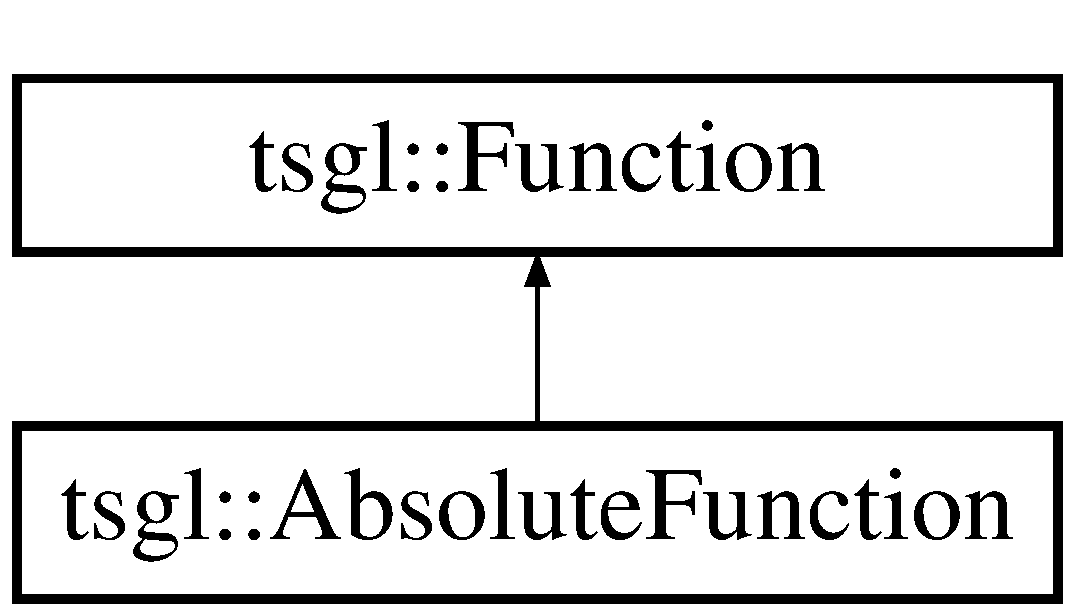
\includegraphics[height=2.000000cm]{classtsgl_1_1_absolute_function}
\end{center}
\end{figure}
\subsection*{Public Member Functions}
\begin{DoxyCompactItemize}
\item 
virtual Decimal \hyperlink{classtsgl_1_1_absolute_function_a29b4dd051d17e92b4f2d64b492a6ca19}{value\+At} (Decimal x) const 
\begin{DoxyCompactList}\small\item\em Method to determine the value of \hyperlink{classtsgl_1_1_absolute_function}{Absolute\+Function}. \end{DoxyCompactList}\end{DoxyCompactItemize}


\subsection{Detailed Description}
\hyperlink{classtsgl_1_1_function}{Function} to compute the absolute value of the input. 

\subsection{Member Function Documentation}
\hypertarget{classtsgl_1_1_absolute_function_a29b4dd051d17e92b4f2d64b492a6ca19}{}\index{tsgl\+::\+Absolute\+Function@{tsgl\+::\+Absolute\+Function}!value\+At@{value\+At}}
\index{value\+At@{value\+At}!tsgl\+::\+Absolute\+Function@{tsgl\+::\+Absolute\+Function}}
\subsubsection[{value\+At}]{\setlength{\rightskip}{0pt plus 5cm}virtual Decimal tsgl\+::\+Absolute\+Function\+::value\+At (
\begin{DoxyParamCaption}
\item[{Decimal}]{x}
\end{DoxyParamCaption}
) const\hspace{0.3cm}{\ttfamily [inline]}, {\ttfamily [virtual]}}\label{classtsgl_1_1_absolute_function_a29b4dd051d17e92b4f2d64b492a6ca19}


Method to determine the value of \hyperlink{classtsgl_1_1_absolute_function}{Absolute\+Function}. 

\begin{DoxyReturn}{Returns}
The absolute value of {\itshape x}. 
\end{DoxyReturn}


Implements \hyperlink{classtsgl_1_1_function_affb7b3b19a04efefa29a9870d666e912}{tsgl\+::\+Function}.



The documentation for this class was generated from the following file\+:\begin{DoxyCompactItemize}
\item 
Function.\+h\end{DoxyCompactItemize}

\hypertarget{class_ant_farm}{}\section{Ant\+Farm Class Reference}
\label{class_ant_farm}\index{Ant\+Farm@{Ant\+Farm}}


Display one or more of Langton\textquotesingle{}s Ant!  




{\ttfamily \#include $<$Ant\+Farm.\+h$>$}

\subsection*{Public Member Functions}
\begin{DoxyCompactItemize}
\item 
\hyperlink{class_ant_farm_af788cadd7ccb425440294af033fc6159}{Ant\+Farm} (int w, int h, int s, \hyperlink{classtsgl_1_1_canvas}{Canvas} $\ast$can)
\begin{DoxyCompactList}\small\item\em Explicitly constructs an \hyperlink{class_ant_farm}{Ant\+Farm} object. \end{DoxyCompactList}\item 
\hyperlink{class_ant_farm_a0b4fee39eeac74f6d866344a5cf221c4}{$\sim$\+Ant\+Farm} ()
\begin{DoxyCompactList}\small\item\em Destroy an \hyperlink{class_ant_farm}{Ant\+Farm} object. \end{DoxyCompactList}\item 
void \hyperlink{class_ant_farm_a30370a9e93b1534806ce47905359cf86}{add\+Ant} (int x, int y, int r, int g, int b, int d)
\begin{DoxyCompactList}\small\item\em Add an ant. \end{DoxyCompactList}\item 
void \hyperlink{class_ant_farm_a083c7d1e148cf6f36c2378795b239290}{move\+Ants} ()
\begin{DoxyCompactList}\small\item\em Move the ants. \end{DoxyCompactList}\item 
void \hyperlink{class_ant_farm_a5b333a275f2e0ff8700932fdfa04df08}{set\+Shading} (bool b)
\begin{DoxyCompactList}\small\item\em Shade the ants. \end{DoxyCompactList}\item 
void \hyperlink{class_ant_farm_ad4d22511ce20db2dedc7d61d4ca42e66}{set\+Parallel} (bool b)
\begin{DoxyCompactList}\small\item\em Moves the ants in parallel. \end{DoxyCompactList}\end{DoxyCompactItemize}
\subsection*{Public Attributes}
\begin{DoxyCompactItemize}
\item 
\mbox{\Hypertarget{class_ant_farm_a6b2f02189482c7bacde7ddaf9794de68}\label{class_ant_farm_a6b2f02189482c7bacde7ddaf9794de68}} 
\hyperlink{class_langton_ant}{Langton\+Ant} $\ast$$\ast$ {\bfseries ants}
\item 
\mbox{\Hypertarget{class_ant_farm_a073edbf5a8226b15d8a6c962612bab5a}\label{class_ant_farm_a073edbf5a8226b15d8a6c962612bab5a}} 
int {\bfseries width}
\item 
\mbox{\Hypertarget{class_ant_farm_a63cce968f831f6ea3cc699fae67295d4}\label{class_ant_farm_a63cce968f831f6ea3cc699fae67295d4}} 
int {\bfseries height}
\item 
\mbox{\Hypertarget{class_ant_farm_a67f9ece3e5d9b89269fea33e8252e77c}\label{class_ant_farm_a67f9ece3e5d9b89269fea33e8252e77c}} 
int {\bfseries size}
\item 
\mbox{\Hypertarget{class_ant_farm_a6609ec5efe8166f023ba360f415afe77}\label{class_ant_farm_a6609ec5efe8166f023ba360f415afe77}} 
int {\bfseries cap}
\item 
\mbox{\Hypertarget{class_ant_farm_aa617c67c5017be560f6da73d1ef15a1b}\label{class_ant_farm_aa617c67c5017be560f6da73d1ef15a1b}} 
\hyperlink{classtsgl_1_1_canvas}{Canvas} $\ast$ {\bfseries can}
\end{DoxyCompactItemize}


\subsection{Detailed Description}
Display one or more of Langton\textquotesingle{}s Ant! 

Contains the data and method needed in order to hold and move around one or more \hyperlink{class_langton_ant}{Langton\+Ant} objects.

You can have one \hyperlink{class_langton_ant}{Langton\+Ant}, or multiple.

You can move them in parallel, or in sequence.

You can also shade the colors of each \hyperlink{class_langton_ant}{Langton\+Ant}. 

\subsection{Constructor \& Destructor Documentation}
\mbox{\Hypertarget{class_ant_farm_af788cadd7ccb425440294af033fc6159}\label{class_ant_farm_af788cadd7ccb425440294af033fc6159}} 
\index{Ant\+Farm@{Ant\+Farm}!Ant\+Farm@{Ant\+Farm}}
\index{Ant\+Farm@{Ant\+Farm}!Ant\+Farm@{Ant\+Farm}}
\subsubsection{\texorpdfstring{Ant\+Farm()}{AntFarm()}}
{\footnotesize\ttfamily Ant\+Farm\+::\+Ant\+Farm (\begin{DoxyParamCaption}\item[{int}]{w,  }\item[{int}]{h,  }\item[{int}]{s,  }\item[{\hyperlink{classtsgl_1_1_canvas}{Canvas} $\ast$}]{can }\end{DoxyParamCaption})}



Explicitly constructs an \hyperlink{class_ant_farm}{Ant\+Farm} object. 

Explicit constructor for the \hyperlink{class_ant_farm}{Ant\+Farm} class. 
\begin{DoxyParams}{Parameters}
{\em w} & The width of the \hyperlink{class_ant_farm}{Ant\+Farm} object. \\
\hline
{\em h} & The height of the \hyperlink{class_ant_farm}{Ant\+Farm} object. \\
\hline
{\em s} & The size of the \hyperlink{class_ant_farm}{Ant\+Farm} object (how many ants are going to be in the \hyperlink{class_ant_farm}{Ant\+Farm} object). \\
\hline
{\em can} & Pointer to the Canvas to draw to. \\
\hline
\end{DoxyParams}
\mbox{\Hypertarget{class_ant_farm_a0b4fee39eeac74f6d866344a5cf221c4}\label{class_ant_farm_a0b4fee39eeac74f6d866344a5cf221c4}} 
\index{Ant\+Farm@{Ant\+Farm}!````~Ant\+Farm@{$\sim$\+Ant\+Farm}}
\index{````~Ant\+Farm@{$\sim$\+Ant\+Farm}!Ant\+Farm@{Ant\+Farm}}
\subsubsection{\texorpdfstring{$\sim$\+Ant\+Farm()}{~AntFarm()}}
{\footnotesize\ttfamily Ant\+Farm\+::$\sim$\+Ant\+Farm (\begin{DoxyParamCaption}{ }\end{DoxyParamCaption})}



Destroy an \hyperlink{class_ant_farm}{Ant\+Farm} object. 

Destructor for the \hyperlink{class_ant_farm}{Ant\+Farm} class. \begin{DoxyReturn}{Returns}
Frees up any allocated memory to an \hyperlink{class_ant_farm}{Ant\+Farm} object. 
\end{DoxyReturn}


\subsection{Member Function Documentation}
\mbox{\Hypertarget{class_ant_farm_a30370a9e93b1534806ce47905359cf86}\label{class_ant_farm_a30370a9e93b1534806ce47905359cf86}} 
\index{Ant\+Farm@{Ant\+Farm}!add\+Ant@{add\+Ant}}
\index{add\+Ant@{add\+Ant}!Ant\+Farm@{Ant\+Farm}}
\subsubsection{\texorpdfstring{add\+Ant()}{addAnt()}}
{\footnotesize\ttfamily void Ant\+Farm\+::add\+Ant (\begin{DoxyParamCaption}\item[{int}]{x,  }\item[{int}]{y,  }\item[{int}]{r,  }\item[{int}]{g,  }\item[{int}]{b,  }\item[{int}]{d }\end{DoxyParamCaption})}



Add an ant. 

Adds a \hyperlink{class_langton_ant}{Langton\+Ant} to the \hyperlink{class_ant_farm}{Ant\+Farm} with the specified arguments. 
\begin{DoxyParams}{Parameters}
{\em x} & The x coordinate of the \hyperlink{class_langton_ant}{Langton\+Ant}. \\
\hline
{\em y} & The y coordinate of the \hyperlink{class_langton_ant}{Langton\+Ant}. \\
\hline
{\em r} & Red component of the color of the \hyperlink{class_langton_ant}{Langton\+Ant}. \\
\hline
{\em g} & Green component of the color of the \hyperlink{class_langton_ant}{Langton\+Ant}. \\
\hline
{\em b} & Blue component of the color of the \hyperlink{class_langton_ant}{Langton\+Ant}. \\
\hline
{\em d} & The direction of the \hyperlink{class_langton_ant}{Langton\+Ant}. \\
\hline
\end{DoxyParams}
\mbox{\Hypertarget{class_ant_farm_a083c7d1e148cf6f36c2378795b239290}\label{class_ant_farm_a083c7d1e148cf6f36c2378795b239290}} 
\index{Ant\+Farm@{Ant\+Farm}!move\+Ants@{move\+Ants}}
\index{move\+Ants@{move\+Ants}!Ant\+Farm@{Ant\+Farm}}
\subsubsection{\texorpdfstring{move\+Ants()}{moveAnts()}}
{\footnotesize\ttfamily void Ant\+Farm\+::move\+Ants (\begin{DoxyParamCaption}{ }\end{DoxyParamCaption})}



Move the ants. 

Move the Langton\+Ants that are currently in the \hyperlink{class_ant_farm}{Ant\+Farm} object. \mbox{\Hypertarget{class_ant_farm_ad4d22511ce20db2dedc7d61d4ca42e66}\label{class_ant_farm_ad4d22511ce20db2dedc7d61d4ca42e66}} 
\index{Ant\+Farm@{Ant\+Farm}!set\+Parallel@{set\+Parallel}}
\index{set\+Parallel@{set\+Parallel}!Ant\+Farm@{Ant\+Farm}}
\subsubsection{\texorpdfstring{set\+Parallel()}{setParallel()}}
{\footnotesize\ttfamily void Ant\+Farm\+::set\+Parallel (\begin{DoxyParamCaption}\item[{bool}]{b }\end{DoxyParamCaption})}



Moves the ants in parallel. 

Determines if we should move the \hyperlink{class_langton_ant}{Langton\+Ant(s)} in parallel or not. 
\begin{DoxyParams}{Parameters}
{\em b} & A boolean determining if we should move the \hyperlink{class_langton_ant}{Langton\+Ant(s)} in parallel or not. \\
\hline
\end{DoxyParams}
\mbox{\Hypertarget{class_ant_farm_a5b333a275f2e0ff8700932fdfa04df08}\label{class_ant_farm_a5b333a275f2e0ff8700932fdfa04df08}} 
\index{Ant\+Farm@{Ant\+Farm}!set\+Shading@{set\+Shading}}
\index{set\+Shading@{set\+Shading}!Ant\+Farm@{Ant\+Farm}}
\subsubsection{\texorpdfstring{set\+Shading()}{setShading()}}
{\footnotesize\ttfamily void Ant\+Farm\+::set\+Shading (\begin{DoxyParamCaption}\item[{bool}]{b }\end{DoxyParamCaption})}



Shade the ants. 

Determines if we should shade the \hyperlink{class_langton_ant}{Langton\+Ant(s)} so that they have a darker color or not. 
\begin{DoxyParams}{Parameters}
{\em b} & A boolean determining if we should shade the \hyperlink{class_langton_ant}{Langton\+Ant(s)} or not. \\
\hline
\end{DoxyParams}


The documentation for this class was generated from the following files\+:\begin{DoxyCompactItemize}
\item 
/home/sth5/test/\+T\+S\+G\+L/src/examples/\+Langton/Ant\+Farm.\+h\item 
/home/sth5/test/\+T\+S\+G\+L/src/examples/\+Langton/Ant\+Farm.\+cpp\end{DoxyCompactItemize}

\hypertarget{classtsgl_1_1_array}{}\section{tsgl\+:\+:Array$<$ Item $>$ Class Template Reference}
\label{classtsgl_1_1_array}\index{tsgl\+::\+Array$<$ Item $>$@{tsgl\+::\+Array$<$ Item $>$}}


Custom internal array used by \hyperlink{classtsgl_1_1_canvas}{Canvas}.  




{\ttfamily \#include $<$Array.\+h$>$}

\subsection*{Public Member Functions}
\begin{DoxyCompactItemize}
\item 
\hyperlink{classtsgl_1_1_array_acc018fe6db37e7eb5df06789de034904}{Array} (unsigned int \hyperlink{classtsgl_1_1_array_a590e6a7c3bbf1470aff97a83f23f83c3}{size})
\begin{DoxyCompactList}\small\item\em \hyperlink{classtsgl_1_1_array}{Array} constructor method. \end{DoxyCompactList}\item 
virtual \hyperlink{classtsgl_1_1_array_aeef4dedf813a5bac862e19c55dee9069}{$\sim$\+Array} ()
\begin{DoxyCompactList}\small\item\em \hyperlink{classtsgl_1_1_array}{Array} destructor method. \end{DoxyCompactList}\item 
\hypertarget{classtsgl_1_1_array_acc5f5148a71c7f606be6cc337116bad6}{}void \hyperlink{classtsgl_1_1_array_acc5f5148a71c7f606be6cc337116bad6}{clear} ()\label{classtsgl_1_1_array_acc5f5148a71c7f606be6cc337116bad6}

\begin{DoxyCompactList}\small\item\em Empties the internal array and resets it, deleting contained objects. \end{DoxyCompactList}\item 
void \hyperlink{classtsgl_1_1_array_afe9d7b1dd294e8c74280b961ac84ac10}{shallow\+Clear} ()
\begin{DoxyCompactList}\small\item\em Empties the internal array but does not delete the objects it contains. \end{DoxyCompactList}\item 
const Item \& \hyperlink{classtsgl_1_1_array_a991ddcad3de14bd96009f4f90b648f6d}{operator\mbox{[}$\,$\mbox{]}} (unsigned int index) const 
\begin{DoxyCompactList}\small\item\em Returns the item at index {\ttfamily index}. \end{DoxyCompactList}\item 
Item \& \hyperlink{classtsgl_1_1_array_ae98fe9dc7998ec3b694150a8f70d8423}{operator\mbox{[}$\,$\mbox{]}} (unsigned int index)
\begin{DoxyCompactList}\small\item\em Returns the item at index {\ttfamily index}. \end{DoxyCompactList}\item 
\hypertarget{classtsgl_1_1_array_a590e6a7c3bbf1470aff97a83f23f83c3}{}unsigned int \hyperlink{classtsgl_1_1_array_a590e6a7c3bbf1470aff97a83f23f83c3}{size} () const \label{classtsgl_1_1_array_a590e6a7c3bbf1470aff97a83f23f83c3}

\begin{DoxyCompactList}\small\item\em Returns the number of items in the internal array. \end{DoxyCompactList}\item 
\hypertarget{classtsgl_1_1_array_a483497b4a309ccbf7e817c7ac1eff95a}{}unsigned int \hyperlink{classtsgl_1_1_array_a483497b4a309ccbf7e817c7ac1eff95a}{capacity} () const \label{classtsgl_1_1_array_a483497b4a309ccbf7e817c7ac1eff95a}

\begin{DoxyCompactList}\small\item\em Returns the maximum amount of items the internal array can store. \end{DoxyCompactList}\item 
\hypertarget{classtsgl_1_1_array_a2676cc880c5638849db5777f33680c9c}{}bool \hyperlink{classtsgl_1_1_array_a2676cc880c5638849db5777f33680c9c}{is\+Empty} () const \label{classtsgl_1_1_array_a2676cc880c5638849db5777f33680c9c}

\begin{DoxyCompactList}\small\item\em Returns true if the internal array contains no items, false otherwise. \end{DoxyCompactList}\item 
Item \hyperlink{classtsgl_1_1_array_aca25dfa4218b2c872d1e1cd2a1a32caa}{push} (Item item)
\begin{DoxyCompactList}\small\item\em Adds the item {\ttfamily item} to the end of the internal array. \end{DoxyCompactList}\end{DoxyCompactItemize}


\subsection{Detailed Description}
\subsubsection*{template$<$typename Item$>$class tsgl\+::\+Array$<$ Item $>$}

Custom internal array used by \hyperlink{classtsgl_1_1_canvas}{Canvas}. 

The \hyperlink{classtsgl_1_1_array}{Array} class manages a custom array for storing shapes to be drawn. It contains utility methods for checking if the internal array is empty, methods for emptying and resetting the internal array, and a subscript operator for accessing individual elements. \begin{DoxyNote}{Note}
The \hyperlink{classtsgl_1_1_array}{Array} has wrap-\/around behavior, behaving similarly to a circular queue. 

If a new shape is pushed into a full \hyperlink{classtsgl_1_1_array}{Array}, the first element is deleted and the pointer to the first element is incremented. 
\end{DoxyNote}


\subsection{Constructor \& Destructor Documentation}
\hypertarget{classtsgl_1_1_array_acc018fe6db37e7eb5df06789de034904}{}\index{tsgl\+::\+Array@{tsgl\+::\+Array}!Array@{Array}}
\index{Array@{Array}!tsgl\+::\+Array@{tsgl\+::\+Array}}
\subsubsection[{Array}]{\setlength{\rightskip}{0pt plus 5cm}template$<$typename Item$>$ {\bf tsgl\+::\+Array}$<$ Item $>$\+::{\bf Array} (
\begin{DoxyParamCaption}
\item[{unsigned int}]{size}
\end{DoxyParamCaption}
)\hspace{0.3cm}{\ttfamily [inline]}}\label{classtsgl_1_1_array_acc018fe6db37e7eb5df06789de034904}


\hyperlink{classtsgl_1_1_array}{Array} constructor method. 


\begin{DoxyParams}{Parameters}
{\em size} & The maximum capacity of the \hyperlink{classtsgl_1_1_array}{Array}. \\
\hline
\end{DoxyParams}
\begin{DoxyReturn}{Returns}
An \hyperlink{classtsgl_1_1_array}{Array} with capacity {\ttfamily size}. 
\end{DoxyReturn}
\hypertarget{classtsgl_1_1_array_aeef4dedf813a5bac862e19c55dee9069}{}\index{tsgl\+::\+Array@{tsgl\+::\+Array}!````~Array@{$\sim$\+Array}}
\index{````~Array@{$\sim$\+Array}!tsgl\+::\+Array@{tsgl\+::\+Array}}
\subsubsection[{$\sim$\+Array}]{\setlength{\rightskip}{0pt plus 5cm}template$<$typename Item$>$ virtual {\bf tsgl\+::\+Array}$<$ Item $>$\+::$\sim${\bf Array} (
\begin{DoxyParamCaption}
{}
\end{DoxyParamCaption}
)\hspace{0.3cm}{\ttfamily [inline]}, {\ttfamily [virtual]}}\label{classtsgl_1_1_array_aeef4dedf813a5bac862e19c55dee9069}


\hyperlink{classtsgl_1_1_array}{Array} destructor method. 

Frees up memory allocated to an \hyperlink{classtsgl_1_1_array}{Array} instance. 

\subsection{Member Function Documentation}
\hypertarget{classtsgl_1_1_array_a991ddcad3de14bd96009f4f90b648f6d}{}\index{tsgl\+::\+Array@{tsgl\+::\+Array}!operator\mbox{[}$\,$\mbox{]}@{operator[]}}
\index{operator\mbox{[}$\,$\mbox{]}@{operator[]}!tsgl\+::\+Array@{tsgl\+::\+Array}}
\subsubsection[{operator[]}]{\setlength{\rightskip}{0pt plus 5cm}template$<$typename Item$>$ const Item\& {\bf tsgl\+::\+Array}$<$ Item $>$\+::operator\mbox{[}$\,$\mbox{]} (
\begin{DoxyParamCaption}
\item[{unsigned int}]{index}
\end{DoxyParamCaption}
) const\hspace{0.3cm}{\ttfamily [inline]}}\label{classtsgl_1_1_array_a991ddcad3de14bd96009f4f90b648f6d}


Returns the item at index {\ttfamily index}. 


\begin{DoxyParams}{Parameters}
{\em index} & The index of the item in the internal array. \\
\hline
\end{DoxyParams}
\begin{DoxyNote}{Note}
This is the read version of the subscript operator. 
\end{DoxyNote}
\begin{DoxyReturn}{Returns}
The item at index {\ttfamily index}. 
\end{DoxyReturn}
\hypertarget{classtsgl_1_1_array_ae98fe9dc7998ec3b694150a8f70d8423}{}\index{tsgl\+::\+Array@{tsgl\+::\+Array}!operator\mbox{[}$\,$\mbox{]}@{operator[]}}
\index{operator\mbox{[}$\,$\mbox{]}@{operator[]}!tsgl\+::\+Array@{tsgl\+::\+Array}}
\subsubsection[{operator[]}]{\setlength{\rightskip}{0pt plus 5cm}template$<$typename Item$>$ Item\& {\bf tsgl\+::\+Array}$<$ Item $>$\+::operator\mbox{[}$\,$\mbox{]} (
\begin{DoxyParamCaption}
\item[{unsigned int}]{index}
\end{DoxyParamCaption}
)\hspace{0.3cm}{\ttfamily [inline]}}\label{classtsgl_1_1_array_ae98fe9dc7998ec3b694150a8f70d8423}


Returns the item at index {\ttfamily index}. 


\begin{DoxyParams}{Parameters}
{\em index} & The index of the item in the internal array. \\
\hline
\end{DoxyParams}
\begin{DoxyNote}{Note}
This is the write version of the subscript operator. 
\end{DoxyNote}
\begin{DoxyReturn}{Returns}
The item at index {\ttfamily index}. 
\end{DoxyReturn}
\hypertarget{classtsgl_1_1_array_aca25dfa4218b2c872d1e1cd2a1a32caa}{}\index{tsgl\+::\+Array@{tsgl\+::\+Array}!push@{push}}
\index{push@{push}!tsgl\+::\+Array@{tsgl\+::\+Array}}
\subsubsection[{push}]{\setlength{\rightskip}{0pt plus 5cm}template$<$typename Item$>$ Item {\bf tsgl\+::\+Array}$<$ Item $>$\+::push (
\begin{DoxyParamCaption}
\item[{Item}]{item}
\end{DoxyParamCaption}
)\hspace{0.3cm}{\ttfamily [inline]}}\label{classtsgl_1_1_array_aca25dfa4218b2c872d1e1cd2a1a32caa}


Adds the item {\ttfamily item} to the end of the internal array. 

\begin{DoxyNote}{Note}
If the internal array is full, \hyperlink{classtsgl_1_1_array_aca25dfa4218b2c872d1e1cd2a1a32caa}{push()} will remove the oldest item. 
\end{DoxyNote}

\begin{DoxyParams}{Parameters}
{\em item} & The item to add. \\
\hline
\end{DoxyParams}
\begin{DoxyReturn}{Returns}
The same item. 
\end{DoxyReturn}
\hypertarget{classtsgl_1_1_array_afe9d7b1dd294e8c74280b961ac84ac10}{}\index{tsgl\+::\+Array@{tsgl\+::\+Array}!shallow\+Clear@{shallow\+Clear}}
\index{shallow\+Clear@{shallow\+Clear}!tsgl\+::\+Array@{tsgl\+::\+Array}}
\subsubsection[{shallow\+Clear}]{\setlength{\rightskip}{0pt plus 5cm}template$<$typename Item$>$ void {\bf tsgl\+::\+Array}$<$ Item $>$\+::shallow\+Clear (
\begin{DoxyParamCaption}
{}
\end{DoxyParamCaption}
)\hspace{0.3cm}{\ttfamily [inline]}}\label{classtsgl_1_1_array_afe9d7b1dd294e8c74280b961ac84ac10}


Empties the internal array but does not delete the objects it contains. 

\begin{DoxyNote}{Note}
This method doesn\textquotesingle{}t delete the shapes inside of it; it only moves pointers around. 
\end{DoxyNote}
\begin{DoxyWarning}{Warning}
{\bfseries This will result in a memory leak if the objects are not pointed to anywhere else!} 
\end{DoxyWarning}


The documentation for this class was generated from the following file\+:\begin{DoxyCompactItemize}
\item 
Array.\+h\end{DoxyCompactItemize}

\hypertarget{classtsgl_1_1_arrow}{}\section{tsgl\+:\+:Arrow Class Reference}
\label{classtsgl_1_1_arrow}\index{tsgl\+::\+Arrow@{tsgl\+::\+Arrow}}


Draw a simple \hyperlink{classtsgl_1_1_arrow}{Arrow}.  




{\ttfamily \#include $<$Arrow.\+h$>$}

Inheritance diagram for tsgl\+:\+:Arrow\+:\begin{figure}[H]
\begin{center}
\leavevmode
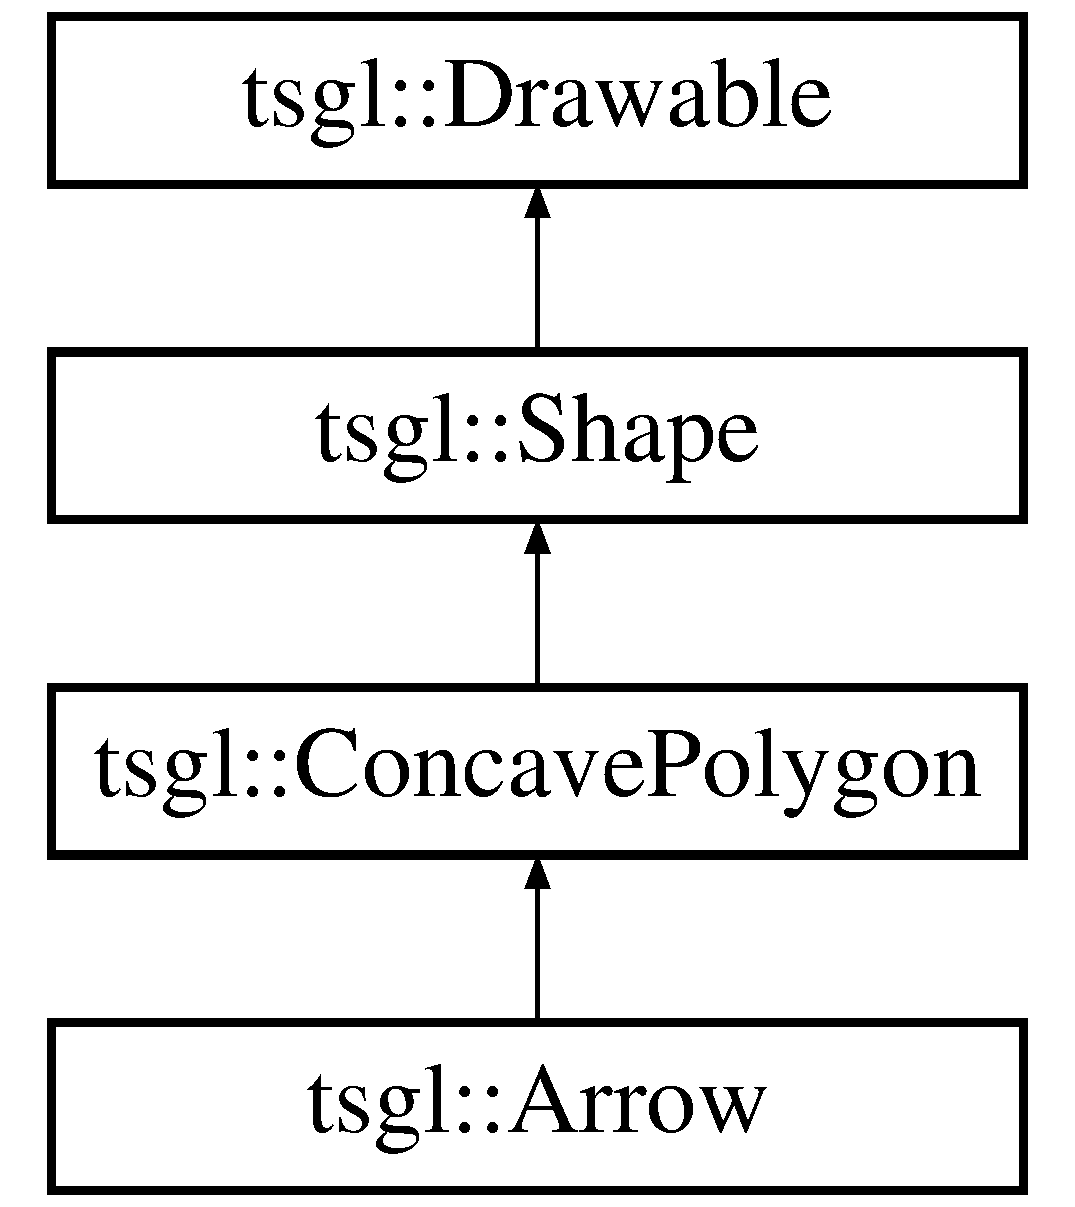
\includegraphics[height=4.000000cm]{classtsgl_1_1_arrow}
\end{center}
\end{figure}
\subsection*{Public Member Functions}
\begin{DoxyCompactItemize}
\item 
\hyperlink{classtsgl_1_1_arrow_a86e18cde9d0863fcb64ae7cdf0f6ddd1}{Arrow} (G\+Lfloat x1, G\+Lfloat y1, G\+Lfloat z1, G\+Lfloat x2, G\+Lfloat y2, G\+Lfloat z2, G\+Lfloat width, float yaw, float pitch, float roll, \hyperlink{structtsgl_1_1_color_float}{Color\+Float} color, bool double\+Arrow=false)
\begin{DoxyCompactList}\small\item\em Explicitly constructs a new \hyperlink{classtsgl_1_1_arrow}{Arrow}. \end{DoxyCompactList}\item 
\hyperlink{classtsgl_1_1_arrow_a44bf3a837e2f9c7b95673a1f9d9c2743}{Arrow} (G\+Lfloat x1, G\+Lfloat y1, G\+Lfloat z1, G\+Lfloat x2, G\+Lfloat y2, G\+Lfloat z2, G\+Lfloat width, float yaw, float pitch, float roll, \hyperlink{structtsgl_1_1_color_float}{Color\+Float} color\mbox{[}$\,$\mbox{]}, bool double\+Arrow=false)
\begin{DoxyCompactList}\small\item\em Explicitly constructs a new \hyperlink{classtsgl_1_1_arrow}{Arrow}. \end{DoxyCompactList}\item 
\hyperlink{classtsgl_1_1_arrow_ad084fce4677958a3211cea0bd94aab69}{Arrow} (float x, float y, float z, G\+Lfloat length, G\+Lfloat width, float yaw, float pitch, float roll, \hyperlink{structtsgl_1_1_color_float}{Color\+Float} color, bool double\+Arrow=false)
\begin{DoxyCompactList}\small\item\em Explicitly constructs a new \hyperlink{classtsgl_1_1_arrow}{Arrow}. \end{DoxyCompactList}\item 
\hyperlink{classtsgl_1_1_arrow_adf3dc30a25b7094b25370455c1a86682}{Arrow} (float x, float y, float z, G\+Lfloat length, G\+Lfloat width, float yaw, float pitch, float roll, \hyperlink{structtsgl_1_1_color_float}{Color\+Float} color\mbox{[}$\,$\mbox{]}, bool double\+Arrow=false)
\begin{DoxyCompactList}\small\item\em Explicitly constructs a new \hyperlink{classtsgl_1_1_arrow}{Arrow}. \end{DoxyCompactList}\item 
void \hyperlink{classtsgl_1_1_arrow_aa87af78d9783fb12c07cbf5b93252b70}{set\+Length} (G\+Lfloat length)
\begin{DoxyCompactList}\small\item\em Replacement mutator for the length of the \hyperlink{classtsgl_1_1_arrow}{Arrow}. \end{DoxyCompactList}\item 
void \hyperlink{classtsgl_1_1_arrow_ab78359a1c86a74491116657d7c629872}{change\+Length\+By} (G\+Lfloat delta)
\begin{DoxyCompactList}\small\item\em Alteration mutator for the length of the \hyperlink{classtsgl_1_1_arrow}{Arrow}. \end{DoxyCompactList}\item 
G\+Lfloat \hyperlink{classtsgl_1_1_arrow_a26d2e0e5ab4856b1cd998ec5ebccb9bb}{get\+Length} ()
\begin{DoxyCompactList}\small\item\em Accessor for the length of the arrow from endpoint to endpoint. \end{DoxyCompactList}\item 
void \hyperlink{classtsgl_1_1_arrow_aea3e79fc0b28a86e6726b1a7c3caabfe}{set\+Width} (G\+Lfloat width)
\begin{DoxyCompactList}\small\item\em Replacement mutator for the width of the \hyperlink{classtsgl_1_1_arrow}{Arrow}. \end{DoxyCompactList}\item 
void \hyperlink{classtsgl_1_1_arrow_a5c36193adf4e20487bb596263bb622f2}{change\+Width\+By} (G\+Lfloat delta)
\begin{DoxyCompactList}\small\item\em Alteration mutator for the width of the \hyperlink{classtsgl_1_1_arrow}{Arrow}. \end{DoxyCompactList}\item 
G\+Lfloat \hyperlink{classtsgl_1_1_arrow_aac07322718ccdb64dfd847b300569142}{get\+Width} ()
\begin{DoxyCompactList}\small\item\em Accessor for the width of the arrow from widest point to widest point. \end{DoxyCompactList}\item 
void \hyperlink{classtsgl_1_1_arrow_a3e34a585aa8c598746d838f2516fe598}{set\+First\+Endpoint} (G\+Lfloat x, G\+Lfloat y, G\+Lfloat z)
\begin{DoxyCompactList}\small\item\em Mutator for the first endpoint coordinates of the \hyperlink{classtsgl_1_1_arrow}{Arrow}. \end{DoxyCompactList}\item 
void \hyperlink{classtsgl_1_1_arrow_a40040ab8b8cd21631f05ce1158bd2737}{set\+Second\+Endpoint} (G\+Lfloat x, G\+Lfloat y, G\+Lfloat z)
\begin{DoxyCompactList}\small\item\em Mutator for the second endpoint coordinates of the \hyperlink{classtsgl_1_1_arrow}{Arrow}. \end{DoxyCompactList}\item 
G\+Lfloat \hyperlink{classtsgl_1_1_arrow_a56f3590dcd62f465958f8b8e103dac4f}{get\+First\+EndpointX} ()
\begin{DoxyCompactList}\small\item\em Accessor for the x-\/coordinate of the \hyperlink{classtsgl_1_1_arrow}{Arrow}\textquotesingle{}s first endpoint. \end{DoxyCompactList}\item 
G\+Lfloat \hyperlink{classtsgl_1_1_arrow_ad83e321d535001bb4172b3009ff82f19}{get\+First\+EndpointY} ()
\begin{DoxyCompactList}\small\item\em Accessor for the y-\/coordinate of the \hyperlink{classtsgl_1_1_arrow}{Arrow}\textquotesingle{}s first endpoint. \end{DoxyCompactList}\item 
G\+Lfloat \hyperlink{classtsgl_1_1_arrow_aed21293d711501354026d26615146d03}{get\+First\+EndpointZ} ()
\begin{DoxyCompactList}\small\item\em Accessor for the z-\/coordinate of the \hyperlink{classtsgl_1_1_arrow}{Arrow}\textquotesingle{}s first endpoint. \end{DoxyCompactList}\item 
G\+Lfloat \hyperlink{classtsgl_1_1_arrow_aa17e6bfe5f41e5a13a8378b1819f108d}{get\+Second\+EndpointX} ()
\begin{DoxyCompactList}\small\item\em Accessor for the x-\/coordinate of the \hyperlink{classtsgl_1_1_arrow}{Arrow}\textquotesingle{}s second endpoint. \end{DoxyCompactList}\item 
G\+Lfloat \hyperlink{classtsgl_1_1_arrow_a512407b73d07ca147c6a94ff933922f7}{get\+Second\+EndpointY} ()
\begin{DoxyCompactList}\small\item\em Accessor for the y-\/coordinate of the \hyperlink{classtsgl_1_1_arrow}{Arrow}\textquotesingle{}s second endpoint. \end{DoxyCompactList}\item 
G\+Lfloat \hyperlink{classtsgl_1_1_arrow_adb3bf6b1bc75ab68bb89f5430358386a}{get\+Second\+EndpointZ} ()
\begin{DoxyCompactList}\small\item\em Accessor for the z-\/coordinate of the \hyperlink{classtsgl_1_1_arrow}{Arrow}\textquotesingle{}s second endpoint. \end{DoxyCompactList}\item 
virtual void \hyperlink{classtsgl_1_1_arrow_a4eabf87c29f3da697fe39006c45510b7}{set\+Color} (\hyperlink{structtsgl_1_1_color_float}{Color\+Float} c)
\begin{DoxyCompactList}\small\item\em Sets the \hyperlink{classtsgl_1_1_shape}{Shape} to a new color. \end{DoxyCompactList}\item 
virtual void \hyperlink{classtsgl_1_1_arrow_a7804a81f8ae4ae0208e80849438364f0}{set\+Color} (\hyperlink{structtsgl_1_1_color_float}{Color\+Float} c\mbox{[}$\,$\mbox{]})
\begin{DoxyCompactList}\small\item\em Sets the \hyperlink{classtsgl_1_1_arrow}{Arrow} to a new color. \end{DoxyCompactList}\item 
virtual void \hyperlink{classtsgl_1_1_arrow_a45f13b066c85baae9712730787f49fac}{get\+Colors} (std\+::vector$<$ \hyperlink{structtsgl_1_1_color_float}{Color\+Float} $>$ \&color\+Vec)
\begin{DoxyCompactList}\small\item\em Accessor for \hyperlink{classtsgl_1_1_arrow}{Arrow}\textquotesingle{}s colors. \end{DoxyCompactList}\end{DoxyCompactItemize}
\subsection*{Additional Inherited Members}


\subsection{Detailed Description}
Draw a simple \hyperlink{classtsgl_1_1_arrow}{Arrow}. 

\hyperlink{classtsgl_1_1_arrow}{Arrow} is a class for holding vertex data for a concave polygon shaped like an \hyperlink{classtsgl_1_1_arrow}{Arrow}. 

\subsection{Constructor \& Destructor Documentation}
\mbox{\Hypertarget{classtsgl_1_1_arrow_a86e18cde9d0863fcb64ae7cdf0f6ddd1}\label{classtsgl_1_1_arrow_a86e18cde9d0863fcb64ae7cdf0f6ddd1}} 
\index{tsgl\+::\+Arrow@{tsgl\+::\+Arrow}!Arrow@{Arrow}}
\index{Arrow@{Arrow}!tsgl\+::\+Arrow@{tsgl\+::\+Arrow}}
\subsubsection{\texorpdfstring{Arrow()}{Arrow()}\hspace{0.1cm}{\footnotesize\ttfamily [1/4]}}
{\footnotesize\ttfamily tsgl\+::\+Arrow\+::\+Arrow (\begin{DoxyParamCaption}\item[{G\+Lfloat}]{x1,  }\item[{G\+Lfloat}]{y1,  }\item[{G\+Lfloat}]{z1,  }\item[{G\+Lfloat}]{x2,  }\item[{G\+Lfloat}]{y2,  }\item[{G\+Lfloat}]{z2,  }\item[{G\+Lfloat}]{width,  }\item[{float}]{yaw,  }\item[{float}]{pitch,  }\item[{float}]{roll,  }\item[{\hyperlink{structtsgl_1_1_color_float}{Color\+Float}}]{color,  }\item[{bool}]{double\+Arrow = {\ttfamily false} }\end{DoxyParamCaption})}



Explicitly constructs a new \hyperlink{classtsgl_1_1_arrow}{Arrow}. 

This is the constructor for the \hyperlink{classtsgl_1_1_arrow}{Arrow} class. 
\begin{DoxyParams}{Parameters}
{\em x1} & The x coordinate of the first endpoint of the arrow. \\
\hline
{\em y1} & The y coordinate of the first endpoint of the arrow. \\
\hline
{\em z1} & The z coordinate of the first endpoint of the arrow. \\
\hline
{\em x2} & The x coordinate of the second endpoint of the arrow. \\
\hline
{\em y2} & The y coordinate of the second endpoint of the arrow. \\
\hline
{\em z2} & The z coordinate of the second endpoint of the arrow. \\
\hline
{\em width} & The width of the arrow at its widest points. \\
\hline
{\em yaw} & The yaw of the arrow. \\
\hline
{\em pitch} & The pitch of the arrow. \\
\hline
{\em roll} & The roll of the arrow. \\
\hline
{\em color} & A \hyperlink{structtsgl_1_1_color_float}{Color\+Float} for the color of the \hyperlink{classtsgl_1_1_arrow}{Arrow}. \\
\hline
\end{DoxyParams}
\begin{DoxyReturn}{Returns}
A new \hyperlink{classtsgl_1_1_arrow}{Arrow} with the specified endpoints and color. 
\end{DoxyReturn}
\mbox{\Hypertarget{classtsgl_1_1_arrow_a44bf3a837e2f9c7b95673a1f9d9c2743}\label{classtsgl_1_1_arrow_a44bf3a837e2f9c7b95673a1f9d9c2743}} 
\index{tsgl\+::\+Arrow@{tsgl\+::\+Arrow}!Arrow@{Arrow}}
\index{Arrow@{Arrow}!tsgl\+::\+Arrow@{tsgl\+::\+Arrow}}
\subsubsection{\texorpdfstring{Arrow()}{Arrow()}\hspace{0.1cm}{\footnotesize\ttfamily [2/4]}}
{\footnotesize\ttfamily tsgl\+::\+Arrow\+::\+Arrow (\begin{DoxyParamCaption}\item[{G\+Lfloat}]{x1,  }\item[{G\+Lfloat}]{y1,  }\item[{G\+Lfloat}]{z1,  }\item[{G\+Lfloat}]{x2,  }\item[{G\+Lfloat}]{y2,  }\item[{G\+Lfloat}]{z2,  }\item[{G\+Lfloat}]{width,  }\item[{float}]{yaw,  }\item[{float}]{pitch,  }\item[{float}]{roll,  }\item[{\hyperlink{structtsgl_1_1_color_float}{Color\+Float}}]{color\mbox{[}$\,$\mbox{]},  }\item[{bool}]{double\+Arrow = {\ttfamily false} }\end{DoxyParamCaption})}



Explicitly constructs a new \hyperlink{classtsgl_1_1_arrow}{Arrow}. 

This is the constructor for the \hyperlink{classtsgl_1_1_arrow}{Arrow} class. 
\begin{DoxyParams}{Parameters}
{\em x1} & The x coordinate of the first endpoint of the arrow. \\
\hline
{\em y1} & The y coordinate of the first endpoint of the arrow. \\
\hline
{\em z1} & The z coordinate of the first endpoint of the arrow. \\
\hline
{\em x2} & The x coordinate of the second endpoint of the arrow. \\
\hline
{\em y2} & The y coordinate of the second endpoint of the arrow. \\
\hline
{\em z2} & The z coordinate of the second endpoint of the arrow. \\
\hline
{\em width} & The width of the arrow at its widest points. \\
\hline
{\em yaw} & The yaw of the arrow. \\
\hline
{\em pitch} & The pitch of the arrow. \\
\hline
{\em roll} & The roll of the arrow. \\
\hline
{\em color} & An array of Color\+Floats for the colors of the \hyperlink{classtsgl_1_1_arrow}{Arrow}. \\
\hline
\end{DoxyParams}
\begin{DoxyReturn}{Returns}
A new \hyperlink{classtsgl_1_1_arrow}{Arrow} with the specified endpoints and color. 
\end{DoxyReturn}
\mbox{\Hypertarget{classtsgl_1_1_arrow_ad084fce4677958a3211cea0bd94aab69}\label{classtsgl_1_1_arrow_ad084fce4677958a3211cea0bd94aab69}} 
\index{tsgl\+::\+Arrow@{tsgl\+::\+Arrow}!Arrow@{Arrow}}
\index{Arrow@{Arrow}!tsgl\+::\+Arrow@{tsgl\+::\+Arrow}}
\subsubsection{\texorpdfstring{Arrow()}{Arrow()}\hspace{0.1cm}{\footnotesize\ttfamily [3/4]}}
{\footnotesize\ttfamily tsgl\+::\+Arrow\+::\+Arrow (\begin{DoxyParamCaption}\item[{float}]{x,  }\item[{float}]{y,  }\item[{float}]{z,  }\item[{G\+Lfloat}]{length,  }\item[{G\+Lfloat}]{width,  }\item[{float}]{yaw,  }\item[{float}]{pitch,  }\item[{float}]{roll,  }\item[{\hyperlink{structtsgl_1_1_color_float}{Color\+Float}}]{color,  }\item[{bool}]{double\+Arrow = {\ttfamily false} }\end{DoxyParamCaption})}



Explicitly constructs a new \hyperlink{classtsgl_1_1_arrow}{Arrow}. 

This is the constructor for the \hyperlink{classtsgl_1_1_arrow}{Arrow} class. 
\begin{DoxyParams}{Parameters}
{\em x} & The x coordinate of the center of the arrow. \\
\hline
{\em y} & The y coordinate of the center of the arrow. \\
\hline
{\em z} & The z coordinate of the center of the arrow. \\
\hline
{\em length} & The length of the arrow (from endpoint to endpoint). \\
\hline
{\em width} & The width of the arrow (between its widest points). \\
\hline
{\em yaw} & The yaw of the arrow. \\
\hline
{\em pitch} & The pitch of the arrow. \\
\hline
{\em roll} & The roll of the arrow. \\
\hline
{\em color} & A \hyperlink{structtsgl_1_1_color_float}{Color\+Float} for the color of the \hyperlink{classtsgl_1_1_arrow}{Arrow}. \\
\hline
\end{DoxyParams}
\begin{DoxyReturn}{Returns}
A new \hyperlink{classtsgl_1_1_arrow}{Arrow} with the specified length and color. 
\end{DoxyReturn}
\begin{DoxyNote}{Note}
At 0,0,0 yaw,pitch,roll, the arrow will be drawn directly parallel to the x-\/axis as a plane perpindicular to the z-\/axis. 
\end{DoxyNote}
\mbox{\Hypertarget{classtsgl_1_1_arrow_adf3dc30a25b7094b25370455c1a86682}\label{classtsgl_1_1_arrow_adf3dc30a25b7094b25370455c1a86682}} 
\index{tsgl\+::\+Arrow@{tsgl\+::\+Arrow}!Arrow@{Arrow}}
\index{Arrow@{Arrow}!tsgl\+::\+Arrow@{tsgl\+::\+Arrow}}
\subsubsection{\texorpdfstring{Arrow()}{Arrow()}\hspace{0.1cm}{\footnotesize\ttfamily [4/4]}}
{\footnotesize\ttfamily tsgl\+::\+Arrow\+::\+Arrow (\begin{DoxyParamCaption}\item[{float}]{x,  }\item[{float}]{y,  }\item[{float}]{z,  }\item[{G\+Lfloat}]{length,  }\item[{G\+Lfloat}]{width,  }\item[{float}]{yaw,  }\item[{float}]{pitch,  }\item[{float}]{roll,  }\item[{\hyperlink{structtsgl_1_1_color_float}{Color\+Float}}]{color\mbox{[}$\,$\mbox{]},  }\item[{bool}]{double\+Arrow = {\ttfamily false} }\end{DoxyParamCaption})}



Explicitly constructs a new \hyperlink{classtsgl_1_1_arrow}{Arrow}. 

This is the constructor for the \hyperlink{classtsgl_1_1_arrow}{Arrow} class. 
\begin{DoxyParams}{Parameters}
{\em x} & The x coordinate of the center of the arrow. \\
\hline
{\em y} & The y coordinate of the center of the arrow. \\
\hline
{\em z} & The z coordinate of the center of the arrow. \\
\hline
{\em length} & The length of the arrow (from endpoint to endpoint). \\
\hline
{\em width} & The width of the arrow (between its widest points). \\
\hline
{\em yaw} & The yaw of the arrow. \\
\hline
{\em pitch} & The pitch of the arrow. \\
\hline
{\em roll} & The roll of the arrow. \\
\hline
{\em color} & An array of Color\+Floats for the colors of the \hyperlink{classtsgl_1_1_arrow}{Arrow}. \\
\hline
\end{DoxyParams}
\begin{DoxyReturn}{Returns}
A new \hyperlink{classtsgl_1_1_arrow}{Arrow} with the specified length and color. 
\end{DoxyReturn}
\begin{DoxyNote}{Note}
At 0,0,0 yaw,pitch,roll, the arrow will be drawn directly parallel to the x-\/axis as a plane perpindicular to the z-\/axis. 
\end{DoxyNote}


\subsection{Member Function Documentation}
\mbox{\Hypertarget{classtsgl_1_1_arrow_ab78359a1c86a74491116657d7c629872}\label{classtsgl_1_1_arrow_ab78359a1c86a74491116657d7c629872}} 
\index{tsgl\+::\+Arrow@{tsgl\+::\+Arrow}!change\+Length\+By@{change\+Length\+By}}
\index{change\+Length\+By@{change\+Length\+By}!tsgl\+::\+Arrow@{tsgl\+::\+Arrow}}
\subsubsection{\texorpdfstring{change\+Length\+By()}{changeLengthBy()}}
{\footnotesize\ttfamily void tsgl\+::\+Arrow\+::change\+Length\+By (\begin{DoxyParamCaption}\item[{G\+Lfloat}]{delta }\end{DoxyParamCaption})}



Alteration mutator for the length of the \hyperlink{classtsgl_1_1_arrow}{Arrow}. 

Alters the value of the my\+Length instance variable by delta and modifies the vertices array accordingly. 
\begin{DoxyParams}{Parameters}
{\em delta} & The difference between the old and new lengths of the \hyperlink{classtsgl_1_1_arrow}{Arrow}. \\
\hline
\end{DoxyParams}
\mbox{\Hypertarget{classtsgl_1_1_arrow_a5c36193adf4e20487bb596263bb622f2}\label{classtsgl_1_1_arrow_a5c36193adf4e20487bb596263bb622f2}} 
\index{tsgl\+::\+Arrow@{tsgl\+::\+Arrow}!change\+Width\+By@{change\+Width\+By}}
\index{change\+Width\+By@{change\+Width\+By}!tsgl\+::\+Arrow@{tsgl\+::\+Arrow}}
\subsubsection{\texorpdfstring{change\+Width\+By()}{changeWidthBy()}}
{\footnotesize\ttfamily void tsgl\+::\+Arrow\+::change\+Width\+By (\begin{DoxyParamCaption}\item[{G\+Lfloat}]{delta }\end{DoxyParamCaption})}



Alteration mutator for the width of the \hyperlink{classtsgl_1_1_arrow}{Arrow}. 

Alters the value of the my\+Width instance variable by delta and modifies the vertices array accordingly. 
\begin{DoxyParams}{Parameters}
{\em delta} & The difference between the old and new widths of the \hyperlink{classtsgl_1_1_arrow}{Arrow}. \\
\hline
\end{DoxyParams}


Referenced by get\+Length().

\mbox{\Hypertarget{classtsgl_1_1_arrow_a45f13b066c85baae9712730787f49fac}\label{classtsgl_1_1_arrow_a45f13b066c85baae9712730787f49fac}} 
\index{tsgl\+::\+Arrow@{tsgl\+::\+Arrow}!get\+Colors@{get\+Colors}}
\index{get\+Colors@{get\+Colors}!tsgl\+::\+Arrow@{tsgl\+::\+Arrow}}
\subsubsection{\texorpdfstring{get\+Colors()}{getColors()}}
{\footnotesize\ttfamily void tsgl\+::\+Arrow\+::get\+Colors (\begin{DoxyParamCaption}\item[{std\+::vector$<$ \hyperlink{structtsgl_1_1_color_float}{Color\+Float} $>$ \&}]{color\+Vec }\end{DoxyParamCaption})\hspace{0.3cm}{\ttfamily [virtual]}}



Accessor for \hyperlink{classtsgl_1_1_arrow}{Arrow}\textquotesingle{}s colors. 

Populates the reference parameter vector with a \hyperlink{structtsgl_1_1_color_float}{Color\+Float} for each end of \hyperlink{classtsgl_1_1_arrow}{Arrow}. 
\begin{DoxyParams}{Parameters}
{\em color\+Vec} & A vector of Color\+Floats to which the Color\+Floats associated with \hyperlink{classtsgl_1_1_arrow}{Arrow} will be pushed. \\
\hline
\end{DoxyParams}
\begin{DoxyNote}{Note}
Overrides \hyperlink{classtsgl_1_1_shape_a6f54fe4d049f69a287edf8335a9509f8}{Shape\+::get\+Colors()}. 
\end{DoxyNote}


Reimplemented from \hyperlink{classtsgl_1_1_shape_a6f54fe4d049f69a287edf8335a9509f8}{tsgl\+::\+Shape}.



Referenced by set\+Color().

\mbox{\Hypertarget{classtsgl_1_1_arrow_a56f3590dcd62f465958f8b8e103dac4f}\label{classtsgl_1_1_arrow_a56f3590dcd62f465958f8b8e103dac4f}} 
\index{tsgl\+::\+Arrow@{tsgl\+::\+Arrow}!get\+First\+EndpointX@{get\+First\+EndpointX}}
\index{get\+First\+EndpointX@{get\+First\+EndpointX}!tsgl\+::\+Arrow@{tsgl\+::\+Arrow}}
\subsubsection{\texorpdfstring{get\+First\+Endpoint\+X()}{getFirstEndpointX()}}
{\footnotesize\ttfamily float tsgl\+::\+Arrow\+::get\+First\+EndpointX (\begin{DoxyParamCaption}{ }\end{DoxyParamCaption})}



Accessor for the x-\/coordinate of the \hyperlink{classtsgl_1_1_arrow}{Arrow}\textquotesingle{}s first endpoint. 

Returns the value of the my\+Endpoint\+X1 instance variable, rotated around my\+Rotation\+Point by my\+Current\+Yaw\+Pitch\+Roll. \begin{DoxyReturn}{Returns}
my\+Endpoint\+X1, containing the value of the \hyperlink{classtsgl_1_1_arrow}{Arrow}\textquotesingle{}s first endpoint\textquotesingle{}s x-\/coordinate. 
\end{DoxyReturn}
\begin{DoxyNote}{Note}
See \hyperlink{classtsgl_1_1_drawable_a170ce95eaae8b19532420e42e9eb8abf}{Drawable\+::get\+Center\+X()} documentation for more info. 
\end{DoxyNote}


Referenced by get\+Width().

\mbox{\Hypertarget{classtsgl_1_1_arrow_ad83e321d535001bb4172b3009ff82f19}\label{classtsgl_1_1_arrow_ad83e321d535001bb4172b3009ff82f19}} 
\index{tsgl\+::\+Arrow@{tsgl\+::\+Arrow}!get\+First\+EndpointY@{get\+First\+EndpointY}}
\index{get\+First\+EndpointY@{get\+First\+EndpointY}!tsgl\+::\+Arrow@{tsgl\+::\+Arrow}}
\subsubsection{\texorpdfstring{get\+First\+Endpoint\+Y()}{getFirstEndpointY()}}
{\footnotesize\ttfamily float tsgl\+::\+Arrow\+::get\+First\+EndpointY (\begin{DoxyParamCaption}{ }\end{DoxyParamCaption})}



Accessor for the y-\/coordinate of the \hyperlink{classtsgl_1_1_arrow}{Arrow}\textquotesingle{}s first endpoint. 

Returns the value of the my\+Endpoint\+Y1 instance variable, rotated around my\+Rotation\+Point by my\+Current\+Yaw\+Pitch\+Roll. \begin{DoxyReturn}{Returns}
my\+Endpoint\+Y1, containing the value of the \hyperlink{classtsgl_1_1_arrow}{Arrow}\textquotesingle{}s first endpoint\textquotesingle{}s y-\/coordinate. 
\end{DoxyReturn}
\begin{DoxyNote}{Note}
See \hyperlink{classtsgl_1_1_drawable_ad78d781f078bab0f458892757f100e7f}{Drawable\+::get\+Center\+Y()} documentation for more info. 
\end{DoxyNote}


Referenced by get\+Width().

\mbox{\Hypertarget{classtsgl_1_1_arrow_aed21293d711501354026d26615146d03}\label{classtsgl_1_1_arrow_aed21293d711501354026d26615146d03}} 
\index{tsgl\+::\+Arrow@{tsgl\+::\+Arrow}!get\+First\+EndpointZ@{get\+First\+EndpointZ}}
\index{get\+First\+EndpointZ@{get\+First\+EndpointZ}!tsgl\+::\+Arrow@{tsgl\+::\+Arrow}}
\subsubsection{\texorpdfstring{get\+First\+Endpoint\+Z()}{getFirstEndpointZ()}}
{\footnotesize\ttfamily float tsgl\+::\+Arrow\+::get\+First\+EndpointZ (\begin{DoxyParamCaption}{ }\end{DoxyParamCaption})}



Accessor for the z-\/coordinate of the \hyperlink{classtsgl_1_1_arrow}{Arrow}\textquotesingle{}s first endpoint. 

Returns the value of the my\+Endpoint\+Z1 instance variable, rotated around my\+Rotation\+Point by my\+Current\+Yaw\+Pitch\+Roll. \begin{DoxyReturn}{Returns}
my\+Endpoint\+Z1, containing the value of the \hyperlink{classtsgl_1_1_arrow}{Arrow}\textquotesingle{}s first endpoint\textquotesingle{}s z-\/coordinate. 
\end{DoxyReturn}
\begin{DoxyNote}{Note}
See \hyperlink{classtsgl_1_1_drawable_a6a6c0441d94ffebd149f88ae3ab87ced}{Drawable\+::get\+Center\+Z()} documentation for more info. 
\end{DoxyNote}


Referenced by get\+Width().

\mbox{\Hypertarget{classtsgl_1_1_arrow_a26d2e0e5ab4856b1cd998ec5ebccb9bb}\label{classtsgl_1_1_arrow_a26d2e0e5ab4856b1cd998ec5ebccb9bb}} 
\index{tsgl\+::\+Arrow@{tsgl\+::\+Arrow}!get\+Length@{get\+Length}}
\index{get\+Length@{get\+Length}!tsgl\+::\+Arrow@{tsgl\+::\+Arrow}}
\subsubsection{\texorpdfstring{get\+Length()}{getLength()}}
{\footnotesize\ttfamily G\+Lfloat tsgl\+::\+Arrow\+::get\+Length (\begin{DoxyParamCaption}{ }\end{DoxyParamCaption})\hspace{0.3cm}{\ttfamily [inline]}}



Accessor for the length of the arrow from endpoint to endpoint. 

Returns the value of the my\+Length instance variable. \begin{DoxyReturn}{Returns}
my\+Length, containing the distance in 3D space between the two endpoints. 
\end{DoxyReturn}
\mbox{\Hypertarget{classtsgl_1_1_arrow_aa17e6bfe5f41e5a13a8378b1819f108d}\label{classtsgl_1_1_arrow_aa17e6bfe5f41e5a13a8378b1819f108d}} 
\index{tsgl\+::\+Arrow@{tsgl\+::\+Arrow}!get\+Second\+EndpointX@{get\+Second\+EndpointX}}
\index{get\+Second\+EndpointX@{get\+Second\+EndpointX}!tsgl\+::\+Arrow@{tsgl\+::\+Arrow}}
\subsubsection{\texorpdfstring{get\+Second\+Endpoint\+X()}{getSecondEndpointX()}}
{\footnotesize\ttfamily float tsgl\+::\+Arrow\+::get\+Second\+EndpointX (\begin{DoxyParamCaption}{ }\end{DoxyParamCaption})}



Accessor for the x-\/coordinate of the \hyperlink{classtsgl_1_1_arrow}{Arrow}\textquotesingle{}s second endpoint. 

Returns the value of the my\+Endpoint\+X2 instance variable, rotated around my\+Rotation\+Point by my\+Current\+Yaw\+Pitch\+Roll. \begin{DoxyReturn}{Returns}
my\+Endpoint\+X2, containing the value of the \hyperlink{classtsgl_1_1_arrow}{Arrow}\textquotesingle{}s second endpoint\textquotesingle{}s x-\/coordinate. 
\end{DoxyReturn}
\begin{DoxyNote}{Note}
See \hyperlink{classtsgl_1_1_drawable_a170ce95eaae8b19532420e42e9eb8abf}{Drawable\+::get\+Center\+X()} documentation for more info. 
\end{DoxyNote}


Referenced by get\+Width().

\mbox{\Hypertarget{classtsgl_1_1_arrow_a512407b73d07ca147c6a94ff933922f7}\label{classtsgl_1_1_arrow_a512407b73d07ca147c6a94ff933922f7}} 
\index{tsgl\+::\+Arrow@{tsgl\+::\+Arrow}!get\+Second\+EndpointY@{get\+Second\+EndpointY}}
\index{get\+Second\+EndpointY@{get\+Second\+EndpointY}!tsgl\+::\+Arrow@{tsgl\+::\+Arrow}}
\subsubsection{\texorpdfstring{get\+Second\+Endpoint\+Y()}{getSecondEndpointY()}}
{\footnotesize\ttfamily float tsgl\+::\+Arrow\+::get\+Second\+EndpointY (\begin{DoxyParamCaption}{ }\end{DoxyParamCaption})}



Accessor for the y-\/coordinate of the \hyperlink{classtsgl_1_1_arrow}{Arrow}\textquotesingle{}s second endpoint. 

Returns the value of the my\+Endpoint\+Y2 instance variable, rotated around my\+Rotation\+Point by my\+Current\+Yaw\+Pitch\+Roll. \begin{DoxyReturn}{Returns}
my\+Endpoint\+Y2, containing the value of the \hyperlink{classtsgl_1_1_arrow}{Arrow}\textquotesingle{}s second endpoint\textquotesingle{}s y-\/coordinate. 
\end{DoxyReturn}
\begin{DoxyNote}{Note}
See \hyperlink{classtsgl_1_1_drawable_ad78d781f078bab0f458892757f100e7f}{Drawable\+::get\+Center\+Y()} documentation for more info. 
\end{DoxyNote}


Referenced by get\+Width().

\mbox{\Hypertarget{classtsgl_1_1_arrow_adb3bf6b1bc75ab68bb89f5430358386a}\label{classtsgl_1_1_arrow_adb3bf6b1bc75ab68bb89f5430358386a}} 
\index{tsgl\+::\+Arrow@{tsgl\+::\+Arrow}!get\+Second\+EndpointZ@{get\+Second\+EndpointZ}}
\index{get\+Second\+EndpointZ@{get\+Second\+EndpointZ}!tsgl\+::\+Arrow@{tsgl\+::\+Arrow}}
\subsubsection{\texorpdfstring{get\+Second\+Endpoint\+Z()}{getSecondEndpointZ()}}
{\footnotesize\ttfamily float tsgl\+::\+Arrow\+::get\+Second\+EndpointZ (\begin{DoxyParamCaption}{ }\end{DoxyParamCaption})}



Accessor for the z-\/coordinate of the \hyperlink{classtsgl_1_1_arrow}{Arrow}\textquotesingle{}s second endpoint. 

Returns the value of the my\+Endpoint\+Z2 instance variable, rotated around my\+Rotation\+Point by my\+Current\+Yaw\+Pitch\+Roll. \begin{DoxyReturn}{Returns}
my\+Endpoint\+Z2, containing the value of the \hyperlink{classtsgl_1_1_arrow}{Arrow}\textquotesingle{}s second endpoint\textquotesingle{}s z-\/coordinate. 
\end{DoxyReturn}
\begin{DoxyNote}{Note}
See \hyperlink{classtsgl_1_1_drawable_a6a6c0441d94ffebd149f88ae3ab87ced}{Drawable\+::get\+Center\+Z()} documentation for more info. 
\end{DoxyNote}


Referenced by get\+Width().

\mbox{\Hypertarget{classtsgl_1_1_arrow_aac07322718ccdb64dfd847b300569142}\label{classtsgl_1_1_arrow_aac07322718ccdb64dfd847b300569142}} 
\index{tsgl\+::\+Arrow@{tsgl\+::\+Arrow}!get\+Width@{get\+Width}}
\index{get\+Width@{get\+Width}!tsgl\+::\+Arrow@{tsgl\+::\+Arrow}}
\subsubsection{\texorpdfstring{get\+Width()}{getWidth()}}
{\footnotesize\ttfamily G\+Lfloat tsgl\+::\+Arrow\+::get\+Width (\begin{DoxyParamCaption}{ }\end{DoxyParamCaption})\hspace{0.3cm}{\ttfamily [inline]}}



Accessor for the width of the arrow from widest point to widest point. 

Returns the value of the my\+Length instance variable. \begin{DoxyReturn}{Returns}
my\+Length, containing the distance in 3D space between the two endpoints. 
\end{DoxyReturn}
\mbox{\Hypertarget{classtsgl_1_1_arrow_a4eabf87c29f3da697fe39006c45510b7}\label{classtsgl_1_1_arrow_a4eabf87c29f3da697fe39006c45510b7}} 
\index{tsgl\+::\+Arrow@{tsgl\+::\+Arrow}!set\+Color@{set\+Color}}
\index{set\+Color@{set\+Color}!tsgl\+::\+Arrow@{tsgl\+::\+Arrow}}
\subsubsection{\texorpdfstring{set\+Color()}{setColor()}\hspace{0.1cm}{\footnotesize\ttfamily [1/2]}}
{\footnotesize\ttfamily virtual void tsgl\+::\+Arrow\+::set\+Color (\begin{DoxyParamCaption}\item[{\hyperlink{structtsgl_1_1_color_float}{Color\+Float}}]{c }\end{DoxyParamCaption})\hspace{0.3cm}{\ttfamily [inline]}, {\ttfamily [virtual]}}



Sets the \hyperlink{classtsgl_1_1_shape}{Shape} to a new color. 


\begin{DoxyParams}{Parameters}
{\em c} & The new \hyperlink{structtsgl_1_1_color_float}{Color\+Float}. \\
\hline
\end{DoxyParams}


Reimplemented from \hyperlink{classtsgl_1_1_shape_abdb01321cddfd2db1481eefbc2836f70}{tsgl\+::\+Shape}.

\mbox{\Hypertarget{classtsgl_1_1_arrow_a7804a81f8ae4ae0208e80849438364f0}\label{classtsgl_1_1_arrow_a7804a81f8ae4ae0208e80849438364f0}} 
\index{tsgl\+::\+Arrow@{tsgl\+::\+Arrow}!set\+Color@{set\+Color}}
\index{set\+Color@{set\+Color}!tsgl\+::\+Arrow@{tsgl\+::\+Arrow}}
\subsubsection{\texorpdfstring{set\+Color()}{setColor()}\hspace{0.1cm}{\footnotesize\ttfamily [2/2]}}
{\footnotesize\ttfamily void tsgl\+::\+Arrow\+::set\+Color (\begin{DoxyParamCaption}\item[{\hyperlink{structtsgl_1_1_color_float}{Color\+Float}}]{c\mbox{[}$\,$\mbox{]} }\end{DoxyParamCaption})\hspace{0.3cm}{\ttfamily [virtual]}}



Sets the \hyperlink{classtsgl_1_1_arrow}{Arrow} to a new color. 


\begin{DoxyParams}{Parameters}
{\em c} & The new array of Color\+Floats. \\
\hline
\end{DoxyParams}
\begin{DoxyNote}{Note}
Overrides \hyperlink{classtsgl_1_1_shape_ad7e554b5d4cea111ec518548b9f21388}{Shape\+::set\+Color(\+Color\+Float c\mbox{[}$\,$\mbox{]})}. 
\end{DoxyNote}


Reimplemented from \hyperlink{classtsgl_1_1_shape_ad7e554b5d4cea111ec518548b9f21388}{tsgl\+::\+Shape}.

\mbox{\Hypertarget{classtsgl_1_1_arrow_a3e34a585aa8c598746d838f2516fe598}\label{classtsgl_1_1_arrow_a3e34a585aa8c598746d838f2516fe598}} 
\index{tsgl\+::\+Arrow@{tsgl\+::\+Arrow}!set\+First\+Endpoint@{set\+First\+Endpoint}}
\index{set\+First\+Endpoint@{set\+First\+Endpoint}!tsgl\+::\+Arrow@{tsgl\+::\+Arrow}}
\subsubsection{\texorpdfstring{set\+First\+Endpoint()}{setFirstEndpoint()}}
{\footnotesize\ttfamily void tsgl\+::\+Arrow\+::set\+First\+Endpoint (\begin{DoxyParamCaption}\item[{G\+Lfloat}]{x,  }\item[{G\+Lfloat}]{y,  }\item[{G\+Lfloat}]{z }\end{DoxyParamCaption})}



Mutator for the first endpoint coordinates of the \hyperlink{classtsgl_1_1_arrow}{Arrow}. 

Sets the values of my\+Endpoint\+\_\+1 instance variables by the parameters and modifies the vertices array accordingly. 
\begin{DoxyParams}{Parameters}
{\em x} & The new x-\/coordinate of the first endpoint of the \hyperlink{classtsgl_1_1_arrow}{Arrow}. \\
\hline
{\em y} & The new y-\/coordinate of the first endpoint of the \hyperlink{classtsgl_1_1_arrow}{Arrow}. \\
\hline
{\em z} & The new z-\/coordinate of the first endpoint of the \hyperlink{classtsgl_1_1_arrow}{Arrow}. \\
\hline
\end{DoxyParams}


Referenced by get\+Width().

\mbox{\Hypertarget{classtsgl_1_1_arrow_aa87af78d9783fb12c07cbf5b93252b70}\label{classtsgl_1_1_arrow_aa87af78d9783fb12c07cbf5b93252b70}} 
\index{tsgl\+::\+Arrow@{tsgl\+::\+Arrow}!set\+Length@{set\+Length}}
\index{set\+Length@{set\+Length}!tsgl\+::\+Arrow@{tsgl\+::\+Arrow}}
\subsubsection{\texorpdfstring{set\+Length()}{setLength()}}
{\footnotesize\ttfamily void tsgl\+::\+Arrow\+::set\+Length (\begin{DoxyParamCaption}\item[{G\+Lfloat}]{length }\end{DoxyParamCaption})}



Replacement mutator for the length of the \hyperlink{classtsgl_1_1_arrow}{Arrow}. 

Sets the value of the my\+Length instance variable to the parameter, and modifies the vertices array accordingly. 
\begin{DoxyParams}{Parameters}
{\em length} & New length of the \hyperlink{classtsgl_1_1_arrow}{Arrow}, a float. \\
\hline
\end{DoxyParams}
\mbox{\Hypertarget{classtsgl_1_1_arrow_a40040ab8b8cd21631f05ce1158bd2737}\label{classtsgl_1_1_arrow_a40040ab8b8cd21631f05ce1158bd2737}} 
\index{tsgl\+::\+Arrow@{tsgl\+::\+Arrow}!set\+Second\+Endpoint@{set\+Second\+Endpoint}}
\index{set\+Second\+Endpoint@{set\+Second\+Endpoint}!tsgl\+::\+Arrow@{tsgl\+::\+Arrow}}
\subsubsection{\texorpdfstring{set\+Second\+Endpoint()}{setSecondEndpoint()}}
{\footnotesize\ttfamily void tsgl\+::\+Arrow\+::set\+Second\+Endpoint (\begin{DoxyParamCaption}\item[{G\+Lfloat}]{x,  }\item[{G\+Lfloat}]{y,  }\item[{G\+Lfloat}]{z }\end{DoxyParamCaption})}



Mutator for the second endpoint coordinates of the \hyperlink{classtsgl_1_1_arrow}{Arrow}. 

Sets the values of my\+Endpoint\+\_\+2 instance variables by the parameters and modifies the vertices array accordingly. 
\begin{DoxyParams}{Parameters}
{\em x} & The new x-\/coordinate of the second endpoint of the \hyperlink{classtsgl_1_1_arrow}{Arrow}. \\
\hline
{\em y} & The new y-\/coordinate of the second endpoint of the \hyperlink{classtsgl_1_1_arrow}{Arrow}. \\
\hline
{\em z} & The new z-\/coordinate of the second endpoint of the \hyperlink{classtsgl_1_1_arrow}{Arrow}. \\
\hline
\end{DoxyParams}


Referenced by get\+Width().

\mbox{\Hypertarget{classtsgl_1_1_arrow_aea3e79fc0b28a86e6726b1a7c3caabfe}\label{classtsgl_1_1_arrow_aea3e79fc0b28a86e6726b1a7c3caabfe}} 
\index{tsgl\+::\+Arrow@{tsgl\+::\+Arrow}!set\+Width@{set\+Width}}
\index{set\+Width@{set\+Width}!tsgl\+::\+Arrow@{tsgl\+::\+Arrow}}
\subsubsection{\texorpdfstring{set\+Width()}{setWidth()}}
{\footnotesize\ttfamily void tsgl\+::\+Arrow\+::set\+Width (\begin{DoxyParamCaption}\item[{G\+Lfloat}]{width }\end{DoxyParamCaption})}



Replacement mutator for the width of the \hyperlink{classtsgl_1_1_arrow}{Arrow}. 

Sets the value of the my\+Width instance variable to the parameter, and modifies the vertices array accordingly. 
\begin{DoxyParams}{Parameters}
{\em width} & New width of the \hyperlink{classtsgl_1_1_arrow}{Arrow}, a float. \\
\hline
\end{DoxyParams}


Referenced by get\+Length().



The documentation for this class was generated from the following files\+:\begin{DoxyCompactItemize}
\item 
Arrow.\+h\item 
Arrow.\+cpp\end{DoxyCompactItemize}

\hypertarget{classtsgl_1_1_background}{}\section{tsgl\+:\+:Background Class Reference}
\label{classtsgl_1_1_background}\index{tsgl\+::\+Background@{tsgl\+::\+Background}}


Draw a \hyperlink{classtsgl_1_1_background}{Background} for the \hyperlink{classtsgl_1_1_canvas}{Canvas} with colored pixels.  




{\ttfamily \#include $<$Background.\+h$>$}

Inheritance diagram for tsgl\+:\+:Background\+:\begin{figure}[H]
\begin{center}
\leavevmode
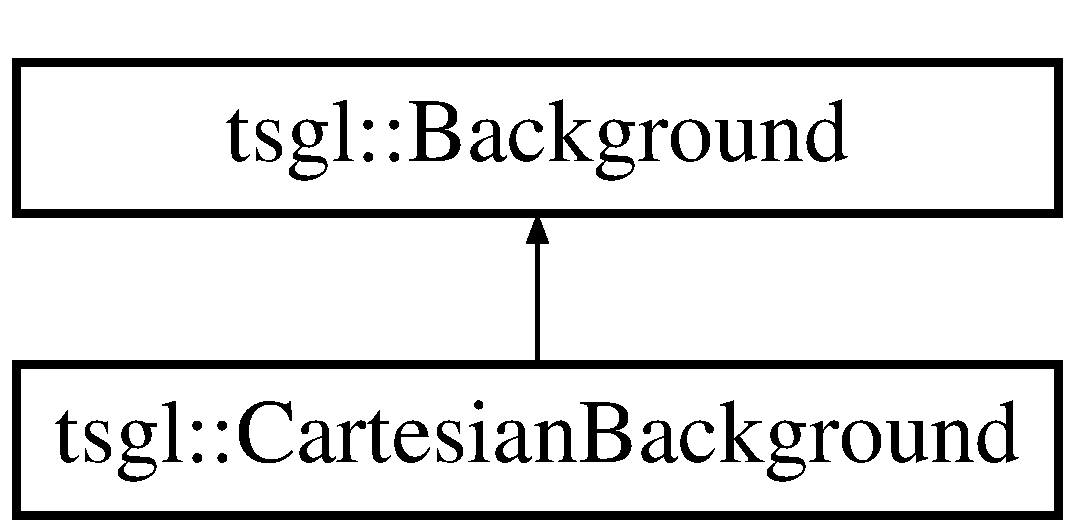
\includegraphics[height=2.000000cm]{classtsgl_1_1_background}
\end{center}
\end{figure}
\subsection*{Public Member Functions}
\begin{DoxyCompactItemize}
\item 
\hyperlink{classtsgl_1_1_background_a2cdb442cc62469acc31f6707ba96bea2}{Background} (G\+Lint width, G\+Lint height, const \hyperlink{structtsgl_1_1_color_float}{Color\+Float} \&c=W\+H\+I\+TE)
\begin{DoxyCompactList}\small\item\em Explicitly constructs a new \hyperlink{classtsgl_1_1_background}{Background}. \end{DoxyCompactList}\item 
virtual void \hyperlink{classtsgl_1_1_background_ae80545e3e31a4e5ec9d2796fc4f66ee8}{init} (Shader $\ast$shapeS, Shader $\ast$textS, Shader $\ast$textureS, \hyperlink{classtsgl_1_1_camera}{Camera} $\ast$camera, G\+L\+F\+Wwindow $\ast$window)
\begin{DoxyCompactList}\small\item\em Assigns \hyperlink{classtsgl_1_1_drawable}{Drawable} shaders and initializes framebuffers within the parameter window\textquotesingle{}s context. \end{DoxyCompactList}\item 
\mbox{\Hypertarget{classtsgl_1_1_background_ac2e5da31b6e5394f5986bc5b3092e541}\label{classtsgl_1_1_background_ac2e5da31b6e5394f5986bc5b3092e541}} 
virtual bool {\bfseries is\+Initialized} ()
\item 
\mbox{\Hypertarget{classtsgl_1_1_background_a7a5051f73ca960357676cb1c212db114}\label{classtsgl_1_1_background_a7a5051f73ca960357676cb1c212db114}} 
virtual void {\bfseries clear} ()
\item 
virtual void \hyperlink{classtsgl_1_1_background_a62314d455c7b09b2686ba46fd1e5c663}{draw} ()
\begin{DoxyCompactList}\small\item\em Draw the \hyperlink{classtsgl_1_1_background}{Background}. \end{DoxyCompactList}\item 
virtual void \hyperlink{classtsgl_1_1_background_af25348ef85f3b242e754a5aaae497b77}{draw\+Arrow} (float x, float y, float z, float length, float width, float yaw, float pitch, float roll, \hyperlink{structtsgl_1_1_color_float}{Color\+Float} color, bool double\+Arrow=false, bool outlined=false)
\begin{DoxyCompactList}\small\item\em Procedurally draws an \hyperlink{classtsgl_1_1_arrow}{Arrow} to the \hyperlink{classtsgl_1_1_background}{Background}. \end{DoxyCompactList}\item 
virtual void \hyperlink{classtsgl_1_1_background_a25ed7bd2cbc1f2774011b3a08d04898c}{draw\+Arrow} (float x, float y, float z, float length, float width, float yaw, float pitch, float roll, \hyperlink{structtsgl_1_1_color_float}{Color\+Float} color\mbox{[}$\,$\mbox{]}, bool double\+Arrow=false, bool outlined=false)
\begin{DoxyCompactList}\small\item\em Procedurally draws an \hyperlink{classtsgl_1_1_arrow}{Arrow} to the \hyperlink{classtsgl_1_1_background}{Background}. \end{DoxyCompactList}\item 
virtual void \hyperlink{classtsgl_1_1_background_a1aea52948e19aa340cc6a38b294291e9}{draw\+Circle} (float x, float y, float z, float radius, float yaw, float pitch, float roll, \hyperlink{structtsgl_1_1_color_float}{Color\+Float} color, bool outlined=false)
\begin{DoxyCompactList}\small\item\em Procedurally draws a \hyperlink{classtsgl_1_1_circle}{Circle} to the \hyperlink{classtsgl_1_1_background}{Background}. \end{DoxyCompactList}\item 
virtual void \hyperlink{classtsgl_1_1_background_aa9f5d0819442512216cbe6164501e306}{draw\+Circle} (float x, float y, float z, float radius, float yaw, float pitch, float roll, \hyperlink{structtsgl_1_1_color_float}{Color\+Float} color\mbox{[}$\,$\mbox{]}, bool outlined=false)
\begin{DoxyCompactList}\small\item\em Procedurally draws a \hyperlink{classtsgl_1_1_circle}{Circle} to the \hyperlink{classtsgl_1_1_background}{Background}. \end{DoxyCompactList}\item 
virtual void \hyperlink{classtsgl_1_1_background_a9ef2d3917e6a1a8187992c3e5d171639}{draw\+Concave\+Polygon} (float centerX, float centerY, float centerZ, int num\+Vertices, float x\mbox{[}$\,$\mbox{]}, float y\mbox{[}$\,$\mbox{]}, float yaw, float pitch, float roll, \hyperlink{structtsgl_1_1_color_float}{Color\+Float} color, bool outlined=false)
\begin{DoxyCompactList}\small\item\em Procedurally draws a \hyperlink{classtsgl_1_1_concave_polygon}{Concave\+Polygon} to the \hyperlink{classtsgl_1_1_background}{Background}. \end{DoxyCompactList}\item 
virtual void \hyperlink{classtsgl_1_1_background_aa465cb473087a4dc984ce89a4ffc440d}{draw\+Concave\+Polygon} (float centerX, float centerY, float centerZ, int num\+Vertices, float x\mbox{[}$\,$\mbox{]}, float y\mbox{[}$\,$\mbox{]}, float yaw, float pitch, float roll, \hyperlink{structtsgl_1_1_color_float}{Color\+Float} color\mbox{[}$\,$\mbox{]}, bool outlined=false)
\begin{DoxyCompactList}\small\item\em Procedurally draws a \hyperlink{classtsgl_1_1_concave_polygon}{Concave\+Polygon} to the \hyperlink{classtsgl_1_1_background}{Background}. \end{DoxyCompactList}\item 
virtual void \hyperlink{classtsgl_1_1_background_aefaf6bf296563f24592ae9cf60a3be4b}{draw\+Convex\+Polygon} (float centerX, float centerY, float centerZ, int num\+Vertices, float x\mbox{[}$\,$\mbox{]}, float y\mbox{[}$\,$\mbox{]}, float yaw, float pitch, float roll, \hyperlink{structtsgl_1_1_color_float}{Color\+Float} color, bool outlined=false)
\begin{DoxyCompactList}\small\item\em Procedurally draws a \hyperlink{classtsgl_1_1_convex_polygon}{Convex\+Polygon} to the \hyperlink{classtsgl_1_1_background}{Background}. \end{DoxyCompactList}\item 
virtual void \hyperlink{classtsgl_1_1_background_aaeecfb241259ec42e90c95967cf394fb}{draw\+Convex\+Polygon} (float centerX, float centerY, float centerZ, int num\+Vertices, float x\mbox{[}$\,$\mbox{]}, float y\mbox{[}$\,$\mbox{]}, float yaw, float pitch, float roll, \hyperlink{structtsgl_1_1_color_float}{Color\+Float} color\mbox{[}$\,$\mbox{]}, bool outlined=false)
\begin{DoxyCompactList}\small\item\em Procedurally draws a \hyperlink{classtsgl_1_1_convex_polygon}{Convex\+Polygon} to the \hyperlink{classtsgl_1_1_background}{Background}. \end{DoxyCompactList}\item 
virtual void \hyperlink{classtsgl_1_1_background_a9b73a13b8dfaa222c52f80883de97437}{draw\+Ellipse} (float x, float y, float z, float x\+Radius, float y\+Radius, float yaw, float pitch, float roll, \hyperlink{structtsgl_1_1_color_float}{Color\+Float} color, bool outlined=false)
\begin{DoxyCompactList}\small\item\em Procedurally draws an \hyperlink{classtsgl_1_1_ellipse}{Ellipse} to the \hyperlink{classtsgl_1_1_background}{Background}. \end{DoxyCompactList}\item 
virtual void \hyperlink{classtsgl_1_1_background_a11fe9a41bbeba5d67c8c5b1672a0c3a8}{draw\+Ellipse} (float x, float y, float z, float x\+Radius, float y\+Radius, float yaw, float pitch, float roll, \hyperlink{structtsgl_1_1_color_float}{Color\+Float} color\mbox{[}$\,$\mbox{]}, bool outlined=false)
\begin{DoxyCompactList}\small\item\em Procedurally draws an \hyperlink{classtsgl_1_1_ellipse}{Ellipse} to the \hyperlink{classtsgl_1_1_background}{Background}. \end{DoxyCompactList}\item 
virtual void \hyperlink{classtsgl_1_1_background_acb5d1bea937b29967a3b74b2f9787157}{draw\+Image} (float x, float y, float z, std\+::string filename, float width, float height, float yaw, float pitch, float roll, float alpha=1.\+0f)
\begin{DoxyCompactList}\small\item\em Procedurally draws an \hyperlink{classtsgl_1_1_image}{Image} to the \hyperlink{classtsgl_1_1_background}{Background}. \end{DoxyCompactList}\item 
virtual void \hyperlink{classtsgl_1_1_background_a66c00fa5df216c488437ff5dc21e7143}{draw\+Line} (float x1, float y1, float z1, float x2, float y2, float z2, float yaw, float pitch, float roll, \hyperlink{structtsgl_1_1_color_float}{Color\+Float} color)
\begin{DoxyCompactList}\small\item\em Procedurally draws a \hyperlink{classtsgl_1_1_line}{Line} to the \hyperlink{classtsgl_1_1_background}{Background}. \end{DoxyCompactList}\item 
virtual void \hyperlink{classtsgl_1_1_background_a861124dc8a8446257ca7c0e521bf51eb}{draw\+Line} (float x1, float y1, float z1, float x2, float y2, float z2, float yaw, float pitch, float roll, \hyperlink{structtsgl_1_1_color_float}{Color\+Float} color\mbox{[}$\,$\mbox{]})
\begin{DoxyCompactList}\small\item\em Procedurally draws a \hyperlink{classtsgl_1_1_line}{Line} to the \hyperlink{classtsgl_1_1_background}{Background}. \end{DoxyCompactList}\item 
virtual void \hyperlink{classtsgl_1_1_background_a124bab5be013f6d00b08c5f33e1fc41e}{draw\+Line} (float x, float y, float z, float length, float yaw, float pitch, float roll, \hyperlink{structtsgl_1_1_color_float}{Color\+Float} color)
\begin{DoxyCompactList}\small\item\em Procedurally draws a \hyperlink{classtsgl_1_1_line}{Line} to the \hyperlink{classtsgl_1_1_background}{Background}. \end{DoxyCompactList}\item 
virtual void \hyperlink{classtsgl_1_1_background_aacfe49f6cd5337abb4b52189c463ebd1}{draw\+Line} (float x, float y, float z, float length, float yaw, float pitch, float roll, \hyperlink{structtsgl_1_1_color_float}{Color\+Float} color\mbox{[}$\,$\mbox{]})
\begin{DoxyCompactList}\small\item\em Procedurally draws a \hyperlink{classtsgl_1_1_line}{Line} to the \hyperlink{classtsgl_1_1_background}{Background}. \end{DoxyCompactList}\item 
virtual void \hyperlink{classtsgl_1_1_background_acfeec27c6bcc851652725ddd9cc3d3c9}{draw\+Pixel} (float x, float y, \hyperlink{structtsgl_1_1_color_int}{Color\+Int} c)
\begin{DoxyCompactList}\small\item\em Draws a single pixel, specified in x,y format. \end{DoxyCompactList}\item 
virtual void \hyperlink{classtsgl_1_1_background_ad02a35859cd3d2d281f1edfaafe03cf7}{draw\+Polyline} (float x, float y, float z, int num\+Vertices, float line\+Vertices\mbox{[}$\,$\mbox{]}, float yaw, float pitch, float roll, \hyperlink{structtsgl_1_1_color_float}{Color\+Float} color)
\begin{DoxyCompactList}\small\item\em Procedurally draws a \hyperlink{classtsgl_1_1_polyline}{Polyline} to the \hyperlink{classtsgl_1_1_background}{Background}. \end{DoxyCompactList}\item 
virtual void \hyperlink{classtsgl_1_1_background_a04fda406cb24130cb15218923d0f29f5}{draw\+Polyline} (float x, float y, float z, int num\+Vertices, float line\+Vertices\mbox{[}$\,$\mbox{]}, float yaw, float pitch, float roll, \hyperlink{structtsgl_1_1_color_float}{Color\+Float} color\mbox{[}$\,$\mbox{]})
\begin{DoxyCompactList}\small\item\em Procedurally draws a \hyperlink{classtsgl_1_1_polyline}{Polyline} to the \hyperlink{classtsgl_1_1_background}{Background}. \end{DoxyCompactList}\item 
virtual void \hyperlink{classtsgl_1_1_background_a000e0dae1eb8ce6f80aac8c4e5fb1e80}{draw\+Rectangle} (float x, float y, float z, float width, float height, float yaw, float pitch, float roll, \hyperlink{structtsgl_1_1_color_float}{Color\+Float} color, bool outlined=false)
\begin{DoxyCompactList}\small\item\em Procedurally draws a \hyperlink{classtsgl_1_1_rectangle}{Rectangle} to the \hyperlink{classtsgl_1_1_background}{Background}. \end{DoxyCompactList}\item 
virtual void \hyperlink{classtsgl_1_1_background_a3aa5208683cfeaafacabaebf751c6934}{draw\+Rectangle} (float x, float y, float z, float width, float height, float yaw, float pitch, float roll, \hyperlink{structtsgl_1_1_color_float}{Color\+Float} color\mbox{[}$\,$\mbox{]}, bool outlined=false)
\begin{DoxyCompactList}\small\item\em Procedurally draws a \hyperlink{classtsgl_1_1_rectangle}{Rectangle} to the \hyperlink{classtsgl_1_1_background}{Background}. \end{DoxyCompactList}\item 
virtual void \hyperlink{classtsgl_1_1_background_ae795bb0037fa1bdab23d4499db2a917b}{draw\+Regular\+Polygon} (float x, float y, float z, float radius, int sides, float yaw, float pitch, float roll, \hyperlink{structtsgl_1_1_color_float}{Color\+Float} color, bool outlined=false)
\begin{DoxyCompactList}\small\item\em Procedurally draws a \hyperlink{classtsgl_1_1_regular_polygon}{Regular\+Polygon} to the \hyperlink{classtsgl_1_1_background}{Background}. \end{DoxyCompactList}\item 
virtual void \hyperlink{classtsgl_1_1_background_a6b5abcdfd723135876be9445e2d8de97}{draw\+Regular\+Polygon} (float x, float y, float z, float radius, int sides, float yaw, float pitch, float roll, \hyperlink{structtsgl_1_1_color_float}{Color\+Float} color\mbox{[}$\,$\mbox{]}, bool outlined=false)
\begin{DoxyCompactList}\small\item\em Procedurally draws a \hyperlink{classtsgl_1_1_regular_polygon}{Regular\+Polygon} to the \hyperlink{classtsgl_1_1_background}{Background}. \end{DoxyCompactList}\item 
virtual void \hyperlink{classtsgl_1_1_background_a90228388af2736c0d8ca13f3483caed1}{draw\+Square} (float x, float y, float z, float sidelength, float yaw, float pitch, float roll, \hyperlink{structtsgl_1_1_color_float}{Color\+Float} color, bool outlined=false)
\begin{DoxyCompactList}\small\item\em Procedurally draws a \hyperlink{classtsgl_1_1_square}{Square} to the \hyperlink{classtsgl_1_1_background}{Background}. \end{DoxyCompactList}\item 
virtual void \hyperlink{classtsgl_1_1_background_a1eed2db2c90aebeeeeff13b6e9a5b0e2}{draw\+Square} (float x, float y, float z, float sidelength, float yaw, float pitch, float roll, \hyperlink{structtsgl_1_1_color_float}{Color\+Float} color\mbox{[}$\,$\mbox{]}, bool outlined=false)
\begin{DoxyCompactList}\small\item\em Procedurally draws a \hyperlink{classtsgl_1_1_square}{Square} to the \hyperlink{classtsgl_1_1_background}{Background}. \end{DoxyCompactList}\item 
virtual void \hyperlink{classtsgl_1_1_background_afe503c74d0c3e3b12e1be861ab1d4afb}{draw\+Star} (float x, float y, float z, float radius, int points, float yaw, float pitch, float roll, \hyperlink{structtsgl_1_1_color_float}{Color\+Float} color, bool ninja=false, bool outlined=false)
\begin{DoxyCompactList}\small\item\em Procedurally draws a \hyperlink{classtsgl_1_1_star}{Star} to the \hyperlink{classtsgl_1_1_background}{Background}. \end{DoxyCompactList}\item 
virtual void \hyperlink{classtsgl_1_1_background_aff95748282c3cb7f2dad401a34775a45}{draw\+Star} (float x, float y, float z, float radius, int points, float yaw, float pitch, float roll, \hyperlink{structtsgl_1_1_color_float}{Color\+Float} color\mbox{[}$\,$\mbox{]}, bool ninja=false, bool outlined=false)
\begin{DoxyCompactList}\small\item\em Procedurally draws a \hyperlink{classtsgl_1_1_star}{Star} to the \hyperlink{classtsgl_1_1_background}{Background}. \end{DoxyCompactList}\item 
virtual void \hyperlink{classtsgl_1_1_background_a89393fcf333bb982ea54e541a3adac90}{draw\+Text} (float x, float y, float z, std\+::string text, std\+::string font\+Filename, float size, float yaw, float pitch, float roll, const \hyperlink{structtsgl_1_1_color_float}{Color\+Float} \&color)
\begin{DoxyCompactList}\small\item\em Procedurally draws \hyperlink{classtsgl_1_1_text}{Text} to the \hyperlink{classtsgl_1_1_background}{Background}. \end{DoxyCompactList}\item 
virtual void \hyperlink{classtsgl_1_1_background_aa83f7bee164e0b07dbe6a6c7d74ec2c8}{draw\+Text} (float x, float y, float z, std\+::wstring text, std\+::string font\+Filename, float size, float yaw, float pitch, float roll, const \hyperlink{structtsgl_1_1_color_float}{Color\+Float} \&color)
\begin{DoxyCompactList}\small\item\em Procedurally draws \hyperlink{classtsgl_1_1_text}{Text} to the \hyperlink{classtsgl_1_1_background}{Background}. \end{DoxyCompactList}\item 
virtual void \hyperlink{classtsgl_1_1_background_adfeb2af747148f47412d5ce239b5b107}{draw\+Triangle} (float x1, float y1, float z1, float x2, float y2, float z2, float x3, float y3, float z3, float yaw, float pitch, float roll, \hyperlink{structtsgl_1_1_color_float}{Color\+Float} color, bool outlined=false)
\begin{DoxyCompactList}\small\item\em Procedurally draws a \hyperlink{classtsgl_1_1_triangle}{Triangle} to the \hyperlink{classtsgl_1_1_background}{Background}. \end{DoxyCompactList}\item 
virtual void \hyperlink{classtsgl_1_1_background_a28e685d75184c2c631634be06ab9ebb3}{draw\+Triangle} (float x1, float y1, float z1, float x2, float y2, float z2, float x3, float y3, float z3, float yaw, float pitch, float roll, \hyperlink{structtsgl_1_1_color_float}{Color\+Float} color\mbox{[}$\,$\mbox{]}, bool outlined=false)
\begin{DoxyCompactList}\small\item\em Procedurally draws a \hyperlink{classtsgl_1_1_triangle}{Triangle} to the \hyperlink{classtsgl_1_1_background}{Background}. \end{DoxyCompactList}\item 
virtual void \hyperlink{classtsgl_1_1_background_a3aa71c5d98fafc33701e22a7faee196b}{draw\+Triangle\+Strip} (float centerX, float centerY, float centerZ, int num\+Vertices, float x\mbox{[}$\,$\mbox{]}, float y\mbox{[}$\,$\mbox{]}, float z\mbox{[}$\,$\mbox{]}, float yaw, float pitch, float roll, \hyperlink{structtsgl_1_1_color_float}{Color\+Float} color, bool outlined=false)
\begin{DoxyCompactList}\small\item\em Procedurally draws a \hyperlink{classtsgl_1_1_triangle_strip}{Triangle\+Strip} to the \hyperlink{classtsgl_1_1_background}{Background}. \end{DoxyCompactList}\item 
virtual void \hyperlink{classtsgl_1_1_background_a8698cc2d4b102b8e1b60b4a1f8ed677a}{draw\+Triangle\+Strip} (float centerX, float centerY, float centerZ, int num\+Vertices, float x\mbox{[}$\,$\mbox{]}, float y\mbox{[}$\,$\mbox{]}, float z\mbox{[}$\,$\mbox{]}, float yaw, float pitch, float roll, \hyperlink{structtsgl_1_1_color_float}{Color\+Float} color\mbox{[}$\,$\mbox{]}, bool outlined=false)
\begin{DoxyCompactList}\small\item\em Procedurally draws a \hyperlink{classtsgl_1_1_triangle_strip}{Triangle\+Strip} to the \hyperlink{classtsgl_1_1_background}{Background}. \end{DoxyCompactList}\item 
virtual G\+Lint \hyperlink{classtsgl_1_1_background_a7db981b1f06b6294200b115bf47846ec}{get\+Width} ()
\begin{DoxyCompactList}\small\item\em Accessor for the pixel width of the \hyperlink{classtsgl_1_1_background}{Background}. \end{DoxyCompactList}\item 
virtual G\+Lint \hyperlink{classtsgl_1_1_background_aa6482a67b1feebc42989767823d87c07}{get\+Height} ()
\begin{DoxyCompactList}\small\item\em Accessor for the pixel height of the \hyperlink{classtsgl_1_1_background}{Background}. \end{DoxyCompactList}\item 
virtual \hyperlink{structtsgl_1_1_color_int}{Color\+Int} \hyperlink{classtsgl_1_1_background_a09d91731095fd0839eaf6e46c3d279b5}{get\+Pixel} (float x, float y)
\begin{DoxyCompactList}\small\item\em Gets the color of the pixel drawn on the current \hyperlink{classtsgl_1_1_background}{Background} at the given x and y. \end{DoxyCompactList}\item 
virtual \hyperlink{structtsgl_1_1_color_float}{Color\+Float} \hyperlink{classtsgl_1_1_background_a96a6fe572a3a2c16da71fe3fc13a24af}{get\+Clear\+Color} ()
\begin{DoxyCompactList}\small\item\em Accessor for color which is used to clear the \hyperlink{classtsgl_1_1_background}{Background} when clear() is called. \end{DoxyCompactList}\item 
virtual void \hyperlink{classtsgl_1_1_background_a19c0f2c72e7b16be4554118995d894fa}{set\+Clear\+Color} (\hyperlink{structtsgl_1_1_color_float}{Color\+Float} c)
\begin{DoxyCompactList}\small\item\em Mutator for the color used to clear the \hyperlink{classtsgl_1_1_background}{Background} when clear() is called. \end{DoxyCompactList}\item 
\mbox{\Hypertarget{classtsgl_1_1_background_a17dc3a892b0e774550d42eb753b24c9c}\label{classtsgl_1_1_background_a17dc3a892b0e774550d42eb753b24c9c}} 
virtual \hyperlink{classtsgl_1_1_background_a17dc3a892b0e774550d42eb753b24c9c}{$\sim$\+Background} ()
\begin{DoxyCompactList}\small\item\em Destructor for the \hyperlink{classtsgl_1_1_background}{Background}. \end{DoxyCompactList}\end{DoxyCompactItemize}
\subsection*{Protected Member Functions}
\begin{DoxyCompactItemize}
\item 
virtual void \hyperlink{classtsgl_1_1_background_a5207bcb45daafed4d6a739a8a0a0829e}{select\+Shaders} (unsigned int s\+Type)
\begin{DoxyCompactList}\small\item\em Activates the corresponding Shader for a given \hyperlink{classtsgl_1_1_drawable}{Drawable}. \end{DoxyCompactList}\end{DoxyCompactItemize}
\subsection*{Protected Attributes}
\begin{DoxyCompactItemize}
\item 
\mbox{\Hypertarget{classtsgl_1_1_background_a257fe37129c4a71a6770924b111fbc3e}\label{classtsgl_1_1_background_a257fe37129c4a71a6770924b111fbc3e}} 
G\+Lint {\bfseries my\+Width}
\item 
\mbox{\Hypertarget{classtsgl_1_1_background_a9ead5fb0213672c92d301f32f402942a}\label{classtsgl_1_1_background_a9ead5fb0213672c92d301f32f402942a}} 
G\+Lint {\bfseries my\+Height}
\item 
\mbox{\Hypertarget{classtsgl_1_1_background_aabaedbd766b6ce2994456b49d4eecafc}\label{classtsgl_1_1_background_aabaedbd766b6ce2994456b49d4eecafc}} 
G\+Lint {\bfseries framebuffer\+Width}
\item 
\mbox{\Hypertarget{classtsgl_1_1_background_a29144b2247fe528794841472491eef26}\label{classtsgl_1_1_background_a29144b2247fe528794841472491eef26}} 
G\+Lint {\bfseries framebuffer\+Height}
\item 
\mbox{\Hypertarget{classtsgl_1_1_background_ac59d631881366f4b427903abef9f63cd}\label{classtsgl_1_1_background_ac59d631881366f4b427903abef9f63cd}} 
G\+Lfloat {\bfseries my\+WorldZ}
\item 
\mbox{\Hypertarget{classtsgl_1_1_background_a28cc3019f1b69b4640baf732520f7a26}\label{classtsgl_1_1_background_a28cc3019f1b69b4640baf732520f7a26}} 
G\+Luint {\bfseries multisampled\+Texture}
\item 
\mbox{\Hypertarget{classtsgl_1_1_background_aed1864391a6321c2bfe8fb17e9ef2a60}\label{classtsgl_1_1_background_aed1864391a6321c2bfe8fb17e9ef2a60}} 
G\+Luint {\bfseries intermediate\+Texture}
\item 
\mbox{\Hypertarget{classtsgl_1_1_background_ab945ef3bcb53816c0735e350a4d652ef}\label{classtsgl_1_1_background_ab945ef3bcb53816c0735e350a4d652ef}} 
G\+Luint {\bfseries multisampled\+F\+BO}
\item 
\mbox{\Hypertarget{classtsgl_1_1_background_a4c778e9c28143825ec80234057648ca4}\label{classtsgl_1_1_background_a4c778e9c28143825ec80234057648ca4}} 
G\+Luint {\bfseries intermediate\+F\+BO}
\item 
\mbox{\Hypertarget{classtsgl_1_1_background_a8673121031beb28571454532a96862cc}\label{classtsgl_1_1_background_a8673121031beb28571454532a96862cc}} 
G\+Luint {\bfseries R\+BO}
\item 
\mbox{\Hypertarget{classtsgl_1_1_background_ac8679903f5f23f3e3b4a04aa9619904e}\label{classtsgl_1_1_background_ac8679903f5f23f3e3b4a04aa9619904e}} 
\hyperlink{classtsgl_1_1_array}{Array}$<$ \hyperlink{classtsgl_1_1_drawable}{Drawable} $\ast$ $>$ $\ast$ {\bfseries my\+Drawables}
\item 
\mbox{\Hypertarget{classtsgl_1_1_background_a0edfa18a85d5d5f7127db566b2035d86}\label{classtsgl_1_1_background_a0edfa18a85d5d5f7127db566b2035d86}} 
\hyperlink{classtsgl_1_1_camera}{Camera} $\ast$ {\bfseries my\+Camera}
\item 
\mbox{\Hypertarget{classtsgl_1_1_background_a35eafe51bf8cf9218ae9c3e85a8957e9}\label{classtsgl_1_1_background_a35eafe51bf8cf9218ae9c3e85a8957e9}} 
Shader $\ast$ {\bfseries text\+Shader}
\item 
\mbox{\Hypertarget{classtsgl_1_1_background_a52d19ab2714f15f4b7ee27db1b71e922}\label{classtsgl_1_1_background_a52d19ab2714f15f4b7ee27db1b71e922}} 
Shader $\ast$ {\bfseries shape\+Shader}
\item 
\mbox{\Hypertarget{classtsgl_1_1_background_ac92b500d320525484c5a429a6eac8c0a}\label{classtsgl_1_1_background_ac92b500d320525484c5a429a6eac8c0a}} 
Shader $\ast$ {\bfseries texture\+Shader}
\item 
\mbox{\Hypertarget{classtsgl_1_1_background_adbc656ab4fc094e609169a7c4e9a4e96}\label{classtsgl_1_1_background_adbc656ab4fc094e609169a7c4e9a4e96}} 
\hyperlink{structtsgl_1_1_color_float}{Color\+Float} {\bfseries base\+Color}
\item 
\mbox{\Hypertarget{classtsgl_1_1_background_a59e179e71917c57024efc20d9a35536b}\label{classtsgl_1_1_background_a59e179e71917c57024efc20d9a35536b}} 
bool {\bfseries to\+Clear}
\item 
\mbox{\Hypertarget{classtsgl_1_1_background_a44406949248f1c50d12603ce1d024f61}\label{classtsgl_1_1_background_a44406949248f1c50d12603ce1d024f61}} 
std\+::mutex {\bfseries read\+Pixel\+Mutex}
\item 
\mbox{\Hypertarget{classtsgl_1_1_background_a1071964c0f1a69ed6921eb30b63ab7fc}\label{classtsgl_1_1_background_a1071964c0f1a69ed6921eb30b63ab7fc}} 
uint8\+\_\+t $\ast$ {\bfseries read\+Pixel\+Buffer}
\item 
\mbox{\Hypertarget{classtsgl_1_1_background_ace3dd6203a39320dc5b719e17846cfba}\label{classtsgl_1_1_background_ace3dd6203a39320dc5b719e17846cfba}} 
std\+::mutex {\bfseries pixel\+Buffer\+Mutex}
\item 
\mbox{\Hypertarget{classtsgl_1_1_background_a24a20d9a3c3bea3c15547dab60b8792d}\label{classtsgl_1_1_background_a24a20d9a3c3bea3c15547dab60b8792d}} 
G\+Luint {\bfseries pixel\+Texture}
\item 
\mbox{\Hypertarget{classtsgl_1_1_background_a0d98dc7cc42c9a09f294d6451e222d71}\label{classtsgl_1_1_background_a0d98dc7cc42c9a09f294d6451e222d71}} 
uint8\+\_\+t $\ast$ {\bfseries pixel\+Texture\+Buffer}
\item 
\mbox{\Hypertarget{classtsgl_1_1_background_a75bd96fec33a388120790ac00ce8e45a}\label{classtsgl_1_1_background_a75bd96fec33a388120790ac00ce8e45a}} 
bool {\bfseries new\+Pixels\+Drawn}
\item 
\mbox{\Hypertarget{classtsgl_1_1_background_afc3f38be913b51a8f5045226f6431836}\label{classtsgl_1_1_background_afc3f38be913b51a8f5045226f6431836}} 
bool {\bfseries complete}
\item 
\mbox{\Hypertarget{classtsgl_1_1_background_af3e580a9eda76f7322d0cf6919862628}\label{classtsgl_1_1_background_af3e580a9eda76f7322d0cf6919862628}} 
std\+::mutex {\bfseries attrib\+Mutex}
\item 
\mbox{\Hypertarget{classtsgl_1_1_background_ae3d52b7265f1f06bb8d45357597be02d}\label{classtsgl_1_1_background_ae3d52b7265f1f06bb8d45357597be02d}} 
std\+::mutex {\bfseries drawable\+Mutex}
\item 
\mbox{\Hypertarget{classtsgl_1_1_background_add899be17917f5a66479c8c884e73e5a}\label{classtsgl_1_1_background_add899be17917f5a66479c8c884e73e5a}} 
G\+Lfloat $\ast$ {\bfseries vertices}
\end{DoxyCompactItemize}


\subsection{Detailed Description}
Draw a \hyperlink{classtsgl_1_1_background}{Background} for the \hyperlink{classtsgl_1_1_canvas}{Canvas} with colored pixels. 

\hyperlink{classtsgl_1_1_background}{Background} is a class for holding colored pixel data. 

\subsection{Constructor \& Destructor Documentation}
\mbox{\Hypertarget{classtsgl_1_1_background_a2cdb442cc62469acc31f6707ba96bea2}\label{classtsgl_1_1_background_a2cdb442cc62469acc31f6707ba96bea2}} 
\index{tsgl\+::\+Background@{tsgl\+::\+Background}!Background@{Background}}
\index{Background@{Background}!tsgl\+::\+Background@{tsgl\+::\+Background}}
\subsubsection{\texorpdfstring{Background()}{Background()}}
{\footnotesize\ttfamily tsgl\+::\+Background\+::\+Background (\begin{DoxyParamCaption}\item[{G\+Lint}]{width,  }\item[{G\+Lint}]{height,  }\item[{const \hyperlink{structtsgl_1_1_color_float}{Color\+Float} \&}]{clear\+Color = {\ttfamily WHITE} }\end{DoxyParamCaption})}



Explicitly constructs a new \hyperlink{classtsgl_1_1_background}{Background}. 

Explicit constructor for a \hyperlink{classtsgl_1_1_background}{Background} object. 
\begin{DoxyParams}{Parameters}
{\em width} & \hyperlink{classtsgl_1_1_background}{Background}\textquotesingle{}s width in pixels. \\
\hline
{\em height} & \hyperlink{classtsgl_1_1_background}{Background}\textquotesingle{}s height in pixels. \\
\hline
{\em c} & A \hyperlink{structtsgl_1_1_color_float}{Color\+Float} for the \hyperlink{classtsgl_1_1_background}{Background}\textquotesingle{}s original color. \\
\hline
\end{DoxyParams}
\begin{DoxyWarning}{Warning}
An invariant is held where if width or height isn\textquotesingle{}t positive then an error message is given. 
\end{DoxyWarning}
\begin{DoxyReturn}{Returns}
A new \hyperlink{classtsgl_1_1_background}{Background} to which Drawables and Pixels can be drawn procedurally. 
\end{DoxyReturn}


\subsection{Member Function Documentation}
\mbox{\Hypertarget{classtsgl_1_1_background_a62314d455c7b09b2686ba46fd1e5c663}\label{classtsgl_1_1_background_a62314d455c7b09b2686ba46fd1e5c663}} 
\index{tsgl\+::\+Background@{tsgl\+::\+Background}!draw@{draw}}
\index{draw@{draw}!tsgl\+::\+Background@{tsgl\+::\+Background}}
\subsubsection{\texorpdfstring{draw()}{draw()}}
{\footnotesize\ttfamily void tsgl\+::\+Background\+::draw (\begin{DoxyParamCaption}{ }\end{DoxyParamCaption})\hspace{0.3cm}{\ttfamily [virtual]}}



Draw the \hyperlink{classtsgl_1_1_background}{Background}. 

This function actually draws the \hyperlink{classtsgl_1_1_background}{Background} to the \hyperlink{classtsgl_1_1_canvas}{Canvas}. \begin{DoxyNote}{Note}
On each draw cycle, first any Drawables that have been newly added to the \hyperlink{classtsgl_1_1_background}{Background} will be rendered, and then any new calls to draw\+Pixel will be processed. 
\end{DoxyNote}


Reimplemented in \hyperlink{classtsgl_1_1_cartesian_background_a4cdb6866a066e6647af9dbdae738b9b2}{tsgl\+::\+Cartesian\+Background}.



Referenced by tsgl\+::\+Canvas\+::clear\+Object\+Buffer().

\mbox{\Hypertarget{classtsgl_1_1_background_af25348ef85f3b242e754a5aaae497b77}\label{classtsgl_1_1_background_af25348ef85f3b242e754a5aaae497b77}} 
\index{tsgl\+::\+Background@{tsgl\+::\+Background}!draw\+Arrow@{draw\+Arrow}}
\index{draw\+Arrow@{draw\+Arrow}!tsgl\+::\+Background@{tsgl\+::\+Background}}
\subsubsection{\texorpdfstring{draw\+Arrow()}{drawArrow()}\hspace{0.1cm}{\footnotesize\ttfamily [1/2]}}
{\footnotesize\ttfamily void tsgl\+::\+Background\+::draw\+Arrow (\begin{DoxyParamCaption}\item[{float}]{x,  }\item[{float}]{y,  }\item[{float}]{z,  }\item[{float}]{length,  }\item[{float}]{width,  }\item[{float}]{yaw,  }\item[{float}]{pitch,  }\item[{float}]{roll,  }\item[{\hyperlink{structtsgl_1_1_color_float}{Color\+Float}}]{color,  }\item[{bool}]{double\+Arrow = {\ttfamily false},  }\item[{bool}]{outlined = {\ttfamily false} }\end{DoxyParamCaption})\hspace{0.3cm}{\ttfamily [virtual]}}



Procedurally draws an \hyperlink{classtsgl_1_1_arrow}{Arrow} to the \hyperlink{classtsgl_1_1_background}{Background}. 

Initializes a new \hyperlink{classtsgl_1_1_arrow}{Arrow} based on the parameter values, and then adds it to the \hyperlink{classtsgl_1_1_array}{Array} of Drawables to be rendered. 
\begin{DoxyParams}{Parameters}
{\em x} & The x coordinate of the \hyperlink{classtsgl_1_1_arrow}{Arrow}\textquotesingle{}s center location. \\
\hline
{\em y} & The y coordinate of the \hyperlink{classtsgl_1_1_arrow}{Arrow}\textquotesingle{}s center location. \\
\hline
{\em z} & The z coordinate of the \hyperlink{classtsgl_1_1_arrow}{Arrow}\textquotesingle{}s center location. \\
\hline
{\em length} & Length of the \hyperlink{classtsgl_1_1_arrow}{Arrow}. \\
\hline
{\em width} & Width of the \hyperlink{classtsgl_1_1_arrow}{Arrow}. \\
\hline
{\em yaw} & The \hyperlink{classtsgl_1_1_arrow}{Arrow}\textquotesingle{}s yaw rotation. \\
\hline
{\em pitch} & The \hyperlink{classtsgl_1_1_arrow}{Arrow}\textquotesingle{}s pitch rotation. \\
\hline
{\em roll} & The \hyperlink{classtsgl_1_1_arrow}{Arrow}\textquotesingle{}s roll rotation. \\
\hline
{\em color} & \hyperlink{structtsgl_1_1_color_float}{Color\+Float} for the \hyperlink{classtsgl_1_1_arrow}{Arrow}\textquotesingle{}s vertices. \\
\hline
{\em outlined} & Boolean indicating if the \hyperlink{classtsgl_1_1_arrow}{Arrow} should be outlined or not, defaulting to not. \\
\hline
\end{DoxyParams}
\mbox{\Hypertarget{classtsgl_1_1_background_a25ed7bd2cbc1f2774011b3a08d04898c}\label{classtsgl_1_1_background_a25ed7bd2cbc1f2774011b3a08d04898c}} 
\index{tsgl\+::\+Background@{tsgl\+::\+Background}!draw\+Arrow@{draw\+Arrow}}
\index{draw\+Arrow@{draw\+Arrow}!tsgl\+::\+Background@{tsgl\+::\+Background}}
\subsubsection{\texorpdfstring{draw\+Arrow()}{drawArrow()}\hspace{0.1cm}{\footnotesize\ttfamily [2/2]}}
{\footnotesize\ttfamily void tsgl\+::\+Background\+::draw\+Arrow (\begin{DoxyParamCaption}\item[{float}]{x,  }\item[{float}]{y,  }\item[{float}]{z,  }\item[{float}]{length,  }\item[{float}]{width,  }\item[{float}]{yaw,  }\item[{float}]{pitch,  }\item[{float}]{roll,  }\item[{\hyperlink{structtsgl_1_1_color_float}{Color\+Float}}]{color\mbox{[}$\,$\mbox{]},  }\item[{bool}]{double\+Arrow = {\ttfamily false},  }\item[{bool}]{outlined = {\ttfamily false} }\end{DoxyParamCaption})\hspace{0.3cm}{\ttfamily [virtual]}}



Procedurally draws an \hyperlink{classtsgl_1_1_arrow}{Arrow} to the \hyperlink{classtsgl_1_1_background}{Background}. 

Initializes a new \hyperlink{classtsgl_1_1_arrow}{Arrow} based on the parameter values, and then adds it to the \hyperlink{classtsgl_1_1_array}{Array} of Drawables to be rendered. 
\begin{DoxyParams}{Parameters}
{\em x} & The x coordinate of the \hyperlink{classtsgl_1_1_arrow}{Arrow}\textquotesingle{}s center location. \\
\hline
{\em y} & The y coordinate of the \hyperlink{classtsgl_1_1_arrow}{Arrow}\textquotesingle{}s center location. \\
\hline
{\em z} & The z coordinate of the \hyperlink{classtsgl_1_1_arrow}{Arrow}\textquotesingle{}s center location. \\
\hline
{\em length} & Length of the \hyperlink{classtsgl_1_1_arrow}{Arrow}. \\
\hline
{\em width} & Width of the \hyperlink{classtsgl_1_1_arrow}{Arrow}. \\
\hline
{\em yaw} & The \hyperlink{classtsgl_1_1_arrow}{Arrow}\textquotesingle{}s yaw rotation. \\
\hline
{\em pitch} & The \hyperlink{classtsgl_1_1_arrow}{Arrow}\textquotesingle{}s pitch rotation. \\
\hline
{\em roll} & The \hyperlink{classtsgl_1_1_arrow}{Arrow}\textquotesingle{}s roll rotation. \\
\hline
{\em color} & \hyperlink{classtsgl_1_1_array}{Array} of Color\+Floats for the \hyperlink{classtsgl_1_1_arrow}{Arrow}\textquotesingle{}s vertices. \\
\hline
{\em outlined} & Boolean indicating if the \hyperlink{classtsgl_1_1_arrow}{Arrow} should be outlined or not, defaulting to not. \\
\hline
\end{DoxyParams}
\mbox{\Hypertarget{classtsgl_1_1_background_a1aea52948e19aa340cc6a38b294291e9}\label{classtsgl_1_1_background_a1aea52948e19aa340cc6a38b294291e9}} 
\index{tsgl\+::\+Background@{tsgl\+::\+Background}!draw\+Circle@{draw\+Circle}}
\index{draw\+Circle@{draw\+Circle}!tsgl\+::\+Background@{tsgl\+::\+Background}}
\subsubsection{\texorpdfstring{draw\+Circle()}{drawCircle()}\hspace{0.1cm}{\footnotesize\ttfamily [1/2]}}
{\footnotesize\ttfamily void tsgl\+::\+Background\+::draw\+Circle (\begin{DoxyParamCaption}\item[{float}]{x,  }\item[{float}]{y,  }\item[{float}]{z,  }\item[{float}]{radius,  }\item[{float}]{yaw,  }\item[{float}]{pitch,  }\item[{float}]{roll,  }\item[{\hyperlink{structtsgl_1_1_color_float}{Color\+Float}}]{color,  }\item[{bool}]{outlined = {\ttfamily false} }\end{DoxyParamCaption})\hspace{0.3cm}{\ttfamily [virtual]}}



Procedurally draws a \hyperlink{classtsgl_1_1_circle}{Circle} to the \hyperlink{classtsgl_1_1_background}{Background}. 

Initializes a new \hyperlink{classtsgl_1_1_circle}{Circle} based on the parameter values, and then adds it to the \hyperlink{classtsgl_1_1_array}{Array} of Drawables to be rendered. 
\begin{DoxyParams}{Parameters}
{\em x} & The x coordinate of the \hyperlink{classtsgl_1_1_circle}{Circle}\textquotesingle{}s center location. \\
\hline
{\em y} & The y coordinate of the \hyperlink{classtsgl_1_1_circle}{Circle}\textquotesingle{}s center location. \\
\hline
{\em z} & The z coordinate of the \hyperlink{classtsgl_1_1_circle}{Circle}\textquotesingle{}s center location. \\
\hline
{\em radius} & Radius of the \hyperlink{classtsgl_1_1_circle}{Circle}. \\
\hline
{\em yaw} & The \hyperlink{classtsgl_1_1_circle}{Circle}\textquotesingle{}s yaw rotation. \\
\hline
{\em pitch} & The \hyperlink{classtsgl_1_1_circle}{Circle}\textquotesingle{}s pitch rotation. \\
\hline
{\em roll} & The \hyperlink{classtsgl_1_1_circle}{Circle}\textquotesingle{}s roll rotation. \\
\hline
{\em color} & \hyperlink{classtsgl_1_1_array}{Array} of Color\+Floats for the \hyperlink{classtsgl_1_1_circle}{Circle}\textquotesingle{}s vertices. \\
\hline
{\em outlined} & Boolean indicating if the \hyperlink{classtsgl_1_1_circle}{Circle} should be outlined or not, defaulting to not. \\
\hline
\end{DoxyParams}


Referenced by Table\+::\+Table().

\mbox{\Hypertarget{classtsgl_1_1_background_aa9f5d0819442512216cbe6164501e306}\label{classtsgl_1_1_background_aa9f5d0819442512216cbe6164501e306}} 
\index{tsgl\+::\+Background@{tsgl\+::\+Background}!draw\+Circle@{draw\+Circle}}
\index{draw\+Circle@{draw\+Circle}!tsgl\+::\+Background@{tsgl\+::\+Background}}
\subsubsection{\texorpdfstring{draw\+Circle()}{drawCircle()}\hspace{0.1cm}{\footnotesize\ttfamily [2/2]}}
{\footnotesize\ttfamily void tsgl\+::\+Background\+::draw\+Circle (\begin{DoxyParamCaption}\item[{float}]{x,  }\item[{float}]{y,  }\item[{float}]{z,  }\item[{float}]{radius,  }\item[{float}]{yaw,  }\item[{float}]{pitch,  }\item[{float}]{roll,  }\item[{\hyperlink{structtsgl_1_1_color_float}{Color\+Float}}]{color\mbox{[}$\,$\mbox{]},  }\item[{bool}]{outlined = {\ttfamily false} }\end{DoxyParamCaption})\hspace{0.3cm}{\ttfamily [virtual]}}



Procedurally draws a \hyperlink{classtsgl_1_1_circle}{Circle} to the \hyperlink{classtsgl_1_1_background}{Background}. 

Initializes a new \hyperlink{classtsgl_1_1_circle}{Circle} based on the parameter values, and then adds it to the \hyperlink{classtsgl_1_1_array}{Array} of Drawables to be rendered. 
\begin{DoxyParams}{Parameters}
{\em x} & The x coordinate of the \hyperlink{classtsgl_1_1_circle}{Circle}\textquotesingle{}s center location. \\
\hline
{\em y} & The y coordinate of the \hyperlink{classtsgl_1_1_circle}{Circle}\textquotesingle{}s center location. \\
\hline
{\em z} & The z coordinate of the \hyperlink{classtsgl_1_1_circle}{Circle}\textquotesingle{}s center location. \\
\hline
{\em radius} & Radius of the \hyperlink{classtsgl_1_1_circle}{Circle}. \\
\hline
{\em yaw} & The \hyperlink{classtsgl_1_1_circle}{Circle}\textquotesingle{}s yaw rotation. \\
\hline
{\em pitch} & The \hyperlink{classtsgl_1_1_circle}{Circle}\textquotesingle{}s pitch rotation. \\
\hline
{\em roll} & The \hyperlink{classtsgl_1_1_circle}{Circle}\textquotesingle{}s roll rotation. \\
\hline
{\em color} & \hyperlink{structtsgl_1_1_color_float}{Color\+Float} for the \hyperlink{classtsgl_1_1_circle}{Circle}\textquotesingle{}s vertices. \\
\hline
{\em outlined} & Boolean indicating if the \hyperlink{classtsgl_1_1_circle}{Circle} should be outlined or not, defaulting to not. \\
\hline
\end{DoxyParams}
\mbox{\Hypertarget{classtsgl_1_1_background_a9ef2d3917e6a1a8187992c3e5d171639}\label{classtsgl_1_1_background_a9ef2d3917e6a1a8187992c3e5d171639}} 
\index{tsgl\+::\+Background@{tsgl\+::\+Background}!draw\+Concave\+Polygon@{draw\+Concave\+Polygon}}
\index{draw\+Concave\+Polygon@{draw\+Concave\+Polygon}!tsgl\+::\+Background@{tsgl\+::\+Background}}
\subsubsection{\texorpdfstring{draw\+Concave\+Polygon()}{drawConcavePolygon()}\hspace{0.1cm}{\footnotesize\ttfamily [1/2]}}
{\footnotesize\ttfamily void tsgl\+::\+Background\+::draw\+Concave\+Polygon (\begin{DoxyParamCaption}\item[{float}]{centerX,  }\item[{float}]{centerY,  }\item[{float}]{centerZ,  }\item[{int}]{num\+Vertices,  }\item[{float}]{x\mbox{[}$\,$\mbox{]},  }\item[{float}]{y\mbox{[}$\,$\mbox{]},  }\item[{float}]{yaw,  }\item[{float}]{pitch,  }\item[{float}]{roll,  }\item[{\hyperlink{structtsgl_1_1_color_float}{Color\+Float}}]{color,  }\item[{bool}]{outlined = {\ttfamily false} }\end{DoxyParamCaption})\hspace{0.3cm}{\ttfamily [virtual]}}



Procedurally draws a \hyperlink{classtsgl_1_1_concave_polygon}{Concave\+Polygon} to the \hyperlink{classtsgl_1_1_background}{Background}. 

Initializes a new \hyperlink{classtsgl_1_1_concave_polygon}{Concave\+Polygon} based on the parameter values, and then adds it to the \hyperlink{classtsgl_1_1_array}{Array} of Drawables to be rendered. 
\begin{DoxyParams}{Parameters}
{\em centerX} & The x coordinate of the \hyperlink{classtsgl_1_1_concave_polygon}{Concave\+Polygon}\textquotesingle{}s center location. \\
\hline
{\em centerY} & The y coordinate of the \hyperlink{classtsgl_1_1_concave_polygon}{Concave\+Polygon}\textquotesingle{}s center location. \\
\hline
{\em centerZ} & The z coordinate of the \hyperlink{classtsgl_1_1_concave_polygon}{Concave\+Polygon}\textquotesingle{}s center location. \\
\hline
{\em num\+Vertices} & The number of vertices to be drawn for the \hyperlink{classtsgl_1_1_concave_polygon}{Concave\+Polygon}. \\
\hline
{\em x} & Float array containing the \hyperlink{classtsgl_1_1_concave_polygon}{Concave\+Polygon}\textquotesingle{}s x vertices. \\
\hline
{\em y} & Float array containing the \hyperlink{classtsgl_1_1_concave_polygon}{Concave\+Polygon}\textquotesingle{}s y vertices. \\
\hline
{\em yaw} & The \hyperlink{classtsgl_1_1_concave_polygon}{Concave\+Polygon}\textquotesingle{}s yaw rotation. \\
\hline
{\em pitch} & The \hyperlink{classtsgl_1_1_concave_polygon}{Concave\+Polygon}\textquotesingle{}s pitch rotation. \\
\hline
{\em roll} & The \hyperlink{classtsgl_1_1_concave_polygon}{Concave\+Polygon}\textquotesingle{}s roll rotation. \\
\hline
{\em color} & \hyperlink{structtsgl_1_1_color_float}{Color\+Float} for the \hyperlink{classtsgl_1_1_concave_polygon}{Concave\+Polygon}\textquotesingle{}s vertices. \\
\hline
{\em outlined} & Boolean indicating if the \hyperlink{classtsgl_1_1_concave_polygon}{Concave\+Polygon} should be outlined or not, defaulting to not. \\
\hline
\end{DoxyParams}
\begin{DoxyWarning}{Warning}
Can sometimes incorrectly render; if this occurs, try shifting your last vertex to be your first vertex, or otherwise adjusting vertex order. 
\end{DoxyWarning}
\mbox{\Hypertarget{classtsgl_1_1_background_aa465cb473087a4dc984ce89a4ffc440d}\label{classtsgl_1_1_background_aa465cb473087a4dc984ce89a4ffc440d}} 
\index{tsgl\+::\+Background@{tsgl\+::\+Background}!draw\+Concave\+Polygon@{draw\+Concave\+Polygon}}
\index{draw\+Concave\+Polygon@{draw\+Concave\+Polygon}!tsgl\+::\+Background@{tsgl\+::\+Background}}
\subsubsection{\texorpdfstring{draw\+Concave\+Polygon()}{drawConcavePolygon()}\hspace{0.1cm}{\footnotesize\ttfamily [2/2]}}
{\footnotesize\ttfamily void tsgl\+::\+Background\+::draw\+Concave\+Polygon (\begin{DoxyParamCaption}\item[{float}]{centerX,  }\item[{float}]{centerY,  }\item[{float}]{centerZ,  }\item[{int}]{num\+Vertices,  }\item[{float}]{x\mbox{[}$\,$\mbox{]},  }\item[{float}]{y\mbox{[}$\,$\mbox{]},  }\item[{float}]{yaw,  }\item[{float}]{pitch,  }\item[{float}]{roll,  }\item[{\hyperlink{structtsgl_1_1_color_float}{Color\+Float}}]{color\mbox{[}$\,$\mbox{]},  }\item[{bool}]{outlined = {\ttfamily false} }\end{DoxyParamCaption})\hspace{0.3cm}{\ttfamily [virtual]}}



Procedurally draws a \hyperlink{classtsgl_1_1_concave_polygon}{Concave\+Polygon} to the \hyperlink{classtsgl_1_1_background}{Background}. 

Initializes a new \hyperlink{classtsgl_1_1_concave_polygon}{Concave\+Polygon} based on the parameter values, and then adds it to the \hyperlink{classtsgl_1_1_array}{Array} of Drawables to be rendered. 
\begin{DoxyParams}{Parameters}
{\em centerX} & The x coordinate of the \hyperlink{classtsgl_1_1_concave_polygon}{Concave\+Polygon}\textquotesingle{}s center location. \\
\hline
{\em centerY} & The y coordinate of the \hyperlink{classtsgl_1_1_concave_polygon}{Concave\+Polygon}\textquotesingle{}s center location. \\
\hline
{\em centerZ} & The z coordinate of the \hyperlink{classtsgl_1_1_concave_polygon}{Concave\+Polygon}\textquotesingle{}s center location. \\
\hline
{\em num\+Vertices} & The number of vertices to be drawn for the \hyperlink{classtsgl_1_1_concave_polygon}{Concave\+Polygon}. \\
\hline
{\em x} & Float array containing the \hyperlink{classtsgl_1_1_concave_polygon}{Concave\+Polygon}\textquotesingle{}s x vertices. \\
\hline
{\em y} & Float array containing the \hyperlink{classtsgl_1_1_concave_polygon}{Concave\+Polygon}\textquotesingle{}s y vertices. \\
\hline
{\em yaw} & The \hyperlink{classtsgl_1_1_concave_polygon}{Concave\+Polygon}\textquotesingle{}s yaw rotation. \\
\hline
{\em pitch} & The \hyperlink{classtsgl_1_1_concave_polygon}{Concave\+Polygon}\textquotesingle{}s pitch rotation. \\
\hline
{\em roll} & The \hyperlink{classtsgl_1_1_concave_polygon}{Concave\+Polygon}\textquotesingle{}s roll rotation. \\
\hline
{\em color} & \hyperlink{classtsgl_1_1_array}{Array} of Color\+Floats for the \hyperlink{classtsgl_1_1_concave_polygon}{Concave\+Polygon}\textquotesingle{}s vertices. \\
\hline
{\em outlined} & Boolean indicating if the \hyperlink{classtsgl_1_1_concave_polygon}{Concave\+Polygon} should be outlined or not, defaulting to not. \\
\hline
\end{DoxyParams}
\begin{DoxyWarning}{Warning}
Can sometimes incorrectly render; if this occurs, try shifting your last vertex to be your first vertex, or otherwise adjusting vertex order. 
\end{DoxyWarning}
\mbox{\Hypertarget{classtsgl_1_1_background_aefaf6bf296563f24592ae9cf60a3be4b}\label{classtsgl_1_1_background_aefaf6bf296563f24592ae9cf60a3be4b}} 
\index{tsgl\+::\+Background@{tsgl\+::\+Background}!draw\+Convex\+Polygon@{draw\+Convex\+Polygon}}
\index{draw\+Convex\+Polygon@{draw\+Convex\+Polygon}!tsgl\+::\+Background@{tsgl\+::\+Background}}
\subsubsection{\texorpdfstring{draw\+Convex\+Polygon()}{drawConvexPolygon()}\hspace{0.1cm}{\footnotesize\ttfamily [1/2]}}
{\footnotesize\ttfamily void tsgl\+::\+Background\+::draw\+Convex\+Polygon (\begin{DoxyParamCaption}\item[{float}]{centerX,  }\item[{float}]{centerY,  }\item[{float}]{centerZ,  }\item[{int}]{num\+Vertices,  }\item[{float}]{x\mbox{[}$\,$\mbox{]},  }\item[{float}]{y\mbox{[}$\,$\mbox{]},  }\item[{float}]{yaw,  }\item[{float}]{pitch,  }\item[{float}]{roll,  }\item[{\hyperlink{structtsgl_1_1_color_float}{Color\+Float}}]{color,  }\item[{bool}]{outlined = {\ttfamily false} }\end{DoxyParamCaption})\hspace{0.3cm}{\ttfamily [virtual]}}



Procedurally draws a \hyperlink{classtsgl_1_1_convex_polygon}{Convex\+Polygon} to the \hyperlink{classtsgl_1_1_background}{Background}. 

Initializes a new \hyperlink{classtsgl_1_1_convex_polygon}{Convex\+Polygon} based on the parameter values, and then adds it to the \hyperlink{classtsgl_1_1_array}{Array} of Drawables to be rendered. 
\begin{DoxyParams}{Parameters}
{\em centerX} & The x coordinate of the \hyperlink{classtsgl_1_1_convex_polygon}{Convex\+Polygon}\textquotesingle{}s center location. \\
\hline
{\em centerY} & The y coordinate of the \hyperlink{classtsgl_1_1_convex_polygon}{Convex\+Polygon}\textquotesingle{}s center location. \\
\hline
{\em centerZ} & The z coordinate of the \hyperlink{classtsgl_1_1_convex_polygon}{Convex\+Polygon}\textquotesingle{}s center location. \\
\hline
{\em num\+Vertices} & The number of vertices to be drawn for the \hyperlink{classtsgl_1_1_convex_polygon}{Convex\+Polygon}. \\
\hline
{\em x} & Float array containing the \hyperlink{classtsgl_1_1_convex_polygon}{Convex\+Polygon}\textquotesingle{}s x vertices. \\
\hline
{\em y} & Float array containing the \hyperlink{classtsgl_1_1_convex_polygon}{Convex\+Polygon}\textquotesingle{}s y vertices. \\
\hline
{\em yaw} & The \hyperlink{classtsgl_1_1_convex_polygon}{Convex\+Polygon}\textquotesingle{}s yaw rotation. \\
\hline
{\em pitch} & The \hyperlink{classtsgl_1_1_convex_polygon}{Convex\+Polygon}\textquotesingle{}s pitch rotation. \\
\hline
{\em roll} & The \hyperlink{classtsgl_1_1_convex_polygon}{Convex\+Polygon}\textquotesingle{}s roll rotation. \\
\hline
{\em color} & \hyperlink{structtsgl_1_1_color_float}{Color\+Float} for the \hyperlink{classtsgl_1_1_convex_polygon}{Convex\+Polygon}\textquotesingle{}s vertices. \\
\hline
{\em outlined} & Boolean indicating if the \hyperlink{classtsgl_1_1_convex_polygon}{Convex\+Polygon} should be outlined or not, defaulting to not. \\
\hline
\end{DoxyParams}


Referenced by tsgl\+::\+Spectrogram\+::draw(), and tsgl\+::\+Integral\+Viewer\+::trapezoid\+Evaluate().

\mbox{\Hypertarget{classtsgl_1_1_background_aaeecfb241259ec42e90c95967cf394fb}\label{classtsgl_1_1_background_aaeecfb241259ec42e90c95967cf394fb}} 
\index{tsgl\+::\+Background@{tsgl\+::\+Background}!draw\+Convex\+Polygon@{draw\+Convex\+Polygon}}
\index{draw\+Convex\+Polygon@{draw\+Convex\+Polygon}!tsgl\+::\+Background@{tsgl\+::\+Background}}
\subsubsection{\texorpdfstring{draw\+Convex\+Polygon()}{drawConvexPolygon()}\hspace{0.1cm}{\footnotesize\ttfamily [2/2]}}
{\footnotesize\ttfamily void tsgl\+::\+Background\+::draw\+Convex\+Polygon (\begin{DoxyParamCaption}\item[{float}]{centerX,  }\item[{float}]{centerY,  }\item[{float}]{centerZ,  }\item[{int}]{num\+Vertices,  }\item[{float}]{x\mbox{[}$\,$\mbox{]},  }\item[{float}]{y\mbox{[}$\,$\mbox{]},  }\item[{float}]{yaw,  }\item[{float}]{pitch,  }\item[{float}]{roll,  }\item[{\hyperlink{structtsgl_1_1_color_float}{Color\+Float}}]{color\mbox{[}$\,$\mbox{]},  }\item[{bool}]{outlined = {\ttfamily false} }\end{DoxyParamCaption})\hspace{0.3cm}{\ttfamily [virtual]}}



Procedurally draws a \hyperlink{classtsgl_1_1_convex_polygon}{Convex\+Polygon} to the \hyperlink{classtsgl_1_1_background}{Background}. 

Initializes a new \hyperlink{classtsgl_1_1_convex_polygon}{Convex\+Polygon} based on the parameter values, and then adds it to the \hyperlink{classtsgl_1_1_array}{Array} of Drawables to be rendered. 
\begin{DoxyParams}{Parameters}
{\em centerX} & The x coordinate of the \hyperlink{classtsgl_1_1_convex_polygon}{Convex\+Polygon}\textquotesingle{}s center location. \\
\hline
{\em centerY} & The y coordinate of the \hyperlink{classtsgl_1_1_convex_polygon}{Convex\+Polygon}\textquotesingle{}s center location. \\
\hline
{\em centerZ} & The z coordinate of the \hyperlink{classtsgl_1_1_convex_polygon}{Convex\+Polygon}\textquotesingle{}s center location. \\
\hline
{\em num\+Vertices} & The number of vertices to be drawn for the \hyperlink{classtsgl_1_1_convex_polygon}{Convex\+Polygon}. \\
\hline
{\em x} & Float array containing the \hyperlink{classtsgl_1_1_convex_polygon}{Convex\+Polygon}\textquotesingle{}s x vertices. \\
\hline
{\em y} & Float array containing the \hyperlink{classtsgl_1_1_convex_polygon}{Convex\+Polygon}\textquotesingle{}s y vertices. \\
\hline
{\em yaw} & The \hyperlink{classtsgl_1_1_convex_polygon}{Convex\+Polygon}\textquotesingle{}s yaw rotation. \\
\hline
{\em pitch} & The \hyperlink{classtsgl_1_1_convex_polygon}{Convex\+Polygon}\textquotesingle{}s pitch rotation. \\
\hline
{\em roll} & The \hyperlink{classtsgl_1_1_convex_polygon}{Convex\+Polygon}\textquotesingle{}s roll rotation. \\
\hline
{\em color} & \hyperlink{classtsgl_1_1_array}{Array} of Color\+Floats for the \hyperlink{classtsgl_1_1_convex_polygon}{Convex\+Polygon}\textquotesingle{}s vertices. \\
\hline
{\em outlined} & Boolean indicating if the \hyperlink{classtsgl_1_1_convex_polygon}{Convex\+Polygon} should be outlined or not, defaulting to not. \\
\hline
\end{DoxyParams}
\mbox{\Hypertarget{classtsgl_1_1_background_a9b73a13b8dfaa222c52f80883de97437}\label{classtsgl_1_1_background_a9b73a13b8dfaa222c52f80883de97437}} 
\index{tsgl\+::\+Background@{tsgl\+::\+Background}!draw\+Ellipse@{draw\+Ellipse}}
\index{draw\+Ellipse@{draw\+Ellipse}!tsgl\+::\+Background@{tsgl\+::\+Background}}
\subsubsection{\texorpdfstring{draw\+Ellipse()}{drawEllipse()}\hspace{0.1cm}{\footnotesize\ttfamily [1/2]}}
{\footnotesize\ttfamily void tsgl\+::\+Background\+::draw\+Ellipse (\begin{DoxyParamCaption}\item[{float}]{x,  }\item[{float}]{y,  }\item[{float}]{z,  }\item[{float}]{x\+Radius,  }\item[{float}]{y\+Radius,  }\item[{float}]{yaw,  }\item[{float}]{pitch,  }\item[{float}]{roll,  }\item[{\hyperlink{structtsgl_1_1_color_float}{Color\+Float}}]{color,  }\item[{bool}]{outlined = {\ttfamily false} }\end{DoxyParamCaption})\hspace{0.3cm}{\ttfamily [virtual]}}



Procedurally draws an \hyperlink{classtsgl_1_1_ellipse}{Ellipse} to the \hyperlink{classtsgl_1_1_background}{Background}. 

Initializes a new \hyperlink{classtsgl_1_1_ellipse}{Ellipse} based on the parameter values, and then adds it to the \hyperlink{classtsgl_1_1_array}{Array} of Drawables to be rendered. 
\begin{DoxyParams}{Parameters}
{\em x} & The x coordinate of the \hyperlink{classtsgl_1_1_ellipse}{Ellipse}\textquotesingle{}s center location. \\
\hline
{\em y} & The y coordinate of the \hyperlink{classtsgl_1_1_ellipse}{Ellipse}\textquotesingle{}s center location. \\
\hline
{\em z} & The z coordinate of the \hyperlink{classtsgl_1_1_ellipse}{Ellipse}\textquotesingle{}s center location. \\
\hline
{\em x\+Radius} & Horizontal radius of the \hyperlink{classtsgl_1_1_ellipse}{Ellipse}. \\
\hline
{\em y\+Radius} & Vertical radius of the \hyperlink{classtsgl_1_1_ellipse}{Ellipse}. \\
\hline
{\em yaw} & The \hyperlink{classtsgl_1_1_ellipse}{Ellipse}\textquotesingle{}s yaw rotation. \\
\hline
{\em pitch} & The \hyperlink{classtsgl_1_1_ellipse}{Ellipse}\textquotesingle{}s pitch rotation. \\
\hline
{\em roll} & The \hyperlink{classtsgl_1_1_ellipse}{Ellipse}\textquotesingle{}s roll rotation. \\
\hline
{\em color} & \hyperlink{structtsgl_1_1_color_float}{Color\+Float} for the \hyperlink{classtsgl_1_1_ellipse}{Ellipse}\textquotesingle{}s vertices. \\
\hline
{\em outlined} & Boolean indicating if the \hyperlink{classtsgl_1_1_ellipse}{Ellipse} should be outlined or not, defaulting to not. \\
\hline
\end{DoxyParams}
\mbox{\Hypertarget{classtsgl_1_1_background_a11fe9a41bbeba5d67c8c5b1672a0c3a8}\label{classtsgl_1_1_background_a11fe9a41bbeba5d67c8c5b1672a0c3a8}} 
\index{tsgl\+::\+Background@{tsgl\+::\+Background}!draw\+Ellipse@{draw\+Ellipse}}
\index{draw\+Ellipse@{draw\+Ellipse}!tsgl\+::\+Background@{tsgl\+::\+Background}}
\subsubsection{\texorpdfstring{draw\+Ellipse()}{drawEllipse()}\hspace{0.1cm}{\footnotesize\ttfamily [2/2]}}
{\footnotesize\ttfamily void tsgl\+::\+Background\+::draw\+Ellipse (\begin{DoxyParamCaption}\item[{float}]{x,  }\item[{float}]{y,  }\item[{float}]{z,  }\item[{float}]{x\+Radius,  }\item[{float}]{y\+Radius,  }\item[{float}]{yaw,  }\item[{float}]{pitch,  }\item[{float}]{roll,  }\item[{\hyperlink{structtsgl_1_1_color_float}{Color\+Float}}]{color\mbox{[}$\,$\mbox{]},  }\item[{bool}]{outlined = {\ttfamily false} }\end{DoxyParamCaption})\hspace{0.3cm}{\ttfamily [virtual]}}



Procedurally draws an \hyperlink{classtsgl_1_1_ellipse}{Ellipse} to the \hyperlink{classtsgl_1_1_background}{Background}. 

Initializes a new \hyperlink{classtsgl_1_1_ellipse}{Ellipse} based on the parameter values, and then adds it to the \hyperlink{classtsgl_1_1_array}{Array} of Drawables to be rendered. 
\begin{DoxyParams}{Parameters}
{\em x} & The x coordinate of the \hyperlink{classtsgl_1_1_ellipse}{Ellipse}\textquotesingle{}s center location. \\
\hline
{\em y} & The y coordinate of the \hyperlink{classtsgl_1_1_ellipse}{Ellipse}\textquotesingle{}s center location. \\
\hline
{\em z} & The z coordinate of the \hyperlink{classtsgl_1_1_ellipse}{Ellipse}\textquotesingle{}s center location. \\
\hline
{\em x\+Radius} & Horizontal radius of the \hyperlink{classtsgl_1_1_ellipse}{Ellipse}. \\
\hline
{\em y\+Radius} & Vertical radius of the \hyperlink{classtsgl_1_1_ellipse}{Ellipse}. \\
\hline
{\em yaw} & The \hyperlink{classtsgl_1_1_ellipse}{Ellipse}\textquotesingle{}s yaw rotation. \\
\hline
{\em pitch} & The \hyperlink{classtsgl_1_1_ellipse}{Ellipse}\textquotesingle{}s pitch rotation. \\
\hline
{\em roll} & The \hyperlink{classtsgl_1_1_ellipse}{Ellipse}\textquotesingle{}s roll rotation. \\
\hline
{\em color} & \hyperlink{classtsgl_1_1_array}{Array} of Color\+Floats for the \hyperlink{classtsgl_1_1_ellipse}{Ellipse}\textquotesingle{}s vertices. \\
\hline
{\em outlined} & Boolean indicating if the \hyperlink{classtsgl_1_1_ellipse}{Ellipse} should be outlined or not, defaulting to not. \\
\hline
\end{DoxyParams}
\mbox{\Hypertarget{classtsgl_1_1_background_acb5d1bea937b29967a3b74b2f9787157}\label{classtsgl_1_1_background_acb5d1bea937b29967a3b74b2f9787157}} 
\index{tsgl\+::\+Background@{tsgl\+::\+Background}!draw\+Image@{draw\+Image}}
\index{draw\+Image@{draw\+Image}!tsgl\+::\+Background@{tsgl\+::\+Background}}
\subsubsection{\texorpdfstring{draw\+Image()}{drawImage()}}
{\footnotesize\ttfamily void tsgl\+::\+Background\+::draw\+Image (\begin{DoxyParamCaption}\item[{float}]{x,  }\item[{float}]{y,  }\item[{float}]{z,  }\item[{std\+::string}]{filename,  }\item[{float}]{width,  }\item[{float}]{height,  }\item[{float}]{yaw,  }\item[{float}]{pitch,  }\item[{float}]{roll,  }\item[{float}]{alpha = {\ttfamily 1.0f} }\end{DoxyParamCaption})\hspace{0.3cm}{\ttfamily [virtual]}}



Procedurally draws an \hyperlink{classtsgl_1_1_image}{Image} to the \hyperlink{classtsgl_1_1_background}{Background}. 

Initializes a new \hyperlink{classtsgl_1_1_image}{Image} based on the parameter values, and then adds it to the \hyperlink{classtsgl_1_1_array}{Array} of Drawables to be rendered. 
\begin{DoxyParams}{Parameters}
{\em x} & The x coordinate of the \hyperlink{classtsgl_1_1_image}{Image}\textquotesingle{}s center location. \\
\hline
{\em y} & The y coordinate of the \hyperlink{classtsgl_1_1_image}{Image}\textquotesingle{}s center location. \\
\hline
{\em z} & The z coordinate of the \hyperlink{classtsgl_1_1_image}{Image}\textquotesingle{}s center location. \\
\hline
{\em filename} & String containing the file location of the \hyperlink{classtsgl_1_1_image}{Image}. \\
\hline
{\em yaw} & The \hyperlink{classtsgl_1_1_image}{Image}\textquotesingle{}s yaw rotation. \\
\hline
{\em pitch} & The \hyperlink{classtsgl_1_1_image}{Image}\textquotesingle{}s pitch rotation. \\
\hline
{\em roll} & The \hyperlink{classtsgl_1_1_image}{Image}\textquotesingle{}s roll rotation. \\
\hline
{\em alpha} & Alpha value for the \hyperlink{classtsgl_1_1_image}{Image}\textquotesingle{}s transparency. \\
\hline
\end{DoxyParams}


Referenced by Table\+::\+Table().

\mbox{\Hypertarget{classtsgl_1_1_background_a66c00fa5df216c488437ff5dc21e7143}\label{classtsgl_1_1_background_a66c00fa5df216c488437ff5dc21e7143}} 
\index{tsgl\+::\+Background@{tsgl\+::\+Background}!draw\+Line@{draw\+Line}}
\index{draw\+Line@{draw\+Line}!tsgl\+::\+Background@{tsgl\+::\+Background}}
\subsubsection{\texorpdfstring{draw\+Line()}{drawLine()}\hspace{0.1cm}{\footnotesize\ttfamily [1/4]}}
{\footnotesize\ttfamily void tsgl\+::\+Background\+::draw\+Line (\begin{DoxyParamCaption}\item[{float}]{x1,  }\item[{float}]{y1,  }\item[{float}]{z1,  }\item[{float}]{x2,  }\item[{float}]{y2,  }\item[{float}]{z2,  }\item[{float}]{yaw,  }\item[{float}]{pitch,  }\item[{float}]{roll,  }\item[{\hyperlink{structtsgl_1_1_color_float}{Color\+Float}}]{color }\end{DoxyParamCaption})\hspace{0.3cm}{\ttfamily [virtual]}}



Procedurally draws a \hyperlink{classtsgl_1_1_line}{Line} to the \hyperlink{classtsgl_1_1_background}{Background}. 

Initializes a new \hyperlink{classtsgl_1_1_line}{Line} based on the parameter values, and then adds it to the \hyperlink{classtsgl_1_1_array}{Array} of Drawables to be rendered. 
\begin{DoxyParams}{Parameters}
{\em x1} & The x coordinate of the first endpoint of the line. \\
\hline
{\em y1} & The y coordinate of the first endpoint of the line. \\
\hline
{\em z1} & The z coordinate of the first endpoint of the line. \\
\hline
{\em x2} & The x coordinate of the second endpoint of the line. \\
\hline
{\em y2} & The y coordinate of the second endpoint of the line. \\
\hline
{\em z2} & The z coordinate of the second endpoint of the line. \\
\hline
{\em yaw} & The yaw of the line. \\
\hline
{\em pitch} & The pitch of the line. \\
\hline
{\em roll} & The roll of the line. \\
\hline
{\em color} & The reference variable to the color of the \hyperlink{classtsgl_1_1_line}{Line}. \\
\hline
\end{DoxyParams}


Referenced by tsgl\+::\+Spectrogram\+::draw(), and tsgl\+::\+Cartesian\+Background\+::draw\+Axes().

\mbox{\Hypertarget{classtsgl_1_1_background_a861124dc8a8446257ca7c0e521bf51eb}\label{classtsgl_1_1_background_a861124dc8a8446257ca7c0e521bf51eb}} 
\index{tsgl\+::\+Background@{tsgl\+::\+Background}!draw\+Line@{draw\+Line}}
\index{draw\+Line@{draw\+Line}!tsgl\+::\+Background@{tsgl\+::\+Background}}
\subsubsection{\texorpdfstring{draw\+Line()}{drawLine()}\hspace{0.1cm}{\footnotesize\ttfamily [2/4]}}
{\footnotesize\ttfamily void tsgl\+::\+Background\+::draw\+Line (\begin{DoxyParamCaption}\item[{float}]{x1,  }\item[{float}]{y1,  }\item[{float}]{z1,  }\item[{float}]{x2,  }\item[{float}]{y2,  }\item[{float}]{z2,  }\item[{float}]{yaw,  }\item[{float}]{pitch,  }\item[{float}]{roll,  }\item[{\hyperlink{structtsgl_1_1_color_float}{Color\+Float}}]{color\mbox{[}$\,$\mbox{]} }\end{DoxyParamCaption})\hspace{0.3cm}{\ttfamily [virtual]}}



Procedurally draws a \hyperlink{classtsgl_1_1_line}{Line} to the \hyperlink{classtsgl_1_1_background}{Background}. 

Initializes a new \hyperlink{classtsgl_1_1_line}{Line} based on the parameter values, and then adds it to the \hyperlink{classtsgl_1_1_array}{Array} of Drawables to be rendered. 
\begin{DoxyParams}{Parameters}
{\em x1} & The x coordinate of the first endpoint of the line. \\
\hline
{\em y1} & The y coordinate of the first endpoint of the line. \\
\hline
{\em z1} & The z coordinate of the first endpoint of the line. \\
\hline
{\em x2} & The x coordinate of the second endpoint of the line. \\
\hline
{\em y2} & The y coordinate of the second endpoint of the line. \\
\hline
{\em z2} & The z coordinate of the second endpoint of the line. \\
\hline
{\em yaw} & The yaw of the line. \\
\hline
{\em pitch} & The pitch of the line. \\
\hline
{\em roll} & The roll of the line. \\
\hline
{\em color} & \hyperlink{classtsgl_1_1_array}{Array} of Color\+Floats for the \hyperlink{classtsgl_1_1_line}{Line}\textquotesingle{}s vertices. \\
\hline
\end{DoxyParams}
\mbox{\Hypertarget{classtsgl_1_1_background_a124bab5be013f6d00b08c5f33e1fc41e}\label{classtsgl_1_1_background_a124bab5be013f6d00b08c5f33e1fc41e}} 
\index{tsgl\+::\+Background@{tsgl\+::\+Background}!draw\+Line@{draw\+Line}}
\index{draw\+Line@{draw\+Line}!tsgl\+::\+Background@{tsgl\+::\+Background}}
\subsubsection{\texorpdfstring{draw\+Line()}{drawLine()}\hspace{0.1cm}{\footnotesize\ttfamily [3/4]}}
{\footnotesize\ttfamily void tsgl\+::\+Background\+::draw\+Line (\begin{DoxyParamCaption}\item[{float}]{x,  }\item[{float}]{y,  }\item[{float}]{z,  }\item[{float}]{length,  }\item[{float}]{yaw,  }\item[{float}]{pitch,  }\item[{float}]{roll,  }\item[{\hyperlink{structtsgl_1_1_color_float}{Color\+Float}}]{color }\end{DoxyParamCaption})\hspace{0.3cm}{\ttfamily [virtual]}}



Procedurally draws a \hyperlink{classtsgl_1_1_line}{Line} to the \hyperlink{classtsgl_1_1_background}{Background}. 

Initializes a new \hyperlink{classtsgl_1_1_line}{Line} based on the parameter values, and then adds it to the \hyperlink{classtsgl_1_1_array}{Array} of Drawables to be rendered. 
\begin{DoxyParams}{Parameters}
{\em x} & The x coordinate of the \hyperlink{classtsgl_1_1_line}{Line}\textquotesingle{}s center location. \\
\hline
{\em y} & The y coordinate of the \hyperlink{classtsgl_1_1_line}{Line}\textquotesingle{}s center location. \\
\hline
{\em z} & The z coordinate of the \hyperlink{classtsgl_1_1_line}{Line}\textquotesingle{}s center location. \\
\hline
{\em length} & Length of the \hyperlink{classtsgl_1_1_line}{Line}. \\
\hline
{\em yaw} & The \hyperlink{classtsgl_1_1_line}{Line}\textquotesingle{}s yaw rotation. \\
\hline
{\em pitch} & The \hyperlink{classtsgl_1_1_line}{Line}\textquotesingle{}s pitch rotation. \\
\hline
{\em roll} & The \hyperlink{classtsgl_1_1_line}{Line}\textquotesingle{}s roll rotation. \\
\hline
{\em color} & \hyperlink{structtsgl_1_1_color_float}{Color\+Float} for the \hyperlink{classtsgl_1_1_line}{Line}\textquotesingle{}s vertices. \\
\hline
\end{DoxyParams}
\mbox{\Hypertarget{classtsgl_1_1_background_aacfe49f6cd5337abb4b52189c463ebd1}\label{classtsgl_1_1_background_aacfe49f6cd5337abb4b52189c463ebd1}} 
\index{tsgl\+::\+Background@{tsgl\+::\+Background}!draw\+Line@{draw\+Line}}
\index{draw\+Line@{draw\+Line}!tsgl\+::\+Background@{tsgl\+::\+Background}}
\subsubsection{\texorpdfstring{draw\+Line()}{drawLine()}\hspace{0.1cm}{\footnotesize\ttfamily [4/4]}}
{\footnotesize\ttfamily void tsgl\+::\+Background\+::draw\+Line (\begin{DoxyParamCaption}\item[{float}]{x,  }\item[{float}]{y,  }\item[{float}]{z,  }\item[{float}]{length,  }\item[{float}]{yaw,  }\item[{float}]{pitch,  }\item[{float}]{roll,  }\item[{\hyperlink{structtsgl_1_1_color_float}{Color\+Float}}]{color\mbox{[}$\,$\mbox{]} }\end{DoxyParamCaption})\hspace{0.3cm}{\ttfamily [virtual]}}



Procedurally draws a \hyperlink{classtsgl_1_1_line}{Line} to the \hyperlink{classtsgl_1_1_background}{Background}. 

Initializes a new \hyperlink{classtsgl_1_1_line}{Line} based on the parameter values, and then adds it to the \hyperlink{classtsgl_1_1_array}{Array} of Drawables to be rendered. 
\begin{DoxyParams}{Parameters}
{\em x} & The x coordinate of the \hyperlink{classtsgl_1_1_line}{Line}\textquotesingle{}s center location. \\
\hline
{\em y} & The y coordinate of the \hyperlink{classtsgl_1_1_line}{Line}\textquotesingle{}s center location. \\
\hline
{\em z} & The z coordinate of the \hyperlink{classtsgl_1_1_line}{Line}\textquotesingle{}s center location. \\
\hline
{\em length} & Length of the \hyperlink{classtsgl_1_1_line}{Line}. \\
\hline
{\em yaw} & The \hyperlink{classtsgl_1_1_line}{Line}\textquotesingle{}s yaw rotation. \\
\hline
{\em pitch} & The \hyperlink{classtsgl_1_1_line}{Line}\textquotesingle{}s pitch rotation. \\
\hline
{\em roll} & The \hyperlink{classtsgl_1_1_line}{Line}\textquotesingle{}s roll rotation. \\
\hline
{\em color} & \hyperlink{classtsgl_1_1_array}{Array} of Color\+Floats for the \hyperlink{classtsgl_1_1_line}{Line}\textquotesingle{}s vertices. \\
\hline
\end{DoxyParams}
\mbox{\Hypertarget{classtsgl_1_1_background_acfeec27c6bcc851652725ddd9cc3d3c9}\label{classtsgl_1_1_background_acfeec27c6bcc851652725ddd9cc3d3c9}} 
\index{tsgl\+::\+Background@{tsgl\+::\+Background}!draw\+Pixel@{draw\+Pixel}}
\index{draw\+Pixel@{draw\+Pixel}!tsgl\+::\+Background@{tsgl\+::\+Background}}
\subsubsection{\texorpdfstring{draw\+Pixel()}{drawPixel()}}
{\footnotesize\ttfamily void tsgl\+::\+Background\+::draw\+Pixel (\begin{DoxyParamCaption}\item[{float}]{x,  }\item[{float}]{y,  }\item[{\hyperlink{structtsgl_1_1_color_int}{Color\+Int}}]{c }\end{DoxyParamCaption})\hspace{0.3cm}{\ttfamily [virtual]}}



Draws a single pixel, specified in x,y format. 

This function alters the value at the specified x, y offset within the \hyperlink{classtsgl_1_1_background}{Background}\textquotesingle{}s buffer variable. \begin{DoxyNote}{Note}
(0,0) signifies the {\bfseries center} of the \hyperlink{classtsgl_1_1_background}{Background}. 
\end{DoxyNote}

\begin{DoxyParams}{Parameters}
{\em x} & The x-\/position of the pixel. \\
\hline
{\em y} & The y-\/position of the pixel. \\
\hline
{\em color} & The color of the point. \\
\hline
\end{DoxyParams}


Reimplemented in \hyperlink{classtsgl_1_1_cartesian_background_a3a5a05134a9cfd0569efe2fd66d30e6a}{tsgl\+::\+Cartesian\+Background}.



Referenced by Ant\+Farm\+::add\+Ant(), Shaded\+Voronoi\+::draw(), Voronoi\+::draw(), tsgl\+::\+Cartesian\+Background\+::draw\+Pixel(), Life\+Farm\+::life(), and Life\+Farm\+::move\+Ants\+Old().

\mbox{\Hypertarget{classtsgl_1_1_background_ad02a35859cd3d2d281f1edfaafe03cf7}\label{classtsgl_1_1_background_ad02a35859cd3d2d281f1edfaafe03cf7}} 
\index{tsgl\+::\+Background@{tsgl\+::\+Background}!draw\+Polyline@{draw\+Polyline}}
\index{draw\+Polyline@{draw\+Polyline}!tsgl\+::\+Background@{tsgl\+::\+Background}}
\subsubsection{\texorpdfstring{draw\+Polyline()}{drawPolyline()}\hspace{0.1cm}{\footnotesize\ttfamily [1/2]}}
{\footnotesize\ttfamily void tsgl\+::\+Background\+::draw\+Polyline (\begin{DoxyParamCaption}\item[{float}]{x,  }\item[{float}]{y,  }\item[{float}]{z,  }\item[{int}]{num\+Vertices,  }\item[{float}]{line\+Vertices\mbox{[}$\,$\mbox{]},  }\item[{float}]{yaw,  }\item[{float}]{pitch,  }\item[{float}]{roll,  }\item[{\hyperlink{structtsgl_1_1_color_float}{Color\+Float}}]{color }\end{DoxyParamCaption})\hspace{0.3cm}{\ttfamily [virtual]}}



Procedurally draws a \hyperlink{classtsgl_1_1_polyline}{Polyline} to the \hyperlink{classtsgl_1_1_background}{Background}. 

Initializes a new \hyperlink{classtsgl_1_1_polyline}{Polyline} based on the parameter values, and then adds it to the \hyperlink{classtsgl_1_1_array}{Array} of Drawables to be rendered. 
\begin{DoxyParams}{Parameters}
{\em x} & The x coordinate of the \hyperlink{classtsgl_1_1_polyline}{Polyline}\textquotesingle{}s center location. \\
\hline
{\em y} & The y coordinate of the \hyperlink{classtsgl_1_1_polyline}{Polyline}\textquotesingle{}s center location. \\
\hline
{\em z} & The z coordinate of the \hyperlink{classtsgl_1_1_polyline}{Polyline}\textquotesingle{}s center location. \\
\hline
{\em num\+Vertices} & The number of vertices to be drawn for the \hyperlink{classtsgl_1_1_polyline}{Polyline}. \\
\hline
{\em line\+Vertices} & Float array containing the \hyperlink{classtsgl_1_1_polyline}{Polyline}\textquotesingle{}s vertices (x1,y1,z1,x2,y2,z2,x3...). \\
\hline
{\em yaw} & The \hyperlink{classtsgl_1_1_polyline}{Polyline}\textquotesingle{}s yaw rotation. \\
\hline
{\em pitch} & The \hyperlink{classtsgl_1_1_polyline}{Polyline}\textquotesingle{}s pitch rotation. \\
\hline
{\em roll} & The \hyperlink{classtsgl_1_1_polyline}{Polyline}\textquotesingle{}s roll rotation. \\
\hline
{\em color} & \hyperlink{structtsgl_1_1_color_float}{Color\+Float} for the \hyperlink{classtsgl_1_1_polyline}{Polyline}\textquotesingle{}s vertices. \\
\hline
\end{DoxyParams}


Referenced by tsgl\+::\+Cartesian\+Background\+::draw\+Function(), and tsgl\+::\+Cartesian\+Background\+::draw\+Partial\+Function().

\mbox{\Hypertarget{classtsgl_1_1_background_a04fda406cb24130cb15218923d0f29f5}\label{classtsgl_1_1_background_a04fda406cb24130cb15218923d0f29f5}} 
\index{tsgl\+::\+Background@{tsgl\+::\+Background}!draw\+Polyline@{draw\+Polyline}}
\index{draw\+Polyline@{draw\+Polyline}!tsgl\+::\+Background@{tsgl\+::\+Background}}
\subsubsection{\texorpdfstring{draw\+Polyline()}{drawPolyline()}\hspace{0.1cm}{\footnotesize\ttfamily [2/2]}}
{\footnotesize\ttfamily void tsgl\+::\+Background\+::draw\+Polyline (\begin{DoxyParamCaption}\item[{float}]{x,  }\item[{float}]{y,  }\item[{float}]{z,  }\item[{int}]{num\+Vertices,  }\item[{float}]{line\+Vertices\mbox{[}$\,$\mbox{]},  }\item[{float}]{yaw,  }\item[{float}]{pitch,  }\item[{float}]{roll,  }\item[{\hyperlink{structtsgl_1_1_color_float}{Color\+Float}}]{color\mbox{[}$\,$\mbox{]} }\end{DoxyParamCaption})\hspace{0.3cm}{\ttfamily [virtual]}}



Procedurally draws a \hyperlink{classtsgl_1_1_polyline}{Polyline} to the \hyperlink{classtsgl_1_1_background}{Background}. 

Initializes a new \hyperlink{classtsgl_1_1_polyline}{Polyline} based on the parameter values, and then adds it to the \hyperlink{classtsgl_1_1_array}{Array} of Drawables to be rendered. 
\begin{DoxyParams}{Parameters}
{\em x} & The x coordinate of the \hyperlink{classtsgl_1_1_polyline}{Polyline}\textquotesingle{}s center location. \\
\hline
{\em y} & The y coordinate of the \hyperlink{classtsgl_1_1_polyline}{Polyline}\textquotesingle{}s center location. \\
\hline
{\em z} & The z coordinate of the \hyperlink{classtsgl_1_1_polyline}{Polyline}\textquotesingle{}s center location. \\
\hline
{\em num\+Vertices} & The number of vertices to be drawn for the \hyperlink{classtsgl_1_1_polyline}{Polyline}. \\
\hline
{\em line\+Vertices} & Float array containing the \hyperlink{classtsgl_1_1_polyline}{Polyline}\textquotesingle{}s vertices (x1,y1,z1,x2,y2,z2,x3...). \\
\hline
{\em yaw} & The \hyperlink{classtsgl_1_1_polyline}{Polyline}\textquotesingle{}s yaw rotation. \\
\hline
{\em pitch} & The \hyperlink{classtsgl_1_1_polyline}{Polyline}\textquotesingle{}s pitch rotation. \\
\hline
{\em roll} & The \hyperlink{classtsgl_1_1_polyline}{Polyline}\textquotesingle{}s roll rotation. \\
\hline
{\em color} & \hyperlink{classtsgl_1_1_array}{Array} of Color\+Floats corresponding to the \hyperlink{classtsgl_1_1_polyline}{Polyline}\textquotesingle{}s vertices. \\
\hline
\end{DoxyParams}
\mbox{\Hypertarget{classtsgl_1_1_background_a000e0dae1eb8ce6f80aac8c4e5fb1e80}\label{classtsgl_1_1_background_a000e0dae1eb8ce6f80aac8c4e5fb1e80}} 
\index{tsgl\+::\+Background@{tsgl\+::\+Background}!draw\+Rectangle@{draw\+Rectangle}}
\index{draw\+Rectangle@{draw\+Rectangle}!tsgl\+::\+Background@{tsgl\+::\+Background}}
\subsubsection{\texorpdfstring{draw\+Rectangle()}{drawRectangle()}\hspace{0.1cm}{\footnotesize\ttfamily [1/2]}}
{\footnotesize\ttfamily void tsgl\+::\+Background\+::draw\+Rectangle (\begin{DoxyParamCaption}\item[{float}]{x,  }\item[{float}]{y,  }\item[{float}]{z,  }\item[{float}]{width,  }\item[{float}]{height,  }\item[{float}]{yaw,  }\item[{float}]{pitch,  }\item[{float}]{roll,  }\item[{\hyperlink{structtsgl_1_1_color_float}{Color\+Float}}]{color,  }\item[{bool}]{outlined = {\ttfamily false} }\end{DoxyParamCaption})\hspace{0.3cm}{\ttfamily [virtual]}}



Procedurally draws a \hyperlink{classtsgl_1_1_rectangle}{Rectangle} to the \hyperlink{classtsgl_1_1_background}{Background}. 

Initializes a new \hyperlink{classtsgl_1_1_rectangle}{Rectangle} based on the parameter values, and then adds it to the \hyperlink{classtsgl_1_1_array}{Array} of Drawables to be rendered. 
\begin{DoxyParams}{Parameters}
{\em x} & The x coordinate of the \hyperlink{classtsgl_1_1_rectangle}{Rectangle}\textquotesingle{}s center location. \\
\hline
{\em y} & The y coordinate of the \hyperlink{classtsgl_1_1_rectangle}{Rectangle}\textquotesingle{}s center location. \\
\hline
{\em z} & The z coordinate of the \hyperlink{classtsgl_1_1_rectangle}{Rectangle}\textquotesingle{}s center location. \\
\hline
{\em width} & Width of the \hyperlink{classtsgl_1_1_rectangle}{Rectangle}. \\
\hline
{\em height} & Height of the \hyperlink{classtsgl_1_1_rectangle}{Rectangle}. \\
\hline
{\em yaw} & The \hyperlink{classtsgl_1_1_rectangle}{Rectangle}\textquotesingle{}s yaw rotation. \\
\hline
{\em pitch} & The \hyperlink{classtsgl_1_1_rectangle}{Rectangle}\textquotesingle{}s pitch rotation. \\
\hline
{\em roll} & The \hyperlink{classtsgl_1_1_rectangle}{Rectangle}\textquotesingle{}s roll rotation. \\
\hline
{\em color} & \hyperlink{structtsgl_1_1_color_float}{Color\+Float} for the \hyperlink{classtsgl_1_1_rectangle}{Rectangle}\textquotesingle{}s vertices. \\
\hline
{\em outlined} & Boolean indicating if the \hyperlink{classtsgl_1_1_rectangle}{Rectangle} should be outlined or not, defaulting to not. \\
\hline
\end{DoxyParams}


Referenced by tsgl\+::\+Integral\+Viewer\+::rectangle\+Evaluate(), and tsgl\+::\+Integral\+Viewer\+::$\sim$\+Integral\+Viewer().

\mbox{\Hypertarget{classtsgl_1_1_background_a3aa5208683cfeaafacabaebf751c6934}\label{classtsgl_1_1_background_a3aa5208683cfeaafacabaebf751c6934}} 
\index{tsgl\+::\+Background@{tsgl\+::\+Background}!draw\+Rectangle@{draw\+Rectangle}}
\index{draw\+Rectangle@{draw\+Rectangle}!tsgl\+::\+Background@{tsgl\+::\+Background}}
\subsubsection{\texorpdfstring{draw\+Rectangle()}{drawRectangle()}\hspace{0.1cm}{\footnotesize\ttfamily [2/2]}}
{\footnotesize\ttfamily void tsgl\+::\+Background\+::draw\+Rectangle (\begin{DoxyParamCaption}\item[{float}]{x,  }\item[{float}]{y,  }\item[{float}]{z,  }\item[{float}]{width,  }\item[{float}]{height,  }\item[{float}]{yaw,  }\item[{float}]{pitch,  }\item[{float}]{roll,  }\item[{\hyperlink{structtsgl_1_1_color_float}{Color\+Float}}]{color\mbox{[}$\,$\mbox{]},  }\item[{bool}]{outlined = {\ttfamily false} }\end{DoxyParamCaption})\hspace{0.3cm}{\ttfamily [virtual]}}



Procedurally draws a \hyperlink{classtsgl_1_1_rectangle}{Rectangle} to the \hyperlink{classtsgl_1_1_background}{Background}. 

Initializes a new \hyperlink{classtsgl_1_1_rectangle}{Rectangle} based on the parameter values, and then adds it to the \hyperlink{classtsgl_1_1_array}{Array} of Drawables to be rendered. 
\begin{DoxyParams}{Parameters}
{\em x} & The x coordinate of the \hyperlink{classtsgl_1_1_rectangle}{Rectangle}\textquotesingle{}s center location. \\
\hline
{\em y} & The y coordinate of the \hyperlink{classtsgl_1_1_rectangle}{Rectangle}\textquotesingle{}s center location. \\
\hline
{\em z} & The z coordinate of the \hyperlink{classtsgl_1_1_rectangle}{Rectangle}\textquotesingle{}s center location. \\
\hline
{\em width} & Width of the \hyperlink{classtsgl_1_1_rectangle}{Rectangle}. \\
\hline
{\em height} & Height of the \hyperlink{classtsgl_1_1_rectangle}{Rectangle}. \\
\hline
{\em yaw} & The \hyperlink{classtsgl_1_1_rectangle}{Rectangle}\textquotesingle{}s yaw rotation. \\
\hline
{\em pitch} & The \hyperlink{classtsgl_1_1_rectangle}{Rectangle}\textquotesingle{}s pitch rotation. \\
\hline
{\em roll} & The \hyperlink{classtsgl_1_1_rectangle}{Rectangle}\textquotesingle{}s roll rotation. \\
\hline
{\em color} & \hyperlink{classtsgl_1_1_array}{Array} of Color\+Floats corresponding to the \hyperlink{classtsgl_1_1_rectangle}{Rectangle}\textquotesingle{}s vertices. \\
\hline
{\em outlined} & Boolean indicating if the \hyperlink{classtsgl_1_1_rectangle}{Rectangle} should be outlined or not, defaulting to not. \\
\hline
\end{DoxyParams}
\mbox{\Hypertarget{classtsgl_1_1_background_ae795bb0037fa1bdab23d4499db2a917b}\label{classtsgl_1_1_background_ae795bb0037fa1bdab23d4499db2a917b}} 
\index{tsgl\+::\+Background@{tsgl\+::\+Background}!draw\+Regular\+Polygon@{draw\+Regular\+Polygon}}
\index{draw\+Regular\+Polygon@{draw\+Regular\+Polygon}!tsgl\+::\+Background@{tsgl\+::\+Background}}
\subsubsection{\texorpdfstring{draw\+Regular\+Polygon()}{drawRegularPolygon()}\hspace{0.1cm}{\footnotesize\ttfamily [1/2]}}
{\footnotesize\ttfamily void tsgl\+::\+Background\+::draw\+Regular\+Polygon (\begin{DoxyParamCaption}\item[{float}]{x,  }\item[{float}]{y,  }\item[{float}]{z,  }\item[{float}]{radius,  }\item[{int}]{sides,  }\item[{float}]{yaw,  }\item[{float}]{pitch,  }\item[{float}]{roll,  }\item[{\hyperlink{structtsgl_1_1_color_float}{Color\+Float}}]{color,  }\item[{bool}]{outlined = {\ttfamily false} }\end{DoxyParamCaption})\hspace{0.3cm}{\ttfamily [virtual]}}



Procedurally draws a \hyperlink{classtsgl_1_1_regular_polygon}{Regular\+Polygon} to the \hyperlink{classtsgl_1_1_background}{Background}. 

Initializes a new \hyperlink{classtsgl_1_1_regular_polygon}{Regular\+Polygon} based on the parameter values, and then adds it to the \hyperlink{classtsgl_1_1_array}{Array} of Drawables to be rendered. 
\begin{DoxyParams}{Parameters}
{\em x} & The x coordinate of the \hyperlink{classtsgl_1_1_regular_polygon}{Regular\+Polygon}\textquotesingle{}s center location. \\
\hline
{\em y} & The y coordinate of the \hyperlink{classtsgl_1_1_regular_polygon}{Regular\+Polygon}\textquotesingle{}s center location. \\
\hline
{\em z} & The z coordinate of the \hyperlink{classtsgl_1_1_regular_polygon}{Regular\+Polygon}\textquotesingle{}s center location. \\
\hline
{\em radius} & Distance from the \hyperlink{classtsgl_1_1_regular_polygon}{Regular\+Polygon}\textquotesingle{}s center to each of its vertices. \\
\hline
{\em points} & Number of sides on the \hyperlink{classtsgl_1_1_regular_polygon}{Regular\+Polygon}. \\
\hline
{\em yaw} & The \hyperlink{classtsgl_1_1_regular_polygon}{Regular\+Polygon}\textquotesingle{}s yaw rotation. \\
\hline
{\em pitch} & The \hyperlink{classtsgl_1_1_regular_polygon}{Regular\+Polygon}\textquotesingle{}s pitch rotation. \\
\hline
{\em roll} & The \hyperlink{classtsgl_1_1_regular_polygon}{Regular\+Polygon}\textquotesingle{}s roll rotation. \\
\hline
{\em color} & \hyperlink{structtsgl_1_1_color_float}{Color\+Float} for the \hyperlink{classtsgl_1_1_regular_polygon}{Regular\+Polygon}\textquotesingle{}s vertices. \\
\hline
{\em outlined} & Boolean indicating if the \hyperlink{classtsgl_1_1_regular_polygon}{Regular\+Polygon} should be outlined or not, defaulting to not. \\
\hline
\end{DoxyParams}


Referenced by Table\+::draw\+Step(), Table\+::\+Table(), and Table3\+D\+::\+Table3\+D().

\mbox{\Hypertarget{classtsgl_1_1_background_a6b5abcdfd723135876be9445e2d8de97}\label{classtsgl_1_1_background_a6b5abcdfd723135876be9445e2d8de97}} 
\index{tsgl\+::\+Background@{tsgl\+::\+Background}!draw\+Regular\+Polygon@{draw\+Regular\+Polygon}}
\index{draw\+Regular\+Polygon@{draw\+Regular\+Polygon}!tsgl\+::\+Background@{tsgl\+::\+Background}}
\subsubsection{\texorpdfstring{draw\+Regular\+Polygon()}{drawRegularPolygon()}\hspace{0.1cm}{\footnotesize\ttfamily [2/2]}}
{\footnotesize\ttfamily void tsgl\+::\+Background\+::draw\+Regular\+Polygon (\begin{DoxyParamCaption}\item[{float}]{x,  }\item[{float}]{y,  }\item[{float}]{z,  }\item[{float}]{radius,  }\item[{int}]{sides,  }\item[{float}]{yaw,  }\item[{float}]{pitch,  }\item[{float}]{roll,  }\item[{\hyperlink{structtsgl_1_1_color_float}{Color\+Float}}]{color\mbox{[}$\,$\mbox{]},  }\item[{bool}]{outlined = {\ttfamily false} }\end{DoxyParamCaption})\hspace{0.3cm}{\ttfamily [virtual]}}



Procedurally draws a \hyperlink{classtsgl_1_1_regular_polygon}{Regular\+Polygon} to the \hyperlink{classtsgl_1_1_background}{Background}. 

Initializes a new \hyperlink{classtsgl_1_1_regular_polygon}{Regular\+Polygon} based on the parameter values, and then adds it to the \hyperlink{classtsgl_1_1_array}{Array} of Drawables to be rendered. 
\begin{DoxyParams}{Parameters}
{\em x} & The x coordinate of the \hyperlink{classtsgl_1_1_regular_polygon}{Regular\+Polygon}\textquotesingle{}s center location. \\
\hline
{\em y} & The y coordinate of the \hyperlink{classtsgl_1_1_regular_polygon}{Regular\+Polygon}\textquotesingle{}s center location. \\
\hline
{\em z} & The z coordinate of the \hyperlink{classtsgl_1_1_regular_polygon}{Regular\+Polygon}\textquotesingle{}s center location. \\
\hline
{\em radius} & Distance from the \hyperlink{classtsgl_1_1_regular_polygon}{Regular\+Polygon}\textquotesingle{}s center to each of its vertices. \\
\hline
{\em points} & Number of sides on the \hyperlink{classtsgl_1_1_regular_polygon}{Regular\+Polygon}. \\
\hline
{\em yaw} & The \hyperlink{classtsgl_1_1_regular_polygon}{Regular\+Polygon}\textquotesingle{}s yaw rotation. \\
\hline
{\em pitch} & The \hyperlink{classtsgl_1_1_regular_polygon}{Regular\+Polygon}\textquotesingle{}s pitch rotation. \\
\hline
{\em roll} & The \hyperlink{classtsgl_1_1_regular_polygon}{Regular\+Polygon}\textquotesingle{}s roll rotation. \\
\hline
{\em color} & \hyperlink{classtsgl_1_1_array}{Array} of Color\+Floats corresponding to the \hyperlink{classtsgl_1_1_regular_polygon}{Regular\+Polygon}\textquotesingle{}s vertices. \\
\hline
{\em outlined} & Boolean indicating if the \hyperlink{classtsgl_1_1_regular_polygon}{Regular\+Polygon} should be outlined or not, defaulting to not. \\
\hline
\end{DoxyParams}
\mbox{\Hypertarget{classtsgl_1_1_background_a90228388af2736c0d8ca13f3483caed1}\label{classtsgl_1_1_background_a90228388af2736c0d8ca13f3483caed1}} 
\index{tsgl\+::\+Background@{tsgl\+::\+Background}!draw\+Square@{draw\+Square}}
\index{draw\+Square@{draw\+Square}!tsgl\+::\+Background@{tsgl\+::\+Background}}
\subsubsection{\texorpdfstring{draw\+Square()}{drawSquare()}\hspace{0.1cm}{\footnotesize\ttfamily [1/2]}}
{\footnotesize\ttfamily void tsgl\+::\+Background\+::draw\+Square (\begin{DoxyParamCaption}\item[{float}]{x,  }\item[{float}]{y,  }\item[{float}]{z,  }\item[{float}]{sidelength,  }\item[{float}]{yaw,  }\item[{float}]{pitch,  }\item[{float}]{roll,  }\item[{\hyperlink{structtsgl_1_1_color_float}{Color\+Float}}]{color,  }\item[{bool}]{outlined = {\ttfamily false} }\end{DoxyParamCaption})\hspace{0.3cm}{\ttfamily [virtual]}}



Procedurally draws a \hyperlink{classtsgl_1_1_square}{Square} to the \hyperlink{classtsgl_1_1_background}{Background}. 

Initializes a new \hyperlink{classtsgl_1_1_square}{Square} based on the parameter values, and then adds it to the \hyperlink{classtsgl_1_1_array}{Array} of Drawables to be rendered. 
\begin{DoxyParams}{Parameters}
{\em x} & The x coordinate of the \hyperlink{classtsgl_1_1_square}{Square}\textquotesingle{}s center location. \\
\hline
{\em y} & The y coordinate of the \hyperlink{classtsgl_1_1_square}{Square}\textquotesingle{}s center location. \\
\hline
{\em z} & The z coordinate of the \hyperlink{classtsgl_1_1_square}{Square}\textquotesingle{}s center location. \\
\hline
{\em sidelength} & Length of each side of the \hyperlink{classtsgl_1_1_square}{Square}. \\
\hline
{\em yaw} & The \hyperlink{classtsgl_1_1_square}{Square}\textquotesingle{}s yaw rotation. \\
\hline
{\em pitch} & The \hyperlink{classtsgl_1_1_square}{Square}\textquotesingle{}s pitch rotation. \\
\hline
{\em roll} & The \hyperlink{classtsgl_1_1_square}{Square}\textquotesingle{}s roll rotation. \\
\hline
{\em color} & \hyperlink{structtsgl_1_1_color_float}{Color\+Float} for the \hyperlink{classtsgl_1_1_square}{Square}\textquotesingle{}s vertices. \\
\hline
{\em outlined} & Boolean indicating if the \hyperlink{classtsgl_1_1_square}{Square} should be outlined or not, defaulting to not. \\
\hline
\end{DoxyParams}


Referenced by tsgl\+::\+Visual\+Task\+Queue\+::reset(), tsgl\+::\+Visual\+Task\+Queue\+::show\+Legend(), and tsgl\+::\+Visual\+Task\+Queue\+::update().

\mbox{\Hypertarget{classtsgl_1_1_background_a1eed2db2c90aebeeeeff13b6e9a5b0e2}\label{classtsgl_1_1_background_a1eed2db2c90aebeeeeff13b6e9a5b0e2}} 
\index{tsgl\+::\+Background@{tsgl\+::\+Background}!draw\+Square@{draw\+Square}}
\index{draw\+Square@{draw\+Square}!tsgl\+::\+Background@{tsgl\+::\+Background}}
\subsubsection{\texorpdfstring{draw\+Square()}{drawSquare()}\hspace{0.1cm}{\footnotesize\ttfamily [2/2]}}
{\footnotesize\ttfamily void tsgl\+::\+Background\+::draw\+Square (\begin{DoxyParamCaption}\item[{float}]{x,  }\item[{float}]{y,  }\item[{float}]{z,  }\item[{float}]{sidelength,  }\item[{float}]{yaw,  }\item[{float}]{pitch,  }\item[{float}]{roll,  }\item[{\hyperlink{structtsgl_1_1_color_float}{Color\+Float}}]{color\mbox{[}$\,$\mbox{]},  }\item[{bool}]{outlined = {\ttfamily false} }\end{DoxyParamCaption})\hspace{0.3cm}{\ttfamily [virtual]}}



Procedurally draws a \hyperlink{classtsgl_1_1_square}{Square} to the \hyperlink{classtsgl_1_1_background}{Background}. 

Initializes a new \hyperlink{classtsgl_1_1_square}{Square} based on the parameter values, and then adds it to the \hyperlink{classtsgl_1_1_array}{Array} of Drawables to be rendered. 
\begin{DoxyParams}{Parameters}
{\em x} & The x coordinate of the \hyperlink{classtsgl_1_1_square}{Square}\textquotesingle{}s center location. \\
\hline
{\em y} & The y coordinate of the \hyperlink{classtsgl_1_1_square}{Square}\textquotesingle{}s center location. \\
\hline
{\em z} & The z coordinate of the \hyperlink{classtsgl_1_1_square}{Square}\textquotesingle{}s center location. \\
\hline
{\em sidelength} & Length of each side of the \hyperlink{classtsgl_1_1_square}{Square}. \\
\hline
{\em yaw} & The \hyperlink{classtsgl_1_1_square}{Square}\textquotesingle{}s yaw rotation. \\
\hline
{\em pitch} & The \hyperlink{classtsgl_1_1_square}{Square}\textquotesingle{}s pitch rotation. \\
\hline
{\em roll} & The \hyperlink{classtsgl_1_1_square}{Square}\textquotesingle{}s roll rotation. \\
\hline
{\em color} & \hyperlink{classtsgl_1_1_array}{Array} of Color\+Floats corresponding to the \hyperlink{classtsgl_1_1_square}{Square}\textquotesingle{}s vertices. \\
\hline
{\em outlined} & Boolean indicating if the \hyperlink{classtsgl_1_1_square}{Square} should be outlined or not, defaulting to not. \\
\hline
\end{DoxyParams}
\mbox{\Hypertarget{classtsgl_1_1_background_afe503c74d0c3e3b12e1be861ab1d4afb}\label{classtsgl_1_1_background_afe503c74d0c3e3b12e1be861ab1d4afb}} 
\index{tsgl\+::\+Background@{tsgl\+::\+Background}!draw\+Star@{draw\+Star}}
\index{draw\+Star@{draw\+Star}!tsgl\+::\+Background@{tsgl\+::\+Background}}
\subsubsection{\texorpdfstring{draw\+Star()}{drawStar()}\hspace{0.1cm}{\footnotesize\ttfamily [1/2]}}
{\footnotesize\ttfamily void tsgl\+::\+Background\+::draw\+Star (\begin{DoxyParamCaption}\item[{float}]{x,  }\item[{float}]{y,  }\item[{float}]{z,  }\item[{float}]{radius,  }\item[{int}]{points,  }\item[{float}]{yaw,  }\item[{float}]{pitch,  }\item[{float}]{roll,  }\item[{\hyperlink{structtsgl_1_1_color_float}{Color\+Float}}]{color,  }\item[{bool}]{ninja = {\ttfamily false},  }\item[{bool}]{outlined = {\ttfamily false} }\end{DoxyParamCaption})\hspace{0.3cm}{\ttfamily [virtual]}}



Procedurally draws a \hyperlink{classtsgl_1_1_star}{Star} to the \hyperlink{classtsgl_1_1_background}{Background}. 

Initializes a new \hyperlink{classtsgl_1_1_star}{Star} based on the parameter values, and then adds it to the \hyperlink{classtsgl_1_1_array}{Array} of Drawables to be rendered. 
\begin{DoxyParams}{Parameters}
{\em x} & The x coordinate of the \hyperlink{classtsgl_1_1_star}{Star}\textquotesingle{}s center location. \\
\hline
{\em y} & The y coordinate of the \hyperlink{classtsgl_1_1_star}{Star}\textquotesingle{}s center location. \\
\hline
{\em z} & The z coordinate of the \hyperlink{classtsgl_1_1_star}{Star}\textquotesingle{}s center location. \\
\hline
{\em radius} & Distance from the \hyperlink{classtsgl_1_1_star}{Star}\textquotesingle{}s center to each of its points. \\
\hline
{\em points} & Number of points on the \hyperlink{classtsgl_1_1_star}{Star}. \\
\hline
{\em yaw} & The \hyperlink{classtsgl_1_1_star}{Star}\textquotesingle{}s yaw rotation. \\
\hline
{\em pitch} & The \hyperlink{classtsgl_1_1_star}{Star}\textquotesingle{}s pitch rotation. \\
\hline
{\em roll} & The \hyperlink{classtsgl_1_1_star}{Star}\textquotesingle{}s roll rotation. \\
\hline
{\em color} & \hyperlink{structtsgl_1_1_color_float}{Color\+Float} for the \hyperlink{classtsgl_1_1_star}{Star}\textquotesingle{}s vertices. \\
\hline
{\em ninja} & Boolean indicating if the \hyperlink{classtsgl_1_1_star}{Star} should be mirror-\/symmetrical or just rotationally symmetrical. \\
\hline
{\em outlined} & Boolean indicating if the \hyperlink{classtsgl_1_1_star}{Star} should be outlined or not, defaulting to not. \\
\hline
\end{DoxyParams}
\mbox{\Hypertarget{classtsgl_1_1_background_aff95748282c3cb7f2dad401a34775a45}\label{classtsgl_1_1_background_aff95748282c3cb7f2dad401a34775a45}} 
\index{tsgl\+::\+Background@{tsgl\+::\+Background}!draw\+Star@{draw\+Star}}
\index{draw\+Star@{draw\+Star}!tsgl\+::\+Background@{tsgl\+::\+Background}}
\subsubsection{\texorpdfstring{draw\+Star()}{drawStar()}\hspace{0.1cm}{\footnotesize\ttfamily [2/2]}}
{\footnotesize\ttfamily void tsgl\+::\+Background\+::draw\+Star (\begin{DoxyParamCaption}\item[{float}]{x,  }\item[{float}]{y,  }\item[{float}]{z,  }\item[{float}]{radius,  }\item[{int}]{points,  }\item[{float}]{yaw,  }\item[{float}]{pitch,  }\item[{float}]{roll,  }\item[{\hyperlink{structtsgl_1_1_color_float}{Color\+Float}}]{color\mbox{[}$\,$\mbox{]},  }\item[{bool}]{ninja = {\ttfamily false},  }\item[{bool}]{outlined = {\ttfamily false} }\end{DoxyParamCaption})\hspace{0.3cm}{\ttfamily [virtual]}}



Procedurally draws a \hyperlink{classtsgl_1_1_star}{Star} to the \hyperlink{classtsgl_1_1_background}{Background}. 

Initializes a new \hyperlink{classtsgl_1_1_star}{Star} based on the parameter values, and then adds it to the \hyperlink{classtsgl_1_1_array}{Array} of Drawables to be rendered. 
\begin{DoxyParams}{Parameters}
{\em x} & The x coordinate of the \hyperlink{classtsgl_1_1_star}{Star}\textquotesingle{}s center location. \\
\hline
{\em y} & The y coordinate of the \hyperlink{classtsgl_1_1_star}{Star}\textquotesingle{}s center location. \\
\hline
{\em z} & The z coordinate of the \hyperlink{classtsgl_1_1_star}{Star}\textquotesingle{}s center location. \\
\hline
{\em radius} & Distance from the \hyperlink{classtsgl_1_1_star}{Star}\textquotesingle{}s center to each of its points. \\
\hline
{\em points} & Number of points on the \hyperlink{classtsgl_1_1_star}{Star}. \\
\hline
{\em yaw} & The \hyperlink{classtsgl_1_1_star}{Star}\textquotesingle{}s yaw rotation. \\
\hline
{\em pitch} & The \hyperlink{classtsgl_1_1_star}{Star}\textquotesingle{}s pitch rotation. \\
\hline
{\em roll} & The \hyperlink{classtsgl_1_1_star}{Star}\textquotesingle{}s roll rotation. \\
\hline
{\em color} & \hyperlink{classtsgl_1_1_array}{Array} of Color\+Floats corresponding to the \hyperlink{classtsgl_1_1_star}{Star}\textquotesingle{}s vertices. \\
\hline
{\em ninja} & Boolean indicating if the \hyperlink{classtsgl_1_1_star}{Star} should be mirror-\/symmetrical or just rotationally symmetrical. \\
\hline
{\em outlined} & Boolean indicating if the \hyperlink{classtsgl_1_1_star}{Star} should be outlined or not, defaulting to not. \\
\hline
\end{DoxyParams}
\mbox{\Hypertarget{classtsgl_1_1_background_a89393fcf333bb982ea54e541a3adac90}\label{classtsgl_1_1_background_a89393fcf333bb982ea54e541a3adac90}} 
\index{tsgl\+::\+Background@{tsgl\+::\+Background}!draw\+Text@{draw\+Text}}
\index{draw\+Text@{draw\+Text}!tsgl\+::\+Background@{tsgl\+::\+Background}}
\subsubsection{\texorpdfstring{draw\+Text()}{drawText()}\hspace{0.1cm}{\footnotesize\ttfamily [1/2]}}
{\footnotesize\ttfamily void tsgl\+::\+Background\+::draw\+Text (\begin{DoxyParamCaption}\item[{float}]{x,  }\item[{float}]{y,  }\item[{float}]{z,  }\item[{std\+::string}]{text,  }\item[{std\+::string}]{font\+Filename,  }\item[{float}]{size,  }\item[{float}]{yaw,  }\item[{float}]{pitch,  }\item[{float}]{roll,  }\item[{const \hyperlink{structtsgl_1_1_color_float}{Color\+Float} \&}]{color }\end{DoxyParamCaption})\hspace{0.3cm}{\ttfamily [virtual]}}



Procedurally draws \hyperlink{classtsgl_1_1_text}{Text} to the \hyperlink{classtsgl_1_1_background}{Background}. 

Initializes a new \hyperlink{classtsgl_1_1_text}{Text} based on the parameter values, and then adds it to the \hyperlink{classtsgl_1_1_array}{Array} of Drawables to be rendered. 
\begin{DoxyParams}{Parameters}
{\em x} & The x coordinate of the \hyperlink{classtsgl_1_1_text}{Text}\textquotesingle{}s center location. \\
\hline
{\em y} & The y coordinate of the \hyperlink{classtsgl_1_1_text}{Text}\textquotesingle{}s center location. \\
\hline
{\em z} & The z coordinate of the \hyperlink{classtsgl_1_1_text}{Text}\textquotesingle{}s center location. \\
\hline
{\em text} & String containing the characters to be rendered. \\
\hline
{\em font\+Filename} & String containing the filename for the font with which the \hyperlink{classtsgl_1_1_text}{Text} will be rendered. \\
\hline
{\em size} & The \hyperlink{classtsgl_1_1_text}{Text}\textquotesingle{}s size, relative to worldspace. \\
\hline
{\em yaw} & The \hyperlink{classtsgl_1_1_text}{Text}\textquotesingle{}s yaw rotation. \\
\hline
{\em pitch} & The \hyperlink{classtsgl_1_1_text}{Text}\textquotesingle{}s pitch rotation. \\
\hline
{\em roll} & The \hyperlink{classtsgl_1_1_text}{Text}\textquotesingle{}s roll rotation. \\
\hline
{\em color} & \hyperlink{structtsgl_1_1_color_float}{Color\+Float} for the \hyperlink{classtsgl_1_1_text}{Text}. \\
\hline
\end{DoxyParams}


Referenced by Mandelbrot\+::draw(), tsgl\+::\+Visual\+Task\+Queue\+::show\+Legend(), Table\+::\+Table(), Table3\+D\+::\+Table3\+D(), and tsgl\+::\+Integral\+Viewer\+::$\sim$\+Integral\+Viewer().

\mbox{\Hypertarget{classtsgl_1_1_background_aa83f7bee164e0b07dbe6a6c7d74ec2c8}\label{classtsgl_1_1_background_aa83f7bee164e0b07dbe6a6c7d74ec2c8}} 
\index{tsgl\+::\+Background@{tsgl\+::\+Background}!draw\+Text@{draw\+Text}}
\index{draw\+Text@{draw\+Text}!tsgl\+::\+Background@{tsgl\+::\+Background}}
\subsubsection{\texorpdfstring{draw\+Text()}{drawText()}\hspace{0.1cm}{\footnotesize\ttfamily [2/2]}}
{\footnotesize\ttfamily void tsgl\+::\+Background\+::draw\+Text (\begin{DoxyParamCaption}\item[{float}]{x,  }\item[{float}]{y,  }\item[{float}]{z,  }\item[{std\+::wstring}]{text,  }\item[{std\+::string}]{font\+Filename,  }\item[{float}]{size,  }\item[{float}]{yaw,  }\item[{float}]{pitch,  }\item[{float}]{roll,  }\item[{const \hyperlink{structtsgl_1_1_color_float}{Color\+Float} \&}]{color }\end{DoxyParamCaption})\hspace{0.3cm}{\ttfamily [virtual]}}



Procedurally draws \hyperlink{classtsgl_1_1_text}{Text} to the \hyperlink{classtsgl_1_1_background}{Background}. 

Initializes a new \hyperlink{classtsgl_1_1_text}{Text} based on the parameter values, and then adds it to the \hyperlink{classtsgl_1_1_array}{Array} of Drawables to be rendered. 
\begin{DoxyParams}{Parameters}
{\em x} & The x coordinate of the \hyperlink{classtsgl_1_1_text}{Text}\textquotesingle{}s center location. \\
\hline
{\em y} & The y coordinate of the \hyperlink{classtsgl_1_1_text}{Text}\textquotesingle{}s center location. \\
\hline
{\em z} & The z coordinate of the \hyperlink{classtsgl_1_1_text}{Text}\textquotesingle{}s center location. \\
\hline
{\em text} & Wide string containing the characters to be rendered. \\
\hline
{\em font\+Filename} & String containing the filename for the font with which the \hyperlink{classtsgl_1_1_text}{Text} will be rendered. \\
\hline
{\em size} & The \hyperlink{classtsgl_1_1_text}{Text}\textquotesingle{}s size, relative to worldspace. \\
\hline
{\em yaw} & The \hyperlink{classtsgl_1_1_text}{Text}\textquotesingle{}s yaw rotation. \\
\hline
{\em pitch} & The \hyperlink{classtsgl_1_1_text}{Text}\textquotesingle{}s pitch rotation. \\
\hline
{\em roll} & The \hyperlink{classtsgl_1_1_text}{Text}\textquotesingle{}s roll rotation. \\
\hline
{\em color} & \hyperlink{structtsgl_1_1_color_float}{Color\+Float} for the \hyperlink{classtsgl_1_1_text}{Text}. \\
\hline
\end{DoxyParams}
\mbox{\Hypertarget{classtsgl_1_1_background_adfeb2af747148f47412d5ce239b5b107}\label{classtsgl_1_1_background_adfeb2af747148f47412d5ce239b5b107}} 
\index{tsgl\+::\+Background@{tsgl\+::\+Background}!draw\+Triangle@{draw\+Triangle}}
\index{draw\+Triangle@{draw\+Triangle}!tsgl\+::\+Background@{tsgl\+::\+Background}}
\subsubsection{\texorpdfstring{draw\+Triangle()}{drawTriangle()}\hspace{0.1cm}{\footnotesize\ttfamily [1/2]}}
{\footnotesize\ttfamily void tsgl\+::\+Background\+::draw\+Triangle (\begin{DoxyParamCaption}\item[{float}]{x1,  }\item[{float}]{y1,  }\item[{float}]{z1,  }\item[{float}]{x2,  }\item[{float}]{y2,  }\item[{float}]{z2,  }\item[{float}]{x3,  }\item[{float}]{y3,  }\item[{float}]{z3,  }\item[{float}]{yaw,  }\item[{float}]{pitch,  }\item[{float}]{roll,  }\item[{\hyperlink{structtsgl_1_1_color_float}{Color\+Float}}]{color,  }\item[{bool}]{outlined = {\ttfamily false} }\end{DoxyParamCaption})\hspace{0.3cm}{\ttfamily [virtual]}}



Procedurally draws a \hyperlink{classtsgl_1_1_triangle}{Triangle} to the \hyperlink{classtsgl_1_1_background}{Background}. 

Initializes a new \hyperlink{classtsgl_1_1_triangle}{Triangle} based on the parameter values, and then adds it to the \hyperlink{classtsgl_1_1_array}{Array} of Drawables to be rendered. 
\begin{DoxyParams}{Parameters}
{\em x1} & The x coordinate of the \hyperlink{classtsgl_1_1_triangle}{Triangle}\textquotesingle{}s first vertex location. \\
\hline
{\em y1} & The y coordinate of the \hyperlink{classtsgl_1_1_triangle}{Triangle}\textquotesingle{}s first vertex location. \\
\hline
{\em z1} & The z coordinate of the \hyperlink{classtsgl_1_1_triangle}{Triangle}\textquotesingle{}s first vertex location. \\
\hline
{\em x2} & The x coordinate of the \hyperlink{classtsgl_1_1_triangle}{Triangle}\textquotesingle{}s second vertex location. \\
\hline
{\em y2} & The y coordinate of the \hyperlink{classtsgl_1_1_triangle}{Triangle}\textquotesingle{}s second vertex location. \\
\hline
{\em z2} & The z coordinate of the \hyperlink{classtsgl_1_1_triangle}{Triangle}\textquotesingle{}s second vertex location. \\
\hline
{\em x3} & The x coordinate of the \hyperlink{classtsgl_1_1_triangle}{Triangle}\textquotesingle{}s third vertex location. \\
\hline
{\em y3} & The y coordinate of the \hyperlink{classtsgl_1_1_triangle}{Triangle}\textquotesingle{}s third vertex location. \\
\hline
{\em z3} & The z coordinate of the \hyperlink{classtsgl_1_1_triangle}{Triangle}\textquotesingle{}s third vertex location. \\
\hline
{\em yaw} & The \hyperlink{classtsgl_1_1_triangle}{Triangle}\textquotesingle{}s yaw rotation. \\
\hline
{\em pitch} & The \hyperlink{classtsgl_1_1_triangle}{Triangle}\textquotesingle{}s pitch rotation. \\
\hline
{\em roll} & The \hyperlink{classtsgl_1_1_triangle}{Triangle}\textquotesingle{}s roll rotation. \\
\hline
{\em color} & \hyperlink{structtsgl_1_1_color_float}{Color\+Float} for the \hyperlink{classtsgl_1_1_triangle}{Triangle}\textquotesingle{}s vertices. \\
\hline
{\em outlined} & Boolean indicating if the \hyperlink{classtsgl_1_1_triangle}{Triangle} should be outlined or not, defaulting to not. \\
\hline
\end{DoxyParams}
\mbox{\Hypertarget{classtsgl_1_1_background_a28e685d75184c2c631634be06ab9ebb3}\label{classtsgl_1_1_background_a28e685d75184c2c631634be06ab9ebb3}} 
\index{tsgl\+::\+Background@{tsgl\+::\+Background}!draw\+Triangle@{draw\+Triangle}}
\index{draw\+Triangle@{draw\+Triangle}!tsgl\+::\+Background@{tsgl\+::\+Background}}
\subsubsection{\texorpdfstring{draw\+Triangle()}{drawTriangle()}\hspace{0.1cm}{\footnotesize\ttfamily [2/2]}}
{\footnotesize\ttfamily void tsgl\+::\+Background\+::draw\+Triangle (\begin{DoxyParamCaption}\item[{float}]{x1,  }\item[{float}]{y1,  }\item[{float}]{z1,  }\item[{float}]{x2,  }\item[{float}]{y2,  }\item[{float}]{z2,  }\item[{float}]{x3,  }\item[{float}]{y3,  }\item[{float}]{z3,  }\item[{float}]{yaw,  }\item[{float}]{pitch,  }\item[{float}]{roll,  }\item[{\hyperlink{structtsgl_1_1_color_float}{Color\+Float}}]{color\mbox{[}$\,$\mbox{]},  }\item[{bool}]{outlined = {\ttfamily false} }\end{DoxyParamCaption})\hspace{0.3cm}{\ttfamily [virtual]}}



Procedurally draws a \hyperlink{classtsgl_1_1_triangle}{Triangle} to the \hyperlink{classtsgl_1_1_background}{Background}. 

Initializes a new \hyperlink{classtsgl_1_1_triangle}{Triangle} based on the parameter values, and then adds it to the \hyperlink{classtsgl_1_1_array}{Array} of Drawables to be rendered. 
\begin{DoxyParams}{Parameters}
{\em x1} & The x coordinate of the \hyperlink{classtsgl_1_1_triangle}{Triangle}\textquotesingle{}s first vertex location. \\
\hline
{\em y1} & The y coordinate of the \hyperlink{classtsgl_1_1_triangle}{Triangle}\textquotesingle{}s first vertex location. \\
\hline
{\em z1} & The z coordinate of the \hyperlink{classtsgl_1_1_triangle}{Triangle}\textquotesingle{}s first vertex location. \\
\hline
{\em x2} & The x coordinate of the \hyperlink{classtsgl_1_1_triangle}{Triangle}\textquotesingle{}s second vertex location. \\
\hline
{\em y2} & The y coordinate of the \hyperlink{classtsgl_1_1_triangle}{Triangle}\textquotesingle{}s second vertex location. \\
\hline
{\em z2} & The z coordinate of the \hyperlink{classtsgl_1_1_triangle}{Triangle}\textquotesingle{}s second vertex location. \\
\hline
{\em x3} & The x coordinate of the \hyperlink{classtsgl_1_1_triangle}{Triangle}\textquotesingle{}s third vertex location. \\
\hline
{\em y3} & The y coordinate of the \hyperlink{classtsgl_1_1_triangle}{Triangle}\textquotesingle{}s third vertex location. \\
\hline
{\em z3} & The z coordinate of the \hyperlink{classtsgl_1_1_triangle}{Triangle}\textquotesingle{}s third vertex location. \\
\hline
{\em yaw} & The \hyperlink{classtsgl_1_1_triangle}{Triangle}\textquotesingle{}s yaw rotation. \\
\hline
{\em pitch} & The \hyperlink{classtsgl_1_1_triangle}{Triangle}\textquotesingle{}s pitch rotation. \\
\hline
{\em roll} & The \hyperlink{classtsgl_1_1_triangle}{Triangle}\textquotesingle{}s roll rotation. \\
\hline
{\em color} & \hyperlink{classtsgl_1_1_array}{Array} of Color\+Floats corresponding to the \hyperlink{classtsgl_1_1_triangle}{Triangle}\textquotesingle{}s vertices. \\
\hline
{\em outlined} & Boolean indicating if the \hyperlink{classtsgl_1_1_triangle}{Triangle} should be outlined or not, defaulting to not. \\
\hline
\end{DoxyParams}
\mbox{\Hypertarget{classtsgl_1_1_background_a3aa71c5d98fafc33701e22a7faee196b}\label{classtsgl_1_1_background_a3aa71c5d98fafc33701e22a7faee196b}} 
\index{tsgl\+::\+Background@{tsgl\+::\+Background}!draw\+Triangle\+Strip@{draw\+Triangle\+Strip}}
\index{draw\+Triangle\+Strip@{draw\+Triangle\+Strip}!tsgl\+::\+Background@{tsgl\+::\+Background}}
\subsubsection{\texorpdfstring{draw\+Triangle\+Strip()}{drawTriangleStrip()}\hspace{0.1cm}{\footnotesize\ttfamily [1/2]}}
{\footnotesize\ttfamily void tsgl\+::\+Background\+::draw\+Triangle\+Strip (\begin{DoxyParamCaption}\item[{float}]{centerX,  }\item[{float}]{centerY,  }\item[{float}]{centerZ,  }\item[{int}]{num\+Vertices,  }\item[{float}]{x\mbox{[}$\,$\mbox{]},  }\item[{float}]{y\mbox{[}$\,$\mbox{]},  }\item[{float}]{z\mbox{[}$\,$\mbox{]},  }\item[{float}]{yaw,  }\item[{float}]{pitch,  }\item[{float}]{roll,  }\item[{\hyperlink{structtsgl_1_1_color_float}{Color\+Float}}]{color,  }\item[{bool}]{outlined = {\ttfamily false} }\end{DoxyParamCaption})\hspace{0.3cm}{\ttfamily [virtual]}}



Procedurally draws a \hyperlink{classtsgl_1_1_triangle_strip}{Triangle\+Strip} to the \hyperlink{classtsgl_1_1_background}{Background}. 

Initializes a new \hyperlink{classtsgl_1_1_triangle_strip}{Triangle\+Strip} based on the parameter values, and then adds it to the \hyperlink{classtsgl_1_1_array}{Array} of Drawables to be rendered. 
\begin{DoxyParams}{Parameters}
{\em centerX} & The x coordinate of the \hyperlink{classtsgl_1_1_triangle_strip}{Triangle\+Strip}\textquotesingle{}s center location. \\
\hline
{\em centerY} & The y coordinate of the \hyperlink{classtsgl_1_1_triangle_strip}{Triangle\+Strip}\textquotesingle{}s center location. \\
\hline
{\em centerZ} & The z coordinate of the \hyperlink{classtsgl_1_1_triangle_strip}{Triangle\+Strip}\textquotesingle{}s center location. \\
\hline
{\em num\+Vertices} & The number of vertices to be drawn for the \hyperlink{classtsgl_1_1_triangle_strip}{Triangle\+Strip}. \\
\hline
{\em x} & Float array containing the \hyperlink{classtsgl_1_1_triangle_strip}{Triangle\+Strip}\textquotesingle{}s x vertices. \\
\hline
{\em y} & Float array containing the \hyperlink{classtsgl_1_1_triangle_strip}{Triangle\+Strip}\textquotesingle{}s y vertices. \\
\hline
{\em z} & Float array containing the \hyperlink{classtsgl_1_1_triangle_strip}{Triangle\+Strip}\textquotesingle{}s z vertices. \\
\hline
{\em yaw} & The \hyperlink{classtsgl_1_1_triangle_strip}{Triangle\+Strip}\textquotesingle{}s yaw rotation. \\
\hline
{\em pitch} & The \hyperlink{classtsgl_1_1_triangle_strip}{Triangle\+Strip}\textquotesingle{}s pitch rotation. \\
\hline
{\em roll} & The \hyperlink{classtsgl_1_1_triangle_strip}{Triangle\+Strip}\textquotesingle{}s roll rotation. \\
\hline
{\em color} & \hyperlink{structtsgl_1_1_color_float}{Color\+Float} for the \hyperlink{classtsgl_1_1_triangle_strip}{Triangle\+Strip}\textquotesingle{}s vertices. \\
\hline
{\em outlined} & Boolean indicating if the \hyperlink{classtsgl_1_1_triangle_strip}{Triangle\+Strip} should be outlined or not, defaulting to not. \\
\hline
\end{DoxyParams}
\mbox{\Hypertarget{classtsgl_1_1_background_a8698cc2d4b102b8e1b60b4a1f8ed677a}\label{classtsgl_1_1_background_a8698cc2d4b102b8e1b60b4a1f8ed677a}} 
\index{tsgl\+::\+Background@{tsgl\+::\+Background}!draw\+Triangle\+Strip@{draw\+Triangle\+Strip}}
\index{draw\+Triangle\+Strip@{draw\+Triangle\+Strip}!tsgl\+::\+Background@{tsgl\+::\+Background}}
\subsubsection{\texorpdfstring{draw\+Triangle\+Strip()}{drawTriangleStrip()}\hspace{0.1cm}{\footnotesize\ttfamily [2/2]}}
{\footnotesize\ttfamily void tsgl\+::\+Background\+::draw\+Triangle\+Strip (\begin{DoxyParamCaption}\item[{float}]{centerX,  }\item[{float}]{centerY,  }\item[{float}]{centerZ,  }\item[{int}]{num\+Vertices,  }\item[{float}]{x\mbox{[}$\,$\mbox{]},  }\item[{float}]{y\mbox{[}$\,$\mbox{]},  }\item[{float}]{z\mbox{[}$\,$\mbox{]},  }\item[{float}]{yaw,  }\item[{float}]{pitch,  }\item[{float}]{roll,  }\item[{\hyperlink{structtsgl_1_1_color_float}{Color\+Float}}]{color\mbox{[}$\,$\mbox{]},  }\item[{bool}]{outlined = {\ttfamily false} }\end{DoxyParamCaption})\hspace{0.3cm}{\ttfamily [virtual]}}



Procedurally draws a \hyperlink{classtsgl_1_1_triangle_strip}{Triangle\+Strip} to the \hyperlink{classtsgl_1_1_background}{Background}. 

Initializes a new \hyperlink{classtsgl_1_1_triangle_strip}{Triangle\+Strip} based on the parameter values, and then adds it to the \hyperlink{classtsgl_1_1_array}{Array} of Drawables to be rendered. 
\begin{DoxyParams}{Parameters}
{\em centerX} & The x coordinate of the \hyperlink{classtsgl_1_1_triangle_strip}{Triangle\+Strip}\textquotesingle{}s center location. \\
\hline
{\em centerY} & The y coordinate of the \hyperlink{classtsgl_1_1_triangle_strip}{Triangle\+Strip}\textquotesingle{}s center location. \\
\hline
{\em centerZ} & The z coordinate of the \hyperlink{classtsgl_1_1_triangle_strip}{Triangle\+Strip}\textquotesingle{}s center location. \\
\hline
{\em num\+Vertices} & The number of vertices to be drawn for the \hyperlink{classtsgl_1_1_triangle_strip}{Triangle\+Strip}. \\
\hline
{\em x} & Float array containing the \hyperlink{classtsgl_1_1_triangle_strip}{Triangle\+Strip}\textquotesingle{}s x vertices. \\
\hline
{\em y} & Float array containing the \hyperlink{classtsgl_1_1_triangle_strip}{Triangle\+Strip}\textquotesingle{}s y vertices. \\
\hline
{\em z} & Float array containing the \hyperlink{classtsgl_1_1_triangle_strip}{Triangle\+Strip}\textquotesingle{}s z vertices. \\
\hline
{\em yaw} & The \hyperlink{classtsgl_1_1_triangle_strip}{Triangle\+Strip}\textquotesingle{}s yaw rotation. \\
\hline
{\em pitch} & The \hyperlink{classtsgl_1_1_triangle_strip}{Triangle\+Strip}\textquotesingle{}s pitch rotation. \\
\hline
{\em roll} & The \hyperlink{classtsgl_1_1_triangle_strip}{Triangle\+Strip}\textquotesingle{}s roll rotation. \\
\hline
{\em color} & \hyperlink{classtsgl_1_1_array}{Array} of Color\+Floats corresponding to the \hyperlink{classtsgl_1_1_triangle_strip}{Triangle\+Strip}\textquotesingle{}s vertices. \\
\hline
{\em outlined} & Boolean indicating if the \hyperlink{classtsgl_1_1_triangle_strip}{Triangle\+Strip} should be outlined or not, defaulting to not. \\
\hline
\end{DoxyParams}
\mbox{\Hypertarget{classtsgl_1_1_background_a96a6fe572a3a2c16da71fe3fc13a24af}\label{classtsgl_1_1_background_a96a6fe572a3a2c16da71fe3fc13a24af}} 
\index{tsgl\+::\+Background@{tsgl\+::\+Background}!get\+Clear\+Color@{get\+Clear\+Color}}
\index{get\+Clear\+Color@{get\+Clear\+Color}!tsgl\+::\+Background@{tsgl\+::\+Background}}
\subsubsection{\texorpdfstring{get\+Clear\+Color()}{getClearColor()}}
{\footnotesize\ttfamily virtual \hyperlink{structtsgl_1_1_color_float}{Color\+Float} tsgl\+::\+Background\+::get\+Clear\+Color (\begin{DoxyParamCaption}{ }\end{DoxyParamCaption})\hspace{0.3cm}{\ttfamily [inline]}, {\ttfamily [virtual]}}



Accessor for color which is used to clear the \hyperlink{classtsgl_1_1_background}{Background} when clear() is called. 

Returns a \hyperlink{structtsgl_1_1_color_int}{Color\+Int} corresponding to the clear color of the \hyperlink{classtsgl_1_1_background}{Background}. 

Referenced by tsgl\+::\+Canvas\+::get\+Background\+Color().

\mbox{\Hypertarget{classtsgl_1_1_background_aa6482a67b1feebc42989767823d87c07}\label{classtsgl_1_1_background_aa6482a67b1feebc42989767823d87c07}} 
\index{tsgl\+::\+Background@{tsgl\+::\+Background}!get\+Height@{get\+Height}}
\index{get\+Height@{get\+Height}!tsgl\+::\+Background@{tsgl\+::\+Background}}
\subsubsection{\texorpdfstring{get\+Height()}{getHeight()}}
{\footnotesize\ttfamily virtual G\+Lint tsgl\+::\+Background\+::get\+Height (\begin{DoxyParamCaption}{ }\end{DoxyParamCaption})\hspace{0.3cm}{\ttfamily [inline]}, {\ttfamily [virtual]}}



Accessor for the pixel height of the \hyperlink{classtsgl_1_1_background}{Background}. 

Returns the value of the my\+Height private variable, a G\+Lint. \mbox{\Hypertarget{classtsgl_1_1_background_a09d91731095fd0839eaf6e46c3d279b5}\label{classtsgl_1_1_background_a09d91731095fd0839eaf6e46c3d279b5}} 
\index{tsgl\+::\+Background@{tsgl\+::\+Background}!get\+Pixel@{get\+Pixel}}
\index{get\+Pixel@{get\+Pixel}!tsgl\+::\+Background@{tsgl\+::\+Background}}
\subsubsection{\texorpdfstring{get\+Pixel()}{getPixel()}}
{\footnotesize\ttfamily \hyperlink{structtsgl_1_1_color_int}{Color\+Int} tsgl\+::\+Background\+::get\+Pixel (\begin{DoxyParamCaption}\item[{float}]{x,  }\item[{float}]{y }\end{DoxyParamCaption})\hspace{0.3cm}{\ttfamily [virtual]}}



Gets the color of the pixel drawn on the current \hyperlink{classtsgl_1_1_background}{Background} at the given x and y. 

\begin{DoxyNote}{Note}
(0,0) signifies the {\bfseries center} of the \hyperlink{classtsgl_1_1_background}{Background}\textquotesingle{}s texture. 
\end{DoxyNote}

\begin{DoxyParams}{Parameters}
{\em x} & The x-\/position of the pixel to grab. \\
\hline
{\em y} & The y-\/position of the pixel to grab. \\
\hline
\end{DoxyParams}
\begin{DoxyReturn}{Returns}
A \hyperlink{structtsgl_1_1_color_int}{Color\+Int} containing the color of the pixel at (x,y). 
\end{DoxyReturn}


Reimplemented in \hyperlink{classtsgl_1_1_cartesian_background_a36a3e803d2ffe16e2e1639359f7c7be5}{tsgl\+::\+Cartesian\+Background}.



Referenced by get\+Height(), and tsgl\+::\+Cartesian\+Background\+::get\+Pixel().

\mbox{\Hypertarget{classtsgl_1_1_background_a7db981b1f06b6294200b115bf47846ec}\label{classtsgl_1_1_background_a7db981b1f06b6294200b115bf47846ec}} 
\index{tsgl\+::\+Background@{tsgl\+::\+Background}!get\+Width@{get\+Width}}
\index{get\+Width@{get\+Width}!tsgl\+::\+Background@{tsgl\+::\+Background}}
\subsubsection{\texorpdfstring{get\+Width()}{getWidth()}}
{\footnotesize\ttfamily virtual G\+Lint tsgl\+::\+Background\+::get\+Width (\begin{DoxyParamCaption}{ }\end{DoxyParamCaption})\hspace{0.3cm}{\ttfamily [inline]}, {\ttfamily [virtual]}}



Accessor for the pixel width of the \hyperlink{classtsgl_1_1_background}{Background}. 

Returns the value of the my\+Width private variable, a G\+Lint. \mbox{\Hypertarget{classtsgl_1_1_background_ae80545e3e31a4e5ec9d2796fc4f66ee8}\label{classtsgl_1_1_background_ae80545e3e31a4e5ec9d2796fc4f66ee8}} 
\index{tsgl\+::\+Background@{tsgl\+::\+Background}!init@{init}}
\index{init@{init}!tsgl\+::\+Background@{tsgl\+::\+Background}}
\subsubsection{\texorpdfstring{init()}{init()}}
{\footnotesize\ttfamily void tsgl\+::\+Background\+::init (\begin{DoxyParamCaption}\item[{Shader $\ast$}]{shapeS,  }\item[{Shader $\ast$}]{textS,  }\item[{Shader $\ast$}]{textureS,  }\item[{\hyperlink{classtsgl_1_1_camera}{Camera} $\ast$}]{camera,  }\item[{G\+L\+F\+Wwindow $\ast$}]{window }\end{DoxyParamCaption})\hspace{0.3cm}{\ttfamily [virtual]}}



Assigns \hyperlink{classtsgl_1_1_drawable}{Drawable} shaders and initializes framebuffers within the parameter window\textquotesingle{}s context. 

Assigns shape\+Shader, text\+Shader, texture\+Shader to parameters and initializes two framebuffers\+: M\+S\+AA and non-\/\+M\+S\+AA. 
\begin{DoxyParams}{Parameters}
{\em shapeS} & Pointer to a shader for \hyperlink{classtsgl_1_1_shape}{Shape} Drawables. \\
\hline
{\em textS} & Pointer to a shader for \hyperlink{classtsgl_1_1_text}{Text} Drawables. \\
\hline
{\em textureS} & Pointer to a shader for texture rendering. \\
\hline
{\em window} & G\+L\+F\+Wwindow $\ast$ within whose context the framebuffers will be initialized. \\
\hline
\end{DoxyParams}


Referenced by tsgl\+::\+Canvas\+::handle\+I\+O(), and tsgl\+::\+Canvas\+::set\+Background().

\mbox{\Hypertarget{classtsgl_1_1_background_a5207bcb45daafed4d6a739a8a0a0829e}\label{classtsgl_1_1_background_a5207bcb45daafed4d6a739a8a0a0829e}} 
\index{tsgl\+::\+Background@{tsgl\+::\+Background}!select\+Shaders@{select\+Shaders}}
\index{select\+Shaders@{select\+Shaders}!tsgl\+::\+Background@{tsgl\+::\+Background}}
\subsubsection{\texorpdfstring{select\+Shaders()}{selectShaders()}}
{\footnotesize\ttfamily void tsgl\+::\+Background\+::select\+Shaders (\begin{DoxyParamCaption}\item[{unsigned int}]{s\+Type }\end{DoxyParamCaption})\hspace{0.3cm}{\ttfamily [protected]}, {\ttfamily [virtual]}}



Activates the corresponding Shader for a given \hyperlink{classtsgl_1_1_drawable}{Drawable}. 


\begin{DoxyParams}{Parameters}
{\em s\+Type} & Unsigned int with a corresponding value for each type of Shader. \\
\hline
\end{DoxyParams}


Reimplemented in \hyperlink{classtsgl_1_1_cartesian_background_a3d898bf3fe826c563e74c72e93cd3c74}{tsgl\+::\+Cartesian\+Background}.



Referenced by draw().

\mbox{\Hypertarget{classtsgl_1_1_background_a19c0f2c72e7b16be4554118995d894fa}\label{classtsgl_1_1_background_a19c0f2c72e7b16be4554118995d894fa}} 
\index{tsgl\+::\+Background@{tsgl\+::\+Background}!set\+Clear\+Color@{set\+Clear\+Color}}
\index{set\+Clear\+Color@{set\+Clear\+Color}!tsgl\+::\+Background@{tsgl\+::\+Background}}
\subsubsection{\texorpdfstring{set\+Clear\+Color()}{setClearColor()}}
{\footnotesize\ttfamily void tsgl\+::\+Background\+::set\+Clear\+Color (\begin{DoxyParamCaption}\item[{\hyperlink{structtsgl_1_1_color_float}{Color\+Float}}]{c }\end{DoxyParamCaption})\hspace{0.3cm}{\ttfamily [virtual]}}



Mutator for the color used to clear the \hyperlink{classtsgl_1_1_background}{Background} when clear() is called. 

Sets the clear color to the parameter \hyperlink{structtsgl_1_1_color_float}{Color\+Float}. 
\begin{DoxyParams}{Parameters}
{\em c} & \hyperlink{structtsgl_1_1_color_float}{Color\+Float} assigned to the clear color of the \hyperlink{classtsgl_1_1_background}{Background}. \\
\hline
\end{DoxyParams}


Referenced by get\+Clear\+Color(), tsgl\+::\+Canvas\+::handle\+I\+O(), and tsgl\+::\+Canvas\+::set\+Background\+Color().



The documentation for this class was generated from the following files\+:\begin{DoxyCompactItemize}
\item 
Background.\+h\item 
Background.\+cpp\end{DoxyCompactItemize}

\hypertarget{class_ball}{}\section{Ball Class Reference}
\label{class_ball}\index{Ball@{Ball}}


We can\textquotesingle{}t play \hyperlink{class_pong}{Pong} without a Ball!  




{\ttfamily \#include $<$Ball.\+h$>$}

\subsection*{Public Member Functions}
\begin{DoxyCompactItemize}
\item 
\hyperlink{class_ball_a463d1350ad5150bf628d6c8f35f3ae64}{Ball} (\hyperlink{classtsgl_1_1_canvas}{Canvas} \&can, int \&speed)
\begin{DoxyCompactList}\small\item\em Explicitly construct the \hyperlink{class_ball}{Ball} object. \end{DoxyCompactList}\item 
float \hyperlink{class_ball_af438c37fd83fcf0f5808712d9b456320}{getX} () const
\begin{DoxyCompactList}\small\item\em Accessor for the \hyperlink{class_ball}{Ball} object\textquotesingle{}s current x-\/coordinate. \end{DoxyCompactList}\item 
float \hyperlink{class_ball_aeb4e2979fb20b91c9e23c1ee6b2897ae}{getY} () const
\begin{DoxyCompactList}\small\item\em Accessor for the \hyperlink{class_ball}{Ball} object\textquotesingle{}s current y-\/coordinate. \end{DoxyCompactList}\item 
void \hyperlink{class_ball_a478963d27b3814529c53ed0818f8ea9d}{invert} (int choice)
\begin{DoxyCompactList}\small\item\em Invert the \hyperlink{class_ball}{Ball}\textquotesingle{}s direction. \end{DoxyCompactList}\item 
void \hyperlink{class_ball_a05228e822d67b25baf715cf09c325494}{move} ()
\begin{DoxyCompactList}\small\item\em Move the \hyperlink{class_ball}{Ball} object. \end{DoxyCompactList}\item 
void \hyperlink{class_ball_a12dad22dfdba8e2b92ae74464001d55f}{reset} (\hyperlink{classtsgl_1_1_canvas}{Canvas} \&can)
\begin{DoxyCompactList}\small\item\em Reset the \hyperlink{class_ball}{Ball} object\textquotesingle{}s position. \end{DoxyCompactList}\item 
\mbox{\Hypertarget{class_ball_a78aa1f06b39fc9f81df82bef399c475c}\label{class_ball_a78aa1f06b39fc9f81df82bef399c475c}} 
virtual \hyperlink{class_ball_a78aa1f06b39fc9f81df82bef399c475c}{$\sim$\+Ball} ()
\begin{DoxyCompactList}\small\item\em Destroys the \hyperlink{class_ball}{Ball} object. \end{DoxyCompactList}\end{DoxyCompactItemize}


\subsection{Detailed Description}
We can\textquotesingle{}t play \hyperlink{class_pong}{Pong} without a Ball! 

class \hyperlink{class_ball}{Ball}

Creates the ball needed in order to play \hyperlink{class_pong}{Pong}.

The constructor determines the speed and direction of the ball.

The draw() method draws the ball onto the Canvas object.

The ball\textquotesingle{}s position is always reset after a point has been earned in the game.

Collisions with the paddle or the boundaries are not handled here; they are handled in the \hyperlink{class_pong}{Pong} class\textquotesingle{} draw() method. \begin{DoxySeeAlso}{See also}
\hyperlink{class_paddle}{Paddle} class, \hyperlink{class_pong}{Pong} class. 
\end{DoxySeeAlso}


\subsection{Constructor \& Destructor Documentation}
\mbox{\Hypertarget{class_ball_a463d1350ad5150bf628d6c8f35f3ae64}\label{class_ball_a463d1350ad5150bf628d6c8f35f3ae64}} 
\index{Ball@{Ball}!Ball@{Ball}}
\index{Ball@{Ball}!Ball@{Ball}}
\subsubsection{\texorpdfstring{Ball()}{Ball()}}
{\footnotesize\ttfamily Ball\+::\+Ball (\begin{DoxyParamCaption}\item[{\hyperlink{classtsgl_1_1_canvas}{Canvas} \&}]{can,  }\item[{int \&}]{speed }\end{DoxyParamCaption})}



Explicitly construct the \hyperlink{class_ball}{Ball} object. 

Explicit constructor for the \hyperlink{class_ball}{Ball} object. 
\begin{DoxyParams}{Parameters}
{\em can} & Reference to the Canvas that will have the \hyperlink{class_ball}{Ball} object. \\
\hline
{\em speed} & Reference to the speed of the \hyperlink{class_ball}{Ball} object. \\
\hline
\end{DoxyParams}
\begin{DoxyReturn}{Returns}
The constructed \hyperlink{class_ball}{Ball} object. 
\end{DoxyReturn}


\subsection{Member Function Documentation}
\mbox{\Hypertarget{class_ball_af438c37fd83fcf0f5808712d9b456320}\label{class_ball_af438c37fd83fcf0f5808712d9b456320}} 
\index{Ball@{Ball}!getX@{getX}}
\index{getX@{getX}!Ball@{Ball}}
\subsubsection{\texorpdfstring{get\+X()}{getX()}}
{\footnotesize\ttfamily float Ball\+::getX (\begin{DoxyParamCaption}{ }\end{DoxyParamCaption}) const}



Accessor for the \hyperlink{class_ball}{Ball} object\textquotesingle{}s current x-\/coordinate. 

\begin{DoxyReturn}{Returns}
myX The x-\/coordinate of the \hyperlink{class_ball}{Ball} object. 
\end{DoxyReturn}
\mbox{\Hypertarget{class_ball_aeb4e2979fb20b91c9e23c1ee6b2897ae}\label{class_ball_aeb4e2979fb20b91c9e23c1ee6b2897ae}} 
\index{Ball@{Ball}!getY@{getY}}
\index{getY@{getY}!Ball@{Ball}}
\subsubsection{\texorpdfstring{get\+Y()}{getY()}}
{\footnotesize\ttfamily float Ball\+::getY (\begin{DoxyParamCaption}{ }\end{DoxyParamCaption}) const}



Accessor for the \hyperlink{class_ball}{Ball} object\textquotesingle{}s current y-\/coordinate. 

\begin{DoxyReturn}{Returns}
myY The y-\/coordinate of the \hyperlink{class_ball}{Ball} object. 
\end{DoxyReturn}
\mbox{\Hypertarget{class_ball_a478963d27b3814529c53ed0818f8ea9d}\label{class_ball_a478963d27b3814529c53ed0818f8ea9d}} 
\index{Ball@{Ball}!invert@{invert}}
\index{invert@{invert}!Ball@{Ball}}
\subsubsection{\texorpdfstring{invert()}{invert()}}
{\footnotesize\ttfamily void Ball\+::invert (\begin{DoxyParamCaption}\item[{int}]{choice }\end{DoxyParamCaption})}



Invert the \hyperlink{class_ball}{Ball}\textquotesingle{}s direction. 

The \hyperlink{class_ball}{Ball}\textquotesingle{}s direction must be inverted whenever it collides with a \hyperlink{class_paddle}{Paddle} object or when it touches one of the boundary walls in the game of \hyperlink{class_pong}{Pong}. 
\begin{DoxyParams}{Parameters}
{\em choice} & Determines which coordinate value to invert (y-\/coordinate = 0, x-\/coordinate = 1). \\
\hline
\end{DoxyParams}
\begin{DoxySeeAlso}{See also}
\hyperlink{class_paddle}{Paddle} class, \hyperlink{class_pong}{Pong} class. 
\end{DoxySeeAlso}
\mbox{\Hypertarget{class_ball_a05228e822d67b25baf715cf09c325494}\label{class_ball_a05228e822d67b25baf715cf09c325494}} 
\index{Ball@{Ball}!move@{move}}
\index{move@{move}!Ball@{Ball}}
\subsubsection{\texorpdfstring{move()}{move()}}
{\footnotesize\ttfamily void Ball\+::move (\begin{DoxyParamCaption}{ }\end{DoxyParamCaption})}



Move the \hyperlink{class_ball}{Ball} object. 

Actually moves the \hyperlink{class_ball}{Ball} object around. \mbox{\Hypertarget{class_ball_a12dad22dfdba8e2b92ae74464001d55f}\label{class_ball_a12dad22dfdba8e2b92ae74464001d55f}} 
\index{Ball@{Ball}!reset@{reset}}
\index{reset@{reset}!Ball@{Ball}}
\subsubsection{\texorpdfstring{reset()}{reset()}}
{\footnotesize\ttfamily void Ball\+::reset (\begin{DoxyParamCaption}\item[{\hyperlink{classtsgl_1_1_canvas}{Canvas} \&}]{can }\end{DoxyParamCaption})}



Reset the \hyperlink{class_ball}{Ball} object\textquotesingle{}s position. 

After a point is earned in the game of \hyperlink{class_pong}{Pong}, the \hyperlink{class_ball}{Ball} object\textquotesingle{}s position must be reset back to the middle of the Canvas and its direction must be randomized again. 
\begin{DoxyParams}{Parameters}
{\em can} & Reference to the Canvas object that has the \hyperlink{class_ball}{Ball} object. \\
\hline
\end{DoxyParams}


The documentation for this class was generated from the following files\+:\begin{DoxyCompactItemize}
\item 
/home/sth5/test/\+T\+S\+G\+L/src/examples/\+Pong/Ball.\+h\item 
/home/sth5/test/\+T\+S\+G\+L/src/examples/\+Pong/Ball.\+cpp\end{DoxyCompactItemize}

\hypertarget{class_buddhabrot}{}\section{Buddhabrot Class Reference}
\label{class_buddhabrot}\index{Buddhabrot@{Buddhabrot}}


Draw a \hyperlink{class_buddhabrot}{Buddhabrot}.  




{\ttfamily \#include $<$Buddhabrot.\+h$>$}

Inheritance diagram for Buddhabrot\+:\begin{figure}[H]
\begin{center}
\leavevmode
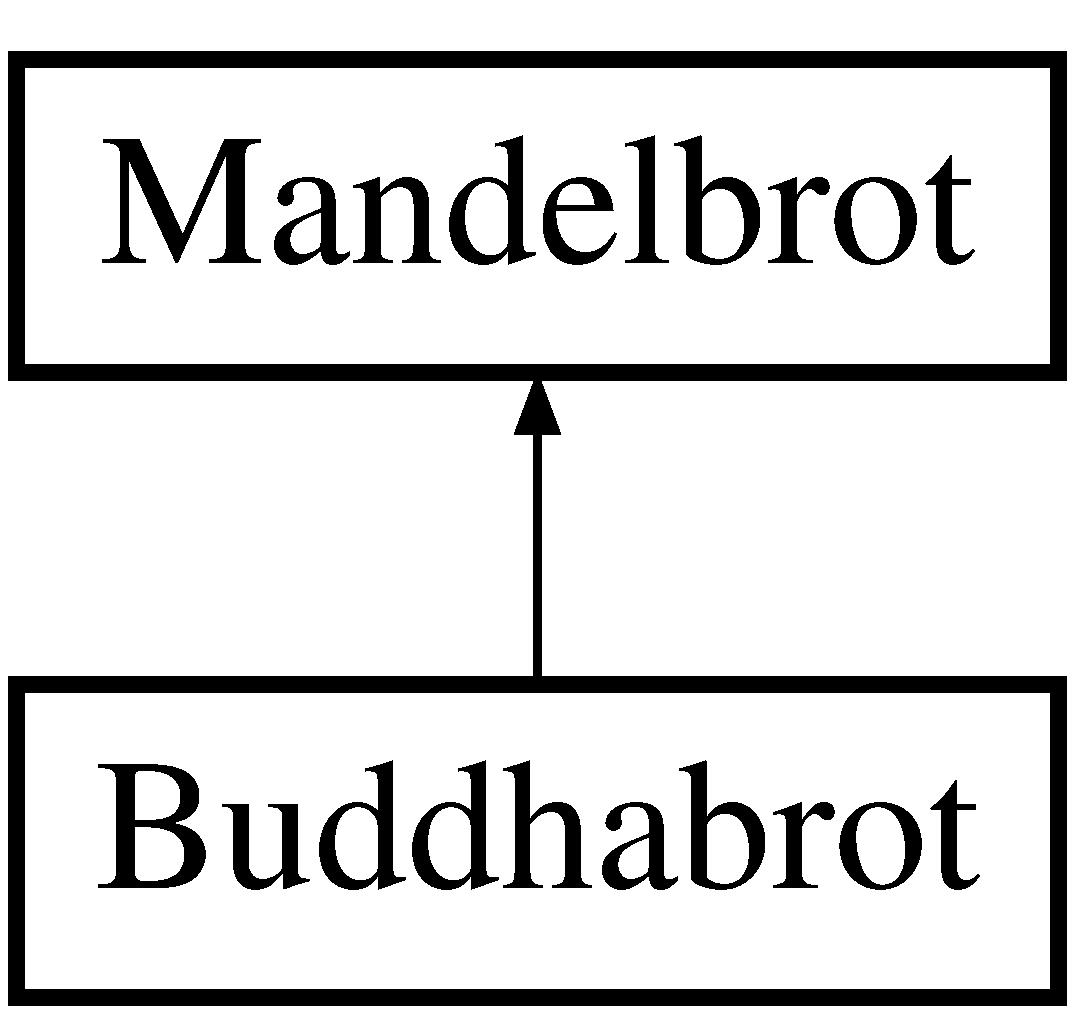
\includegraphics[height=2.000000cm]{class_buddhabrot}
\end{center}
\end{figure}
\subsection*{Public Member Functions}
\begin{DoxyCompactItemize}
\item 
\hyperlink{class_buddhabrot_a3785536aee5b43aac307c8c737d0a1bb}{Buddhabrot} (unsigned threads, unsigned depth)
\begin{DoxyCompactList}\small\item\em Explicitly construct a \hyperlink{class_buddhabrot}{Buddhabrot} object. \end{DoxyCompactList}\item 
\hyperlink{class_buddhabrot_ad54bede3c44cc5d9181bd6a28feb0dbd}{$\sim$\+Buddhabrot} ()
\begin{DoxyCompactList}\small\item\em Destroys a \hyperlink{class_buddhabrot}{Buddhabrot} object. \end{DoxyCompactList}\item 
void \hyperlink{class_buddhabrot_a9e65eb7e2cac8737aedec56a7e2c274c}{draw} (\hyperlink{classtsgl_1_1_cartesian_canvas}{Cart} \&can)
\begin{DoxyCompactList}\small\item\em Draw the \hyperlink{class_buddhabrot}{Buddhabrot}. \end{DoxyCompactList}\end{DoxyCompactItemize}
\subsection*{Additional Inherited Members}


\subsection{Detailed Description}
Draw a \hyperlink{class_buddhabrot}{Buddhabrot}. 

Contains all of the information necessary in order to draw a \hyperlink{class_buddhabrot}{Buddhabrot}.

Child class of the \hyperlink{class_mandelbrot}{Mandelbrot} class. \begin{DoxySeeAlso}{See also}
\href{https://en.wikipedia.org/wiki/Buddhabrot}{\tt https\+://en.\+wikipedia.\+org/wiki/\+Buddhabrot} for details on what a \hyperlink{class_buddhabrot}{Buddhabrot} is. 

\hyperlink{class_mandelbrot}{Mandelbrot} class 
\end{DoxySeeAlso}


\subsection{Constructor \& Destructor Documentation}
\mbox{\Hypertarget{class_buddhabrot_a3785536aee5b43aac307c8c737d0a1bb}\label{class_buddhabrot_a3785536aee5b43aac307c8c737d0a1bb}} 
\index{Buddhabrot@{Buddhabrot}!Buddhabrot@{Buddhabrot}}
\index{Buddhabrot@{Buddhabrot}!Buddhabrot@{Buddhabrot}}
\subsubsection{\texorpdfstring{Buddhabrot()}{Buddhabrot()}}
{\footnotesize\ttfamily Buddhabrot\+::\+Buddhabrot (\begin{DoxyParamCaption}\item[{unsigned}]{threads,  }\item[{unsigned}]{depth = {\ttfamily 1000} }\end{DoxyParamCaption})}



Explicitly construct a \hyperlink{class_buddhabrot}{Buddhabrot} object. 

Explicit constructor for the \hyperlink{class_buddhabrot}{Buddhabrot} class. 
\begin{DoxyParams}{Parameters}
{\em threads} & The number of threads to use when drawing the \hyperlink{class_buddhabrot}{Buddhabrot} object to the Cartesian\+Canvas. \\
\hline
{\em depth} & The number of iterations to go to in order to draw the \hyperlink{class_buddhabrot}{Buddhabrot} object. \\
\hline
\end{DoxyParams}
\begin{DoxyReturn}{Returns}
The constructed \hyperlink{class_buddhabrot}{Buddhabrot} object. 
\end{DoxyReturn}
\mbox{\Hypertarget{class_buddhabrot_ad54bede3c44cc5d9181bd6a28feb0dbd}\label{class_buddhabrot_ad54bede3c44cc5d9181bd6a28feb0dbd}} 
\index{Buddhabrot@{Buddhabrot}!````~Buddhabrot@{$\sim$\+Buddhabrot}}
\index{````~Buddhabrot@{$\sim$\+Buddhabrot}!Buddhabrot@{Buddhabrot}}
\subsubsection{\texorpdfstring{$\sim$\+Buddhabrot()}{~Buddhabrot()}}
{\footnotesize\ttfamily Buddhabrot\+::$\sim$\+Buddhabrot (\begin{DoxyParamCaption}{ }\end{DoxyParamCaption})}



Destroys a \hyperlink{class_buddhabrot}{Buddhabrot} object. 

Destructor for the \hyperlink{class_buddhabrot}{Buddhabrot} class. \begin{DoxyReturn}{Returns}
Frees up memory allocated to a \hyperlink{class_buddhabrot}{Buddhabrot} object. 
\end{DoxyReturn}


\subsection{Member Function Documentation}
\mbox{\Hypertarget{class_buddhabrot_a9e65eb7e2cac8737aedec56a7e2c274c}\label{class_buddhabrot_a9e65eb7e2cac8737aedec56a7e2c274c}} 
\index{Buddhabrot@{Buddhabrot}!draw@{draw}}
\index{draw@{draw}!Buddhabrot@{Buddhabrot}}
\subsubsection{\texorpdfstring{draw()}{draw()}}
{\footnotesize\ttfamily void Buddhabrot\+::draw (\begin{DoxyParamCaption}\item[{\hyperlink{classtsgl_1_1_cartesian_canvas}{Cart} \&}]{can }\end{DoxyParamCaption})\hspace{0.3cm}{\ttfamily [virtual]}}



Draw the \hyperlink{class_buddhabrot}{Buddhabrot}. 

Actually draws the \hyperlink{class_buddhabrot}{Buddhabrot} object to the Cartesian\+Canvas. 
\begin{DoxyParams}{Parameters}
{\em can} & Reference to the Cartesian\+Canvas to draw on. \\
\hline
\end{DoxyParams}
\begin{DoxyNote}{Note}
This method overrides the \hyperlink{class_buddhabrot_a9e65eb7e2cac8737aedec56a7e2c274c}{draw()} method from \hyperlink{class_mandelbrot}{Mandelbrot}. 

Cart is a typedef for Cartesian\+Canvas. 
\end{DoxyNote}


Reimplemented from \hyperlink{class_mandelbrot_ab7918e4de8f00f73290f110ca7a6cffd}{Mandelbrot}.



The documentation for this class was generated from the following files\+:\begin{DoxyCompactItemize}
\item 
/home/sth5/test/\+T\+S\+G\+L/src/examples/\+Mandelbrot/Buddhabrot.\+h\item 
/home/sth5/test/\+T\+S\+G\+L/src/examples/\+Mandelbrot/Buddhabrot.\+cpp\end{DoxyCompactItemize}

\hypertarget{classtsgl_1_1_camera}{}\section{tsgl\+:\+:Camera Class Reference}
\label{classtsgl_1_1_camera}\index{tsgl\+::\+Camera@{tsgl\+::\+Camera}}


Defines a movable, rotatable camera-\/like object and its corresponding view matrix.  




{\ttfamily \#include $<$Camera.\+h$>$}

\subsection*{Public Member Functions}
\begin{DoxyCompactItemize}
\item 
\hyperlink{classtsgl_1_1_camera_ad55c777a783afe64666b22c4867a2ac0}{Camera} (glm\+::vec3 position, glm\+::vec3 up, glm\+::vec3 target)
\begin{DoxyCompactList}\small\item\em Explicitly constructs a new \hyperlink{classtsgl_1_1_camera}{Camera}. \end{DoxyCompactList}\item 
\hyperlink{classtsgl_1_1_camera_a3024adf593e6097eff73152305af9dee}{Camera} (float posX, float posY, float posZ, float upX, float upY, float upZ, float targetX, float targetY, float targetZ)
\begin{DoxyCompactList}\small\item\em Explicitly constructs a new \hyperlink{classtsgl_1_1_camera}{Camera}. \end{DoxyCompactList}\item 
\hyperlink{classtsgl_1_1_camera_a19bf2769862005ac36d7bacce3ec8400}{Camera} (glm\+::vec3 position, glm\+::vec3 up, float yaw, float pitch)
\begin{DoxyCompactList}\small\item\em Explicitly constructs a new \hyperlink{classtsgl_1_1_camera}{Camera}. \end{DoxyCompactList}\item 
\hyperlink{classtsgl_1_1_camera_ad4263c9f9805ab92dd3996a2738dad8b}{Camera} (float posX, float posY, float posZ, float upX, float upY, float upZ, float yaw, float pitch)
\begin{DoxyCompactList}\small\item\em Explicitly constructs a new \hyperlink{classtsgl_1_1_camera}{Camera}. \end{DoxyCompactList}\item 
glm\+::mat4 \hyperlink{classtsgl_1_1_camera_acb98691025f9ea89b63b06ee184409b4}{get\+View\+Matrix} ()
\begin{DoxyCompactList}\small\item\em Accessor for the corresponding view matrix for the \hyperlink{classtsgl_1_1_camera}{Camera}. \end{DoxyCompactList}\item 
void \hyperlink{classtsgl_1_1_camera_a011b8c82aff7e98b7c41aa6998006c56}{change\+X\+By} (float delta)
\begin{DoxyCompactList}\small\item\em Mutator for \hyperlink{classtsgl_1_1_camera}{Camera}\textquotesingle{}s x-\/coordinate in world space. \end{DoxyCompactList}\item 
void \hyperlink{classtsgl_1_1_camera_a9d6f2bd303dfd57068cbb35b4be0e78c}{change\+Y\+By} (float delta)
\begin{DoxyCompactList}\small\item\em Mutator for \hyperlink{classtsgl_1_1_camera}{Camera}\textquotesingle{}s y-\/coordinate in world space. \end{DoxyCompactList}\item 
void \hyperlink{classtsgl_1_1_camera_ab9aa61c8939c23f31801028adc0b5b4d}{change\+Z\+By} (float delta)
\begin{DoxyCompactList}\small\item\em Mutator for \hyperlink{classtsgl_1_1_camera}{Camera}\textquotesingle{}s z-\/coordinate in world space. \end{DoxyCompactList}\item 
void \hyperlink{classtsgl_1_1_camera_adda85f9211c54d33584cee240ed0ec47}{move\+Backward} (float delta)
\begin{DoxyCompactList}\small\item\em Moves the \hyperlink{classtsgl_1_1_camera}{Camera} backward, relative to its orientation, by delta. \end{DoxyCompactList}\item 
void \hyperlink{classtsgl_1_1_camera_a9f8d73bb09703cfe3e46dea725dca49a}{move\+Forward} (float delta)
\begin{DoxyCompactList}\small\item\em Moves the \hyperlink{classtsgl_1_1_camera}{Camera} forward, relative to its orientation, by delta. \end{DoxyCompactList}\item 
void \hyperlink{classtsgl_1_1_camera_ac672a6337590083e320be253bfe38ba1}{move\+Down} (float delta)
\begin{DoxyCompactList}\small\item\em Moves the \hyperlink{classtsgl_1_1_camera}{Camera} downward, relative to its orientation, by delta. \end{DoxyCompactList}\item 
void \hyperlink{classtsgl_1_1_camera_a60a565d006b727c305567d36b13e6e08}{move\+Up} (float delta)
\begin{DoxyCompactList}\small\item\em Moves the \hyperlink{classtsgl_1_1_camera}{Camera} upward, relative to its orientation, by delta. \end{DoxyCompactList}\item 
void \hyperlink{classtsgl_1_1_camera_a9cd60e2a3e521263a548700d08c73cb3}{move\+Left} (float delta)
\begin{DoxyCompactList}\small\item\em Moves the \hyperlink{classtsgl_1_1_camera}{Camera} left, relative to its orientation, by delta. \end{DoxyCompactList}\item 
void \hyperlink{classtsgl_1_1_camera_ab69a0968bb1076b9303c6d10c07bbd75}{move\+Right} (float delta)
\begin{DoxyCompactList}\small\item\em Moves the \hyperlink{classtsgl_1_1_camera}{Camera} right, relative to its orientation, by delta. \end{DoxyCompactList}\item 
void \hyperlink{classtsgl_1_1_camera_aeb5d5fb50a80951a307b03d66e56eb17}{set\+Position} (glm\+::vec3 pos)
\begin{DoxyCompactList}\small\item\em Alters the \hyperlink{classtsgl_1_1_camera}{Camera}\textquotesingle{}s position in world space. \end{DoxyCompactList}\item 
void \hyperlink{classtsgl_1_1_camera_a6cb0b89abb559c839616c554554adfb4}{set\+Position} (float x, float y, float z)
\begin{DoxyCompactList}\small\item\em Alters the \hyperlink{classtsgl_1_1_camera}{Camera}\textquotesingle{}s position in world space. \end{DoxyCompactList}\item 
void \hyperlink{classtsgl_1_1_camera_a928177f16143b27b88de7ecf30d797ae}{set\+PositionX} (float x)
\begin{DoxyCompactList}\small\item\em Sets the \hyperlink{classtsgl_1_1_camera}{Camera}\textquotesingle{}s x-\/coordinate in world space. \end{DoxyCompactList}\item 
void \hyperlink{classtsgl_1_1_camera_aa4b72d96ba1d802c6940fdd8f9f7f472}{set\+PositionY} (float y)
\begin{DoxyCompactList}\small\item\em Sets the \hyperlink{classtsgl_1_1_camera}{Camera}\textquotesingle{}s y-\/coordinate co in world space. \end{DoxyCompactList}\item 
void \hyperlink{classtsgl_1_1_camera_a87c83395dbde5a8fce49cba5200a0a5c}{set\+PositionZ} (float z)
\begin{DoxyCompactList}\small\item\em Sets the \hyperlink{classtsgl_1_1_camera}{Camera}\textquotesingle{}s z-\/coordinate in world space. \end{DoxyCompactList}\item 
void \hyperlink{classtsgl_1_1_camera_a3228e5545b7f20bc39282ea9267acfda}{look\+At} (float x, float y, float z)
\begin{DoxyCompactList}\small\item\em Alters the point at which the \hyperlink{classtsgl_1_1_camera}{Camera} looks in world space. \end{DoxyCompactList}\item 
void \hyperlink{classtsgl_1_1_camera_ade60f005d962cde8397ea080251eba93}{change\+Yaw\+By} (float delta)
\begin{DoxyCompactList}\small\item\em Alters the \hyperlink{classtsgl_1_1_camera}{Camera}\textquotesingle{}s yaw rotation. \end{DoxyCompactList}\item 
void \hyperlink{classtsgl_1_1_camera_af8df38d9efb33604af16c13e2a8446e0}{change\+Pitch\+By} (float delta)
\begin{DoxyCompactList}\small\item\em Alters the \hyperlink{classtsgl_1_1_camera}{Camera}\textquotesingle{}s pitch rotation. \end{DoxyCompactList}\item 
float \hyperlink{classtsgl_1_1_camera_a73756ae570553923c70a084c11f1d225}{get\+Pitch} ()
\begin{DoxyCompactList}\small\item\em Accessor for the \hyperlink{classtsgl_1_1_camera}{Camera}\textquotesingle{}s pitch. \end{DoxyCompactList}\item 
float \hyperlink{classtsgl_1_1_camera_ae66ea7ccf619657cf817e70c934a3d36}{get\+Yaw} ()
\begin{DoxyCompactList}\small\item\em Accessor for the \hyperlink{classtsgl_1_1_camera}{Camera}\textquotesingle{}s yaw. \end{DoxyCompactList}\item 
glm\+::vec3 \hyperlink{classtsgl_1_1_camera_a21d2c903c077e9a746cd150e2e2bc697}{get\+Position} ()
\begin{DoxyCompactList}\small\item\em Accessor for the \hyperlink{classtsgl_1_1_camera}{Camera}\textquotesingle{}s position in world space. \end{DoxyCompactList}\item 
float \hyperlink{classtsgl_1_1_camera_abd7723919bb264f1e4a9fd666a280c8d}{get\+PositionX} ()
\begin{DoxyCompactList}\small\item\em Accessor for the x-\/coordinate of the \hyperlink{classtsgl_1_1_camera}{Camera}\textquotesingle{}s position in world space. \end{DoxyCompactList}\item 
float \hyperlink{classtsgl_1_1_camera_a14bb7fed2c2772b927dcd9f37807201e}{get\+PositionY} ()
\begin{DoxyCompactList}\small\item\em Accessor for the y-\/coordinate of the \hyperlink{classtsgl_1_1_camera}{Camera}\textquotesingle{}s position in world space. \end{DoxyCompactList}\item 
float \hyperlink{classtsgl_1_1_camera_a73a1acb7ff3a1166e2d6a4be16874219}{get\+PositionZ} ()
\begin{DoxyCompactList}\small\item\em Accessor for the z-\/coordinate of the \hyperlink{classtsgl_1_1_camera}{Camera}\textquotesingle{}s position in world space. \end{DoxyCompactList}\item 
glm\+::vec3 \hyperlink{classtsgl_1_1_camera_a8c6c19acef5dffc6dfc2aff31428d2e1}{get\+Target} ()
\begin{DoxyCompactList}\small\item\em Accessor for the point at which \hyperlink{classtsgl_1_1_camera}{Camera} looks in world space. \end{DoxyCompactList}\item 
float \hyperlink{classtsgl_1_1_camera_ad5778df0178d7926bdb2da22556b03b0}{get\+TargetX} ()
\begin{DoxyCompactList}\small\item\em Accessor for the x-\/coordinate of the point at which \hyperlink{classtsgl_1_1_camera}{Camera} looks in world space. \end{DoxyCompactList}\item 
float \hyperlink{classtsgl_1_1_camera_ac06e3f420e82af5189f525881191031b}{get\+TargetY} ()
\begin{DoxyCompactList}\small\item\em Accessor for the y-\/coordinate of the point at which \hyperlink{classtsgl_1_1_camera}{Camera} looks in world space. \end{DoxyCompactList}\item 
float \hyperlink{classtsgl_1_1_camera_a1ceef7ca9535c701c7c70741c1170dea}{get\+TargetZ} ()
\begin{DoxyCompactList}\small\item\em Accessor for the z-\/coordinate of the point at which \hyperlink{classtsgl_1_1_camera}{Camera} looks in world space. \end{DoxyCompactList}\end{DoxyCompactItemize}
\subsection*{Protected Member Functions}
\begin{DoxyCompactItemize}
\item 
void \hyperlink{classtsgl_1_1_camera_ac2daf561e3b110fe4ec17b23e530c01e}{update\+Camera\+Angle} ()
\begin{DoxyCompactList}\small\item\em Protected helper method that recalculates \hyperlink{classtsgl_1_1_camera}{Camera}\textquotesingle{}s my\+Front vector based on yaw and pitch. \end{DoxyCompactList}\end{DoxyCompactItemize}
\subsection*{Protected Attributes}
\begin{DoxyCompactItemize}
\item 
\mbox{\Hypertarget{classtsgl_1_1_camera_ac8e69c5f97e19905b09b01c0bf876274}\label{classtsgl_1_1_camera_ac8e69c5f97e19905b09b01c0bf876274}} 
glm\+::vec3 {\bfseries my\+Position}
\item 
\mbox{\Hypertarget{classtsgl_1_1_camera_a04dcfb1e8061ac4cf4b4ebb79ba1b5b0}\label{classtsgl_1_1_camera_a04dcfb1e8061ac4cf4b4ebb79ba1b5b0}} 
glm\+::vec3 {\bfseries my\+Front}
\item 
\mbox{\Hypertarget{classtsgl_1_1_camera_a433e056f81c1b6488fed8fb314e2ea84}\label{classtsgl_1_1_camera_a433e056f81c1b6488fed8fb314e2ea84}} 
glm\+::vec3 {\bfseries my\+Up}
\item 
\mbox{\Hypertarget{classtsgl_1_1_camera_aaf772a056a8c2e64056583158b472a38}\label{classtsgl_1_1_camera_aaf772a056a8c2e64056583158b472a38}} 
glm\+::vec3 {\bfseries my\+Right}
\item 
\mbox{\Hypertarget{classtsgl_1_1_camera_a7da972a788e67ccbddb210aaafa05584}\label{classtsgl_1_1_camera_a7da972a788e67ccbddb210aaafa05584}} 
glm\+::vec3 {\bfseries my\+World\+Up}
\item 
\mbox{\Hypertarget{classtsgl_1_1_camera_adf4f3c5959cda3bb47e7f20fcaca19a5}\label{classtsgl_1_1_camera_adf4f3c5959cda3bb47e7f20fcaca19a5}} 
float {\bfseries my\+Yaw}
\item 
\mbox{\Hypertarget{classtsgl_1_1_camera_a037f7d3e8d5ddefe92e2d221fd585432}\label{classtsgl_1_1_camera_a037f7d3e8d5ddefe92e2d221fd585432}} 
float {\bfseries my\+Pitch}
\item 
\mbox{\Hypertarget{classtsgl_1_1_camera_aa1b04e1f336367fed432b50a2539f4e5}\label{classtsgl_1_1_camera_aa1b04e1f336367fed432b50a2539f4e5}} 
std\+::mutex {\bfseries attrib\+Mutex}
\end{DoxyCompactItemize}


\subsection{Detailed Description}
Defines a movable, rotatable camera-\/like object and its corresponding view matrix. 

\hyperlink{classtsgl_1_1_camera}{Camera} is used within T\+S\+G\+L\+::\+Canvas to define the view matrix. 

\subsection{Constructor \& Destructor Documentation}
\mbox{\Hypertarget{classtsgl_1_1_camera_ad55c777a783afe64666b22c4867a2ac0}\label{classtsgl_1_1_camera_ad55c777a783afe64666b22c4867a2ac0}} 
\index{tsgl\+::\+Camera@{tsgl\+::\+Camera}!Camera@{Camera}}
\index{Camera@{Camera}!tsgl\+::\+Camera@{tsgl\+::\+Camera}}
\subsubsection{\texorpdfstring{Camera()}{Camera()}\hspace{0.1cm}{\footnotesize\ttfamily [1/4]}}
{\footnotesize\ttfamily tsgl\+::\+Camera\+::\+Camera (\begin{DoxyParamCaption}\item[{glm\+::vec3}]{position,  }\item[{glm\+::vec3}]{up,  }\item[{glm\+::vec3}]{target }\end{DoxyParamCaption})}



Explicitly constructs a new \hyperlink{classtsgl_1_1_camera}{Camera}. 

Explicit constructor for a \hyperlink{classtsgl_1_1_camera}{Camera} object. 
\begin{DoxyParams}{Parameters}
{\em position} & The \hyperlink{classtsgl_1_1_camera}{Camera}\textquotesingle{}s location in 3D space, a glm\+::vec3. \\
\hline
{\em up} & A 3D vector indicating the up direction in world space. \\
\hline
{\em target} & The point at which the \hyperlink{classtsgl_1_1_camera}{Camera} will look. \\
\hline
\end{DoxyParams}
\begin{DoxyReturn}{Returns}
A new \hyperlink{classtsgl_1_1_camera}{Camera} object, used to represent and return a corresponding view matrix. 
\end{DoxyReturn}
\mbox{\Hypertarget{classtsgl_1_1_camera_a3024adf593e6097eff73152305af9dee}\label{classtsgl_1_1_camera_a3024adf593e6097eff73152305af9dee}} 
\index{tsgl\+::\+Camera@{tsgl\+::\+Camera}!Camera@{Camera}}
\index{Camera@{Camera}!tsgl\+::\+Camera@{tsgl\+::\+Camera}}
\subsubsection{\texorpdfstring{Camera()}{Camera()}\hspace{0.1cm}{\footnotesize\ttfamily [2/4]}}
{\footnotesize\ttfamily tsgl\+::\+Camera\+::\+Camera (\begin{DoxyParamCaption}\item[{float}]{posX,  }\item[{float}]{posY,  }\item[{float}]{posZ,  }\item[{float}]{upX,  }\item[{float}]{upY,  }\item[{float}]{upZ,  }\item[{float}]{targetX,  }\item[{float}]{targetY,  }\item[{float}]{targetZ }\end{DoxyParamCaption})}



Explicitly constructs a new \hyperlink{classtsgl_1_1_camera}{Camera}. 

Explicit constructor for a \hyperlink{classtsgl_1_1_camera}{Camera} object. 
\begin{DoxyParams}{Parameters}
{\em posX} & The \hyperlink{classtsgl_1_1_camera}{Camera}\textquotesingle{}s positional x-\/coordinate in 3D space, a float. \\
\hline
{\em posY} & The \hyperlink{classtsgl_1_1_camera}{Camera}\textquotesingle{}s positional y-\/coordinate in 3D space, a float. \\
\hline
{\em posZ} & The \hyperlink{classtsgl_1_1_camera}{Camera}\textquotesingle{}s positional z-\/coordinate in 3D space, a float. \\
\hline
{\em upX} & The x-\/component of a 3D vector indicating the up direction in world space. \\
\hline
{\em upY} & The y-\/component of a 3D vector indicating the up direction in world space. \\
\hline
{\em upZ} & The z-\/component of a 3D vector indicating the up direction in world space. \\
\hline
{\em targetX} & The x-\/coordinate of the point at which the \hyperlink{classtsgl_1_1_camera}{Camera} will look. \\
\hline
{\em targetY} & The y-\/coordinate of the point at which the \hyperlink{classtsgl_1_1_camera}{Camera} will look. \\
\hline
{\em targetZ} & The z-\/coordinate of the point at which the \hyperlink{classtsgl_1_1_camera}{Camera} will look. \\
\hline
\end{DoxyParams}
\begin{DoxyReturn}{Returns}
A new \hyperlink{classtsgl_1_1_camera}{Camera} object, used to represent and return a corresponding view matrix. 
\end{DoxyReturn}
\mbox{\Hypertarget{classtsgl_1_1_camera_a19bf2769862005ac36d7bacce3ec8400}\label{classtsgl_1_1_camera_a19bf2769862005ac36d7bacce3ec8400}} 
\index{tsgl\+::\+Camera@{tsgl\+::\+Camera}!Camera@{Camera}}
\index{Camera@{Camera}!tsgl\+::\+Camera@{tsgl\+::\+Camera}}
\subsubsection{\texorpdfstring{Camera()}{Camera()}\hspace{0.1cm}{\footnotesize\ttfamily [3/4]}}
{\footnotesize\ttfamily tsgl\+::\+Camera\+::\+Camera (\begin{DoxyParamCaption}\item[{glm\+::vec3}]{position,  }\item[{glm\+::vec3}]{up,  }\item[{float}]{yaw,  }\item[{float}]{pitch }\end{DoxyParamCaption})}



Explicitly constructs a new \hyperlink{classtsgl_1_1_camera}{Camera}. 

Explicit constructor for a \hyperlink{classtsgl_1_1_camera}{Camera} object. 
\begin{DoxyParams}{Parameters}
{\em position} & The \hyperlink{classtsgl_1_1_camera}{Camera}\textquotesingle{}s location in 3D space, a glm\+::vec3. \\
\hline
{\em up} & A 3D vector indicating the up direction in world space. \\
\hline
{\em yaw} & The camera\textquotesingle{}s yaw rotation (horizontal) in degrees. \\
\hline
{\em pitch} & The camera\textquotesingle{}s pitch rotation (vertical) in degrees. \\
\hline
\end{DoxyParams}
\begin{DoxyNote}{Note}
With position.\+x and position.\+y equal to 0 and a positive position.\+z, a yaw of -\/90 degrees and pitch of 0 degrees will look at (0,0,0). 

pitch is constrained between -\/89 and 89 degrees. 
\end{DoxyNote}
\begin{DoxyReturn}{Returns}
A new \hyperlink{classtsgl_1_1_camera}{Camera} object, used to represent and return a corresponding view matrix. 
\end{DoxyReturn}
\mbox{\Hypertarget{classtsgl_1_1_camera_ad4263c9f9805ab92dd3996a2738dad8b}\label{classtsgl_1_1_camera_ad4263c9f9805ab92dd3996a2738dad8b}} 
\index{tsgl\+::\+Camera@{tsgl\+::\+Camera}!Camera@{Camera}}
\index{Camera@{Camera}!tsgl\+::\+Camera@{tsgl\+::\+Camera}}
\subsubsection{\texorpdfstring{Camera()}{Camera()}\hspace{0.1cm}{\footnotesize\ttfamily [4/4]}}
{\footnotesize\ttfamily tsgl\+::\+Camera\+::\+Camera (\begin{DoxyParamCaption}\item[{float}]{posX,  }\item[{float}]{posY,  }\item[{float}]{posZ,  }\item[{float}]{upX,  }\item[{float}]{upY,  }\item[{float}]{upZ,  }\item[{float}]{yaw,  }\item[{float}]{pitch }\end{DoxyParamCaption})}



Explicitly constructs a new \hyperlink{classtsgl_1_1_camera}{Camera}. 

Explicit constructor for a \hyperlink{classtsgl_1_1_camera}{Camera} object. 
\begin{DoxyParams}{Parameters}
{\em posX} & The \hyperlink{classtsgl_1_1_camera}{Camera}\textquotesingle{}s positional x-\/coordinate in 3D space, a float. \\
\hline
{\em posY} & The \hyperlink{classtsgl_1_1_camera}{Camera}\textquotesingle{}s positional y-\/coordinate in 3D space, a float. \\
\hline
{\em posZ} & The \hyperlink{classtsgl_1_1_camera}{Camera}\textquotesingle{}s positional z-\/coordinate in 3D space, a float. \\
\hline
{\em upX} & The x-\/component of a 3D vector indicating the up direction in world space. \\
\hline
{\em upY} & The y-\/component of a 3D vector indicating the up direction in world space. \\
\hline
{\em upZ} & The z-\/component of a 3D vector indicating the up direction in world space. \\
\hline
{\em yaw} & The camera\textquotesingle{}s yaw rotation (horizontal) in degrees. \\
\hline
{\em pitch} & The camera\textquotesingle{}s pitch rotation (vertical) in degrees. \\
\hline
\end{DoxyParams}
\begin{DoxyNote}{Note}
With posX and posY equal to 0 and a positive posZ, a yaw of -\/90 degrees and pitch of 0 degrees will look at (0,0,0). 

pitch is constrained between -\/89 and 89 degrees. 
\end{DoxyNote}
\begin{DoxyReturn}{Returns}
A new \hyperlink{classtsgl_1_1_camera}{Camera} object, used to represent and return a corresponding view matrix. 
\end{DoxyReturn}


\subsection{Member Function Documentation}
\mbox{\Hypertarget{classtsgl_1_1_camera_af8df38d9efb33604af16c13e2a8446e0}\label{classtsgl_1_1_camera_af8df38d9efb33604af16c13e2a8446e0}} 
\index{tsgl\+::\+Camera@{tsgl\+::\+Camera}!change\+Pitch\+By@{change\+Pitch\+By}}
\index{change\+Pitch\+By@{change\+Pitch\+By}!tsgl\+::\+Camera@{tsgl\+::\+Camera}}
\subsubsection{\texorpdfstring{change\+Pitch\+By()}{changePitchBy()}}
{\footnotesize\ttfamily void tsgl\+::\+Camera\+::change\+Pitch\+By (\begin{DoxyParamCaption}\item[{float}]{delta }\end{DoxyParamCaption})}



Alters the \hyperlink{classtsgl_1_1_camera}{Camera}\textquotesingle{}s pitch rotation. 

Based on the original direction the \hyperlink{classtsgl_1_1_camera}{Camera} was set to face, the \hyperlink{classtsgl_1_1_camera}{Camera} is rotated according to the parameter. 
\begin{DoxyParams}{Parameters}
{\em delta} & The amount by which to change the \hyperlink{classtsgl_1_1_camera}{Camera}\textquotesingle{}s pitch, in degrees. \\
\hline
\end{DoxyParams}
\begin{DoxyNote}{Note}
pitch is constrained between -\/89 and 89 degrees. 
\end{DoxyNote}
\mbox{\Hypertarget{classtsgl_1_1_camera_a011b8c82aff7e98b7c41aa6998006c56}\label{classtsgl_1_1_camera_a011b8c82aff7e98b7c41aa6998006c56}} 
\index{tsgl\+::\+Camera@{tsgl\+::\+Camera}!change\+X\+By@{change\+X\+By}}
\index{change\+X\+By@{change\+X\+By}!tsgl\+::\+Camera@{tsgl\+::\+Camera}}
\subsubsection{\texorpdfstring{change\+X\+By()}{changeXBy()}}
{\footnotesize\ttfamily void tsgl\+::\+Camera\+::change\+X\+By (\begin{DoxyParamCaption}\item[{float}]{delta }\end{DoxyParamCaption})}



Mutator for \hyperlink{classtsgl_1_1_camera}{Camera}\textquotesingle{}s x-\/coordinate in world space. 

Alters the x component of \hyperlink{classtsgl_1_1_camera}{Camera}\textquotesingle{}s my\+Position vector by delta. 
\begin{DoxyParams}{Parameters}
{\em delta} & The difference between camera\textquotesingle{}s new and old x-\/coordinates. \\
\hline
\end{DoxyParams}
\mbox{\Hypertarget{classtsgl_1_1_camera_ade60f005d962cde8397ea080251eba93}\label{classtsgl_1_1_camera_ade60f005d962cde8397ea080251eba93}} 
\index{tsgl\+::\+Camera@{tsgl\+::\+Camera}!change\+Yaw\+By@{change\+Yaw\+By}}
\index{change\+Yaw\+By@{change\+Yaw\+By}!tsgl\+::\+Camera@{tsgl\+::\+Camera}}
\subsubsection{\texorpdfstring{change\+Yaw\+By()}{changeYawBy()}}
{\footnotesize\ttfamily void tsgl\+::\+Camera\+::change\+Yaw\+By (\begin{DoxyParamCaption}\item[{float}]{delta }\end{DoxyParamCaption})}



Alters the \hyperlink{classtsgl_1_1_camera}{Camera}\textquotesingle{}s yaw rotation. 

Based on the original direction the \hyperlink{classtsgl_1_1_camera}{Camera} was set to face, the \hyperlink{classtsgl_1_1_camera}{Camera} is rotated according to the parameter. 
\begin{DoxyParams}{Parameters}
{\em delta} & The amount by which to change the \hyperlink{classtsgl_1_1_camera}{Camera}\textquotesingle{}s yaw, in degrees. \\
\hline
\end{DoxyParams}
\mbox{\Hypertarget{classtsgl_1_1_camera_a9d6f2bd303dfd57068cbb35b4be0e78c}\label{classtsgl_1_1_camera_a9d6f2bd303dfd57068cbb35b4be0e78c}} 
\index{tsgl\+::\+Camera@{tsgl\+::\+Camera}!change\+Y\+By@{change\+Y\+By}}
\index{change\+Y\+By@{change\+Y\+By}!tsgl\+::\+Camera@{tsgl\+::\+Camera}}
\subsubsection{\texorpdfstring{change\+Y\+By()}{changeYBy()}}
{\footnotesize\ttfamily void tsgl\+::\+Camera\+::change\+Y\+By (\begin{DoxyParamCaption}\item[{float}]{delta }\end{DoxyParamCaption})}



Mutator for \hyperlink{classtsgl_1_1_camera}{Camera}\textquotesingle{}s y-\/coordinate in world space. 

Alters the y component of \hyperlink{classtsgl_1_1_camera}{Camera}\textquotesingle{}s my\+Position vector by delta. 
\begin{DoxyParams}{Parameters}
{\em delta} & The difference between camera\textquotesingle{}s new and old y-\/coordinates. \\
\hline
\end{DoxyParams}
\mbox{\Hypertarget{classtsgl_1_1_camera_ab9aa61c8939c23f31801028adc0b5b4d}\label{classtsgl_1_1_camera_ab9aa61c8939c23f31801028adc0b5b4d}} 
\index{tsgl\+::\+Camera@{tsgl\+::\+Camera}!change\+Z\+By@{change\+Z\+By}}
\index{change\+Z\+By@{change\+Z\+By}!tsgl\+::\+Camera@{tsgl\+::\+Camera}}
\subsubsection{\texorpdfstring{change\+Z\+By()}{changeZBy()}}
{\footnotesize\ttfamily void tsgl\+::\+Camera\+::change\+Z\+By (\begin{DoxyParamCaption}\item[{float}]{delta }\end{DoxyParamCaption})}



Mutator for \hyperlink{classtsgl_1_1_camera}{Camera}\textquotesingle{}s z-\/coordinate in world space. 

Alters the z component of \hyperlink{classtsgl_1_1_camera}{Camera}\textquotesingle{}s my\+Position vector by delta. 
\begin{DoxyParams}{Parameters}
{\em delta} & The difference between camera\textquotesingle{}s new and old z-\/coordinates. \\
\hline
\end{DoxyParams}
\mbox{\Hypertarget{classtsgl_1_1_camera_a73756ae570553923c70a084c11f1d225}\label{classtsgl_1_1_camera_a73756ae570553923c70a084c11f1d225}} 
\index{tsgl\+::\+Camera@{tsgl\+::\+Camera}!get\+Pitch@{get\+Pitch}}
\index{get\+Pitch@{get\+Pitch}!tsgl\+::\+Camera@{tsgl\+::\+Camera}}
\subsubsection{\texorpdfstring{get\+Pitch()}{getPitch()}}
{\footnotesize\ttfamily float tsgl\+::\+Camera\+::get\+Pitch (\begin{DoxyParamCaption}{ }\end{DoxyParamCaption})}



Accessor for the \hyperlink{classtsgl_1_1_camera}{Camera}\textquotesingle{}s pitch. 

Returns the value of the my\+Pitch instance variable \mbox{\Hypertarget{classtsgl_1_1_camera_a21d2c903c077e9a746cd150e2e2bc697}\label{classtsgl_1_1_camera_a21d2c903c077e9a746cd150e2e2bc697}} 
\index{tsgl\+::\+Camera@{tsgl\+::\+Camera}!get\+Position@{get\+Position}}
\index{get\+Position@{get\+Position}!tsgl\+::\+Camera@{tsgl\+::\+Camera}}
\subsubsection{\texorpdfstring{get\+Position()}{getPosition()}}
{\footnotesize\ttfamily glm\+::vec3 tsgl\+::\+Camera\+::get\+Position (\begin{DoxyParamCaption}{ }\end{DoxyParamCaption})}



Accessor for the \hyperlink{classtsgl_1_1_camera}{Camera}\textquotesingle{}s position in world space. 

Returns the value of the my\+Position instance variable \mbox{\Hypertarget{classtsgl_1_1_camera_abd7723919bb264f1e4a9fd666a280c8d}\label{classtsgl_1_1_camera_abd7723919bb264f1e4a9fd666a280c8d}} 
\index{tsgl\+::\+Camera@{tsgl\+::\+Camera}!get\+PositionX@{get\+PositionX}}
\index{get\+PositionX@{get\+PositionX}!tsgl\+::\+Camera@{tsgl\+::\+Camera}}
\subsubsection{\texorpdfstring{get\+Position\+X()}{getPositionX()}}
{\footnotesize\ttfamily float tsgl\+::\+Camera\+::get\+PositionX (\begin{DoxyParamCaption}{ }\end{DoxyParamCaption})}



Accessor for the x-\/coordinate of the \hyperlink{classtsgl_1_1_camera}{Camera}\textquotesingle{}s position in world space. 

Returns the x component of the my\+Position instance variable 

Referenced by tsgl\+::\+Canvas\+::clear\+Object\+Buffer().

\mbox{\Hypertarget{classtsgl_1_1_camera_a14bb7fed2c2772b927dcd9f37807201e}\label{classtsgl_1_1_camera_a14bb7fed2c2772b927dcd9f37807201e}} 
\index{tsgl\+::\+Camera@{tsgl\+::\+Camera}!get\+PositionY@{get\+PositionY}}
\index{get\+PositionY@{get\+PositionY}!tsgl\+::\+Camera@{tsgl\+::\+Camera}}
\subsubsection{\texorpdfstring{get\+Position\+Y()}{getPositionY()}}
{\footnotesize\ttfamily float tsgl\+::\+Camera\+::get\+PositionY (\begin{DoxyParamCaption}{ }\end{DoxyParamCaption})}



Accessor for the y-\/coordinate of the \hyperlink{classtsgl_1_1_camera}{Camera}\textquotesingle{}s position in world space. 

Returns the y component of the my\+Position instance variable 

Referenced by tsgl\+::\+Canvas\+::clear\+Object\+Buffer().

\mbox{\Hypertarget{classtsgl_1_1_camera_a73a1acb7ff3a1166e2d6a4be16874219}\label{classtsgl_1_1_camera_a73a1acb7ff3a1166e2d6a4be16874219}} 
\index{tsgl\+::\+Camera@{tsgl\+::\+Camera}!get\+PositionZ@{get\+PositionZ}}
\index{get\+PositionZ@{get\+PositionZ}!tsgl\+::\+Camera@{tsgl\+::\+Camera}}
\subsubsection{\texorpdfstring{get\+Position\+Z()}{getPositionZ()}}
{\footnotesize\ttfamily float tsgl\+::\+Camera\+::get\+PositionZ (\begin{DoxyParamCaption}{ }\end{DoxyParamCaption})}



Accessor for the z-\/coordinate of the \hyperlink{classtsgl_1_1_camera}{Camera}\textquotesingle{}s position in world space. 

Returns the z component of the my\+Position instance variable 

Referenced by tsgl\+::\+Canvas\+::clear\+Object\+Buffer().

\mbox{\Hypertarget{classtsgl_1_1_camera_a8c6c19acef5dffc6dfc2aff31428d2e1}\label{classtsgl_1_1_camera_a8c6c19acef5dffc6dfc2aff31428d2e1}} 
\index{tsgl\+::\+Camera@{tsgl\+::\+Camera}!get\+Target@{get\+Target}}
\index{get\+Target@{get\+Target}!tsgl\+::\+Camera@{tsgl\+::\+Camera}}
\subsubsection{\texorpdfstring{get\+Target()}{getTarget()}}
{\footnotesize\ttfamily glm\+::vec3 tsgl\+::\+Camera\+::get\+Target (\begin{DoxyParamCaption}{ }\end{DoxyParamCaption})}



Accessor for the point at which \hyperlink{classtsgl_1_1_camera}{Camera} looks in world space. 

Returns the sum of the my\+Position and my\+Front instance variables \mbox{\Hypertarget{classtsgl_1_1_camera_ad5778df0178d7926bdb2da22556b03b0}\label{classtsgl_1_1_camera_ad5778df0178d7926bdb2da22556b03b0}} 
\index{tsgl\+::\+Camera@{tsgl\+::\+Camera}!get\+TargetX@{get\+TargetX}}
\index{get\+TargetX@{get\+TargetX}!tsgl\+::\+Camera@{tsgl\+::\+Camera}}
\subsubsection{\texorpdfstring{get\+Target\+X()}{getTargetX()}}
{\footnotesize\ttfamily float tsgl\+::\+Camera\+::get\+TargetX (\begin{DoxyParamCaption}{ }\end{DoxyParamCaption})}



Accessor for the x-\/coordinate of the point at which \hyperlink{classtsgl_1_1_camera}{Camera} looks in world space. 

Returns the x component of the sum of the my\+Position and my\+Front instance variables \mbox{\Hypertarget{classtsgl_1_1_camera_ac06e3f420e82af5189f525881191031b}\label{classtsgl_1_1_camera_ac06e3f420e82af5189f525881191031b}} 
\index{tsgl\+::\+Camera@{tsgl\+::\+Camera}!get\+TargetY@{get\+TargetY}}
\index{get\+TargetY@{get\+TargetY}!tsgl\+::\+Camera@{tsgl\+::\+Camera}}
\subsubsection{\texorpdfstring{get\+Target\+Y()}{getTargetY()}}
{\footnotesize\ttfamily float tsgl\+::\+Camera\+::get\+TargetY (\begin{DoxyParamCaption}{ }\end{DoxyParamCaption})}



Accessor for the y-\/coordinate of the point at which \hyperlink{classtsgl_1_1_camera}{Camera} looks in world space. 

Returns the y component of the sum of the my\+Position and my\+Front instance variables \mbox{\Hypertarget{classtsgl_1_1_camera_a1ceef7ca9535c701c7c70741c1170dea}\label{classtsgl_1_1_camera_a1ceef7ca9535c701c7c70741c1170dea}} 
\index{tsgl\+::\+Camera@{tsgl\+::\+Camera}!get\+TargetZ@{get\+TargetZ}}
\index{get\+TargetZ@{get\+TargetZ}!tsgl\+::\+Camera@{tsgl\+::\+Camera}}
\subsubsection{\texorpdfstring{get\+Target\+Z()}{getTargetZ()}}
{\footnotesize\ttfamily float tsgl\+::\+Camera\+::get\+TargetZ (\begin{DoxyParamCaption}{ }\end{DoxyParamCaption})}



Accessor for the z-\/coordinate of the point at which \hyperlink{classtsgl_1_1_camera}{Camera} looks in world space. 

Returns the z component of the sum of the my\+Position and my\+Front instance variables \mbox{\Hypertarget{classtsgl_1_1_camera_acb98691025f9ea89b63b06ee184409b4}\label{classtsgl_1_1_camera_acb98691025f9ea89b63b06ee184409b4}} 
\index{tsgl\+::\+Camera@{tsgl\+::\+Camera}!get\+View\+Matrix@{get\+View\+Matrix}}
\index{get\+View\+Matrix@{get\+View\+Matrix}!tsgl\+::\+Camera@{tsgl\+::\+Camera}}
\subsubsection{\texorpdfstring{get\+View\+Matrix()}{getViewMatrix()}}
{\footnotesize\ttfamily glm\+::mat4 tsgl\+::\+Camera\+::get\+View\+Matrix (\begin{DoxyParamCaption}{ }\end{DoxyParamCaption})}



Accessor for the corresponding view matrix for the \hyperlink{classtsgl_1_1_camera}{Camera}. 

Returns a glm\+::mat4 based on \hyperlink{classtsgl_1_1_camera}{Camera}\textquotesingle{}s position and orientation. \begin{DoxyReturn}{Returns}
A glm\+::mat4 calculated by glm\+::look\+At(). 
\end{DoxyReturn}


Referenced by tsgl\+::\+Cartesian\+Background\+::select\+Shaders(), tsgl\+::\+Background\+::select\+Shaders(), tsgl\+::\+Cartesian\+Canvas\+::select\+Shaders(), and tsgl\+::\+Canvas\+::take\+Screen\+Shot().

\mbox{\Hypertarget{classtsgl_1_1_camera_ae66ea7ccf619657cf817e70c934a3d36}\label{classtsgl_1_1_camera_ae66ea7ccf619657cf817e70c934a3d36}} 
\index{tsgl\+::\+Camera@{tsgl\+::\+Camera}!get\+Yaw@{get\+Yaw}}
\index{get\+Yaw@{get\+Yaw}!tsgl\+::\+Camera@{tsgl\+::\+Camera}}
\subsubsection{\texorpdfstring{get\+Yaw()}{getYaw()}}
{\footnotesize\ttfamily float tsgl\+::\+Camera\+::get\+Yaw (\begin{DoxyParamCaption}{ }\end{DoxyParamCaption})}



Accessor for the \hyperlink{classtsgl_1_1_camera}{Camera}\textquotesingle{}s yaw. 

Returns the value of the my\+Yaw instance variable \mbox{\Hypertarget{classtsgl_1_1_camera_a3228e5545b7f20bc39282ea9267acfda}\label{classtsgl_1_1_camera_a3228e5545b7f20bc39282ea9267acfda}} 
\index{tsgl\+::\+Camera@{tsgl\+::\+Camera}!look\+At@{look\+At}}
\index{look\+At@{look\+At}!tsgl\+::\+Camera@{tsgl\+::\+Camera}}
\subsubsection{\texorpdfstring{look\+At()}{lookAt()}}
{\footnotesize\ttfamily void tsgl\+::\+Camera\+::look\+At (\begin{DoxyParamCaption}\item[{float}]{x,  }\item[{float}]{y,  }\item[{float}]{z }\end{DoxyParamCaption})}



Alters the point at which the \hyperlink{classtsgl_1_1_camera}{Camera} looks in world space. 

Sets \hyperlink{classtsgl_1_1_camera}{Camera}\textquotesingle{}s my\+Front vector, my\+Right vector, my\+Up vector, my\+Pitch, and my\+Yaw based on the parameters. 
\begin{DoxyParams}{Parameters}
{\em x} & The new x-\/coordinate at which \hyperlink{classtsgl_1_1_camera}{Camera} looks, in world space. \\
\hline
{\em y} & The new y-\/coordinate at which \hyperlink{classtsgl_1_1_camera}{Camera} looks, in world space. \\
\hline
{\em z} & The new z-\/coordinate at which \hyperlink{classtsgl_1_1_camera}{Camera} looks, in world space. \\
\hline
\end{DoxyParams}
\mbox{\Hypertarget{classtsgl_1_1_camera_adda85f9211c54d33584cee240ed0ec47}\label{classtsgl_1_1_camera_adda85f9211c54d33584cee240ed0ec47}} 
\index{tsgl\+::\+Camera@{tsgl\+::\+Camera}!move\+Backward@{move\+Backward}}
\index{move\+Backward@{move\+Backward}!tsgl\+::\+Camera@{tsgl\+::\+Camera}}
\subsubsection{\texorpdfstring{move\+Backward()}{moveBackward()}}
{\footnotesize\ttfamily void tsgl\+::\+Camera\+::move\+Backward (\begin{DoxyParamCaption}\item[{float}]{delta }\end{DoxyParamCaption})}



Moves the \hyperlink{classtsgl_1_1_camera}{Camera} backward, relative to its orientation, by delta. 

Alters \hyperlink{classtsgl_1_1_camera}{Camera}\textquotesingle{}s my\+Position vector by delta, in the opposite direction of its my\+Front vector. 
\begin{DoxyParams}{Parameters}
{\em delta} & How far backwards to move the \hyperlink{classtsgl_1_1_camera}{Camera}, in world space. \\
\hline
\end{DoxyParams}
\mbox{\Hypertarget{classtsgl_1_1_camera_ac672a6337590083e320be253bfe38ba1}\label{classtsgl_1_1_camera_ac672a6337590083e320be253bfe38ba1}} 
\index{tsgl\+::\+Camera@{tsgl\+::\+Camera}!move\+Down@{move\+Down}}
\index{move\+Down@{move\+Down}!tsgl\+::\+Camera@{tsgl\+::\+Camera}}
\subsubsection{\texorpdfstring{move\+Down()}{moveDown()}}
{\footnotesize\ttfamily void tsgl\+::\+Camera\+::move\+Down (\begin{DoxyParamCaption}\item[{float}]{delta }\end{DoxyParamCaption})}



Moves the \hyperlink{classtsgl_1_1_camera}{Camera} downward, relative to its orientation, by delta. 

Alters \hyperlink{classtsgl_1_1_camera}{Camera}\textquotesingle{}s my\+Position vector by delta, in the opposite direction of its my\+Up vector. 
\begin{DoxyParams}{Parameters}
{\em delta} & How far downward to move the \hyperlink{classtsgl_1_1_camera}{Camera}, in world space. \\
\hline
\end{DoxyParams}
\mbox{\Hypertarget{classtsgl_1_1_camera_a9f8d73bb09703cfe3e46dea725dca49a}\label{classtsgl_1_1_camera_a9f8d73bb09703cfe3e46dea725dca49a}} 
\index{tsgl\+::\+Camera@{tsgl\+::\+Camera}!move\+Forward@{move\+Forward}}
\index{move\+Forward@{move\+Forward}!tsgl\+::\+Camera@{tsgl\+::\+Camera}}
\subsubsection{\texorpdfstring{move\+Forward()}{moveForward()}}
{\footnotesize\ttfamily void tsgl\+::\+Camera\+::move\+Forward (\begin{DoxyParamCaption}\item[{float}]{delta }\end{DoxyParamCaption})}



Moves the \hyperlink{classtsgl_1_1_camera}{Camera} forward, relative to its orientation, by delta. 

Alters \hyperlink{classtsgl_1_1_camera}{Camera}\textquotesingle{}s my\+Position vector by delta, in the same direction as its my\+Front vector. 
\begin{DoxyParams}{Parameters}
{\em delta} & How far forward to move the \hyperlink{classtsgl_1_1_camera}{Camera}, in world space. \\
\hline
\end{DoxyParams}
\mbox{\Hypertarget{classtsgl_1_1_camera_a9cd60e2a3e521263a548700d08c73cb3}\label{classtsgl_1_1_camera_a9cd60e2a3e521263a548700d08c73cb3}} 
\index{tsgl\+::\+Camera@{tsgl\+::\+Camera}!move\+Left@{move\+Left}}
\index{move\+Left@{move\+Left}!tsgl\+::\+Camera@{tsgl\+::\+Camera}}
\subsubsection{\texorpdfstring{move\+Left()}{moveLeft()}}
{\footnotesize\ttfamily void tsgl\+::\+Camera\+::move\+Left (\begin{DoxyParamCaption}\item[{float}]{delta }\end{DoxyParamCaption})}



Moves the \hyperlink{classtsgl_1_1_camera}{Camera} left, relative to its orientation, by delta. 

Alters \hyperlink{classtsgl_1_1_camera}{Camera}\textquotesingle{}s my\+Position vector by delta, in the opposite direction of its my\+Right vector. 
\begin{DoxyParams}{Parameters}
{\em delta} & How far left to move the \hyperlink{classtsgl_1_1_camera}{Camera}, in world space. \\
\hline
\end{DoxyParams}
\mbox{\Hypertarget{classtsgl_1_1_camera_ab69a0968bb1076b9303c6d10c07bbd75}\label{classtsgl_1_1_camera_ab69a0968bb1076b9303c6d10c07bbd75}} 
\index{tsgl\+::\+Camera@{tsgl\+::\+Camera}!move\+Right@{move\+Right}}
\index{move\+Right@{move\+Right}!tsgl\+::\+Camera@{tsgl\+::\+Camera}}
\subsubsection{\texorpdfstring{move\+Right()}{moveRight()}}
{\footnotesize\ttfamily void tsgl\+::\+Camera\+::move\+Right (\begin{DoxyParamCaption}\item[{float}]{delta }\end{DoxyParamCaption})}



Moves the \hyperlink{classtsgl_1_1_camera}{Camera} right, relative to its orientation, by delta. 

Alters \hyperlink{classtsgl_1_1_camera}{Camera}\textquotesingle{}s my\+Position vector by delta, in the same direction as its my\+Up vector. 
\begin{DoxyParams}{Parameters}
{\em delta} & How far right to move the \hyperlink{classtsgl_1_1_camera}{Camera}, in world space. \\
\hline
\end{DoxyParams}
\mbox{\Hypertarget{classtsgl_1_1_camera_a60a565d006b727c305567d36b13e6e08}\label{classtsgl_1_1_camera_a60a565d006b727c305567d36b13e6e08}} 
\index{tsgl\+::\+Camera@{tsgl\+::\+Camera}!move\+Up@{move\+Up}}
\index{move\+Up@{move\+Up}!tsgl\+::\+Camera@{tsgl\+::\+Camera}}
\subsubsection{\texorpdfstring{move\+Up()}{moveUp()}}
{\footnotesize\ttfamily void tsgl\+::\+Camera\+::move\+Up (\begin{DoxyParamCaption}\item[{float}]{delta }\end{DoxyParamCaption})}



Moves the \hyperlink{classtsgl_1_1_camera}{Camera} upward, relative to its orientation, by delta. 

Alters \hyperlink{classtsgl_1_1_camera}{Camera}\textquotesingle{}s my\+Position vector by delta, in the same direction as its my\+Up vector. 
\begin{DoxyParams}{Parameters}
{\em delta} & How far upward to move the \hyperlink{classtsgl_1_1_camera}{Camera}, in world space. \\
\hline
\end{DoxyParams}
\mbox{\Hypertarget{classtsgl_1_1_camera_aeb5d5fb50a80951a307b03d66e56eb17}\label{classtsgl_1_1_camera_aeb5d5fb50a80951a307b03d66e56eb17}} 
\index{tsgl\+::\+Camera@{tsgl\+::\+Camera}!set\+Position@{set\+Position}}
\index{set\+Position@{set\+Position}!tsgl\+::\+Camera@{tsgl\+::\+Camera}}
\subsubsection{\texorpdfstring{set\+Position()}{setPosition()}\hspace{0.1cm}{\footnotesize\ttfamily [1/2]}}
{\footnotesize\ttfamily void tsgl\+::\+Camera\+::set\+Position (\begin{DoxyParamCaption}\item[{glm\+::vec3}]{pos }\end{DoxyParamCaption})}



Alters the \hyperlink{classtsgl_1_1_camera}{Camera}\textquotesingle{}s position in world space. 

Sets the x, y, and z components of \hyperlink{classtsgl_1_1_camera}{Camera}\textquotesingle{}s my\+Position vector according to the parameters. 
\begin{DoxyParams}{Parameters}
{\em pos} & 3D vector containing \hyperlink{classtsgl_1_1_camera}{Camera}\textquotesingle{}s new x, y, and z positional coordinates. \\
\hline
\end{DoxyParams}


Referenced by tsgl\+::\+Cartesian\+Canvas\+::recompute\+Dimensions().

\mbox{\Hypertarget{classtsgl_1_1_camera_a6cb0b89abb559c839616c554554adfb4}\label{classtsgl_1_1_camera_a6cb0b89abb559c839616c554554adfb4}} 
\index{tsgl\+::\+Camera@{tsgl\+::\+Camera}!set\+Position@{set\+Position}}
\index{set\+Position@{set\+Position}!tsgl\+::\+Camera@{tsgl\+::\+Camera}}
\subsubsection{\texorpdfstring{set\+Position()}{setPosition()}\hspace{0.1cm}{\footnotesize\ttfamily [2/2]}}
{\footnotesize\ttfamily void tsgl\+::\+Camera\+::set\+Position (\begin{DoxyParamCaption}\item[{float}]{x,  }\item[{float}]{y,  }\item[{float}]{z }\end{DoxyParamCaption})}



Alters the \hyperlink{classtsgl_1_1_camera}{Camera}\textquotesingle{}s position in world space. 

Sets the x, y, and z components of \hyperlink{classtsgl_1_1_camera}{Camera}\textquotesingle{}s my\+Position vector according to the parameters. 
\begin{DoxyParams}{Parameters}
{\em x} & The \hyperlink{classtsgl_1_1_camera}{Camera}\textquotesingle{}s new x-\/coordinate in world space. \\
\hline
{\em y} & The \hyperlink{classtsgl_1_1_camera}{Camera}\textquotesingle{}s new y-\/coordinate in world space. \\
\hline
{\em z} & The \hyperlink{classtsgl_1_1_camera}{Camera}\textquotesingle{}s new z-\/coordinate in world space. \\
\hline
\end{DoxyParams}
\mbox{\Hypertarget{classtsgl_1_1_camera_a928177f16143b27b88de7ecf30d797ae}\label{classtsgl_1_1_camera_a928177f16143b27b88de7ecf30d797ae}} 
\index{tsgl\+::\+Camera@{tsgl\+::\+Camera}!set\+PositionX@{set\+PositionX}}
\index{set\+PositionX@{set\+PositionX}!tsgl\+::\+Camera@{tsgl\+::\+Camera}}
\subsubsection{\texorpdfstring{set\+Position\+X()}{setPositionX()}}
{\footnotesize\ttfamily void tsgl\+::\+Camera\+::set\+PositionX (\begin{DoxyParamCaption}\item[{float}]{x }\end{DoxyParamCaption})}



Sets the \hyperlink{classtsgl_1_1_camera}{Camera}\textquotesingle{}s x-\/coordinate in world space. 

Sets the x component of \hyperlink{classtsgl_1_1_camera}{Camera}\textquotesingle{}s my\+Position vector equal to the parameter. 
\begin{DoxyParams}{Parameters}
{\em x} & The \hyperlink{classtsgl_1_1_camera}{Camera}\textquotesingle{}s new x-\/coordinate in world space. \\
\hline
\end{DoxyParams}
\mbox{\Hypertarget{classtsgl_1_1_camera_aa4b72d96ba1d802c6940fdd8f9f7f472}\label{classtsgl_1_1_camera_aa4b72d96ba1d802c6940fdd8f9f7f472}} 
\index{tsgl\+::\+Camera@{tsgl\+::\+Camera}!set\+PositionY@{set\+PositionY}}
\index{set\+PositionY@{set\+PositionY}!tsgl\+::\+Camera@{tsgl\+::\+Camera}}
\subsubsection{\texorpdfstring{set\+Position\+Y()}{setPositionY()}}
{\footnotesize\ttfamily void tsgl\+::\+Camera\+::set\+PositionY (\begin{DoxyParamCaption}\item[{float}]{y }\end{DoxyParamCaption})}



Sets the \hyperlink{classtsgl_1_1_camera}{Camera}\textquotesingle{}s y-\/coordinate co in world space. 

Sets the y component of \hyperlink{classtsgl_1_1_camera}{Camera}\textquotesingle{}s my\+Position vector equal to the parameter. 
\begin{DoxyParams}{Parameters}
{\em y} & The \hyperlink{classtsgl_1_1_camera}{Camera}\textquotesingle{}s new y-\/coordinate in world space. \\
\hline
\end{DoxyParams}
\mbox{\Hypertarget{classtsgl_1_1_camera_a87c83395dbde5a8fce49cba5200a0a5c}\label{classtsgl_1_1_camera_a87c83395dbde5a8fce49cba5200a0a5c}} 
\index{tsgl\+::\+Camera@{tsgl\+::\+Camera}!set\+PositionZ@{set\+PositionZ}}
\index{set\+PositionZ@{set\+PositionZ}!tsgl\+::\+Camera@{tsgl\+::\+Camera}}
\subsubsection{\texorpdfstring{set\+Position\+Z()}{setPositionZ()}}
{\footnotesize\ttfamily void tsgl\+::\+Camera\+::set\+PositionZ (\begin{DoxyParamCaption}\item[{float}]{z }\end{DoxyParamCaption})}



Sets the \hyperlink{classtsgl_1_1_camera}{Camera}\textquotesingle{}s z-\/coordinate in world space. 

Sets the z component of \hyperlink{classtsgl_1_1_camera}{Camera}\textquotesingle{}s my\+Position vector equal to the parameter. 
\begin{DoxyParams}{Parameters}
{\em z} & The \hyperlink{classtsgl_1_1_camera}{Camera}\textquotesingle{}s new z-\/coordinate in world space. \\
\hline
\end{DoxyParams}
\mbox{\Hypertarget{classtsgl_1_1_camera_ac2daf561e3b110fe4ec17b23e530c01e}\label{classtsgl_1_1_camera_ac2daf561e3b110fe4ec17b23e530c01e}} 
\index{tsgl\+::\+Camera@{tsgl\+::\+Camera}!update\+Camera\+Angle@{update\+Camera\+Angle}}
\index{update\+Camera\+Angle@{update\+Camera\+Angle}!tsgl\+::\+Camera@{tsgl\+::\+Camera}}
\subsubsection{\texorpdfstring{update\+Camera\+Angle()}{updateCameraAngle()}}
{\footnotesize\ttfamily void tsgl\+::\+Camera\+::update\+Camera\+Angle (\begin{DoxyParamCaption}{ }\end{DoxyParamCaption})\hspace{0.3cm}{\ttfamily [protected]}}



Protected helper method that recalculates \hyperlink{classtsgl_1_1_camera}{Camera}\textquotesingle{}s my\+Front vector based on yaw and pitch. 

Alters my\+Front, my\+Right, and my\+Up according to yaw and pitch. 

Referenced by Camera(), change\+Pitch\+By(), and change\+Yaw\+By().



The documentation for this class was generated from the following files\+:\begin{DoxyCompactItemize}
\item 
Camera.\+h\item 
Camera.\+cpp\end{DoxyCompactItemize}

\hypertarget{classtsgl_1_1_canvas}{}\section{tsgl\+:\+:Canvas Class Reference}
\label{classtsgl_1_1_canvas}\index{tsgl\+::\+Canvas@{tsgl\+::\+Canvas}}


A G\+L window with numerous built-\/in, thread-\/safe drawing operations.  




{\ttfamily \#include $<$Canvas.\+h$>$}

Inheritance diagram for tsgl\+:\+:Canvas\+:\begin{figure}[H]
\begin{center}
\leavevmode
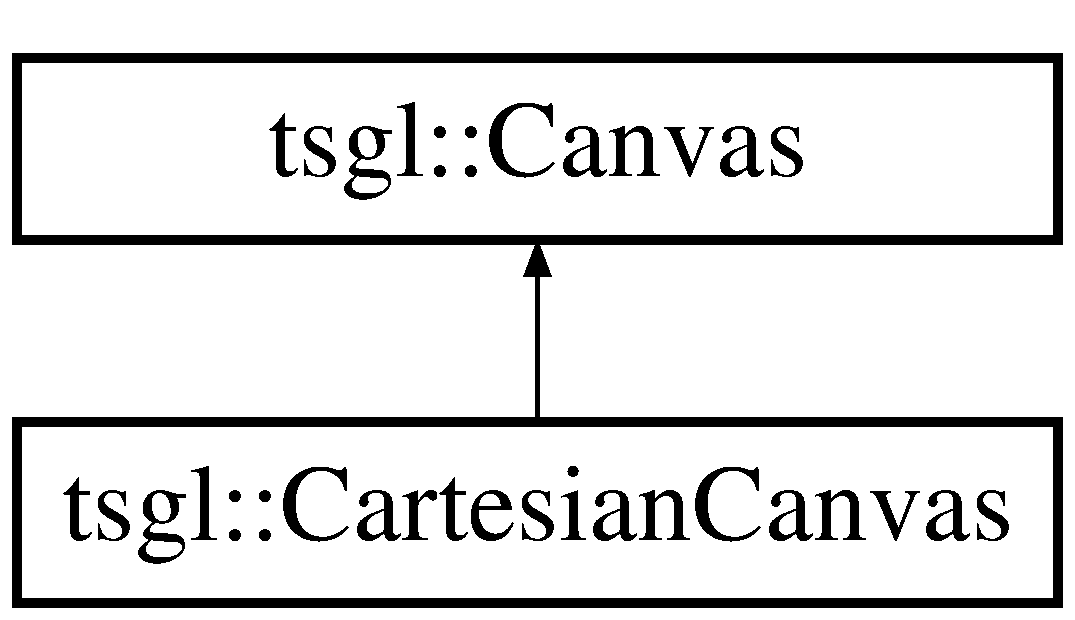
\includegraphics[height=2.000000cm]{classtsgl_1_1_canvas}
\end{center}
\end{figure}
\subsection*{Public Member Functions}
\begin{DoxyCompactItemize}
\item 
\hyperlink{classtsgl_1_1_canvas_ac7e73a23238b067d0b91f73f3af53623}{Canvas} (double timer\+Length=0.\+0f)
\begin{DoxyCompactList}\small\item\em Default \hyperlink{classtsgl_1_1_canvas}{Canvas} constructor method. \end{DoxyCompactList}\item 
\hyperlink{classtsgl_1_1_canvas_a6fac624c804bf5a7169507607d5d876d}{Canvas} (int x, int y, int width, int height, std\+::string title, double timer\+Length=0.\+0f)
\begin{DoxyCompactList}\small\item\em Explicit \hyperlink{classtsgl_1_1_canvas}{Canvas} constructor method. \end{DoxyCompactList}\item 
virtual \hyperlink{classtsgl_1_1_canvas_ab976c3999c68347818d64010b641e14f}{$\sim$\+Canvas} ()
\begin{DoxyCompactList}\small\item\em \hyperlink{classtsgl_1_1_canvas}{Canvas} destructor method. \end{DoxyCompactList}\item 
void \hyperlink{classtsgl_1_1_canvas_a26f2f1acf2b80eee95e42bc13dbc7600}{bind\+To\+Button} (Key button, Action action, void\+Function function)
\begin{DoxyCompactList}\small\item\em Binds a key or button to a function. \end{DoxyCompactList}\item 
void \hyperlink{classtsgl_1_1_canvas_aecd3d94790d2e660db380a5e951ae394}{bind\+To\+Scroll} (std\+::function$<$ void(double, double)$>$ function)
\begin{DoxyCompactList}\small\item\em Binds the mouse wheel to a function. \end{DoxyCompactList}\item 
void \hyperlink{classtsgl_1_1_canvas_abe209d60de2c9b2259ab0588c4e30cef}{clear} ()
\begin{DoxyCompactList}\small\item\em Clears the \hyperlink{classtsgl_1_1_canvas}{Canvas}. \end{DoxyCompactList}\item 
void \hyperlink{classtsgl_1_1_canvas_afaa1250b1da6b48b9c170a0655191938}{close} ()
\begin{DoxyCompactList}\small\item\em Closes the \hyperlink{classtsgl_1_1_canvas}{Canvas} window. \end{DoxyCompactList}\item 
virtual void \hyperlink{classtsgl_1_1_canvas_a2162c16f6aeaee01f8e29696f5818c03}{draw\+Circle} (int x, int y, int radius, int sides, \hyperlink{structtsgl_1_1_color_float}{Color\+Float} color=B\+L\+A\+C\+K, bool filled=true)
\begin{DoxyCompactList}\small\item\em Draws a circle. \end{DoxyCompactList}\item 
virtual void \hyperlink{classtsgl_1_1_canvas_a2165615afc3cebfe38e4313c25bd17b9}{draw\+Colored\+Polygon} (int size, int xverts\mbox{[}$\,$\mbox{]}, int yverts\mbox{[}$\,$\mbox{]}, \hyperlink{structtsgl_1_1_color_float}{Color\+Float} color\mbox{[}$\,$\mbox{]}, bool filled=true)
\begin{DoxyCompactList}\small\item\em Draws an arbitrary polygon with colored vertices. \end{DoxyCompactList}\item 
virtual void \hyperlink{classtsgl_1_1_canvas_ad98cb8db661ef24279b61c4c11fd29ea}{draw\+Concave\+Polygon} (int size, int xverts\mbox{[}$\,$\mbox{]}, int yverts\mbox{[}$\,$\mbox{]}, \hyperlink{structtsgl_1_1_color_float}{Color\+Float} color\mbox{[}$\,$\mbox{]}, bool filled=true)
\begin{DoxyCompactList}\small\item\em Draws a concave polygon with colored vertices. \end{DoxyCompactList}\item 
virtual void \hyperlink{classtsgl_1_1_canvas_a9cb84248c3559c81e4cb2e0d194b2437}{draw\+Convex\+Polygon} (int size, int xverts\mbox{[}$\,$\mbox{]}, int yverts\mbox{[}$\,$\mbox{]}, \hyperlink{structtsgl_1_1_color_float}{Color\+Float} color\mbox{[}$\,$\mbox{]}, bool filled=true)
\begin{DoxyCompactList}\small\item\em Draws a convex polygon with colored vertices. \end{DoxyCompactList}\item 
virtual void \hyperlink{classtsgl_1_1_canvas_ae94a586629d20b7fabcb402d1c654628}{draw\+Image} (std\+::string filename, int x, int y, int width, int height, float alpha=1.\+0f)
\begin{DoxyCompactList}\small\item\em Draws an image. \end{DoxyCompactList}\item 
virtual void \hyperlink{classtsgl_1_1_canvas_a6e5c605b03a69e615fe4ccee30be1959}{draw\+Line} (int x1, int y1, int x2, int y2, \hyperlink{structtsgl_1_1_color_float}{Color\+Float} color=B\+L\+A\+C\+K)
\begin{DoxyCompactList}\small\item\em Draws a line. \end{DoxyCompactList}\item 
virtual void \hyperlink{classtsgl_1_1_canvas_af17d456eca4ad5a55842f2cf02f48a97}{draw\+Pixel} (int row, int col, \hyperlink{structtsgl_1_1_color_float}{Color\+Float} color=B\+L\+A\+C\+K)
\begin{DoxyCompactList}\small\item\em Draws a single pixel, specified in row,column format. \end{DoxyCompactList}\item 
virtual void \hyperlink{classtsgl_1_1_canvas_a6c17c90cd13f7b0184a25e4acc2b7426}{draw\+Point} (int x, int y, \hyperlink{structtsgl_1_1_color_float}{Color\+Float} color=B\+L\+A\+C\+K)
\begin{DoxyCompactList}\small\item\em Draws a single pixel, specified in x,y format. \end{DoxyCompactList}\item 
virtual void \hyperlink{classtsgl_1_1_canvas_aea792059486ebe6d25d7f81bdadf751d}{draw\+Progress} (\hyperlink{classtsgl_1_1_progress_bar}{Progress\+Bar} $\ast$p)
\begin{DoxyCompactList}\small\item\em Draws a progress bar. \end{DoxyCompactList}\item 
virtual void \hyperlink{classtsgl_1_1_canvas_a752754cd16d14447cb5e5b0438bebf16}{draw\+Rectangle} (int x1, int y1, int x2, int y2, \hyperlink{structtsgl_1_1_color_float}{Color\+Float} color=B\+L\+A\+C\+K, bool filled=true)
\begin{DoxyCompactList}\small\item\em Draws a rectangle. \end{DoxyCompactList}\item 
virtual void \hyperlink{classtsgl_1_1_canvas_a3457e7ebd17fa5003025ff6bcaaeedf6}{draw\+Text} (std\+::string text, int x, int y, unsigned size, \hyperlink{structtsgl_1_1_color_float}{Color\+Float} color=B\+L\+A\+C\+K)
\begin{DoxyCompactList}\small\item\em Draw a string of text. \end{DoxyCompactList}\item 
virtual void \hyperlink{classtsgl_1_1_canvas_a1873adb0f3f43e3ebec33fdaf6c6a3d5}{draw\+Text} (std\+::wstring text, int x, int y, unsigned int size, \hyperlink{structtsgl_1_1_color_float}{Color\+Float} color)
\begin{DoxyCompactList}\small\item\em Draws a string of text. \end{DoxyCompactList}\item 
virtual void \hyperlink{classtsgl_1_1_canvas_a8abc9ed7d3c55c5d701009040c65000e}{draw\+Triangle} (int x1, int y1, int x2, int y2, int x3, int y3, \hyperlink{structtsgl_1_1_color_float}{Color\+Float} color=B\+L\+A\+C\+K, bool filled=true)
\begin{DoxyCompactList}\small\item\em Draws a triangle. \end{DoxyCompactList}\item 
\hyperlink{structtsgl_1_1_color_float}{Color\+Float} \hyperlink{classtsgl_1_1_canvas_a2b39e50888d61e88527a66ac0f6ac880}{get\+Background\+Color} ()
\begin{DoxyCompactList}\small\item\em Accessor for the current background color. \end{DoxyCompactList}\item 
int \hyperlink{classtsgl_1_1_canvas_af4f8f2b1abd27316a4a39ae097407d37}{get\+Frame\+Number} ()
\begin{DoxyCompactList}\small\item\em Accessor for the current frame number. \end{DoxyCompactList}\item 
float \hyperlink{classtsgl_1_1_canvas_a1c8ac321138948650a3006f325dfb886}{get\+F\+P\+S} ()
\begin{DoxyCompactList}\small\item\em Accessor for the current F\+P\+S. \end{DoxyCompactList}\item 
bool \hyperlink{classtsgl_1_1_canvas_aa933363de2d19ec516603a2ed3b4f817}{get\+Is\+Open} ()
\begin{DoxyCompactList}\small\item\em Accessor for window\textquotesingle{}s closed status. \end{DoxyCompactList}\item 
int \hyperlink{classtsgl_1_1_canvas_a4af9bed83746f998474039185d2a765a}{get\+Mouse\+X} ()
\begin{DoxyCompactList}\small\item\em Accessor for the mouse\textquotesingle{}s x-\/position. \end{DoxyCompactList}\item 
int \hyperlink{classtsgl_1_1_canvas_a7fc8592848aaa14c3ff440d0ed3c9e4f}{get\+Mouse\+Y} ()
\begin{DoxyCompactList}\small\item\em Accessor for the mouse\textquotesingle{}s y-\/position. \end{DoxyCompactList}\item 
\hyperlink{structtsgl_1_1_color_int}{Color\+Int} \hyperlink{classtsgl_1_1_canvas_a1f54dba4b09d248e2611f3409353c2c6}{get\+Pixel} (int row, int col)
\begin{DoxyCompactList}\small\item\em Gets the color of the pixel drawn on the current \hyperlink{classtsgl_1_1_canvas}{Canvas} at the given screen coordinates, specified in row,column format. \end{DoxyCompactList}\item 
\hyperlink{structtsgl_1_1_color_int}{Color\+Int} \hyperlink{classtsgl_1_1_canvas_aa31883b3c9b09006cf82b270ad7a0a9f}{get\+Point} (int x, int y)
\begin{DoxyCompactList}\small\item\em Gets the color of the pixel drawn on the current \hyperlink{classtsgl_1_1_canvas}{Canvas} at the given screen coordinates, specified in x,y format. \end{DoxyCompactList}\item 
unsigned int \hyperlink{classtsgl_1_1_canvas_a8f0819f368b41b147f1a7f560a7af6a4}{get\+Reps} () const 
\begin{DoxyCompactList}\small\item\em Accessor for the number of theoretical draw cycles that have elapsed. \end{DoxyCompactList}\item 
uint8\+\_\+t $\ast$ \hyperlink{classtsgl_1_1_canvas_a71f072dd82ca3b5cecfd65cde6d8a226}{get\+Screen\+Buffer} ()
\begin{DoxyCompactList}\small\item\em Accessor for the \hyperlink{classtsgl_1_1_canvas}{Canvas}\textquotesingle{}s currently drawn image. \end{DoxyCompactList}\item 
double \hyperlink{classtsgl_1_1_canvas_aef462ab48e59571b9c88076bbdc8f0b3}{get\+Time} ()
\begin{DoxyCompactList}\small\item\em Accessor for the time since the \hyperlink{classtsgl_1_1_canvas}{Canvas} was initialized. \end{DoxyCompactList}\item 
double \hyperlink{classtsgl_1_1_canvas_a8786d28042b767f5c075361100227af4}{get\+Time\+Between\+Sleeps} () const 
\begin{DoxyCompactList}\small\item\em Accessor that gets the time between two sleep times of the internal drawing timer of a \hyperlink{classtsgl_1_1_canvas}{Canvas} object. \end{DoxyCompactList}\item 
int \hyperlink{classtsgl_1_1_canvas_ad740ebe5d6bd69ab79cde3e84f369f35}{get\+Window\+Height} ()
\begin{DoxyCompactList}\small\item\em Accessor for the \hyperlink{classtsgl_1_1_canvas}{Canvas}\textquotesingle{}s window height. \end{DoxyCompactList}\item 
int \hyperlink{classtsgl_1_1_canvas_a086a0322f4a6ab27da6929b1aa0593af}{get\+Window\+Width} ()
\begin{DoxyCompactList}\small\item\em Accessor for the \hyperlink{classtsgl_1_1_canvas}{Canvas}\textquotesingle{}s window width. \end{DoxyCompactList}\item 
int \hyperlink{classtsgl_1_1_canvas_a011ce2354d4565f9d2a323411a47d52d}{get\+Window\+X} ()
\begin{DoxyCompactList}\small\item\em Accessor for the \hyperlink{classtsgl_1_1_canvas}{Canvas}\textquotesingle{}s x-\/position. \end{DoxyCompactList}\item 
int \hyperlink{classtsgl_1_1_canvas_ad6e98d17d3e43d79628a3bd05221ee8b}{get\+Window\+Y} ()
\begin{DoxyCompactList}\small\item\em Accessor for the \hyperlink{classtsgl_1_1_canvas}{Canvas}\textquotesingle{}s y-\/position. \end{DoxyCompactList}\item 
void \hyperlink{classtsgl_1_1_canvas_aa499851e5e4b97bb99ca4fb3d633c17e}{handle\+I\+O} ()
\begin{DoxyCompactList}\small\item\em Manually handles keyboard/mouse I/\+O. \end{DoxyCompactList}\item 
void \hyperlink{classtsgl_1_1_canvas_abe021ab5148cc1327523689bced0f35a}{pause\+Drawing} ()
\begin{DoxyCompactList}\small\item\em Pauses the rendering thread of the \hyperlink{classtsgl_1_1_canvas}{Canvas}. \end{DoxyCompactList}\item 
void \hyperlink{classtsgl_1_1_canvas_a47436daa39473ddb4044bac7b3b27151}{record\+For\+Num\+Frames} (unsigned int num\+\_\+frames)
\begin{DoxyCompactList}\small\item\em Records the \hyperlink{classtsgl_1_1_canvas}{Canvas} for a specified number of frames. \end{DoxyCompactList}\item 
\hypertarget{classtsgl_1_1_canvas_ada6403439b583910d27e497148da5f2e}{}void \hyperlink{classtsgl_1_1_canvas_ada6403439b583910d27e497148da5f2e}{reset} ()\label{classtsgl_1_1_canvas_ada6403439b583910d27e497148da5f2e}

\begin{DoxyCompactList}\small\item\em Resets the internal drawing timer of a \hyperlink{classtsgl_1_1_canvas}{Canvas} instance. \end{DoxyCompactList}\item 
void \hyperlink{classtsgl_1_1_canvas_a56bf3c6e4eb7b06015d1c115aaa143f8}{resume\+Drawing} ()
\begin{DoxyCompactList}\small\item\em Resumes the rendering thread of the \hyperlink{classtsgl_1_1_canvas}{Canvas}. \end{DoxyCompactList}\item 
void \hyperlink{classtsgl_1_1_canvas_abb668fe42e2fe7f269b255152df959d8}{set\+Background\+Color} (\hyperlink{structtsgl_1_1_color_float}{Color\+Float} color)
\begin{DoxyCompactList}\small\item\em Mutator for the background color. \end{DoxyCompactList}\item 
void \hyperlink{classtsgl_1_1_canvas_a692edf8e37c7714cdf2a58ea530c63e9}{set\+Font} (std\+::string filename)
\begin{DoxyCompactList}\small\item\em Mutator for the currently loaded font. \end{DoxyCompactList}\item 
void \hyperlink{classtsgl_1_1_canvas_a8722c579dfa55a45e139bfeb269d73ff}{set\+Show\+F\+P\+S} (bool b)
\begin{DoxyCompactList}\small\item\em Mutator for showing the F\+P\+S. \end{DoxyCompactList}\item 
void \hyperlink{classtsgl_1_1_canvas_a2604fa056d4541f918ccf447eda1f3cf}{sleep} ()
\begin{DoxyCompactList}\small\item\em Sleeps the calling thread to sync with the \hyperlink{classtsgl_1_1_canvas}{Canvas}. \end{DoxyCompactList}\item 
void \hyperlink{classtsgl_1_1_canvas_a6674cc86b9a54b6a564021fddce47e36}{sleep\+For} (float seconds)
\begin{DoxyCompactList}\small\item\em Sleeps the calling thread for a set amount of time. \end{DoxyCompactList}\item 
int \hyperlink{classtsgl_1_1_canvas_a654315f9b08a9b3b072eebf4b4d8ae89}{start} ()
\begin{DoxyCompactList}\small\item\em Opens the \hyperlink{classtsgl_1_1_canvas}{Canvas}. \end{DoxyCompactList}\item 
void \hyperlink{classtsgl_1_1_canvas_a46cd37a9f2a146e57b4e0273faf6485c}{stop} ()
\begin{DoxyCompactList}\small\item\em Begins the process of closing the \hyperlink{classtsgl_1_1_canvas}{Canvas}. \end{DoxyCompactList}\item 
void \hyperlink{classtsgl_1_1_canvas_ac6035d87aa3bf077031bc0bb6f419b17}{stop\+Recording} ()
\begin{DoxyCompactList}\small\item\em Stops recording the \hyperlink{classtsgl_1_1_canvas}{Canvas}. \end{DoxyCompactList}\item 
void \hyperlink{classtsgl_1_1_canvas_ac035f43763b198f6915a0772973a5ea9}{take\+Screen\+Shot} ()
\begin{DoxyCompactList}\small\item\em Takes a screenshot. \end{DoxyCompactList}\item 
int \hyperlink{classtsgl_1_1_canvas_a39e69fd4d1ad8cf0e22ecea12f1ddf08}{wait} ()
\begin{DoxyCompactList}\small\item\em Waits for the user to close the \hyperlink{classtsgl_1_1_canvas}{Canvas}. \end{DoxyCompactList}\end{DoxyCompactItemize}
\subsection*{Static Public Member Functions}
\begin{DoxyCompactItemize}
\item 
static int \hyperlink{classtsgl_1_1_canvas_a664b101f972845eaf5fdc4d9e664e623}{get\+Display\+Height} ()
\begin{DoxyCompactList}\small\item\em Accessor for the height of the user\textquotesingle{}s primary monitor. \end{DoxyCompactList}\item 
static int \hyperlink{classtsgl_1_1_canvas_abbe5c392cac2320fecf1f2751afb207c}{get\+Display\+Width} ()
\begin{DoxyCompactList}\small\item\em Accessor for the width of the user\textquotesingle{}s primary monitor. \end{DoxyCompactList}\item 
\hypertarget{classtsgl_1_1_canvas_a3365d92635f650cca2eda69812bef60b}{}static void \hyperlink{classtsgl_1_1_canvas_a3365d92635f650cca2eda69812bef60b}{run\+Tests} ()\label{classtsgl_1_1_canvas_a3365d92635f650cca2eda69812bef60b}

\begin{DoxyCompactList}\small\item\em Runs unit tests for the \hyperlink{classtsgl_1_1_canvas}{Canvas}. \end{DoxyCompactList}\end{DoxyCompactItemize}
\subsection*{Protected Member Functions}
\begin{DoxyCompactItemize}
\item 
\hypertarget{classtsgl_1_1_canvas_a560e3f64f3b2e5a7af8a8d7b92d8e660}{}void {\bfseries draw\+Shape} (\hyperlink{classtsgl_1_1_shape}{Shape} $\ast$s)\label{classtsgl_1_1_canvas_a560e3f64f3b2e5a7af8a8d7b92d8e660}

\end{DoxyCompactItemize}
\subsection*{Protected Attributes}
\begin{DoxyCompactItemize}
\item 
\hypertarget{classtsgl_1_1_canvas_a1558f2f09228ccaf0d46cec233a2dac7}{}bool {\bfseries ati\+Card}\label{classtsgl_1_1_canvas_a1558f2f09228ccaf0d46cec233a2dac7}

\end{DoxyCompactItemize}


\subsection{Detailed Description}
A G\+L window with numerous built-\/in, thread-\/safe drawing operations. 

\hyperlink{classtsgl_1_1_canvas}{Canvas} provides an easy-\/to-\/set-\/up, easy-\/to-\/use class for drawing various shapes.

Using stb, \hyperlink{classtsgl_1_1_canvas}{Canvas} also supports the drawing of images.

On top of being easy to use, \hyperlink{classtsgl_1_1_canvas}{Canvas} is also thread-\/safe, so any number of images may be drawn at once. \begin{DoxyNote}{Note}
{\bfseries O\+S X\+:} Due to the way O\+S X handles I/\+O, either \hyperlink{classtsgl_1_1_canvas_a2604fa056d4541f918ccf447eda1f3cf}{sleep()} or \hyperlink{classtsgl_1_1_canvas_aa499851e5e4b97bb99ca4fb3d633c17e}{handle\+I\+O()} must be manually called whenever the user wants to handle any input/output events (keyboard/mouse presses). Whenever a window is created using Open\+G\+L, O\+S X requires the main thread to handle I/\+O calls. 

{\bfseries O\+S X\+:} O\+S X also uses p\+\_\+thread instead of std\+::thread for threading. 
\end{DoxyNote}


\subsection{Constructor \& Destructor Documentation}
\hypertarget{classtsgl_1_1_canvas_ac7e73a23238b067d0b91f73f3af53623}{}\index{tsgl\+::\+Canvas@{tsgl\+::\+Canvas}!Canvas@{Canvas}}
\index{Canvas@{Canvas}!tsgl\+::\+Canvas@{tsgl\+::\+Canvas}}
\subsubsection[{Canvas}]{\setlength{\rightskip}{0pt plus 5cm}tsgl\+::\+Canvas\+::\+Canvas (
\begin{DoxyParamCaption}
\item[{double}]{timer\+Length = {\ttfamily 0.0f}}
\end{DoxyParamCaption}
)}\label{classtsgl_1_1_canvas_ac7e73a23238b067d0b91f73f3af53623}


Default \hyperlink{classtsgl_1_1_canvas}{Canvas} constructor method. 

This is the default constructor for the \hyperlink{classtsgl_1_1_canvas}{Canvas} class. 
\begin{DoxyParams}{Parameters}
{\em timer\+Length} & The minimum number of seconds between draw cycles for the \hyperlink{classtsgl_1_1_canvas}{Canvas}. A value less than or equal to 0 sets it to automatic. \\
\hline
\end{DoxyParams}
\begin{DoxyReturn}{Returns}
A new \hyperlink{classtsgl_1_1_canvas}{Canvas} in the middle of the screen with no title. The created \hyperlink{classtsgl_1_1_canvas}{Canvas} will take up approximately 90\% of the monitor\textquotesingle{}s height, and will have a 4\+:3 aspect ratio. 
\end{DoxyReturn}
\hypertarget{classtsgl_1_1_canvas_a6fac624c804bf5a7169507607d5d876d}{}\index{tsgl\+::\+Canvas@{tsgl\+::\+Canvas}!Canvas@{Canvas}}
\index{Canvas@{Canvas}!tsgl\+::\+Canvas@{tsgl\+::\+Canvas}}
\subsubsection[{Canvas}]{\setlength{\rightskip}{0pt plus 5cm}tsgl\+::\+Canvas\+::\+Canvas (
\begin{DoxyParamCaption}
\item[{int}]{x, }
\item[{int}]{y, }
\item[{int}]{width, }
\item[{int}]{height, }
\item[{std\+::string}]{title, }
\item[{double}]{timer\+Length = {\ttfamily 0.0f}}
\end{DoxyParamCaption}
)}\label{classtsgl_1_1_canvas_a6fac624c804bf5a7169507607d5d876d}


Explicit \hyperlink{classtsgl_1_1_canvas}{Canvas} constructor method. 

This is the explicit constructor for the \hyperlink{classtsgl_1_1_canvas}{Canvas} class. 
\begin{DoxyParams}{Parameters}
{\em x} & The x position of the \hyperlink{classtsgl_1_1_canvas}{Canvas} window. \\
\hline
{\em y} & The y position of the \hyperlink{classtsgl_1_1_canvas}{Canvas} window. \\
\hline
{\em width} & The x dimension of the \hyperlink{classtsgl_1_1_canvas}{Canvas} window. \\
\hline
{\em height} & The y dimension of the \hyperlink{classtsgl_1_1_canvas}{Canvas} window. \\
\hline
{\em title} & The title of the window. \\
\hline
{\em timer\+Length} & The minimum number of seconds between draw cycles for the \hyperlink{classtsgl_1_1_canvas}{Canvas}. A value less than or equal to 0 sets it to automatic. \\
\hline
\end{DoxyParams}
\begin{DoxyReturn}{Returns}
A new \hyperlink{classtsgl_1_1_canvas}{Canvas} with the specified position, dimensions, title, and draw cycle length. 
\end{DoxyReturn}
\hypertarget{classtsgl_1_1_canvas_ab976c3999c68347818d64010b641e14f}{}\index{tsgl\+::\+Canvas@{tsgl\+::\+Canvas}!````~Canvas@{$\sim$\+Canvas}}
\index{````~Canvas@{$\sim$\+Canvas}!tsgl\+::\+Canvas@{tsgl\+::\+Canvas}}
\subsubsection[{$\sim$\+Canvas}]{\setlength{\rightskip}{0pt plus 5cm}tsgl\+::\+Canvas\+::$\sim$\+Canvas (
\begin{DoxyParamCaption}
{}
\end{DoxyParamCaption}
)\hspace{0.3cm}{\ttfamily [virtual]}}\label{classtsgl_1_1_canvas_ab976c3999c68347818d64010b641e14f}


\hyperlink{classtsgl_1_1_canvas}{Canvas} destructor method. 

This is the destructor for the \hyperlink{classtsgl_1_1_canvas}{Canvas} class.

Frees up memory that was allocated to a \hyperlink{classtsgl_1_1_canvas}{Canvas} instance. 

\subsection{Member Function Documentation}
\hypertarget{classtsgl_1_1_canvas_a26f2f1acf2b80eee95e42bc13dbc7600}{}\index{tsgl\+::\+Canvas@{tsgl\+::\+Canvas}!bind\+To\+Button@{bind\+To\+Button}}
\index{bind\+To\+Button@{bind\+To\+Button}!tsgl\+::\+Canvas@{tsgl\+::\+Canvas}}
\subsubsection[{bind\+To\+Button}]{\setlength{\rightskip}{0pt plus 5cm}void tsgl\+::\+Canvas\+::bind\+To\+Button (
\begin{DoxyParamCaption}
\item[{Key}]{button, }
\item[{Action}]{action, }
\item[{void\+Function}]{function}
\end{DoxyParamCaption}
)}\label{classtsgl_1_1_canvas_a26f2f1acf2b80eee95e42bc13dbc7600}


Binds a key or button to a function. 

This function binds a key or mouse button to a function pointer.

Upon pressing or releasing the given key, \hyperlink{classtsgl_1_1_canvas}{Canvas} will call the specified function. 
\begin{DoxyParams}{Parameters}
{\em button} & The key or button to bind, as specified in \hyperlink{_keynums_8h_source}{Keynums.\+h}. \\
\hline
{\em action} & The action to look out for (T\+S\+G\+L\+\_\+\+P\+R\+E\+S\+S or T\+S\+G\+L\+\_\+\+R\+E\+L\+E\+A\+S\+E). \\
\hline
{\em function} & The function to call upon action {\ttfamily a} on button. \\
\hline
\end{DoxyParams}
\begin{DoxyWarning}{Warning}
{\bfseries T\+S\+G\+L\+\_\+\+K\+E\+Y\+\_\+\+E\+S\+C\+A\+P\+E is automatically bound to closing the window. Overriding T\+S\+G\+L\+\_\+\+K\+E\+Y\+\_\+\+E\+S\+C\+A\+P\+E will likely make you unable to close the window through the escape key.} 
\end{DoxyWarning}
\hypertarget{classtsgl_1_1_canvas_aecd3d94790d2e660db380a5e951ae394}{}\index{tsgl\+::\+Canvas@{tsgl\+::\+Canvas}!bind\+To\+Scroll@{bind\+To\+Scroll}}
\index{bind\+To\+Scroll@{bind\+To\+Scroll}!tsgl\+::\+Canvas@{tsgl\+::\+Canvas}}
\subsubsection[{bind\+To\+Scroll}]{\setlength{\rightskip}{0pt plus 5cm}void tsgl\+::\+Canvas\+::bind\+To\+Scroll (
\begin{DoxyParamCaption}
\item[{std\+::function$<$ void(double, double)$>$}]{function}
\end{DoxyParamCaption}
)}\label{classtsgl_1_1_canvas_aecd3d94790d2e660db380a5e951ae394}


Binds the mouse wheel to a function. 

This function binds the mouse wheel to a function pointer.

Upon scrolling, \hyperlink{classtsgl_1_1_canvas}{Canvas} will call the specified function. 
\begin{DoxyParams}{Parameters}
{\em function} & A function taking x and y parameters to be called when the mouse is scrolled. \\
\hline
\end{DoxyParams}
\hypertarget{classtsgl_1_1_canvas_abe209d60de2c9b2259ab0588c4e30cef}{}\index{tsgl\+::\+Canvas@{tsgl\+::\+Canvas}!clear@{clear}}
\index{clear@{clear}!tsgl\+::\+Canvas@{tsgl\+::\+Canvas}}
\subsubsection[{clear}]{\setlength{\rightskip}{0pt plus 5cm}void tsgl\+::\+Canvas\+::clear (
\begin{DoxyParamCaption}
{}
\end{DoxyParamCaption}
)}\label{classtsgl_1_1_canvas_abe209d60de2c9b2259ab0588c4e30cef}


Clears the \hyperlink{classtsgl_1_1_canvas}{Canvas}. 

This function clears the screen to the color specified in \hyperlink{classtsgl_1_1_canvas_abb668fe42e2fe7f269b255152df959d8}{set\+Background\+Color()}. 

Referenced by tsgl\+::\+Spectrogram\+::draw().

\hypertarget{classtsgl_1_1_canvas_afaa1250b1da6b48b9c170a0655191938}{}\index{tsgl\+::\+Canvas@{tsgl\+::\+Canvas}!close@{close}}
\index{close@{close}!tsgl\+::\+Canvas@{tsgl\+::\+Canvas}}
\subsubsection[{close}]{\setlength{\rightskip}{0pt plus 5cm}void tsgl\+::\+Canvas\+::close (
\begin{DoxyParamCaption}
{}
\end{DoxyParamCaption}
)}\label{classtsgl_1_1_canvas_afaa1250b1da6b48b9c170a0655191938}


Closes the \hyperlink{classtsgl_1_1_canvas}{Canvas} window. 

This function tells the \hyperlink{classtsgl_1_1_canvas}{Canvas} to stop rendering and to close its rendering window.

Any threads that have called \hyperlink{classtsgl_1_1_canvas_a39e69fd4d1ad8cf0e22ecea12f1ddf08}{wait()} will continue. \begin{DoxySeeAlso}{See also}
\hyperlink{classtsgl_1_1_canvas_a654315f9b08a9b3b072eebf4b4d8ae89}{start()}, \hyperlink{classtsgl_1_1_canvas_a46cd37a9f2a146e57b4e0273faf6485c}{stop()}, \hyperlink{classtsgl_1_1_canvas_a39e69fd4d1ad8cf0e22ecea12f1ddf08}{wait()} 
\end{DoxySeeAlso}


Referenced by tsgl\+::\+Visual\+Task\+Queue\+::close(), and stop().

\hypertarget{classtsgl_1_1_canvas_a2162c16f6aeaee01f8e29696f5818c03}{}\index{tsgl\+::\+Canvas@{tsgl\+::\+Canvas}!draw\+Circle@{draw\+Circle}}
\index{draw\+Circle@{draw\+Circle}!tsgl\+::\+Canvas@{tsgl\+::\+Canvas}}
\subsubsection[{draw\+Circle}]{\setlength{\rightskip}{0pt plus 5cm}void tsgl\+::\+Canvas\+::draw\+Circle (
\begin{DoxyParamCaption}
\item[{int}]{x, }
\item[{int}]{y, }
\item[{int}]{radius, }
\item[{int}]{sides, }
\item[{{\bf Color\+Float}}]{color = {\ttfamily BLACK}, }
\item[{bool}]{filled = {\ttfamily true}}
\end{DoxyParamCaption}
)\hspace{0.3cm}{\ttfamily [virtual]}}\label{classtsgl_1_1_canvas_a2162c16f6aeaee01f8e29696f5818c03}


Draws a circle. 

This function draws a circle with the given center, radius, resolution (number of sides), color, and fill status. 
\begin{DoxyParams}{Parameters}
{\em x} & The x coordinate of the circle\textquotesingle{}s center. \\
\hline
{\em y} & The y coordinate of the circle\textquotesingle{}s center. \\
\hline
{\em radius} & The radius of the circle in pixels. \\
\hline
{\em sides} & The number of sides to use in the circle. \\
\hline
{\em color} & The color of the circle (set to B\+L\+A\+C\+K by default). \\
\hline
{\em filled} & Whether the circle should be filled (set to true by default). \\
\hline
\end{DoxyParams}


Referenced by tsgl\+::\+Cartesian\+Canvas\+::draw\+Circle().

\hypertarget{classtsgl_1_1_canvas_a2165615afc3cebfe38e4313c25bd17b9}{}\index{tsgl\+::\+Canvas@{tsgl\+::\+Canvas}!draw\+Colored\+Polygon@{draw\+Colored\+Polygon}}
\index{draw\+Colored\+Polygon@{draw\+Colored\+Polygon}!tsgl\+::\+Canvas@{tsgl\+::\+Canvas}}
\subsubsection[{draw\+Colored\+Polygon}]{\setlength{\rightskip}{0pt plus 5cm}void tsgl\+::\+Canvas\+::draw\+Colored\+Polygon (
\begin{DoxyParamCaption}
\item[{int}]{size, }
\item[{int}]{xverts\mbox{[}$\,$\mbox{]}, }
\item[{int}]{yverts\mbox{[}$\,$\mbox{]}, }
\item[{{\bf Color\+Float}}]{color\mbox{[}$\,$\mbox{]}, }
\item[{bool}]{filled = {\ttfamily true}}
\end{DoxyParamCaption}
)\hspace{0.3cm}{\ttfamily [virtual]}}\label{classtsgl_1_1_canvas_a2165615afc3cebfe38e4313c25bd17b9}


Draws an arbitrary polygon with colored vertices. 

This function draws a \hyperlink{classtsgl_1_1_colored_polygon}{Colored\+Polygon} with the given vertex data, specified as a triangle strip. 
\begin{DoxyParams}{Parameters}
{\em size} & The number of vertices in the polygon. \\
\hline
{\em xverts} & An array of x positions of the vertices. \\
\hline
{\em yverts} & An array of y positions of the vertices. \\
\hline
{\em color} & An array of colors for the vertices. \\
\hline
{\em filled} & Whether the colored polygon should be filled (true) or not (false) (set to true by default). \\
\hline
\end{DoxyParams}


Referenced by tsgl\+::\+Cartesian\+Canvas\+::draw\+Colored\+Polygon().

\hypertarget{classtsgl_1_1_canvas_ad98cb8db661ef24279b61c4c11fd29ea}{}\index{tsgl\+::\+Canvas@{tsgl\+::\+Canvas}!draw\+Concave\+Polygon@{draw\+Concave\+Polygon}}
\index{draw\+Concave\+Polygon@{draw\+Concave\+Polygon}!tsgl\+::\+Canvas@{tsgl\+::\+Canvas}}
\subsubsection[{draw\+Concave\+Polygon}]{\setlength{\rightskip}{0pt plus 5cm}void tsgl\+::\+Canvas\+::draw\+Concave\+Polygon (
\begin{DoxyParamCaption}
\item[{int}]{size, }
\item[{int}]{xverts\mbox{[}$\,$\mbox{]}, }
\item[{int}]{yverts\mbox{[}$\,$\mbox{]}, }
\item[{{\bf Color\+Float}}]{color\mbox{[}$\,$\mbox{]}, }
\item[{bool}]{filled = {\ttfamily true}}
\end{DoxyParamCaption}
)\hspace{0.3cm}{\ttfamily [virtual]}}\label{classtsgl_1_1_canvas_ad98cb8db661ef24279b61c4c11fd29ea}


Draws a concave polygon with colored vertices. 

This function draws a \hyperlink{classtsgl_1_1_concave_polygon}{Concave\+Polygon} with the given vertex data, specified as the outer perimeter of the polygon. 
\begin{DoxyParams}{Parameters}
{\em size} & The number of vertices in the polygon. \\
\hline
{\em xverts} & An array of x positions of said vertices. \\
\hline
{\em yverts} & An array of y positions of said vertices. \\
\hline
{\em color} & An array of colors for the said vertices. \\
\hline
{\em filled} & Whether the Concave polygon should be filled in or not (set to true by default). \\
\hline
\end{DoxyParams}
\begin{DoxyWarning}{Warning}
{\bfseries This function is significantly slower than \hyperlink{classtsgl_1_1_canvas_a9cb84248c3559c81e4cb2e0d194b2437}{draw\+Convex\+Polygon()}. It is not recommended that you draw convex polygons with this function. }
\end{DoxyWarning}
\begin{DoxySeeAlso}{See also}
{\bfseries  \hyperlink{classtsgl_1_1_canvas_a9cb84248c3559c81e4cb2e0d194b2437}{draw\+Convex\+Polygon()}. }
\end{DoxySeeAlso}


Referenced by tsgl\+::\+Cartesian\+Canvas\+::draw\+Concave\+Polygon().

\hypertarget{classtsgl_1_1_canvas_a9cb84248c3559c81e4cb2e0d194b2437}{}\index{tsgl\+::\+Canvas@{tsgl\+::\+Canvas}!draw\+Convex\+Polygon@{draw\+Convex\+Polygon}}
\index{draw\+Convex\+Polygon@{draw\+Convex\+Polygon}!tsgl\+::\+Canvas@{tsgl\+::\+Canvas}}
\subsubsection[{draw\+Convex\+Polygon}]{\setlength{\rightskip}{0pt plus 5cm}void tsgl\+::\+Canvas\+::draw\+Convex\+Polygon (
\begin{DoxyParamCaption}
\item[{int}]{size, }
\item[{int}]{xverts\mbox{[}$\,$\mbox{]}, }
\item[{int}]{yverts\mbox{[}$\,$\mbox{]}, }
\item[{{\bf Color\+Float}}]{color\mbox{[}$\,$\mbox{]}, }
\item[{bool}]{filled = {\ttfamily true}}
\end{DoxyParamCaption}
)\hspace{0.3cm}{\ttfamily [virtual]}}\label{classtsgl_1_1_canvas_a9cb84248c3559c81e4cb2e0d194b2437}


Draws a convex polygon with colored vertices. 

This function draws a \hyperlink{classtsgl_1_1_convex_polygon}{Convex\+Polygon} with the given vertex data, specified as the outer perimeter of the polygon. 
\begin{DoxyParams}{Parameters}
{\em size} & The number of vertices in the polygon. \\
\hline
{\em xverts} & An array of the x positions of said vertices. \\
\hline
{\em yverts} & An array of the y positions of said vertices. \\
\hline
{\em color} & An array of colors for the said vertices. \\
\hline
{\em filled} & Whether the \hyperlink{classtsgl_1_1_convex_polygon}{Convex\+Polygon} should be filled in or not (set to true by default). \\
\hline
\end{DoxyParams}
\begin{DoxyNote}{Note}
The difference between a convex polygon and a concave polygon is that a convex polygon has all interior angles less than 180 degrees ( see \href{http://www.mathopenref.com/polygonconvex.html}{\tt http\+://www.\+mathopenref.\+com/polygonconvex.\+html} ). 
\end{DoxyNote}


Referenced by tsgl\+::\+Spectrogram\+::draw(), and tsgl\+::\+Cartesian\+Canvas\+::draw\+Convex\+Polygon().

\hypertarget{classtsgl_1_1_canvas_ae94a586629d20b7fabcb402d1c654628}{}\index{tsgl\+::\+Canvas@{tsgl\+::\+Canvas}!draw\+Image@{draw\+Image}}
\index{draw\+Image@{draw\+Image}!tsgl\+::\+Canvas@{tsgl\+::\+Canvas}}
\subsubsection[{draw\+Image}]{\setlength{\rightskip}{0pt plus 5cm}void tsgl\+::\+Canvas\+::draw\+Image (
\begin{DoxyParamCaption}
\item[{std\+::string}]{filename, }
\item[{int}]{x, }
\item[{int}]{y, }
\item[{int}]{width, }
\item[{int}]{height, }
\item[{float}]{alpha = {\ttfamily 1.0f}}
\end{DoxyParamCaption}
)\hspace{0.3cm}{\ttfamily [virtual]}}\label{classtsgl_1_1_canvas_ae94a586629d20b7fabcb402d1c654628}


Draws an image. 

This function draws an \hyperlink{classtsgl_1_1_image}{Image} with the given coordinates and dimensions. 
\begin{DoxyParams}{Parameters}
{\em filename} & The name of the file to load the image from. \\
\hline
{\em x} & The x coordinate of the \hyperlink{classtsgl_1_1_image}{Image}\textquotesingle{}s left edge. \\
\hline
{\em y} & The y coordinate of the \hyperlink{classtsgl_1_1_image}{Image}\textquotesingle{}s top edge. \\
\hline
{\em width} & The width of the \hyperlink{classtsgl_1_1_image}{Image}. \\
\hline
{\em height} & The height of the \hyperlink{classtsgl_1_1_image}{Image}. \\
\hline
{\em alpha} & The alpha with which to draw the \hyperlink{classtsgl_1_1_image}{Image} \\
\hline
\end{DoxyParams}


Referenced by tsgl\+::\+Cartesian\+Canvas\+::draw\+Image().

\hypertarget{classtsgl_1_1_canvas_a6e5c605b03a69e615fe4ccee30be1959}{}\index{tsgl\+::\+Canvas@{tsgl\+::\+Canvas}!draw\+Line@{draw\+Line}}
\index{draw\+Line@{draw\+Line}!tsgl\+::\+Canvas@{tsgl\+::\+Canvas}}
\subsubsection[{draw\+Line}]{\setlength{\rightskip}{0pt plus 5cm}void tsgl\+::\+Canvas\+::draw\+Line (
\begin{DoxyParamCaption}
\item[{int}]{x1, }
\item[{int}]{y1, }
\item[{int}]{x2, }
\item[{int}]{y2, }
\item[{{\bf Color\+Float}}]{color = {\ttfamily BLACK}}
\end{DoxyParamCaption}
)\hspace{0.3cm}{\ttfamily [virtual]}}\label{classtsgl_1_1_canvas_a6e5c605b03a69e615fe4ccee30be1959}


Draws a line. 

This function draws a \hyperlink{classtsgl_1_1_line}{Line} at the given coordinates with the given color. 
\begin{DoxyParams}{Parameters}
{\em x1} & The x position of the start of the line. \\
\hline
{\em y1} & The y position of the start of the line. \\
\hline
{\em x2} & The x position of the end of the line. \\
\hline
{\em y2} & The y position of the end of the line. \\
\hline
{\em color} & The color of the line (set to B\+L\+A\+C\+K by default). \\
\hline
\end{DoxyParams}


Referenced by tsgl\+::\+Spectrogram\+::draw(), and tsgl\+::\+Cartesian\+Canvas\+::draw\+Line().

\hypertarget{classtsgl_1_1_canvas_af17d456eca4ad5a55842f2cf02f48a97}{}\index{tsgl\+::\+Canvas@{tsgl\+::\+Canvas}!draw\+Pixel@{draw\+Pixel}}
\index{draw\+Pixel@{draw\+Pixel}!tsgl\+::\+Canvas@{tsgl\+::\+Canvas}}
\subsubsection[{draw\+Pixel}]{\setlength{\rightskip}{0pt plus 5cm}void tsgl\+::\+Canvas\+::draw\+Pixel (
\begin{DoxyParamCaption}
\item[{int}]{row, }
\item[{int}]{col, }
\item[{{\bf Color\+Float}}]{color = {\ttfamily BLACK}}
\end{DoxyParamCaption}
)\hspace{0.3cm}{\ttfamily [inline]}, {\ttfamily [virtual]}}\label{classtsgl_1_1_canvas_af17d456eca4ad5a55842f2cf02f48a97}


Draws a single pixel, specified in row,column format. 

This function draws a pixel at the given screen coordinates with the given color. \begin{DoxyNote}{Note}
(0,0) signifies the {\bfseries top-\/left} of the screen when working with a \hyperlink{classtsgl_1_1_canvas}{Canvas} object. 

(0,0) signifies the {\bfseries bottom-\/left} of the screen when working with a \hyperlink{classtsgl_1_1_cartesian_canvas}{Cartesian\+Canvas} object. 
\end{DoxyNote}

\begin{DoxyParams}{Parameters}
{\em row} & The row (y-\/position) of the pixel. \\
\hline
{\em col} & The column (x-\/position) of the pixel. \\
\hline
{\em color} & The color of the point (set to B\+L\+A\+C\+K by default). \\
\hline
\end{DoxyParams}
\begin{DoxySeeAlso}{See also}
\hyperlink{classtsgl_1_1_canvas_a6c17c90cd13f7b0184a25e4acc2b7426}{draw\+Point()} 
\end{DoxySeeAlso}
\hypertarget{classtsgl_1_1_canvas_a6c17c90cd13f7b0184a25e4acc2b7426}{}\index{tsgl\+::\+Canvas@{tsgl\+::\+Canvas}!draw\+Point@{draw\+Point}}
\index{draw\+Point@{draw\+Point}!tsgl\+::\+Canvas@{tsgl\+::\+Canvas}}
\subsubsection[{draw\+Point}]{\setlength{\rightskip}{0pt plus 5cm}void tsgl\+::\+Canvas\+::draw\+Point (
\begin{DoxyParamCaption}
\item[{int}]{x, }
\item[{int}]{y, }
\item[{{\bf Color\+Float}}]{color = {\ttfamily BLACK}}
\end{DoxyParamCaption}
)\hspace{0.3cm}{\ttfamily [virtual]}}\label{classtsgl_1_1_canvas_a6c17c90cd13f7b0184a25e4acc2b7426}


Draws a single pixel, specified in x,y format. 

This function draws a pixel at the given Cartesian coordinates with the given color. \begin{DoxyNote}{Note}
(0,0) signifies the {\bfseries left-\/top} of the screen when working with a \hyperlink{classtsgl_1_1_canvas}{Canvas} object. 

(0,0) signifies the {\bfseries left-\/bottom} of the screen when working with a \hyperlink{classtsgl_1_1_cartesian_canvas}{Cartesian\+Canvas} object. 
\end{DoxyNote}

\begin{DoxyParams}{Parameters}
{\em x} & The x position of the point. \\
\hline
{\em y} & The y position of the point. \\
\hline
{\em color} & The color of the point (set to B\+L\+A\+C\+K by default). \\
\hline
\end{DoxyParams}
\begin{DoxySeeAlso}{See also}
\hyperlink{classtsgl_1_1_canvas_af17d456eca4ad5a55842f2cf02f48a97}{draw\+Pixel()} 
\end{DoxySeeAlso}


Referenced by draw\+Pixel(), and tsgl\+::\+Cartesian\+Canvas\+::draw\+Point().

\hypertarget{classtsgl_1_1_canvas_aea792059486ebe6d25d7f81bdadf751d}{}\index{tsgl\+::\+Canvas@{tsgl\+::\+Canvas}!draw\+Progress@{draw\+Progress}}
\index{draw\+Progress@{draw\+Progress}!tsgl\+::\+Canvas@{tsgl\+::\+Canvas}}
\subsubsection[{draw\+Progress}]{\setlength{\rightskip}{0pt plus 5cm}void tsgl\+::\+Canvas\+::draw\+Progress (
\begin{DoxyParamCaption}
\item[{{\bf Progress\+Bar} $\ast$}]{p}
\end{DoxyParamCaption}
)\hspace{0.3cm}{\ttfamily [virtual]}}\label{classtsgl_1_1_canvas_aea792059486ebe6d25d7f81bdadf751d}


Draws a progress bar. 

This function draws a previously created \hyperlink{classtsgl_1_1_progress_bar}{Progress\+Bar} to the \hyperlink{classtsgl_1_1_canvas}{Canvas}, as specified in that \hyperlink{classtsgl_1_1_progress_bar}{Progress\+Bar}\textquotesingle{}s constructor. 
\begin{DoxyParams}{Parameters}
{\em p} & A pointer to a \hyperlink{classtsgl_1_1_progress_bar}{Progress\+Bar}. \\
\hline
\end{DoxyParams}
\begin{DoxyNote}{Note}
There is no equivalent function for \hyperlink{classtsgl_1_1_cartesian_canvas}{Cartesian\+Canvas}. If you\textquotesingle{}d like to draw a \hyperlink{classtsgl_1_1_progress_bar}{Progress\+Bar} on a \hyperlink{classtsgl_1_1_cartesian_canvas}{Cartesian\+Canvas}, you can still use this function, but you must use absolute \hyperlink{classtsgl_1_1_canvas}{Canvas} coordinates rather than the scaled \hyperlink{classtsgl_1_1_cartesian_canvas}{Cartesian\+Canvas} coordinates. 
\end{DoxyNote}
\hypertarget{classtsgl_1_1_canvas_a752754cd16d14447cb5e5b0438bebf16}{}\index{tsgl\+::\+Canvas@{tsgl\+::\+Canvas}!draw\+Rectangle@{draw\+Rectangle}}
\index{draw\+Rectangle@{draw\+Rectangle}!tsgl\+::\+Canvas@{tsgl\+::\+Canvas}}
\subsubsection[{draw\+Rectangle}]{\setlength{\rightskip}{0pt plus 5cm}void tsgl\+::\+Canvas\+::draw\+Rectangle (
\begin{DoxyParamCaption}
\item[{int}]{x1, }
\item[{int}]{y1, }
\item[{int}]{x2, }
\item[{int}]{y2, }
\item[{{\bf Color\+Float}}]{color = {\ttfamily BLACK}, }
\item[{bool}]{filled = {\ttfamily true}}
\end{DoxyParamCaption}
)\hspace{0.3cm}{\ttfamily [virtual]}}\label{classtsgl_1_1_canvas_a752754cd16d14447cb5e5b0438bebf16}


Draws a rectangle. 

This function draws a \hyperlink{classtsgl_1_1_rectangle}{Rectangle} with the given coordinates, dimensions, and color. 
\begin{DoxyParams}{Parameters}
{\em x1} & The x coordinate of the \hyperlink{classtsgl_1_1_rectangle}{Rectangle}\textquotesingle{}s left edge. \\
\hline
{\em y1} & The y coordinate of the \hyperlink{classtsgl_1_1_rectangle}{Rectangle}\textquotesingle{}s top edge. \\
\hline
{\em x2} & The x coordinate of the \hyperlink{classtsgl_1_1_rectangle}{Rectangle}\textquotesingle{}s right edge. \\
\hline
{\em y2} & The y coordinate of the \hyperlink{classtsgl_1_1_rectangle}{Rectangle}\textquotesingle{}s bottom edge. \\
\hline
{\em color} & The color of the rectangle (set to B\+L\+A\+C\+K by default). \\
\hline
{\em filled} & Whether the rectangle should be filled (set to true by default). \\
\hline
\end{DoxyParams}
\begin{DoxyRefDesc}{Bug}
\item[\hyperlink{bug__bug000001}{Bug}]The bottom-\/right pixel of a non-\/filled rectangle may not get drawn on some machines. \end{DoxyRefDesc}


Referenced by tsgl\+::\+Cartesian\+Canvas\+::draw\+Rectangle(), tsgl\+::\+Visual\+Task\+Queue\+::reset(), tsgl\+::\+Visual\+Task\+Queue\+::show\+Legend(), and tsgl\+::\+Visual\+Task\+Queue\+::update().

\hypertarget{classtsgl_1_1_canvas_a3457e7ebd17fa5003025ff6bcaaeedf6}{}\index{tsgl\+::\+Canvas@{tsgl\+::\+Canvas}!draw\+Text@{draw\+Text}}
\index{draw\+Text@{draw\+Text}!tsgl\+::\+Canvas@{tsgl\+::\+Canvas}}
\subsubsection[{draw\+Text}]{\setlength{\rightskip}{0pt plus 5cm}void tsgl\+::\+Canvas\+::draw\+Text (
\begin{DoxyParamCaption}
\item[{std\+::string}]{text, }
\item[{int}]{x, }
\item[{int}]{y, }
\item[{unsigned}]{size, }
\item[{{\bf Color\+Float}}]{color = {\ttfamily BLACK}}
\end{DoxyParamCaption}
)\hspace{0.3cm}{\ttfamily [virtual]}}\label{classtsgl_1_1_canvas_a3457e7ebd17fa5003025ff6bcaaeedf6}


Draw a string of text. 

This function draws a given string of \hyperlink{classtsgl_1_1_text}{Text} at the given coordinates with the given color. 
\begin{DoxyParams}{Parameters}
{\em text} & The string to draw. \\
\hline
{\em x} & The x coordinate of the text\textquotesingle{}s left bound. \\
\hline
{\em y} & The y coordinate of the text\textquotesingle{}s left bound. \\
\hline
{\em size} & The size of the text in pixels. \\
\hline
{\em color} & The color of the \hyperlink{classtsgl_1_1_text}{Text} (set to B\+L\+A\+C\+K by default). \\
\hline
\end{DoxyParams}


Referenced by draw\+Progress(), tsgl\+::\+Cartesian\+Canvas\+::draw\+Text(), and tsgl\+::\+Visual\+Task\+Queue\+::show\+Legend().

\hypertarget{classtsgl_1_1_canvas_a1873adb0f3f43e3ebec33fdaf6c6a3d5}{}\index{tsgl\+::\+Canvas@{tsgl\+::\+Canvas}!draw\+Text@{draw\+Text}}
\index{draw\+Text@{draw\+Text}!tsgl\+::\+Canvas@{tsgl\+::\+Canvas}}
\subsubsection[{draw\+Text}]{\setlength{\rightskip}{0pt plus 5cm}virtual void tsgl\+::\+Canvas\+::draw\+Text (
\begin{DoxyParamCaption}
\item[{std\+::wstring}]{text, }
\item[{int}]{x, }
\item[{int}]{y, }
\item[{unsigned int}]{size, }
\item[{{\bf Color\+Float}}]{color}
\end{DoxyParamCaption}
)\hspace{0.3cm}{\ttfamily [virtual]}}\label{classtsgl_1_1_canvas_a1873adb0f3f43e3ebec33fdaf6c6a3d5}


Draws a string of text. 

This function draws a given string of \hyperlink{classtsgl_1_1_text}{Text} at the given coordinates with the given color. 
\begin{DoxyParams}{Parameters}
{\em text} & The U\+T\+F8-\/encoded string to draw. \\
\hline
{\em x} & The x coordinate of the text\textquotesingle{}s left bound. \\
\hline
{\em y} & The y coordinate of the text\textquotesingle{}s left bound. \\
\hline
{\em size} & The size of the text in pixels. \\
\hline
{\em color} & The color of the \hyperlink{classtsgl_1_1_text}{Text} (set to B\+L\+A\+C\+K by default). \\
\hline
\end{DoxyParams}
\begin{DoxyNote}{Note}
Identical to the draw\+Text(std\+::string, ...) aside from the first parameter. 
\end{DoxyNote}
\begin{DoxySeeAlso}{See also}
\hyperlink{classtsgl_1_1_canvas_a3457e7ebd17fa5003025ff6bcaaeedf6}{draw\+Text}(std\+::string s, int x, int y, unsigned size, \hyperlink{structtsgl_1_1_color_float}{Color\+Float} color = B\+L\+A\+C\+K) 
\end{DoxySeeAlso}
\hypertarget{classtsgl_1_1_canvas_a8abc9ed7d3c55c5d701009040c65000e}{}\index{tsgl\+::\+Canvas@{tsgl\+::\+Canvas}!draw\+Triangle@{draw\+Triangle}}
\index{draw\+Triangle@{draw\+Triangle}!tsgl\+::\+Canvas@{tsgl\+::\+Canvas}}
\subsubsection[{draw\+Triangle}]{\setlength{\rightskip}{0pt plus 5cm}void tsgl\+::\+Canvas\+::draw\+Triangle (
\begin{DoxyParamCaption}
\item[{int}]{x1, }
\item[{int}]{y1, }
\item[{int}]{x2, }
\item[{int}]{y2, }
\item[{int}]{x3, }
\item[{int}]{y3, }
\item[{{\bf Color\+Float}}]{color = {\ttfamily BLACK}, }
\item[{bool}]{filled = {\ttfamily true}}
\end{DoxyParamCaption}
)\hspace{0.3cm}{\ttfamily [virtual]}}\label{classtsgl_1_1_canvas_a8abc9ed7d3c55c5d701009040c65000e}


Draws a triangle. 

This function draws a \hyperlink{classtsgl_1_1_triangle}{Triangle} with the given vertices. 
\begin{DoxyParams}{Parameters}
{\em x1} & The x coordinate of the first vertex of the \hyperlink{classtsgl_1_1_triangle}{Triangle}. \\
\hline
{\em y1} & The y coordinate of the first vertex of the \hyperlink{classtsgl_1_1_triangle}{Triangle}. \\
\hline
{\em x2} & The x coordinate of the second vertex of the \hyperlink{classtsgl_1_1_triangle}{Triangle}. \\
\hline
{\em y2} & The y coordinate of the second vertex of the \hyperlink{classtsgl_1_1_triangle}{Triangle}. \\
\hline
{\em x3} & The x coordinate of the third vertex of the \hyperlink{classtsgl_1_1_triangle}{Triangle}. \\
\hline
{\em y3} & The y coordinate of the third vertex of the \hyperlink{classtsgl_1_1_triangle}{Triangle}. \\
\hline
{\em color} & The color of the \hyperlink{classtsgl_1_1_triangle}{Triangle} (set to B\+L\+A\+C\+K by default). \\
\hline
{\em filled} & Whether the \hyperlink{classtsgl_1_1_triangle}{Triangle} should be filled (set to true by default). \\
\hline
\end{DoxyParams}


Referenced by tsgl\+::\+Cartesian\+Canvas\+::draw\+Triangle().

\hypertarget{classtsgl_1_1_canvas_a2b39e50888d61e88527a66ac0f6ac880}{}\index{tsgl\+::\+Canvas@{tsgl\+::\+Canvas}!get\+Background\+Color@{get\+Background\+Color}}
\index{get\+Background\+Color@{get\+Background\+Color}!tsgl\+::\+Canvas@{tsgl\+::\+Canvas}}
\subsubsection[{get\+Background\+Color}]{\setlength{\rightskip}{0pt plus 5cm}{\bf Color\+Float} tsgl\+::\+Canvas\+::get\+Background\+Color (
\begin{DoxyParamCaption}
{}
\end{DoxyParamCaption}
)}\label{classtsgl_1_1_canvas_a2b39e50888d61e88527a66ac0f6ac880}


Accessor for the current background color. 

\begin{DoxyReturn}{Returns}
The color that the \hyperlink{classtsgl_1_1_canvas}{Canvas} clears to when \hyperlink{classtsgl_1_1_canvas_abe209d60de2c9b2259ab0588c4e30cef}{clear()} is called. 
\end{DoxyReturn}
\hypertarget{classtsgl_1_1_canvas_a664b101f972845eaf5fdc4d9e664e623}{}\index{tsgl\+::\+Canvas@{tsgl\+::\+Canvas}!get\+Display\+Height@{get\+Display\+Height}}
\index{get\+Display\+Height@{get\+Display\+Height}!tsgl\+::\+Canvas@{tsgl\+::\+Canvas}}
\subsubsection[{get\+Display\+Height}]{\setlength{\rightskip}{0pt plus 5cm}int tsgl\+::\+Canvas\+::get\+Display\+Height (
\begin{DoxyParamCaption}
{}
\end{DoxyParamCaption}
)\hspace{0.3cm}{\ttfamily [static]}}\label{classtsgl_1_1_canvas_a664b101f972845eaf5fdc4d9e664e623}


Accessor for the height of the user\textquotesingle{}s primary monitor. 

\begin{DoxyReturn}{Returns}
The height of the user\textquotesingle{}s primary monitor. 
\end{DoxyReturn}


Referenced by Canvas().

\hypertarget{classtsgl_1_1_canvas_abbe5c392cac2320fecf1f2751afb207c}{}\index{tsgl\+::\+Canvas@{tsgl\+::\+Canvas}!get\+Display\+Width@{get\+Display\+Width}}
\index{get\+Display\+Width@{get\+Display\+Width}!tsgl\+::\+Canvas@{tsgl\+::\+Canvas}}
\subsubsection[{get\+Display\+Width}]{\setlength{\rightskip}{0pt plus 5cm}int tsgl\+::\+Canvas\+::get\+Display\+Width (
\begin{DoxyParamCaption}
{}
\end{DoxyParamCaption}
)\hspace{0.3cm}{\ttfamily [static]}}\label{classtsgl_1_1_canvas_abbe5c392cac2320fecf1f2751afb207c}


Accessor for the width of the user\textquotesingle{}s primary monitor. 

\begin{DoxyReturn}{Returns}
The width of the user\textquotesingle{}s primary monitor. 
\end{DoxyReturn}
\hypertarget{classtsgl_1_1_canvas_a1c8ac321138948650a3006f325dfb886}{}\index{tsgl\+::\+Canvas@{tsgl\+::\+Canvas}!get\+F\+P\+S@{get\+F\+P\+S}}
\index{get\+F\+P\+S@{get\+F\+P\+S}!tsgl\+::\+Canvas@{tsgl\+::\+Canvas}}
\subsubsection[{get\+F\+P\+S}]{\setlength{\rightskip}{0pt plus 5cm}float tsgl\+::\+Canvas\+::get\+F\+P\+S (
\begin{DoxyParamCaption}
{}
\end{DoxyParamCaption}
)}\label{classtsgl_1_1_canvas_a1c8ac321138948650a3006f325dfb886}


Accessor for the current F\+P\+S. 

\begin{DoxyReturn}{Returns}
The average number of frames being rendered per second. 
\end{DoxyReturn}
\hypertarget{classtsgl_1_1_canvas_af4f8f2b1abd27316a4a39ae097407d37}{}\index{tsgl\+::\+Canvas@{tsgl\+::\+Canvas}!get\+Frame\+Number@{get\+Frame\+Number}}
\index{get\+Frame\+Number@{get\+Frame\+Number}!tsgl\+::\+Canvas@{tsgl\+::\+Canvas}}
\subsubsection[{get\+Frame\+Number}]{\setlength{\rightskip}{0pt plus 5cm}int tsgl\+::\+Canvas\+::get\+Frame\+Number (
\begin{DoxyParamCaption}
{}
\end{DoxyParamCaption}
)}\label{classtsgl_1_1_canvas_af4f8f2b1abd27316a4a39ae097407d37}


Accessor for the current frame number. 

\begin{DoxyReturn}{Returns}
The number of actual draw cycles / frames the \hyperlink{classtsgl_1_1_canvas}{Canvas} has rendered so far. 
\end{DoxyReturn}
\begin{DoxySeeAlso}{See also}
\hyperlink{classtsgl_1_1_canvas_a8f0819f368b41b147f1a7f560a7af6a4}{get\+Reps()} 
\end{DoxySeeAlso}
\hypertarget{classtsgl_1_1_canvas_aa933363de2d19ec516603a2ed3b4f817}{}\index{tsgl\+::\+Canvas@{tsgl\+::\+Canvas}!get\+Is\+Open@{get\+Is\+Open}}
\index{get\+Is\+Open@{get\+Is\+Open}!tsgl\+::\+Canvas@{tsgl\+::\+Canvas}}
\subsubsection[{get\+Is\+Open}]{\setlength{\rightskip}{0pt plus 5cm}bool tsgl\+::\+Canvas\+::get\+Is\+Open (
\begin{DoxyParamCaption}
{}
\end{DoxyParamCaption}
)}\label{classtsgl_1_1_canvas_aa933363de2d19ec516603a2ed3b4f817}


Accessor for window\textquotesingle{}s closed status. 

\begin{DoxyReturn}{Returns}
Whether the window is still open (that is, the user has not closed it). 
\end{DoxyReturn}


Referenced by tsgl\+::\+Visual\+Task\+Queue\+::close(), tsgl\+::\+Cartesian\+Canvas\+::draw\+Function(), tsgl\+::\+Cartesian\+Canvas\+::draw\+Partial\+Function(), tsgl\+::\+Integral\+Viewer\+::rectangle\+Evaluate(), tsgl\+::\+Integral\+Viewer\+::trapezoid\+Evaluate(), and tsgl\+::\+Integral\+Viewer\+::$\sim$\+Integral\+Viewer().

\hypertarget{classtsgl_1_1_canvas_a4af9bed83746f998474039185d2a765a}{}\index{tsgl\+::\+Canvas@{tsgl\+::\+Canvas}!get\+Mouse\+X@{get\+Mouse\+X}}
\index{get\+Mouse\+X@{get\+Mouse\+X}!tsgl\+::\+Canvas@{tsgl\+::\+Canvas}}
\subsubsection[{get\+Mouse\+X}]{\setlength{\rightskip}{0pt plus 5cm}int tsgl\+::\+Canvas\+::get\+Mouse\+X (
\begin{DoxyParamCaption}
{}
\end{DoxyParamCaption}
)}\label{classtsgl_1_1_canvas_a4af9bed83746f998474039185d2a765a}


Accessor for the mouse\textquotesingle{}s x-\/position. 

\begin{DoxyReturn}{Returns}
The x coordinates of the mouse on the \hyperlink{classtsgl_1_1_canvas}{Canvas}. 
\end{DoxyReturn}
\hypertarget{classtsgl_1_1_canvas_a7fc8592848aaa14c3ff440d0ed3c9e4f}{}\index{tsgl\+::\+Canvas@{tsgl\+::\+Canvas}!get\+Mouse\+Y@{get\+Mouse\+Y}}
\index{get\+Mouse\+Y@{get\+Mouse\+Y}!tsgl\+::\+Canvas@{tsgl\+::\+Canvas}}
\subsubsection[{get\+Mouse\+Y}]{\setlength{\rightskip}{0pt plus 5cm}int tsgl\+::\+Canvas\+::get\+Mouse\+Y (
\begin{DoxyParamCaption}
{}
\end{DoxyParamCaption}
)}\label{classtsgl_1_1_canvas_a7fc8592848aaa14c3ff440d0ed3c9e4f}


Accessor for the mouse\textquotesingle{}s y-\/position. 

\begin{DoxyReturn}{Returns}
The y coordinates of the mouse on the \hyperlink{classtsgl_1_1_canvas}{Canvas}. 
\end{DoxyReturn}
\hypertarget{classtsgl_1_1_canvas_a1f54dba4b09d248e2611f3409353c2c6}{}\index{tsgl\+::\+Canvas@{tsgl\+::\+Canvas}!get\+Pixel@{get\+Pixel}}
\index{get\+Pixel@{get\+Pixel}!tsgl\+::\+Canvas@{tsgl\+::\+Canvas}}
\subsubsection[{get\+Pixel}]{\setlength{\rightskip}{0pt plus 5cm}{\bf Color\+Int} tsgl\+::\+Canvas\+::get\+Pixel (
\begin{DoxyParamCaption}
\item[{int}]{row, }
\item[{int}]{col}
\end{DoxyParamCaption}
)}\label{classtsgl_1_1_canvas_a1f54dba4b09d248e2611f3409353c2c6}


Gets the color of the pixel drawn on the current \hyperlink{classtsgl_1_1_canvas}{Canvas} at the given screen coordinates, specified in row,column format. 

\begin{DoxyNote}{Note}
(0,0) signifies the {\bfseries top-\/left} of the screen when working with a \hyperlink{classtsgl_1_1_canvas}{Canvas} object. 

(0,0) signifies the {\bfseries bottom-\/left} of the screen when working with a \hyperlink{classtsgl_1_1_cartesian_canvas}{Cartesian\+Canvas}. 

\hyperlink{classtsgl_1_1_canvas_a1f54dba4b09d248e2611f3409353c2c6}{get\+Pixel()} will return only what is currently drawn the screen. Any object waiting to be drawn will not affect what is returned. 
\end{DoxyNote}

\begin{DoxyParams}{Parameters}
{\em row} & The row (y-\/position) of the pixel to grab. \\
\hline
{\em col} & The column (x-\/position) of the pixel to grab. \\
\hline
\end{DoxyParams}
\begin{DoxyReturn}{Returns}
A \hyperlink{structtsgl_1_1_color_int}{Color\+Int} containing the color of the pixel at (col,row). 
\end{DoxyReturn}
\hypertarget{classtsgl_1_1_canvas_aa31883b3c9b09006cf82b270ad7a0a9f}{}\index{tsgl\+::\+Canvas@{tsgl\+::\+Canvas}!get\+Point@{get\+Point}}
\index{get\+Point@{get\+Point}!tsgl\+::\+Canvas@{tsgl\+::\+Canvas}}
\subsubsection[{get\+Point}]{\setlength{\rightskip}{0pt plus 5cm}{\bf Color\+Int} tsgl\+::\+Canvas\+::get\+Point (
\begin{DoxyParamCaption}
\item[{int}]{x, }
\item[{int}]{y}
\end{DoxyParamCaption}
)}\label{classtsgl_1_1_canvas_aa31883b3c9b09006cf82b270ad7a0a9f}


Gets the color of the pixel drawn on the current \hyperlink{classtsgl_1_1_canvas}{Canvas} at the given screen coordinates, specified in x,y format. 

\begin{DoxyNote}{Note}
(0,0) signifies the {\bfseries left-\/top} of the screen when working with a \hyperlink{classtsgl_1_1_canvas}{Canvas} object. 

(0,0) signifies the {\bfseries left-\/bottom} of the screen when working with a \hyperlink{classtsgl_1_1_cartesian_canvas}{Cartesian\+Canvas}. 

\hyperlink{classtsgl_1_1_canvas_aa31883b3c9b09006cf82b270ad7a0a9f}{get\+Point()} will return only what is currently drawn the screen. Any object waiting to be drawn will not affect what is returned. 
\end{DoxyNote}

\begin{DoxyParams}{Parameters}
{\em x} & The x position of the pixel to grab. \\
\hline
{\em y} & The y position of the pixel to grab. \\
\hline
\end{DoxyParams}
\begin{DoxyReturn}{Returns}
A \hyperlink{structtsgl_1_1_color_int}{Color\+Int} containing the color of the pixel at (x, y). 
\end{DoxyReturn}


Referenced by get\+Pixel().

\hypertarget{classtsgl_1_1_canvas_a8f0819f368b41b147f1a7f560a7af6a4}{}\index{tsgl\+::\+Canvas@{tsgl\+::\+Canvas}!get\+Reps@{get\+Reps}}
\index{get\+Reps@{get\+Reps}!tsgl\+::\+Canvas@{tsgl\+::\+Canvas}}
\subsubsection[{get\+Reps}]{\setlength{\rightskip}{0pt plus 5cm}unsigned int tsgl\+::\+Canvas\+::get\+Reps (
\begin{DoxyParamCaption}
{}
\end{DoxyParamCaption}
) const}\label{classtsgl_1_1_canvas_a8f0819f368b41b147f1a7f560a7af6a4}


Accessor for the number of theoretical draw cycles that have elapsed. 

This function returns the time elapsed since the \hyperlink{classtsgl_1_1_canvas}{Canvas} has been opened divided by the draw\+Timer\textquotesingle{}s period. \begin{DoxyReturn}{Returns}
The number of times the draw\+Timer has expired since starting the \hyperlink{classtsgl_1_1_canvas}{Canvas}. 
\end{DoxyReturn}
\begin{DoxySeeAlso}{See also}
\hyperlink{classtsgl_1_1_canvas_af4f8f2b1abd27316a4a39ae097407d37}{get\+Frame\+Number()} 
\end{DoxySeeAlso}
\hypertarget{classtsgl_1_1_canvas_a71f072dd82ca3b5cecfd65cde6d8a226}{}\index{tsgl\+::\+Canvas@{tsgl\+::\+Canvas}!get\+Screen\+Buffer@{get\+Screen\+Buffer}}
\index{get\+Screen\+Buffer@{get\+Screen\+Buffer}!tsgl\+::\+Canvas@{tsgl\+::\+Canvas}}
\subsubsection[{get\+Screen\+Buffer}]{\setlength{\rightskip}{0pt plus 5cm}uint8\+\_\+t $\ast$ tsgl\+::\+Canvas\+::get\+Screen\+Buffer (
\begin{DoxyParamCaption}
{}
\end{DoxyParamCaption}
)}\label{classtsgl_1_1_canvas_a71f072dd82ca3b5cecfd65cde6d8a226}


Accessor for the \hyperlink{classtsgl_1_1_canvas}{Canvas}\textquotesingle{}s currently drawn image. 

\begin{DoxyReturn}{Returns}
A pointer to the R\+G\+B pixel buffer for the current \hyperlink{classtsgl_1_1_canvas}{Canvas}. 
\end{DoxyReturn}
\begin{DoxyNote}{Note}
The array starts in the bottom left corner of the image, and is in row-\/major ordering. 
\end{DoxyNote}
\hypertarget{classtsgl_1_1_canvas_aef462ab48e59571b9c88076bbdc8f0b3}{}\index{tsgl\+::\+Canvas@{tsgl\+::\+Canvas}!get\+Time@{get\+Time}}
\index{get\+Time@{get\+Time}!tsgl\+::\+Canvas@{tsgl\+::\+Canvas}}
\subsubsection[{get\+Time}]{\setlength{\rightskip}{0pt plus 5cm}double tsgl\+::\+Canvas\+::get\+Time (
\begin{DoxyParamCaption}
{}
\end{DoxyParamCaption}
)}\label{classtsgl_1_1_canvas_aef462ab48e59571b9c88076bbdc8f0b3}


Accessor for the time since the \hyperlink{classtsgl_1_1_canvas}{Canvas} was initialized. 

\begin{DoxyReturn}{Returns}
The elapsed time in microseconds since the \hyperlink{classtsgl_1_1_canvas}{Canvas} has started drawing. 
\end{DoxyReturn}
\hypertarget{classtsgl_1_1_canvas_a8786d28042b767f5c075361100227af4}{}\index{tsgl\+::\+Canvas@{tsgl\+::\+Canvas}!get\+Time\+Between\+Sleeps@{get\+Time\+Between\+Sleeps}}
\index{get\+Time\+Between\+Sleeps@{get\+Time\+Between\+Sleeps}!tsgl\+::\+Canvas@{tsgl\+::\+Canvas}}
\subsubsection[{get\+Time\+Between\+Sleeps}]{\setlength{\rightskip}{0pt plus 5cm}double tsgl\+::\+Canvas\+::get\+Time\+Between\+Sleeps (
\begin{DoxyParamCaption}
{}
\end{DoxyParamCaption}
) const}\label{classtsgl_1_1_canvas_a8786d28042b767f5c075361100227af4}


Accessor that gets the time between two sleep times of the internal drawing timer of a \hyperlink{classtsgl_1_1_canvas}{Canvas} object. 

\begin{DoxyReturn}{Returns}
The time between two sleep cycles of the internal drawing timer. 
\end{DoxyReturn}
\hypertarget{classtsgl_1_1_canvas_ad740ebe5d6bd69ab79cde3e84f369f35}{}\index{tsgl\+::\+Canvas@{tsgl\+::\+Canvas}!get\+Window\+Height@{get\+Window\+Height}}
\index{get\+Window\+Height@{get\+Window\+Height}!tsgl\+::\+Canvas@{tsgl\+::\+Canvas}}
\subsubsection[{get\+Window\+Height}]{\setlength{\rightskip}{0pt plus 5cm}int tsgl\+::\+Canvas\+::get\+Window\+Height (
\begin{DoxyParamCaption}
{}
\end{DoxyParamCaption}
)}\label{classtsgl_1_1_canvas_ad740ebe5d6bd69ab79cde3e84f369f35}


Accessor for the \hyperlink{classtsgl_1_1_canvas}{Canvas}\textquotesingle{}s window height. 

\begin{DoxyReturn}{Returns}
The height in pixels of the \hyperlink{classtsgl_1_1_canvas}{Canvas} window. 
\end{DoxyReturn}


Referenced by tsgl\+::\+Cartesian\+Canvas\+::get\+Cartesian\+Coordinates(), tsgl\+::\+Cartesian\+Canvas\+::get\+Screen\+Coordinates(), tsgl\+::\+Cartesian\+Canvas\+::recompute\+Dimensions(), and tsgl\+::\+Visual\+Task\+Queue\+::show\+Legend().

\hypertarget{classtsgl_1_1_canvas_a086a0322f4a6ab27da6929b1aa0593af}{}\index{tsgl\+::\+Canvas@{tsgl\+::\+Canvas}!get\+Window\+Width@{get\+Window\+Width}}
\index{get\+Window\+Width@{get\+Window\+Width}!tsgl\+::\+Canvas@{tsgl\+::\+Canvas}}
\subsubsection[{get\+Window\+Width}]{\setlength{\rightskip}{0pt plus 5cm}int tsgl\+::\+Canvas\+::get\+Window\+Width (
\begin{DoxyParamCaption}
{}
\end{DoxyParamCaption}
)}\label{classtsgl_1_1_canvas_a086a0322f4a6ab27da6929b1aa0593af}


Accessor for the \hyperlink{classtsgl_1_1_canvas}{Canvas}\textquotesingle{}s window width. 

\begin{DoxyReturn}{Returns}
The width in pixels of the \hyperlink{classtsgl_1_1_canvas}{Canvas} window. 
\end{DoxyReturn}


Referenced by tsgl\+::\+Cartesian\+Canvas\+::get\+Cartesian\+Coordinates(), tsgl\+::\+Cartesian\+Canvas\+::recompute\+Dimensions(), and tsgl\+::\+Visual\+Task\+Queue\+::show\+Legend().

\hypertarget{classtsgl_1_1_canvas_a011ce2354d4565f9d2a323411a47d52d}{}\index{tsgl\+::\+Canvas@{tsgl\+::\+Canvas}!get\+Window\+X@{get\+Window\+X}}
\index{get\+Window\+X@{get\+Window\+X}!tsgl\+::\+Canvas@{tsgl\+::\+Canvas}}
\subsubsection[{get\+Window\+X}]{\setlength{\rightskip}{0pt plus 5cm}int tsgl\+::\+Canvas\+::get\+Window\+X (
\begin{DoxyParamCaption}
{}
\end{DoxyParamCaption}
)}\label{classtsgl_1_1_canvas_a011ce2354d4565f9d2a323411a47d52d}


Accessor for the \hyperlink{classtsgl_1_1_canvas}{Canvas}\textquotesingle{}s x-\/position. 

\begin{DoxyReturn}{Returns}
The x coordinate in pixels of the left of the \hyperlink{classtsgl_1_1_canvas}{Canvas} (0 = left of monitor). 
\end{DoxyReturn}


Referenced by tsgl\+::\+Visual\+Task\+Queue\+::show\+Legend().

\hypertarget{classtsgl_1_1_canvas_ad6e98d17d3e43d79628a3bd05221ee8b}{}\index{tsgl\+::\+Canvas@{tsgl\+::\+Canvas}!get\+Window\+Y@{get\+Window\+Y}}
\index{get\+Window\+Y@{get\+Window\+Y}!tsgl\+::\+Canvas@{tsgl\+::\+Canvas}}
\subsubsection[{get\+Window\+Y}]{\setlength{\rightskip}{0pt plus 5cm}int tsgl\+::\+Canvas\+::get\+Window\+Y (
\begin{DoxyParamCaption}
{}
\end{DoxyParamCaption}
)}\label{classtsgl_1_1_canvas_ad6e98d17d3e43d79628a3bd05221ee8b}


Accessor for the \hyperlink{classtsgl_1_1_canvas}{Canvas}\textquotesingle{}s y-\/position. 

\begin{DoxyReturn}{Returns}
The y coordinate in pixels of the top of the \hyperlink{classtsgl_1_1_canvas}{Canvas} (0 = top of monitor). 
\end{DoxyReturn}


Referenced by tsgl\+::\+Visual\+Task\+Queue\+::show\+Legend().

\hypertarget{classtsgl_1_1_canvas_aa499851e5e4b97bb99ca4fb3d633c17e}{}\index{tsgl\+::\+Canvas@{tsgl\+::\+Canvas}!handle\+I\+O@{handle\+I\+O}}
\index{handle\+I\+O@{handle\+I\+O}!tsgl\+::\+Canvas@{tsgl\+::\+Canvas}}
\subsubsection[{handle\+I\+O}]{\setlength{\rightskip}{0pt plus 5cm}void tsgl\+::\+Canvas\+::handle\+I\+O (
\begin{DoxyParamCaption}
{}
\end{DoxyParamCaption}
)}\label{classtsgl_1_1_canvas_aa499851e5e4b97bb99ca4fb3d633c17e}


Manually handles keyboard/mouse I/\+O. 

\begin{DoxyNote}{Note}
This function will return immediately if not called from the main thread. 

{\bfseries O\+S X\+:} This function exists for O\+S X compatibility purposes. This function does nothing on Linux or Windows. 
\end{DoxyNote}


Referenced by sleep(), and sleep\+For().

\hypertarget{classtsgl_1_1_canvas_abe021ab5148cc1327523689bced0f35a}{}\index{tsgl\+::\+Canvas@{tsgl\+::\+Canvas}!pause\+Drawing@{pause\+Drawing}}
\index{pause\+Drawing@{pause\+Drawing}!tsgl\+::\+Canvas@{tsgl\+::\+Canvas}}
\subsubsection[{pause\+Drawing}]{\setlength{\rightskip}{0pt plus 5cm}void tsgl\+::\+Canvas\+::pause\+Drawing (
\begin{DoxyParamCaption}
{}
\end{DoxyParamCaption}
)}\label{classtsgl_1_1_canvas_abe021ab5148cc1327523689bced0f35a}


Pauses the rendering thread of the \hyperlink{classtsgl_1_1_canvas}{Canvas}. 

This function forces the calling thread to wait until the \hyperlink{classtsgl_1_1_canvas}{Canvas} finishes its draw cycle, them prevents the \hyperlink{classtsgl_1_1_canvas}{Canvas} from rendering further updates until resume\+Drawing is called. \begin{DoxyNote}{Note}
This method may be called from any number of threads, so long as a matching number of calls to \hyperlink{classtsgl_1_1_canvas_a56bf3c6e4eb7b06015d1c115aaa143f8}{resume\+Drawing()} are made. 
\end{DoxyNote}
\begin{DoxyWarning}{Warning}
{\bfseries This function makes use of a mutex lock. Do not call this without later calling \hyperlink{classtsgl_1_1_canvas_a56bf3c6e4eb7b06015d1c115aaa143f8}{resume\+Drawing()}.} 
\end{DoxyWarning}
\begin{DoxySeeAlso}{See also}
\hyperlink{classtsgl_1_1_canvas_a56bf3c6e4eb7b06015d1c115aaa143f8}{resume\+Drawing()} 
\end{DoxySeeAlso}


Referenced by tsgl\+::\+Spectrogram\+::draw().

\hypertarget{classtsgl_1_1_canvas_a47436daa39473ddb4044bac7b3b27151}{}\index{tsgl\+::\+Canvas@{tsgl\+::\+Canvas}!record\+For\+Num\+Frames@{record\+For\+Num\+Frames}}
\index{record\+For\+Num\+Frames@{record\+For\+Num\+Frames}!tsgl\+::\+Canvas@{tsgl\+::\+Canvas}}
\subsubsection[{record\+For\+Num\+Frames}]{\setlength{\rightskip}{0pt plus 5cm}void tsgl\+::\+Canvas\+::record\+For\+Num\+Frames (
\begin{DoxyParamCaption}
\item[{unsigned int}]{num\+\_\+frames}
\end{DoxyParamCaption}
)}\label{classtsgl_1_1_canvas_a47436daa39473ddb4044bac7b3b27151}


Records the \hyperlink{classtsgl_1_1_canvas}{Canvas} for a specified number of frames. 

This function starts dumping screenshots of the \hyperlink{classtsgl_1_1_canvas}{Canvas} to the working directory every draw cycle.

Images are saved as Image\+X\+X\+X\+X\+X\+X.\+png, where X\+X\+X\+X\+X\+X is the current frame number.

The function automatically terminates after num\+\_\+frames cycles have completed. 
\begin{DoxyParams}{Parameters}
{\em num\+\_\+frames} & The number of frames to dump screenshots for. \\
\hline
\end{DoxyParams}
\hypertarget{classtsgl_1_1_canvas_a56bf3c6e4eb7b06015d1c115aaa143f8}{}\index{tsgl\+::\+Canvas@{tsgl\+::\+Canvas}!resume\+Drawing@{resume\+Drawing}}
\index{resume\+Drawing@{resume\+Drawing}!tsgl\+::\+Canvas@{tsgl\+::\+Canvas}}
\subsubsection[{resume\+Drawing}]{\setlength{\rightskip}{0pt plus 5cm}void tsgl\+::\+Canvas\+::resume\+Drawing (
\begin{DoxyParamCaption}
{}
\end{DoxyParamCaption}
)}\label{classtsgl_1_1_canvas_a56bf3c6e4eb7b06015d1c115aaa143f8}


Resumes the rendering thread of the \hyperlink{classtsgl_1_1_canvas}{Canvas}. 

This function should be called after pause\+Drawing to let the \hyperlink{classtsgl_1_1_canvas}{Canvas}\textquotesingle{} rendering thread know that it may resume rendering. \begin{DoxyNote}{Note}
This method may be called from any number of threads, so long as a matching number of calls to \hyperlink{classtsgl_1_1_canvas_abe021ab5148cc1327523689bced0f35a}{pause\+Drawing()} are made. 
\end{DoxyNote}
\begin{DoxyWarning}{Warning}
{\bfseries This function makes use of a mutex lock. Do not call this without having first called \hyperlink{classtsgl_1_1_canvas_abe021ab5148cc1327523689bced0f35a}{pause\+Drawing()}.} 
\end{DoxyWarning}
\begin{DoxySeeAlso}{See also}
\hyperlink{classtsgl_1_1_canvas_abe021ab5148cc1327523689bced0f35a}{pause\+Drawing()} 
\end{DoxySeeAlso}


Referenced by tsgl\+::\+Spectrogram\+::draw().

\hypertarget{classtsgl_1_1_canvas_abb668fe42e2fe7f269b255152df959d8}{}\index{tsgl\+::\+Canvas@{tsgl\+::\+Canvas}!set\+Background\+Color@{set\+Background\+Color}}
\index{set\+Background\+Color@{set\+Background\+Color}!tsgl\+::\+Canvas@{tsgl\+::\+Canvas}}
\subsubsection[{set\+Background\+Color}]{\setlength{\rightskip}{0pt plus 5cm}void tsgl\+::\+Canvas\+::set\+Background\+Color (
\begin{DoxyParamCaption}
\item[{{\bf Color\+Float}}]{color}
\end{DoxyParamCaption}
)}\label{classtsgl_1_1_canvas_abb668fe42e2fe7f269b255152df959d8}


Mutator for the background color. 

This function sets the clear color for when \hyperlink{classtsgl_1_1_canvas_abe209d60de2c9b2259ab0588c4e30cef}{Canvas\+::clear()} is called. 
\begin{DoxyParams}{Parameters}
{\em color} & The color to clear to. \\
\hline
\end{DoxyParams}
\begin{DoxyNote}{Note}
The alpha channel of the color is ignored. 
\end{DoxyNote}


Referenced by tsgl\+::\+Cartesian\+Canvas\+::run\+Tests(), and run\+Tests().

\hypertarget{classtsgl_1_1_canvas_a692edf8e37c7714cdf2a58ea530c63e9}{}\index{tsgl\+::\+Canvas@{tsgl\+::\+Canvas}!set\+Font@{set\+Font}}
\index{set\+Font@{set\+Font}!tsgl\+::\+Canvas@{tsgl\+::\+Canvas}}
\subsubsection[{set\+Font}]{\setlength{\rightskip}{0pt plus 5cm}void tsgl\+::\+Canvas\+::set\+Font (
\begin{DoxyParamCaption}
\item[{std\+::string}]{filename}
\end{DoxyParamCaption}
)}\label{classtsgl_1_1_canvas_a692edf8e37c7714cdf2a58ea530c63e9}


Mutator for the currently loaded font. 

This function sets the font with the specified filename into memory. Subsequent calls to \hyperlink{classtsgl_1_1_canvas_a3457e7ebd17fa5003025ff6bcaaeedf6}{draw\+Text()} will use this font to print. 
\begin{DoxyParams}{Parameters}
{\em filename} & The filename of the font to load. \\
\hline
\end{DoxyParams}
\begin{DoxyNote}{Note}
Supports all font types that Free\+Type supports. 
\end{DoxyNote}
\hypertarget{classtsgl_1_1_canvas_a8722c579dfa55a45e139bfeb269d73ff}{}\index{tsgl\+::\+Canvas@{tsgl\+::\+Canvas}!set\+Show\+F\+P\+S@{set\+Show\+F\+P\+S}}
\index{set\+Show\+F\+P\+S@{set\+Show\+F\+P\+S}!tsgl\+::\+Canvas@{tsgl\+::\+Canvas}}
\subsubsection[{set\+Show\+F\+P\+S}]{\setlength{\rightskip}{0pt plus 5cm}void tsgl\+::\+Canvas\+::set\+Show\+F\+P\+S (
\begin{DoxyParamCaption}
\item[{bool}]{b}
\end{DoxyParamCaption}
)}\label{classtsgl_1_1_canvas_a8722c579dfa55a45e139bfeb269d73ff}


Mutator for showing the F\+P\+S. 


\begin{DoxyParams}{Parameters}
{\em b} & Whether to print the F\+P\+S to stdout every draw cycle (for debugging purposes). \\
\hline
\end{DoxyParams}
\hypertarget{classtsgl_1_1_canvas_a2604fa056d4541f918ccf447eda1f3cf}{}\index{tsgl\+::\+Canvas@{tsgl\+::\+Canvas}!sleep@{sleep}}
\index{sleep@{sleep}!tsgl\+::\+Canvas@{tsgl\+::\+Canvas}}
\subsubsection[{sleep}]{\setlength{\rightskip}{0pt plus 5cm}void tsgl\+::\+Canvas\+::sleep (
\begin{DoxyParamCaption}
{}
\end{DoxyParamCaption}
)}\label{classtsgl_1_1_canvas_a2604fa056d4541f918ccf447eda1f3cf}


Sleeps the calling thread to sync with the \hyperlink{classtsgl_1_1_canvas}{Canvas}. 

Tells the calling thread to sleep until the \hyperlink{classtsgl_1_1_canvas}{Canvas}\textquotesingle{} draw\+Timer expires. \begin{DoxyNote}{Note}
It is recommened that you call \hyperlink{classtsgl_1_1_canvas_a2604fa056d4541f918ccf447eda1f3cf}{sleep()} at least once before doing any drawing; otherwise, the \hyperlink{classtsgl_1_1_canvas}{Canvas} may not render the first frame of drawing. 

{\bfseries O\+S X\+:} This function automatically calls \hyperlink{classtsgl_1_1_canvas_aa499851e5e4b97bb99ca4fb3d633c17e}{handle\+I\+O()} on O\+S X. 
\end{DoxyNote}


Referenced by tsgl\+::\+Cartesian\+Canvas\+::sleep().

\hypertarget{classtsgl_1_1_canvas_a6674cc86b9a54b6a564021fddce47e36}{}\index{tsgl\+::\+Canvas@{tsgl\+::\+Canvas}!sleep\+For@{sleep\+For}}
\index{sleep\+For@{sleep\+For}!tsgl\+::\+Canvas@{tsgl\+::\+Canvas}}
\subsubsection[{sleep\+For}]{\setlength{\rightskip}{0pt plus 5cm}void tsgl\+::\+Canvas\+::sleep\+For (
\begin{DoxyParamCaption}
\item[{float}]{seconds}
\end{DoxyParamCaption}
)}\label{classtsgl_1_1_canvas_a6674cc86b9a54b6a564021fddce47e36}


Sleeps the calling thread for a set amount of time. 

Tells the calling thread to sleep for {\ttfamily seconds} seconds. 
\begin{DoxyParams}{Parameters}
{\em seconds} & Number of seconds to sleep for \\
\hline
\end{DoxyParams}
\begin{DoxyNote}{Note}
{\bfseries O\+S X\+:} This function automatically calls \hyperlink{classtsgl_1_1_canvas_aa499851e5e4b97bb99ca4fb3d633c17e}{handle\+I\+O()} on O\+S X. 
\end{DoxyNote}


Referenced by tsgl\+::\+Cartesian\+Canvas\+::draw\+Function(), tsgl\+::\+Cartesian\+Canvas\+::draw\+Partial\+Function(), handle\+I\+O(), resume\+Drawing(), and wait().

\hypertarget{classtsgl_1_1_canvas_a654315f9b08a9b3b072eebf4b4d8ae89}{}\index{tsgl\+::\+Canvas@{tsgl\+::\+Canvas}!start@{start}}
\index{start@{start}!tsgl\+::\+Canvas@{tsgl\+::\+Canvas}}
\subsubsection[{start}]{\setlength{\rightskip}{0pt plus 5cm}int tsgl\+::\+Canvas\+::start (
\begin{DoxyParamCaption}
{}
\end{DoxyParamCaption}
)}\label{classtsgl_1_1_canvas_a654315f9b08a9b3b072eebf4b4d8ae89}


Opens the \hyperlink{classtsgl_1_1_canvas}{Canvas}. 

This function opens a G\+L window and tells the \hyperlink{classtsgl_1_1_canvas}{Canvas} to start rendering. \begin{DoxyReturn}{Returns}
0 if start is successful, -\/1 if the canvas has already started. 
\end{DoxyReturn}
\begin{DoxySeeAlso}{See also}
\hyperlink{classtsgl_1_1_canvas_a39e69fd4d1ad8cf0e22ecea12f1ddf08}{wait()}, \hyperlink{classtsgl_1_1_canvas_a46cd37a9f2a146e57b4e0273faf6485c}{stop()}, \hyperlink{classtsgl_1_1_canvas_afaa1250b1da6b48b9c170a0655191938}{close()} 
\end{DoxySeeAlso}


Referenced by tsgl\+::\+Cartesian\+Canvas\+::run\+Tests(), run\+Tests(), tsgl\+::\+Visual\+Task\+Queue\+::show\+Legend(), tsgl\+::\+Spectrogram\+::\+Spectrogram(), and tsgl\+::\+Visual\+Task\+Queue\+::\+Visual\+Task\+Queue().

\hypertarget{classtsgl_1_1_canvas_a46cd37a9f2a146e57b4e0273faf6485c}{}\index{tsgl\+::\+Canvas@{tsgl\+::\+Canvas}!stop@{stop}}
\index{stop@{stop}!tsgl\+::\+Canvas@{tsgl\+::\+Canvas}}
\subsubsection[{stop}]{\setlength{\rightskip}{0pt plus 5cm}void tsgl\+::\+Canvas\+::stop (
\begin{DoxyParamCaption}
{}
\end{DoxyParamCaption}
)}\label{classtsgl_1_1_canvas_a46cd37a9f2a146e57b4e0273faf6485c}


Begins the process of closing the \hyperlink{classtsgl_1_1_canvas}{Canvas}. 

This function calls \hyperlink{classtsgl_1_1_canvas_afaa1250b1da6b48b9c170a0655191938}{close()} followed by \hyperlink{classtsgl_1_1_canvas_a39e69fd4d1ad8cf0e22ecea12f1ddf08}{wait()} to gracefully close the \hyperlink{classtsgl_1_1_canvas}{Canvas} at the earliest available opportunity. \begin{DoxySeeAlso}{See also}
\hyperlink{classtsgl_1_1_canvas_a654315f9b08a9b3b072eebf4b4d8ae89}{start()}, \hyperlink{classtsgl_1_1_canvas_a39e69fd4d1ad8cf0e22ecea12f1ddf08}{wait()}, \hyperlink{classtsgl_1_1_canvas_afaa1250b1da6b48b9c170a0655191938}{close()} 
\end{DoxySeeAlso}


Referenced by tsgl\+::\+Cartesian\+Canvas\+::run\+Tests(), run\+Tests(), and tsgl\+::\+Integral\+Viewer\+::$\sim$\+Integral\+Viewer().

\hypertarget{classtsgl_1_1_canvas_ac6035d87aa3bf077031bc0bb6f419b17}{}\index{tsgl\+::\+Canvas@{tsgl\+::\+Canvas}!stop\+Recording@{stop\+Recording}}
\index{stop\+Recording@{stop\+Recording}!tsgl\+::\+Canvas@{tsgl\+::\+Canvas}}
\subsubsection[{stop\+Recording}]{\setlength{\rightskip}{0pt plus 5cm}void tsgl\+::\+Canvas\+::stop\+Recording (
\begin{DoxyParamCaption}
{}
\end{DoxyParamCaption}
)}\label{classtsgl_1_1_canvas_ac6035d87aa3bf077031bc0bb6f419b17}


Stops recording the \hyperlink{classtsgl_1_1_canvas}{Canvas}. 

This function tells the \hyperlink{classtsgl_1_1_canvas}{Canvas} to stop dumping images to the file system. \hypertarget{classtsgl_1_1_canvas_ac035f43763b198f6915a0772973a5ea9}{}\index{tsgl\+::\+Canvas@{tsgl\+::\+Canvas}!take\+Screen\+Shot@{take\+Screen\+Shot}}
\index{take\+Screen\+Shot@{take\+Screen\+Shot}!tsgl\+::\+Canvas@{tsgl\+::\+Canvas}}
\subsubsection[{take\+Screen\+Shot}]{\setlength{\rightskip}{0pt plus 5cm}void tsgl\+::\+Canvas\+::take\+Screen\+Shot (
\begin{DoxyParamCaption}
{}
\end{DoxyParamCaption}
)}\label{classtsgl_1_1_canvas_ac035f43763b198f6915a0772973a5ea9}


Takes a screenshot. 

This function saves a screenshot of the current \hyperlink{classtsgl_1_1_canvas}{Canvas} to the working directory.

Images are saved as Image\+X\+X\+X\+X\+X\+X.\+png, where X\+X\+X\+X\+X\+X is the current frame number. \begin{DoxyRefDesc}{Bug}
\item[\hyperlink{bug__bug000002}{Bug}]Multiple calls to this function in rapid succession render the F\+P\+S counter inaccurate. \end{DoxyRefDesc}
\hypertarget{classtsgl_1_1_canvas_a39e69fd4d1ad8cf0e22ecea12f1ddf08}{}\index{tsgl\+::\+Canvas@{tsgl\+::\+Canvas}!wait@{wait}}
\index{wait@{wait}!tsgl\+::\+Canvas@{tsgl\+::\+Canvas}}
\subsubsection[{wait}]{\setlength{\rightskip}{0pt plus 5cm}int tsgl\+::\+Canvas\+::wait (
\begin{DoxyParamCaption}
{}
\end{DoxyParamCaption}
)}\label{classtsgl_1_1_canvas_a39e69fd4d1ad8cf0e22ecea12f1ddf08}


Waits for the user to close the \hyperlink{classtsgl_1_1_canvas}{Canvas}. 

This function blocks the calling thread until the user closes the \hyperlink{classtsgl_1_1_canvas}{Canvas} or until \hyperlink{classtsgl_1_1_canvas_afaa1250b1da6b48b9c170a0655191938}{close()} is called. This function has no effect if the \hyperlink{classtsgl_1_1_canvas}{Canvas} has not started. \begin{DoxyReturn}{Returns}
0 if exit is successful, -\/1 if the \hyperlink{classtsgl_1_1_canvas}{Canvas} has not started yet. 
\end{DoxyReturn}
\begin{DoxySeeAlso}{See also}
\hyperlink{classtsgl_1_1_canvas_a654315f9b08a9b3b072eebf4b4d8ae89}{start()}, end(), \hyperlink{classtsgl_1_1_canvas_afaa1250b1da6b48b9c170a0655191938}{close()}, \hyperlink{classtsgl_1_1_canvas_a46cd37a9f2a146e57b4e0273faf6485c}{stop()}. 
\end{DoxySeeAlso}


Referenced by tsgl\+::\+Visual\+Task\+Queue\+::close(), tsgl\+::\+Spectrogram\+::finish(), tsgl\+::\+Integral\+Viewer\+::rectangle\+Evaluate(), tsgl\+::\+Cartesian\+Canvas\+::run\+Tests(), stop(), and tsgl\+::\+Integral\+Viewer\+::trapezoid\+Evaluate().



The documentation for this class was generated from the following files\+:\begin{DoxyCompactItemize}
\item 
Canvas.\+h\item 
Canvas.\+cpp\end{DoxyCompactItemize}

\hypertarget{classtsgl_1_1_cartesian_background}{}\section{tsgl\+:\+:Cartesian\+Background Class Reference}
\label{classtsgl_1_1_cartesian_background}\index{tsgl\+::\+Cartesian\+Background@{tsgl\+::\+Cartesian\+Background}}


Draw a procedurally drawn \hyperlink{classtsgl_1_1_cartesian_background}{Cartesian\+Background} for the \hyperlink{classtsgl_1_1_canvas}{Canvas}.  




{\ttfamily \#include $<$Cartesian\+Background.\+h$>$}

Inheritance diagram for tsgl\+:\+:Cartesian\+Background\+:\begin{figure}[H]
\begin{center}
\leavevmode
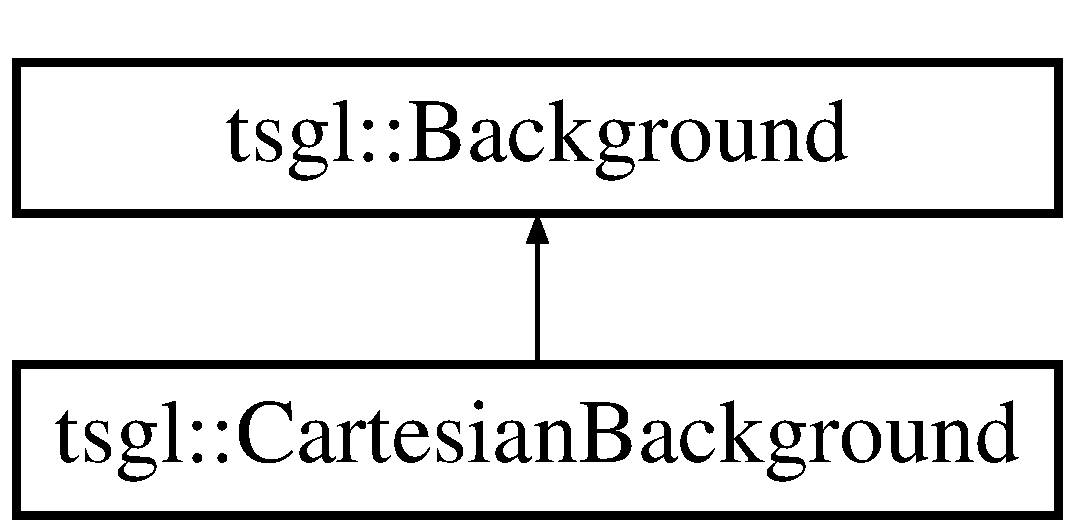
\includegraphics[height=2.000000cm]{classtsgl_1_1_cartesian_background}
\end{center}
\end{figure}
\subsection*{Public Member Functions}
\begin{DoxyCompactItemize}
\item 
\hyperlink{classtsgl_1_1_cartesian_background_aff44104863ff24b333e599e03a837318}{Cartesian\+Background} (G\+Lint width, G\+Lint height, Decimal x\+Min, Decimal y\+Min, Decimal x\+Max, Decimal y\+Max, const \hyperlink{structtsgl_1_1_color_float}{Color\+Float} \&c=W\+H\+I\+TE)
\begin{DoxyCompactList}\small\item\em Explicitly constructs a new \hyperlink{classtsgl_1_1_cartesian_background}{Cartesian\+Background}. \end{DoxyCompactList}\item 
virtual void \hyperlink{classtsgl_1_1_cartesian_background_a4cdb6866a066e6647af9dbdae738b9b2}{draw} ()
\begin{DoxyCompactList}\small\item\em Draw the \hyperlink{classtsgl_1_1_cartesian_background}{Cartesian\+Background}. \end{DoxyCompactList}\item 
virtual void \hyperlink{classtsgl_1_1_cartesian_background_ad6b87579d02c1ed138d7ace809e705a8}{draw\+Axes} (Decimal originX, Decimal originY, Decimal spacingX, Decimal spacingY)
\begin{DoxyCompactList}\small\item\em Draws axes on the Cartesian \hyperlink{classtsgl_1_1_background}{Background}. \end{DoxyCompactList}\item 
void \hyperlink{classtsgl_1_1_cartesian_background_ae494eed2e3277ddc0506d382054f22c3}{draw\+Function} (const \hyperlink{classtsgl_1_1_function}{Function} \&function, \hyperlink{structtsgl_1_1_color_float}{Color\+Float} color=B\+L\+A\+CK)
\begin{DoxyCompactList}\small\item\em Plots a function on the screen. \end{DoxyCompactList}\item 
void \hyperlink{classtsgl_1_1_cartesian_background_a8c7be40429c42d0e4504eeb6b0057a95}{draw\+Function} (function\+Pointer \&function, \hyperlink{structtsgl_1_1_color_float}{Color\+Float} color=B\+L\+A\+CK)
\begin{DoxyCompactList}\small\item\em Plots a function on the screen. \end{DoxyCompactList}\item 
void \hyperlink{classtsgl_1_1_cartesian_background_a315ee79b872d8fc612749795f4bbb6d9}{draw\+Partial\+Function} (function\+Pointer \&function, Decimal min, Decimal max, \hyperlink{structtsgl_1_1_color_float}{Color\+Float} color=B\+L\+A\+CK)
\begin{DoxyCompactList}\small\item\em Plots part of a function on the screen. \end{DoxyCompactList}\item 
virtual void \hyperlink{classtsgl_1_1_cartesian_background_a3a5a05134a9cfd0569efe2fd66d30e6a}{draw\+Pixel} (float x, float y, \hyperlink{structtsgl_1_1_color_int}{Color\+Int} c)
\begin{DoxyCompactList}\small\item\em Draws a single pixel, specified in x,y format, at the given Cartesian coordinates. \end{DoxyCompactList}\item 
Decimal \hyperlink{classtsgl_1_1_cartesian_background_a93d3f5f05ad533a5ec1f896477182aff}{get\+Cart\+Height} ()
\begin{DoxyCompactList}\small\item\em Accessor for the \hyperlink{classtsgl_1_1_cartesian_background}{Cartesian\+Background}\textquotesingle{}s Cartesian height. \end{DoxyCompactList}\item 
Decimal \hyperlink{classtsgl_1_1_cartesian_background_a7bede4180193c61fcaf01c9f3cc6aca1}{get\+Cart\+Width} ()
\begin{DoxyCompactList}\small\item\em Accessor for the \hyperlink{classtsgl_1_1_cartesian_background}{Cartesian\+Background}\textquotesingle{}s Cartesian width. \end{DoxyCompactList}\item 
Decimal \hyperlink{classtsgl_1_1_cartesian_background_af8131853b72c0ff370b1b558bf2c8073}{get\+MaxX} ()
\begin{DoxyCompactList}\small\item\em Accessor for the \hyperlink{classtsgl_1_1_cartesian_background}{Cartesian\+Background}\textquotesingle{}s right bound. \end{DoxyCompactList}\item 
Decimal \hyperlink{classtsgl_1_1_cartesian_background_a6f0d1852411eae2fe0a2822a6da29d7d}{get\+MaxY} ()
\begin{DoxyCompactList}\small\item\em Accessor for the \hyperlink{classtsgl_1_1_cartesian_background}{Cartesian\+Background}\textquotesingle{}s top bound. \end{DoxyCompactList}\item 
Decimal \hyperlink{classtsgl_1_1_cartesian_background_a8bc9825516fb188932a992a5ad6baf49}{get\+MinX} ()
\begin{DoxyCompactList}\small\item\em Accessor for the \hyperlink{classtsgl_1_1_cartesian_background}{Cartesian\+Background}\textquotesingle{}s left bound. \end{DoxyCompactList}\item 
Decimal \hyperlink{classtsgl_1_1_cartesian_background_a732052e2af266586179855eea5b45361}{get\+MinY} ()
\begin{DoxyCompactList}\small\item\em Accessor for the \hyperlink{classtsgl_1_1_cartesian_background}{Cartesian\+Background}\textquotesingle{}s bottom bound. \end{DoxyCompactList}\item 
virtual \hyperlink{structtsgl_1_1_color_int}{Color\+Int} \hyperlink{classtsgl_1_1_cartesian_background_a36a3e803d2ffe16e2e1639359f7c7be5}{get\+Pixel} (float x, float y)
\begin{DoxyCompactList}\small\item\em Gets the color of the pixel drawn on the current \hyperlink{classtsgl_1_1_background}{Background} at the given x and y Cartesian coordinates. \end{DoxyCompactList}\item 
void \hyperlink{classtsgl_1_1_cartesian_background_afd50b54bbeeace2a72e39363f76a460f}{zoom} (Decimal x, Decimal y, Decimal scale)
\begin{DoxyCompactList}\small\item\em Zoom the \hyperlink{classtsgl_1_1_cartesian_background}{Cartesian\+Background} with a given center. \end{DoxyCompactList}\item 
void \hyperlink{classtsgl_1_1_cartesian_background_a7f4464f03382151b767387a0f7befd72}{zoom} (Decimal x1, Decimal y1, Decimal x2, Decimal y2)
\begin{DoxyCompactList}\small\item\em Zoom the \hyperlink{classtsgl_1_1_cartesian_background}{Cartesian\+Background} with the given bounding (Cartesian) coordinates. \end{DoxyCompactList}\end{DoxyCompactItemize}
\subsection*{Protected Member Functions}
\begin{DoxyCompactItemize}
\item 
virtual void \hyperlink{classtsgl_1_1_cartesian_background_a3d898bf3fe826c563e74c72e93cd3c74}{select\+Shaders} (unsigned int s\+Type) override
\begin{DoxyCompactList}\small\item\em Activates the corresponding Shader for a given \hyperlink{classtsgl_1_1_drawable}{Drawable}. \end{DoxyCompactList}\end{DoxyCompactItemize}
\subsection*{Protected Attributes}
\begin{DoxyCompactItemize}
\item 
\mbox{\Hypertarget{classtsgl_1_1_cartesian_background_ab7a5f86531e3ca87a11efb8600fb4e03}\label{classtsgl_1_1_cartesian_background_ab7a5f86531e3ca87a11efb8600fb4e03}} 
Decimal {\bfseries my\+Cart\+Width}
\item 
\mbox{\Hypertarget{classtsgl_1_1_cartesian_background_ae93d4a1074cb5285406cd753733e48ed}\label{classtsgl_1_1_cartesian_background_ae93d4a1074cb5285406cd753733e48ed}} 
Decimal {\bfseries my\+Cart\+Height}
\item 
\mbox{\Hypertarget{classtsgl_1_1_cartesian_background_a0d22e13bc40c8d99103170d9386d5de8}\label{classtsgl_1_1_cartesian_background_a0d22e13bc40c8d99103170d9386d5de8}} 
Decimal {\bfseries my\+X\+Min}
\item 
\mbox{\Hypertarget{classtsgl_1_1_cartesian_background_add335e91ed82c520b28369cd93067618}\label{classtsgl_1_1_cartesian_background_add335e91ed82c520b28369cd93067618}} 
Decimal {\bfseries my\+X\+Max}
\item 
\mbox{\Hypertarget{classtsgl_1_1_cartesian_background_a16510f597bc529fbc2e96bce3d7bbac5}\label{classtsgl_1_1_cartesian_background_a16510f597bc529fbc2e96bce3d7bbac5}} 
Decimal {\bfseries my\+Y\+Min}
\item 
\mbox{\Hypertarget{classtsgl_1_1_cartesian_background_a3afa7fc438538c504347349d9ff8d85c}\label{classtsgl_1_1_cartesian_background_a3afa7fc438538c504347349d9ff8d85c}} 
Decimal {\bfseries my\+Y\+Max}
\item 
\mbox{\Hypertarget{classtsgl_1_1_cartesian_background_a1c44de7a723be16561717eec0afb7916}\label{classtsgl_1_1_cartesian_background_a1c44de7a723be16561717eec0afb7916}} 
Decimal {\bfseries pixel\+Width}
\item 
\mbox{\Hypertarget{classtsgl_1_1_cartesian_background_a0d1f3d876b9876467691498a28e1fcce}\label{classtsgl_1_1_cartesian_background_a0d1f3d876b9876467691498a28e1fcce}} 
Decimal {\bfseries pixel\+Height}
\end{DoxyCompactItemize}


\subsection{Detailed Description}
Draw a procedurally drawn \hyperlink{classtsgl_1_1_cartesian_background}{Cartesian\+Background} for the \hyperlink{classtsgl_1_1_canvas}{Canvas}. 

\hyperlink{classtsgl_1_1_cartesian_background}{Cartesian\+Background} is a class for holding a framebuffer of color data. 

\subsection{Constructor \& Destructor Documentation}
\mbox{\Hypertarget{classtsgl_1_1_cartesian_background_aff44104863ff24b333e599e03a837318}\label{classtsgl_1_1_cartesian_background_aff44104863ff24b333e599e03a837318}} 
\index{tsgl\+::\+Cartesian\+Background@{tsgl\+::\+Cartesian\+Background}!Cartesian\+Background@{Cartesian\+Background}}
\index{Cartesian\+Background@{Cartesian\+Background}!tsgl\+::\+Cartesian\+Background@{tsgl\+::\+Cartesian\+Background}}
\subsubsection{\texorpdfstring{Cartesian\+Background()}{CartesianBackground()}}
{\footnotesize\ttfamily tsgl\+::\+Cartesian\+Background\+::\+Cartesian\+Background (\begin{DoxyParamCaption}\item[{G\+Lint}]{width,  }\item[{G\+Lint}]{height,  }\item[{Decimal}]{x\+Min,  }\item[{Decimal}]{y\+Min,  }\item[{Decimal}]{x\+Max,  }\item[{Decimal}]{y\+Max,  }\item[{const \hyperlink{structtsgl_1_1_color_float}{Color\+Float} \&}]{clear\+Color = {\ttfamily WHITE} }\end{DoxyParamCaption})}



Explicitly constructs a new \hyperlink{classtsgl_1_1_cartesian_background}{Cartesian\+Background}. 

Creates a \hyperlink{classtsgl_1_1_background}{Background} whose world dimensions don\textquotesingle{}t have to match its pixel dimensions. 
\begin{DoxyParams}{Parameters}
{\em width} & \hyperlink{classtsgl_1_1_cartesian_background}{Cartesian\+Background}\textquotesingle{}s width in pixels. \\
\hline
{\em height} & \hyperlink{classtsgl_1_1_cartesian_background}{Cartesian\+Background}\textquotesingle{}s height in pixels. \\
\hline
{\em x\+Min} & x value of the left side of the \hyperlink{classtsgl_1_1_cartesian_background}{Cartesian\+Background} in world coordinates. \\
\hline
{\em x\+Max} & x value of the right side of the \hyperlink{classtsgl_1_1_cartesian_background}{Cartesian\+Background} in world coordinates. \\
\hline
{\em y\+Min} & y value of the bottom side of the \hyperlink{classtsgl_1_1_cartesian_background}{Cartesian\+Background} in world coordinates. \\
\hline
{\em y\+Max} & y value of the top side of the \hyperlink{classtsgl_1_1_cartesian_background}{Cartesian\+Background} in world coordinates. \\
\hline
{\em c} & A \hyperlink{structtsgl_1_1_color_float}{Color\+Float} for the \hyperlink{classtsgl_1_1_cartesian_background}{Cartesian\+Background}\textquotesingle{}s original color. \\
\hline
\end{DoxyParams}
\begin{DoxyWarning}{Warning}
An invariant is held where if x\+Max or x\+Min isn\textquotesingle{}t greater than its respective min then an error message is given. 
\end{DoxyWarning}
\begin{DoxyReturn}{Returns}
A new \hyperlink{classtsgl_1_1_cartesian_background}{Cartesian\+Background} to which Drawables and Pixels can be drawn procedurally. 
\end{DoxyReturn}


\subsection{Member Function Documentation}
\mbox{\Hypertarget{classtsgl_1_1_cartesian_background_a4cdb6866a066e6647af9dbdae738b9b2}\label{classtsgl_1_1_cartesian_background_a4cdb6866a066e6647af9dbdae738b9b2}} 
\index{tsgl\+::\+Cartesian\+Background@{tsgl\+::\+Cartesian\+Background}!draw@{draw}}
\index{draw@{draw}!tsgl\+::\+Cartesian\+Background@{tsgl\+::\+Cartesian\+Background}}
\subsubsection{\texorpdfstring{draw()}{draw()}}
{\footnotesize\ttfamily void tsgl\+::\+Cartesian\+Background\+::draw (\begin{DoxyParamCaption}{ }\end{DoxyParamCaption})\hspace{0.3cm}{\ttfamily [virtual]}}



Draw the \hyperlink{classtsgl_1_1_cartesian_background}{Cartesian\+Background}. 

This function actually draws the \hyperlink{classtsgl_1_1_cartesian_background}{Cartesian\+Background} to the \hyperlink{classtsgl_1_1_canvas}{Canvas}. \begin{DoxyNote}{Note}
On each draw cycle, first any Drawables that have been newly added to the \hyperlink{classtsgl_1_1_cartesian_background}{Cartesian\+Background} will be rendered, and then any new calls to draw\+Pixel will be processed. 
\end{DoxyNote}


Reimplemented from \hyperlink{classtsgl_1_1_background_a62314d455c7b09b2686ba46fd1e5c663}{tsgl\+::\+Background}.

\mbox{\Hypertarget{classtsgl_1_1_cartesian_background_ad6b87579d02c1ed138d7ace809e705a8}\label{classtsgl_1_1_cartesian_background_ad6b87579d02c1ed138d7ace809e705a8}} 
\index{tsgl\+::\+Cartesian\+Background@{tsgl\+::\+Cartesian\+Background}!draw\+Axes@{draw\+Axes}}
\index{draw\+Axes@{draw\+Axes}!tsgl\+::\+Cartesian\+Background@{tsgl\+::\+Cartesian\+Background}}
\subsubsection{\texorpdfstring{draw\+Axes()}{drawAxes()}}
{\footnotesize\ttfamily void tsgl\+::\+Cartesian\+Background\+::draw\+Axes (\begin{DoxyParamCaption}\item[{Decimal}]{originX,  }\item[{Decimal}]{originY,  }\item[{Decimal}]{spacingX,  }\item[{Decimal}]{spacingY }\end{DoxyParamCaption})\hspace{0.3cm}{\ttfamily [virtual]}}



Draws axes on the Cartesian \hyperlink{classtsgl_1_1_background}{Background}. 

This function draws axes (with tick marks) on the \hyperlink{classtsgl_1_1_cartesian_background}{Cartesian\+Background}, centered at the given (Cartesian) coordinates 
\begin{DoxyParams}{Parameters}
{\em originX} & The horizontal location of the y-\/axis line. \\
\hline
{\em originY} & The vertical location of the x-\/axis line. \\
\hline
{\em spacingX} & The distance between marks on the x-\/axis. \\
\hline
{\em spacingY} & The distance between marks on the y-\/axis. \\
\hline
\end{DoxyParams}


Referenced by tsgl\+::\+Integral\+Viewer\+::$\sim$\+Integral\+Viewer().

\mbox{\Hypertarget{classtsgl_1_1_cartesian_background_ae494eed2e3277ddc0506d382054f22c3}\label{classtsgl_1_1_cartesian_background_ae494eed2e3277ddc0506d382054f22c3}} 
\index{tsgl\+::\+Cartesian\+Background@{tsgl\+::\+Cartesian\+Background}!draw\+Function@{draw\+Function}}
\index{draw\+Function@{draw\+Function}!tsgl\+::\+Cartesian\+Background@{tsgl\+::\+Cartesian\+Background}}
\subsubsection{\texorpdfstring{draw\+Function()}{drawFunction()}\hspace{0.1cm}{\footnotesize\ttfamily [1/2]}}
{\footnotesize\ttfamily void tsgl\+::\+Cartesian\+Background\+::draw\+Function (\begin{DoxyParamCaption}\item[{const \hyperlink{classtsgl_1_1_function}{Function} \&}]{function,  }\item[{\hyperlink{structtsgl_1_1_color_float}{Color\+Float}}]{color = {\ttfamily BLACK} }\end{DoxyParamCaption})}



Plots a function on the screen. 

This function receives a T\+S\+GL \hyperlink{classtsgl_1_1_function}{Function} instance as a parameter and plots the function on the \hyperlink{classtsgl_1_1_cartesian_canvas}{Cartesian\+Canvas}. 
\begin{DoxyParams}{Parameters}
{\em function} & Reference to the \hyperlink{classtsgl_1_1_function}{Function} to plot. \\
\hline
{\em color} & The color of the vertices of the plotted function (set to B\+L\+A\+CK by default). \\
\hline
\end{DoxyParams}
\mbox{\Hypertarget{classtsgl_1_1_cartesian_background_a8c7be40429c42d0e4504eeb6b0057a95}\label{classtsgl_1_1_cartesian_background_a8c7be40429c42d0e4504eeb6b0057a95}} 
\index{tsgl\+::\+Cartesian\+Background@{tsgl\+::\+Cartesian\+Background}!draw\+Function@{draw\+Function}}
\index{draw\+Function@{draw\+Function}!tsgl\+::\+Cartesian\+Background@{tsgl\+::\+Cartesian\+Background}}
\subsubsection{\texorpdfstring{draw\+Function()}{drawFunction()}\hspace{0.1cm}{\footnotesize\ttfamily [2/2]}}
{\footnotesize\ttfamily void tsgl\+::\+Cartesian\+Background\+::draw\+Function (\begin{DoxyParamCaption}\item[{function\+Pointer \&}]{function,  }\item[{\hyperlink{structtsgl_1_1_color_float}{Color\+Float}}]{color = {\ttfamily BLACK} }\end{DoxyParamCaption})}



Plots a function on the screen. 

This function receives a pointer to a function method as a parameter and plots the function on the \hyperlink{classtsgl_1_1_cartesian_canvas}{Cartesian\+Canvas}. 
\begin{DoxyParams}{Parameters}
{\em function} & Pointer to the function-\/drawing method to plot. \\
\hline
{\em color} & The color of the vertices of the plotted function (set to B\+L\+A\+CK by default). \\
\hline
\end{DoxyParams}
\begin{DoxyNote}{Note}
{\ttfamily function} must receive exactly one Decimal x parameter, and return a Decimal y parameter. 
\end{DoxyNote}
\mbox{\Hypertarget{classtsgl_1_1_cartesian_background_a315ee79b872d8fc612749795f4bbb6d9}\label{classtsgl_1_1_cartesian_background_a315ee79b872d8fc612749795f4bbb6d9}} 
\index{tsgl\+::\+Cartesian\+Background@{tsgl\+::\+Cartesian\+Background}!draw\+Partial\+Function@{draw\+Partial\+Function}}
\index{draw\+Partial\+Function@{draw\+Partial\+Function}!tsgl\+::\+Cartesian\+Background@{tsgl\+::\+Cartesian\+Background}}
\subsubsection{\texorpdfstring{draw\+Partial\+Function()}{drawPartialFunction()}}
{\footnotesize\ttfamily void tsgl\+::\+Cartesian\+Background\+::draw\+Partial\+Function (\begin{DoxyParamCaption}\item[{function\+Pointer \&}]{function,  }\item[{Decimal}]{min,  }\item[{Decimal}]{max,  }\item[{\hyperlink{structtsgl_1_1_color_float}{Color\+Float}}]{color = {\ttfamily BLACK} }\end{DoxyParamCaption})}



Plots part of a function on the screen. 

This function receives a pointer to a function method as a parameter and plots the function on the \hyperlink{classtsgl_1_1_cartesian_canvas}{Cartesian\+Canvas} between the specified minimum and maximum coordinates. 
\begin{DoxyParams}{Parameters}
{\em function} & Pointer to the function-\/drawing method to plot. \\
\hline
{\em min} & Minimum x value to evaluate and plot \\
\hline
{\em max} & Maximum x value to evaluate and plot \\
\hline
{\em color} & The color of the vertices of the plotted function (set to B\+L\+A\+CK by default). \\
\hline
\end{DoxyParams}
\begin{DoxyNote}{Note}
{\ttfamily function} must receive exactly one Decimal x parameter, and return a Decimal y parameter. 
\end{DoxyNote}


Referenced by draw\+Function(), and tsgl\+::\+Integral\+Viewer\+::$\sim$\+Integral\+Viewer().

\mbox{\Hypertarget{classtsgl_1_1_cartesian_background_a3a5a05134a9cfd0569efe2fd66d30e6a}\label{classtsgl_1_1_cartesian_background_a3a5a05134a9cfd0569efe2fd66d30e6a}} 
\index{tsgl\+::\+Cartesian\+Background@{tsgl\+::\+Cartesian\+Background}!draw\+Pixel@{draw\+Pixel}}
\index{draw\+Pixel@{draw\+Pixel}!tsgl\+::\+Cartesian\+Background@{tsgl\+::\+Cartesian\+Background}}
\subsubsection{\texorpdfstring{draw\+Pixel()}{drawPixel()}}
{\footnotesize\ttfamily void tsgl\+::\+Cartesian\+Background\+::draw\+Pixel (\begin{DoxyParamCaption}\item[{float}]{x,  }\item[{float}]{y,  }\item[{\hyperlink{structtsgl_1_1_color_int}{Color\+Int}}]{c }\end{DoxyParamCaption})\hspace{0.3cm}{\ttfamily [virtual]}}



Draws a single pixel, specified in x,y format, at the given Cartesian coordinates. 

This function alters the value at the specified x, y offset within the \hyperlink{classtsgl_1_1_background}{Background}\textquotesingle{}s buffer variable. \begin{DoxyNote}{Note}
x and y must be given in world (Cartesian coordinates). 
\end{DoxyNote}

\begin{DoxyParams}{Parameters}
{\em x} & The Cartesian x-\/position of the pixel. \\
\hline
{\em y} & The Cartesian y-\/position of the pixel. \\
\hline
{\em color} & The color of the point. \\
\hline
\end{DoxyParams}


Reimplemented from \hyperlink{classtsgl_1_1_background_acfeec27c6bcc851652725ddd9cc3d3c9}{tsgl\+::\+Background}.



Referenced by Julia\+::draw(), Nova\+::draw(), Gradient\+Mandelbrot\+::draw(), and Mandelbrot\+::draw().

\mbox{\Hypertarget{classtsgl_1_1_cartesian_background_a93d3f5f05ad533a5ec1f896477182aff}\label{classtsgl_1_1_cartesian_background_a93d3f5f05ad533a5ec1f896477182aff}} 
\index{tsgl\+::\+Cartesian\+Background@{tsgl\+::\+Cartesian\+Background}!get\+Cart\+Height@{get\+Cart\+Height}}
\index{get\+Cart\+Height@{get\+Cart\+Height}!tsgl\+::\+Cartesian\+Background@{tsgl\+::\+Cartesian\+Background}}
\subsubsection{\texorpdfstring{get\+Cart\+Height()}{getCartHeight()}}
{\footnotesize\ttfamily Decimal tsgl\+::\+Cartesian\+Background\+::get\+Cart\+Height (\begin{DoxyParamCaption}{ }\end{DoxyParamCaption})\hspace{0.3cm}{\ttfamily [inline]}}



Accessor for the \hyperlink{classtsgl_1_1_cartesian_background}{Cartesian\+Background}\textquotesingle{}s Cartesian height. 

\begin{DoxyReturn}{Returns}
The Cartesian height of the \hyperlink{classtsgl_1_1_cartesian_background}{Cartesian\+Background}. 
\end{DoxyReturn}
\mbox{\Hypertarget{classtsgl_1_1_cartesian_background_a7bede4180193c61fcaf01c9f3cc6aca1}\label{classtsgl_1_1_cartesian_background_a7bede4180193c61fcaf01c9f3cc6aca1}} 
\index{tsgl\+::\+Cartesian\+Background@{tsgl\+::\+Cartesian\+Background}!get\+Cart\+Width@{get\+Cart\+Width}}
\index{get\+Cart\+Width@{get\+Cart\+Width}!tsgl\+::\+Cartesian\+Background@{tsgl\+::\+Cartesian\+Background}}
\subsubsection{\texorpdfstring{get\+Cart\+Width()}{getCartWidth()}}
{\footnotesize\ttfamily Decimal tsgl\+::\+Cartesian\+Background\+::get\+Cart\+Width (\begin{DoxyParamCaption}{ }\end{DoxyParamCaption})\hspace{0.3cm}{\ttfamily [inline]}}



Accessor for the \hyperlink{classtsgl_1_1_cartesian_background}{Cartesian\+Background}\textquotesingle{}s Cartesian width. 

\begin{DoxyReturn}{Returns}
The Cartesian width of the \hyperlink{classtsgl_1_1_cartesian_background}{Cartesian\+Background}. 
\end{DoxyReturn}
\mbox{\Hypertarget{classtsgl_1_1_cartesian_background_af8131853b72c0ff370b1b558bf2c8073}\label{classtsgl_1_1_cartesian_background_af8131853b72c0ff370b1b558bf2c8073}} 
\index{tsgl\+::\+Cartesian\+Background@{tsgl\+::\+Cartesian\+Background}!get\+MaxX@{get\+MaxX}}
\index{get\+MaxX@{get\+MaxX}!tsgl\+::\+Cartesian\+Background@{tsgl\+::\+Cartesian\+Background}}
\subsubsection{\texorpdfstring{get\+Max\+X()}{getMaxX()}}
{\footnotesize\ttfamily Decimal tsgl\+::\+Cartesian\+Background\+::get\+MaxX (\begin{DoxyParamCaption}{ }\end{DoxyParamCaption})\hspace{0.3cm}{\ttfamily [inline]}}



Accessor for the \hyperlink{classtsgl_1_1_cartesian_background}{Cartesian\+Background}\textquotesingle{}s right bound. 

\begin{DoxyReturn}{Returns}
The real number corresponding the right of the \hyperlink{classtsgl_1_1_cartesian_background}{Cartesian\+Background}. 
\end{DoxyReturn}


Referenced by Mandelbrot\+::draw().

\mbox{\Hypertarget{classtsgl_1_1_cartesian_background_a6f0d1852411eae2fe0a2822a6da29d7d}\label{classtsgl_1_1_cartesian_background_a6f0d1852411eae2fe0a2822a6da29d7d}} 
\index{tsgl\+::\+Cartesian\+Background@{tsgl\+::\+Cartesian\+Background}!get\+MaxY@{get\+MaxY}}
\index{get\+MaxY@{get\+MaxY}!tsgl\+::\+Cartesian\+Background@{tsgl\+::\+Cartesian\+Background}}
\subsubsection{\texorpdfstring{get\+Max\+Y()}{getMaxY()}}
{\footnotesize\ttfamily Decimal tsgl\+::\+Cartesian\+Background\+::get\+MaxY (\begin{DoxyParamCaption}{ }\end{DoxyParamCaption})\hspace{0.3cm}{\ttfamily [inline]}}



Accessor for the \hyperlink{classtsgl_1_1_cartesian_background}{Cartesian\+Background}\textquotesingle{}s top bound. 

\begin{DoxyReturn}{Returns}
The real number corresponding the top of the \hyperlink{classtsgl_1_1_cartesian_background}{Cartesian\+Background}. 
\end{DoxyReturn}
\mbox{\Hypertarget{classtsgl_1_1_cartesian_background_a8bc9825516fb188932a992a5ad6baf49}\label{classtsgl_1_1_cartesian_background_a8bc9825516fb188932a992a5ad6baf49}} 
\index{tsgl\+::\+Cartesian\+Background@{tsgl\+::\+Cartesian\+Background}!get\+MinX@{get\+MinX}}
\index{get\+MinX@{get\+MinX}!tsgl\+::\+Cartesian\+Background@{tsgl\+::\+Cartesian\+Background}}
\subsubsection{\texorpdfstring{get\+Min\+X()}{getMinX()}}
{\footnotesize\ttfamily Decimal tsgl\+::\+Cartesian\+Background\+::get\+MinX (\begin{DoxyParamCaption}{ }\end{DoxyParamCaption})\hspace{0.3cm}{\ttfamily [inline]}}



Accessor for the \hyperlink{classtsgl_1_1_cartesian_background}{Cartesian\+Background}\textquotesingle{}s left bound. 

\begin{DoxyReturn}{Returns}
The real number corresponding the left of the \hyperlink{classtsgl_1_1_cartesian_background}{Cartesian\+Background}. 
\end{DoxyReturn}


Referenced by Mandelbrot\+::draw().

\mbox{\Hypertarget{classtsgl_1_1_cartesian_background_a732052e2af266586179855eea5b45361}\label{classtsgl_1_1_cartesian_background_a732052e2af266586179855eea5b45361}} 
\index{tsgl\+::\+Cartesian\+Background@{tsgl\+::\+Cartesian\+Background}!get\+MinY@{get\+MinY}}
\index{get\+MinY@{get\+MinY}!tsgl\+::\+Cartesian\+Background@{tsgl\+::\+Cartesian\+Background}}
\subsubsection{\texorpdfstring{get\+Min\+Y()}{getMinY()}}
{\footnotesize\ttfamily Decimal tsgl\+::\+Cartesian\+Background\+::get\+MinY (\begin{DoxyParamCaption}{ }\end{DoxyParamCaption})\hspace{0.3cm}{\ttfamily [inline]}}



Accessor for the \hyperlink{classtsgl_1_1_cartesian_background}{Cartesian\+Background}\textquotesingle{}s bottom bound. 

\begin{DoxyReturn}{Returns}
The real number corresponding the bottom of the \hyperlink{classtsgl_1_1_cartesian_background}{Cartesian\+Background}. 
\end{DoxyReturn}
\mbox{\Hypertarget{classtsgl_1_1_cartesian_background_a36a3e803d2ffe16e2e1639359f7c7be5}\label{classtsgl_1_1_cartesian_background_a36a3e803d2ffe16e2e1639359f7c7be5}} 
\index{tsgl\+::\+Cartesian\+Background@{tsgl\+::\+Cartesian\+Background}!get\+Pixel@{get\+Pixel}}
\index{get\+Pixel@{get\+Pixel}!tsgl\+::\+Cartesian\+Background@{tsgl\+::\+Cartesian\+Background}}
\subsubsection{\texorpdfstring{get\+Pixel()}{getPixel()}}
{\footnotesize\ttfamily \hyperlink{structtsgl_1_1_color_int}{Color\+Int} tsgl\+::\+Cartesian\+Background\+::get\+Pixel (\begin{DoxyParamCaption}\item[{float}]{x,  }\item[{float}]{y }\end{DoxyParamCaption})\hspace{0.3cm}{\ttfamily [virtual]}}



Gets the color of the pixel drawn on the current \hyperlink{classtsgl_1_1_background}{Background} at the given x and y Cartesian coordinates. 

\begin{DoxyNote}{Note}
x and y must be given in world (Cartesian coordinates). 
\end{DoxyNote}

\begin{DoxyParams}{Parameters}
{\em x} & The Cartesian x-\/position of the pixel to grab. \\
\hline
{\em y} & The Cartesian y-\/position of the pixel to grab. \\
\hline
\end{DoxyParams}
\begin{DoxyReturn}{Returns}
A \hyperlink{structtsgl_1_1_color_int}{Color\+Int} containing the color of the pixel at (x,y). 
\end{DoxyReturn}


Reimplemented from \hyperlink{classtsgl_1_1_background_a09d91731095fd0839eaf6e46c3d279b5}{tsgl\+::\+Background}.



Referenced by get\+Min\+Y().

\mbox{\Hypertarget{classtsgl_1_1_cartesian_background_a3d898bf3fe826c563e74c72e93cd3c74}\label{classtsgl_1_1_cartesian_background_a3d898bf3fe826c563e74c72e93cd3c74}} 
\index{tsgl\+::\+Cartesian\+Background@{tsgl\+::\+Cartesian\+Background}!select\+Shaders@{select\+Shaders}}
\index{select\+Shaders@{select\+Shaders}!tsgl\+::\+Cartesian\+Background@{tsgl\+::\+Cartesian\+Background}}
\subsubsection{\texorpdfstring{select\+Shaders()}{selectShaders()}}
{\footnotesize\ttfamily void tsgl\+::\+Cartesian\+Background\+::select\+Shaders (\begin{DoxyParamCaption}\item[{unsigned int}]{s\+Type }\end{DoxyParamCaption})\hspace{0.3cm}{\ttfamily [override]}, {\ttfamily [protected]}, {\ttfamily [virtual]}}



Activates the corresponding Shader for a given \hyperlink{classtsgl_1_1_drawable}{Drawable}. 


\begin{DoxyParams}{Parameters}
{\em s\+Type} & Unsigned int with a corresponding value for each type of Shader. \\
\hline
\end{DoxyParams}


Reimplemented from \hyperlink{classtsgl_1_1_background_a5207bcb45daafed4d6a739a8a0a0829e}{tsgl\+::\+Background}.



Referenced by draw().

\mbox{\Hypertarget{classtsgl_1_1_cartesian_background_afd50b54bbeeace2a72e39363f76a460f}\label{classtsgl_1_1_cartesian_background_afd50b54bbeeace2a72e39363f76a460f}} 
\index{tsgl\+::\+Cartesian\+Background@{tsgl\+::\+Cartesian\+Background}!zoom@{zoom}}
\index{zoom@{zoom}!tsgl\+::\+Cartesian\+Background@{tsgl\+::\+Cartesian\+Background}}
\subsubsection{\texorpdfstring{zoom()}{zoom()}\hspace{0.1cm}{\footnotesize\ttfamily [1/2]}}
{\footnotesize\ttfamily void tsgl\+::\+Cartesian\+Background\+::zoom (\begin{DoxyParamCaption}\item[{Decimal}]{x,  }\item[{Decimal}]{y,  }\item[{Decimal}]{scale }\end{DoxyParamCaption})}



Zoom the \hyperlink{classtsgl_1_1_cartesian_background}{Cartesian\+Background} with a given center. 

This function will re-\/center the \hyperlink{classtsgl_1_1_cartesian_background}{Cartesian\+Background} at the given coordinates, then zoom with respect to the given scale. 
\begin{DoxyParams}{Parameters}
{\em x} & The coordinate to re-\/center the screen on. \\
\hline
{\em y} & The coordinate to re-\/center the screen on. \\
\hline
{\em scale} & The zoom scale compared to the original. Less than 1 zooms in, greater than 1 zooms out. \\
\hline
\end{DoxyParams}
\begin{DoxyNote}{Note}
This function will automatically maintain the current aspect ratio. 
\end{DoxyNote}


Referenced by get\+Min\+Y(), zoom(), and tsgl\+::\+Cartesian\+Canvas\+::zoom().

\mbox{\Hypertarget{classtsgl_1_1_cartesian_background_a7f4464f03382151b767387a0f7befd72}\label{classtsgl_1_1_cartesian_background_a7f4464f03382151b767387a0f7befd72}} 
\index{tsgl\+::\+Cartesian\+Background@{tsgl\+::\+Cartesian\+Background}!zoom@{zoom}}
\index{zoom@{zoom}!tsgl\+::\+Cartesian\+Background@{tsgl\+::\+Cartesian\+Background}}
\subsubsection{\texorpdfstring{zoom()}{zoom()}\hspace{0.1cm}{\footnotesize\ttfamily [2/2]}}
{\footnotesize\ttfamily void tsgl\+::\+Cartesian\+Background\+::zoom (\begin{DoxyParamCaption}\item[{Decimal}]{x1,  }\item[{Decimal}]{y1,  }\item[{Decimal}]{x2,  }\item[{Decimal}]{y2 }\end{DoxyParamCaption})}



Zoom the \hyperlink{classtsgl_1_1_cartesian_background}{Cartesian\+Background} with the given bounding (Cartesian) coordinates. 

This function will zoom the \hyperlink{classtsgl_1_1_cartesian_background}{Cartesian\+Background} with respect to the given bounding coordinates. 
\begin{DoxyParams}{Parameters}
{\em x1} & The left Cartesian bound. \\
\hline
{\em y1} & The bottom Cartesian bound. \\
\hline
{\em x2} & The right Cartesian bound. \\
\hline
{\em y2} & The top Cartesian bound. \\
\hline
\end{DoxyParams}
\begin{DoxyNote}{Note}
Setting the right bound lower than the left bound or the top lower than the bottom will just swap the variables. 
\end{DoxyNote}
\begin{DoxyWarning}{Warning}
This function will {\itshape N\+OT} automatically maintain the previous aspect ratio. 

Change the aspect ratio on-\/the-\/fly only with caution. 
\end{DoxyWarning}


The documentation for this class was generated from the following files\+:\begin{DoxyCompactItemize}
\item 
Cartesian\+Background.\+h\item 
Cartesian\+Background.\+cpp\end{DoxyCompactItemize}

\hypertarget{classtsgl_1_1_cartesian_canvas}{}\section{tsgl\+:\+:Cartesian\+Canvas Class Reference}
\label{classtsgl_1_1_cartesian_canvas}\index{tsgl\+::\+Cartesian\+Canvas@{tsgl\+::\+Cartesian\+Canvas}}


\hyperlink{classtsgl_1_1_canvas}{Canvas} extended for graphic support.  




{\ttfamily \#include $<$Cartesian\+Canvas.\+h$>$}

Inheritance diagram for tsgl\+:\+:Cartesian\+Canvas\+:\begin{figure}[H]
\begin{center}
\leavevmode
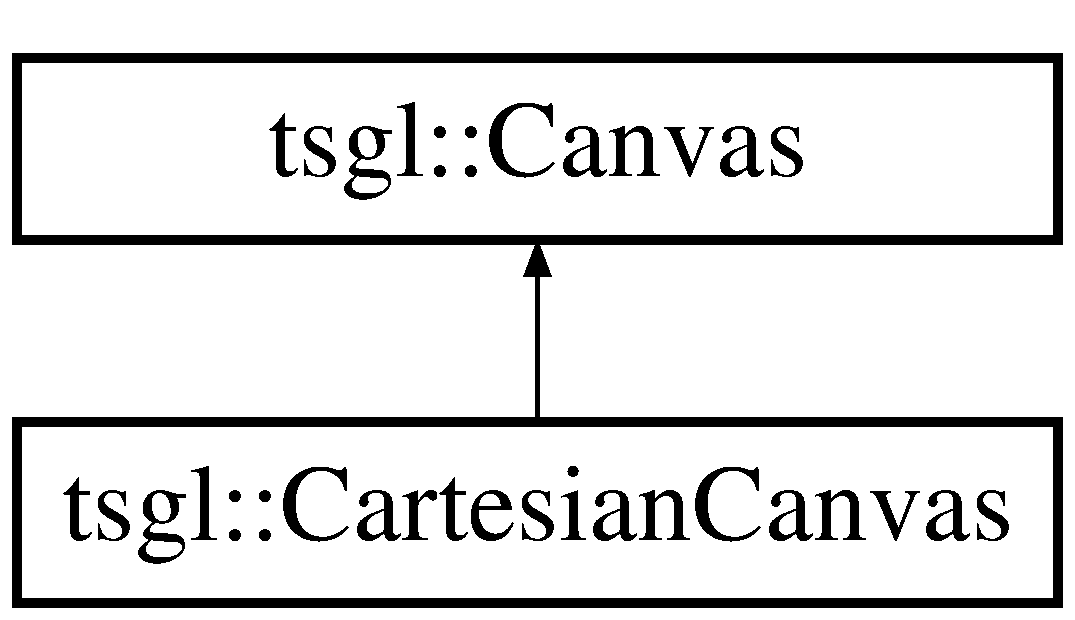
\includegraphics[height=2.000000cm]{classtsgl_1_1_cartesian_canvas}
\end{center}
\end{figure}
\subsection*{Public Member Functions}
\begin{DoxyCompactItemize}
\item 
\hyperlink{classtsgl_1_1_cartesian_canvas_a4438f368eae3def6a70e0faa15d28daa}{Cartesian\+Canvas} (double timer\+Length=0.\+0)
\begin{DoxyCompactList}\small\item\em Default \hyperlink{classtsgl_1_1_cartesian_canvas}{Cartesian\+Canvas} constructor method. \end{DoxyCompactList}\item 
\hyperlink{classtsgl_1_1_cartesian_canvas_a7ca80bfa69d89fdbe110a7ec3aa6f100}{Cartesian\+Canvas} (int x, int y, int width, int height, Decimal x\+Min, Decimal y\+Min, Decimal x\+Max, Decimal y\+Max, std\+::string t, double timer\+Length=0.\+0)
\begin{DoxyCompactList}\small\item\em Explicit \hyperlink{classtsgl_1_1_cartesian_canvas}{Cartesian\+Canvas} constructor method. \end{DoxyCompactList}\item 
void \hyperlink{classtsgl_1_1_cartesian_canvas_a1b08e3c0d692603fd2bf56e38eb19907}{draw\+Axes} (Decimal origin\+X, Decimal origin\+Y, Decimal spacing\+X, Decimal spacing\+Y)
\begin{DoxyCompactList}\small\item\em Draws axes on the Cartesian \hyperlink{classtsgl_1_1_canvas}{Canvas}. \end{DoxyCompactList}\item 
void \hyperlink{classtsgl_1_1_cartesian_canvas_a64e128195cbcf9b60dbe478d6f489d67}{draw\+Circle} (Decimal x, Decimal y, Decimal radius, int sides, \hyperlink{structtsgl_1_1_color_float}{Color\+Float} color=B\+L\+A\+C\+K, bool filled=true)
\begin{DoxyCompactList}\small\item\em Draws a circle. \end{DoxyCompactList}\item 
void \hyperlink{classtsgl_1_1_cartesian_canvas_a169f867f6b0d0706dca96a1f4fcc0172}{draw\+Colored\+Polygon} (int size, Decimal xverts\mbox{[}$\,$\mbox{]}, Decimal yverts\mbox{[}$\,$\mbox{]}, \hyperlink{structtsgl_1_1_color_float}{Color\+Float} color\mbox{[}$\,$\mbox{]}, bool filled=true)
\begin{DoxyCompactList}\small\item\em Draws an arbitrary polygon with colored vertices. \end{DoxyCompactList}\item 
void \hyperlink{classtsgl_1_1_cartesian_canvas_a7f84b79ab6fd77277c5c71fce7d0ec6a}{draw\+Concave\+Polygon} (int size, Decimal xverts\mbox{[}$\,$\mbox{]}, Decimal yverts\mbox{[}$\,$\mbox{]}, \hyperlink{structtsgl_1_1_color_float}{Color\+Float} color\mbox{[}$\,$\mbox{]}, bool filled=true)
\begin{DoxyCompactList}\small\item\em Draws a Concave polygon with colored vertices. \end{DoxyCompactList}\item 
void \hyperlink{classtsgl_1_1_cartesian_canvas_abefc7f373711cdff2477d0665b37212f}{draw\+Convex\+Polygon} (int size, Decimal xverts\mbox{[}$\,$\mbox{]}, Decimal yverts\mbox{[}$\,$\mbox{]}, \hyperlink{structtsgl_1_1_color_float}{Color\+Float} color\mbox{[}$\,$\mbox{]}, bool filled=true)
\begin{DoxyCompactList}\small\item\em Draws a convex polygon with colored vertices. \end{DoxyCompactList}\item 
void \hyperlink{classtsgl_1_1_cartesian_canvas_aa2da030609cf410eecfc154fd67491cf}{draw\+Function} (const \hyperlink{classtsgl_1_1_function}{Function} \&function, \hyperlink{structtsgl_1_1_color_float}{Color\+Float} color=B\+L\+A\+C\+K)
\begin{DoxyCompactList}\small\item\em Plots a function on the screen. \end{DoxyCompactList}\item 
void \hyperlink{classtsgl_1_1_cartesian_canvas_ab2f3e7633f4f05711083eba01b0a3f4e}{draw\+Image} (std\+::string filename, Decimal x, Decimal y, Decimal w, Decimal h, float a=1.\+0f)
\begin{DoxyCompactList}\small\item\em Draws an image. \end{DoxyCompactList}\item 
void \hyperlink{classtsgl_1_1_cartesian_canvas_ace015a630f1ff280b2ecd6a864cdc5e2}{draw\+Line} (Decimal x1, Decimal y1, Decimal x2, Decimal y2, \hyperlink{structtsgl_1_1_color_float}{Color\+Float} color=B\+L\+A\+C\+K)
\begin{DoxyCompactList}\small\item\em Draws a line. \end{DoxyCompactList}\item 
void \hyperlink{classtsgl_1_1_cartesian_canvas_a2ef932501dd03f885fd0ff30ddffae01}{draw\+Point} (Decimal x, Decimal y, \hyperlink{structtsgl_1_1_color_float}{Color\+Float} color=B\+L\+A\+C\+K)
\begin{DoxyCompactList}\small\item\em Draws a single pixel, specified in x,y format. \end{DoxyCompactList}\item 
void \hyperlink{classtsgl_1_1_cartesian_canvas_a5e88e7d751e24ae78d158f1d8e9faf5e}{draw\+Rectangle} (Decimal x1, Decimal y1, Decimal x2, Decimal y2, \hyperlink{structtsgl_1_1_color_float}{Color\+Float} color=B\+L\+A\+C\+K, bool filled=true)
\begin{DoxyCompactList}\small\item\em Draws a rectangle. \end{DoxyCompactList}\item 
void \hyperlink{classtsgl_1_1_cartesian_canvas_a7df01e80ce99d0ce6b45532034c0940c}{draw\+Text} (std\+::string text, Decimal x, Decimal y, unsigned size, \hyperlink{structtsgl_1_1_color_float}{Color\+Float} color=B\+L\+A\+C\+K)
\begin{DoxyCompactList}\small\item\em Draw a string of text. \end{DoxyCompactList}\item 
void \hyperlink{classtsgl_1_1_cartesian_canvas_addacb4d3637bf2674e2a992a0c165160}{draw\+Text} (std\+::wstring text, Decimal x, Decimal y, unsigned size, \hyperlink{structtsgl_1_1_color_float}{Color\+Float} color=B\+L\+A\+C\+K)
\begin{DoxyCompactList}\small\item\em Draw a string of text. \end{DoxyCompactList}\item 
void \hyperlink{classtsgl_1_1_cartesian_canvas_a67c225592f9416de476943bb93309cd1}{draw\+Triangle} (Decimal x1, Decimal y1, Decimal x2, Decimal y2, Decimal x3, Decimal y3, \hyperlink{structtsgl_1_1_color_float}{Color\+Float} color=B\+L\+A\+C\+K, bool filled=true)
\begin{DoxyCompactList}\small\item\em Draw a triangle. \end{DoxyCompactList}\item 
void \hyperlink{classtsgl_1_1_cartesian_canvas_a736935074bb6d90bcc0c7af2edd8a4aa}{get\+Cartesian\+Coordinates} (int screen\+X, int screen\+Y, Decimal \&cart\+X, Decimal \&cart\+Y)
\begin{DoxyCompactList}\small\item\em Translates Cartesian coordinates into window coordinates. \end{DoxyCompactList}\item 
Decimal \hyperlink{classtsgl_1_1_cartesian_canvas_a66657636eaf20ff465898d3f932063ce}{get\+Cart\+Height} ()
\begin{DoxyCompactList}\small\item\em Accessor for the \hyperlink{classtsgl_1_1_cartesian_canvas}{Cartesian\+Canvas}\textquotesingle{}s Cartesian height. \end{DoxyCompactList}\item 
Decimal \hyperlink{classtsgl_1_1_cartesian_canvas_a829a97323261515097b7589bc96c109c}{get\+Cart\+Width} ()
\begin{DoxyCompactList}\small\item\em Accessor for the \hyperlink{classtsgl_1_1_cartesian_canvas}{Cartesian\+Canvas}\textquotesingle{}s Cartesian width. \end{DoxyCompactList}\item 
Decimal \hyperlink{classtsgl_1_1_cartesian_canvas_ac9bb990b8c34a1575bcb861e4b819372}{get\+Pixel\+Width} ()
\begin{DoxyCompactList}\small\item\em Accessor for the \hyperlink{classtsgl_1_1_cartesian_canvas}{Cartesian\+Canvas}\textquotesingle{}s effective pixel width. \end{DoxyCompactList}\item 
Decimal \hyperlink{classtsgl_1_1_cartesian_canvas_a699c2b41b3b46bfac8649fb38b24c901}{get\+Pixel\+Height} ()
\begin{DoxyCompactList}\small\item\em Accessor for the \hyperlink{classtsgl_1_1_cartesian_canvas}{Cartesian\+Canvas}\textquotesingle{}s effective pixel height. \end{DoxyCompactList}\item 
Decimal \hyperlink{classtsgl_1_1_cartesian_canvas_ae3cbac386f78ecff082b8c4cbd9081ed}{get\+Max\+X} ()
\begin{DoxyCompactList}\small\item\em Accessor for the \hyperlink{classtsgl_1_1_cartesian_canvas}{Cartesian\+Canvas}\textquotesingle{}s right bound. \end{DoxyCompactList}\item 
Decimal \hyperlink{classtsgl_1_1_cartesian_canvas_a68c0616f8180690423d39e9e83045b8c}{get\+Max\+Y} ()
\begin{DoxyCompactList}\small\item\em Accessor for the \hyperlink{classtsgl_1_1_cartesian_canvas}{Cartesian\+Canvas}\textquotesingle{}s top bound. \end{DoxyCompactList}\item 
Decimal \hyperlink{classtsgl_1_1_cartesian_canvas_a4ab031c60f6fed675e8163c30c01e5d6}{get\+Min\+X} ()
\begin{DoxyCompactList}\small\item\em Accessor for the \hyperlink{classtsgl_1_1_cartesian_canvas}{Cartesian\+Canvas}\textquotesingle{}s left bound. \end{DoxyCompactList}\item 
Decimal \hyperlink{classtsgl_1_1_cartesian_canvas_a99c935c99c9a29f2cc918963d734d9a6}{get\+Min\+Y} ()
\begin{DoxyCompactList}\small\item\em Accessor for the \hyperlink{classtsgl_1_1_cartesian_canvas}{Cartesian\+Canvas}\textquotesingle{}s bottom bound. \end{DoxyCompactList}\item 
void \hyperlink{classtsgl_1_1_cartesian_canvas_a8fea34cfcee9bc577c1e1ab6d28a8185}{get\+Screen\+Coordinates} (Decimal cart\+X, Decimal cart\+Y, int \&screen\+X, int \&screen\+Y)
\begin{DoxyCompactList}\small\item\em Translates window coordinates into Cartesian coordinates. \end{DoxyCompactList}\item 
void \hyperlink{classtsgl_1_1_cartesian_canvas_ac833a44fe7367f6411292707de37beef}{recompute\+Dimensions} (Decimal x\+Min, Decimal y\+Min, Decimal x\+Max, Decimal y\+Max)
\begin{DoxyCompactList}\small\item\em Recomputes the \hyperlink{classtsgl_1_1_cartesian_canvas}{Cartesian\+Canvas}\textquotesingle{}s bounds. \end{DoxyCompactList}\item 
void \hyperlink{classtsgl_1_1_cartesian_canvas_a735ebb290eb1be110b3f7bb033018a21}{reset} ()
\begin{DoxyCompactList}\small\item\em Resets the internal drawing timer of a \hyperlink{classtsgl_1_1_cartesian_canvas}{Cartesian\+Canvas} object. \end{DoxyCompactList}\item 
void \hyperlink{classtsgl_1_1_cartesian_canvas_a3ae99570b9a5f68f4ccf31593867edb0}{sleep} ()
\begin{DoxyCompactList}\small\item\em Sleeps the internal drawing timer of a \hyperlink{classtsgl_1_1_cartesian_canvas}{Cartesian\+Canvas} object. \end{DoxyCompactList}\item 
void \hyperlink{classtsgl_1_1_cartesian_canvas_a69a378f61868c4c880889c33ec33c992}{zoom} (Decimal x, Decimal y, Decimal scale)
\begin{DoxyCompactList}\small\item\em Zoom the \hyperlink{classtsgl_1_1_cartesian_canvas}{Cartesian\+Canvas} with a given center. \end{DoxyCompactList}\item 
void \hyperlink{classtsgl_1_1_cartesian_canvas_adb1e999087c0ec7e4405d8ebd3ca9760}{zoom} (Decimal x1, Decimal y1, Decimal x2, Decimal y2)
\begin{DoxyCompactList}\small\item\em Zoom the \hyperlink{classtsgl_1_1_cartesian_canvas}{Cartesian\+Canvas} with the given bounding (Cartesian) coordinates. \end{DoxyCompactList}\end{DoxyCompactItemize}
\subsection*{Static Public Member Functions}
\begin{DoxyCompactItemize}
\item 
\hypertarget{classtsgl_1_1_cartesian_canvas_ae40d704629167ff70303a3c55ee3bb43}{}static void \hyperlink{classtsgl_1_1_cartesian_canvas_ae40d704629167ff70303a3c55ee3bb43}{run\+Tests} ()\label{classtsgl_1_1_cartesian_canvas_ae40d704629167ff70303a3c55ee3bb43}

\begin{DoxyCompactList}\small\item\em Runs the Unit tests for \hyperlink{classtsgl_1_1_cartesian_canvas}{Cartesian\+Canvas}. \end{DoxyCompactList}\end{DoxyCompactItemize}
\subsection*{Additional Inherited Members}


\subsection{Detailed Description}
\hyperlink{classtsgl_1_1_canvas}{Canvas} extended for graphic support. 

\hyperlink{classtsgl_1_1_cartesian_canvas}{Cartesian\+Canvas} provides a \hyperlink{classtsgl_1_1_canvas}{Canvas} with a Cartesian coordinate system for ease of plotting. 

\subsection{Constructor \& Destructor Documentation}
\hypertarget{classtsgl_1_1_cartesian_canvas_a4438f368eae3def6a70e0faa15d28daa}{}\index{tsgl\+::\+Cartesian\+Canvas@{tsgl\+::\+Cartesian\+Canvas}!Cartesian\+Canvas@{Cartesian\+Canvas}}
\index{Cartesian\+Canvas@{Cartesian\+Canvas}!tsgl\+::\+Cartesian\+Canvas@{tsgl\+::\+Cartesian\+Canvas}}
\subsubsection[{Cartesian\+Canvas}]{\setlength{\rightskip}{0pt plus 5cm}tsgl\+::\+Cartesian\+Canvas\+::\+Cartesian\+Canvas (
\begin{DoxyParamCaption}
\item[{double}]{timer\+Length = {\ttfamily 0.0}}
\end{DoxyParamCaption}
)}\label{classtsgl_1_1_cartesian_canvas_a4438f368eae3def6a70e0faa15d28daa}


Default \hyperlink{classtsgl_1_1_cartesian_canvas}{Cartesian\+Canvas} constructor method. 

This is the default constructor for the \hyperlink{classtsgl_1_1_cartesian_canvas}{Cartesian\+Canvas} class. 
\begin{DoxyParams}{Parameters}
{\em timer\+Length} & The minimum number of seconds between draw cycles for the \hyperlink{classtsgl_1_1_canvas}{Canvas}. A value less than or equal to 0 sets it to automatic. \\
\hline
\end{DoxyParams}
\begin{DoxyReturn}{Returns}
A new \hyperlink{classtsgl_1_1_cartesian_canvas}{Cartesian\+Canvas}, stretching from -\/400 to +400 on the x axis and -\/300 to +300 on the y axis, in the middle of the screen with no title. The created \hyperlink{classtsgl_1_1_cartesian_canvas}{Cartesian\+Canvas} will take up approximately 90\% of the monitor\textquotesingle{}s height, and will have a 4\+:3 aspect ratio. 
\end{DoxyReturn}
\hypertarget{classtsgl_1_1_cartesian_canvas_a7ca80bfa69d89fdbe110a7ec3aa6f100}{}\index{tsgl\+::\+Cartesian\+Canvas@{tsgl\+::\+Cartesian\+Canvas}!Cartesian\+Canvas@{Cartesian\+Canvas}}
\index{Cartesian\+Canvas@{Cartesian\+Canvas}!tsgl\+::\+Cartesian\+Canvas@{tsgl\+::\+Cartesian\+Canvas}}
\subsubsection[{Cartesian\+Canvas}]{\setlength{\rightskip}{0pt plus 5cm}tsgl\+::\+Cartesian\+Canvas\+::\+Cartesian\+Canvas (
\begin{DoxyParamCaption}
\item[{int}]{x, }
\item[{int}]{y, }
\item[{int}]{width, }
\item[{int}]{height, }
\item[{Decimal}]{x\+Min, }
\item[{Decimal}]{y\+Min, }
\item[{Decimal}]{x\+Max, }
\item[{Decimal}]{y\+Max, }
\item[{std\+::string}]{t, }
\item[{double}]{timer\+Length = {\ttfamily 0.0}}
\end{DoxyParamCaption}
)}\label{classtsgl_1_1_cartesian_canvas_a7ca80bfa69d89fdbe110a7ec3aa6f100}


Explicit \hyperlink{classtsgl_1_1_cartesian_canvas}{Cartesian\+Canvas} constructor method. 

This is an explicit constructor for the \hyperlink{classtsgl_1_1_cartesian_canvas}{Cartesian\+Canvas} class. 
\begin{DoxyParams}{Parameters}
{\em x} & The x position of the \hyperlink{classtsgl_1_1_cartesian_canvas}{Cartesian\+Canvas} window. \\
\hline
{\em y} & The y position of the \hyperlink{classtsgl_1_1_cartesian_canvas}{Cartesian\+Canvas} window. \\
\hline
{\em width} & The x dimension of the \hyperlink{classtsgl_1_1_cartesian_canvas}{Cartesian\+Canvas} window. \\
\hline
{\em height} & The y dimension of the \hyperlink{classtsgl_1_1_cartesian_canvas}{Cartesian\+Canvas} window. \\
\hline
{\em x\+Min} & The Cartesian coordinates of the \hyperlink{classtsgl_1_1_cartesian_canvas}{Cartesian\+Canvas}\textquotesingle{}s left bound. \\
\hline
{\em y\+Min} & The Cartesian coordinates of the \hyperlink{classtsgl_1_1_cartesian_canvas}{Cartesian\+Canvas}\textquotesingle{}s bottom bound. \\
\hline
{\em x\+Max} & The Cartesian coordinates of the \hyperlink{classtsgl_1_1_cartesian_canvas}{Cartesian\+Canvas}\textquotesingle{}s right bound. \\
\hline
{\em y\+Max} & The Cartesian coordinates of the \hyperlink{classtsgl_1_1_cartesian_canvas}{Cartesian\+Canvas}\textquotesingle{}s top bound. \\
\hline
{\em title} & The title of the window. \\
\hline
{\em timer\+Length} & The minimum number of seconds between draw cycles for the \hyperlink{classtsgl_1_1_canvas}{Canvas}. A value less than or equal to 0 sets it to automatic. \\
\hline
\end{DoxyParams}
\begin{DoxyReturn}{Returns}
A new \hyperlink{classtsgl_1_1_cartesian_canvas}{Cartesian\+Canvas} with the specified position, dimensions, scaling, title, and timer length. 
\end{DoxyReturn}


\subsection{Member Function Documentation}
\hypertarget{classtsgl_1_1_cartesian_canvas_a1b08e3c0d692603fd2bf56e38eb19907}{}\index{tsgl\+::\+Cartesian\+Canvas@{tsgl\+::\+Cartesian\+Canvas}!draw\+Axes@{draw\+Axes}}
\index{draw\+Axes@{draw\+Axes}!tsgl\+::\+Cartesian\+Canvas@{tsgl\+::\+Cartesian\+Canvas}}
\subsubsection[{draw\+Axes}]{\setlength{\rightskip}{0pt plus 5cm}void tsgl\+::\+Cartesian\+Canvas\+::draw\+Axes (
\begin{DoxyParamCaption}
\item[{Decimal}]{origin\+X, }
\item[{Decimal}]{origin\+Y, }
\item[{Decimal}]{spacing\+X = {\ttfamily 0}, }
\item[{Decimal}]{spacing\+Y = {\ttfamily 0}}
\end{DoxyParamCaption}
)}\label{classtsgl_1_1_cartesian_canvas_a1b08e3c0d692603fd2bf56e38eb19907}


Draws axes on the Cartesian \hyperlink{classtsgl_1_1_canvas}{Canvas}. 

This function draws axes (with tick marks) on the \hyperlink{classtsgl_1_1_cartesian_canvas}{Cartesian\+Canvas}, centered at the given (Cartesian) coordinates 
\begin{DoxyParams}{Parameters}
{\em origin\+X} & The horizontal location of the y-\/axis line. \\
\hline
{\em origin\+Y} & The vertical location of the x-\/axis line. \\
\hline
{\em spacing\+X} & The distance between marks on the x-\/axis. \\
\hline
{\em spacing\+Y} & The distance between marks on the y-\/axis. \\
\hline
\end{DoxyParams}
\hypertarget{classtsgl_1_1_cartesian_canvas_a64e128195cbcf9b60dbe478d6f489d67}{}\index{tsgl\+::\+Cartesian\+Canvas@{tsgl\+::\+Cartesian\+Canvas}!draw\+Circle@{draw\+Circle}}
\index{draw\+Circle@{draw\+Circle}!tsgl\+::\+Cartesian\+Canvas@{tsgl\+::\+Cartesian\+Canvas}}
\subsubsection[{draw\+Circle}]{\setlength{\rightskip}{0pt plus 5cm}void tsgl\+::\+Cartesian\+Canvas\+::draw\+Circle (
\begin{DoxyParamCaption}
\item[{Decimal}]{x, }
\item[{Decimal}]{y, }
\item[{Decimal}]{radius, }
\item[{int}]{sides, }
\item[{{\bf Color\+Float}}]{color = {\ttfamily BLACK}, }
\item[{bool}]{filled = {\ttfamily true}}
\end{DoxyParamCaption}
)}\label{classtsgl_1_1_cartesian_canvas_a64e128195cbcf9b60dbe478d6f489d67}


Draws a circle. 

This function draws a circle with the given center, radius, resolution (number of sides), color, and fill status. 
\begin{DoxyParams}{Parameters}
{\em x} & The x coordinate of the circle\textquotesingle{}s center. \\
\hline
{\em y} & The y coordinate of the circle\textquotesingle{}s center. \\
\hline
{\em radius} & The radius of the circle in pixels. \\
\hline
{\em sides} & The number of sides to use in the circle. \\
\hline
{\em color} & The color of the circle (set to B\+L\+A\+C\+K by default). \\
\hline
{\em filled} & Whether the circle should be filled (set to true by default). \\
\hline
\end{DoxyParams}
\begin{DoxyNote}{Note}
Identical to \hyperlink{classtsgl_1_1_canvas_a2162c16f6aeaee01f8e29696f5818c03}{Canvas\+::draw\+Circle()}. 
\end{DoxyNote}
\hypertarget{classtsgl_1_1_cartesian_canvas_a169f867f6b0d0706dca96a1f4fcc0172}{}\index{tsgl\+::\+Cartesian\+Canvas@{tsgl\+::\+Cartesian\+Canvas}!draw\+Colored\+Polygon@{draw\+Colored\+Polygon}}
\index{draw\+Colored\+Polygon@{draw\+Colored\+Polygon}!tsgl\+::\+Cartesian\+Canvas@{tsgl\+::\+Cartesian\+Canvas}}
\subsubsection[{draw\+Colored\+Polygon}]{\setlength{\rightskip}{0pt plus 5cm}void tsgl\+::\+Cartesian\+Canvas\+::draw\+Colored\+Polygon (
\begin{DoxyParamCaption}
\item[{int}]{size, }
\item[{Decimal}]{xverts\mbox{[}$\,$\mbox{]}, }
\item[{Decimal}]{yverts\mbox{[}$\,$\mbox{]}, }
\item[{{\bf Color\+Float}}]{color\mbox{[}$\,$\mbox{]}, }
\item[{bool}]{filled = {\ttfamily true}}
\end{DoxyParamCaption}
)}\label{classtsgl_1_1_cartesian_canvas_a169f867f6b0d0706dca96a1f4fcc0172}


Draws an arbitrary polygon with colored vertices. 

This function draws a \hyperlink{classtsgl_1_1_colored_polygon}{Colored\+Polygon} with the given vertex data, specified as a triangle strip. 
\begin{DoxyParams}{Parameters}
{\em size} & The number of vertices in the polygon. \\
\hline
{\em xverts} & An array of x positions of the vertices. \\
\hline
{\em yverts} & An array of y positions of the vertices. \\
\hline
{\em color} & An array of colors for the vertices. \\
\hline
{\em filled} & Whether the colored polygon should be filled (true) or not (false) (set to true by default). \\
\hline
\end{DoxyParams}
\begin{DoxyNote}{Note}
Identical to \hyperlink{classtsgl_1_1_canvas_a2165615afc3cebfe38e4313c25bd17b9}{Canvas\+::draw\+Colored\+Polygon()}. 
\end{DoxyNote}
\hypertarget{classtsgl_1_1_cartesian_canvas_a7f84b79ab6fd77277c5c71fce7d0ec6a}{}\index{tsgl\+::\+Cartesian\+Canvas@{tsgl\+::\+Cartesian\+Canvas}!draw\+Concave\+Polygon@{draw\+Concave\+Polygon}}
\index{draw\+Concave\+Polygon@{draw\+Concave\+Polygon}!tsgl\+::\+Cartesian\+Canvas@{tsgl\+::\+Cartesian\+Canvas}}
\subsubsection[{draw\+Concave\+Polygon}]{\setlength{\rightskip}{0pt plus 5cm}void tsgl\+::\+Cartesian\+Canvas\+::draw\+Concave\+Polygon (
\begin{DoxyParamCaption}
\item[{int}]{size, }
\item[{Decimal}]{xverts\mbox{[}$\,$\mbox{]}, }
\item[{Decimal}]{yverts\mbox{[}$\,$\mbox{]}, }
\item[{{\bf Color\+Float}}]{color\mbox{[}$\,$\mbox{]}, }
\item[{bool}]{filled = {\ttfamily true}}
\end{DoxyParamCaption}
)}\label{classtsgl_1_1_cartesian_canvas_a7f84b79ab6fd77277c5c71fce7d0ec6a}


Draws a Concave polygon with colored vertices. 

This function draws a \hyperlink{classtsgl_1_1_concave_polygon}{Concave\+Polygon} with the given vertex data, specified as the outer perimeter of the polygon. 
\begin{DoxyParams}{Parameters}
{\em size} & The number of vertices in the polygon. \\
\hline
{\em xverts} & An array of x positions of said vertices. \\
\hline
{\em yverts} & An array of y positions of said vertices. \\
\hline
{\em color} & An array of colors for the said vertices. \\
\hline
{\em filled} & Whether the Concave polygon should be filled in or not (set to true by default). \\
\hline
\end{DoxyParams}
\begin{DoxyWarning}{Warning}
{\bfseries This function is significantly slower than \hyperlink{classtsgl_1_1_cartesian_canvas_abefc7f373711cdff2477d0665b37212f}{draw\+Convex\+Polygon()}. It is not recommended that you draw Convex polygons with this function. }
\end{DoxyWarning}
\begin{DoxyNote}{Note}
{\bfseries  Identical to \hyperlink{classtsgl_1_1_canvas_ad98cb8db661ef24279b61c4c11fd29ea}{Canvas\+::draw\+Concave\+Polygon()}. }
\end{DoxyNote}
\begin{DoxySeeAlso}{See also}
{\bfseries  \hyperlink{classtsgl_1_1_cartesian_canvas_abefc7f373711cdff2477d0665b37212f}{draw\+Convex\+Polygon()}. }
\end{DoxySeeAlso}
\hypertarget{classtsgl_1_1_cartesian_canvas_abefc7f373711cdff2477d0665b37212f}{}\index{tsgl\+::\+Cartesian\+Canvas@{tsgl\+::\+Cartesian\+Canvas}!draw\+Convex\+Polygon@{draw\+Convex\+Polygon}}
\index{draw\+Convex\+Polygon@{draw\+Convex\+Polygon}!tsgl\+::\+Cartesian\+Canvas@{tsgl\+::\+Cartesian\+Canvas}}
\subsubsection[{draw\+Convex\+Polygon}]{\setlength{\rightskip}{0pt plus 5cm}void tsgl\+::\+Cartesian\+Canvas\+::draw\+Convex\+Polygon (
\begin{DoxyParamCaption}
\item[{int}]{size, }
\item[{Decimal}]{xverts\mbox{[}$\,$\mbox{]}, }
\item[{Decimal}]{yverts\mbox{[}$\,$\mbox{]}, }
\item[{{\bf Color\+Float}}]{color\mbox{[}$\,$\mbox{]}, }
\item[{bool}]{filled = {\ttfamily true}}
\end{DoxyParamCaption}
)}\label{classtsgl_1_1_cartesian_canvas_abefc7f373711cdff2477d0665b37212f}


Draws a convex polygon with colored vertices. 

This function draws a \hyperlink{classtsgl_1_1_convex_polygon}{Convex\+Polygon} with the given vertex data, specified as the outer perimeter of the polygon. 
\begin{DoxyParams}{Parameters}
{\em size} & The number of vertices in the polygon. \\
\hline
{\em xverts} & An array of the x positions of said vertices. \\
\hline
{\em yverts} & An array of the y positions of said vertices. \\
\hline
{\em color} & An array of colors for the said vertices. \\
\hline
{\em filled} & Whether the \hyperlink{classtsgl_1_1_convex_polygon}{Convex\+Polygon} should be filled in or not (set to true by default). \\
\hline
\end{DoxyParams}
\begin{DoxyNote}{Note}
The difference between a convex polygon and a concave polygon is that a convex polygon has all interior angles less than 180 degrees ( see \href{http://www.mathopenref.com/polygonconvex.html}{\tt http\+://www.\+mathopenref.\+com/polygonconvex.\+html} ). 

Identical to \hyperlink{classtsgl_1_1_canvas_a9cb84248c3559c81e4cb2e0d194b2437}{Canvas\+::draw\+Convex\+Polygon()}. 
\end{DoxyNote}
\hypertarget{classtsgl_1_1_cartesian_canvas_aa2da030609cf410eecfc154fd67491cf}{}\index{tsgl\+::\+Cartesian\+Canvas@{tsgl\+::\+Cartesian\+Canvas}!draw\+Function@{draw\+Function}}
\index{draw\+Function@{draw\+Function}!tsgl\+::\+Cartesian\+Canvas@{tsgl\+::\+Cartesian\+Canvas}}
\subsubsection[{draw\+Function}]{\setlength{\rightskip}{0pt plus 5cm}void tsgl\+::\+Cartesian\+Canvas\+::draw\+Function (
\begin{DoxyParamCaption}
\item[{const {\bf Function} \&}]{function, }
\item[{{\bf Color\+Float}}]{color = {\ttfamily BLACK}}
\end{DoxyParamCaption}
)}\label{classtsgl_1_1_cartesian_canvas_aa2da030609cf410eecfc154fd67491cf}


Plots a function on the screen. 

This function receives a \hyperlink{classtsgl_1_1_function}{Function} as a parameter and plots the function on the \hyperlink{classtsgl_1_1_cartesian_canvas}{Cartesian\+Canvas}. 
\begin{DoxyParams}{Parameters}
{\em function} & Reference to the \hyperlink{classtsgl_1_1_function}{Function} to plot. \\
\hline
{\em color} & The color of the vertices of the plotted function (set to B\+L\+A\+C\+K by default). \\
\hline
\end{DoxyParams}
\begin{DoxyNote}{Note}
The passed function must receive exactly one Decimal x parameter, and return a Decimal y parameter. 
\end{DoxyNote}
\hypertarget{classtsgl_1_1_cartesian_canvas_ab2f3e7633f4f05711083eba01b0a3f4e}{}\index{tsgl\+::\+Cartesian\+Canvas@{tsgl\+::\+Cartesian\+Canvas}!draw\+Image@{draw\+Image}}
\index{draw\+Image@{draw\+Image}!tsgl\+::\+Cartesian\+Canvas@{tsgl\+::\+Cartesian\+Canvas}}
\subsubsection[{draw\+Image}]{\setlength{\rightskip}{0pt plus 5cm}void tsgl\+::\+Cartesian\+Canvas\+::draw\+Image (
\begin{DoxyParamCaption}
\item[{std\+::string}]{filename, }
\item[{Decimal}]{x, }
\item[{Decimal}]{y, }
\item[{Decimal}]{w, }
\item[{Decimal}]{h, }
\item[{float}]{a = {\ttfamily 1.0f}}
\end{DoxyParamCaption}
)}\label{classtsgl_1_1_cartesian_canvas_ab2f3e7633f4f05711083eba01b0a3f4e}


Draws an image. 

This function draws an \hyperlink{classtsgl_1_1_image}{Image} with the given coordinates and dimensions. 
\begin{DoxyParams}{Parameters}
{\em function} & The name of the file to load the image from. \\
\hline
{\em x} & The x coordinate of the \hyperlink{classtsgl_1_1_image}{Image}\textquotesingle{}s left edge. \\
\hline
{\em y} & The y coordinate of the \hyperlink{classtsgl_1_1_image}{Image}\textquotesingle{}s top edge. \\
\hline
{\em w} & The width of the \hyperlink{classtsgl_1_1_image}{Image}. \\
\hline
{\em h} & The height of the \hyperlink{classtsgl_1_1_image}{Image}. \\
\hline
{\em a} & The alpha with which to draw the \hyperlink{classtsgl_1_1_image}{Image} (set to 1.\+0f by default). \\
\hline
\end{DoxyParams}
\begin{DoxyNote}{Note}
Identical to \hyperlink{classtsgl_1_1_canvas_ae94a586629d20b7fabcb402d1c654628}{Canvas\+::draw\+Image()}. 
\end{DoxyNote}
\hypertarget{classtsgl_1_1_cartesian_canvas_ace015a630f1ff280b2ecd6a864cdc5e2}{}\index{tsgl\+::\+Cartesian\+Canvas@{tsgl\+::\+Cartesian\+Canvas}!draw\+Line@{draw\+Line}}
\index{draw\+Line@{draw\+Line}!tsgl\+::\+Cartesian\+Canvas@{tsgl\+::\+Cartesian\+Canvas}}
\subsubsection[{draw\+Line}]{\setlength{\rightskip}{0pt plus 5cm}void tsgl\+::\+Cartesian\+Canvas\+::draw\+Line (
\begin{DoxyParamCaption}
\item[{Decimal}]{x1, }
\item[{Decimal}]{y1, }
\item[{Decimal}]{x2, }
\item[{Decimal}]{y2, }
\item[{{\bf Color\+Float}}]{color = {\ttfamily BLACK}}
\end{DoxyParamCaption}
)}\label{classtsgl_1_1_cartesian_canvas_ace015a630f1ff280b2ecd6a864cdc5e2}


Draws a line. 

This function draws a \hyperlink{classtsgl_1_1_line}{Line} at the given coordinates with the given color. 
\begin{DoxyParams}{Parameters}
{\em x1} & The x position of the start of the line. \\
\hline
{\em y1} & The y position of the start of the line. \\
\hline
{\em x2} & The x position of the end of the line. \\
\hline
{\em y2} & The y position of the end of the line. \\
\hline
{\em color} & The color of the line (set to B\+L\+A\+C\+K by default). \\
\hline
\end{DoxyParams}
\begin{DoxyNote}{Note}
Identical to \hyperlink{classtsgl_1_1_canvas_a6e5c605b03a69e615fe4ccee30be1959}{Canvas\+::draw\+Line()}. 
\end{DoxyNote}


Referenced by draw\+Axes().

\hypertarget{classtsgl_1_1_cartesian_canvas_a2ef932501dd03f885fd0ff30ddffae01}{}\index{tsgl\+::\+Cartesian\+Canvas@{tsgl\+::\+Cartesian\+Canvas}!draw\+Point@{draw\+Point}}
\index{draw\+Point@{draw\+Point}!tsgl\+::\+Cartesian\+Canvas@{tsgl\+::\+Cartesian\+Canvas}}
\subsubsection[{draw\+Point}]{\setlength{\rightskip}{0pt plus 5cm}void tsgl\+::\+Cartesian\+Canvas\+::draw\+Point (
\begin{DoxyParamCaption}
\item[{Decimal}]{x, }
\item[{Decimal}]{y, }
\item[{{\bf Color\+Float}}]{color = {\ttfamily BLACK}}
\end{DoxyParamCaption}
)}\label{classtsgl_1_1_cartesian_canvas_a2ef932501dd03f885fd0ff30ddffae01}


Draws a single pixel, specified in x,y format. 

This function draws a pixel at the given Cartesian coordinates with the given color. \begin{DoxyNote}{Note}
(0,0) signifies the {\bfseries left-\/top} of the screen when working with a \hyperlink{classtsgl_1_1_canvas}{Canvas} object. 

(0,0) signifies the {\bfseries left-\/bottom} of the screen when working with a \hyperlink{classtsgl_1_1_cartesian_canvas}{Cartesian\+Canvas} object. 
\end{DoxyNote}

\begin{DoxyParams}{Parameters}
{\em x} & The x position of the point. \\
\hline
{\em y} & The y position of the point. \\
\hline
{\em color} & The color of the point (set to B\+L\+A\+C\+K by default). \\
\hline
\end{DoxyParams}
\begin{DoxySeeAlso}{See also}
\hyperlink{classtsgl_1_1_canvas_af17d456eca4ad5a55842f2cf02f48a97}{draw\+Pixel()} 
\end{DoxySeeAlso}
\begin{DoxyNote}{Note}
Identical to \hyperlink{classtsgl_1_1_canvas_a6c17c90cd13f7b0184a25e4acc2b7426}{Canvas\+::draw\+Point()}. 
\end{DoxyNote}
\hypertarget{classtsgl_1_1_cartesian_canvas_a5e88e7d751e24ae78d158f1d8e9faf5e}{}\index{tsgl\+::\+Cartesian\+Canvas@{tsgl\+::\+Cartesian\+Canvas}!draw\+Rectangle@{draw\+Rectangle}}
\index{draw\+Rectangle@{draw\+Rectangle}!tsgl\+::\+Cartesian\+Canvas@{tsgl\+::\+Cartesian\+Canvas}}
\subsubsection[{draw\+Rectangle}]{\setlength{\rightskip}{0pt plus 5cm}void tsgl\+::\+Cartesian\+Canvas\+::draw\+Rectangle (
\begin{DoxyParamCaption}
\item[{Decimal}]{x1, }
\item[{Decimal}]{y1, }
\item[{Decimal}]{x2, }
\item[{Decimal}]{y2, }
\item[{{\bf Color\+Float}}]{color = {\ttfamily BLACK}, }
\item[{bool}]{filled = {\ttfamily true}}
\end{DoxyParamCaption}
)}\label{classtsgl_1_1_cartesian_canvas_a5e88e7d751e24ae78d158f1d8e9faf5e}


Draws a rectangle. 

This function draws a \hyperlink{classtsgl_1_1_rectangle}{Rectangle} with the given coordinates, dimensions, and color. 
\begin{DoxyParams}{Parameters}
{\em x1} & The x coordinate of the \hyperlink{classtsgl_1_1_rectangle}{Rectangle}\textquotesingle{}s left edge. \\
\hline
{\em y1} & The y coordinate of the \hyperlink{classtsgl_1_1_rectangle}{Rectangle}\textquotesingle{}s top edge. \\
\hline
{\em x2} & The x coordinate of the \hyperlink{classtsgl_1_1_rectangle}{Rectangle}\textquotesingle{}s right edge. \\
\hline
{\em y2} & The y coordinate of the \hyperlink{classtsgl_1_1_rectangle}{Rectangle}\textquotesingle{}s bottom edge. \\
\hline
{\em color} & The color of the rectangle (set to B\+L\+A\+C\+K by default). \\
\hline
{\em filled} & Whether the rectangle should be filled (set to true by default). \\
\hline
\end{DoxyParams}
\begin{DoxyNote}{Note}
Identical to \hyperlink{classtsgl_1_1_canvas_a752754cd16d14447cb5e5b0438bebf16}{Canvas\+::draw\+Rectangle()}. 
\end{DoxyNote}
\hypertarget{classtsgl_1_1_cartesian_canvas_a7df01e80ce99d0ce6b45532034c0940c}{}\index{tsgl\+::\+Cartesian\+Canvas@{tsgl\+::\+Cartesian\+Canvas}!draw\+Text@{draw\+Text}}
\index{draw\+Text@{draw\+Text}!tsgl\+::\+Cartesian\+Canvas@{tsgl\+::\+Cartesian\+Canvas}}
\subsubsection[{draw\+Text}]{\setlength{\rightskip}{0pt plus 5cm}void tsgl\+::\+Cartesian\+Canvas\+::draw\+Text (
\begin{DoxyParamCaption}
\item[{std\+::string}]{text, }
\item[{Decimal}]{x, }
\item[{Decimal}]{y, }
\item[{unsigned}]{size, }
\item[{{\bf Color\+Float}}]{color = {\ttfamily BLACK}}
\end{DoxyParamCaption}
)}\label{classtsgl_1_1_cartesian_canvas_a7df01e80ce99d0ce6b45532034c0940c}


Draw a string of text. 

This function draws a given string of \hyperlink{classtsgl_1_1_text}{Text} at the given coordinates with the given color.  The string to draw. 
\begin{DoxyParams}{Parameters}
{\em x} & The x coordinate of the text\textquotesingle{}s left bound. \\
\hline
{\em y} & The y coordinate of the text\textquotesingle{}s left bound. \\
\hline
{\em size} & The size of the text in pixels. \\
\hline
{\em color} & The color of the \hyperlink{classtsgl_1_1_text}{Text} (set to B\+L\+A\+C\+K by default). \\
\hline
\end{DoxyParams}
\begin{DoxyNote}{Note}
Identical to \hyperlink{classtsgl_1_1_canvas_a3457e7ebd17fa5003025ff6bcaaeedf6}{Canvas\+::draw\+Text}(std\+::string,..). 
\end{DoxyNote}
\hypertarget{classtsgl_1_1_cartesian_canvas_addacb4d3637bf2674e2a992a0c165160}{}\index{tsgl\+::\+Cartesian\+Canvas@{tsgl\+::\+Cartesian\+Canvas}!draw\+Text@{draw\+Text}}
\index{draw\+Text@{draw\+Text}!tsgl\+::\+Cartesian\+Canvas@{tsgl\+::\+Cartesian\+Canvas}}
\subsubsection[{draw\+Text}]{\setlength{\rightskip}{0pt plus 5cm}void tsgl\+::\+Cartesian\+Canvas\+::draw\+Text (
\begin{DoxyParamCaption}
\item[{std\+::wstring}]{text, }
\item[{Decimal}]{x, }
\item[{Decimal}]{y, }
\item[{unsigned}]{size, }
\item[{{\bf Color\+Float}}]{color = {\ttfamily BLACK}}
\end{DoxyParamCaption}
)}\label{classtsgl_1_1_cartesian_canvas_addacb4d3637bf2674e2a992a0c165160}


Draw a string of text. 

This function draws a given string of \hyperlink{classtsgl_1_1_text}{Text} at the given coordinates with the given color. 
\begin{DoxyParams}{Parameters}
{\em text} & The U\+T\+F8-\/encoded string to draw. \\
\hline
{\em x} & The x coordinate of the text\textquotesingle{}s left bound. \\
\hline
{\em y} & The y coordinate of the text\textquotesingle{}s left bound. \\
\hline
{\em size} & The size of the text in pixels. \\
\hline
{\em color} & The color of the \hyperlink{classtsgl_1_1_text}{Text} (set to B\+L\+A\+C\+K by default). \\
\hline
\end{DoxyParams}
\begin{DoxyNote}{Note}
Identical to \hyperlink{classtsgl_1_1_canvas_a3457e7ebd17fa5003025ff6bcaaeedf6}{Canvas\+::draw\+Text}(std\+::wstring,..). 
\end{DoxyNote}
\hypertarget{classtsgl_1_1_cartesian_canvas_a67c225592f9416de476943bb93309cd1}{}\index{tsgl\+::\+Cartesian\+Canvas@{tsgl\+::\+Cartesian\+Canvas}!draw\+Triangle@{draw\+Triangle}}
\index{draw\+Triangle@{draw\+Triangle}!tsgl\+::\+Cartesian\+Canvas@{tsgl\+::\+Cartesian\+Canvas}}
\subsubsection[{draw\+Triangle}]{\setlength{\rightskip}{0pt plus 5cm}void tsgl\+::\+Cartesian\+Canvas\+::draw\+Triangle (
\begin{DoxyParamCaption}
\item[{Decimal}]{x1, }
\item[{Decimal}]{y1, }
\item[{Decimal}]{x2, }
\item[{Decimal}]{y2, }
\item[{Decimal}]{x3, }
\item[{Decimal}]{y3, }
\item[{{\bf Color\+Float}}]{color = {\ttfamily BLACK}, }
\item[{bool}]{filled = {\ttfamily true}}
\end{DoxyParamCaption}
)}\label{classtsgl_1_1_cartesian_canvas_a67c225592f9416de476943bb93309cd1}


Draw a triangle. 

This function draws a \hyperlink{classtsgl_1_1_triangle}{Triangle} with the given vertices. 
\begin{DoxyParams}{Parameters}
{\em x1} & The x coordinate of the first vertex of the \hyperlink{classtsgl_1_1_triangle}{Triangle}. \\
\hline
{\em y1} & The y coordinate of the first vertex of the \hyperlink{classtsgl_1_1_triangle}{Triangle}. \\
\hline
{\em x2} & The x coordinate of the second vertex of the \hyperlink{classtsgl_1_1_triangle}{Triangle}. \\
\hline
{\em y2} & The y coordinate of the second vertex of the \hyperlink{classtsgl_1_1_triangle}{Triangle}. \\
\hline
{\em x3} & The x coordinate of the third vertex of the \hyperlink{classtsgl_1_1_triangle}{Triangle}. \\
\hline
{\em y3} & The y coordinate of the third vertex of the \hyperlink{classtsgl_1_1_triangle}{Triangle}. \\
\hline
{\em color} & The color of the \hyperlink{classtsgl_1_1_triangle}{Triangle} (set to B\+L\+A\+C\+K by default). \\
\hline
{\em filled} & Whether the \hyperlink{classtsgl_1_1_triangle}{Triangle} should be filled (set to true by default). \\
\hline
\end{DoxyParams}
\begin{DoxyNote}{Note}
Identical to \hyperlink{classtsgl_1_1_canvas_a8abc9ed7d3c55c5d701009040c65000e}{Canvas\+::draw\+Triangle()}. 
\end{DoxyNote}
\hypertarget{classtsgl_1_1_cartesian_canvas_a736935074bb6d90bcc0c7af2edd8a4aa}{}\index{tsgl\+::\+Cartesian\+Canvas@{tsgl\+::\+Cartesian\+Canvas}!get\+Cartesian\+Coordinates@{get\+Cartesian\+Coordinates}}
\index{get\+Cartesian\+Coordinates@{get\+Cartesian\+Coordinates}!tsgl\+::\+Cartesian\+Canvas@{tsgl\+::\+Cartesian\+Canvas}}
\subsubsection[{get\+Cartesian\+Coordinates}]{\setlength{\rightskip}{0pt plus 5cm}void tsgl\+::\+Cartesian\+Canvas\+::get\+Cartesian\+Coordinates (
\begin{DoxyParamCaption}
\item[{int}]{screen\+X, }
\item[{int}]{screen\+Y, }
\item[{Decimal \&}]{cart\+X, }
\item[{Decimal \&}]{cart\+Y}
\end{DoxyParamCaption}
)}\label{classtsgl_1_1_cartesian_canvas_a736935074bb6d90bcc0c7af2edd8a4aa}


Translates Cartesian coordinates into window coordinates. 

\hyperlink{classtsgl_1_1_cartesian_canvas_a736935074bb6d90bcc0c7af2edd8a4aa}{get\+Cartesian\+Coordinates()} takes a pair of on-\/screen coordinates and translates them to Cartesian coordinates. 
\begin{DoxyParams}{Parameters}
{\em screen\+X} & The window\textquotesingle{}s x coordinate. \\
\hline
{\em screen\+Y} & The window\textquotesingle{}s y coordinate. \\
\hline
{\em cart\+X} & A reference variable to be filled with screen\+X\textquotesingle{}s Cartesian position. \\
\hline
{\em cart\+Y} & A reference variable to be filled with screen\+Y\textquotesingle{}s Cartesian position. \\
\hline
\end{DoxyParams}
\hypertarget{classtsgl_1_1_cartesian_canvas_a66657636eaf20ff465898d3f932063ce}{}\index{tsgl\+::\+Cartesian\+Canvas@{tsgl\+::\+Cartesian\+Canvas}!get\+Cart\+Height@{get\+Cart\+Height}}
\index{get\+Cart\+Height@{get\+Cart\+Height}!tsgl\+::\+Cartesian\+Canvas@{tsgl\+::\+Cartesian\+Canvas}}
\subsubsection[{get\+Cart\+Height}]{\setlength{\rightskip}{0pt plus 5cm}Decimal tsgl\+::\+Cartesian\+Canvas\+::get\+Cart\+Height (
\begin{DoxyParamCaption}
{}
\end{DoxyParamCaption}
)}\label{classtsgl_1_1_cartesian_canvas_a66657636eaf20ff465898d3f932063ce}


Accessor for the \hyperlink{classtsgl_1_1_cartesian_canvas}{Cartesian\+Canvas}\textquotesingle{}s Cartesian height. 

\begin{DoxyReturn}{Returns}
The Cartesian height of the \hyperlink{classtsgl_1_1_cartesian_canvas}{Cartesian\+Canvas}. 
\end{DoxyReturn}
\hypertarget{classtsgl_1_1_cartesian_canvas_a829a97323261515097b7589bc96c109c}{}\index{tsgl\+::\+Cartesian\+Canvas@{tsgl\+::\+Cartesian\+Canvas}!get\+Cart\+Width@{get\+Cart\+Width}}
\index{get\+Cart\+Width@{get\+Cart\+Width}!tsgl\+::\+Cartesian\+Canvas@{tsgl\+::\+Cartesian\+Canvas}}
\subsubsection[{get\+Cart\+Width}]{\setlength{\rightskip}{0pt plus 5cm}Decimal tsgl\+::\+Cartesian\+Canvas\+::get\+Cart\+Width (
\begin{DoxyParamCaption}
{}
\end{DoxyParamCaption}
)}\label{classtsgl_1_1_cartesian_canvas_a829a97323261515097b7589bc96c109c}


Accessor for the \hyperlink{classtsgl_1_1_cartesian_canvas}{Cartesian\+Canvas}\textquotesingle{}s Cartesian width. 

\begin{DoxyReturn}{Returns}
The Cartesian width of the \hyperlink{classtsgl_1_1_cartesian_canvas}{Cartesian\+Canvas}. 
\end{DoxyReturn}
\hypertarget{classtsgl_1_1_cartesian_canvas_ae3cbac386f78ecff082b8c4cbd9081ed}{}\index{tsgl\+::\+Cartesian\+Canvas@{tsgl\+::\+Cartesian\+Canvas}!get\+Max\+X@{get\+Max\+X}}
\index{get\+Max\+X@{get\+Max\+X}!tsgl\+::\+Cartesian\+Canvas@{tsgl\+::\+Cartesian\+Canvas}}
\subsubsection[{get\+Max\+X}]{\setlength{\rightskip}{0pt plus 5cm}Decimal tsgl\+::\+Cartesian\+Canvas\+::get\+Max\+X (
\begin{DoxyParamCaption}
{}
\end{DoxyParamCaption}
)}\label{classtsgl_1_1_cartesian_canvas_ae3cbac386f78ecff082b8c4cbd9081ed}


Accessor for the \hyperlink{classtsgl_1_1_cartesian_canvas}{Cartesian\+Canvas}\textquotesingle{}s right bound. 

\begin{DoxyReturn}{Returns}
The real number corresponding the right of the \hyperlink{classtsgl_1_1_cartesian_canvas}{Cartesian\+Canvas}. 
\end{DoxyReturn}
\hypertarget{classtsgl_1_1_cartesian_canvas_a68c0616f8180690423d39e9e83045b8c}{}\index{tsgl\+::\+Cartesian\+Canvas@{tsgl\+::\+Cartesian\+Canvas}!get\+Max\+Y@{get\+Max\+Y}}
\index{get\+Max\+Y@{get\+Max\+Y}!tsgl\+::\+Cartesian\+Canvas@{tsgl\+::\+Cartesian\+Canvas}}
\subsubsection[{get\+Max\+Y}]{\setlength{\rightskip}{0pt plus 5cm}Decimal tsgl\+::\+Cartesian\+Canvas\+::get\+Max\+Y (
\begin{DoxyParamCaption}
{}
\end{DoxyParamCaption}
)}\label{classtsgl_1_1_cartesian_canvas_a68c0616f8180690423d39e9e83045b8c}


Accessor for the \hyperlink{classtsgl_1_1_cartesian_canvas}{Cartesian\+Canvas}\textquotesingle{}s top bound. 

\begin{DoxyReturn}{Returns}
The real number corresponding the top of the \hyperlink{classtsgl_1_1_cartesian_canvas}{Cartesian\+Canvas}. 
\end{DoxyReturn}
\hypertarget{classtsgl_1_1_cartesian_canvas_a4ab031c60f6fed675e8163c30c01e5d6}{}\index{tsgl\+::\+Cartesian\+Canvas@{tsgl\+::\+Cartesian\+Canvas}!get\+Min\+X@{get\+Min\+X}}
\index{get\+Min\+X@{get\+Min\+X}!tsgl\+::\+Cartesian\+Canvas@{tsgl\+::\+Cartesian\+Canvas}}
\subsubsection[{get\+Min\+X}]{\setlength{\rightskip}{0pt plus 5cm}Decimal tsgl\+::\+Cartesian\+Canvas\+::get\+Min\+X (
\begin{DoxyParamCaption}
{}
\end{DoxyParamCaption}
)}\label{classtsgl_1_1_cartesian_canvas_a4ab031c60f6fed675e8163c30c01e5d6}


Accessor for the \hyperlink{classtsgl_1_1_cartesian_canvas}{Cartesian\+Canvas}\textquotesingle{}s left bound. 

\begin{DoxyReturn}{Returns}
The real number corresponding the left of the \hyperlink{classtsgl_1_1_cartesian_canvas}{Cartesian\+Canvas}. 
\end{DoxyReturn}
\hypertarget{classtsgl_1_1_cartesian_canvas_a99c935c99c9a29f2cc918963d734d9a6}{}\index{tsgl\+::\+Cartesian\+Canvas@{tsgl\+::\+Cartesian\+Canvas}!get\+Min\+Y@{get\+Min\+Y}}
\index{get\+Min\+Y@{get\+Min\+Y}!tsgl\+::\+Cartesian\+Canvas@{tsgl\+::\+Cartesian\+Canvas}}
\subsubsection[{get\+Min\+Y}]{\setlength{\rightskip}{0pt plus 5cm}Decimal tsgl\+::\+Cartesian\+Canvas\+::get\+Min\+Y (
\begin{DoxyParamCaption}
{}
\end{DoxyParamCaption}
)}\label{classtsgl_1_1_cartesian_canvas_a99c935c99c9a29f2cc918963d734d9a6}


Accessor for the \hyperlink{classtsgl_1_1_cartesian_canvas}{Cartesian\+Canvas}\textquotesingle{}s bottom bound. 

\begin{DoxyReturn}{Returns}
The real number corresponding the bottom of the \hyperlink{classtsgl_1_1_cartesian_canvas}{Cartesian\+Canvas}. 
\end{DoxyReturn}
\hypertarget{classtsgl_1_1_cartesian_canvas_a699c2b41b3b46bfac8649fb38b24c901}{}\index{tsgl\+::\+Cartesian\+Canvas@{tsgl\+::\+Cartesian\+Canvas}!get\+Pixel\+Height@{get\+Pixel\+Height}}
\index{get\+Pixel\+Height@{get\+Pixel\+Height}!tsgl\+::\+Cartesian\+Canvas@{tsgl\+::\+Cartesian\+Canvas}}
\subsubsection[{get\+Pixel\+Height}]{\setlength{\rightskip}{0pt plus 5cm}Decimal tsgl\+::\+Cartesian\+Canvas\+::get\+Pixel\+Height (
\begin{DoxyParamCaption}
{}
\end{DoxyParamCaption}
)}\label{classtsgl_1_1_cartesian_canvas_a699c2b41b3b46bfac8649fb38b24c901}


Accessor for the \hyperlink{classtsgl_1_1_cartesian_canvas}{Cartesian\+Canvas}\textquotesingle{}s effective pixel height. 

\begin{DoxyReturn}{Returns}
The height corresponding to a single pixel in the current \hyperlink{classtsgl_1_1_cartesian_canvas}{Cartesian\+Canvas}. 
\end{DoxyReturn}
\hypertarget{classtsgl_1_1_cartesian_canvas_ac9bb990b8c34a1575bcb861e4b819372}{}\index{tsgl\+::\+Cartesian\+Canvas@{tsgl\+::\+Cartesian\+Canvas}!get\+Pixel\+Width@{get\+Pixel\+Width}}
\index{get\+Pixel\+Width@{get\+Pixel\+Width}!tsgl\+::\+Cartesian\+Canvas@{tsgl\+::\+Cartesian\+Canvas}}
\subsubsection[{get\+Pixel\+Width}]{\setlength{\rightskip}{0pt plus 5cm}Decimal tsgl\+::\+Cartesian\+Canvas\+::get\+Pixel\+Width (
\begin{DoxyParamCaption}
{}
\end{DoxyParamCaption}
)}\label{classtsgl_1_1_cartesian_canvas_ac9bb990b8c34a1575bcb861e4b819372}


Accessor for the \hyperlink{classtsgl_1_1_cartesian_canvas}{Cartesian\+Canvas}\textquotesingle{}s effective pixel width. 

\begin{DoxyReturn}{Returns}
The width corresponding to a single pixel in the current \hyperlink{classtsgl_1_1_cartesian_canvas}{Cartesian\+Canvas}. 
\end{DoxyReturn}
\hypertarget{classtsgl_1_1_cartesian_canvas_a8fea34cfcee9bc577c1e1ab6d28a8185}{}\index{tsgl\+::\+Cartesian\+Canvas@{tsgl\+::\+Cartesian\+Canvas}!get\+Screen\+Coordinates@{get\+Screen\+Coordinates}}
\index{get\+Screen\+Coordinates@{get\+Screen\+Coordinates}!tsgl\+::\+Cartesian\+Canvas@{tsgl\+::\+Cartesian\+Canvas}}
\subsubsection[{get\+Screen\+Coordinates}]{\setlength{\rightskip}{0pt plus 5cm}void tsgl\+::\+Cartesian\+Canvas\+::get\+Screen\+Coordinates (
\begin{DoxyParamCaption}
\item[{Decimal}]{cart\+X, }
\item[{Decimal}]{cart\+Y, }
\item[{int \&}]{screen\+X, }
\item[{int \&}]{screen\+Y}
\end{DoxyParamCaption}
)}\label{classtsgl_1_1_cartesian_canvas_a8fea34cfcee9bc577c1e1ab6d28a8185}


Translates window coordinates into Cartesian coordinates. 

\hyperlink{classtsgl_1_1_cartesian_canvas_a8fea34cfcee9bc577c1e1ab6d28a8185}{get\+Screen\+Coordinates()} takes a pair of Cartesian coordinates and translates them to on-\/screen coordinates. 
\begin{DoxyParams}{Parameters}
{\em cart\+X} & The Cartesian x coordinate. \\
\hline
{\em cart\+Y} & The Cartesian y coordinate. \\
\hline
{\em screen\+X} & A reference variable to be filled with cart\+X\textquotesingle{}s window position. \\
\hline
{\em screen\+Y} & A reference variable to be filled with cart\+Y\textquotesingle{}s window position. \\
\hline
\end{DoxyParams}


Referenced by draw\+Circle(), draw\+Colored\+Polygon(), draw\+Concave\+Polygon(), draw\+Convex\+Polygon(), draw\+Function(), draw\+Image(), draw\+Line(), draw\+Point(), draw\+Rectangle(), draw\+Text(), and draw\+Triangle().

\hypertarget{classtsgl_1_1_cartesian_canvas_ac833a44fe7367f6411292707de37beef}{}\index{tsgl\+::\+Cartesian\+Canvas@{tsgl\+::\+Cartesian\+Canvas}!recompute\+Dimensions@{recompute\+Dimensions}}
\index{recompute\+Dimensions@{recompute\+Dimensions}!tsgl\+::\+Cartesian\+Canvas@{tsgl\+::\+Cartesian\+Canvas}}
\subsubsection[{recompute\+Dimensions}]{\setlength{\rightskip}{0pt plus 5cm}void tsgl\+::\+Cartesian\+Canvas\+::recompute\+Dimensions (
\begin{DoxyParamCaption}
\item[{Decimal}]{x\+Min, }
\item[{Decimal}]{y\+Min, }
\item[{Decimal}]{x\+Max, }
\item[{Decimal}]{y\+Max}
\end{DoxyParamCaption}
)}\label{classtsgl_1_1_cartesian_canvas_ac833a44fe7367f6411292707de37beef}


Recomputes the \hyperlink{classtsgl_1_1_cartesian_canvas}{Cartesian\+Canvas}\textquotesingle{}s bounds. 

This function recomputes the size variables of \hyperlink{classtsgl_1_1_cartesian_canvas}{Cartesian\+Canvas} according to new bounds. 
\begin{DoxyParams}{Parameters}
{\em x\+Min} & A real number corresponding to the new left edge of the \hyperlink{classtsgl_1_1_cartesian_canvas}{Cartesian\+Canvas}. \\
\hline
{\em Y\+Min} & A real number corresponding to the new bottom edge of the \hyperlink{classtsgl_1_1_cartesian_canvas}{Cartesian\+Canvas}. \\
\hline
{\em x\+Max} & A real number corresponding to the new right edge of the \hyperlink{classtsgl_1_1_cartesian_canvas}{Cartesian\+Canvas}. \\
\hline
{\em x\+Max} & A real number corresponding to the new top edge of the \hyperlink{classtsgl_1_1_cartesian_canvas}{Cartesian\+Canvas}. \\
\hline
\end{DoxyParams}


Referenced by Cartesian\+Canvas(), and zoom().

\hypertarget{classtsgl_1_1_cartesian_canvas_a735ebb290eb1be110b3f7bb033018a21}{}\index{tsgl\+::\+Cartesian\+Canvas@{tsgl\+::\+Cartesian\+Canvas}!reset@{reset}}
\index{reset@{reset}!tsgl\+::\+Cartesian\+Canvas@{tsgl\+::\+Cartesian\+Canvas}}
\subsubsection[{reset}]{\setlength{\rightskip}{0pt plus 5cm}void tsgl\+::\+Cartesian\+Canvas\+::reset (
\begin{DoxyParamCaption}
{}
\end{DoxyParamCaption}
)}\label{classtsgl_1_1_cartesian_canvas_a735ebb290eb1be110b3f7bb033018a21}


Resets the internal drawing timer of a \hyperlink{classtsgl_1_1_cartesian_canvas}{Cartesian\+Canvas} object. 

\begin{DoxyNote}{Note}
Can be thought of as a wrapper function for a \hyperlink{classtsgl_1_1_timer}{Timer} function call. 

Identical to \hyperlink{classtsgl_1_1_canvas_ada6403439b583910d27e497148da5f2e}{Canvas\+::reset()}. 
\end{DoxyNote}
\hypertarget{classtsgl_1_1_cartesian_canvas_a3ae99570b9a5f68f4ccf31593867edb0}{}\index{tsgl\+::\+Cartesian\+Canvas@{tsgl\+::\+Cartesian\+Canvas}!sleep@{sleep}}
\index{sleep@{sleep}!tsgl\+::\+Cartesian\+Canvas@{tsgl\+::\+Cartesian\+Canvas}}
\subsubsection[{sleep}]{\setlength{\rightskip}{0pt plus 5cm}void tsgl\+::\+Cartesian\+Canvas\+::sleep (
\begin{DoxyParamCaption}
{}
\end{DoxyParamCaption}
)}\label{classtsgl_1_1_cartesian_canvas_a3ae99570b9a5f68f4ccf31593867edb0}


Sleeps the internal drawing timer of a \hyperlink{classtsgl_1_1_cartesian_canvas}{Cartesian\+Canvas} object. 

A timer is put to sleep until a subsequent event is ready to occur.

The drawing timer is put to sleep until the next drawing frame is ready to occur. \begin{DoxyNote}{Note}
Identical to \hyperlink{classtsgl_1_1_canvas_a2604fa056d4541f918ccf447eda1f3cf}{Canvas\+::sleep()}. 
\end{DoxyNote}
\hypertarget{classtsgl_1_1_cartesian_canvas_a69a378f61868c4c880889c33ec33c992}{}\index{tsgl\+::\+Cartesian\+Canvas@{tsgl\+::\+Cartesian\+Canvas}!zoom@{zoom}}
\index{zoom@{zoom}!tsgl\+::\+Cartesian\+Canvas@{tsgl\+::\+Cartesian\+Canvas}}
\subsubsection[{zoom}]{\setlength{\rightskip}{0pt plus 5cm}void tsgl\+::\+Cartesian\+Canvas\+::zoom (
\begin{DoxyParamCaption}
\item[{Decimal}]{x, }
\item[{Decimal}]{y, }
\item[{Decimal}]{scale}
\end{DoxyParamCaption}
)}\label{classtsgl_1_1_cartesian_canvas_a69a378f61868c4c880889c33ec33c992}


Zoom the \hyperlink{classtsgl_1_1_cartesian_canvas}{Cartesian\+Canvas} with a given center. 

This function will re-\/center the \hyperlink{classtsgl_1_1_cartesian_canvas}{Cartesian\+Canvas} at the given coordinates, then zoom with respect to the given scale. 
\begin{DoxyParams}{Parameters}
{\em x} & The coordinate to re-\/center the screen on. \\
\hline
{\em y} & The coordinate to re-\/center the screen on. \\
\hline
{\em scale} & The zoom scale compared to the original. Less than 1 zooms in, greater than 1 zooms out. \\
\hline
\end{DoxyParams}
\begin{DoxyNote}{Note}
This function will automatically maintain the current aspect ratio. 
\end{DoxyNote}


Referenced by zoom().

\hypertarget{classtsgl_1_1_cartesian_canvas_adb1e999087c0ec7e4405d8ebd3ca9760}{}\index{tsgl\+::\+Cartesian\+Canvas@{tsgl\+::\+Cartesian\+Canvas}!zoom@{zoom}}
\index{zoom@{zoom}!tsgl\+::\+Cartesian\+Canvas@{tsgl\+::\+Cartesian\+Canvas}}
\subsubsection[{zoom}]{\setlength{\rightskip}{0pt plus 5cm}void tsgl\+::\+Cartesian\+Canvas\+::zoom (
\begin{DoxyParamCaption}
\item[{Decimal}]{x1, }
\item[{Decimal}]{y1, }
\item[{Decimal}]{x2, }
\item[{Decimal}]{y2}
\end{DoxyParamCaption}
)}\label{classtsgl_1_1_cartesian_canvas_adb1e999087c0ec7e4405d8ebd3ca9760}


Zoom the \hyperlink{classtsgl_1_1_cartesian_canvas}{Cartesian\+Canvas} with the given bounding (Cartesian) coordinates. 

This function will zoom the \hyperlink{classtsgl_1_1_cartesian_canvas}{Cartesian\+Canvas} with respect to the given bounding coordinates. 
\begin{DoxyParams}{Parameters}
{\em x1} & The left Cartesian bound. \\
\hline
{\em y1} & The bottom Cartesian bound. \\
\hline
{\em x2} & The right Cartesian bound. \\
\hline
{\em y2} & The top Cartesian bound. \\
\hline
\end{DoxyParams}
\begin{DoxyNote}{Note}
Setting the right bound lower than the left bound or the top lower than the bottom will just swap the variables. 
\end{DoxyNote}
\begin{DoxyWarning}{Warning}
This function will {\itshape N\+O\+T} automatically maintain the previous aspect ratio. 

Change the aspect ratio on-\/the-\/fly only with caution. 
\end{DoxyWarning}


The documentation for this class was generated from the following files\+:\begin{DoxyCompactItemize}
\item 
Cartesian\+Canvas.\+h\item 
Cartesian\+Canvas.\+cpp\end{DoxyCompactItemize}

\hypertarget{classtsgl_1_1_ceiling_function}{}\section{tsgl\+:\+:Ceiling\+Function Class Reference}
\label{classtsgl_1_1_ceiling_function}\index{tsgl\+::\+Ceiling\+Function@{tsgl\+::\+Ceiling\+Function}}


\hyperlink{classtsgl_1_1_function}{Function} to compute the mathematical ceiling of the input.  




{\ttfamily \#include $<$Function.\+h$>$}

Inheritance diagram for tsgl\+:\+:Ceiling\+Function\+:\begin{figure}[H]
\begin{center}
\leavevmode
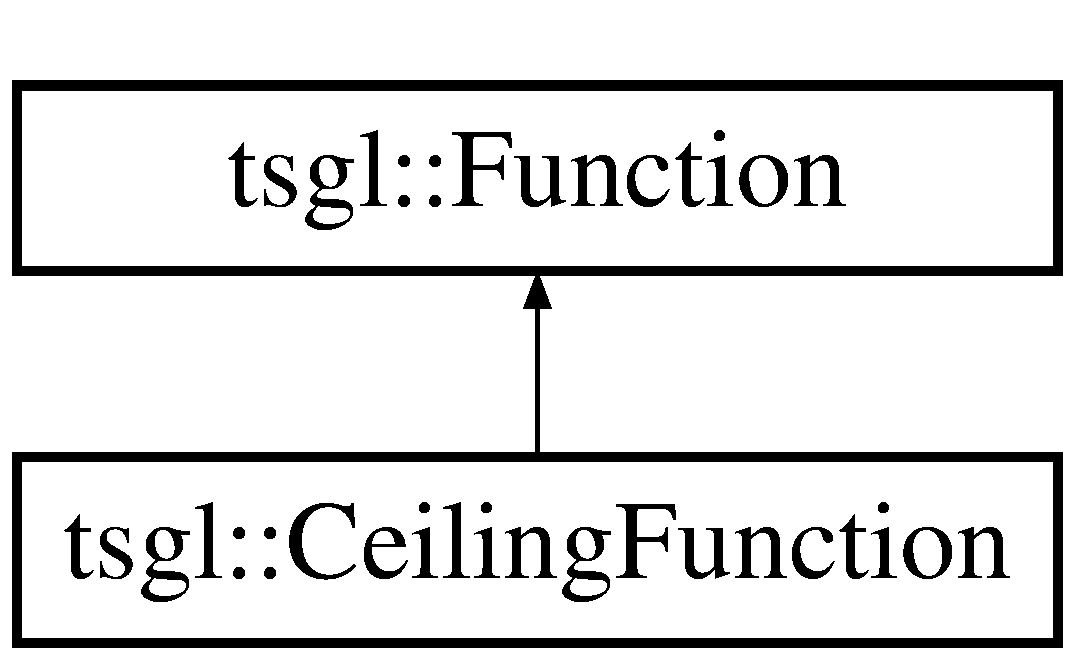
\includegraphics[height=2.000000cm]{classtsgl_1_1_ceiling_function}
\end{center}
\end{figure}
\subsection*{Public Member Functions}
\begin{DoxyCompactItemize}
\item 
virtual Decimal \hyperlink{classtsgl_1_1_ceiling_function_ab47498860b2395e331f203c4025bcb81}{value\+At} (Decimal x) const 
\begin{DoxyCompactList}\small\item\em Method to determine the value of \hyperlink{classtsgl_1_1_ceiling_function}{Ceiling\+Function}. \end{DoxyCompactList}\end{DoxyCompactItemize}


\subsection{Detailed Description}
\hyperlink{classtsgl_1_1_function}{Function} to compute the mathematical ceiling of the input. 

\subsection{Member Function Documentation}
\hypertarget{classtsgl_1_1_ceiling_function_ab47498860b2395e331f203c4025bcb81}{}\index{tsgl\+::\+Ceiling\+Function@{tsgl\+::\+Ceiling\+Function}!value\+At@{value\+At}}
\index{value\+At@{value\+At}!tsgl\+::\+Ceiling\+Function@{tsgl\+::\+Ceiling\+Function}}
\subsubsection[{value\+At}]{\setlength{\rightskip}{0pt plus 5cm}virtual Decimal tsgl\+::\+Ceiling\+Function\+::value\+At (
\begin{DoxyParamCaption}
\item[{Decimal}]{x}
\end{DoxyParamCaption}
) const\hspace{0.3cm}{\ttfamily [inline]}, {\ttfamily [virtual]}}\label{classtsgl_1_1_ceiling_function_ab47498860b2395e331f203c4025bcb81}


Method to determine the value of \hyperlink{classtsgl_1_1_ceiling_function}{Ceiling\+Function}. 

\begin{DoxyReturn}{Returns}
The smallest integer greater than or equal to {\itshape x}. 
\end{DoxyReturn}


Implements \hyperlink{classtsgl_1_1_function_affb7b3b19a04efefa29a9870d666e912}{tsgl\+::\+Function}.



The documentation for this class was generated from the following file\+:\begin{DoxyCompactItemize}
\item 
Function.\+h\end{DoxyCompactItemize}

\hypertarget{classtsgl_1_1_circle}{}\section{tsgl\+:\+:Circle Class Reference}
\label{classtsgl_1_1_circle}\index{tsgl\+::\+Circle@{tsgl\+::\+Circle}}


Draw a circle.  




{\ttfamily \#include $<$Circle.\+h$>$}

Inheritance diagram for tsgl\+:\+:Circle\+:\begin{figure}[H]
\begin{center}
\leavevmode
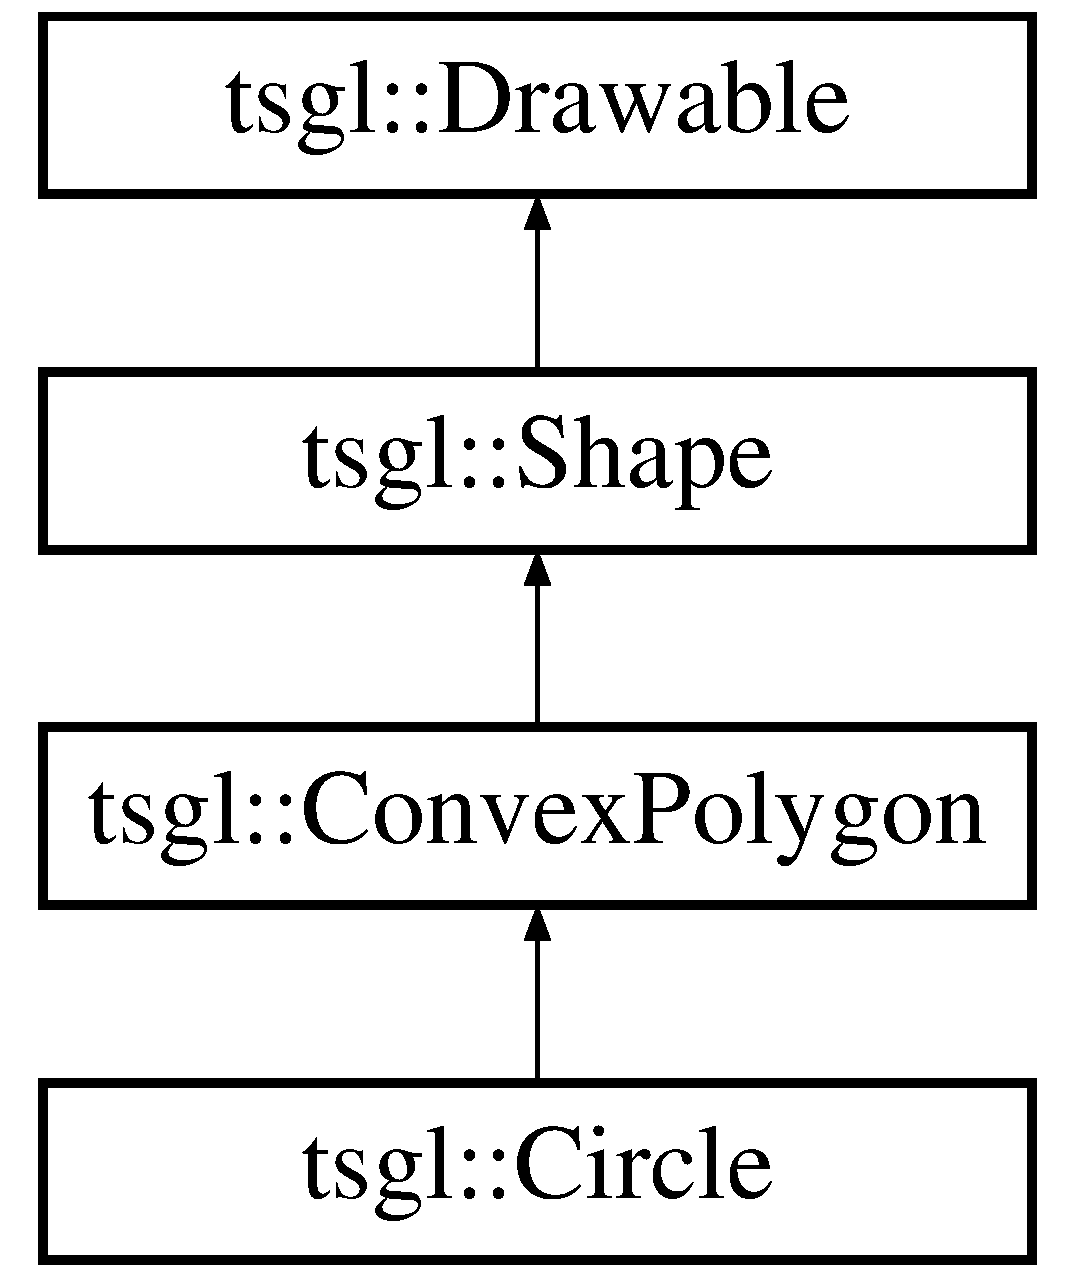
\includegraphics[height=4.000000cm]{classtsgl_1_1_circle}
\end{center}
\end{figure}
\subsection*{Public Member Functions}
\begin{DoxyCompactItemize}
\item 
\hyperlink{classtsgl_1_1_circle_aed06fe2620b6fc81ecc3d6ed94e47aeb}{Circle} (float x, float y, float z, G\+Lfloat radius, float yaw, float pitch, float roll, \hyperlink{structtsgl_1_1_color_float}{Color\+Float} color)
\begin{DoxyCompactList}\small\item\em Explicitly constructs a new monocolored filled \hyperlink{classtsgl_1_1_circle}{Circle}. \end{DoxyCompactList}\item 
\hyperlink{classtsgl_1_1_circle_aeee2a7388c304fd8deb601d426dc0211}{Circle} (float x, float y, float z, G\+Lfloat radius, float yaw, float pitch, float roll, \hyperlink{structtsgl_1_1_color_float}{Color\+Float} color\mbox{[}$\,$\mbox{]})
\begin{DoxyCompactList}\small\item\em Explicitly constructs a new multicolored filled \hyperlink{classtsgl_1_1_circle}{Circle}. \end{DoxyCompactList}\item 
void \hyperlink{classtsgl_1_1_circle_a515710a6bbec274a1b8686c0d427a0d5}{set\+Radius} (G\+Lfloat radius)
\begin{DoxyCompactList}\small\item\em Mutates the radius of the \hyperlink{classtsgl_1_1_circle}{Circle}. \end{DoxyCompactList}\item 
void \hyperlink{classtsgl_1_1_circle_a1778df77ca0903a9a4d3060b10ff7925}{change\+Radius\+By} (G\+Lfloat delta)
\begin{DoxyCompactList}\small\item\em Mutates the radius of the \hyperlink{classtsgl_1_1_circle}{Circle} by the parameter amount. \end{DoxyCompactList}\item 
G\+Lfloat \hyperlink{classtsgl_1_1_circle_ab6b2d16691b472d04972b1860856e7dd}{get\+Radius} ()
\begin{DoxyCompactList}\small\item\em Accessor for the radius of the \hyperlink{classtsgl_1_1_circle}{Circle}. \end{DoxyCompactList}\item 
void \hyperlink{classtsgl_1_1_circle_a3e97ff653a534a606f0a3b3176c330b0}{set\+Color} (\hyperlink{structtsgl_1_1_color_float}{Color\+Float} c)
\begin{DoxyCompactList}\small\item\em Sets the \hyperlink{classtsgl_1_1_shape}{Shape} to a new color. \end{DoxyCompactList}\item 
void \hyperlink{classtsgl_1_1_circle_aa25c336d07fb8216bd5d6f63f53a2271}{set\+Color} (\hyperlink{structtsgl_1_1_color_float}{Color\+Float} c\mbox{[}$\,$\mbox{]})
\begin{DoxyCompactList}\small\item\em Sets the \hyperlink{classtsgl_1_1_circle}{Circle} to a new array of colors. \end{DoxyCompactList}\item 
virtual void \hyperlink{classtsgl_1_1_circle_af0e1ef7313bde5f66750b616de296f76}{get\+Colors} (std\+::vector$<$ \hyperlink{structtsgl_1_1_color_float}{Color\+Float} $>$ \&color\+Vec)
\begin{DoxyCompactList}\small\item\em Accessor for \hyperlink{classtsgl_1_1_circle}{Circle}\textquotesingle{}s colors. \end{DoxyCompactList}\end{DoxyCompactItemize}
\subsection*{Protected Attributes}
\begin{DoxyCompactItemize}
\item 
\mbox{\Hypertarget{classtsgl_1_1_circle_a60107a7f25bc0216daf628e24264a7a5}\label{classtsgl_1_1_circle_a60107a7f25bc0216daf628e24264a7a5}} 
G\+Lfloat {\bfseries my\+Radius}
\item 
\mbox{\Hypertarget{classtsgl_1_1_circle_a513d9c5e6e8b7b32c2e10756835a1612}\label{classtsgl_1_1_circle_a513d9c5e6e8b7b32c2e10756835a1612}} 
G\+Lfloat {\bfseries vertices\+Per\+Color}
\end{DoxyCompactItemize}
\subsection*{Additional Inherited Members}


\subsection{Detailed Description}
Draw a circle. 

\hyperlink{classtsgl_1_1_circle}{Circle} is a class for holding \hyperlink{classtsgl_1_1_shape}{Shape} data for a circle. 

\subsection{Constructor \& Destructor Documentation}
\mbox{\Hypertarget{classtsgl_1_1_circle_aed06fe2620b6fc81ecc3d6ed94e47aeb}\label{classtsgl_1_1_circle_aed06fe2620b6fc81ecc3d6ed94e47aeb}} 
\index{tsgl\+::\+Circle@{tsgl\+::\+Circle}!Circle@{Circle}}
\index{Circle@{Circle}!tsgl\+::\+Circle@{tsgl\+::\+Circle}}
\subsubsection{\texorpdfstring{Circle()}{Circle()}\hspace{0.1cm}{\footnotesize\ttfamily [1/2]}}
{\footnotesize\ttfamily tsgl\+::\+Circle\+::\+Circle (\begin{DoxyParamCaption}\item[{float}]{x,  }\item[{float}]{y,  }\item[{float}]{z,  }\item[{G\+Lfloat}]{radius,  }\item[{float}]{yaw,  }\item[{float}]{pitch,  }\item[{float}]{roll,  }\item[{\hyperlink{structtsgl_1_1_color_float}{Color\+Float}}]{color }\end{DoxyParamCaption})}



Explicitly constructs a new monocolored filled \hyperlink{classtsgl_1_1_circle}{Circle}. 

This function draws a circle with the given center, radius, 3D rotation, color. 
\begin{DoxyParams}{Parameters}
{\em x} & The x coordinate of the circle\textquotesingle{}s center. \\
\hline
{\em y} & The y coordinate of the circle\textquotesingle{}s center. \\
\hline
{\em z} & The z coordinate of the circle\textquotesingle{}s center. \\
\hline
{\em radius} & The radius of the circle in pixels. \\
\hline
{\em yaw} & The circle\textquotesingle{}s yaw in 3D space. \\
\hline
{\em pitch} & The circle\textquotesingle{}s pitch in 3D space. \\
\hline
{\em roll} & The circle\textquotesingle{}s roll in 3D space. \\
\hline
{\em color} & The color of the circle\textquotesingle{}s fill \\
\hline
\end{DoxyParams}
\mbox{\Hypertarget{classtsgl_1_1_circle_aeee2a7388c304fd8deb601d426dc0211}\label{classtsgl_1_1_circle_aeee2a7388c304fd8deb601d426dc0211}} 
\index{tsgl\+::\+Circle@{tsgl\+::\+Circle}!Circle@{Circle}}
\index{Circle@{Circle}!tsgl\+::\+Circle@{tsgl\+::\+Circle}}
\subsubsection{\texorpdfstring{Circle()}{Circle()}\hspace{0.1cm}{\footnotesize\ttfamily [2/2]}}
{\footnotesize\ttfamily tsgl\+::\+Circle\+::\+Circle (\begin{DoxyParamCaption}\item[{float}]{x,  }\item[{float}]{y,  }\item[{float}]{z,  }\item[{G\+Lfloat}]{radius,  }\item[{float}]{yaw,  }\item[{float}]{pitch,  }\item[{float}]{roll,  }\item[{\hyperlink{structtsgl_1_1_color_float}{Color\+Float}}]{color\mbox{[}$\,$\mbox{]} }\end{DoxyParamCaption})}



Explicitly constructs a new multicolored filled \hyperlink{classtsgl_1_1_circle}{Circle}. 

This function draws a circle with the given center, radius, roation, and fill color. 
\begin{DoxyParams}{Parameters}
{\em x} & The x coordinate of the circle\textquotesingle{}s center. \\
\hline
{\em y} & The y coordinate of the circle\textquotesingle{}s center. \\
\hline
{\em z} & The z coordinate of the circle\textquotesingle{}s center. \\
\hline
{\em radius} & The radius of the circle in pixels. \\
\hline
{\em yaw} & The circle\textquotesingle{}s yaw in 3D space. \\
\hline
{\em pitch} & The circle\textquotesingle{}s pitch in 3D space. \\
\hline
{\em roll} & The circle\textquotesingle{}s roll in 3D space. \\
\hline
{\em color} & An array of colors for the \hyperlink{classtsgl_1_1_circle}{Circle}\textquotesingle{}s fill \\
\hline
\end{DoxyParams}


\subsection{Member Function Documentation}
\mbox{\Hypertarget{classtsgl_1_1_circle_a1778df77ca0903a9a4d3060b10ff7925}\label{classtsgl_1_1_circle_a1778df77ca0903a9a4d3060b10ff7925}} 
\index{tsgl\+::\+Circle@{tsgl\+::\+Circle}!change\+Radius\+By@{change\+Radius\+By}}
\index{change\+Radius\+By@{change\+Radius\+By}!tsgl\+::\+Circle@{tsgl\+::\+Circle}}
\subsubsection{\texorpdfstring{change\+Radius\+By()}{changeRadiusBy()}}
{\footnotesize\ttfamily void tsgl\+::\+Circle\+::change\+Radius\+By (\begin{DoxyParamCaption}\item[{G\+Lfloat}]{delta }\end{DoxyParamCaption})}



Mutates the radius of the \hyperlink{classtsgl_1_1_circle}{Circle} by the parameter amount. 


\begin{DoxyParams}{Parameters}
{\em delta} & The amount by which to change the radius of the \hyperlink{classtsgl_1_1_circle}{Circle}. \\
\hline
\end{DoxyParams}
\mbox{\Hypertarget{classtsgl_1_1_circle_af0e1ef7313bde5f66750b616de296f76}\label{classtsgl_1_1_circle_af0e1ef7313bde5f66750b616de296f76}} 
\index{tsgl\+::\+Circle@{tsgl\+::\+Circle}!get\+Colors@{get\+Colors}}
\index{get\+Colors@{get\+Colors}!tsgl\+::\+Circle@{tsgl\+::\+Circle}}
\subsubsection{\texorpdfstring{get\+Colors()}{getColors()}}
{\footnotesize\ttfamily void tsgl\+::\+Circle\+::get\+Colors (\begin{DoxyParamCaption}\item[{std\+::vector$<$ \hyperlink{structtsgl_1_1_color_float}{Color\+Float} $>$ \&}]{color\+Vec }\end{DoxyParamCaption})\hspace{0.3cm}{\ttfamily [virtual]}}



Accessor for \hyperlink{classtsgl_1_1_circle}{Circle}\textquotesingle{}s colors. 

Populates the reference parameter vector with a \hyperlink{structtsgl_1_1_color_float}{Color\+Float} for each section of \hyperlink{classtsgl_1_1_circle}{Circle}. 
\begin{DoxyParams}{Parameters}
{\em color\+Vec} & A vector of Color\+Floats to which the Color\+Floats associated with \hyperlink{classtsgl_1_1_circle}{Circle} will be pushed. \\
\hline
\end{DoxyParams}
\begin{DoxyNote}{Note}
Overrides \hyperlink{classtsgl_1_1_shape_a6f54fe4d049f69a287edf8335a9509f8}{Shape\+::get\+Colors()}. 
\end{DoxyNote}


Reimplemented from \hyperlink{classtsgl_1_1_shape_a6f54fe4d049f69a287edf8335a9509f8}{tsgl\+::\+Shape}.



Referenced by set\+Color().

\mbox{\Hypertarget{classtsgl_1_1_circle_ab6b2d16691b472d04972b1860856e7dd}\label{classtsgl_1_1_circle_ab6b2d16691b472d04972b1860856e7dd}} 
\index{tsgl\+::\+Circle@{tsgl\+::\+Circle}!get\+Radius@{get\+Radius}}
\index{get\+Radius@{get\+Radius}!tsgl\+::\+Circle@{tsgl\+::\+Circle}}
\subsubsection{\texorpdfstring{get\+Radius()}{getRadius()}}
{\footnotesize\ttfamily G\+Lfloat tsgl\+::\+Circle\+::get\+Radius (\begin{DoxyParamCaption}{ }\end{DoxyParamCaption})\hspace{0.3cm}{\ttfamily [inline]}}



Accessor for the radius of the \hyperlink{classtsgl_1_1_circle}{Circle}. 

Returns the value of the my\+Radius private variable, a G\+Lfloat. \mbox{\Hypertarget{classtsgl_1_1_circle_a3e97ff653a534a606f0a3b3176c330b0}\label{classtsgl_1_1_circle_a3e97ff653a534a606f0a3b3176c330b0}} 
\index{tsgl\+::\+Circle@{tsgl\+::\+Circle}!set\+Color@{set\+Color}}
\index{set\+Color@{set\+Color}!tsgl\+::\+Circle@{tsgl\+::\+Circle}}
\subsubsection{\texorpdfstring{set\+Color()}{setColor()}\hspace{0.1cm}{\footnotesize\ttfamily [1/2]}}
{\footnotesize\ttfamily void tsgl\+::\+Circle\+::set\+Color (\begin{DoxyParamCaption}\item[{\hyperlink{structtsgl_1_1_color_float}{Color\+Float}}]{c }\end{DoxyParamCaption})\hspace{0.3cm}{\ttfamily [inline]}, {\ttfamily [virtual]}}



Sets the \hyperlink{classtsgl_1_1_shape}{Shape} to a new color. 


\begin{DoxyParams}{Parameters}
{\em c} & The new \hyperlink{structtsgl_1_1_color_float}{Color\+Float}. \\
\hline
\end{DoxyParams}


Reimplemented from \hyperlink{classtsgl_1_1_shape_abdb01321cddfd2db1481eefbc2836f70}{tsgl\+::\+Shape}.



Referenced by Reader\+::\+Reader(), Philosopher\+::refresh\+Color(), and Writer\+::\+Writer().

\mbox{\Hypertarget{classtsgl_1_1_circle_aa25c336d07fb8216bd5d6f63f53a2271}\label{classtsgl_1_1_circle_aa25c336d07fb8216bd5d6f63f53a2271}} 
\index{tsgl\+::\+Circle@{tsgl\+::\+Circle}!set\+Color@{set\+Color}}
\index{set\+Color@{set\+Color}!tsgl\+::\+Circle@{tsgl\+::\+Circle}}
\subsubsection{\texorpdfstring{set\+Color()}{setColor()}\hspace{0.1cm}{\footnotesize\ttfamily [2/2]}}
{\footnotesize\ttfamily void tsgl\+::\+Circle\+::set\+Color (\begin{DoxyParamCaption}\item[{\hyperlink{structtsgl_1_1_color_float}{Color\+Float}}]{c\mbox{[}$\,$\mbox{]} }\end{DoxyParamCaption})\hspace{0.3cm}{\ttfamily [virtual]}}



Sets the \hyperlink{classtsgl_1_1_circle}{Circle} to a new array of colors. 


\begin{DoxyParams}{Parameters}
{\em c} & An array of the new Color\+Floats. \\
\hline
\end{DoxyParams}


Reimplemented from \hyperlink{classtsgl_1_1_shape_ad7e554b5d4cea111ec518548b9f21388}{tsgl\+::\+Shape}.

\mbox{\Hypertarget{classtsgl_1_1_circle_a515710a6bbec274a1b8686c0d427a0d5}\label{classtsgl_1_1_circle_a515710a6bbec274a1b8686c0d427a0d5}} 
\index{tsgl\+::\+Circle@{tsgl\+::\+Circle}!set\+Radius@{set\+Radius}}
\index{set\+Radius@{set\+Radius}!tsgl\+::\+Circle@{tsgl\+::\+Circle}}
\subsubsection{\texorpdfstring{set\+Radius()}{setRadius()}}
{\footnotesize\ttfamily void tsgl\+::\+Circle\+::set\+Radius (\begin{DoxyParamCaption}\item[{G\+Lfloat}]{radius }\end{DoxyParamCaption})}



Mutates the radius of the \hyperlink{classtsgl_1_1_circle}{Circle}. 


\begin{DoxyParams}{Parameters}
{\em radius} & The \hyperlink{classtsgl_1_1_circle}{Circle}\textquotesingle{}s new radius. \\
\hline
\end{DoxyParams}


The documentation for this class was generated from the following files\+:\begin{DoxyCompactItemize}
\item 
Circle.\+h\item 
Circle.\+cpp\end{DoxyCompactItemize}

\hypertarget{structtsgl_1_1_color_float}{}\section{tsgl\+:\+:Color\+Float Struct Reference}
\label{structtsgl_1_1_color_float}\index{tsgl\+::\+Color\+Float@{tsgl\+::\+Color\+Float}}


Floating point R\+G\+B\+A color struct.  




{\ttfamily \#include $<$Color.\+h$>$}

\subsection*{Public Member Functions}
\begin{DoxyCompactItemize}
\item 
\hyperlink{structtsgl_1_1_color_float_a22e82c71a0feedbb7b3e3a7a73b80e30}{Color\+Float} ()
\begin{DoxyCompactList}\small\item\em Default \hyperlink{structtsgl_1_1_color_float}{Color\+Float} constructor method. \end{DoxyCompactList}\item 
\hyperlink{structtsgl_1_1_color_float_a134643b43f1d8acaed32095f04942140}{Color\+Float} (float v, float a=1.\+0f)
\begin{DoxyCompactList}\small\item\em Basic explicit \hyperlink{structtsgl_1_1_color_float}{Color\+Float} constructor method. \end{DoxyCompactList}\item 
\hyperlink{structtsgl_1_1_color_float_a6c46a2073d9e208aa3f07cc04565a489}{Color\+Float} (float r, float g, float b, float a=1.\+0f)
\begin{DoxyCompactList}\small\item\em Full explicit \hyperlink{structtsgl_1_1_color_float}{Color\+Float} constructor method. \end{DoxyCompactList}\item 
std\+::string \hyperlink{structtsgl_1_1_color_float_a1048e8773d65fa1554bc8782e76527ed}{as\+String} ()
\begin{DoxyCompactList}\small\item\em Returns a string representation of the \hyperlink{structtsgl_1_1_color_float}{Color\+Float}. \end{DoxyCompactList}\item 
\hyperlink{structtsgl_1_1_color_float_a4d74b061239eed7eb351422c18e33a37}{operator Color\+H\+S\+V} ()
\begin{DoxyCompactList}\small\item\em Implicit conversion from \hyperlink{structtsgl_1_1_color_float}{Color\+Float} to \hyperlink{structtsgl_1_1_color_h_s_v}{Color\+H\+S\+V}. \end{DoxyCompactList}\item 
\hyperlink{structtsgl_1_1_color_float_a4ef5398fd1ee469dd9b1b43c9ce5c00d}{operator Color\+Int} ()
\begin{DoxyCompactList}\small\item\em Implicit conversion from \hyperlink{structtsgl_1_1_color_float}{Color\+Float} to \hyperlink{structtsgl_1_1_color_int}{Color\+Int}. \end{DoxyCompactList}\item 
\hyperlink{structtsgl_1_1_color_float}{Color\+Float} \hyperlink{structtsgl_1_1_color_float_a09d7cc47ac3d0e23ef7339ccf33111a5}{operator$\ast$} (float f)
\begin{DoxyCompactList}\small\item\em Multiplies the values of a \hyperlink{structtsgl_1_1_color_float}{Color\+Float} by a float. \end{DoxyCompactList}\item 
bool \hyperlink{structtsgl_1_1_color_float_ac29ecf4a36624050af433d691e65651c}{operator==} (\hyperlink{structtsgl_1_1_color_float}{Color\+Float} \&c2)
\begin{DoxyCompactList}\small\item\em Determines if two Color\+Floats are equivalent. \end{DoxyCompactList}\item 
bool \hyperlink{structtsgl_1_1_color_float_afd92fcf8743d931cfbcf405209c923fc}{operator!=} (\hyperlink{structtsgl_1_1_color_float}{Color\+Float} \&c2)
\begin{DoxyCompactList}\small\item\em Determines if two Color\+Floats are {\itshape N\+O\+T} equivalent. \end{DoxyCompactList}\end{DoxyCompactItemize}
\subsection*{Public Attributes}
\begin{DoxyCompactItemize}
\item 
\hypertarget{structtsgl_1_1_color_float_a15c36dbebaccfc982b0b07af95214d10}{}float {\bfseries R}\label{structtsgl_1_1_color_float_a15c36dbebaccfc982b0b07af95214d10}

\item 
\hypertarget{structtsgl_1_1_color_float_a7a7f1659d2f7694625f4a393a57686b4}{}float {\bfseries G}\label{structtsgl_1_1_color_float_a7a7f1659d2f7694625f4a393a57686b4}

\item 
\hypertarget{structtsgl_1_1_color_float_ae0c874ce1bc4a3fb725bbae35411a794}{}float {\bfseries B}\label{structtsgl_1_1_color_float_ae0c874ce1bc4a3fb725bbae35411a794}

\item 
\hypertarget{structtsgl_1_1_color_float_aba05ee650a72ae8e3c4683b54bf192fb}{}float {\bfseries A}\label{structtsgl_1_1_color_float_aba05ee650a72ae8e3c4683b54bf192fb}

\end{DoxyCompactItemize}


\subsection{Detailed Description}
Floating point R\+G\+B\+A color struct. 

\hyperlink{structtsgl_1_1_color_float}{Color\+Float} defines a color with floating point red, green, blue, and alpha components. 
\begin{DoxyParams}{Parameters}
{\em R} & Red component, between 0 and 1 inclusive. \\
\hline
{\em G} & Green component, between 0 and 1 inclusive. \\
\hline
{\em B} & Blue component, between 0 and 1 inclusive. \\
\hline
{\em A} & Alpha component, between 0 and 1 inclusive. \\
\hline
\end{DoxyParams}


\subsection{Constructor \& Destructor Documentation}
\hypertarget{structtsgl_1_1_color_float_a22e82c71a0feedbb7b3e3a7a73b80e30}{}\index{tsgl\+::\+Color\+Float@{tsgl\+::\+Color\+Float}!Color\+Float@{Color\+Float}}
\index{Color\+Float@{Color\+Float}!tsgl\+::\+Color\+Float@{tsgl\+::\+Color\+Float}}
\subsubsection[{Color\+Float}]{\setlength{\rightskip}{0pt plus 5cm}tsgl\+::\+Color\+Float\+::\+Color\+Float (
\begin{DoxyParamCaption}
{}
\end{DoxyParamCaption}
)}\label{structtsgl_1_1_color_float_a22e82c71a0feedbb7b3e3a7a73b80e30}


Default \hyperlink{structtsgl_1_1_color_float}{Color\+Float} constructor method. 

This is the default constructor for the \hyperlink{structtsgl_1_1_color_float}{Color\+Float} struct. \begin{DoxyNote}{Note}
R, G, B, and A are all set to 1.\+0f by default. 
\end{DoxyNote}
\begin{DoxyReturn}{Returns}
A \hyperlink{structtsgl_1_1_color_float}{Color\+Float} struct with default R, G, B, and A values. 
\end{DoxyReturn}


Referenced by operator$\ast$().

\hypertarget{structtsgl_1_1_color_float_a134643b43f1d8acaed32095f04942140}{}\index{tsgl\+::\+Color\+Float@{tsgl\+::\+Color\+Float}!Color\+Float@{Color\+Float}}
\index{Color\+Float@{Color\+Float}!tsgl\+::\+Color\+Float@{tsgl\+::\+Color\+Float}}
\subsubsection[{Color\+Float}]{\setlength{\rightskip}{0pt plus 5cm}tsgl\+::\+Color\+Float\+::\+Color\+Float (
\begin{DoxyParamCaption}
\item[{float}]{v, }
\item[{float}]{a = {\ttfamily 1.0f}}
\end{DoxyParamCaption}
)}\label{structtsgl_1_1_color_float_a134643b43f1d8acaed32095f04942140}


Basic explicit \hyperlink{structtsgl_1_1_color_float}{Color\+Float} constructor method. 

This is the basic explicit constructor for the \hyperlink{structtsgl_1_1_color_float}{Color\+Float} struct. 
\begin{DoxyParams}{Parameters}
{\em v} & The value component of the color. \\
\hline
{\em a} & The alpha component of the struct (set to 1.\+0f by default). \\
\hline
\end{DoxyParams}
\begin{DoxyWarning}{Warning}
An invariant is set where if any of the specified R, G, B, or A values is out of the range 0 -\/ 1 inclusive then an error message is given. 
\end{DoxyWarning}
\begin{DoxyReturn}{Returns}
A \hyperlink{structtsgl_1_1_color_float}{Color\+Float} struct with equal R, G, and B values set to {\ttfamily v}, and the specified A value. 
\end{DoxyReturn}
\hypertarget{structtsgl_1_1_color_float_a6c46a2073d9e208aa3f07cc04565a489}{}\index{tsgl\+::\+Color\+Float@{tsgl\+::\+Color\+Float}!Color\+Float@{Color\+Float}}
\index{Color\+Float@{Color\+Float}!tsgl\+::\+Color\+Float@{tsgl\+::\+Color\+Float}}
\subsubsection[{Color\+Float}]{\setlength{\rightskip}{0pt plus 5cm}tsgl\+::\+Color\+Float\+::\+Color\+Float (
\begin{DoxyParamCaption}
\item[{float}]{r, }
\item[{float}]{g, }
\item[{float}]{b, }
\item[{float}]{a = {\ttfamily 1.0f}}
\end{DoxyParamCaption}
)}\label{structtsgl_1_1_color_float_a6c46a2073d9e208aa3f07cc04565a489}


Full explicit \hyperlink{structtsgl_1_1_color_float}{Color\+Float} constructor method. 

This is the full explicit constructor for the \hyperlink{structtsgl_1_1_color_float}{Color\+Float} struct. 
\begin{DoxyParams}{Parameters}
{\em r} & The red component of the struct. \\
\hline
{\em g} & The green component of the struct. \\
\hline
{\em b} & The blue component of the struct. \\
\hline
{\em a} & The alpha component of the struct (set to 1.\+0f by default). \\
\hline
\end{DoxyParams}
\begin{DoxyWarning}{Warning}
An invariant is set where if any of the specified R, G, B, or A values is out of the range 0 -\/ 1 inclusive then an error message is given. 
\end{DoxyWarning}
\begin{DoxyReturn}{Returns}
A \hyperlink{structtsgl_1_1_color_float}{Color\+Float} struct with the specified R, G, B, and A values. 
\end{DoxyReturn}


\subsection{Member Function Documentation}
\hypertarget{structtsgl_1_1_color_float_a1048e8773d65fa1554bc8782e76527ed}{}\index{tsgl\+::\+Color\+Float@{tsgl\+::\+Color\+Float}!as\+String@{as\+String}}
\index{as\+String@{as\+String}!tsgl\+::\+Color\+Float@{tsgl\+::\+Color\+Float}}
\subsubsection[{as\+String}]{\setlength{\rightskip}{0pt plus 5cm}std\+::string tsgl\+::\+Color\+Float\+::as\+String (
\begin{DoxyParamCaption}
{}
\end{DoxyParamCaption}
)}\label{structtsgl_1_1_color_float_a1048e8773d65fa1554bc8782e76527ed}


Returns a string representation of the \hyperlink{structtsgl_1_1_color_float}{Color\+Float}. 

This function returns a std\+::string representation of the \hyperlink{structtsgl_1_1_color_float}{Color\+Float}. \begin{DoxyReturn}{Returns}
A string representation of the \hyperlink{structtsgl_1_1_color_float}{Color\+Float}. 
\end{DoxyReturn}
\hypertarget{structtsgl_1_1_color_float_a4d74b061239eed7eb351422c18e33a37}{}\index{tsgl\+::\+Color\+Float@{tsgl\+::\+Color\+Float}!operator Color\+H\+S\+V@{operator Color\+H\+S\+V}}
\index{operator Color\+H\+S\+V@{operator Color\+H\+S\+V}!tsgl\+::\+Color\+Float@{tsgl\+::\+Color\+Float}}
\subsubsection[{operator Color\+H\+S\+V}]{\setlength{\rightskip}{0pt plus 5cm}tsgl\+::\+Color\+Float\+::operator {\bf Color\+H\+S\+V} (
\begin{DoxyParamCaption}
{}
\end{DoxyParamCaption}
)}\label{structtsgl_1_1_color_float_a4d74b061239eed7eb351422c18e33a37}


Implicit conversion from \hyperlink{structtsgl_1_1_color_float}{Color\+Float} to \hyperlink{structtsgl_1_1_color_h_s_v}{Color\+H\+S\+V}. 

This defines the implicit conversion operator from a floating point color type (\hyperlink{structtsgl_1_1_color_float}{Color\+Float}) to an H\+S\+V color type (\hyperlink{structtsgl_1_1_color_h_s_v}{Color\+H\+S\+V}). \hypertarget{structtsgl_1_1_color_float_a4ef5398fd1ee469dd9b1b43c9ce5c00d}{}\index{tsgl\+::\+Color\+Float@{tsgl\+::\+Color\+Float}!operator Color\+Int@{operator Color\+Int}}
\index{operator Color\+Int@{operator Color\+Int}!tsgl\+::\+Color\+Float@{tsgl\+::\+Color\+Float}}
\subsubsection[{operator Color\+Int}]{\setlength{\rightskip}{0pt plus 5cm}tsgl\+::\+Color\+Float\+::operator {\bf Color\+Int} (
\begin{DoxyParamCaption}
{}
\end{DoxyParamCaption}
)}\label{structtsgl_1_1_color_float_a4ef5398fd1ee469dd9b1b43c9ce5c00d}


Implicit conversion from \hyperlink{structtsgl_1_1_color_float}{Color\+Float} to \hyperlink{structtsgl_1_1_color_int}{Color\+Int}. 

This defines the implicit conversion operator from a floating point color type (\hyperlink{structtsgl_1_1_color_float}{Color\+Float}) to an integer color type (\hyperlink{structtsgl_1_1_color_int}{Color\+Int}). \hypertarget{structtsgl_1_1_color_float_afd92fcf8743d931cfbcf405209c923fc}{}\index{tsgl\+::\+Color\+Float@{tsgl\+::\+Color\+Float}!operator"!=@{operator"!=}}
\index{operator"!=@{operator"!=}!tsgl\+::\+Color\+Float@{tsgl\+::\+Color\+Float}}
\subsubsection[{operator"!=}]{\setlength{\rightskip}{0pt plus 5cm}bool tsgl\+::\+Color\+Float\+::operator!= (
\begin{DoxyParamCaption}
\item[{{\bf Color\+Float} \&}]{c2}
\end{DoxyParamCaption}
)}\label{structtsgl_1_1_color_float_afd92fcf8743d931cfbcf405209c923fc}


Determines if two Color\+Floats are {\itshape N\+O\+T} equivalent. 

Inequality operator for two Color\+Floats. Determines if they are {\itshape N\+O\+T} equivalent. 
\begin{DoxyParams}{Parameters}
{\em c2} & Reference to the \hyperlink{structtsgl_1_1_color_float}{Color\+Float} struct that is the second one in the inequality comparison. \\
\hline
\end{DoxyParams}
\begin{DoxyNote}{Note}
This function relies on ($\ast$this), which is a dereferenced pointer to the first \hyperlink{structtsgl_1_1_color_float}{Color\+Float} struct in the inequality comparison. (its the one on the left side of the != sign). 
\end{DoxyNote}
\begin{DoxyReturn}{Returns}
true if the two Color\+Floats are not equivalent, false if otherwise. 
\end{DoxyReturn}
\hypertarget{structtsgl_1_1_color_float_a09d7cc47ac3d0e23ef7339ccf33111a5}{}\index{tsgl\+::\+Color\+Float@{tsgl\+::\+Color\+Float}!operator$\ast$@{operator$\ast$}}
\index{operator$\ast$@{operator$\ast$}!tsgl\+::\+Color\+Float@{tsgl\+::\+Color\+Float}}
\subsubsection[{operator$\ast$}]{\setlength{\rightskip}{0pt plus 5cm}{\bf Color\+Float} tsgl\+::\+Color\+Float\+::operator$\ast$ (
\begin{DoxyParamCaption}
\item[{float}]{f}
\end{DoxyParamCaption}
)}\label{structtsgl_1_1_color_float_a09d7cc47ac3d0e23ef7339ccf33111a5}


Multiplies the values of a \hyperlink{structtsgl_1_1_color_float}{Color\+Float} by a float. 

This operator multiplies each of the components of a \hyperlink{structtsgl_1_1_color_float}{Color\+Float} by amount {\ttfamily f}. 
\begin{DoxyParams}{Parameters}
{\em f} & Amount to multiply each component by \\
\hline
\end{DoxyParams}
\begin{DoxyReturn}{Returns}
A new \hyperlink{structtsgl_1_1_color_float}{Color\+Float} constructed as \hyperlink{structtsgl_1_1_color_float}{Color\+Float}(orig.\+R$\ast$f, orig.\+G$\ast$f, orig.\+b$\ast$f, orig.\+A$\ast$f) 
\end{DoxyReturn}
\begin{DoxyNote}{Note}
Individual channels are clamped between 0 and 1. 
\end{DoxyNote}
\hypertarget{structtsgl_1_1_color_float_ac29ecf4a36624050af433d691e65651c}{}\index{tsgl\+::\+Color\+Float@{tsgl\+::\+Color\+Float}!operator==@{operator==}}
\index{operator==@{operator==}!tsgl\+::\+Color\+Float@{tsgl\+::\+Color\+Float}}
\subsubsection[{operator==}]{\setlength{\rightskip}{0pt plus 5cm}bool tsgl\+::\+Color\+Float\+::operator== (
\begin{DoxyParamCaption}
\item[{{\bf Color\+Float} \&}]{c2}
\end{DoxyParamCaption}
)}\label{structtsgl_1_1_color_float_ac29ecf4a36624050af433d691e65651c}


Determines if two Color\+Floats are equivalent. 

Equality operator for two Color\+Floats. Determines if they are equivalent. 
\begin{DoxyParams}{Parameters}
{\em c2} & Reference to the \hyperlink{structtsgl_1_1_color_float}{Color\+Float} struct that is the second one in the equivalence comparison. \\
\hline
\end{DoxyParams}
\begin{DoxyNote}{Note}
This function relies on ($\ast$this), which is a dereferenced pointer to the first \hyperlink{structtsgl_1_1_color_float}{Color\+Float} struct in the comparison. (its the one on the left side of the == sign). 
\end{DoxyNote}
\begin{DoxyReturn}{Returns}
true if the two Color\+Floats are equivalent, false if otherwise. 
\end{DoxyReturn}


The documentation for this struct was generated from the following files\+:\begin{DoxyCompactItemize}
\item 
Color.\+h\item 
Color.\+cpp\end{DoxyCompactItemize}

\hypertarget{structtsgl_1_1_color_h_s_v}{}\section{tsgl\+:\+:Color\+H\+S\+V Struct Reference}
\label{structtsgl_1_1_color_h_s_v}\index{tsgl\+::\+Color\+H\+S\+V@{tsgl\+::\+Color\+H\+S\+V}}


Floating point H\+S\+V\+A color struct.  




{\ttfamily \#include $<$Color.\+h$>$}

\subsection*{Public Member Functions}
\begin{DoxyCompactItemize}
\item 
\hyperlink{structtsgl_1_1_color_h_s_v_a36b4390ed6aba9f00ac9559ccca74f8a}{Color\+H\+S\+V} ()
\begin{DoxyCompactList}\small\item\em Constructs a \hyperlink{structtsgl_1_1_color_h_s_v}{Color\+H\+S\+V} struct. \end{DoxyCompactList}\item 
\hyperlink{structtsgl_1_1_color_h_s_v_a9ff97b9a0434ab700883b24c3738645d}{Color\+H\+S\+V} (float h, float s, float v, float a=1.\+0f)
\begin{DoxyCompactList}\small\item\em Explicitly constructs a \hyperlink{structtsgl_1_1_color_h_s_v}{Color\+H\+S\+V} struct. \end{DoxyCompactList}\item 
\hyperlink{structtsgl_1_1_color_h_s_v_acac3e7bf684bd8b518ab794ca8bedbf7}{operator Color\+Int} ()
\begin{DoxyCompactList}\small\item\em Implicit conversion from \hyperlink{structtsgl_1_1_color_h_s_v}{Color\+H\+S\+V} to \hyperlink{structtsgl_1_1_color_int}{Color\+Int}. \end{DoxyCompactList}\item 
\hyperlink{structtsgl_1_1_color_h_s_v_a85a62f8d581801540717d3b3cd0ae782}{operator Color\+Float} ()
\begin{DoxyCompactList}\small\item\em Implicit conversion from \hyperlink{structtsgl_1_1_color_h_s_v}{Color\+H\+S\+V} to \hyperlink{structtsgl_1_1_color_float}{Color\+Float}. \end{DoxyCompactList}\item 
std\+::string \hyperlink{structtsgl_1_1_color_h_s_v_ab606504c5b0873b1cef707c523fe5eb1}{as\+String} ()
\begin{DoxyCompactList}\small\item\em Returns a string representation of the \hyperlink{structtsgl_1_1_color_h_s_v}{Color\+H\+S\+V}. \end{DoxyCompactList}\end{DoxyCompactItemize}
\subsection*{Public Attributes}
\begin{DoxyCompactItemize}
\item 
\hypertarget{structtsgl_1_1_color_h_s_v_afd87dfc2483324bddf502bf2ba5266b3}{}float {\bfseries H}\label{structtsgl_1_1_color_h_s_v_afd87dfc2483324bddf502bf2ba5266b3}

\item 
\hypertarget{structtsgl_1_1_color_h_s_v_a70be2ef38632107a9756740bcca86b45}{}float {\bfseries S}\label{structtsgl_1_1_color_h_s_v_a70be2ef38632107a9756740bcca86b45}

\item 
\hypertarget{structtsgl_1_1_color_h_s_v_a56a41d0935fedf853e0ead44c03d0626}{}float {\bfseries V}\label{structtsgl_1_1_color_h_s_v_a56a41d0935fedf853e0ead44c03d0626}

\item 
\hypertarget{structtsgl_1_1_color_h_s_v_a188f4a1bb6de8bef57b6913be75e0534}{}float {\bfseries A}\label{structtsgl_1_1_color_h_s_v_a188f4a1bb6de8bef57b6913be75e0534}

\end{DoxyCompactItemize}


\subsection{Detailed Description}
Floating point H\+S\+V\+A color struct. 

\hyperlink{structtsgl_1_1_color_h_s_v}{Color\+H\+S\+V} defines a color with floating point hue, saturation, value, and alpha components. 
\begin{DoxyParams}{Parameters}
{\em H} & Hue component, between 0 and 6 inclusive. \\
\hline
{\em S} & Saturation component, between 0 and 1 inclusive. \\
\hline
{\em V} & Value component, between 0 and 1 inclusive. \\
\hline
{\em A} & Alpha component, between 0 and 1 inclusive. \\
\hline
\end{DoxyParams}


\subsection{Constructor \& Destructor Documentation}
\hypertarget{structtsgl_1_1_color_h_s_v_a36b4390ed6aba9f00ac9559ccca74f8a}{}\index{tsgl\+::\+Color\+H\+S\+V@{tsgl\+::\+Color\+H\+S\+V}!Color\+H\+S\+V@{Color\+H\+S\+V}}
\index{Color\+H\+S\+V@{Color\+H\+S\+V}!tsgl\+::\+Color\+H\+S\+V@{tsgl\+::\+Color\+H\+S\+V}}
\subsubsection[{Color\+H\+S\+V}]{\setlength{\rightskip}{0pt plus 5cm}tsgl\+::\+Color\+H\+S\+V\+::\+Color\+H\+S\+V (
\begin{DoxyParamCaption}
{}
\end{DoxyParamCaption}
)}\label{structtsgl_1_1_color_h_s_v_a36b4390ed6aba9f00ac9559ccca74f8a}


Constructs a \hyperlink{structtsgl_1_1_color_h_s_v}{Color\+H\+S\+V} struct. 

Default constructor for a \hyperlink{structtsgl_1_1_color_h_s_v}{Color\+H\+S\+V} struct. \begin{DoxyNote}{Note}
H is set to 0.\+0f by default. S, V, and A are set to 1.\+0f by default. 
\end{DoxyNote}
\begin{DoxyReturn}{Returns}
A \hyperlink{structtsgl_1_1_color_h_s_v}{Color\+H\+S\+V} struct with default H, S, V, and A values. 
\end{DoxyReturn}
\hypertarget{structtsgl_1_1_color_h_s_v_a9ff97b9a0434ab700883b24c3738645d}{}\index{tsgl\+::\+Color\+H\+S\+V@{tsgl\+::\+Color\+H\+S\+V}!Color\+H\+S\+V@{Color\+H\+S\+V}}
\index{Color\+H\+S\+V@{Color\+H\+S\+V}!tsgl\+::\+Color\+H\+S\+V@{tsgl\+::\+Color\+H\+S\+V}}
\subsubsection[{Color\+H\+S\+V}]{\setlength{\rightskip}{0pt plus 5cm}tsgl\+::\+Color\+H\+S\+V\+::\+Color\+H\+S\+V (
\begin{DoxyParamCaption}
\item[{float}]{h, }
\item[{float}]{s, }
\item[{float}]{v, }
\item[{float}]{a = {\ttfamily 1.0f}}
\end{DoxyParamCaption}
)}\label{structtsgl_1_1_color_h_s_v_a9ff97b9a0434ab700883b24c3738645d}


Explicitly constructs a \hyperlink{structtsgl_1_1_color_h_s_v}{Color\+H\+S\+V} struct. 

Explicit constructor for a \hyperlink{structtsgl_1_1_color_h_s_v}{Color\+H\+S\+V} struct. 
\begin{DoxyParams}{Parameters}
{\em h} & Hue component of the \hyperlink{structtsgl_1_1_color_h_s_v}{Color\+H\+S\+V} struct. \\
\hline
{\em s} & Saturation component of the \hyperlink{structtsgl_1_1_color_h_s_v}{Color\+H\+S\+V} struct. \\
\hline
{\em v} & Value component of the \hyperlink{structtsgl_1_1_color_h_s_v}{Color\+H\+S\+V} struct. \\
\hline
{\em a} & Alpha component of the \hyperlink{structtsgl_1_1_color_h_s_v}{Color\+H\+S\+V} struct (set to 1.\+0f by default). \\
\hline
\end{DoxyParams}
\begin{DoxyWarning}{Warning}
An invariant is held for each of the components where if any of them are out of range then an error message is given. 
\end{DoxyWarning}
\begin{DoxyReturn}{Returns}
A \hyperlink{structtsgl_1_1_color_h_s_v}{Color\+H\+S\+V} struct with specified H, S, V, and A values. 
\end{DoxyReturn}


\subsection{Member Function Documentation}
\hypertarget{structtsgl_1_1_color_h_s_v_ab606504c5b0873b1cef707c523fe5eb1}{}\index{tsgl\+::\+Color\+H\+S\+V@{tsgl\+::\+Color\+H\+S\+V}!as\+String@{as\+String}}
\index{as\+String@{as\+String}!tsgl\+::\+Color\+H\+S\+V@{tsgl\+::\+Color\+H\+S\+V}}
\subsubsection[{as\+String}]{\setlength{\rightskip}{0pt plus 5cm}std\+::string tsgl\+::\+Color\+H\+S\+V\+::as\+String (
\begin{DoxyParamCaption}
{}
\end{DoxyParamCaption}
)}\label{structtsgl_1_1_color_h_s_v_ab606504c5b0873b1cef707c523fe5eb1}


Returns a string representation of the \hyperlink{structtsgl_1_1_color_h_s_v}{Color\+H\+S\+V}. 

This function returns a std\+::string representation of the \hyperlink{structtsgl_1_1_color_h_s_v}{Color\+H\+S\+V}. \begin{DoxyReturn}{Returns}
A string representation of the \hyperlink{structtsgl_1_1_color_h_s_v}{Color\+H\+S\+V}. 
\end{DoxyReturn}
\hypertarget{structtsgl_1_1_color_h_s_v_a85a62f8d581801540717d3b3cd0ae782}{}\index{tsgl\+::\+Color\+H\+S\+V@{tsgl\+::\+Color\+H\+S\+V}!operator Color\+Float@{operator Color\+Float}}
\index{operator Color\+Float@{operator Color\+Float}!tsgl\+::\+Color\+H\+S\+V@{tsgl\+::\+Color\+H\+S\+V}}
\subsubsection[{operator Color\+Float}]{\setlength{\rightskip}{0pt plus 5cm}tsgl\+::\+Color\+H\+S\+V\+::operator {\bf Color\+Float} (
\begin{DoxyParamCaption}
{}
\end{DoxyParamCaption}
)}\label{structtsgl_1_1_color_h_s_v_a85a62f8d581801540717d3b3cd0ae782}


Implicit conversion from \hyperlink{structtsgl_1_1_color_h_s_v}{Color\+H\+S\+V} to \hyperlink{structtsgl_1_1_color_float}{Color\+Float}. 

This defines the implicit conversion operator from an H\+S\+V color type (\hyperlink{structtsgl_1_1_color_h_s_v}{Color\+H\+S\+V}) to a floating point color type (\hyperlink{structtsgl_1_1_color_float}{Color\+Float}). \hypertarget{structtsgl_1_1_color_h_s_v_acac3e7bf684bd8b518ab794ca8bedbf7}{}\index{tsgl\+::\+Color\+H\+S\+V@{tsgl\+::\+Color\+H\+S\+V}!operator Color\+Int@{operator Color\+Int}}
\index{operator Color\+Int@{operator Color\+Int}!tsgl\+::\+Color\+H\+S\+V@{tsgl\+::\+Color\+H\+S\+V}}
\subsubsection[{operator Color\+Int}]{\setlength{\rightskip}{0pt plus 5cm}tsgl\+::\+Color\+H\+S\+V\+::operator {\bf Color\+Int} (
\begin{DoxyParamCaption}
{}
\end{DoxyParamCaption}
)}\label{structtsgl_1_1_color_h_s_v_acac3e7bf684bd8b518ab794ca8bedbf7}


Implicit conversion from \hyperlink{structtsgl_1_1_color_h_s_v}{Color\+H\+S\+V} to \hyperlink{structtsgl_1_1_color_int}{Color\+Int}. 

This defines the implicit conversion operator from an H\+S\+V color type (\hyperlink{structtsgl_1_1_color_h_s_v}{Color\+H\+S\+V}) to an integer color type (\hyperlink{structtsgl_1_1_color_int}{Color\+Int}). 

The documentation for this struct was generated from the following files\+:\begin{DoxyCompactItemize}
\item 
Color.\+h\item 
Color.\+cpp\end{DoxyCompactItemize}

\hypertarget{structtsgl_1_1_color_int}{}\section{tsgl\+:\+:Color\+Int Struct Reference}
\label{structtsgl_1_1_color_int}\index{tsgl\+::\+Color\+Int@{tsgl\+::\+Color\+Int}}


Integer R\+G\+B\+A color struct.  




{\ttfamily \#include $<$Color.\+h$>$}

\subsection*{Public Member Functions}
\begin{DoxyCompactItemize}
\item 
\hyperlink{structtsgl_1_1_color_int_a7826d99c97b598cadc325716a8b06dbe}{Color\+Int} ()
\begin{DoxyCompactList}\small\item\em Constructs a \hyperlink{structtsgl_1_1_color_int}{Color\+Int} struct. \end{DoxyCompactList}\item 
\hyperlink{structtsgl_1_1_color_int_a0f0dea0c416a290eb4fdaf7583e27285}{Color\+Int} (int r, int g, int b, int a=255)
\begin{DoxyCompactList}\small\item\em Explicitly constructs a \hyperlink{structtsgl_1_1_color_int}{Color\+Int} struct. \end{DoxyCompactList}\item 
std\+::string \hyperlink{structtsgl_1_1_color_int_ad03b5c33b1096924e2cbeac28fe690e4}{As\+String} ()
\begin{DoxyCompactList}\small\item\em Returns a string representation of the \hyperlink{structtsgl_1_1_color_int}{Color\+Int}. \end{DoxyCompactList}\item 
\hyperlink{structtsgl_1_1_color_int_a34855245876c1ccee51625086f671ebf}{operator Color\+Float} ()
\begin{DoxyCompactList}\small\item\em Implicit conversion from \hyperlink{structtsgl_1_1_color_int}{Color\+Int} to \hyperlink{structtsgl_1_1_color_float}{Color\+Float}. \end{DoxyCompactList}\item 
\hypertarget{structtsgl_1_1_color_int_acbd82ad2c6388389aa3474f042a25353}{}{\bfseries operator Color\+H\+S\+V} ()\label{structtsgl_1_1_color_int_acbd82ad2c6388389aa3474f042a25353}

\item 
bool \hyperlink{structtsgl_1_1_color_int_a7d6282c79f42d4ba9a70c4475b8170c2}{operator==} (\hyperlink{structtsgl_1_1_color_int}{Color\+Int} \&c2)
\begin{DoxyCompactList}\small\item\em Determines if two Color\+Ints are equivalent. \end{DoxyCompactList}\item 
bool \hyperlink{structtsgl_1_1_color_int_af83865a1b76eb8c0a5e0fe4bc34fab2d}{operator!=} (\hyperlink{structtsgl_1_1_color_int}{Color\+Int} \&c2)
\begin{DoxyCompactList}\small\item\em Determines if two Color\+Ints are {\itshape N\+O\+T} equivalent. \end{DoxyCompactList}\end{DoxyCompactItemize}
\subsection*{Public Attributes}
\begin{DoxyCompactItemize}
\item 
\hypertarget{structtsgl_1_1_color_int_a72ab1d2040360a98871f96bccdc85da6}{}int {\bfseries R}\label{structtsgl_1_1_color_int_a72ab1d2040360a98871f96bccdc85da6}

\item 
\hypertarget{structtsgl_1_1_color_int_a031a5d8f7e402908648ed67d04341796}{}int {\bfseries G}\label{structtsgl_1_1_color_int_a031a5d8f7e402908648ed67d04341796}

\item 
\hypertarget{structtsgl_1_1_color_int_a3f8bc859cdf8167c3aaaabb493301ea8}{}int {\bfseries B}\label{structtsgl_1_1_color_int_a3f8bc859cdf8167c3aaaabb493301ea8}

\item 
\hypertarget{structtsgl_1_1_color_int_af095bf47ede3084b3d0b4ca5e5638ce3}{}int {\bfseries A}\label{structtsgl_1_1_color_int_af095bf47ede3084b3d0b4ca5e5638ce3}

\end{DoxyCompactItemize}


\subsection{Detailed Description}
Integer R\+G\+B\+A color struct. 

\hyperlink{structtsgl_1_1_color_int}{Color\+Int} defines a color with integer red, green, blue, and alpha components. 
\begin{DoxyParams}{Parameters}
{\em R} & Red component, between 0 and 255 inclusive. \\
\hline
{\em G} & Green component, between 0 and 255 inclusive. \\
\hline
{\em B} & Blue component, between 0 and 255 inclusive. \\
\hline
{\em A} & Alpha component, between 0 and 255 inclusive. \\
\hline
\end{DoxyParams}


\subsection{Constructor \& Destructor Documentation}
\hypertarget{structtsgl_1_1_color_int_a7826d99c97b598cadc325716a8b06dbe}{}\index{tsgl\+::\+Color\+Int@{tsgl\+::\+Color\+Int}!Color\+Int@{Color\+Int}}
\index{Color\+Int@{Color\+Int}!tsgl\+::\+Color\+Int@{tsgl\+::\+Color\+Int}}
\subsubsection[{Color\+Int}]{\setlength{\rightskip}{0pt plus 5cm}tsgl\+::\+Color\+Int\+::\+Color\+Int (
\begin{DoxyParamCaption}
{}
\end{DoxyParamCaption}
)}\label{structtsgl_1_1_color_int_a7826d99c97b598cadc325716a8b06dbe}


Constructs a \hyperlink{structtsgl_1_1_color_int}{Color\+Int} struct. 

Default constructor for the \hyperlink{structtsgl_1_1_color_int}{Color\+Int} struct. \begin{DoxyNote}{Note}
R, G, B, and A are all set to 255 by default. 
\end{DoxyNote}
\begin{DoxyReturn}{Returns}
A \hyperlink{structtsgl_1_1_color_int}{Color\+Int} struct with default R, G, B, and A values. 
\end{DoxyReturn}
\hypertarget{structtsgl_1_1_color_int_a0f0dea0c416a290eb4fdaf7583e27285}{}\index{tsgl\+::\+Color\+Int@{tsgl\+::\+Color\+Int}!Color\+Int@{Color\+Int}}
\index{Color\+Int@{Color\+Int}!tsgl\+::\+Color\+Int@{tsgl\+::\+Color\+Int}}
\subsubsection[{Color\+Int}]{\setlength{\rightskip}{0pt plus 5cm}tsgl\+::\+Color\+Int\+::\+Color\+Int (
\begin{DoxyParamCaption}
\item[{int}]{r, }
\item[{int}]{g, }
\item[{int}]{b, }
\item[{int}]{a = {\ttfamily 255}}
\end{DoxyParamCaption}
)}\label{structtsgl_1_1_color_int_a0f0dea0c416a290eb4fdaf7583e27285}


Explicitly constructs a \hyperlink{structtsgl_1_1_color_int}{Color\+Int} struct. 

Explicit constructor for a \hyperlink{structtsgl_1_1_color_int}{Color\+Int} struct. 
\begin{DoxyParams}{Parameters}
{\em r} & The red component of the \hyperlink{structtsgl_1_1_color_int}{Color\+Int} struct. \\
\hline
{\em g} & The green component of the \hyperlink{structtsgl_1_1_color_int}{Color\+Int} struct. \\
\hline
{\em b} & The blue component of the \hyperlink{structtsgl_1_1_color_int}{Color\+Int} struct. \\
\hline
{\em a} & The alpha component of the \hyperlink{structtsgl_1_1_color_int}{Color\+Int} struct (set to 255 by default). \\
\hline
\end{DoxyParams}
\begin{DoxyWarning}{Warning}
An invariant is held where if any of the specified values are out of the range 0 -\/ 255 inclusive then an error message is given. 
\end{DoxyWarning}
\begin{DoxyReturn}{Returns}
A \hyperlink{structtsgl_1_1_color_int}{Color\+Int} struct with the specified R, G, B, and A values. 
\end{DoxyReturn}


\subsection{Member Function Documentation}
\hypertarget{structtsgl_1_1_color_int_ad03b5c33b1096924e2cbeac28fe690e4}{}\index{tsgl\+::\+Color\+Int@{tsgl\+::\+Color\+Int}!As\+String@{As\+String}}
\index{As\+String@{As\+String}!tsgl\+::\+Color\+Int@{tsgl\+::\+Color\+Int}}
\subsubsection[{As\+String}]{\setlength{\rightskip}{0pt plus 5cm}std\+::string tsgl\+::\+Color\+Int\+::\+As\+String (
\begin{DoxyParamCaption}
{}
\end{DoxyParamCaption}
)}\label{structtsgl_1_1_color_int_ad03b5c33b1096924e2cbeac28fe690e4}


Returns a string representation of the \hyperlink{structtsgl_1_1_color_int}{Color\+Int}. 

This function returns a std\+::string representation of the \hyperlink{structtsgl_1_1_color_int}{Color\+Int}. \begin{DoxyReturn}{Returns}
A string representation of the \hyperlink{structtsgl_1_1_color_int}{Color\+Int}. 
\end{DoxyReturn}
\hypertarget{structtsgl_1_1_color_int_a34855245876c1ccee51625086f671ebf}{}\index{tsgl\+::\+Color\+Int@{tsgl\+::\+Color\+Int}!operator Color\+Float@{operator Color\+Float}}
\index{operator Color\+Float@{operator Color\+Float}!tsgl\+::\+Color\+Int@{tsgl\+::\+Color\+Int}}
\subsubsection[{operator Color\+Float}]{\setlength{\rightskip}{0pt plus 5cm}tsgl\+::\+Color\+Int\+::operator {\bf Color\+Float} (
\begin{DoxyParamCaption}
{}
\end{DoxyParamCaption}
)}\label{structtsgl_1_1_color_int_a34855245876c1ccee51625086f671ebf}


Implicit conversion from \hyperlink{structtsgl_1_1_color_int}{Color\+Int} to \hyperlink{structtsgl_1_1_color_float}{Color\+Float}. 

This defines the implicit conversion operator from an integer color type (\hyperlink{structtsgl_1_1_color_int}{Color\+Int}) to a floating point color type (\hyperlink{structtsgl_1_1_color_float}{Color\+Float}). \hypertarget{structtsgl_1_1_color_int_af83865a1b76eb8c0a5e0fe4bc34fab2d}{}\index{tsgl\+::\+Color\+Int@{tsgl\+::\+Color\+Int}!operator"!=@{operator"!=}}
\index{operator"!=@{operator"!=}!tsgl\+::\+Color\+Int@{tsgl\+::\+Color\+Int}}
\subsubsection[{operator"!=}]{\setlength{\rightskip}{0pt plus 5cm}bool tsgl\+::\+Color\+Int\+::operator!= (
\begin{DoxyParamCaption}
\item[{{\bf Color\+Int} \&}]{c2}
\end{DoxyParamCaption}
)}\label{structtsgl_1_1_color_int_af83865a1b76eb8c0a5e0fe4bc34fab2d}


Determines if two Color\+Ints are {\itshape N\+O\+T} equivalent. 

Inequality operator for two Color\+Ints. Determines if they are {\itshape N\+O\+T} equivalent. 
\begin{DoxyParams}{Parameters}
{\em c2} & Reference to the \hyperlink{structtsgl_1_1_color_int}{Color\+Int} struct that is the second one in the inequality comparison. \\
\hline
\end{DoxyParams}
\begin{DoxyNote}{Note}
This function relies on ($\ast$this), which is a dereferenced pointer to the first \hyperlink{structtsgl_1_1_color_int}{Color\+Int} struct in the inequality comparison. (its the one on the left side of the != sign). 
\end{DoxyNote}
\begin{DoxyReturn}{Returns}
true if the two Color\+Ints are not equivalent, false if otherwise. 
\end{DoxyReturn}
\hypertarget{structtsgl_1_1_color_int_a7d6282c79f42d4ba9a70c4475b8170c2}{}\index{tsgl\+::\+Color\+Int@{tsgl\+::\+Color\+Int}!operator==@{operator==}}
\index{operator==@{operator==}!tsgl\+::\+Color\+Int@{tsgl\+::\+Color\+Int}}
\subsubsection[{operator==}]{\setlength{\rightskip}{0pt plus 5cm}bool tsgl\+::\+Color\+Int\+::operator== (
\begin{DoxyParamCaption}
\item[{{\bf Color\+Int} \&}]{c2}
\end{DoxyParamCaption}
)}\label{structtsgl_1_1_color_int_a7d6282c79f42d4ba9a70c4475b8170c2}


Determines if two Color\+Ints are equivalent. 

Equality operator for two Color\+Ints. Determines if they are equivalent. 
\begin{DoxyParams}{Parameters}
{\em c2} & Reference to the \hyperlink{structtsgl_1_1_color_int}{Color\+Int} struct that is the second one in the equivalence comparison. \\
\hline
\end{DoxyParams}
\begin{DoxyNote}{Note}
This function relies on ($\ast$this), which is a dereferenced pointer to the first \hyperlink{structtsgl_1_1_color_int}{Color\+Int} struct in the comparison. (its the one on the left side of the == sign). 
\end{DoxyNote}
\begin{DoxyReturn}{Returns}
true if the two \hyperlink{structtsgl_1_1_color_int}{Color\+Int} are equivalent, false if otherwise. 
\end{DoxyReturn}


The documentation for this struct was generated from the following files\+:\begin{DoxyCompactItemize}
\item 
Color.\+h\item 
Color.\+cpp\end{DoxyCompactItemize}

\hypertarget{classtsgl_1_1_colors}{}\section{tsgl\+:\+:Colors Class Reference}
\label{classtsgl_1_1_colors}\index{tsgl\+::\+Colors@{tsgl\+::\+Colors}}


Color utility class.  




{\ttfamily \#include $<$Color.\+h$>$}

\subsection*{Static Public Member Functions}
\begin{DoxyCompactItemize}
\item 
static \hyperlink{structtsgl_1_1_color_float}{Color\+Float} \hyperlink{classtsgl_1_1_colors_af610e20b5176294e24fdae4af4f5d6dc}{divide\+Into\+Chromatic\+Sections} (unsigned int total\+Sections, unsigned int index, float value, float alpha=1.\+0f)
\begin{DoxyCompactList}\small\item\em Returns an H\+S\+V\+A color with a hue dependent on the number of sections. \end{DoxyCompactList}\item 
static \hyperlink{structtsgl_1_1_color_float}{Color\+Float} \hyperlink{classtsgl_1_1_colors_ab9c66054f181ca5db5839ede985fb112}{divide\+Into\+Chromatic\+Sections} (unsigned int total\+Sections, unsigned int index)
\begin{DoxyCompactList}\small\item\em Returns an H\+S\+V\+A color with a hue dependent on the number of sections. \end{DoxyCompactList}\item 
static \hyperlink{structtsgl_1_1_color_float}{Color\+Float} \hyperlink{classtsgl_1_1_colors_a0f28a13af4a0fc352a250c23ecc97e4f}{random\+Color} (float alpha=0.\+0f)
\begin{DoxyCompactList}\small\item\em Generates a random color. \end{DoxyCompactList}\item 
static \hyperlink{structtsgl_1_1_color_float}{Color\+Float} \hyperlink{classtsgl_1_1_colors_ad80ab51c314f84ea53f9af81e54f8d51}{blended\+Color} (\hyperlink{structtsgl_1_1_color_float}{Color\+Float} c1, \hyperlink{structtsgl_1_1_color_float}{Color\+Float} c2, float bias)
\begin{DoxyCompactList}\small\item\em Blends two colors with a given bias towards the latter. \end{DoxyCompactList}\item 
static \hyperlink{structtsgl_1_1_color_float}{Color\+Float} \hyperlink{classtsgl_1_1_colors_a93d3fc815542e586dbc1ecf3e984e0b6}{high\+Contrast\+Color} (unsigned int index, int offset=0)
\begin{DoxyCompactList}\small\item\em Returns an H\+S\+V color with high contrast. \end{DoxyCompactList}\end{DoxyCompactItemize}


\subsection{Detailed Description}
Color utility class. 

\hyperlink{classtsgl_1_1_colors}{Colors} defines color utility methods to construct colors. 

\subsection{Member Function Documentation}
\hypertarget{classtsgl_1_1_colors_ad80ab51c314f84ea53f9af81e54f8d51}{}\index{tsgl\+::\+Colors@{tsgl\+::\+Colors}!blended\+Color@{blended\+Color}}
\index{blended\+Color@{blended\+Color}!tsgl\+::\+Colors@{tsgl\+::\+Colors}}
\subsubsection[{blended\+Color}]{\setlength{\rightskip}{0pt plus 5cm}{\bf Color\+Float} tsgl\+::\+Colors\+::blended\+Color (
\begin{DoxyParamCaption}
\item[{{\bf Color\+Float}}]{c1, }
\item[{{\bf Color\+Float}}]{c2, }
\item[{float}]{bias}
\end{DoxyParamCaption}
)\hspace{0.3cm}{\ttfamily [static]}}\label{classtsgl_1_1_colors_ad80ab51c314f84ea53f9af81e54f8d51}


Blends two colors with a given bias towards the latter. 

This function blends two \hyperlink{structtsgl_1_1_color_float}{Color\+Float} structs together by taking a linear interpolation between the two and returns the result as a new \hyperlink{structtsgl_1_1_color_float}{Color\+Float}. 
\begin{DoxyParams}{Parameters}
{\em c1} & A \hyperlink{structtsgl_1_1_color_float}{Color\+Float}. \\
\hline
{\em c2} & Another \hyperlink{structtsgl_1_1_color_float}{Color\+Float}. \\
\hline
{\em bias} & A bias between 0 and 1 inclusive. A bias of 0 returns c1, a bias of 1 returns c2, and a bias in between returns a linear interpolation. \\
\hline
\end{DoxyParams}
\begin{DoxyWarning}{Warning}
An invariant is held for the bias where if its greater than 1 or less than 0 then an error message is given. 
\end{DoxyWarning}
\begin{DoxyReturn}{Returns}
A \hyperlink{structtsgl_1_1_color_float}{Color\+Float} linearly interpolated between c1 and c2 using the given bias as a weight. 
\end{DoxyReturn}


Referenced by tsgl\+::\+Visual\+Task\+Queue\+::update().

\hypertarget{classtsgl_1_1_colors_af610e20b5176294e24fdae4af4f5d6dc}{}\index{tsgl\+::\+Colors@{tsgl\+::\+Colors}!divide\+Into\+Chromatic\+Sections@{divide\+Into\+Chromatic\+Sections}}
\index{divide\+Into\+Chromatic\+Sections@{divide\+Into\+Chromatic\+Sections}!tsgl\+::\+Colors@{tsgl\+::\+Colors}}
\subsubsection[{divide\+Into\+Chromatic\+Sections}]{\setlength{\rightskip}{0pt plus 5cm}{\bf Color\+Float} tsgl\+::\+Colors\+::divide\+Into\+Chromatic\+Sections (
\begin{DoxyParamCaption}
\item[{unsigned int}]{total\+Sections, }
\item[{unsigned int}]{index, }
\item[{float}]{value, }
\item[{float}]{alpha = {\ttfamily 1.0f}}
\end{DoxyParamCaption}
)\hspace{0.3cm}{\ttfamily [static]}}\label{classtsgl_1_1_colors_af610e20b5176294e24fdae4af4f5d6dc}


Returns an H\+S\+V\+A color with a hue dependent on the number of sections. 

This function returns a \hyperlink{structtsgl_1_1_color_float}{Color\+Float} whose hue is calculated from the provided section number and the total number of sections. This function is used for creating a chromatic gradient from one part of the spectrum to another. 
\begin{DoxyParams}{Parameters}
{\em total\+Sections} & Unsigned integer specifying the total number of sections. \\
\hline
{\em index} & Unsigned integer specifying the current section. \\
\hline
{\em value} & Value component, between 0 and 1 inclusive. \\
\hline
{\em alpha} & Alpha component, between 0 and 1 inclusive (set to 1.\+0f by default). \\
\hline
\end{DoxyParams}
\begin{DoxyWarning}{Warning}
An invariant is held where if value or alpha is greater than 1 or less than 0 then an error message is given. 
\end{DoxyWarning}
\begin{DoxyReturn}{Returns}
A \hyperlink{structtsgl_1_1_color_float}{Color\+Float} with a hue calculated as 6.\+0f / sections$\ast$section, saturation of 1.\+0f, and the given value and alpha components. 
\end{DoxyReturn}


Referenced by divide\+Into\+Chromatic\+Sections().

\hypertarget{classtsgl_1_1_colors_ab9c66054f181ca5db5839ede985fb112}{}\index{tsgl\+::\+Colors@{tsgl\+::\+Colors}!divide\+Into\+Chromatic\+Sections@{divide\+Into\+Chromatic\+Sections}}
\index{divide\+Into\+Chromatic\+Sections@{divide\+Into\+Chromatic\+Sections}!tsgl\+::\+Colors@{tsgl\+::\+Colors}}
\subsubsection[{divide\+Into\+Chromatic\+Sections}]{\setlength{\rightskip}{0pt plus 5cm}{\bf Color\+Float} tsgl\+::\+Colors\+::divide\+Into\+Chromatic\+Sections (
\begin{DoxyParamCaption}
\item[{unsigned int}]{total\+Sections, }
\item[{unsigned int}]{index}
\end{DoxyParamCaption}
)\hspace{0.3cm}{\ttfamily [static]}}\label{classtsgl_1_1_colors_ab9c66054f181ca5db5839ede985fb112}


Returns an H\+S\+V\+A color with a hue dependent on the number of sections. 

This function returns a \hyperlink{structtsgl_1_1_color_float}{Color\+Float} whose hue is calculated from the provided section number and the total number of sections. This function is used for creating a chromatic gradient from one part of the spectrum to another. 
\begin{DoxyParams}{Parameters}
{\em total\+Sections} & Unsigned integer specifying the total number of sections. \\
\hline
{\em index} & Unsigned integer specifying the current section. \\
\hline
\end{DoxyParams}
\begin{DoxyReturn}{Returns}
A \hyperlink{structtsgl_1_1_color_float}{Color\+Float} with a hue calculated as 6.\+0f / sections$\ast$section, and a saturation, value, and alpha of 1.\+0f. 
\end{DoxyReturn}
\hypertarget{classtsgl_1_1_colors_a93d3fc815542e586dbc1ecf3e984e0b6}{}\index{tsgl\+::\+Colors@{tsgl\+::\+Colors}!high\+Contrast\+Color@{high\+Contrast\+Color}}
\index{high\+Contrast\+Color@{high\+Contrast\+Color}!tsgl\+::\+Colors@{tsgl\+::\+Colors}}
\subsubsection[{high\+Contrast\+Color}]{\setlength{\rightskip}{0pt plus 5cm}{\bf Color\+Float} tsgl\+::\+Colors\+::high\+Contrast\+Color (
\begin{DoxyParamCaption}
\item[{unsigned int}]{index, }
\item[{int}]{offset = {\ttfamily 0}}
\end{DoxyParamCaption}
)\hspace{0.3cm}{\ttfamily [static]}}\label{classtsgl_1_1_colors_a93d3fc815542e586dbc1ecf3e984e0b6}


Returns an H\+S\+V color with high contrast. 

This function returns a \hyperlink{structtsgl_1_1_color_h_s_v}{Color\+H\+S\+V} with hue, saturation, and value calculated to contrast highly with colors with nearby indices. 
\begin{DoxyParams}{Parameters}
{\em index} & Unsigned integer representing the current color index. \\
\hline
{\em offset} & Integer offset for the starting position of the calculation. \\
\hline
\end{DoxyParams}
\begin{DoxyReturn}{Returns}
A \hyperlink{structtsgl_1_1_color_h_s_v}{Color\+H\+S\+V} representing a color visually distinct from its neighbors. 
\end{DoxyReturn}


Referenced by tsgl\+::\+Progress\+Bar\+::get\+Rect(), Integral\+Viewer\+::rectangle\+Evaluate(), tsgl\+::\+Visual\+Task\+Queue\+::show\+Legend(), Integral\+Viewer\+::trapezoid\+Evaluate(), and tsgl\+::\+Visual\+Task\+Queue\+::update().

\hypertarget{classtsgl_1_1_colors_a0f28a13af4a0fc352a250c23ecc97e4f}{}\index{tsgl\+::\+Colors@{tsgl\+::\+Colors}!random\+Color@{random\+Color}}
\index{random\+Color@{random\+Color}!tsgl\+::\+Colors@{tsgl\+::\+Colors}}
\subsubsection[{random\+Color}]{\setlength{\rightskip}{0pt plus 5cm}{\bf Color\+Float} tsgl\+::\+Colors\+::random\+Color (
\begin{DoxyParamCaption}
\item[{float}]{alpha = {\ttfamily 0.0f}}
\end{DoxyParamCaption}
)\hspace{0.3cm}{\ttfamily [static]}}\label{classtsgl_1_1_colors_a0f28a13af4a0fc352a250c23ecc97e4f}


Generates a random color. 

This function uses rand() to generate a random \hyperlink{structtsgl_1_1_color_float}{Color\+Float} with an optional specified alpha value. 
\begin{DoxyParams}{Parameters}
{\em alpha} & Alpha of the random color to generate. An alpha of 0 will set the alpha to a random legal value (set to 0.\+0f by default). \\
\hline
\end{DoxyParams}
\begin{DoxyWarning}{Warning}
An invariant is held for the alpha value where if its greater than 1 or less than 0 then an error message is given. 
\end{DoxyWarning}
\begin{DoxyReturn}{Returns}
A random \hyperlink{structtsgl_1_1_color_float}{Color\+Float}. 
\end{DoxyReturn}


The documentation for this class was generated from the following files\+:\begin{DoxyCompactItemize}
\item 
Color.\+h\item 
Color.\+cpp\end{DoxyCompactItemize}

\hypertarget{classtsgl_1_1_common_log_function}{}\section{tsgl\+:\+:Common\+Log\+Function Class Reference}
\label{classtsgl_1_1_common_log_function}\index{tsgl\+::\+Common\+Log\+Function@{tsgl\+::\+Common\+Log\+Function}}


\hyperlink{classtsgl_1_1_function}{Function} to compute the base 10 log of the input.  




{\ttfamily \#include $<$Function.\+h$>$}

Inheritance diagram for tsgl\+:\+:Common\+Log\+Function\+:\begin{figure}[H]
\begin{center}
\leavevmode
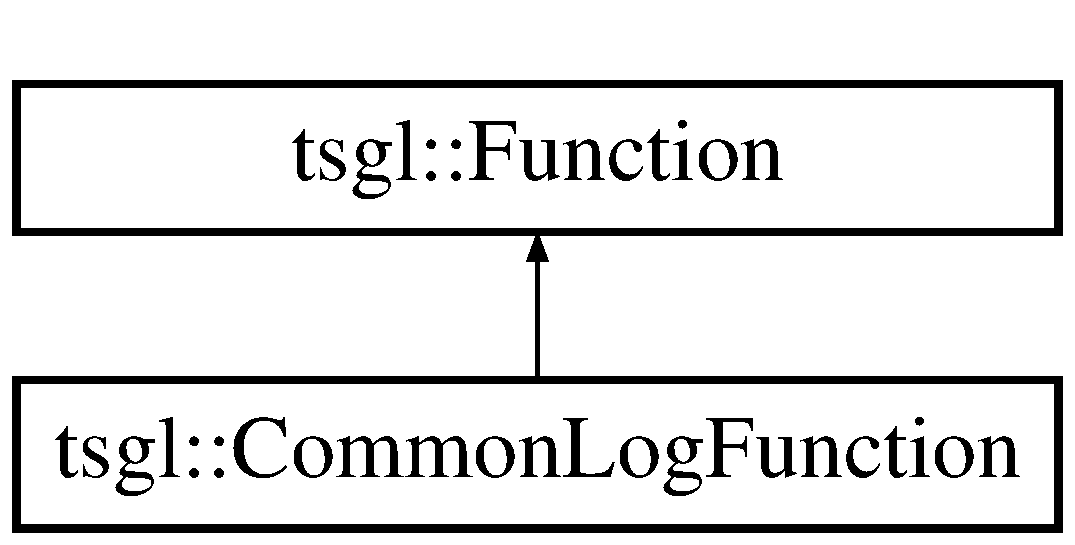
\includegraphics[height=2.000000cm]{classtsgl_1_1_common_log_function}
\end{center}
\end{figure}
\subsection*{Public Member Functions}
\begin{DoxyCompactItemize}
\item 
virtual Decimal \hyperlink{classtsgl_1_1_common_log_function_ac320c0f57c0fc4801bf8eb85f07838d8}{value\+At} (Decimal x) const 
\begin{DoxyCompactList}\small\item\em Method to determine the value of \hyperlink{classtsgl_1_1_common_log_function}{Common\+Log\+Function}. \end{DoxyCompactList}\end{DoxyCompactItemize}


\subsection{Detailed Description}
\hyperlink{classtsgl_1_1_function}{Function} to compute the base 10 log of the input. 

\subsection{Member Function Documentation}
\hypertarget{classtsgl_1_1_common_log_function_ac320c0f57c0fc4801bf8eb85f07838d8}{}\index{tsgl\+::\+Common\+Log\+Function@{tsgl\+::\+Common\+Log\+Function}!value\+At@{value\+At}}
\index{value\+At@{value\+At}!tsgl\+::\+Common\+Log\+Function@{tsgl\+::\+Common\+Log\+Function}}
\subsubsection[{value\+At}]{\setlength{\rightskip}{0pt plus 5cm}virtual Decimal tsgl\+::\+Common\+Log\+Function\+::value\+At (
\begin{DoxyParamCaption}
\item[{Decimal}]{x}
\end{DoxyParamCaption}
) const\hspace{0.3cm}{\ttfamily [inline]}, {\ttfamily [virtual]}}\label{classtsgl_1_1_common_log_function_ac320c0f57c0fc4801bf8eb85f07838d8}


Method to determine the value of \hyperlink{classtsgl_1_1_common_log_function}{Common\+Log\+Function}. 

\begin{DoxyReturn}{Returns}
The base 10 log of {\itshape x}. 
\end{DoxyReturn}


Implements \hyperlink{classtsgl_1_1_function_affb7b3b19a04efefa29a9870d666e912}{tsgl\+::\+Function}.



The documentation for this class was generated from the following file\+:\begin{DoxyCompactItemize}
\item 
Function.\+h\end{DoxyCompactItemize}

\hypertarget{classtsgl_1_1_concave_polygon}{}\section{tsgl\+:\+:Concave\+Polygon Class Reference}
\label{classtsgl_1_1_concave_polygon}\index{tsgl\+::\+Concave\+Polygon@{tsgl\+::\+Concave\+Polygon}}


Draw an arbitrary Concave polygon with colored vertices.  




{\ttfamily \#include $<$Concave\+Polygon.\+h$>$}

Inheritance diagram for tsgl\+:\+:Concave\+Polygon\+:\begin{figure}[H]
\begin{center}
\leavevmode
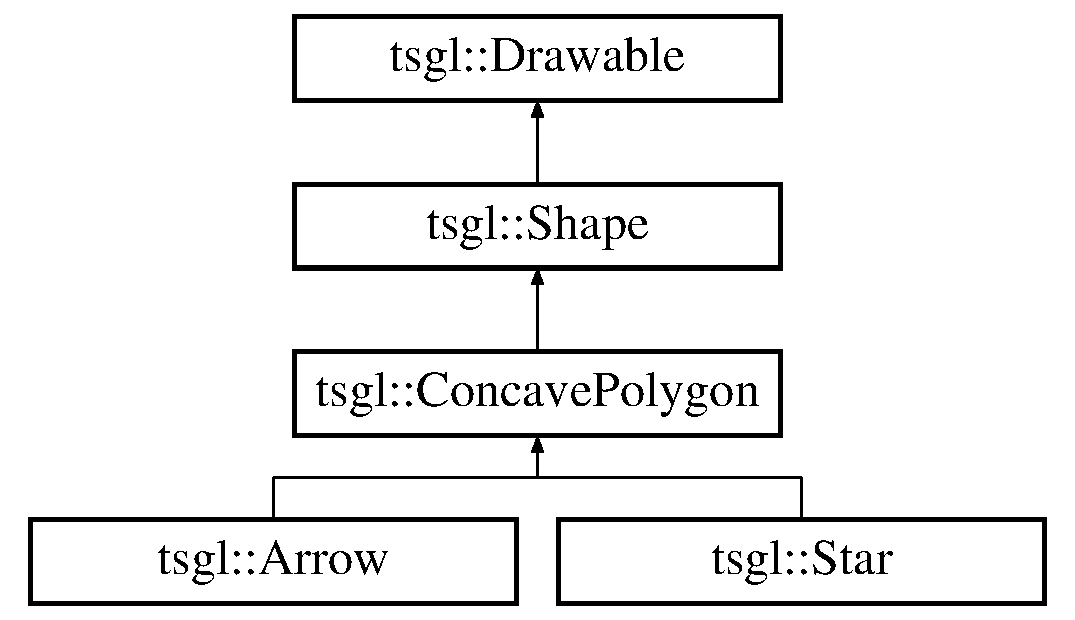
\includegraphics[height=2.000000cm]{classtsgl_1_1_concave_polygon}
\end{center}
\end{figure}
\subsection*{Public Member Functions}
\begin{DoxyCompactItemize}
\item 
\hyperlink{classtsgl_1_1_concave_polygon_a1ffb0ac20bbfa7d35683209a3c79a979}{Concave\+Polygon} (int v)
\begin{DoxyCompactList}\small\item\em Explicitly constructs a new \hyperlink{classtsgl_1_1_concave_polygon}{Concave\+Polygon}. \end{DoxyCompactList}\item 
\hyperlink{classtsgl_1_1_concave_polygon_ae1465a7135bb7ef4aa00584fa63b2530}{$\sim$\+Concave\+Polygon} ()
\begin{DoxyCompactList}\small\item\em Destroys a \hyperlink{classtsgl_1_1_concave_polygon}{Concave\+Polygon} object. \end{DoxyCompactList}\item 
bool \hyperlink{classtsgl_1_1_concave_polygon_a0fdc4936df5e1bff64031041fa84fee5}{intersects} (float p0\+\_\+x, float p0\+\_\+y, float p1\+\_\+x, float p1\+\_\+y, float p2\+\_\+x, float p2\+\_\+y, float p3\+\_\+x, float p3\+\_\+y)
\begin{DoxyCompactList}\small\item\em Determines if two lines intersect. \end{DoxyCompactList}\item 
bool \hyperlink{classtsgl_1_1_concave_polygon_afb5de38c8571d6cc808aeaec000f4522}{point\+In\+Triangle} (float px, float py, float x1, float y1, float x2, float y2, float x3, float y3)
\begin{DoxyCompactList}\small\item\em Determines whether a point resides inside of a \hyperlink{classtsgl_1_1_triangle}{Triangle}. \end{DoxyCompactList}\item 
void \hyperlink{classtsgl_1_1_concave_polygon_ae2675ff0bf54cc7092a9ab3418dcab30}{add\+Vertex} (int x, int y, const \hyperlink{structtsgl_1_1_color_float}{Color\+Float} \&color)
\begin{DoxyCompactList}\small\item\em Adds another vertex to a \hyperlink{classtsgl_1_1_concave_polygon}{Concave\+Polygon}. \end{DoxyCompactList}\item 
void \hyperlink{classtsgl_1_1_concave_polygon_a06d759932483ae2b54bb807db20cbc4a}{draw} ()
\begin{DoxyCompactList}\small\item\em Draw the \hyperlink{classtsgl_1_1_concave_polygon}{Concave\+Polygon}. \end{DoxyCompactList}\end{DoxyCompactItemize}
\subsection*{Static Public Member Functions}
\begin{DoxyCompactItemize}
\item 
static void \hyperlink{classtsgl_1_1_concave_polygon_ace68fa148735bf43d9648cb58a04ac46}{run\+Tests} ()
\begin{DoxyCompactList}\small\item\em Runs the Unit tests. \end{DoxyCompactList}\end{DoxyCompactItemize}
\subsection*{Additional Inherited Members}


\subsection{Detailed Description}
Draw an arbitrary Concave polygon with colored vertices. 

\hyperlink{classtsgl_1_1_concave_polygon}{Concave\+Polygon} is a class for holding vertex data for a triangle strip with colored vertices.

Vertices are drawn in triangle strip format, where the first three vertices make up the first triangle, the next vertex plus the previous two make up the second triangle, and so on.

This method is optimized for long lists and offers a marked improvement over drawing individual \hyperlink{classtsgl_1_1_triangle}{Triangle} instances. \begin{DoxyNote}{Note}
The \hyperlink{classtsgl_1_1_concave_polygon_ae2675ff0bf54cc7092a9ab3418dcab30}{add\+Vertex()} method must be called the same number of times as specified in the constructor. 

Calling \hyperlink{classtsgl_1_1_concave_polygon_ae2675ff0bf54cc7092a9ab3418dcab30}{add\+Vertex()} after all vertices have been added will do nothing. 

Calling \hyperlink{classtsgl_1_1_concave_polygon_a06d759932483ae2b54bb807db20cbc4a}{draw()} before all vertices have been added will do nothing. 
\end{DoxyNote}


\subsection{Constructor \& Destructor Documentation}
\hypertarget{classtsgl_1_1_concave_polygon_a1ffb0ac20bbfa7d35683209a3c79a979}{}\index{tsgl\+::\+Concave\+Polygon@{tsgl\+::\+Concave\+Polygon}!Concave\+Polygon@{Concave\+Polygon}}
\index{Concave\+Polygon@{Concave\+Polygon}!tsgl\+::\+Concave\+Polygon@{tsgl\+::\+Concave\+Polygon}}
\subsubsection[{Concave\+Polygon}]{\setlength{\rightskip}{0pt plus 5cm}tsgl\+::\+Concave\+Polygon\+::\+Concave\+Polygon (
\begin{DoxyParamCaption}
\item[{int}]{v}
\end{DoxyParamCaption}
)}\label{classtsgl_1_1_concave_polygon_a1ffb0ac20bbfa7d35683209a3c79a979}


Explicitly constructs a new \hyperlink{classtsgl_1_1_concave_polygon}{Concave\+Polygon}. 

Explicit constructor for a \hyperlink{classtsgl_1_1_concave_polygon}{Concave\+Polygon} object. 
\begin{DoxyParams}{Parameters}
{\em v} & The number of vertices the complete \hyperlink{classtsgl_1_1_concave_polygon}{Concave\+Polygon} will have. \\
\hline
\end{DoxyParams}
\begin{DoxyWarning}{Warning}
An invariant is held where if v is less than 3 then an error message is given. 
\end{DoxyWarning}
\begin{DoxyReturn}{Returns}
A new \hyperlink{classtsgl_1_1_concave_polygon}{Concave\+Polygon} with a buffer for storing the specified number of vertices. 
\end{DoxyReturn}
\hypertarget{classtsgl_1_1_concave_polygon_ae1465a7135bb7ef4aa00584fa63b2530}{}\index{tsgl\+::\+Concave\+Polygon@{tsgl\+::\+Concave\+Polygon}!````~Concave\+Polygon@{$\sim$\+Concave\+Polygon}}
\index{````~Concave\+Polygon@{$\sim$\+Concave\+Polygon}!tsgl\+::\+Concave\+Polygon@{tsgl\+::\+Concave\+Polygon}}
\subsubsection[{$\sim$\+Concave\+Polygon}]{\setlength{\rightskip}{0pt plus 5cm}tsgl\+::\+Concave\+Polygon\+::$\sim$\+Concave\+Polygon (
\begin{DoxyParamCaption}
{}
\end{DoxyParamCaption}
)}\label{classtsgl_1_1_concave_polygon_ae1465a7135bb7ef4aa00584fa63b2530}


Destroys a \hyperlink{classtsgl_1_1_concave_polygon}{Concave\+Polygon} object. 

Destructor for a \hyperlink{classtsgl_1_1_concave_polygon}{Concave\+Polygon} object.

Frees up memory that was allocated to a \hyperlink{classtsgl_1_1_concave_polygon}{Concave\+Polygon} object. 

\subsection{Member Function Documentation}
\hypertarget{classtsgl_1_1_concave_polygon_ae2675ff0bf54cc7092a9ab3418dcab30}{}\index{tsgl\+::\+Concave\+Polygon@{tsgl\+::\+Concave\+Polygon}!add\+Vertex@{add\+Vertex}}
\index{add\+Vertex@{add\+Vertex}!tsgl\+::\+Concave\+Polygon@{tsgl\+::\+Concave\+Polygon}}
\subsubsection[{add\+Vertex}]{\setlength{\rightskip}{0pt plus 5cm}void tsgl\+::\+Concave\+Polygon\+::add\+Vertex (
\begin{DoxyParamCaption}
\item[{int}]{x, }
\item[{int}]{y, }
\item[{const {\bf Color\+Float} \&}]{color}
\end{DoxyParamCaption}
)}\label{classtsgl_1_1_concave_polygon_ae2675ff0bf54cc7092a9ab3418dcab30}


Adds another vertex to a \hyperlink{classtsgl_1_1_concave_polygon}{Concave\+Polygon}. 

This function initializes the next vertex in the \hyperlink{classtsgl_1_1_polyline}{Polyline} and adds it to a \hyperlink{classtsgl_1_1_concave_polygon}{Concave\+Polygon} buffer. 
\begin{DoxyParams}{Parameters}
{\em x} & The x position of the vertex. \\
\hline
{\em y} & The y position of the vertex. \\
\hline
{\em color} & The reference variable of the color of the vertex. \\
\hline
\end{DoxyParams}
\begin{DoxyNote}{Note}
This function does nothing if the vertex buffer is already full. 

A message is given indicating that the vertex buffer is full. 
\end{DoxyNote}


Referenced by tsgl\+::\+Canvas\+::draw\+Concave\+Polygon().

\hypertarget{classtsgl_1_1_concave_polygon_a06d759932483ae2b54bb807db20cbc4a}{}\index{tsgl\+::\+Concave\+Polygon@{tsgl\+::\+Concave\+Polygon}!draw@{draw}}
\index{draw@{draw}!tsgl\+::\+Concave\+Polygon@{tsgl\+::\+Concave\+Polygon}}
\subsubsection[{draw}]{\setlength{\rightskip}{0pt plus 5cm}void tsgl\+::\+Concave\+Polygon\+::draw (
\begin{DoxyParamCaption}
{}
\end{DoxyParamCaption}
)\hspace{0.3cm}{\ttfamily [virtual]}}\label{classtsgl_1_1_concave_polygon_a06d759932483ae2b54bb807db20cbc4a}


Draw the \hyperlink{classtsgl_1_1_concave_polygon}{Concave\+Polygon}. 

This function actually draws the \hyperlink{classtsgl_1_1_concave_polygon}{Concave\+Polygon} to the \hyperlink{classtsgl_1_1_canvas}{Canvas}. \begin{DoxyNote}{Note}
This function does nothing if the vertex buffer is not yet full. 

A message is given indicating that the \hyperlink{classtsgl_1_1_concave_polygon}{Concave\+Polygon} is {\itshape N\+O\+T} ready to be drawn yet (vertex buffer = not full). 
\end{DoxyNote}
\begin{DoxyWarning}{Warning}
This is an order of n-\/cubed operation, and is thus {\bfseries V\+E\+R\+Y S\+L\+O\+W}. 
\end{DoxyWarning}


Implements \hyperlink{classtsgl_1_1_shape_af78b1627b97d621824ce86db214e2402}{tsgl\+::\+Shape}.

\hypertarget{classtsgl_1_1_concave_polygon_a0fdc4936df5e1bff64031041fa84fee5}{}\index{tsgl\+::\+Concave\+Polygon@{tsgl\+::\+Concave\+Polygon}!intersects@{intersects}}
\index{intersects@{intersects}!tsgl\+::\+Concave\+Polygon@{tsgl\+::\+Concave\+Polygon}}
\subsubsection[{intersects}]{\setlength{\rightskip}{0pt plus 5cm}bool tsgl\+::\+Concave\+Polygon\+::intersects (
\begin{DoxyParamCaption}
\item[{float}]{p0\+\_\+x, }
\item[{float}]{p0\+\_\+y, }
\item[{float}]{p1\+\_\+x, }
\item[{float}]{p1\+\_\+y, }
\item[{float}]{p2\+\_\+x, }
\item[{float}]{p2\+\_\+y, }
\item[{float}]{p3\+\_\+x, }
\item[{float}]{p3\+\_\+y}
\end{DoxyParamCaption}
)}\label{classtsgl_1_1_concave_polygon_a0fdc4936df5e1bff64031041fa84fee5}


Determines if two lines intersect. 

Simulates two lines inside of a \hyperlink{classtsgl_1_1_concave_polygon}{Concave\+Polygon} object and determines whether those two lines intersect. 
\begin{DoxyParams}{Parameters}
{\em p0\+\_\+x} & The x coordinate of the first point of the first line. \\
\hline
{\em p0\+\_\+y} & The y coordinate of the first point of the first line. \\
\hline
{\em p1\+\_\+x} & The x coordinate of the second point of the first line. \\
\hline
{\em p1\+\_\+y} & The y coordinate of the second point of the first line. \\
\hline
{\em p2\+\_\+x} & The x coordinate of the first point of the second line. \\
\hline
{\em p2\+\_\+y} & The y coordinate of the first point of the second line. \\
\hline
{\em p3\+\_\+x} & The x coordinate of the second point of the second line. \\
\hline
{\em p3\+\_\+y} & The y coordinate of the second point of the second line. \\
\hline
\end{DoxyParams}
\begin{DoxyReturn}{Returns}
true if the lines do intersect, false if otherwise. 
\end{DoxyReturn}


Referenced by draw().

\hypertarget{classtsgl_1_1_concave_polygon_afb5de38c8571d6cc808aeaec000f4522}{}\index{tsgl\+::\+Concave\+Polygon@{tsgl\+::\+Concave\+Polygon}!point\+In\+Triangle@{point\+In\+Triangle}}
\index{point\+In\+Triangle@{point\+In\+Triangle}!tsgl\+::\+Concave\+Polygon@{tsgl\+::\+Concave\+Polygon}}
\subsubsection[{point\+In\+Triangle}]{\setlength{\rightskip}{0pt plus 5cm}bool tsgl\+::\+Concave\+Polygon\+::point\+In\+Triangle (
\begin{DoxyParamCaption}
\item[{float}]{px, }
\item[{float}]{py, }
\item[{float}]{x1, }
\item[{float}]{y1, }
\item[{float}]{x2, }
\item[{float}]{y2, }
\item[{float}]{x3, }
\item[{float}]{y3}
\end{DoxyParamCaption}
)}\label{classtsgl_1_1_concave_polygon_afb5de38c8571d6cc808aeaec000f4522}


Determines whether a point resides inside of a \hyperlink{classtsgl_1_1_triangle}{Triangle}. 

Simulates a \hyperlink{classtsgl_1_1_triangle}{Triangle} and point inside of a \hyperlink{classtsgl_1_1_concave_polygon}{Concave\+Polygon} object and determines whether the point resides inside of the \hyperlink{classtsgl_1_1_triangle}{Triangle}. 
\begin{DoxyParams}{Parameters}
{\em px} & The x coordinate of the point. \\
\hline
{\em py} & The y coordinate of the point. \\
\hline
{\em x1} & The x coordinate of the first vertex of the \hyperlink{classtsgl_1_1_triangle}{Triangle}. \\
\hline
{\em y1} & The y coordinate of the first vertex of the \hyperlink{classtsgl_1_1_triangle}{Triangle}. \\
\hline
{\em x2} & The x coordinate of the second vertex of the \hyperlink{classtsgl_1_1_triangle}{Triangle}. \\
\hline
{\em y2} & The y coordinate of the second vertex of the \hyperlink{classtsgl_1_1_triangle}{Triangle}. \\
\hline
{\em x3} & The x coordinate of the third vertex of the \hyperlink{classtsgl_1_1_triangle}{Triangle}. \\
\hline
{\em y3} & The y coordinate of the third vertex of the \hyperlink{classtsgl_1_1_triangle}{Triangle}. \\
\hline
\end{DoxyParams}
\begin{DoxyReturn}{Returns}
true if the point does reside in the \hyperlink{classtsgl_1_1_triangle}{Triangle}, false if otherwise. 
\end{DoxyReturn}


Referenced by draw().

\hypertarget{classtsgl_1_1_concave_polygon_ace68fa148735bf43d9648cb58a04ac46}{}\index{tsgl\+::\+Concave\+Polygon@{tsgl\+::\+Concave\+Polygon}!run\+Tests@{run\+Tests}}
\index{run\+Tests@{run\+Tests}!tsgl\+::\+Concave\+Polygon@{tsgl\+::\+Concave\+Polygon}}
\subsubsection[{run\+Tests}]{\setlength{\rightskip}{0pt plus 5cm}void tsgl\+::\+Concave\+Polygon\+::run\+Tests (
\begin{DoxyParamCaption}
{}
\end{DoxyParamCaption}
)\hspace{0.3cm}{\ttfamily [static]}}\label{classtsgl_1_1_concave_polygon_ace68fa148735bf43d9648cb58a04ac46}


Runs the Unit tests. 

Runs the Unit tests for the \hyperlink{classtsgl_1_1_concave_polygon}{Concave\+Polygon} class. \hyperlink{classtsgl_1_1_concave_polygon_a0fdc4936df5e1bff64031041fa84fee5}{intersects()} and \hyperlink{classtsgl_1_1_concave_polygon_afb5de38c8571d6cc808aeaec000f4522}{point\+In\+Triangle()} are tested. 

The documentation for this class was generated from the following files\+:\begin{DoxyCompactItemize}
\item 
Concave\+Polygon.\+h\item 
Concave\+Polygon.\+cpp\end{DoxyCompactItemize}

\hypertarget{classtsgl_1_1_cone}{}\section{tsgl\+:\+:Cone Class Reference}
\label{classtsgl_1_1_cone}\index{tsgl\+::\+Cone@{tsgl\+::\+Cone}}


Draw an arbitrary \hyperlink{classtsgl_1_1_cone}{Cone} with colored vertices.  




{\ttfamily \#include $<$Cone.\+h$>$}

Inheritance diagram for tsgl\+:\+:Cone\+:\begin{figure}[H]
\begin{center}
\leavevmode
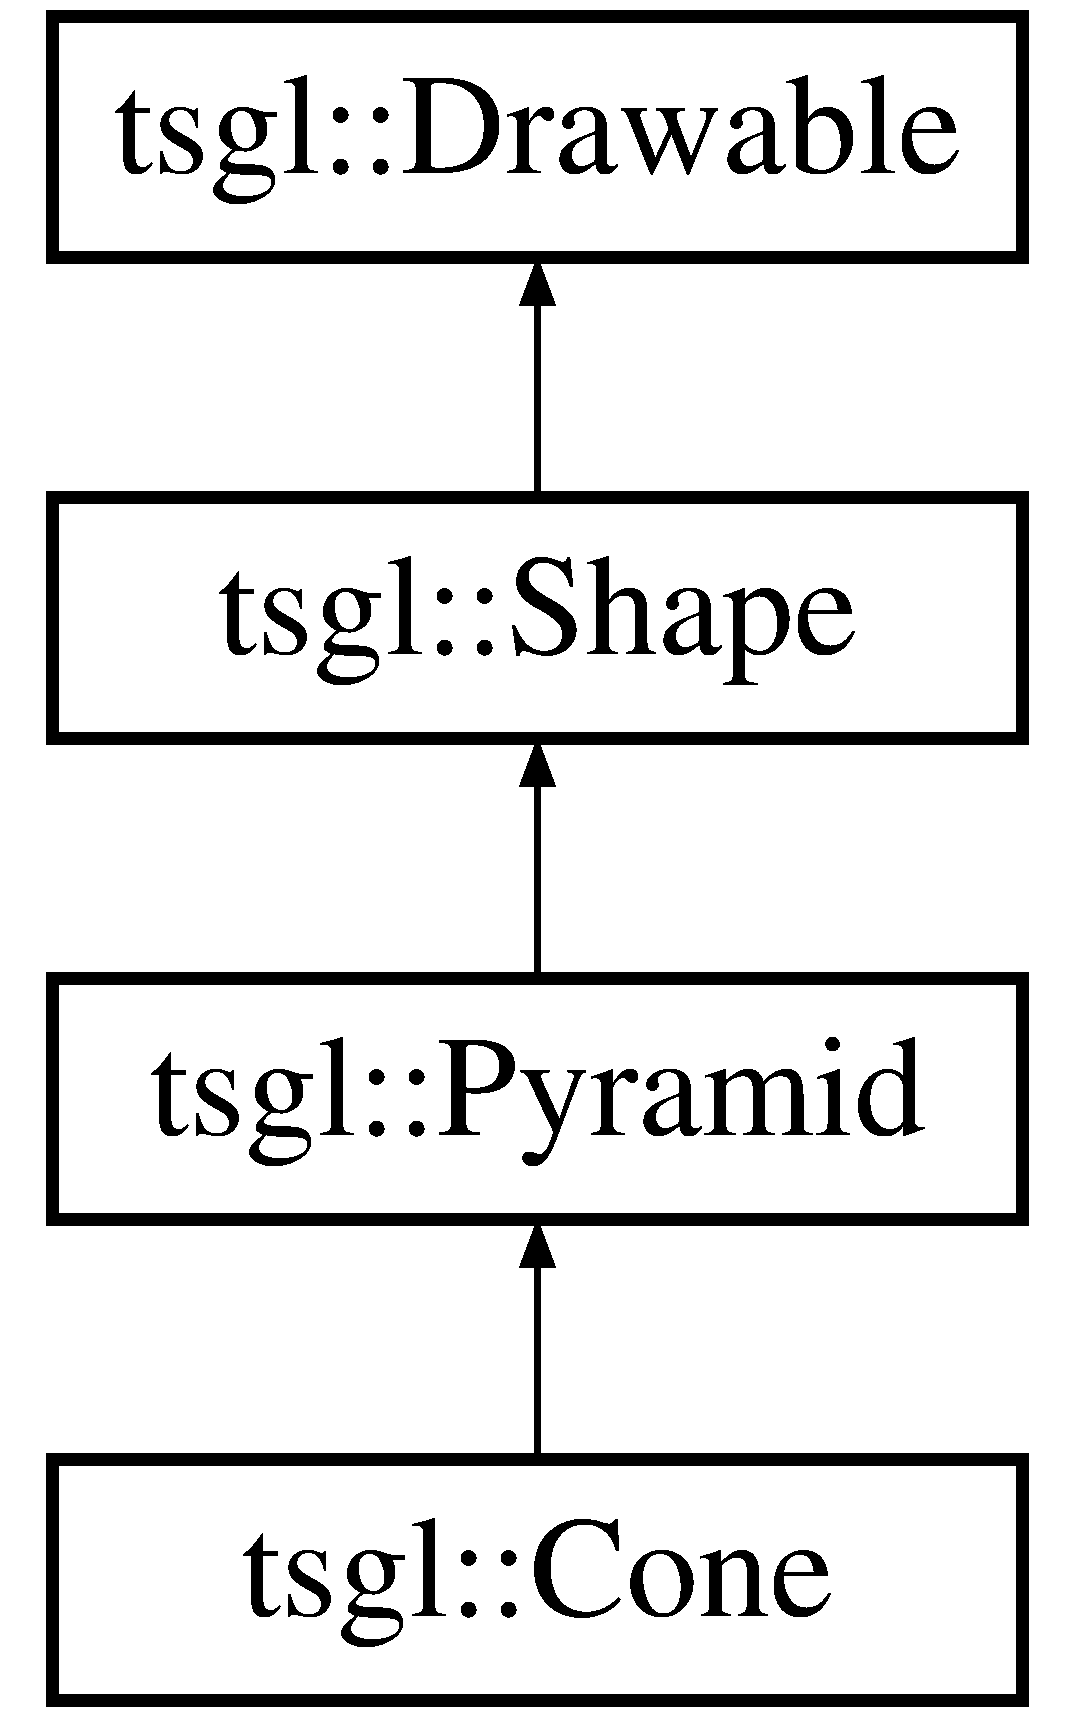
\includegraphics[height=4.000000cm]{classtsgl_1_1_cone}
\end{center}
\end{figure}
\subsection*{Public Member Functions}
\begin{DoxyCompactItemize}
\item 
\hyperlink{classtsgl_1_1_cone_a1bbc50a0f701f7124426d62ef3cfc6d7}{Cone} (float x, float y, float z, float height, float radius, float yaw, float pitch, float roll, \hyperlink{structtsgl_1_1_color_float}{Color\+Float} c)
\begin{DoxyCompactList}\small\item\em Explicitly constructs a new \hyperlink{classtsgl_1_1_cone}{Cone}. \end{DoxyCompactList}\item 
\hyperlink{classtsgl_1_1_cone_aabdb5094d21ce830a5a08893b51c5bc5}{Cone} (float x, float y, float z, float height, float radius, float yaw, float pitch, float roll, \hyperlink{structtsgl_1_1_color_float}{Color\+Float} c\mbox{[}$\,$\mbox{]})
\begin{DoxyCompactList}\small\item\em Explicitly constructs a new \hyperlink{classtsgl_1_1_cone}{Cone}. \end{DoxyCompactList}\item 
\mbox{\Hypertarget{classtsgl_1_1_cone_ac6611697b725375106016762f1cafc48}\label{classtsgl_1_1_cone_ac6611697b725375106016762f1cafc48}} 
virtual \hyperlink{classtsgl_1_1_cone_ac6611697b725375106016762f1cafc48}{$\sim$\+Cone} ()
\begin{DoxyCompactList}\small\item\em Destructor for the \hyperlink{classtsgl_1_1_cone}{Cone}. \end{DoxyCompactList}\end{DoxyCompactItemize}
\subsection*{Additional Inherited Members}


\subsection{Detailed Description}
Draw an arbitrary \hyperlink{classtsgl_1_1_cone}{Cone} with colored vertices. 

\hyperlink{classtsgl_1_1_cone}{Cone} is a class for holding vertex data for a cone.

\hyperlink{classtsgl_1_1_cone}{Cone} is a subclass of \hyperlink{classtsgl_1_1_pyramid}{Pyramid} with a base of (radius $\ast$ 3) sides, minimum of 3. 

\subsection{Constructor \& Destructor Documentation}
\mbox{\Hypertarget{classtsgl_1_1_cone_a1bbc50a0f701f7124426d62ef3cfc6d7}\label{classtsgl_1_1_cone_a1bbc50a0f701f7124426d62ef3cfc6d7}} 
\index{tsgl\+::\+Cone@{tsgl\+::\+Cone}!Cone@{Cone}}
\index{Cone@{Cone}!tsgl\+::\+Cone@{tsgl\+::\+Cone}}
\subsubsection{\texorpdfstring{Cone()}{Cone()}\hspace{0.1cm}{\footnotesize\ttfamily [1/2]}}
{\footnotesize\ttfamily tsgl\+::\+Cone\+::\+Cone (\begin{DoxyParamCaption}\item[{float}]{x,  }\item[{float}]{y,  }\item[{float}]{z,  }\item[{float}]{height,  }\item[{float}]{radius,  }\item[{float}]{yaw,  }\item[{float}]{pitch,  }\item[{float}]{roll,  }\item[{\hyperlink{structtsgl_1_1_color_float}{Color\+Float}}]{c }\end{DoxyParamCaption})}



Explicitly constructs a new \hyperlink{classtsgl_1_1_cone}{Cone}. 

Explicit constructor for a \hyperlink{classtsgl_1_1_cone}{Cone} object. 
\begin{DoxyParams}{Parameters}
{\em x} & The x coordinate of the center of the \hyperlink{classtsgl_1_1_cone}{Cone}. \\
\hline
{\em y} & The y coordinate of the center of the \hyperlink{classtsgl_1_1_cone}{Cone}. \\
\hline
{\em z} & The z coordinate of the center of the \hyperlink{classtsgl_1_1_cone}{Cone}. \\
\hline
{\em height} & The distance from the center of the base to tip of the \hyperlink{classtsgl_1_1_cone}{Cone}. \\
\hline
{\em radius} & The radius of the \hyperlink{classtsgl_1_1_cone}{Cone}\textquotesingle{}s circular base. \\
\hline
{\em yaw} & The \hyperlink{classtsgl_1_1_cone}{Cone}\textquotesingle{}s yaw. \\
\hline
{\em pitch} & The \hyperlink{classtsgl_1_1_cone}{Cone}\textquotesingle{}s pitch. \\
\hline
{\em roll} & The \hyperlink{classtsgl_1_1_cone}{Cone}\textquotesingle{}s roll. \\
\hline
{\em c} & A \hyperlink{structtsgl_1_1_color_float}{Color\+Float} for the \hyperlink{classtsgl_1_1_cone}{Cone}\textquotesingle{}s vertex colors. \\
\hline
\end{DoxyParams}
\begin{DoxyWarning}{Warning}
An invariant is held where if radius isn\textquotesingle{}t positive then an error message is given. 
\end{DoxyWarning}
\begin{DoxyReturn}{Returns}
A new \hyperlink{classtsgl_1_1_cone}{Cone} with a buffer for storing the specified numbered of vertices. 
\end{DoxyReturn}
\mbox{\Hypertarget{classtsgl_1_1_cone_aabdb5094d21ce830a5a08893b51c5bc5}\label{classtsgl_1_1_cone_aabdb5094d21ce830a5a08893b51c5bc5}} 
\index{tsgl\+::\+Cone@{tsgl\+::\+Cone}!Cone@{Cone}}
\index{Cone@{Cone}!tsgl\+::\+Cone@{tsgl\+::\+Cone}}
\subsubsection{\texorpdfstring{Cone()}{Cone()}\hspace{0.1cm}{\footnotesize\ttfamily [2/2]}}
{\footnotesize\ttfamily tsgl\+::\+Cone\+::\+Cone (\begin{DoxyParamCaption}\item[{float}]{x,  }\item[{float}]{y,  }\item[{float}]{z,  }\item[{float}]{height,  }\item[{float}]{radius,  }\item[{float}]{yaw,  }\item[{float}]{pitch,  }\item[{float}]{roll,  }\item[{\hyperlink{structtsgl_1_1_color_float}{Color\+Float}}]{c\mbox{[}$\,$\mbox{]} }\end{DoxyParamCaption})}



Explicitly constructs a new \hyperlink{classtsgl_1_1_cone}{Cone}. 

Explicit constructor for a \hyperlink{classtsgl_1_1_cone}{Cone} object. 
\begin{DoxyParams}{Parameters}
{\em x} & The x coordinate of the center of the \hyperlink{classtsgl_1_1_cone}{Cone}. \\
\hline
{\em y} & The y coordinate of the center of the \hyperlink{classtsgl_1_1_cone}{Cone}. \\
\hline
{\em z} & The z coordinate of the center of the \hyperlink{classtsgl_1_1_cone}{Cone}. \\
\hline
{\em height} & The distance from the center of the base to tip of the \hyperlink{classtsgl_1_1_cone}{Cone}. \\
\hline
{\em radius} & The radius of the \hyperlink{classtsgl_1_1_cone}{Cone}\textquotesingle{}s circular base. \\
\hline
{\em yaw} & The \hyperlink{classtsgl_1_1_cone}{Cone}\textquotesingle{}s yaw. \\
\hline
{\em pitch} & The \hyperlink{classtsgl_1_1_cone}{Cone}\textquotesingle{}s pitch. \\
\hline
{\em roll} & The \hyperlink{classtsgl_1_1_cone}{Cone}\textquotesingle{}s roll. \\
\hline
{\em c} & An array of Color\+Floats containing the \hyperlink{classtsgl_1_1_cone}{Cone}\textquotesingle{}s vertex colors. \\
\hline
\end{DoxyParams}
\begin{DoxyWarning}{Warning}
An invariant is held where if radius isn\textquotesingle{}t positive then an error message is given. 
\end{DoxyWarning}
\begin{DoxyReturn}{Returns}
A new \hyperlink{classtsgl_1_1_cone}{Cone} with a buffer for storing the specified numbered of vertices. 
\end{DoxyReturn}


The documentation for this class was generated from the following files\+:\begin{DoxyCompactItemize}
\item 
Cone.\+h\item 
Cone.\+cpp\end{DoxyCompactItemize}

\hypertarget{class_consumer}{}\section{Consumer Class Reference}
\label{class_consumer}\index{Consumer@{Consumer}}


{\ttfamily \#include $<$Consumer.\+h$>$}

Inheritance diagram for Consumer\+:\begin{figure}[H]
\begin{center}
\leavevmode
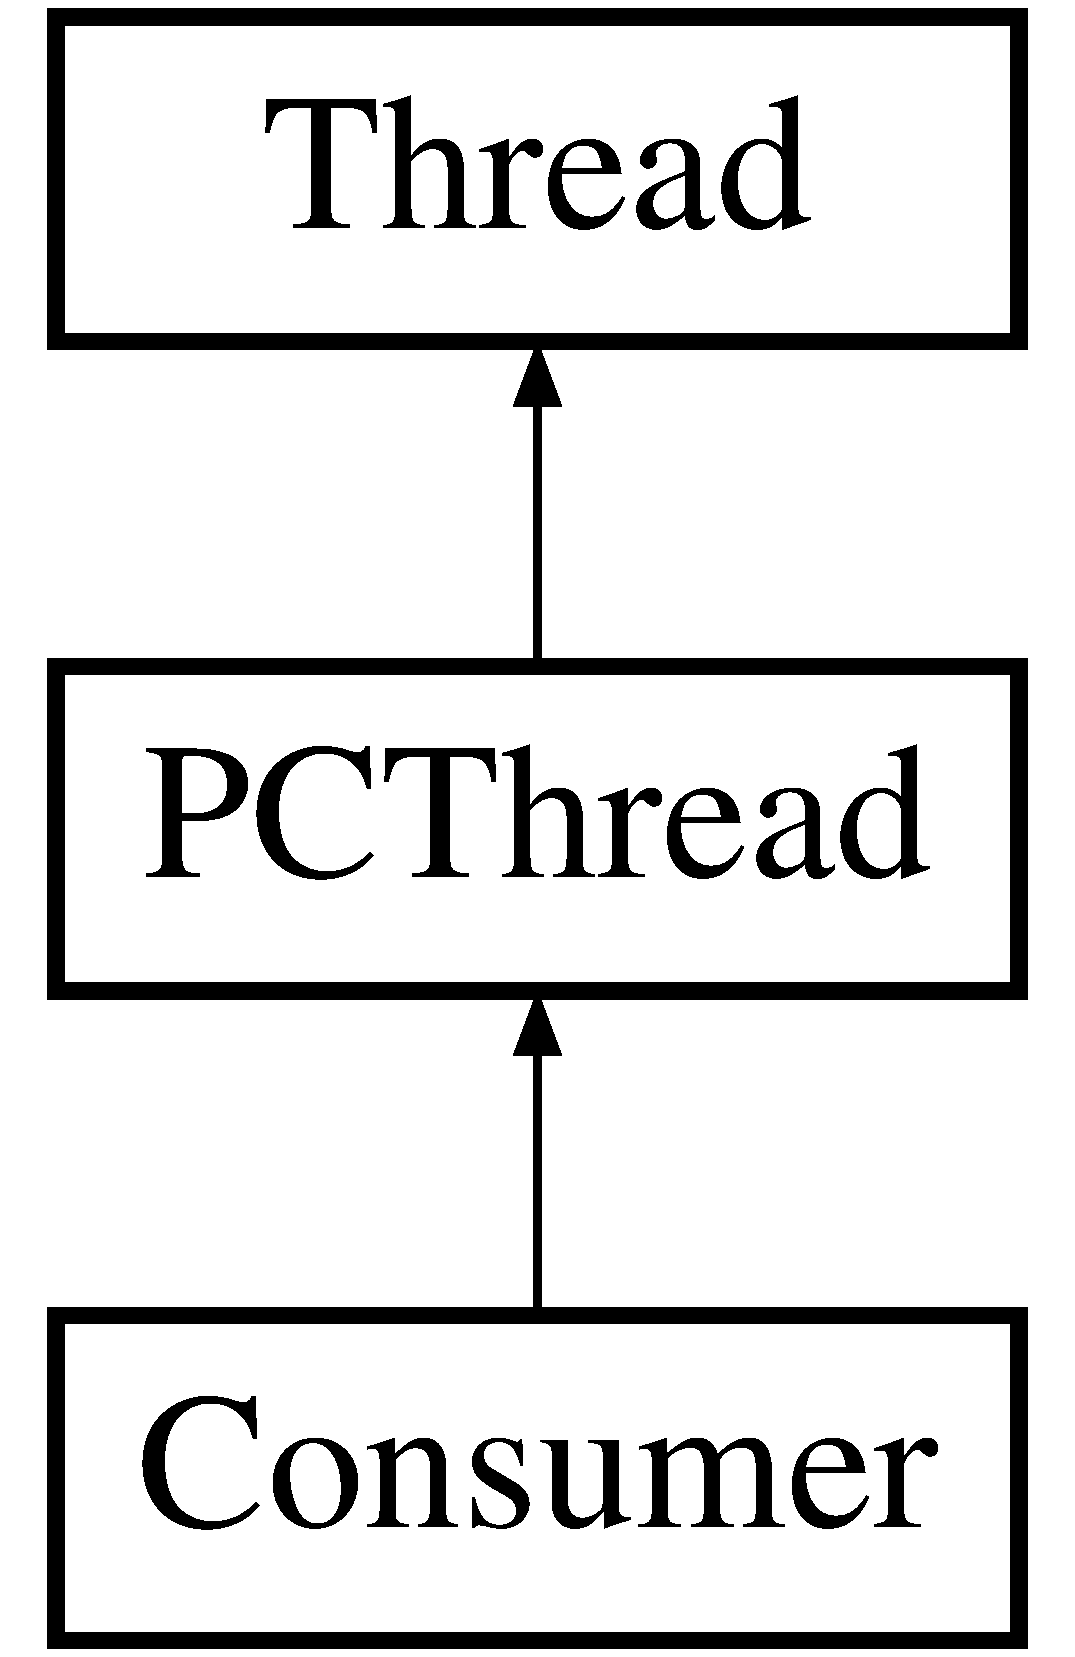
\includegraphics[height=3.000000cm]{class_consumer}
\end{center}
\end{figure}
\subsection*{Public Member Functions}
\begin{DoxyCompactItemize}
\item 
\hyperlink{class_consumer_a31a7b4bc675d04c877269a5da93b981a}{Consumer} ()
\item 
\hyperlink{class_consumer_a8297e8de091856b95132502fa4a4ab44}{Consumer} (\hyperlink{class_queue}{Queue}$<$ \hyperlink{classtsgl_1_1_star}{Star} $\ast$$>$ \&shared\+Buffer, unsigned long id, \hyperlink{classtsgl_1_1_canvas}{Canvas} \&can)
\item 
void \hyperlink{class_consumer_a58ab6de26dfe34d59c0522fff19f1abf}{lock} ()
\item 
void \hyperlink{class_consumer_a759bbf618e780c1cca3f7a5136d3c910}{act} ()
\item 
void \hyperlink{class_consumer_acf783a2789b071a237f7759ccf6bacaf}{unlock} ()
\end{DoxyCompactItemize}
\subsection*{Additional Inherited Members}


\subsection{Detailed Description}
\hyperlink{class_consumer}{Consumer} class inherits from the \hyperlink{class_thread}{Thread} class in order to create a \hyperlink{class_consumer}{Consumer} object. Inheritance\+: \hyperlink{class_thread}{Thread} class. Implements the run() method, which calls the consume() method. 

\subsection{Constructor \& Destructor Documentation}
\mbox{\Hypertarget{class_consumer_a31a7b4bc675d04c877269a5da93b981a}\label{class_consumer_a31a7b4bc675d04c877269a5da93b981a}} 
\index{Consumer@{Consumer}!Consumer@{Consumer}}
\index{Consumer@{Consumer}!Consumer@{Consumer}}
\subsubsection{\texorpdfstring{Consumer()}{Consumer()}\hspace{0.1cm}{\footnotesize\ttfamily [1/2]}}
{\footnotesize\ttfamily Consumer\+::\+Consumer (\begin{DoxyParamCaption}{ }\end{DoxyParamCaption})}

Default-\/constructor for the \hyperlink{class_consumer}{Consumer} class. return\+: The constructed \hyperlink{class_consumer}{Consumer} object. \mbox{\Hypertarget{class_consumer_a8297e8de091856b95132502fa4a4ab44}\label{class_consumer_a8297e8de091856b95132502fa4a4ab44}} 
\index{Consumer@{Consumer}!Consumer@{Consumer}}
\index{Consumer@{Consumer}!Consumer@{Consumer}}
\subsubsection{\texorpdfstring{Consumer()}{Consumer()}\hspace{0.1cm}{\footnotesize\ttfamily [2/2]}}
{\footnotesize\ttfamily Consumer\+::\+Consumer (\begin{DoxyParamCaption}\item[{\hyperlink{class_queue}{Queue}$<$ \hyperlink{classtsgl_1_1_star}{Star} $\ast$$>$ \&}]{shared\+Buffer,  }\item[{unsigned long}]{id,  }\item[{\hyperlink{classtsgl_1_1_canvas}{Canvas} \&}]{can }\end{DoxyParamCaption})}

Explicit-\/constructor for the \hyperlink{class_consumer}{Consumer} class. param\+: shared\+Buffer, a reference to the \hyperlink{class_queue}{Queue} object that is shared between the \hyperlink{class_consumer}{Consumer} and \hyperlink{class_producer}{Producer}. param\+: id, an unsigned long that will be passed to the \hyperlink{class_thread_a95c703fb8f2f27cb64f475a8c940864a}{Thread()} constructor that will act as the id for the \hyperlink{class_thread}{Thread} object. param\+: can, a handle to the Canvas that will be drawn on and will determine whether or not to continue consuming object from the \hyperlink{class_queue}{Queue}. return\+: The constructed \hyperlink{class_consumer}{Consumer} object. 

\subsection{Member Function Documentation}
\mbox{\Hypertarget{class_consumer_a759bbf618e780c1cca3f7a5136d3c910}\label{class_consumer_a759bbf618e780c1cca3f7a5136d3c910}} 
\index{Consumer@{Consumer}!act@{act}}
\index{act@{act}!Consumer@{Consumer}}
\subsubsection{\texorpdfstring{act()}{act()}}
{\footnotesize\ttfamily void Consumer\+::act (\begin{DoxyParamCaption}{ }\end{DoxyParamCaption})\hspace{0.3cm}{\ttfamily [virtual]}}

act goes through the process of consuming an item from \hyperlink{class_queue}{Queue} 

Implements \hyperlink{class_p_c_thread}{P\+C\+Thread}.

\mbox{\Hypertarget{class_consumer_a58ab6de26dfe34d59c0522fff19f1abf}\label{class_consumer_a58ab6de26dfe34d59c0522fff19f1abf}} 
\index{Consumer@{Consumer}!lock@{lock}}
\index{lock@{lock}!Consumer@{Consumer}}
\subsubsection{\texorpdfstring{lock()}{lock()}}
{\footnotesize\ttfamily void Consumer\+::lock (\begin{DoxyParamCaption}{ }\end{DoxyParamCaption})\hspace{0.3cm}{\ttfamily [virtual]}}

locks the \hyperlink{class_queue}{Queue} for consumption 

Implements \hyperlink{class_p_c_thread}{P\+C\+Thread}.

\mbox{\Hypertarget{class_consumer_acf783a2789b071a237f7759ccf6bacaf}\label{class_consumer_acf783a2789b071a237f7759ccf6bacaf}} 
\index{Consumer@{Consumer}!unlock@{unlock}}
\index{unlock@{unlock}!Consumer@{Consumer}}
\subsubsection{\texorpdfstring{unlock()}{unlock()}}
{\footnotesize\ttfamily void Consumer\+::unlock (\begin{DoxyParamCaption}{ }\end{DoxyParamCaption})\hspace{0.3cm}{\ttfamily [virtual]}}

unlocks the \hyperlink{class_queue}{Queue} after consuming an item 

Implements \hyperlink{class_p_c_thread}{P\+C\+Thread}.



The documentation for this class was generated from the following files\+:\begin{DoxyCompactItemize}
\item 
/home/sth5/test/\+T\+S\+G\+L/src/examples/\+Producer\+Consumer/Consumer.\+h\item 
/home/sth5/test/\+T\+S\+G\+L/src/examples/\+Producer\+Consumer/Consumer.\+cpp\end{DoxyCompactItemize}

\hypertarget{classtsgl_1_1_convex_polygon}{}\section{tsgl\+:\+:Convex\+Polygon Class Reference}
\label{classtsgl_1_1_convex_polygon}\index{tsgl\+::\+Convex\+Polygon@{tsgl\+::\+Convex\+Polygon}}


Draw an arbitrary Convex polygon with colored vertices.  




{\ttfamily \#include $<$Convex\+Polygon.\+h$>$}

Inheritance diagram for tsgl\+:\+:Convex\+Polygon\+:\begin{figure}[H]
\begin{center}
\leavevmode
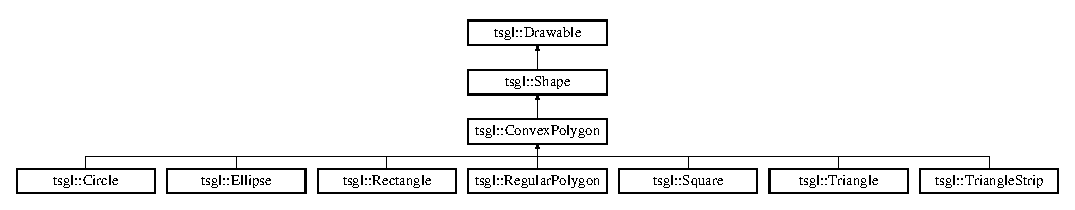
\includegraphics[height=2.000000cm]{classtsgl_1_1_convex_polygon}
\end{center}
\end{figure}
\subsection*{Public Member Functions}
\begin{DoxyCompactItemize}
\item 
\hyperlink{classtsgl_1_1_convex_polygon_a4ae2bd47b2a9f89aec5906c4e7ae3c10}{Convex\+Polygon} (int v)
\begin{DoxyCompactList}\small\item\em Explicitly constructs a new \hyperlink{classtsgl_1_1_convex_polygon}{Convex\+Polygon}. \end{DoxyCompactList}\item 
\hyperlink{classtsgl_1_1_convex_polygon_a46a5bde76d6843d47c754a04cc847e64}{$\sim$\+Convex\+Polygon} ()
\begin{DoxyCompactList}\small\item\em Destroys a \hyperlink{classtsgl_1_1_convex_polygon}{Convex\+Polygon} object. \end{DoxyCompactList}\item 
void \hyperlink{classtsgl_1_1_convex_polygon_a60d17a5ac80a796d05dfeff855791cc0}{add\+Vertex} (int x, int y, const \hyperlink{structtsgl_1_1_color_float}{Color\+Float} \&color)
\begin{DoxyCompactList}\small\item\em Adds another vertex to a \hyperlink{classtsgl_1_1_convex_polygon}{Convex\+Polygon}. \end{DoxyCompactList}\item 
void \hyperlink{classtsgl_1_1_convex_polygon_add4d4971a5d22385eebbfe771af916b5}{draw} ()
\begin{DoxyCompactList}\small\item\em Draw the \hyperlink{classtsgl_1_1_convex_polygon}{Convex\+Polygon}. \end{DoxyCompactList}\end{DoxyCompactItemize}
\subsection*{Static Public Member Functions}
\begin{DoxyCompactItemize}
\item 
static void \hyperlink{classtsgl_1_1_convex_polygon_ac309bc2b2f142b0a02b9dc38e901daeb}{run\+Tests} ()
\begin{DoxyCompactList}\small\item\em Runs the Unit tests. \end{DoxyCompactList}\end{DoxyCompactItemize}
\subsection*{Additional Inherited Members}


\subsection{Detailed Description}
Draw an arbitrary Convex polygon with colored vertices. 

\hyperlink{classtsgl_1_1_convex_polygon}{Convex\+Polygon} is a class for holding vertex data for a triangle strip with colored vertices.

Vertices are drawn in triangle strip format, where the first three vertices make up the first triangle, the next vertex plus the previous two make up the second triangle, and so on.

This method is optimized for long lists and offers a marked improvement over drawing individual \hyperlink{classtsgl_1_1_triangle}{Triangle} instances. \begin{DoxyNote}{Note}
The \hyperlink{classtsgl_1_1_convex_polygon_a60d17a5ac80a796d05dfeff855791cc0}{add\+Vertex()} method must be called the same number of times as specified in the constructor. 

Calling \hyperlink{classtsgl_1_1_convex_polygon_a60d17a5ac80a796d05dfeff855791cc0}{add\+Vertex()} after all vertices have been added will do nothing. 

Calling \hyperlink{classtsgl_1_1_convex_polygon_add4d4971a5d22385eebbfe771af916b5}{draw()} before all vertices have been added will do nothing. 
\end{DoxyNote}


\subsection{Constructor \& Destructor Documentation}
\hypertarget{classtsgl_1_1_convex_polygon_a4ae2bd47b2a9f89aec5906c4e7ae3c10}{}\index{tsgl\+::\+Convex\+Polygon@{tsgl\+::\+Convex\+Polygon}!Convex\+Polygon@{Convex\+Polygon}}
\index{Convex\+Polygon@{Convex\+Polygon}!tsgl\+::\+Convex\+Polygon@{tsgl\+::\+Convex\+Polygon}}
\subsubsection[{Convex\+Polygon}]{\setlength{\rightskip}{0pt plus 5cm}tsgl\+::\+Convex\+Polygon\+::\+Convex\+Polygon (
\begin{DoxyParamCaption}
\item[{int}]{v}
\end{DoxyParamCaption}
)}\label{classtsgl_1_1_convex_polygon_a4ae2bd47b2a9f89aec5906c4e7ae3c10}


Explicitly constructs a new \hyperlink{classtsgl_1_1_convex_polygon}{Convex\+Polygon}. 

Explicit constructor for a Convex Polygon object. 
\begin{DoxyParams}{Parameters}
{\em v} & the number of vertices the complete \hyperlink{classtsgl_1_1_convex_polygon}{Convex\+Polygon} will have. \\
\hline
\end{DoxyParams}
\begin{DoxyWarning}{Warning}
An invariant is held where if v is less than 3 then an error message is given. 
\end{DoxyWarning}
\begin{DoxyReturn}{Returns}
A new \hyperlink{classtsgl_1_1_convex_polygon}{Convex\+Polygon} with a buffer for storing the specified numbered of vertices. 
\end{DoxyReturn}
\hypertarget{classtsgl_1_1_convex_polygon_a46a5bde76d6843d47c754a04cc847e64}{}\index{tsgl\+::\+Convex\+Polygon@{tsgl\+::\+Convex\+Polygon}!````~Convex\+Polygon@{$\sim$\+Convex\+Polygon}}
\index{````~Convex\+Polygon@{$\sim$\+Convex\+Polygon}!tsgl\+::\+Convex\+Polygon@{tsgl\+::\+Convex\+Polygon}}
\subsubsection[{$\sim$\+Convex\+Polygon}]{\setlength{\rightskip}{0pt plus 5cm}tsgl\+::\+Convex\+Polygon\+::$\sim$\+Convex\+Polygon (
\begin{DoxyParamCaption}
{}
\end{DoxyParamCaption}
)}\label{classtsgl_1_1_convex_polygon_a46a5bde76d6843d47c754a04cc847e64}


Destroys a \hyperlink{classtsgl_1_1_convex_polygon}{Convex\+Polygon} object. 

Destructor for a \hyperlink{classtsgl_1_1_convex_polygon}{Convex\+Polygon}.

Frees up memory that was allocated to a \hyperlink{classtsgl_1_1_convex_polygon}{Convex\+Polygon} object. 

\subsection{Member Function Documentation}
\hypertarget{classtsgl_1_1_convex_polygon_a60d17a5ac80a796d05dfeff855791cc0}{}\index{tsgl\+::\+Convex\+Polygon@{tsgl\+::\+Convex\+Polygon}!add\+Vertex@{add\+Vertex}}
\index{add\+Vertex@{add\+Vertex}!tsgl\+::\+Convex\+Polygon@{tsgl\+::\+Convex\+Polygon}}
\subsubsection[{add\+Vertex}]{\setlength{\rightskip}{0pt plus 5cm}void tsgl\+::\+Convex\+Polygon\+::add\+Vertex (
\begin{DoxyParamCaption}
\item[{int}]{x, }
\item[{int}]{y, }
\item[{const {\bf Color\+Float} \&}]{color}
\end{DoxyParamCaption}
)}\label{classtsgl_1_1_convex_polygon_a60d17a5ac80a796d05dfeff855791cc0}


Adds another vertex to a \hyperlink{classtsgl_1_1_convex_polygon}{Convex\+Polygon}. 

This function initializes the next vertex in the \hyperlink{classtsgl_1_1_polyline}{Polyline} and adds it to a \hyperlink{classtsgl_1_1_convex_polygon}{Convex\+Polygon} buffer. 
\begin{DoxyParams}{Parameters}
{\em x} & The x position of the vertex. \\
\hline
{\em y} & The y position of the vertex. \\
\hline
{\em color} & The reference variable of the color of the vertex. \\
\hline
\end{DoxyParams}
\begin{DoxyNote}{Note}
This function does nothing if the vertex buffer is already full. 

A message is given indicating when the vertex buffer is full. 
\end{DoxyNote}


Referenced by tsgl\+::\+Canvas\+::draw\+Circle(), and tsgl\+::\+Canvas\+::draw\+Convex\+Polygon().

\hypertarget{classtsgl_1_1_convex_polygon_add4d4971a5d22385eebbfe771af916b5}{}\index{tsgl\+::\+Convex\+Polygon@{tsgl\+::\+Convex\+Polygon}!draw@{draw}}
\index{draw@{draw}!tsgl\+::\+Convex\+Polygon@{tsgl\+::\+Convex\+Polygon}}
\subsubsection[{draw}]{\setlength{\rightskip}{0pt plus 5cm}void tsgl\+::\+Convex\+Polygon\+::draw (
\begin{DoxyParamCaption}
{}
\end{DoxyParamCaption}
)\hspace{0.3cm}{\ttfamily [virtual]}}\label{classtsgl_1_1_convex_polygon_add4d4971a5d22385eebbfe771af916b5}


Draw the \hyperlink{classtsgl_1_1_convex_polygon}{Convex\+Polygon}. 

This function actually draws the \hyperlink{classtsgl_1_1_convex_polygon}{Convex\+Polygon} to the \hyperlink{classtsgl_1_1_canvas}{Canvas}. \begin{DoxyNote}{Note}
This function does nothing if the vertex buffer is not yet full. 

A message is given indicating that the \hyperlink{classtsgl_1_1_convex_polygon}{Convex\+Polygon} is {\itshape N\+O\+T} ready to be drawn yet (vertex buffer = not full). 
\end{DoxyNote}


Implements \hyperlink{classtsgl_1_1_shape_af78b1627b97d621824ce86db214e2402}{tsgl\+::\+Shape}.

\hypertarget{classtsgl_1_1_convex_polygon_ac309bc2b2f142b0a02b9dc38e901daeb}{}\index{tsgl\+::\+Convex\+Polygon@{tsgl\+::\+Convex\+Polygon}!run\+Tests@{run\+Tests}}
\index{run\+Tests@{run\+Tests}!tsgl\+::\+Convex\+Polygon@{tsgl\+::\+Convex\+Polygon}}
\subsubsection[{run\+Tests}]{\setlength{\rightskip}{0pt plus 5cm}void tsgl\+::\+Convex\+Polygon\+::run\+Tests (
\begin{DoxyParamCaption}
{}
\end{DoxyParamCaption}
)\hspace{0.3cm}{\ttfamily [static]}}\label{classtsgl_1_1_convex_polygon_ac309bc2b2f142b0a02b9dc38e901daeb}


Runs the Unit tests. 

Runs the Unit tests for the \hyperlink{classtsgl_1_1_convex_polygon}{Convex\+Polygon} class. \hyperlink{classtsgl_1_1_convex_polygon_a60d17a5ac80a796d05dfeff855791cc0}{add\+Vertex()} is tested. 

The documentation for this class was generated from the following files\+:\begin{DoxyCompactItemize}
\item 
Convex\+Polygon.\+h\item 
Convex\+Polygon.\+cpp\end{DoxyCompactItemize}

\hypertarget{classtsgl_1_1_cosine_function}{}\section{tsgl\+:\+:Cosine\+Function Class Reference}
\label{classtsgl_1_1_cosine_function}\index{tsgl\+::\+Cosine\+Function@{tsgl\+::\+Cosine\+Function}}


\hyperlink{classtsgl_1_1_function}{Function} to compute the cosine of the input.  




{\ttfamily \#include $<$Function.\+h$>$}

Inheritance diagram for tsgl\+:\+:Cosine\+Function\+:\begin{figure}[H]
\begin{center}
\leavevmode
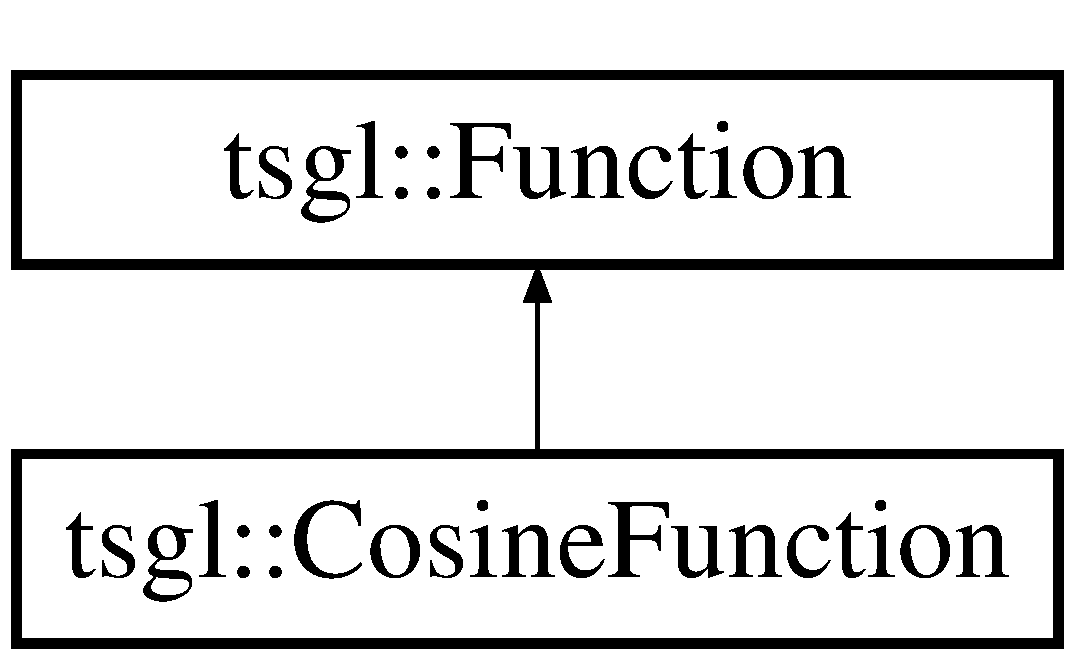
\includegraphics[height=2.000000cm]{classtsgl_1_1_cosine_function}
\end{center}
\end{figure}
\subsection*{Public Member Functions}
\begin{DoxyCompactItemize}
\item 
virtual Decimal \hyperlink{classtsgl_1_1_cosine_function_a69b67c247afe02895d35da9a99bc0ffd}{value\+At} (Decimal x) const 
\begin{DoxyCompactList}\small\item\em Method to determine the value of \hyperlink{classtsgl_1_1_cosine_function}{Cosine\+Function}. \end{DoxyCompactList}\end{DoxyCompactItemize}


\subsection{Detailed Description}
\hyperlink{classtsgl_1_1_function}{Function} to compute the cosine of the input. 

\subsection{Member Function Documentation}
\hypertarget{classtsgl_1_1_cosine_function_a69b67c247afe02895d35da9a99bc0ffd}{}\index{tsgl\+::\+Cosine\+Function@{tsgl\+::\+Cosine\+Function}!value\+At@{value\+At}}
\index{value\+At@{value\+At}!tsgl\+::\+Cosine\+Function@{tsgl\+::\+Cosine\+Function}}
\subsubsection[{value\+At}]{\setlength{\rightskip}{0pt plus 5cm}virtual Decimal tsgl\+::\+Cosine\+Function\+::value\+At (
\begin{DoxyParamCaption}
\item[{Decimal}]{x}
\end{DoxyParamCaption}
) const\hspace{0.3cm}{\ttfamily [inline]}, {\ttfamily [virtual]}}\label{classtsgl_1_1_cosine_function_a69b67c247afe02895d35da9a99bc0ffd}


Method to determine the value of \hyperlink{classtsgl_1_1_cosine_function}{Cosine\+Function}. 

\begin{DoxyReturn}{Returns}
The cosine of {\itshape x}. 
\end{DoxyReturn}


Implements \hyperlink{classtsgl_1_1_function_affb7b3b19a04efefa29a9870d666e912}{tsgl\+::\+Function}.



The documentation for this class was generated from the following file\+:\begin{DoxyCompactItemize}
\item 
Function.\+h\end{DoxyCompactItemize}

\hypertarget{classtsgl_1_1_cube}{}\section{tsgl\+:\+:Cube Class Reference}
\label{classtsgl_1_1_cube}\index{tsgl\+::\+Cube@{tsgl\+::\+Cube}}


Draw an arbitrary \hyperlink{classtsgl_1_1_cube}{Cube} with colored vertices.  




{\ttfamily \#include $<$Cube.\+h$>$}

Inheritance diagram for tsgl\+:\+:Cube\+:\begin{figure}[H]
\begin{center}
\leavevmode
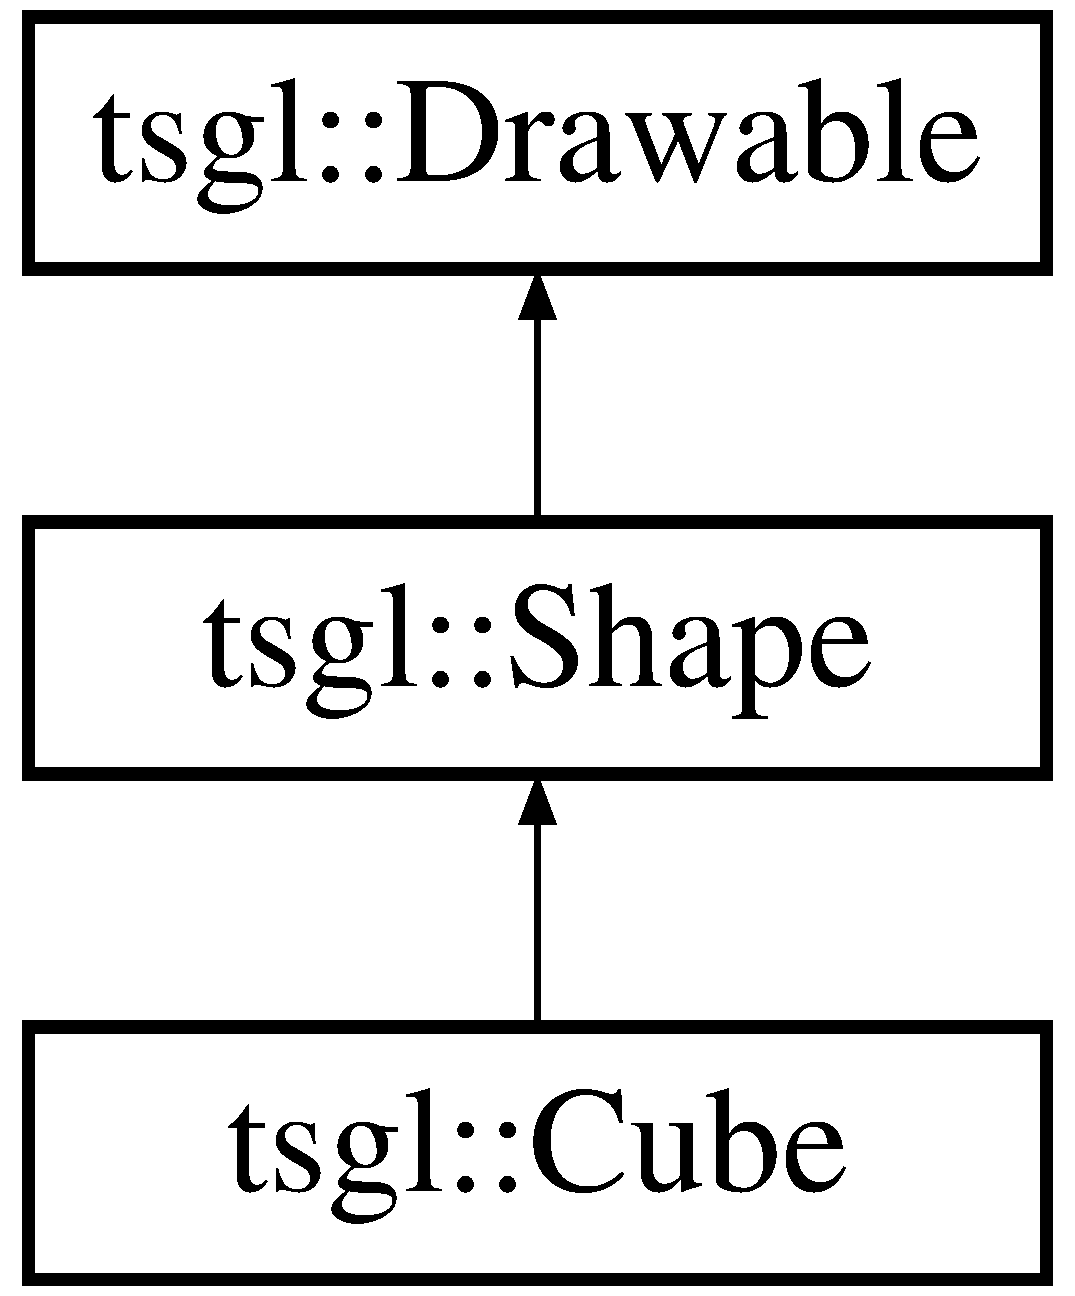
\includegraphics[height=3.000000cm]{classtsgl_1_1_cube}
\end{center}
\end{figure}
\subsection*{Public Member Functions}
\begin{DoxyCompactItemize}
\item 
\hyperlink{classtsgl_1_1_cube_a44a6d1678cd6724d1039b2076e6dcedc}{Cube} (float x, float y, float z, G\+Lfloat side\+Length, float yaw, float pitch, float roll, \hyperlink{structtsgl_1_1_color_float}{Color\+Float} c)
\begin{DoxyCompactList}\small\item\em Explicitly constructs a new \hyperlink{classtsgl_1_1_cube}{Cube}. \end{DoxyCompactList}\item 
\hyperlink{classtsgl_1_1_cube_a19730ea6cdd6888c586f25a168651868}{Cube} (float x, float y, float z, G\+Lfloat side\+Length, float yaw, float pitch, float roll, \hyperlink{structtsgl_1_1_color_float}{Color\+Float} c\mbox{[}$\,$\mbox{]})
\begin{DoxyCompactList}\small\item\em Explicitly constructs a new \hyperlink{classtsgl_1_1_cube}{Cube}. \end{DoxyCompactList}\item 
virtual void \hyperlink{classtsgl_1_1_cube_ae3020b2e435f7c39fae71ea4efcc2f6c}{set\+Side\+Length} (float length)
\begin{DoxyCompactList}\small\item\em Mutates the distance between the \hyperlink{classtsgl_1_1_cube}{Cube}\textquotesingle{}s opposite faces. \end{DoxyCompactList}\item 
virtual void \hyperlink{classtsgl_1_1_cube_a63281031d311a71cf111913f518b66f5}{change\+Side\+Length\+By} (float delta)
\begin{DoxyCompactList}\small\item\em Mutates the distance from the \hyperlink{classtsgl_1_1_cube}{Cube}\textquotesingle{}s front face to its back face by the parameter amount. \end{DoxyCompactList}\item 
virtual G\+Lfloat \hyperlink{classtsgl_1_1_cube_a4dd172e48230f83a70a09e3f3740265d}{get\+Side\+Length} ()
\begin{DoxyCompactList}\small\item\em Accessor for the side length of the \hyperlink{classtsgl_1_1_cube}{Cube}. \end{DoxyCompactList}\item 
virtual void \hyperlink{classtsgl_1_1_cube_a4eb42afdc453fa0c768924a26e5cd870}{set\+Color} (\hyperlink{structtsgl_1_1_color_float}{Color\+Float} c)
\begin{DoxyCompactList}\small\item\em Sets the \hyperlink{classtsgl_1_1_shape}{Shape} to a new color. \end{DoxyCompactList}\item 
virtual void \hyperlink{classtsgl_1_1_cube_a28111319d350040165bd24d92342c7cc}{set\+Color} (\hyperlink{structtsgl_1_1_color_float}{Color\+Float} c\mbox{[}$\,$\mbox{]})
\begin{DoxyCompactList}\small\item\em Sets the \hyperlink{classtsgl_1_1_cube}{Cube} to an array of new colors. \end{DoxyCompactList}\item 
virtual void \hyperlink{classtsgl_1_1_cube_ac1d31d18439024e4160db369df463a7d}{get\+Colors} (std\+::vector$<$ \hyperlink{structtsgl_1_1_color_float}{Color\+Float} $>$ \&color\+Vec)
\begin{DoxyCompactList}\small\item\em Accessor for \hyperlink{classtsgl_1_1_cube}{Cube}\textquotesingle{}s colors. \end{DoxyCompactList}\item 
\mbox{\Hypertarget{classtsgl_1_1_cube_a79c8e76f768ea5cae794c3f856a56280}\label{classtsgl_1_1_cube_a79c8e76f768ea5cae794c3f856a56280}} 
virtual \hyperlink{classtsgl_1_1_cube_a79c8e76f768ea5cae794c3f856a56280}{$\sim$\+Cube} ()
\begin{DoxyCompactList}\small\item\em Destructor for the \hyperlink{classtsgl_1_1_cube}{Cube}. \end{DoxyCompactList}\end{DoxyCompactItemize}
\subsection*{Protected Attributes}
\begin{DoxyCompactItemize}
\item 
\mbox{\Hypertarget{classtsgl_1_1_cube_a1800477d53c864fa2819435285e27669}\label{classtsgl_1_1_cube_a1800477d53c864fa2819435285e27669}} 
G\+Lfloat {\bfseries my\+Side\+Length}
\end{DoxyCompactItemize}
\subsection*{Additional Inherited Members}


\subsection{Detailed Description}
Draw an arbitrary \hyperlink{classtsgl_1_1_cube}{Cube} with colored vertices. 

\hyperlink{classtsgl_1_1_cube}{Cube} is a class for holding vertex data for a \hyperlink{classtsgl_1_1_cube}{Cube}.

\hyperlink{classtsgl_1_1_cube}{Cube} is a 6-\/sided subclass of \hyperlink{classtsgl_1_1_shape}{Shape} with all square faces. 

\subsection{Constructor \& Destructor Documentation}
\mbox{\Hypertarget{classtsgl_1_1_cube_a44a6d1678cd6724d1039b2076e6dcedc}\label{classtsgl_1_1_cube_a44a6d1678cd6724d1039b2076e6dcedc}} 
\index{tsgl\+::\+Cube@{tsgl\+::\+Cube}!Cube@{Cube}}
\index{Cube@{Cube}!tsgl\+::\+Cube@{tsgl\+::\+Cube}}
\subsubsection{\texorpdfstring{Cube()}{Cube()}\hspace{0.1cm}{\footnotesize\ttfamily [1/2]}}
{\footnotesize\ttfamily tsgl\+::\+Cube\+::\+Cube (\begin{DoxyParamCaption}\item[{float}]{x,  }\item[{float}]{y,  }\item[{float}]{z,  }\item[{G\+Lfloat}]{side\+Length,  }\item[{float}]{yaw,  }\item[{float}]{pitch,  }\item[{float}]{roll,  }\item[{\hyperlink{structtsgl_1_1_color_float}{Color\+Float}}]{c }\end{DoxyParamCaption})}



Explicitly constructs a new \hyperlink{classtsgl_1_1_cube}{Cube}. 

Explicit constructor for a \hyperlink{classtsgl_1_1_cube}{Cube} object. 
\begin{DoxyParams}{Parameters}
{\em x} & The x coordinate of the center of the \hyperlink{classtsgl_1_1_cube}{Cube}. \\
\hline
{\em y} & The y coordinate of the center of the \hyperlink{classtsgl_1_1_cube}{Cube}. \\
\hline
{\em z} & The z coordinate of the center of the \hyperlink{classtsgl_1_1_cube}{Cube}. \\
\hline
{\em side\+Length} & The side length of the \hyperlink{classtsgl_1_1_cube}{Cube}. \\
\hline
{\em yaw} & The \hyperlink{classtsgl_1_1_cube}{Cube}\textquotesingle{}s yaw, in degrees. \\
\hline
{\em pitch} & The \hyperlink{classtsgl_1_1_cube}{Cube}\textquotesingle{}s pitch, in degrees. \\
\hline
{\em roll} & The \hyperlink{classtsgl_1_1_cube}{Cube}\textquotesingle{}s roll, in degrees. \\
\hline
{\em c} & A \hyperlink{structtsgl_1_1_color_float}{Color\+Float} for the \hyperlink{classtsgl_1_1_cube}{Cube}\textquotesingle{}s vertex colors. \\
\hline
\end{DoxyParams}
\begin{DoxyWarning}{Warning}
An invariant is held where if length, width, or height isn\textquotesingle{}t positive then an error message is given. 
\end{DoxyWarning}
\begin{DoxyReturn}{Returns}
A new \hyperlink{classtsgl_1_1_cube}{Cube} with a buffer for storing the specified numbered of vertices. 
\end{DoxyReturn}
\mbox{\Hypertarget{classtsgl_1_1_cube_a19730ea6cdd6888c586f25a168651868}\label{classtsgl_1_1_cube_a19730ea6cdd6888c586f25a168651868}} 
\index{tsgl\+::\+Cube@{tsgl\+::\+Cube}!Cube@{Cube}}
\index{Cube@{Cube}!tsgl\+::\+Cube@{tsgl\+::\+Cube}}
\subsubsection{\texorpdfstring{Cube()}{Cube()}\hspace{0.1cm}{\footnotesize\ttfamily [2/2]}}
{\footnotesize\ttfamily tsgl\+::\+Cube\+::\+Cube (\begin{DoxyParamCaption}\item[{float}]{x,  }\item[{float}]{y,  }\item[{float}]{z,  }\item[{G\+Lfloat}]{side\+Length,  }\item[{float}]{yaw,  }\item[{float}]{pitch,  }\item[{float}]{roll,  }\item[{\hyperlink{structtsgl_1_1_color_float}{Color\+Float}}]{c\mbox{[}$\,$\mbox{]} }\end{DoxyParamCaption})}



Explicitly constructs a new \hyperlink{classtsgl_1_1_cube}{Cube}. 

Explicit constructor for a \hyperlink{classtsgl_1_1_cube}{Cube} object. 
\begin{DoxyParams}{Parameters}
{\em x} & The x coordinate of the center of the \hyperlink{classtsgl_1_1_cube}{Cube}. \\
\hline
{\em y} & The y coordinate of the center of the \hyperlink{classtsgl_1_1_cube}{Cube}. \\
\hline
{\em z} & The z coordinate of the center of the \hyperlink{classtsgl_1_1_cube}{Cube}. \\
\hline
{\em side\+Length} & The side length of the \hyperlink{classtsgl_1_1_cube}{Cube}. \\
\hline
{\em yaw} & The \hyperlink{classtsgl_1_1_cube}{Cube}\textquotesingle{}s yaw, in degrees. \\
\hline
{\em pitch} & The \hyperlink{classtsgl_1_1_cube}{Cube}\textquotesingle{}s pitch, in degrees. \\
\hline
{\em roll} & The \hyperlink{classtsgl_1_1_cube}{Cube}\textquotesingle{}s roll, in degrees. \\
\hline
{\em c} & An array of Color\+Floats for the \hyperlink{classtsgl_1_1_cube}{Cube}\textquotesingle{}s vertex colors. \\
\hline
\end{DoxyParams}
\begin{DoxyWarning}{Warning}
An invariant is held where if length, width, or height isn\textquotesingle{}t positive then an error message is given. 
\end{DoxyWarning}
\begin{DoxyReturn}{Returns}
A new \hyperlink{classtsgl_1_1_cube}{Cube} with a buffer for storing the specified numbered of vertices. 
\end{DoxyReturn}


\subsection{Member Function Documentation}
\mbox{\Hypertarget{classtsgl_1_1_cube_a63281031d311a71cf111913f518b66f5}\label{classtsgl_1_1_cube_a63281031d311a71cf111913f518b66f5}} 
\index{tsgl\+::\+Cube@{tsgl\+::\+Cube}!change\+Side\+Length\+By@{change\+Side\+Length\+By}}
\index{change\+Side\+Length\+By@{change\+Side\+Length\+By}!tsgl\+::\+Cube@{tsgl\+::\+Cube}}
\subsubsection{\texorpdfstring{change\+Side\+Length\+By()}{changeSideLengthBy()}}
{\footnotesize\ttfamily void tsgl\+::\+Cube\+::change\+Side\+Length\+By (\begin{DoxyParamCaption}\item[{float}]{delta }\end{DoxyParamCaption})\hspace{0.3cm}{\ttfamily [virtual]}}



Mutates the distance from the \hyperlink{classtsgl_1_1_cube}{Cube}\textquotesingle{}s front face to its back face by the parameter amount. 


\begin{DoxyParams}{Parameters}
{\em delta} & The amount by which to change the length of the \hyperlink{classtsgl_1_1_cube}{Cube}. \\
\hline
\end{DoxyParams}
\mbox{\Hypertarget{classtsgl_1_1_cube_ac1d31d18439024e4160db369df463a7d}\label{classtsgl_1_1_cube_ac1d31d18439024e4160db369df463a7d}} 
\index{tsgl\+::\+Cube@{tsgl\+::\+Cube}!get\+Colors@{get\+Colors}}
\index{get\+Colors@{get\+Colors}!tsgl\+::\+Cube@{tsgl\+::\+Cube}}
\subsubsection{\texorpdfstring{get\+Colors()}{getColors()}}
{\footnotesize\ttfamily void tsgl\+::\+Cube\+::get\+Colors (\begin{DoxyParamCaption}\item[{std\+::vector$<$ \hyperlink{structtsgl_1_1_color_float}{Color\+Float} $>$ \&}]{color\+Vec }\end{DoxyParamCaption})\hspace{0.3cm}{\ttfamily [virtual]}}



Accessor for \hyperlink{classtsgl_1_1_cube}{Cube}\textquotesingle{}s colors. 

Populates the reference parameter vector with a \hyperlink{structtsgl_1_1_color_float}{Color\+Float} for each corner of \hyperlink{classtsgl_1_1_cube}{Cube}. 
\begin{DoxyParams}{Parameters}
{\em color\+Vec} & A vector of Color\+Floats to which the Color\+Floats associated with \hyperlink{classtsgl_1_1_cube}{Cube} will be pushed. \\
\hline
\end{DoxyParams}
\begin{DoxyNote}{Note}
Overrides \hyperlink{classtsgl_1_1_shape_a6f54fe4d049f69a287edf8335a9509f8}{Shape\+::get\+Colors()}. 
\end{DoxyNote}


Reimplemented from \hyperlink{classtsgl_1_1_shape_a6f54fe4d049f69a287edf8335a9509f8}{tsgl\+::\+Shape}.



Referenced by set\+Color().

\mbox{\Hypertarget{classtsgl_1_1_cube_a4dd172e48230f83a70a09e3f3740265d}\label{classtsgl_1_1_cube_a4dd172e48230f83a70a09e3f3740265d}} 
\index{tsgl\+::\+Cube@{tsgl\+::\+Cube}!get\+Side\+Length@{get\+Side\+Length}}
\index{get\+Side\+Length@{get\+Side\+Length}!tsgl\+::\+Cube@{tsgl\+::\+Cube}}
\subsubsection{\texorpdfstring{get\+Side\+Length()}{getSideLength()}}
{\footnotesize\ttfamily virtual G\+Lfloat tsgl\+::\+Cube\+::get\+Side\+Length (\begin{DoxyParamCaption}{ }\end{DoxyParamCaption})\hspace{0.3cm}{\ttfamily [inline]}, {\ttfamily [virtual]}}



Accessor for the side length of the \hyperlink{classtsgl_1_1_cube}{Cube}. 

Returns the value of the my\+Side\+Length private variable, a G\+Lfloat. \mbox{\Hypertarget{classtsgl_1_1_cube_a4eb42afdc453fa0c768924a26e5cd870}\label{classtsgl_1_1_cube_a4eb42afdc453fa0c768924a26e5cd870}} 
\index{tsgl\+::\+Cube@{tsgl\+::\+Cube}!set\+Color@{set\+Color}}
\index{set\+Color@{set\+Color}!tsgl\+::\+Cube@{tsgl\+::\+Cube}}
\subsubsection{\texorpdfstring{set\+Color()}{setColor()}\hspace{0.1cm}{\footnotesize\ttfamily [1/2]}}
{\footnotesize\ttfamily virtual void tsgl\+::\+Cube\+::set\+Color (\begin{DoxyParamCaption}\item[{\hyperlink{structtsgl_1_1_color_float}{Color\+Float}}]{c }\end{DoxyParamCaption})\hspace{0.3cm}{\ttfamily [inline]}, {\ttfamily [virtual]}}



Sets the \hyperlink{classtsgl_1_1_shape}{Shape} to a new color. 


\begin{DoxyParams}{Parameters}
{\em c} & The new \hyperlink{structtsgl_1_1_color_float}{Color\+Float}. \\
\hline
\end{DoxyParams}


Reimplemented from \hyperlink{classtsgl_1_1_shape_abdb01321cddfd2db1481eefbc2836f70}{tsgl\+::\+Shape}.

\mbox{\Hypertarget{classtsgl_1_1_cube_a28111319d350040165bd24d92342c7cc}\label{classtsgl_1_1_cube_a28111319d350040165bd24d92342c7cc}} 
\index{tsgl\+::\+Cube@{tsgl\+::\+Cube}!set\+Color@{set\+Color}}
\index{set\+Color@{set\+Color}!tsgl\+::\+Cube@{tsgl\+::\+Cube}}
\subsubsection{\texorpdfstring{set\+Color()}{setColor()}\hspace{0.1cm}{\footnotesize\ttfamily [2/2]}}
{\footnotesize\ttfamily void tsgl\+::\+Cube\+::set\+Color (\begin{DoxyParamCaption}\item[{\hyperlink{structtsgl_1_1_color_float}{Color\+Float}}]{c\mbox{[}$\,$\mbox{]} }\end{DoxyParamCaption})\hspace{0.3cm}{\ttfamily [virtual]}}



Sets the \hyperlink{classtsgl_1_1_cube}{Cube} to an array of new colors. 


\begin{DoxyParams}{Parameters}
{\em c} & An array of new Color\+Floats.\\
\hline
\end{DoxyParams}
The array should have 8 Color\+Floats minimum, one for each corner. 

Reimplemented from \hyperlink{classtsgl_1_1_shape_ad7e554b5d4cea111ec518548b9f21388}{tsgl\+::\+Shape}.

\mbox{\Hypertarget{classtsgl_1_1_cube_ae3020b2e435f7c39fae71ea4efcc2f6c}\label{classtsgl_1_1_cube_ae3020b2e435f7c39fae71ea4efcc2f6c}} 
\index{tsgl\+::\+Cube@{tsgl\+::\+Cube}!set\+Side\+Length@{set\+Side\+Length}}
\index{set\+Side\+Length@{set\+Side\+Length}!tsgl\+::\+Cube@{tsgl\+::\+Cube}}
\subsubsection{\texorpdfstring{set\+Side\+Length()}{setSideLength()}}
{\footnotesize\ttfamily void tsgl\+::\+Cube\+::set\+Side\+Length (\begin{DoxyParamCaption}\item[{float}]{length }\end{DoxyParamCaption})\hspace{0.3cm}{\ttfamily [virtual]}}



Mutates the distance between the \hyperlink{classtsgl_1_1_cube}{Cube}\textquotesingle{}s opposite faces. 


\begin{DoxyParams}{Parameters}
{\em length} & The \hyperlink{classtsgl_1_1_cube}{Cube}\textquotesingle{}s new side length. \\
\hline
\end{DoxyParams}


The documentation for this class was generated from the following files\+:\begin{DoxyCompactItemize}
\item 
Cube.\+h\item 
Cube.\+cpp\end{DoxyCompactItemize}

\hypertarget{classtsgl_1_1_cuboid}{}\section{tsgl\+:\+:Cuboid Class Reference}
\label{classtsgl_1_1_cuboid}\index{tsgl\+::\+Cuboid@{tsgl\+::\+Cuboid}}


Draw an arbitrary \hyperlink{classtsgl_1_1_cuboid}{Cuboid} with colored vertices.  




{\ttfamily \#include $<$Cuboid.\+h$>$}

Inheritance diagram for tsgl\+:\+:Cuboid\+:\begin{figure}[H]
\begin{center}
\leavevmode
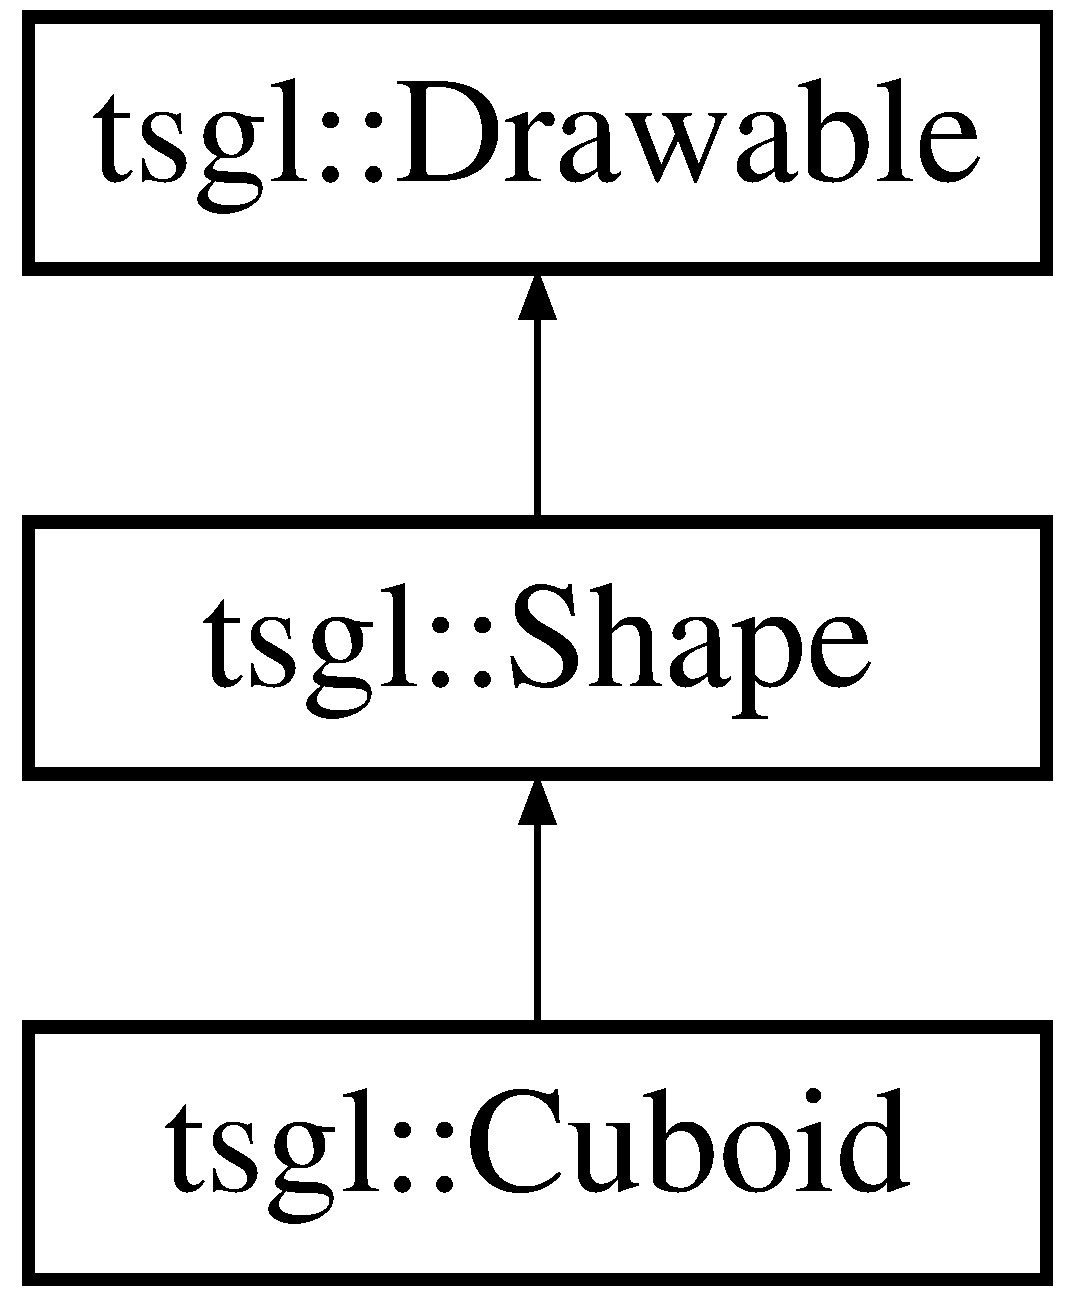
\includegraphics[height=3.000000cm]{classtsgl_1_1_cuboid}
\end{center}
\end{figure}
\subsection*{Public Member Functions}
\begin{DoxyCompactItemize}
\item 
\hyperlink{classtsgl_1_1_cuboid_ac6fae2d4edcb10ea1478c840012f5c2a}{Cuboid} (float x, float y, float z, G\+Lfloat width, G\+Lfloat height, G\+Lfloat length, float yaw, float pitch, float roll, \hyperlink{structtsgl_1_1_color_float}{Color\+Float} c)
\begin{DoxyCompactList}\small\item\em Explicitly constructs a new \hyperlink{classtsgl_1_1_cuboid}{Cuboid}. \end{DoxyCompactList}\item 
\hyperlink{classtsgl_1_1_cuboid_aeae9324a13708f6e00d4423bd3ebba86}{Cuboid} (float x, float y, float z, G\+Lfloat width, G\+Lfloat height, G\+Lfloat length, float yaw, float pitch, float roll, \hyperlink{structtsgl_1_1_color_float}{Color\+Float} c\mbox{[}$\,$\mbox{]})
\begin{DoxyCompactList}\small\item\em Explicitly constructs a new \hyperlink{classtsgl_1_1_cuboid}{Cuboid}. \end{DoxyCompactList}\item 
virtual void \hyperlink{classtsgl_1_1_cuboid_a877809edb072286dd3157714fc2e405d}{set\+Length} (G\+Lfloat length)
\begin{DoxyCompactList}\small\item\em Mutates the distance from the \hyperlink{classtsgl_1_1_cuboid}{Cuboid}\textquotesingle{}s front face to its back face. \end{DoxyCompactList}\item 
virtual void \hyperlink{classtsgl_1_1_cuboid_ac8b9e098acd3b46dafae304f1288aa3d}{change\+Length\+By} (G\+Lfloat delta)
\begin{DoxyCompactList}\small\item\em Mutates the distance from the \hyperlink{classtsgl_1_1_cuboid}{Cuboid}\textquotesingle{}s front face to its back face by the parameter amount. \end{DoxyCompactList}\item 
virtual void \hyperlink{classtsgl_1_1_cuboid_a1bb873bf2fb9a51996219e5c6b013520}{set\+Width} (G\+Lfloat width)
\begin{DoxyCompactList}\small\item\em Mutates the distance from the \hyperlink{classtsgl_1_1_cuboid}{Cuboid}\textquotesingle{}s left face to its right face. \end{DoxyCompactList}\item 
virtual void \hyperlink{classtsgl_1_1_cuboid_a72470bd9e57eb12440883ff69b5a9bc4}{change\+Width\+By} (G\+Lfloat delta)
\begin{DoxyCompactList}\small\item\em Mutates the distance from the \hyperlink{classtsgl_1_1_cuboid}{Cuboid}\textquotesingle{}s left face to its right face by the parameter amount. \end{DoxyCompactList}\item 
virtual void \hyperlink{classtsgl_1_1_cuboid_a662cfb3fdb5afb9dff0b7efe517c8641}{set\+Height} (G\+Lfloat height)
\begin{DoxyCompactList}\small\item\em Mutates the distance from the center of the \hyperlink{classtsgl_1_1_cuboid}{Cuboid}\textquotesingle{}s base to the top. \end{DoxyCompactList}\item 
virtual void \hyperlink{classtsgl_1_1_cuboid_af3c9270b597b8e2ff2d16929c81c3db3}{change\+Height\+By} (G\+Lfloat delta)
\begin{DoxyCompactList}\small\item\em Mutates the distance from the center of the \hyperlink{classtsgl_1_1_cuboid}{Cuboid}\textquotesingle{}s base to the top by the parameter amount. \end{DoxyCompactList}\item 
virtual G\+Lfloat \hyperlink{classtsgl_1_1_cuboid_ae7780009759998eb7763d9f885e8e2b8}{get\+Length} ()
\begin{DoxyCompactList}\small\item\em Accessor for the length of the \hyperlink{classtsgl_1_1_prism}{Prism}. \end{DoxyCompactList}\item 
virtual G\+Lfloat \hyperlink{classtsgl_1_1_cuboid_a4703e0321f31b4757673c8faf7b2b8df}{get\+Height} ()
\begin{DoxyCompactList}\small\item\em Accessor for the height of the \hyperlink{classtsgl_1_1_prism}{Prism}. \end{DoxyCompactList}\item 
virtual G\+Lfloat \hyperlink{classtsgl_1_1_cuboid_a6f5084919851fa715c931b8382a34d6c}{get\+Width} ()
\begin{DoxyCompactList}\small\item\em Accessor for the width of the \hyperlink{classtsgl_1_1_prism}{Prism}. \end{DoxyCompactList}\item 
virtual void \hyperlink{classtsgl_1_1_cuboid_a683f0eeb463e9779e954955f92f12f8e}{set\+Color} (\hyperlink{structtsgl_1_1_color_float}{Color\+Float} c)
\begin{DoxyCompactList}\small\item\em Sets the \hyperlink{classtsgl_1_1_shape}{Shape} to a new color. \end{DoxyCompactList}\item 
virtual void \hyperlink{classtsgl_1_1_cuboid_aab8a70aff0dcede030ac51277c0dc255}{set\+Color} (\hyperlink{structtsgl_1_1_color_float}{Color\+Float} c\mbox{[}$\,$\mbox{]})
\begin{DoxyCompactList}\small\item\em Sets the \hyperlink{classtsgl_1_1_cuboid}{Cuboid} to an array of new colors. \end{DoxyCompactList}\item 
virtual void \hyperlink{classtsgl_1_1_cuboid_ac3e7d161cb2dbb02cf000e92d84e10ba}{get\+Colors} (std\+::vector$<$ \hyperlink{structtsgl_1_1_color_float}{Color\+Float} $>$ \&color\+Vec)
\begin{DoxyCompactList}\small\item\em Accessor for \hyperlink{classtsgl_1_1_cuboid}{Cuboid}\textquotesingle{}s colors. \end{DoxyCompactList}\end{DoxyCompactItemize}
\subsection*{Protected Attributes}
\begin{DoxyCompactItemize}
\item 
\mbox{\Hypertarget{classtsgl_1_1_cuboid_ac20cb617d0f65a63ca51e1088f36e6bb}\label{classtsgl_1_1_cuboid_ac20cb617d0f65a63ca51e1088f36e6bb}} 
G\+Lfloat {\bfseries my\+Length}
\item 
\mbox{\Hypertarget{classtsgl_1_1_cuboid_a1e910718e6b411d49f6da3ecdc77c865}\label{classtsgl_1_1_cuboid_a1e910718e6b411d49f6da3ecdc77c865}} 
G\+Lfloat {\bfseries my\+Width}
\item 
\mbox{\Hypertarget{classtsgl_1_1_cuboid_affe9afb7d35302a866db56a8d4c190cd}\label{classtsgl_1_1_cuboid_affe9afb7d35302a866db56a8d4c190cd}} 
G\+Lfloat {\bfseries my\+Height}
\end{DoxyCompactItemize}
\subsection*{Additional Inherited Members}


\subsection{Detailed Description}
Draw an arbitrary \hyperlink{classtsgl_1_1_cuboid}{Cuboid} with colored vertices. 

\hyperlink{classtsgl_1_1_cuboid}{Cuboid} is a class for holding vertex data for a \hyperlink{classtsgl_1_1_cuboid}{Cuboid}.

\hyperlink{classtsgl_1_1_cuboid}{Cuboid} is a 6-\/sided subclass of \hyperlink{classtsgl_1_1_shape}{Shape} with all rectangular faces. 

\subsection{Constructor \& Destructor Documentation}
\mbox{\Hypertarget{classtsgl_1_1_cuboid_ac6fae2d4edcb10ea1478c840012f5c2a}\label{classtsgl_1_1_cuboid_ac6fae2d4edcb10ea1478c840012f5c2a}} 
\index{tsgl\+::\+Cuboid@{tsgl\+::\+Cuboid}!Cuboid@{Cuboid}}
\index{Cuboid@{Cuboid}!tsgl\+::\+Cuboid@{tsgl\+::\+Cuboid}}
\subsubsection{\texorpdfstring{Cuboid()}{Cuboid()}\hspace{0.1cm}{\footnotesize\ttfamily [1/2]}}
{\footnotesize\ttfamily tsgl\+::\+Cuboid\+::\+Cuboid (\begin{DoxyParamCaption}\item[{float}]{x,  }\item[{float}]{y,  }\item[{float}]{z,  }\item[{G\+Lfloat}]{width,  }\item[{G\+Lfloat}]{height,  }\item[{G\+Lfloat}]{length,  }\item[{float}]{yaw,  }\item[{float}]{pitch,  }\item[{float}]{roll,  }\item[{\hyperlink{structtsgl_1_1_color_float}{Color\+Float}}]{c }\end{DoxyParamCaption})}



Explicitly constructs a new \hyperlink{classtsgl_1_1_cuboid}{Cuboid}. 

Explicit constructor for a \hyperlink{classtsgl_1_1_cuboid}{Cuboid} object. 
\begin{DoxyParams}{Parameters}
{\em x} & The x coordinate of the center of the \hyperlink{classtsgl_1_1_cuboid}{Cuboid}. \\
\hline
{\em y} & The y coordinate of the center of the \hyperlink{classtsgl_1_1_cuboid}{Cuboid}. \\
\hline
{\em z} & The z coordinate of the center of the \hyperlink{classtsgl_1_1_cuboid}{Cuboid}. \\
\hline
{\em length} & The length of the \hyperlink{classtsgl_1_1_cuboid}{Cuboid}. \\
\hline
{\em width} & The width of the \hyperlink{classtsgl_1_1_cuboid}{Cuboid}. \\
\hline
{\em height} & The height of the \hyperlink{classtsgl_1_1_cuboid}{Cuboid}. \\
\hline
{\em yaw} & The \hyperlink{classtsgl_1_1_cuboid}{Cuboid}\textquotesingle{}s yaw. \\
\hline
{\em pitch} & The \hyperlink{classtsgl_1_1_cuboid}{Cuboid}\textquotesingle{}s pitch. \\
\hline
{\em roll} & The \hyperlink{classtsgl_1_1_cuboid}{Cuboid}\textquotesingle{}s roll. \\
\hline
{\em c} & A \hyperlink{structtsgl_1_1_color_float}{Color\+Float} for the \hyperlink{classtsgl_1_1_cuboid}{Cuboid}\textquotesingle{}s vertex colors. \\
\hline
\end{DoxyParams}
\begin{DoxyWarning}{Warning}
An invariant is held where if length, width, or height isn\textquotesingle{}t positive then an error message is given. 
\end{DoxyWarning}
\begin{DoxyReturn}{Returns}
A new \hyperlink{classtsgl_1_1_cuboid}{Cuboid} with a buffer for storing the specified numbered of vertices. 
\end{DoxyReturn}
\mbox{\Hypertarget{classtsgl_1_1_cuboid_aeae9324a13708f6e00d4423bd3ebba86}\label{classtsgl_1_1_cuboid_aeae9324a13708f6e00d4423bd3ebba86}} 
\index{tsgl\+::\+Cuboid@{tsgl\+::\+Cuboid}!Cuboid@{Cuboid}}
\index{Cuboid@{Cuboid}!tsgl\+::\+Cuboid@{tsgl\+::\+Cuboid}}
\subsubsection{\texorpdfstring{Cuboid()}{Cuboid()}\hspace{0.1cm}{\footnotesize\ttfamily [2/2]}}
{\footnotesize\ttfamily tsgl\+::\+Cuboid\+::\+Cuboid (\begin{DoxyParamCaption}\item[{float}]{x,  }\item[{float}]{y,  }\item[{float}]{z,  }\item[{G\+Lfloat}]{width,  }\item[{G\+Lfloat}]{height,  }\item[{G\+Lfloat}]{length,  }\item[{float}]{yaw,  }\item[{float}]{pitch,  }\item[{float}]{roll,  }\item[{\hyperlink{structtsgl_1_1_color_float}{Color\+Float}}]{c\mbox{[}$\,$\mbox{]} }\end{DoxyParamCaption})}



Explicitly constructs a new \hyperlink{classtsgl_1_1_cuboid}{Cuboid}. 

Explicit constructor for a \hyperlink{classtsgl_1_1_cuboid}{Cuboid} object. 
\begin{DoxyParams}{Parameters}
{\em x} & The x coordinate of the center of the \hyperlink{classtsgl_1_1_cuboid}{Cuboid}. \\
\hline
{\em y} & The y coordinate of the center of the \hyperlink{classtsgl_1_1_cuboid}{Cuboid}. \\
\hline
{\em z} & The z coordinate of the center of the \hyperlink{classtsgl_1_1_cuboid}{Cuboid}. \\
\hline
{\em length} & The length of the \hyperlink{classtsgl_1_1_cuboid}{Cuboid}. \\
\hline
{\em width} & The width of the \hyperlink{classtsgl_1_1_cuboid}{Cuboid}. \\
\hline
{\em height} & The height of the \hyperlink{classtsgl_1_1_cuboid}{Cuboid}. \\
\hline
{\em yaw} & The \hyperlink{classtsgl_1_1_cuboid}{Cuboid}\textquotesingle{}s yaw. \\
\hline
{\em pitch} & The \hyperlink{classtsgl_1_1_cuboid}{Cuboid}\textquotesingle{}s pitch. \\
\hline
{\em roll} & The \hyperlink{classtsgl_1_1_cuboid}{Cuboid}\textquotesingle{}s roll. \\
\hline
{\em c} & An array of Color\+Floats for the \hyperlink{classtsgl_1_1_cuboid}{Cuboid}\textquotesingle{}s vertex colors. \\
\hline
\end{DoxyParams}
\begin{DoxyWarning}{Warning}
An invariant is held where if length, width, or height isn\textquotesingle{}t positive then an error message is given. 
\end{DoxyWarning}
\begin{DoxyReturn}{Returns}
A new \hyperlink{classtsgl_1_1_cuboid}{Cuboid} with a buffer for storing the specified numbered of vertices. 
\end{DoxyReturn}


\subsection{Member Function Documentation}
\mbox{\Hypertarget{classtsgl_1_1_cuboid_af3c9270b597b8e2ff2d16929c81c3db3}\label{classtsgl_1_1_cuboid_af3c9270b597b8e2ff2d16929c81c3db3}} 
\index{tsgl\+::\+Cuboid@{tsgl\+::\+Cuboid}!change\+Height\+By@{change\+Height\+By}}
\index{change\+Height\+By@{change\+Height\+By}!tsgl\+::\+Cuboid@{tsgl\+::\+Cuboid}}
\subsubsection{\texorpdfstring{change\+Height\+By()}{changeHeightBy()}}
{\footnotesize\ttfamily void tsgl\+::\+Cuboid\+::change\+Height\+By (\begin{DoxyParamCaption}\item[{G\+Lfloat}]{delta }\end{DoxyParamCaption})\hspace{0.3cm}{\ttfamily [virtual]}}



Mutates the distance from the center of the \hyperlink{classtsgl_1_1_cuboid}{Cuboid}\textquotesingle{}s base to the top by the parameter amount. 


\begin{DoxyParams}{Parameters}
{\em delta} & The amount by which to change the height of the \hyperlink{classtsgl_1_1_cuboid}{Cuboid}. \\
\hline
\end{DoxyParams}
\mbox{\Hypertarget{classtsgl_1_1_cuboid_ac8b9e098acd3b46dafae304f1288aa3d}\label{classtsgl_1_1_cuboid_ac8b9e098acd3b46dafae304f1288aa3d}} 
\index{tsgl\+::\+Cuboid@{tsgl\+::\+Cuboid}!change\+Length\+By@{change\+Length\+By}}
\index{change\+Length\+By@{change\+Length\+By}!tsgl\+::\+Cuboid@{tsgl\+::\+Cuboid}}
\subsubsection{\texorpdfstring{change\+Length\+By()}{changeLengthBy()}}
{\footnotesize\ttfamily void tsgl\+::\+Cuboid\+::change\+Length\+By (\begin{DoxyParamCaption}\item[{G\+Lfloat}]{delta }\end{DoxyParamCaption})\hspace{0.3cm}{\ttfamily [virtual]}}



Mutates the distance from the \hyperlink{classtsgl_1_1_cuboid}{Cuboid}\textquotesingle{}s front face to its back face by the parameter amount. 


\begin{DoxyParams}{Parameters}
{\em delta} & The amount by which to change the length of the \hyperlink{classtsgl_1_1_cuboid}{Cuboid}. \\
\hline
\end{DoxyParams}
\mbox{\Hypertarget{classtsgl_1_1_cuboid_a72470bd9e57eb12440883ff69b5a9bc4}\label{classtsgl_1_1_cuboid_a72470bd9e57eb12440883ff69b5a9bc4}} 
\index{tsgl\+::\+Cuboid@{tsgl\+::\+Cuboid}!change\+Width\+By@{change\+Width\+By}}
\index{change\+Width\+By@{change\+Width\+By}!tsgl\+::\+Cuboid@{tsgl\+::\+Cuboid}}
\subsubsection{\texorpdfstring{change\+Width\+By()}{changeWidthBy()}}
{\footnotesize\ttfamily void tsgl\+::\+Cuboid\+::change\+Width\+By (\begin{DoxyParamCaption}\item[{G\+Lfloat}]{delta }\end{DoxyParamCaption})\hspace{0.3cm}{\ttfamily [virtual]}}



Mutates the distance from the \hyperlink{classtsgl_1_1_cuboid}{Cuboid}\textquotesingle{}s left face to its right face by the parameter amount. 


\begin{DoxyParams}{Parameters}
{\em delta} & The amount by which to change the width of the \hyperlink{classtsgl_1_1_cuboid}{Cuboid}. \\
\hline
\end{DoxyParams}
\mbox{\Hypertarget{classtsgl_1_1_cuboid_ac3e7d161cb2dbb02cf000e92d84e10ba}\label{classtsgl_1_1_cuboid_ac3e7d161cb2dbb02cf000e92d84e10ba}} 
\index{tsgl\+::\+Cuboid@{tsgl\+::\+Cuboid}!get\+Colors@{get\+Colors}}
\index{get\+Colors@{get\+Colors}!tsgl\+::\+Cuboid@{tsgl\+::\+Cuboid}}
\subsubsection{\texorpdfstring{get\+Colors()}{getColors()}}
{\footnotesize\ttfamily void tsgl\+::\+Cuboid\+::get\+Colors (\begin{DoxyParamCaption}\item[{std\+::vector$<$ \hyperlink{structtsgl_1_1_color_float}{Color\+Float} $>$ \&}]{color\+Vec }\end{DoxyParamCaption})\hspace{0.3cm}{\ttfamily [virtual]}}



Accessor for \hyperlink{classtsgl_1_1_cuboid}{Cuboid}\textquotesingle{}s colors. 

Populates the reference parameter vector with a \hyperlink{structtsgl_1_1_color_float}{Color\+Float} for each corner of \hyperlink{classtsgl_1_1_cuboid}{Cuboid}. 
\begin{DoxyParams}{Parameters}
{\em color\+Vec} & A vector of Color\+Floats to which the Color\+Floats associated with \hyperlink{classtsgl_1_1_cuboid}{Cuboid} will be pushed. \\
\hline
\end{DoxyParams}
\begin{DoxyNote}{Note}
Overrides \hyperlink{classtsgl_1_1_shape_a6f54fe4d049f69a287edf8335a9509f8}{Shape\+::get\+Colors()}. 
\end{DoxyNote}


Reimplemented from \hyperlink{classtsgl_1_1_shape_a6f54fe4d049f69a287edf8335a9509f8}{tsgl\+::\+Shape}.



Referenced by set\+Color().

\mbox{\Hypertarget{classtsgl_1_1_cuboid_a4703e0321f31b4757673c8faf7b2b8df}\label{classtsgl_1_1_cuboid_a4703e0321f31b4757673c8faf7b2b8df}} 
\index{tsgl\+::\+Cuboid@{tsgl\+::\+Cuboid}!get\+Height@{get\+Height}}
\index{get\+Height@{get\+Height}!tsgl\+::\+Cuboid@{tsgl\+::\+Cuboid}}
\subsubsection{\texorpdfstring{get\+Height()}{getHeight()}}
{\footnotesize\ttfamily virtual G\+Lfloat tsgl\+::\+Cuboid\+::get\+Height (\begin{DoxyParamCaption}{ }\end{DoxyParamCaption})\hspace{0.3cm}{\ttfamily [inline]}, {\ttfamily [virtual]}}



Accessor for the height of the \hyperlink{classtsgl_1_1_prism}{Prism}. 

Returns the value of the my\+Height private variable, a G\+Lfloat. \mbox{\Hypertarget{classtsgl_1_1_cuboid_ae7780009759998eb7763d9f885e8e2b8}\label{classtsgl_1_1_cuboid_ae7780009759998eb7763d9f885e8e2b8}} 
\index{tsgl\+::\+Cuboid@{tsgl\+::\+Cuboid}!get\+Length@{get\+Length}}
\index{get\+Length@{get\+Length}!tsgl\+::\+Cuboid@{tsgl\+::\+Cuboid}}
\subsubsection{\texorpdfstring{get\+Length()}{getLength()}}
{\footnotesize\ttfamily virtual G\+Lfloat tsgl\+::\+Cuboid\+::get\+Length (\begin{DoxyParamCaption}{ }\end{DoxyParamCaption})\hspace{0.3cm}{\ttfamily [inline]}, {\ttfamily [virtual]}}



Accessor for the length of the \hyperlink{classtsgl_1_1_prism}{Prism}. 

Returns the value of the my\+Length private variable, a G\+Lfloat. \mbox{\Hypertarget{classtsgl_1_1_cuboid_a6f5084919851fa715c931b8382a34d6c}\label{classtsgl_1_1_cuboid_a6f5084919851fa715c931b8382a34d6c}} 
\index{tsgl\+::\+Cuboid@{tsgl\+::\+Cuboid}!get\+Width@{get\+Width}}
\index{get\+Width@{get\+Width}!tsgl\+::\+Cuboid@{tsgl\+::\+Cuboid}}
\subsubsection{\texorpdfstring{get\+Width()}{getWidth()}}
{\footnotesize\ttfamily virtual G\+Lfloat tsgl\+::\+Cuboid\+::get\+Width (\begin{DoxyParamCaption}{ }\end{DoxyParamCaption})\hspace{0.3cm}{\ttfamily [inline]}, {\ttfamily [virtual]}}



Accessor for the width of the \hyperlink{classtsgl_1_1_prism}{Prism}. 

Returns the value of the my\+Width private variable, a G\+Lfloat. \mbox{\Hypertarget{classtsgl_1_1_cuboid_a683f0eeb463e9779e954955f92f12f8e}\label{classtsgl_1_1_cuboid_a683f0eeb463e9779e954955f92f12f8e}} 
\index{tsgl\+::\+Cuboid@{tsgl\+::\+Cuboid}!set\+Color@{set\+Color}}
\index{set\+Color@{set\+Color}!tsgl\+::\+Cuboid@{tsgl\+::\+Cuboid}}
\subsubsection{\texorpdfstring{set\+Color()}{setColor()}\hspace{0.1cm}{\footnotesize\ttfamily [1/2]}}
{\footnotesize\ttfamily virtual void tsgl\+::\+Cuboid\+::set\+Color (\begin{DoxyParamCaption}\item[{\hyperlink{structtsgl_1_1_color_float}{Color\+Float}}]{c }\end{DoxyParamCaption})\hspace{0.3cm}{\ttfamily [inline]}, {\ttfamily [virtual]}}



Sets the \hyperlink{classtsgl_1_1_shape}{Shape} to a new color. 


\begin{DoxyParams}{Parameters}
{\em c} & The new \hyperlink{structtsgl_1_1_color_float}{Color\+Float}. \\
\hline
\end{DoxyParams}


Reimplemented from \hyperlink{classtsgl_1_1_shape_abdb01321cddfd2db1481eefbc2836f70}{tsgl\+::\+Shape}.

\mbox{\Hypertarget{classtsgl_1_1_cuboid_aab8a70aff0dcede030ac51277c0dc255}\label{classtsgl_1_1_cuboid_aab8a70aff0dcede030ac51277c0dc255}} 
\index{tsgl\+::\+Cuboid@{tsgl\+::\+Cuboid}!set\+Color@{set\+Color}}
\index{set\+Color@{set\+Color}!tsgl\+::\+Cuboid@{tsgl\+::\+Cuboid}}
\subsubsection{\texorpdfstring{set\+Color()}{setColor()}\hspace{0.1cm}{\footnotesize\ttfamily [2/2]}}
{\footnotesize\ttfamily void tsgl\+::\+Cuboid\+::set\+Color (\begin{DoxyParamCaption}\item[{\hyperlink{structtsgl_1_1_color_float}{Color\+Float}}]{c\mbox{[}$\,$\mbox{]} }\end{DoxyParamCaption})\hspace{0.3cm}{\ttfamily [virtual]}}



Sets the \hyperlink{classtsgl_1_1_cuboid}{Cuboid} to an array of new colors. 


\begin{DoxyParams}{Parameters}
{\em c} & An array of new Color\+Floats.\\
\hline
\end{DoxyParams}
The array should have 8 Color\+Floats minimum, one for each corner. 

Reimplemented from \hyperlink{classtsgl_1_1_shape_ad7e554b5d4cea111ec518548b9f21388}{tsgl\+::\+Shape}.

\mbox{\Hypertarget{classtsgl_1_1_cuboid_a662cfb3fdb5afb9dff0b7efe517c8641}\label{classtsgl_1_1_cuboid_a662cfb3fdb5afb9dff0b7efe517c8641}} 
\index{tsgl\+::\+Cuboid@{tsgl\+::\+Cuboid}!set\+Height@{set\+Height}}
\index{set\+Height@{set\+Height}!tsgl\+::\+Cuboid@{tsgl\+::\+Cuboid}}
\subsubsection{\texorpdfstring{set\+Height()}{setHeight()}}
{\footnotesize\ttfamily void tsgl\+::\+Cuboid\+::set\+Height (\begin{DoxyParamCaption}\item[{G\+Lfloat}]{height }\end{DoxyParamCaption})\hspace{0.3cm}{\ttfamily [virtual]}}



Mutates the distance from the center of the \hyperlink{classtsgl_1_1_cuboid}{Cuboid}\textquotesingle{}s base to the top. 


\begin{DoxyParams}{Parameters}
{\em height} & The \hyperlink{classtsgl_1_1_cuboid}{Cuboid}\textquotesingle{}s new height. \\
\hline
\end{DoxyParams}
\mbox{\Hypertarget{classtsgl_1_1_cuboid_a877809edb072286dd3157714fc2e405d}\label{classtsgl_1_1_cuboid_a877809edb072286dd3157714fc2e405d}} 
\index{tsgl\+::\+Cuboid@{tsgl\+::\+Cuboid}!set\+Length@{set\+Length}}
\index{set\+Length@{set\+Length}!tsgl\+::\+Cuboid@{tsgl\+::\+Cuboid}}
\subsubsection{\texorpdfstring{set\+Length()}{setLength()}}
{\footnotesize\ttfamily void tsgl\+::\+Cuboid\+::set\+Length (\begin{DoxyParamCaption}\item[{G\+Lfloat}]{length }\end{DoxyParamCaption})\hspace{0.3cm}{\ttfamily [virtual]}}



Mutates the distance from the \hyperlink{classtsgl_1_1_cuboid}{Cuboid}\textquotesingle{}s front face to its back face. 


\begin{DoxyParams}{Parameters}
{\em height} & The \hyperlink{classtsgl_1_1_cuboid}{Cuboid}\textquotesingle{}s new length. \\
\hline
\end{DoxyParams}
\mbox{\Hypertarget{classtsgl_1_1_cuboid_a1bb873bf2fb9a51996219e5c6b013520}\label{classtsgl_1_1_cuboid_a1bb873bf2fb9a51996219e5c6b013520}} 
\index{tsgl\+::\+Cuboid@{tsgl\+::\+Cuboid}!set\+Width@{set\+Width}}
\index{set\+Width@{set\+Width}!tsgl\+::\+Cuboid@{tsgl\+::\+Cuboid}}
\subsubsection{\texorpdfstring{set\+Width()}{setWidth()}}
{\footnotesize\ttfamily void tsgl\+::\+Cuboid\+::set\+Width (\begin{DoxyParamCaption}\item[{G\+Lfloat}]{width }\end{DoxyParamCaption})\hspace{0.3cm}{\ttfamily [virtual]}}



Mutates the distance from the \hyperlink{classtsgl_1_1_cuboid}{Cuboid}\textquotesingle{}s left face to its right face. 


\begin{DoxyParams}{Parameters}
{\em height} & The \hyperlink{classtsgl_1_1_cuboid}{Cuboid}\textquotesingle{}s new width. \\
\hline
\end{DoxyParams}


The documentation for this class was generated from the following files\+:\begin{DoxyCompactItemize}
\item 
Cuboid.\+h\item 
Cuboid.\+cpp\end{DoxyCompactItemize}

\hypertarget{classtsgl_1_1_cylinder}{}\section{tsgl\+:\+:Cylinder Class Reference}
\label{classtsgl_1_1_cylinder}\index{tsgl\+::\+Cylinder@{tsgl\+::\+Cylinder}}


Draw an arbitrary \hyperlink{classtsgl_1_1_cylinder}{Cylinder} with colored vertices.  




{\ttfamily \#include $<$Cylinder.\+h$>$}

Inheritance diagram for tsgl\+:\+:Cylinder\+:\begin{figure}[H]
\begin{center}
\leavevmode
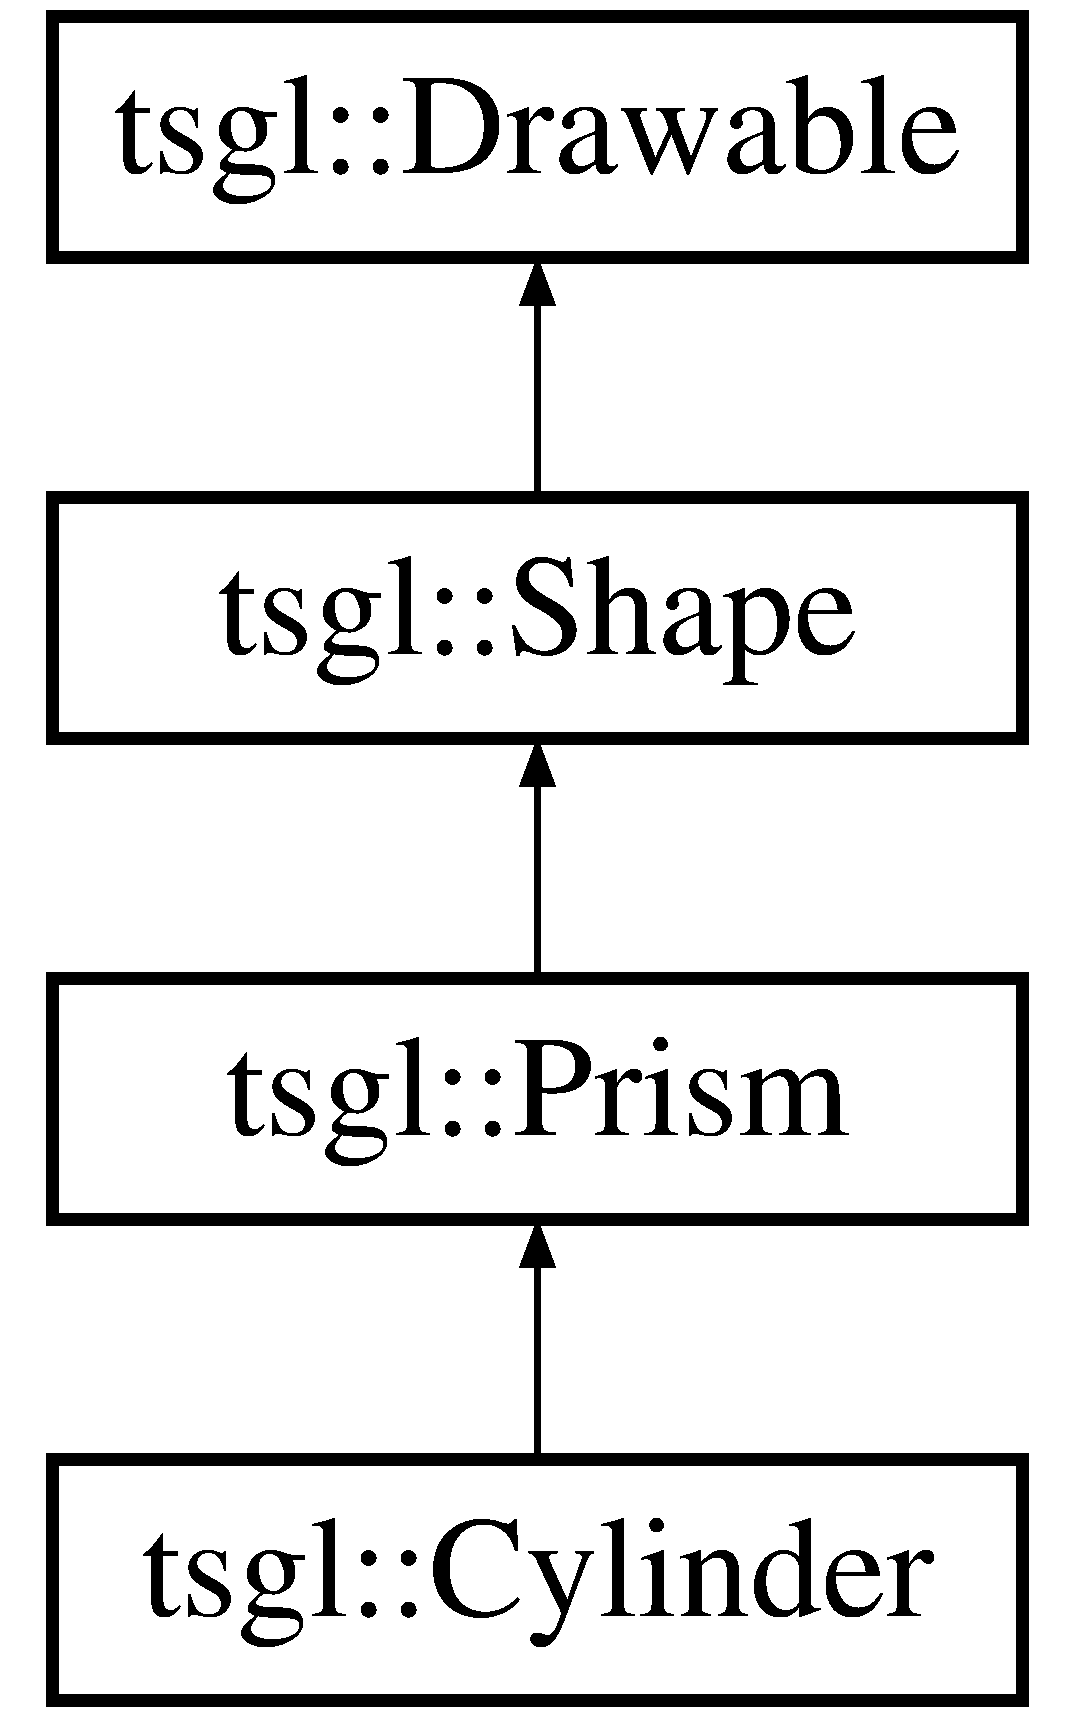
\includegraphics[height=4.000000cm]{classtsgl_1_1_cylinder}
\end{center}
\end{figure}
\subsection*{Public Member Functions}
\begin{DoxyCompactItemize}
\item 
\hyperlink{classtsgl_1_1_cylinder_a4b55b973ed7ac64dcda9a792a8b4d4f7}{Cylinder} (float x, float y, float z, G\+Lfloat height, G\+Lfloat radius, float yaw, float pitch, float roll, \hyperlink{structtsgl_1_1_color_float}{Color\+Float} c)
\begin{DoxyCompactList}\small\item\em Explicitly constructs a new \hyperlink{classtsgl_1_1_cylinder}{Cylinder}. \end{DoxyCompactList}\item 
\mbox{\Hypertarget{classtsgl_1_1_cylinder_aac310da5e5dd30ea7b41d028c185a050}\label{classtsgl_1_1_cylinder_aac310da5e5dd30ea7b41d028c185a050}} 
{\bfseries Cylinder} (float x, float y, float z, G\+Lfloat height, G\+Lfloat radius, float yaw, float pitch, float roll, \hyperlink{structtsgl_1_1_color_float}{Color\+Float} c\mbox{[}$\,$\mbox{]})
\item 
\mbox{\Hypertarget{classtsgl_1_1_cylinder_a0626417c3035e215b43fa2e38c966962}\label{classtsgl_1_1_cylinder_a0626417c3035e215b43fa2e38c966962}} 
virtual \hyperlink{classtsgl_1_1_cylinder_a0626417c3035e215b43fa2e38c966962}{$\sim$\+Cylinder} ()
\begin{DoxyCompactList}\small\item\em Destructor for the \hyperlink{classtsgl_1_1_cylinder}{Cylinder}. \end{DoxyCompactList}\end{DoxyCompactItemize}
\subsection*{Additional Inherited Members}


\subsection{Detailed Description}
Draw an arbitrary \hyperlink{classtsgl_1_1_cylinder}{Cylinder} with colored vertices. 

\hyperlink{classtsgl_1_1_cylinder}{Cylinder} is a class for holding vertex data for a \hyperlink{classtsgl_1_1_cylinder}{Cylinder}.

\hyperlink{classtsgl_1_1_cylinder}{Cylinder} is a subclass of \hyperlink{classtsgl_1_1_prism}{Prism} with a circular base. 

\subsection{Constructor \& Destructor Documentation}
\mbox{\Hypertarget{classtsgl_1_1_cylinder_a4b55b973ed7ac64dcda9a792a8b4d4f7}\label{classtsgl_1_1_cylinder_a4b55b973ed7ac64dcda9a792a8b4d4f7}} 
\index{tsgl\+::\+Cylinder@{tsgl\+::\+Cylinder}!Cylinder@{Cylinder}}
\index{Cylinder@{Cylinder}!tsgl\+::\+Cylinder@{tsgl\+::\+Cylinder}}
\subsubsection{\texorpdfstring{Cylinder()}{Cylinder()}}
{\footnotesize\ttfamily tsgl\+::\+Cylinder\+::\+Cylinder (\begin{DoxyParamCaption}\item[{float}]{x,  }\item[{float}]{y,  }\item[{float}]{z,  }\item[{G\+Lfloat}]{height,  }\item[{G\+Lfloat}]{radius,  }\item[{float}]{yaw,  }\item[{float}]{pitch,  }\item[{float}]{roll,  }\item[{\hyperlink{structtsgl_1_1_color_float}{Color\+Float}}]{c }\end{DoxyParamCaption})}



Explicitly constructs a new \hyperlink{classtsgl_1_1_cylinder}{Cylinder}. 

Explicit constructor for a \hyperlink{classtsgl_1_1_cylinder}{Cylinder} object. 
\begin{DoxyParams}{Parameters}
{\em x} & The x coordinate of the center of the \hyperlink{classtsgl_1_1_cylinder}{Cylinder}. \\
\hline
{\em y} & The y coordinate of the center of the \hyperlink{classtsgl_1_1_cylinder}{Cylinder}. \\
\hline
{\em z} & The z coordinate of the center of the \hyperlink{classtsgl_1_1_cylinder}{Cylinder}. \\
\hline
{\em height} & The height of the \hyperlink{classtsgl_1_1_cylinder}{Cylinder}. \\
\hline
{\em radius} & The radius of the \hyperlink{classtsgl_1_1_cylinder}{Cylinder}\textquotesingle{}s circular base. \\
\hline
{\em yaw} & The \hyperlink{classtsgl_1_1_cylinder}{Cylinder}\textquotesingle{}s yaw. \\
\hline
{\em pitch} & The \hyperlink{classtsgl_1_1_cylinder}{Cylinder}\textquotesingle{}s pitch. \\
\hline
{\em roll} & The \hyperlink{classtsgl_1_1_cylinder}{Cylinder}\textquotesingle{}s roll. \\
\hline
{\em c} & A \hyperlink{structtsgl_1_1_color_float}{Color\+Float} for the \hyperlink{classtsgl_1_1_cylinder}{Cylinder}\textquotesingle{}s vertex colors. \\
\hline
\end{DoxyParams}
\begin{DoxyWarning}{Warning}
An invariant is held where if length, width, or height isn\textquotesingle{}t positive then an error message is given. 
\end{DoxyWarning}
\begin{DoxyReturn}{Returns}
A new \hyperlink{classtsgl_1_1_cylinder}{Cylinder} with a buffer for storing the specified numbered of vertices. 
\end{DoxyReturn}


The documentation for this class was generated from the following files\+:\begin{DoxyCompactItemize}
\item 
Cylinder.\+h\item 
Cylinder.\+cpp\end{DoxyCompactItemize}

\hypertarget{classtsgl_1_1_drawable}{}\section{tsgl\+:\+:Drawable Class Reference}
\label{classtsgl_1_1_drawable}\index{tsgl\+::\+Drawable@{tsgl\+::\+Drawable}}


A class for drawing objects onto a \hyperlink{classtsgl_1_1_canvas}{Canvas} or \hyperlink{classtsgl_1_1_cartesian_canvas}{Cartesian\+Canvas}.  




{\ttfamily \#include $<$Drawable.\+h$>$}

Inheritance diagram for tsgl\+:\+:Drawable\+:\begin{figure}[H]
\begin{center}
\leavevmode
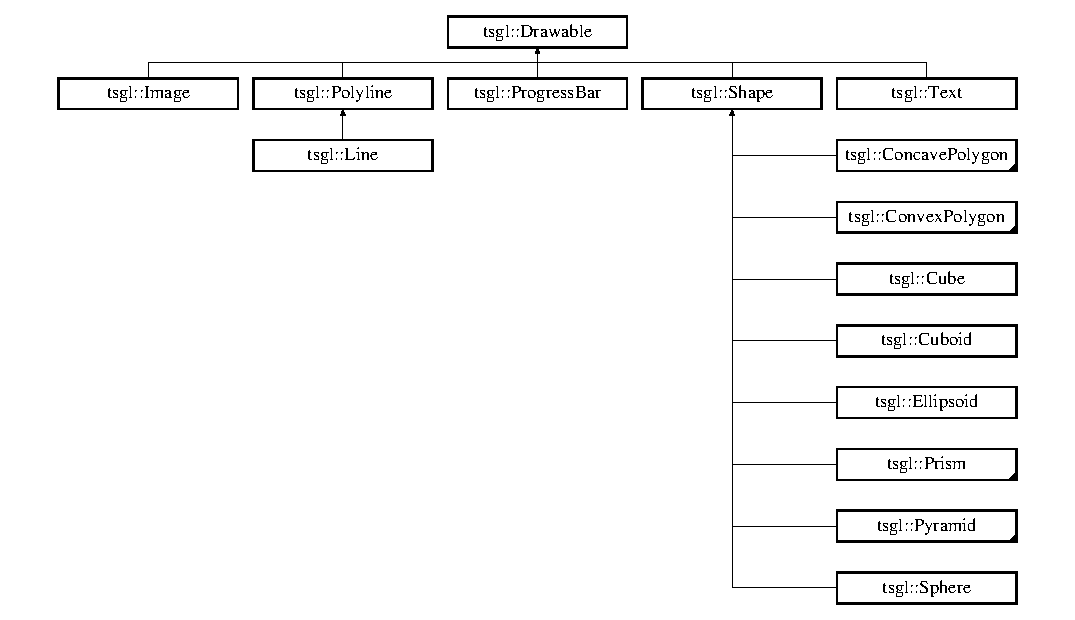
\includegraphics[height=7.887324cm]{classtsgl_1_1_drawable}
\end{center}
\end{figure}
\subsection*{Public Member Functions}
\begin{DoxyCompactItemize}
\item 
\hyperlink{classtsgl_1_1_drawable_a3a1394a83d01e3036b9eaf67dd5f56e6}{Drawable} (float x, float y, float z, float yaw, float pitch, float roll)
\begin{DoxyCompactList}\small\item\em Constructs a new \hyperlink{classtsgl_1_1_drawable}{Drawable}. \end{DoxyCompactList}\item 
\mbox{\Hypertarget{classtsgl_1_1_drawable_a0c1fc1a3588438c2884a489bbeba83c5}\label{classtsgl_1_1_drawable_a0c1fc1a3588438c2884a489bbeba83c5}} 
virtual void {\bfseries draw} (Shader $\ast$shader)=0
\item 
virtual void \hyperlink{classtsgl_1_1_drawable_a5f3c278c5f0fb64ac285ee8326c87987}{change\+X\+By} (float deltaX)
\begin{DoxyCompactList}\small\item\em Alters the \hyperlink{classtsgl_1_1_drawable}{Drawable}\textquotesingle{}s x position. \end{DoxyCompactList}\item 
virtual void \hyperlink{classtsgl_1_1_drawable_a4590b6d35aab302e59e9e7581ecd0997}{change\+Y\+By} (float deltaY)
\begin{DoxyCompactList}\small\item\em Alters the \hyperlink{classtsgl_1_1_drawable}{Drawable}\textquotesingle{}s y position. \end{DoxyCompactList}\item 
virtual void \hyperlink{classtsgl_1_1_drawable_a4497615a4e1e03c40a745fd80c1f51e0}{change\+Z\+By} (float deltaZ)
\begin{DoxyCompactList}\small\item\em Alters the \hyperlink{classtsgl_1_1_drawable}{Drawable}\textquotesingle{}s z position. \end{DoxyCompactList}\item 
virtual void \hyperlink{classtsgl_1_1_drawable_a5e93ed0fd3bd02ec1d77645666bfedb9}{change\+Center\+By} (float deltaX, float deltaY, float deltaZ)
\begin{DoxyCompactList}\small\item\em Alters the \hyperlink{classtsgl_1_1_drawable}{Drawable}\textquotesingle{}s vertex locations. \end{DoxyCompactList}\item 
virtual void \hyperlink{classtsgl_1_1_drawable_a100ed2db1357cd6bae7f991fcc353b8a}{set\+CenterX} (float x)
\begin{DoxyCompactList}\small\item\em Sets the \hyperlink{classtsgl_1_1_drawable}{Drawable}\textquotesingle{}s x position. \end{DoxyCompactList}\item 
virtual void \hyperlink{classtsgl_1_1_drawable_a389f768e42b01bf0553120c39e079a52}{set\+CenterY} (float y)
\begin{DoxyCompactList}\small\item\em Sets the \hyperlink{classtsgl_1_1_drawable}{Drawable}\textquotesingle{}s y position. \end{DoxyCompactList}\item 
virtual void \hyperlink{classtsgl_1_1_drawable_a4fe0cabf3863d81fd9889975a0580b9b}{set\+CenterZ} (float z)
\begin{DoxyCompactList}\small\item\em Sets the \hyperlink{classtsgl_1_1_drawable}{Drawable}\textquotesingle{}s z position. \end{DoxyCompactList}\item 
virtual void \hyperlink{classtsgl_1_1_drawable_aba0399448063c05ea6b01c63abf81a59}{set\+Center} (float x, float y, float z)
\begin{DoxyCompactList}\small\item\em Moves the \hyperlink{classtsgl_1_1_drawable}{Drawable} to new coordinates. \end{DoxyCompactList}\item 
virtual void \hyperlink{classtsgl_1_1_drawable_aaf7dbc52fdce998927f4459e6f235111}{set\+Yaw} (float yaw)
\begin{DoxyCompactList}\small\item\em Mutator for the \hyperlink{classtsgl_1_1_drawable}{Drawable}\textquotesingle{}s yaw. \end{DoxyCompactList}\item 
virtual void \hyperlink{classtsgl_1_1_drawable_a7857e9c90950854f76bf5967d0957367}{set\+Pitch} (float pitch)
\begin{DoxyCompactList}\small\item\em Mutator for the \hyperlink{classtsgl_1_1_drawable}{Drawable}\textquotesingle{}s pitch. \end{DoxyCompactList}\item 
virtual void \hyperlink{classtsgl_1_1_drawable_a7a99b21ab628ab11cdf5289ece1adf50}{set\+Roll} (float roll)
\begin{DoxyCompactList}\small\item\em Mutator for the \hyperlink{classtsgl_1_1_drawable}{Drawable}\textquotesingle{}s roll. \end{DoxyCompactList}\item 
virtual void \hyperlink{classtsgl_1_1_drawable_a127514372e6bd4b652fd384e27a944de}{set\+Yaw\+Pitch\+Roll} (float yaw, float pitch, float roll)
\begin{DoxyCompactList}\small\item\em Mutator for the yaw, pitch, and roll of the \hyperlink{classtsgl_1_1_drawable}{Drawable}. \end{DoxyCompactList}\item 
virtual void \hyperlink{classtsgl_1_1_drawable_a3a57e4a919a30931942d5f5f20f5647c}{change\+Yaw\+By} (float delta\+Yaw)
\begin{DoxyCompactList}\small\item\em Alters the \hyperlink{classtsgl_1_1_drawable}{Drawable}\textquotesingle{}s yaw by a specified amount. \end{DoxyCompactList}\item 
virtual void \hyperlink{classtsgl_1_1_drawable_a5cf7b8412046388eec3e518e99991646}{change\+Pitch\+By} (float delta\+Pitch)
\begin{DoxyCompactList}\small\item\em Alters the \hyperlink{classtsgl_1_1_drawable}{Drawable}\textquotesingle{}s pitch by a specified amount. \end{DoxyCompactList}\item 
virtual void \hyperlink{classtsgl_1_1_drawable_add43efbe60acaab91cf425facc68363a}{change\+Roll\+By} (float delta\+Roll)
\begin{DoxyCompactList}\small\item\em Alters the \hyperlink{classtsgl_1_1_drawable}{Drawable}\textquotesingle{}s roll by a specified amount. \end{DoxyCompactList}\item 
virtual void \hyperlink{classtsgl_1_1_drawable_af8541a8069354d047580676c51fa6942}{change\+Yaw\+Pitch\+Roll\+By} (float delta\+Yaw, float delta\+Pitch, float delta\+Roll)
\begin{DoxyCompactList}\small\item\em Alters the \hyperlink{classtsgl_1_1_drawable}{Drawable}\textquotesingle{}s yaw, pitch, and roll by a specified amount. \end{DoxyCompactList}\item 
virtual void \hyperlink{classtsgl_1_1_drawable_a7de462cb3293cba7beee25c8a0370891}{set\+Rotation\+PointX} (float x)
\begin{DoxyCompactList}\small\item\em Virtual mutator that changes the rotation point of the \hyperlink{classtsgl_1_1_drawable}{Drawable}\textquotesingle{}s x value. \end{DoxyCompactList}\item 
virtual void \hyperlink{classtsgl_1_1_drawable_a9576c059c277e1e936b5de228c0d59cf}{set\+Rotation\+PointY} (float y)
\begin{DoxyCompactList}\small\item\em Virtual mutator that changes the rotation point of the \hyperlink{classtsgl_1_1_drawable}{Drawable}\textquotesingle{}s y value. \end{DoxyCompactList}\item 
virtual void \hyperlink{classtsgl_1_1_drawable_a5293782ce59f1aff49defa38945ec6bb}{set\+Rotation\+PointZ} (float z)
\begin{DoxyCompactList}\small\item\em Virtual mutator that changes the rotation point of the \hyperlink{classtsgl_1_1_drawable}{Drawable}\textquotesingle{}s z value. \end{DoxyCompactList}\item 
virtual void \hyperlink{classtsgl_1_1_drawable_a9f99fff756caeac2e9f0cfa9cf30354f}{set\+Rotation\+Point} (float x, float y, float z)
\begin{DoxyCompactList}\small\item\em Sets the point around which \hyperlink{classtsgl_1_1_drawable}{Drawable} is rotated. \end{DoxyCompactList}\item 
virtual float \hyperlink{classtsgl_1_1_drawable_a170ce95eaae8b19532420e42e9eb8abf}{get\+CenterX} ()
\begin{DoxyCompactList}\small\item\em Accessor for the center x-\/coordinate of the \hyperlink{classtsgl_1_1_drawable}{Drawable}. \end{DoxyCompactList}\item 
virtual float \hyperlink{classtsgl_1_1_drawable_ad78d781f078bab0f458892757f100e7f}{get\+CenterY} ()
\begin{DoxyCompactList}\small\item\em Accessor for the center z-\/coordinate of the \hyperlink{classtsgl_1_1_drawable}{Drawable}. \end{DoxyCompactList}\item 
virtual float \hyperlink{classtsgl_1_1_drawable_a6a6c0441d94ffebd149f88ae3ab87ced}{get\+CenterZ} ()
\begin{DoxyCompactList}\small\item\em Accessor for the center z-\/coordinate of the \hyperlink{classtsgl_1_1_drawable}{Drawable}. \end{DoxyCompactList}\item 
virtual float \hyperlink{classtsgl_1_1_drawable_a9560ac32d0e19ee79b163c17f163cbb9}{get\+Yaw} ()
\begin{DoxyCompactList}\small\item\em Accessor for the Yaw of the \hyperlink{classtsgl_1_1_drawable}{Drawable}. \end{DoxyCompactList}\item 
virtual float \hyperlink{classtsgl_1_1_drawable_a124df4cd376a550dd52a2b8ed7dd3151}{get\+Pitch} ()
\begin{DoxyCompactList}\small\item\em Accessor for the Pitch of the \hyperlink{classtsgl_1_1_drawable}{Drawable}. \end{DoxyCompactList}\item 
virtual float \hyperlink{classtsgl_1_1_drawable_a311c8e3530138a5d377981cb759d06f3}{get\+Roll} ()
\begin{DoxyCompactList}\small\item\em Accessor for the Roll of the \hyperlink{classtsgl_1_1_drawable}{Drawable}. \end{DoxyCompactList}\item 
virtual float \hyperlink{classtsgl_1_1_drawable_a24835632306f5d78f4e4da96f48937da}{get\+Rotation\+PointX} ()
\begin{DoxyCompactList}\small\item\em Accessor for the rotation x-\/coordinate of the \hyperlink{classtsgl_1_1_drawable}{Drawable}. \end{DoxyCompactList}\item 
virtual float \hyperlink{classtsgl_1_1_drawable_a6a7876f0056f13aa3642c7beaf5949e3}{get\+Rotation\+PointY} ()
\begin{DoxyCompactList}\small\item\em Accessor for the rotation y-\/coordinate of the \hyperlink{classtsgl_1_1_drawable}{Drawable}. \end{DoxyCompactList}\item 
virtual float \hyperlink{classtsgl_1_1_drawable_a755bfd7fc04feb04f1932c0e0886c8e5}{get\+Rotation\+PointZ} ()
\begin{DoxyCompactList}\small\item\em Accessor for the rotation z-\/coordinate of the \hyperlink{classtsgl_1_1_drawable}{Drawable}. \end{DoxyCompactList}\item 
virtual bool \hyperlink{classtsgl_1_1_drawable_a98562ec95c8621ba9b46d7bd0c0ffece}{is\+Processed} ()
\begin{DoxyCompactList}\small\item\em Accessor that returns if \hyperlink{classtsgl_1_1_drawable}{Drawable} is processed and ready to be drawn. \end{DoxyCompactList}\item 
virtual unsigned int \hyperlink{classtsgl_1_1_drawable_a2985b1872024a4c0469e9953c60db728}{get\+Shader\+Type} ()
\begin{DoxyCompactList}\small\item\em Accessor that returns a value corresponding to a certain shader in \hyperlink{classtsgl_1_1_canvas}{Canvas}. \end{DoxyCompactList}\item 
virtual float \hyperlink{classtsgl_1_1_drawable_aa153a0c0a4eaaa9bf4b7640508d58850}{get\+Alpha} ()
\begin{DoxyCompactList}\small\item\em Accessor that returns \hyperlink{classtsgl_1_1_drawable}{Drawable}\textquotesingle{}s alpha value. \end{DoxyCompactList}\end{DoxyCompactItemize}
\subsection*{Protected Member Functions}
\begin{DoxyCompactItemize}
\item 
bool \hyperlink{classtsgl_1_1_drawable_a21c86457e72d4ce01309dff922e23ab5}{center\+Matches\+Rotation\+Point} ()
\begin{DoxyCompactList}\small\item\em Protected helper method that determines if the \hyperlink{classtsgl_1_1_drawable}{Drawable}\textquotesingle{}s center matches its rotation point. \end{DoxyCompactList}\end{DoxyCompactItemize}
\subsection*{Protected Attributes}
\begin{DoxyCompactItemize}
\item 
\mbox{\Hypertarget{classtsgl_1_1_drawable_a598f96849973e9cfdbf68d0e2826716b}\label{classtsgl_1_1_drawable_a598f96849973e9cfdbf68d0e2826716b}} 
std\+::mutex \hyperlink{classtsgl_1_1_drawable_a598f96849973e9cfdbf68d0e2826716b}{attrib\+Mutex}
\begin{DoxyCompactList}\small\item\em Protects the attributes of the \hyperlink{classtsgl_1_1_drawable}{Drawable} from being accessed while simultaneously being changed. \end{DoxyCompactList}\item 
\mbox{\Hypertarget{classtsgl_1_1_drawable_a9521a664f36ac95c7cf4237fed0b6c6c}\label{classtsgl_1_1_drawable_a9521a664f36ac95c7cf4237fed0b6c6c}} 
G\+Lfloat $\ast$ {\bfseries vertices}
\item 
\mbox{\Hypertarget{classtsgl_1_1_drawable_a753f3abfce4fc9b5aa598e9dea3412d1}\label{classtsgl_1_1_drawable_a753f3abfce4fc9b5aa598e9dea3412d1}} 
float {\bfseries my\+Current\+Yaw}
\item 
\mbox{\Hypertarget{classtsgl_1_1_drawable_a22179a40f7d0c5470f7f2d81f38bf31b}\label{classtsgl_1_1_drawable_a22179a40f7d0c5470f7f2d81f38bf31b}} 
float {\bfseries my\+Current\+Pitch}
\item 
\mbox{\Hypertarget{classtsgl_1_1_drawable_aed934d160d037c2f151b20a7a9b4896d}\label{classtsgl_1_1_drawable_aed934d160d037c2f151b20a7a9b4896d}} 
float {\bfseries my\+Current\+Roll}
\item 
\mbox{\Hypertarget{classtsgl_1_1_drawable_ae77c6e6f8d1a05e9e33e9d81010b7ab7}\label{classtsgl_1_1_drawable_ae77c6e6f8d1a05e9e33e9d81010b7ab7}} 
float {\bfseries my\+X\+Scale}
\item 
\mbox{\Hypertarget{classtsgl_1_1_drawable_a06f06101db328c6eaa4be3eb5c24b171}\label{classtsgl_1_1_drawable_a06f06101db328c6eaa4be3eb5c24b171}} 
float {\bfseries my\+Y\+Scale}
\item 
\mbox{\Hypertarget{classtsgl_1_1_drawable_aafb57cc94337b39bed9aed2f5985ae06}\label{classtsgl_1_1_drawable_aafb57cc94337b39bed9aed2f5985ae06}} 
float {\bfseries my\+Z\+Scale}
\item 
\mbox{\Hypertarget{classtsgl_1_1_drawable_a9b6135146dfb6d5afd51f14805088e85}\label{classtsgl_1_1_drawable_a9b6135146dfb6d5afd51f14805088e85}} 
float {\bfseries my\+Rotation\+PointX}
\item 
\mbox{\Hypertarget{classtsgl_1_1_drawable_afc85968c03eb68cdc3a1648986d4539f}\label{classtsgl_1_1_drawable_afc85968c03eb68cdc3a1648986d4539f}} 
float {\bfseries my\+Rotation\+PointY}
\item 
\mbox{\Hypertarget{classtsgl_1_1_drawable_ab18192d302c84c302ad4fa55248c1064}\label{classtsgl_1_1_drawable_ab18192d302c84c302ad4fa55248c1064}} 
float {\bfseries my\+Rotation\+PointZ}
\item 
\mbox{\Hypertarget{classtsgl_1_1_drawable_a2c45b9c3f4a2afba4270aa9f40eb82de}\label{classtsgl_1_1_drawable_a2c45b9c3f4a2afba4270aa9f40eb82de}} 
float {\bfseries my\+CenterX}
\item 
\mbox{\Hypertarget{classtsgl_1_1_drawable_a1d8726633a9303ca13530e8973662aff}\label{classtsgl_1_1_drawable_a1d8726633a9303ca13530e8973662aff}} 
float {\bfseries my\+CenterY}
\item 
\mbox{\Hypertarget{classtsgl_1_1_drawable_a59cf4ffb4550796ca2d2d1e29345b8de}\label{classtsgl_1_1_drawable_a59cf4ffb4550796ca2d2d1e29345b8de}} 
float {\bfseries my\+CenterZ}
\item 
\mbox{\Hypertarget{classtsgl_1_1_drawable_a3dd25b680812efbc48e4340cff5e6c67}\label{classtsgl_1_1_drawable_a3dd25b680812efbc48e4340cff5e6c67}} 
bool {\bfseries init} = false
\item 
\mbox{\Hypertarget{classtsgl_1_1_drawable_a4983a31b4e53ff6fff025b7dd61ffdc8}\label{classtsgl_1_1_drawable_a4983a31b4e53ff6fff025b7dd61ffdc8}} 
unsigned int {\bfseries shader\+Type} = S\+H\+A\+P\+E\+\_\+\+S\+H\+A\+D\+E\+R\+\_\+\+T\+Y\+PE
\item 
\mbox{\Hypertarget{classtsgl_1_1_drawable_af54a92431f81300879dddc70e2673270}\label{classtsgl_1_1_drawable_af54a92431f81300879dddc70e2673270}} 
G\+Lfloat {\bfseries my\+Alpha} = 0.\+0
\end{DoxyCompactItemize}


\subsection{Detailed Description}
A class for drawing objects onto a \hyperlink{classtsgl_1_1_canvas}{Canvas} or \hyperlink{classtsgl_1_1_cartesian_canvas}{Cartesian\+Canvas}. 

\begin{DoxyWarning}{Warning}
{\bfseries {\itshape Though extending this class must be allowed due to the way the code is set up, attempting to do so could potentially mess up the internal GL calls the library uses. Proceed with great caution.}}
\end{DoxyWarning}
\hyperlink{classtsgl_1_1_drawable}{Drawable} provides a base class for drawing 3D objects to a \hyperlink{classtsgl_1_1_canvas}{Canvas} or \hyperlink{classtsgl_1_1_cartesian_canvas}{Cartesian\+Canvas}. \begin{DoxyNote}{Note}
\hyperlink{classtsgl_1_1_drawable}{Drawable} is abstract, and must be extended by the user.
\end{DoxyNote}
{\ttfamily vertices} should be an array of floating point values in T\+S\+GL\textquotesingle{}s vertex format.

{\ttfamily numberofvertices} should be the actual integer number of vertices to be drawn (e.\+g., {\itshape 36} for a cube).

{\ttfamily geometry\+Type} should be one of GL\textquotesingle{}s primitive drawing modes. See \href{https://www.opengl.org/sdk/docs/man2/xhtml/glBegin.xml}{\tt https\+://www.\+opengl.\+org/sdk/docs/man2/xhtml/gl\+Begin.\+xml} for further information.

Theoretically, you could potentially extend the \hyperlink{classtsgl_1_1_drawable}{Drawable} class so that you can create another \hyperlink{classtsgl_1_1_drawable}{Drawable} class that suits your needs.

However, this is not recommended for normal use of the T\+S\+GL library. 

\subsection{Constructor \& Destructor Documentation}
\mbox{\Hypertarget{classtsgl_1_1_drawable_a3a1394a83d01e3036b9eaf67dd5f56e6}\label{classtsgl_1_1_drawable_a3a1394a83d01e3036b9eaf67dd5f56e6}} 
\index{tsgl\+::\+Drawable@{tsgl\+::\+Drawable}!Drawable@{Drawable}}
\index{Drawable@{Drawable}!tsgl\+::\+Drawable@{tsgl\+::\+Drawable}}
\subsubsection{\texorpdfstring{Drawable()}{Drawable()}}
{\footnotesize\ttfamily tsgl\+::\+Drawable\+::\+Drawable (\begin{DoxyParamCaption}\item[{float}]{x,  }\item[{float}]{y,  }\item[{float}]{z,  }\item[{float}]{yaw,  }\item[{float}]{pitch,  }\item[{float}]{roll }\end{DoxyParamCaption})}



Constructs a new \hyperlink{classtsgl_1_1_drawable}{Drawable}. 


\begin{DoxyItemize}
\item Usually {\ttfamily vertices} is filled with floating point values that represent the vertices of the \hyperlink{classtsgl_1_1_drawable}{Drawable} to be drawn.
\item You may define other items in the constructor that pertain to the attributes of the subclass that is extending \hyperlink{classtsgl_1_1_drawable}{Drawable}.
\item At a minimum, you {\itshape M\+U\+ST} fill an array of floating point values that pertain to the vertices of the \hyperlink{classtsgl_1_1_drawable}{Drawable}. \begin{DoxyWarning}{Warning}
{\bfseries You {\itshape must} inherit the parent\textquotesingle{}s constructor if you are extending \hyperlink{classtsgl_1_1_drawable}{Drawable}.} 
\end{DoxyWarning}
\begin{DoxyNote}{Note}
Refer to the \hyperlink{classtsgl_1_1_drawable}{Drawable} class description for more details. 
\end{DoxyNote}

\end{DoxyItemize}

Referenced by center\+Matches\+Rotation\+Point().



\subsection{Member Function Documentation}
\mbox{\Hypertarget{classtsgl_1_1_drawable_a21c86457e72d4ce01309dff922e23ab5}\label{classtsgl_1_1_drawable_a21c86457e72d4ce01309dff922e23ab5}} 
\index{tsgl\+::\+Drawable@{tsgl\+::\+Drawable}!center\+Matches\+Rotation\+Point@{center\+Matches\+Rotation\+Point}}
\index{center\+Matches\+Rotation\+Point@{center\+Matches\+Rotation\+Point}!tsgl\+::\+Drawable@{tsgl\+::\+Drawable}}
\subsubsection{\texorpdfstring{center\+Matches\+Rotation\+Point()}{centerMatchesRotationPoint()}}
{\footnotesize\ttfamily bool tsgl\+::\+Drawable\+::center\+Matches\+Rotation\+Point (\begin{DoxyParamCaption}{ }\end{DoxyParamCaption})\hspace{0.3cm}{\ttfamily [inline]}, {\ttfamily [protected]}}



Protected helper method that determines if the \hyperlink{classtsgl_1_1_drawable}{Drawable}\textquotesingle{}s center matches its rotation point. 

Checks to see if my\+CenterX == my\+Rotation\+PointX, my\+CenterY == my\+Rotation\+PointY, my\+CenterZ == my\+Rotation\+PointZ \begin{DoxyReturn}{Returns}
True if all three coordinates match their respective others, false otherwise. 
\end{DoxyReturn}


Referenced by change\+Center\+By(), change\+X\+By(), change\+Y\+By(), change\+Z\+By(), get\+Center\+X(), get\+Center\+Y(), get\+Center\+Z(), set\+Center(), set\+Center\+X(), set\+Center\+Y(), set\+Center\+Z(), tsgl\+::\+Line\+::set\+First\+Endpoint(), tsgl\+::\+Arrow\+::set\+First\+Endpoint(), tsgl\+::\+Line\+::set\+Second\+Endpoint(), and tsgl\+::\+Arrow\+::set\+Second\+Endpoint().

\mbox{\Hypertarget{classtsgl_1_1_drawable_a5e93ed0fd3bd02ec1d77645666bfedb9}\label{classtsgl_1_1_drawable_a5e93ed0fd3bd02ec1d77645666bfedb9}} 
\index{tsgl\+::\+Drawable@{tsgl\+::\+Drawable}!change\+Center\+By@{change\+Center\+By}}
\index{change\+Center\+By@{change\+Center\+By}!tsgl\+::\+Drawable@{tsgl\+::\+Drawable}}
\subsubsection{\texorpdfstring{change\+Center\+By()}{changeCenterBy()}}
{\footnotesize\ttfamily void tsgl\+::\+Drawable\+::change\+Center\+By (\begin{DoxyParamCaption}\item[{float}]{deltaX,  }\item[{float}]{deltaY,  }\item[{float}]{deltaZ }\end{DoxyParamCaption})\hspace{0.3cm}{\ttfamily [virtual]}}



Alters the \hyperlink{classtsgl_1_1_drawable}{Drawable}\textquotesingle{}s vertex locations. 


\begin{DoxyParams}{Parameters}
{\em deltaX} & The difference between the new and old vertex x coordinates. \\
\hline
{\em deltaY} & The difference between the new and old vertex y coordinates. \\
\hline
{\em deltaZ} & The difference between the new and old vertex z coordinates. \\
\hline
\end{DoxyParams}
\begin{DoxyWarning}{Warning}
This will also alter the \hyperlink{classtsgl_1_1_drawable}{Drawable}\textquotesingle{}s rotation point similarly if and only if the old rotation point was at the \hyperlink{classtsgl_1_1_drawable}{Drawable}\textquotesingle{}s old center. 
\end{DoxyWarning}


Referenced by center\+Matches\+Rotation\+Point().

\mbox{\Hypertarget{classtsgl_1_1_drawable_a5cf7b8412046388eec3e518e99991646}\label{classtsgl_1_1_drawable_a5cf7b8412046388eec3e518e99991646}} 
\index{tsgl\+::\+Drawable@{tsgl\+::\+Drawable}!change\+Pitch\+By@{change\+Pitch\+By}}
\index{change\+Pitch\+By@{change\+Pitch\+By}!tsgl\+::\+Drawable@{tsgl\+::\+Drawable}}
\subsubsection{\texorpdfstring{change\+Pitch\+By()}{changePitchBy()}}
{\footnotesize\ttfamily void tsgl\+::\+Drawable\+::change\+Pitch\+By (\begin{DoxyParamCaption}\item[{float}]{delta\+Pitch }\end{DoxyParamCaption})\hspace{0.3cm}{\ttfamily [virtual]}}



Alters the \hyperlink{classtsgl_1_1_drawable}{Drawable}\textquotesingle{}s pitch by a specified amount. 


\begin{DoxyParams}{Parameters}
{\em delta\+Pitch} & The change in pitch value for \hyperlink{classtsgl_1_1_drawable}{Drawable}. \\
\hline
\end{DoxyParams}


Referenced by center\+Matches\+Rotation\+Point().

\mbox{\Hypertarget{classtsgl_1_1_drawable_add43efbe60acaab91cf425facc68363a}\label{classtsgl_1_1_drawable_add43efbe60acaab91cf425facc68363a}} 
\index{tsgl\+::\+Drawable@{tsgl\+::\+Drawable}!change\+Roll\+By@{change\+Roll\+By}}
\index{change\+Roll\+By@{change\+Roll\+By}!tsgl\+::\+Drawable@{tsgl\+::\+Drawable}}
\subsubsection{\texorpdfstring{change\+Roll\+By()}{changeRollBy()}}
{\footnotesize\ttfamily void tsgl\+::\+Drawable\+::change\+Roll\+By (\begin{DoxyParamCaption}\item[{float}]{delta\+Roll }\end{DoxyParamCaption})\hspace{0.3cm}{\ttfamily [virtual]}}



Alters the \hyperlink{classtsgl_1_1_drawable}{Drawable}\textquotesingle{}s roll by a specified amount. 


\begin{DoxyParams}{Parameters}
{\em delta\+Roll} & The change in roll value for \hyperlink{classtsgl_1_1_drawable}{Drawable}. \\
\hline
\end{DoxyParams}


Referenced by center\+Matches\+Rotation\+Point().

\mbox{\Hypertarget{classtsgl_1_1_drawable_a5f3c278c5f0fb64ac285ee8326c87987}\label{classtsgl_1_1_drawable_a5f3c278c5f0fb64ac285ee8326c87987}} 
\index{tsgl\+::\+Drawable@{tsgl\+::\+Drawable}!change\+X\+By@{change\+X\+By}}
\index{change\+X\+By@{change\+X\+By}!tsgl\+::\+Drawable@{tsgl\+::\+Drawable}}
\subsubsection{\texorpdfstring{change\+X\+By()}{changeXBy()}}
{\footnotesize\ttfamily void tsgl\+::\+Drawable\+::change\+X\+By (\begin{DoxyParamCaption}\item[{float}]{deltaX }\end{DoxyParamCaption})\hspace{0.3cm}{\ttfamily [virtual]}}



Alters the \hyperlink{classtsgl_1_1_drawable}{Drawable}\textquotesingle{}s x position. 


\begin{DoxyParams}{Parameters}
{\em deltaX} & The difference between the new and old vertex x coordinates. \\
\hline
\end{DoxyParams}
\begin{DoxyWarning}{Warning}
This will also alter the \hyperlink{classtsgl_1_1_drawable}{Drawable}\textquotesingle{}s rotation point similarly if and only if the old rotation point was at the \hyperlink{classtsgl_1_1_drawable}{Drawable}\textquotesingle{}s old center. 
\end{DoxyWarning}


Referenced by center\+Matches\+Rotation\+Point().

\mbox{\Hypertarget{classtsgl_1_1_drawable_a3a57e4a919a30931942d5f5f20f5647c}\label{classtsgl_1_1_drawable_a3a57e4a919a30931942d5f5f20f5647c}} 
\index{tsgl\+::\+Drawable@{tsgl\+::\+Drawable}!change\+Yaw\+By@{change\+Yaw\+By}}
\index{change\+Yaw\+By@{change\+Yaw\+By}!tsgl\+::\+Drawable@{tsgl\+::\+Drawable}}
\subsubsection{\texorpdfstring{change\+Yaw\+By()}{changeYawBy()}}
{\footnotesize\ttfamily void tsgl\+::\+Drawable\+::change\+Yaw\+By (\begin{DoxyParamCaption}\item[{float}]{delta\+Yaw }\end{DoxyParamCaption})\hspace{0.3cm}{\ttfamily [virtual]}}



Alters the \hyperlink{classtsgl_1_1_drawable}{Drawable}\textquotesingle{}s yaw by a specified amount. 


\begin{DoxyParams}{Parameters}
{\em delta\+Yaw} & The change in yaw value for \hyperlink{classtsgl_1_1_drawable}{Drawable}. \\
\hline
\end{DoxyParams}


Referenced by center\+Matches\+Rotation\+Point().

\mbox{\Hypertarget{classtsgl_1_1_drawable_af8541a8069354d047580676c51fa6942}\label{classtsgl_1_1_drawable_af8541a8069354d047580676c51fa6942}} 
\index{tsgl\+::\+Drawable@{tsgl\+::\+Drawable}!change\+Yaw\+Pitch\+Roll\+By@{change\+Yaw\+Pitch\+Roll\+By}}
\index{change\+Yaw\+Pitch\+Roll\+By@{change\+Yaw\+Pitch\+Roll\+By}!tsgl\+::\+Drawable@{tsgl\+::\+Drawable}}
\subsubsection{\texorpdfstring{change\+Yaw\+Pitch\+Roll\+By()}{changeYawPitchRollBy()}}
{\footnotesize\ttfamily void tsgl\+::\+Drawable\+::change\+Yaw\+Pitch\+Roll\+By (\begin{DoxyParamCaption}\item[{float}]{delta\+Yaw,  }\item[{float}]{delta\+Pitch,  }\item[{float}]{delta\+Roll }\end{DoxyParamCaption})\hspace{0.3cm}{\ttfamily [virtual]}}



Alters the \hyperlink{classtsgl_1_1_drawable}{Drawable}\textquotesingle{}s yaw, pitch, and roll by a specified amount. 


\begin{DoxyParams}{Parameters}
{\em delta\+Yaw} & The change in yaw value for \hyperlink{classtsgl_1_1_drawable}{Drawable}. \\
\hline
{\em delta\+Pitch} & The change in pitch value for \hyperlink{classtsgl_1_1_drawable}{Drawable}. \\
\hline
{\em delta\+Roll} & The change in roll value for \hyperlink{classtsgl_1_1_drawable}{Drawable}. \\
\hline
\end{DoxyParams}


Referenced by center\+Matches\+Rotation\+Point().

\mbox{\Hypertarget{classtsgl_1_1_drawable_a4590b6d35aab302e59e9e7581ecd0997}\label{classtsgl_1_1_drawable_a4590b6d35aab302e59e9e7581ecd0997}} 
\index{tsgl\+::\+Drawable@{tsgl\+::\+Drawable}!change\+Y\+By@{change\+Y\+By}}
\index{change\+Y\+By@{change\+Y\+By}!tsgl\+::\+Drawable@{tsgl\+::\+Drawable}}
\subsubsection{\texorpdfstring{change\+Y\+By()}{changeYBy()}}
{\footnotesize\ttfamily void tsgl\+::\+Drawable\+::change\+Y\+By (\begin{DoxyParamCaption}\item[{float}]{deltaY }\end{DoxyParamCaption})\hspace{0.3cm}{\ttfamily [virtual]}}



Alters the \hyperlink{classtsgl_1_1_drawable}{Drawable}\textquotesingle{}s y position. 


\begin{DoxyParams}{Parameters}
{\em deltaY} & The difference between the new and old vertex y coordinates. \\
\hline
\end{DoxyParams}
\begin{DoxyWarning}{Warning}
This will also alter the \hyperlink{classtsgl_1_1_drawable}{Drawable}\textquotesingle{}s rotation point similarly if and only if the old rotation point was at the \hyperlink{classtsgl_1_1_drawable}{Drawable}\textquotesingle{}s old center. 
\end{DoxyWarning}


Referenced by center\+Matches\+Rotation\+Point(), and Paddle\+::move().

\mbox{\Hypertarget{classtsgl_1_1_drawable_a4497615a4e1e03c40a745fd80c1f51e0}\label{classtsgl_1_1_drawable_a4497615a4e1e03c40a745fd80c1f51e0}} 
\index{tsgl\+::\+Drawable@{tsgl\+::\+Drawable}!change\+Z\+By@{change\+Z\+By}}
\index{change\+Z\+By@{change\+Z\+By}!tsgl\+::\+Drawable@{tsgl\+::\+Drawable}}
\subsubsection{\texorpdfstring{change\+Z\+By()}{changeZBy()}}
{\footnotesize\ttfamily void tsgl\+::\+Drawable\+::change\+Z\+By (\begin{DoxyParamCaption}\item[{float}]{deltaZ }\end{DoxyParamCaption})\hspace{0.3cm}{\ttfamily [virtual]}}



Alters the \hyperlink{classtsgl_1_1_drawable}{Drawable}\textquotesingle{}s z position. 


\begin{DoxyParams}{Parameters}
{\em deltaZ} & The difference between the new and old vertex z coordinates. \\
\hline
\end{DoxyParams}
\begin{DoxyWarning}{Warning}
This will also alter the \hyperlink{classtsgl_1_1_drawable}{Drawable}\textquotesingle{}s rotation point similarly if and only if the old rotation point was at the \hyperlink{classtsgl_1_1_drawable}{Drawable}\textquotesingle{}s old center. 
\end{DoxyWarning}


Referenced by center\+Matches\+Rotation\+Point().

\mbox{\Hypertarget{classtsgl_1_1_drawable_aa153a0c0a4eaaa9bf4b7640508d58850}\label{classtsgl_1_1_drawable_aa153a0c0a4eaaa9bf4b7640508d58850}} 
\index{tsgl\+::\+Drawable@{tsgl\+::\+Drawable}!get\+Alpha@{get\+Alpha}}
\index{get\+Alpha@{get\+Alpha}!tsgl\+::\+Drawable@{tsgl\+::\+Drawable}}
\subsubsection{\texorpdfstring{get\+Alpha()}{getAlpha()}}
{\footnotesize\ttfamily virtual float tsgl\+::\+Drawable\+::get\+Alpha (\begin{DoxyParamCaption}{ }\end{DoxyParamCaption})\hspace{0.3cm}{\ttfamily [inline]}, {\ttfamily [virtual]}}



Accessor that returns \hyperlink{classtsgl_1_1_drawable}{Drawable}\textquotesingle{}s alpha value. 

Principally designed to be used within \hyperlink{classtsgl_1_1_canvas}{Canvas} for transparency sorting. 

Referenced by tsgl\+::\+Canvas\+::clear\+Object\+Buffer().

\mbox{\Hypertarget{classtsgl_1_1_drawable_a170ce95eaae8b19532420e42e9eb8abf}\label{classtsgl_1_1_drawable_a170ce95eaae8b19532420e42e9eb8abf}} 
\index{tsgl\+::\+Drawable@{tsgl\+::\+Drawable}!get\+CenterX@{get\+CenterX}}
\index{get\+CenterX@{get\+CenterX}!tsgl\+::\+Drawable@{tsgl\+::\+Drawable}}
\subsubsection{\texorpdfstring{get\+Center\+X()}{getCenterX()}}
{\footnotesize\ttfamily float tsgl\+::\+Drawable\+::get\+CenterX (\begin{DoxyParamCaption}{ }\end{DoxyParamCaption})\hspace{0.3cm}{\ttfamily [virtual]}}



Accessor for the center x-\/coordinate of the \hyperlink{classtsgl_1_1_drawable}{Drawable}. 

Returns the value of the my\+CenterX private variable, rotated by my\+Current\+Yaw, my\+Current\+Pitch, and my\+Current\+Roll about my\+Rotation\+PointX; \begin{DoxyNote}{Note}
See \href{https://math.stackexchange.com/questions/2093314/rotation-matrix-of-rotation-around-a-point-other-than-the-origin}{\tt https\+://math.\+stackexchange.\+com/questions/2093314/rotation-\/matrix-\/of-\/rotation-\/around-\/a-\/point-\/other-\/than-\/the-\/origin} 

and \href{http://planning.cs.uiuc.edu/node102.html}{\tt http\+://planning.\+cs.\+uiuc.\+edu/node102.\+html} for more more understanding. 
\end{DoxyNote}


Referenced by Consumer\+::act(), center\+Matches\+Rotation\+Point(), tsgl\+::\+Canvas\+::clear\+Object\+Buffer(), Philosopher3\+D\+::draw(), P\+C\+Thread\+::\+P\+C\+Thread(), Reader\+::\+Reader(), and Writer\+::\+Writer().

\mbox{\Hypertarget{classtsgl_1_1_drawable_ad78d781f078bab0f458892757f100e7f}\label{classtsgl_1_1_drawable_ad78d781f078bab0f458892757f100e7f}} 
\index{tsgl\+::\+Drawable@{tsgl\+::\+Drawable}!get\+CenterY@{get\+CenterY}}
\index{get\+CenterY@{get\+CenterY}!tsgl\+::\+Drawable@{tsgl\+::\+Drawable}}
\subsubsection{\texorpdfstring{get\+Center\+Y()}{getCenterY()}}
{\footnotesize\ttfamily float tsgl\+::\+Drawable\+::get\+CenterY (\begin{DoxyParamCaption}{ }\end{DoxyParamCaption})\hspace{0.3cm}{\ttfamily [virtual]}}



Accessor for the center z-\/coordinate of the \hyperlink{classtsgl_1_1_drawable}{Drawable}. 

Returns the value of the my\+CenterY private variable, rotated by my\+Current\+Yaw, my\+Current\+Pitch, and my\+Current\+Roll about my\+Rotation\+PointY; \begin{DoxyNote}{Note}
See \href{https://math.stackexchange.com/questions/2093314/rotation-matrix-of-rotation-around-a-point-other-than-the-origin}{\tt https\+://math.\+stackexchange.\+com/questions/2093314/rotation-\/matrix-\/of-\/rotation-\/around-\/a-\/point-\/other-\/than-\/the-\/origin} 

and \href{http://planning.cs.uiuc.edu/node102.html}{\tt http\+://planning.\+cs.\+uiuc.\+edu/node102.\+html} for more more understanding. 
\end{DoxyNote}


Referenced by Consumer\+::act(), center\+Matches\+Rotation\+Point(), tsgl\+::\+Canvas\+::clear\+Object\+Buffer(), Philosopher3\+D\+::draw(), P\+C\+Thread\+::\+P\+C\+Thread(), Reader\+::\+Reader(), and Writer\+::\+Writer().

\mbox{\Hypertarget{classtsgl_1_1_drawable_a6a6c0441d94ffebd149f88ae3ab87ced}\label{classtsgl_1_1_drawable_a6a6c0441d94ffebd149f88ae3ab87ced}} 
\index{tsgl\+::\+Drawable@{tsgl\+::\+Drawable}!get\+CenterZ@{get\+CenterZ}}
\index{get\+CenterZ@{get\+CenterZ}!tsgl\+::\+Drawable@{tsgl\+::\+Drawable}}
\subsubsection{\texorpdfstring{get\+Center\+Z()}{getCenterZ()}}
{\footnotesize\ttfamily float tsgl\+::\+Drawable\+::get\+CenterZ (\begin{DoxyParamCaption}{ }\end{DoxyParamCaption})\hspace{0.3cm}{\ttfamily [virtual]}}



Accessor for the center z-\/coordinate of the \hyperlink{classtsgl_1_1_drawable}{Drawable}. 

Returns the value of the my\+CenterZ private variable, rotated by my\+Current\+Yaw, my\+Current\+Pitch, and my\+Current\+Roll about my\+Rotation\+PointZ; \begin{DoxyNote}{Note}
See \href{https://math.stackexchange.com/questions/2093314/rotation-matrix-of-rotation-around-a-point-other-than-the-origin}{\tt https\+://math.\+stackexchange.\+com/questions/2093314/rotation-\/matrix-\/of-\/rotation-\/around-\/a-\/point-\/other-\/than-\/the-\/origin} 

and \href{http://planning.cs.uiuc.edu/node102.html}{\tt http\+://planning.\+cs.\+uiuc.\+edu/node102.\+html} for more more understanding. 
\end{DoxyNote}


Referenced by center\+Matches\+Rotation\+Point(), tsgl\+::\+Canvas\+::clear\+Object\+Buffer(), and Philosopher3\+D\+::draw().

\mbox{\Hypertarget{classtsgl_1_1_drawable_a124df4cd376a550dd52a2b8ed7dd3151}\label{classtsgl_1_1_drawable_a124df4cd376a550dd52a2b8ed7dd3151}} 
\index{tsgl\+::\+Drawable@{tsgl\+::\+Drawable}!get\+Pitch@{get\+Pitch}}
\index{get\+Pitch@{get\+Pitch}!tsgl\+::\+Drawable@{tsgl\+::\+Drawable}}
\subsubsection{\texorpdfstring{get\+Pitch()}{getPitch()}}
{\footnotesize\ttfamily virtual float tsgl\+::\+Drawable\+::get\+Pitch (\begin{DoxyParamCaption}{ }\end{DoxyParamCaption})\hspace{0.3cm}{\ttfamily [inline]}, {\ttfamily [virtual]}}



Accessor for the Pitch of the \hyperlink{classtsgl_1_1_drawable}{Drawable}. 

Returns the value of the my\+Current\+Pitch private variable. \mbox{\Hypertarget{classtsgl_1_1_drawable_a311c8e3530138a5d377981cb759d06f3}\label{classtsgl_1_1_drawable_a311c8e3530138a5d377981cb759d06f3}} 
\index{tsgl\+::\+Drawable@{tsgl\+::\+Drawable}!get\+Roll@{get\+Roll}}
\index{get\+Roll@{get\+Roll}!tsgl\+::\+Drawable@{tsgl\+::\+Drawable}}
\subsubsection{\texorpdfstring{get\+Roll()}{getRoll()}}
{\footnotesize\ttfamily virtual float tsgl\+::\+Drawable\+::get\+Roll (\begin{DoxyParamCaption}{ }\end{DoxyParamCaption})\hspace{0.3cm}{\ttfamily [inline]}, {\ttfamily [virtual]}}



Accessor for the Roll of the \hyperlink{classtsgl_1_1_drawable}{Drawable}. 

Returns the value of the my\+Current\+Roll private variable. \mbox{\Hypertarget{classtsgl_1_1_drawable_a24835632306f5d78f4e4da96f48937da}\label{classtsgl_1_1_drawable_a24835632306f5d78f4e4da96f48937da}} 
\index{tsgl\+::\+Drawable@{tsgl\+::\+Drawable}!get\+Rotation\+PointX@{get\+Rotation\+PointX}}
\index{get\+Rotation\+PointX@{get\+Rotation\+PointX}!tsgl\+::\+Drawable@{tsgl\+::\+Drawable}}
\subsubsection{\texorpdfstring{get\+Rotation\+Point\+X()}{getRotationPointX()}}
{\footnotesize\ttfamily virtual float tsgl\+::\+Drawable\+::get\+Rotation\+PointX (\begin{DoxyParamCaption}{ }\end{DoxyParamCaption})\hspace{0.3cm}{\ttfamily [inline]}, {\ttfamily [virtual]}}



Accessor for the rotation x-\/coordinate of the \hyperlink{classtsgl_1_1_drawable}{Drawable}. 

Returns the value of the my\+Rotation\+PointX private variable. \mbox{\Hypertarget{classtsgl_1_1_drawable_a6a7876f0056f13aa3642c7beaf5949e3}\label{classtsgl_1_1_drawable_a6a7876f0056f13aa3642c7beaf5949e3}} 
\index{tsgl\+::\+Drawable@{tsgl\+::\+Drawable}!get\+Rotation\+PointY@{get\+Rotation\+PointY}}
\index{get\+Rotation\+PointY@{get\+Rotation\+PointY}!tsgl\+::\+Drawable@{tsgl\+::\+Drawable}}
\subsubsection{\texorpdfstring{get\+Rotation\+Point\+Y()}{getRotationPointY()}}
{\footnotesize\ttfamily virtual float tsgl\+::\+Drawable\+::get\+Rotation\+PointY (\begin{DoxyParamCaption}{ }\end{DoxyParamCaption})\hspace{0.3cm}{\ttfamily [inline]}, {\ttfamily [virtual]}}



Accessor for the rotation y-\/coordinate of the \hyperlink{classtsgl_1_1_drawable}{Drawable}. 

Returns the value of the my\+Rotation\+PointY private variable. \mbox{\Hypertarget{classtsgl_1_1_drawable_a755bfd7fc04feb04f1932c0e0886c8e5}\label{classtsgl_1_1_drawable_a755bfd7fc04feb04f1932c0e0886c8e5}} 
\index{tsgl\+::\+Drawable@{tsgl\+::\+Drawable}!get\+Rotation\+PointZ@{get\+Rotation\+PointZ}}
\index{get\+Rotation\+PointZ@{get\+Rotation\+PointZ}!tsgl\+::\+Drawable@{tsgl\+::\+Drawable}}
\subsubsection{\texorpdfstring{get\+Rotation\+Point\+Z()}{getRotationPointZ()}}
{\footnotesize\ttfamily virtual float tsgl\+::\+Drawable\+::get\+Rotation\+PointZ (\begin{DoxyParamCaption}{ }\end{DoxyParamCaption})\hspace{0.3cm}{\ttfamily [inline]}, {\ttfamily [virtual]}}



Accessor for the rotation z-\/coordinate of the \hyperlink{classtsgl_1_1_drawable}{Drawable}. 

Returns the value of the my\+Rotation\+PointZ private variable. \mbox{\Hypertarget{classtsgl_1_1_drawable_a2985b1872024a4c0469e9953c60db728}\label{classtsgl_1_1_drawable_a2985b1872024a4c0469e9953c60db728}} 
\index{tsgl\+::\+Drawable@{tsgl\+::\+Drawable}!get\+Shader\+Type@{get\+Shader\+Type}}
\index{get\+Shader\+Type@{get\+Shader\+Type}!tsgl\+::\+Drawable@{tsgl\+::\+Drawable}}
\subsubsection{\texorpdfstring{get\+Shader\+Type()}{getShaderType()}}
{\footnotesize\ttfamily virtual unsigned int tsgl\+::\+Drawable\+::get\+Shader\+Type (\begin{DoxyParamCaption}{ }\end{DoxyParamCaption})\hspace{0.3cm}{\ttfamily [inline]}, {\ttfamily [virtual]}}



Accessor that returns a value corresponding to a certain shader in \hyperlink{classtsgl_1_1_canvas}{Canvas}. 

This function returns the value of the shader\+Type instance variable. 

Referenced by tsgl\+::\+Canvas\+::clear\+Object\+Buffer(), tsgl\+::\+Cartesian\+Background\+::draw(), and tsgl\+::\+Background\+::draw().

\mbox{\Hypertarget{classtsgl_1_1_drawable_a9560ac32d0e19ee79b163c17f163cbb9}\label{classtsgl_1_1_drawable_a9560ac32d0e19ee79b163c17f163cbb9}} 
\index{tsgl\+::\+Drawable@{tsgl\+::\+Drawable}!get\+Yaw@{get\+Yaw}}
\index{get\+Yaw@{get\+Yaw}!tsgl\+::\+Drawable@{tsgl\+::\+Drawable}}
\subsubsection{\texorpdfstring{get\+Yaw()}{getYaw()}}
{\footnotesize\ttfamily virtual float tsgl\+::\+Drawable\+::get\+Yaw (\begin{DoxyParamCaption}{ }\end{DoxyParamCaption})\hspace{0.3cm}{\ttfamily [inline]}, {\ttfamily [virtual]}}



Accessor for the Yaw of the \hyperlink{classtsgl_1_1_drawable}{Drawable}. 

Returns the value of the my\+Current\+Yaw private variable. \mbox{\Hypertarget{classtsgl_1_1_drawable_a98562ec95c8621ba9b46d7bd0c0ffece}\label{classtsgl_1_1_drawable_a98562ec95c8621ba9b46d7bd0c0ffece}} 
\index{tsgl\+::\+Drawable@{tsgl\+::\+Drawable}!is\+Processed@{is\+Processed}}
\index{is\+Processed@{is\+Processed}!tsgl\+::\+Drawable@{tsgl\+::\+Drawable}}
\subsubsection{\texorpdfstring{is\+Processed()}{isProcessed()}}
{\footnotesize\ttfamily virtual bool tsgl\+::\+Drawable\+::is\+Processed (\begin{DoxyParamCaption}{ }\end{DoxyParamCaption})\hspace{0.3cm}{\ttfamily [inline]}, {\ttfamily [virtual]}}



Accessor that returns if \hyperlink{classtsgl_1_1_drawable}{Drawable} is processed and ready to be drawn. 

This function returns true only if all vertices have been inserted into an array. 

Reimplemented in \hyperlink{classtsgl_1_1_shape_adf7724c786882b2bd4375c1e4807ed5d}{tsgl\+::\+Shape}, and \hyperlink{classtsgl_1_1_polyline_a9ce8dd308664600c31ef0047908c31d5}{tsgl\+::\+Polyline}.



Referenced by tsgl\+::\+Canvas\+::clear\+Object\+Buffer(), tsgl\+::\+Cartesian\+Background\+::draw(), and tsgl\+::\+Background\+::draw().

\mbox{\Hypertarget{classtsgl_1_1_drawable_aba0399448063c05ea6b01c63abf81a59}\label{classtsgl_1_1_drawable_aba0399448063c05ea6b01c63abf81a59}} 
\index{tsgl\+::\+Drawable@{tsgl\+::\+Drawable}!set\+Center@{set\+Center}}
\index{set\+Center@{set\+Center}!tsgl\+::\+Drawable@{tsgl\+::\+Drawable}}
\subsubsection{\texorpdfstring{set\+Center()}{setCenter()}}
{\footnotesize\ttfamily void tsgl\+::\+Drawable\+::set\+Center (\begin{DoxyParamCaption}\item[{float}]{x,  }\item[{float}]{y,  }\item[{float}]{z }\end{DoxyParamCaption})\hspace{0.3cm}{\ttfamily [virtual]}}



Moves the \hyperlink{classtsgl_1_1_drawable}{Drawable} to new coordinates. 


\begin{DoxyParams}{Parameters}
{\em x} & The new center x coordinate. \\
\hline
{\em y} & The new center y coordinate. \\
\hline
{\em z} & The new center z coordinate. \\
\hline
\end{DoxyParams}
\begin{DoxyWarning}{Warning}
This will also alter the \hyperlink{classtsgl_1_1_drawable}{Drawable}\textquotesingle{}s rotation point similarly if and only if the old rotation point was at the \hyperlink{classtsgl_1_1_drawable}{Drawable}\textquotesingle{}s old center. 
\end{DoxyWarning}


Referenced by Consumer\+::act(), Producer\+::act(), center\+Matches\+Rotation\+Point(), Consumer\+::\+Consumer(), Ball\+::move(), P\+C\+Thread\+::\+P\+C\+Thread(), Producer\+::\+Producer(), Reader\+::\+Reader(), Writer\+::\+Writer(), and tsgl\+::\+Progress\+Bar\+::$\sim$\+Progress\+Bar().

\mbox{\Hypertarget{classtsgl_1_1_drawable_a100ed2db1357cd6bae7f991fcc353b8a}\label{classtsgl_1_1_drawable_a100ed2db1357cd6bae7f991fcc353b8a}} 
\index{tsgl\+::\+Drawable@{tsgl\+::\+Drawable}!set\+CenterX@{set\+CenterX}}
\index{set\+CenterX@{set\+CenterX}!tsgl\+::\+Drawable@{tsgl\+::\+Drawable}}
\subsubsection{\texorpdfstring{set\+Center\+X()}{setCenterX()}}
{\footnotesize\ttfamily void tsgl\+::\+Drawable\+::set\+CenterX (\begin{DoxyParamCaption}\item[{float}]{x }\end{DoxyParamCaption})\hspace{0.3cm}{\ttfamily [virtual]}}



Sets the \hyperlink{classtsgl_1_1_drawable}{Drawable}\textquotesingle{}s x position. 


\begin{DoxyParams}{Parameters}
{\em x} & The new center x coordinate. \\
\hline
\end{DoxyParams}
\begin{DoxyWarning}{Warning}
This will also alter the \hyperlink{classtsgl_1_1_drawable}{Drawable}\textquotesingle{}s rotation point similarly if and only if the old rotation point was at the \hyperlink{classtsgl_1_1_drawable}{Drawable}\textquotesingle{}s old center. 
\end{DoxyWarning}


Referenced by center\+Matches\+Rotation\+Point(), and Paddle\+::\+Paddle().

\mbox{\Hypertarget{classtsgl_1_1_drawable_a389f768e42b01bf0553120c39e079a52}\label{classtsgl_1_1_drawable_a389f768e42b01bf0553120c39e079a52}} 
\index{tsgl\+::\+Drawable@{tsgl\+::\+Drawable}!set\+CenterY@{set\+CenterY}}
\index{set\+CenterY@{set\+CenterY}!tsgl\+::\+Drawable@{tsgl\+::\+Drawable}}
\subsubsection{\texorpdfstring{set\+Center\+Y()}{setCenterY()}}
{\footnotesize\ttfamily void tsgl\+::\+Drawable\+::set\+CenterY (\begin{DoxyParamCaption}\item[{float}]{y }\end{DoxyParamCaption})\hspace{0.3cm}{\ttfamily [virtual]}}



Sets the \hyperlink{classtsgl_1_1_drawable}{Drawable}\textquotesingle{}s y position. 


\begin{DoxyParams}{Parameters}
{\em y} & The new center y coordinate. \\
\hline
\end{DoxyParams}
\begin{DoxyWarning}{Warning}
This will also alter the \hyperlink{classtsgl_1_1_drawable}{Drawable}\textquotesingle{}s rotation point similarly if and only if the old rotation point was at the \hyperlink{classtsgl_1_1_drawable}{Drawable}\textquotesingle{}s old center. 
\end{DoxyWarning}


Referenced by center\+Matches\+Rotation\+Point().

\mbox{\Hypertarget{classtsgl_1_1_drawable_a4fe0cabf3863d81fd9889975a0580b9b}\label{classtsgl_1_1_drawable_a4fe0cabf3863d81fd9889975a0580b9b}} 
\index{tsgl\+::\+Drawable@{tsgl\+::\+Drawable}!set\+CenterZ@{set\+CenterZ}}
\index{set\+CenterZ@{set\+CenterZ}!tsgl\+::\+Drawable@{tsgl\+::\+Drawable}}
\subsubsection{\texorpdfstring{set\+Center\+Z()}{setCenterZ()}}
{\footnotesize\ttfamily void tsgl\+::\+Drawable\+::set\+CenterZ (\begin{DoxyParamCaption}\item[{float}]{z }\end{DoxyParamCaption})\hspace{0.3cm}{\ttfamily [virtual]}}



Sets the \hyperlink{classtsgl_1_1_drawable}{Drawable}\textquotesingle{}s z position. 


\begin{DoxyParams}{Parameters}
{\em z} & The new center z coordinate. \\
\hline
\end{DoxyParams}
\begin{DoxyWarning}{Warning}
This will also alter the \hyperlink{classtsgl_1_1_drawable}{Drawable}\textquotesingle{}s rotation point similarly if and only if the old rotation point was at the \hyperlink{classtsgl_1_1_drawable}{Drawable}\textquotesingle{}s old center. 
\end{DoxyWarning}


Referenced by center\+Matches\+Rotation\+Point().

\mbox{\Hypertarget{classtsgl_1_1_drawable_a7857e9c90950854f76bf5967d0957367}\label{classtsgl_1_1_drawable_a7857e9c90950854f76bf5967d0957367}} 
\index{tsgl\+::\+Drawable@{tsgl\+::\+Drawable}!set\+Pitch@{set\+Pitch}}
\index{set\+Pitch@{set\+Pitch}!tsgl\+::\+Drawable@{tsgl\+::\+Drawable}}
\subsubsection{\texorpdfstring{set\+Pitch()}{setPitch()}}
{\footnotesize\ttfamily void tsgl\+::\+Drawable\+::set\+Pitch (\begin{DoxyParamCaption}\item[{float}]{pitch }\end{DoxyParamCaption})\hspace{0.3cm}{\ttfamily [virtual]}}



Mutator for the \hyperlink{classtsgl_1_1_drawable}{Drawable}\textquotesingle{}s pitch. 


\begin{DoxyParams}{Parameters}
{\em pitch} & The new pitch value for \hyperlink{classtsgl_1_1_drawable}{Drawable}. \\
\hline
\end{DoxyParams}


Referenced by center\+Matches\+Rotation\+Point().

\mbox{\Hypertarget{classtsgl_1_1_drawable_a7a99b21ab628ab11cdf5289ece1adf50}\label{classtsgl_1_1_drawable_a7a99b21ab628ab11cdf5289ece1adf50}} 
\index{tsgl\+::\+Drawable@{tsgl\+::\+Drawable}!set\+Roll@{set\+Roll}}
\index{set\+Roll@{set\+Roll}!tsgl\+::\+Drawable@{tsgl\+::\+Drawable}}
\subsubsection{\texorpdfstring{set\+Roll()}{setRoll()}}
{\footnotesize\ttfamily void tsgl\+::\+Drawable\+::set\+Roll (\begin{DoxyParamCaption}\item[{float}]{roll }\end{DoxyParamCaption})\hspace{0.3cm}{\ttfamily [virtual]}}



Mutator for the \hyperlink{classtsgl_1_1_drawable}{Drawable}\textquotesingle{}s roll. 


\begin{DoxyParams}{Parameters}
{\em roll} & The new roll value for \hyperlink{classtsgl_1_1_drawable}{Drawable}. \\
\hline
\end{DoxyParams}


Referenced by center\+Matches\+Rotation\+Point().

\mbox{\Hypertarget{classtsgl_1_1_drawable_a9f99fff756caeac2e9f0cfa9cf30354f}\label{classtsgl_1_1_drawable_a9f99fff756caeac2e9f0cfa9cf30354f}} 
\index{tsgl\+::\+Drawable@{tsgl\+::\+Drawable}!set\+Rotation\+Point@{set\+Rotation\+Point}}
\index{set\+Rotation\+Point@{set\+Rotation\+Point}!tsgl\+::\+Drawable@{tsgl\+::\+Drawable}}
\subsubsection{\texorpdfstring{set\+Rotation\+Point()}{setRotationPoint()}}
{\footnotesize\ttfamily void tsgl\+::\+Drawable\+::set\+Rotation\+Point (\begin{DoxyParamCaption}\item[{float}]{x,  }\item[{float}]{y,  }\item[{float}]{z }\end{DoxyParamCaption})\hspace{0.3cm}{\ttfamily [virtual]}}



Sets the point around which \hyperlink{classtsgl_1_1_drawable}{Drawable} is rotated. 


\begin{DoxyParams}{Parameters}
{\em x} & The x coordinate of the new rotation point. \\
\hline
{\em y} & The y coordinate of the new rotation point. \\
\hline
{\em z} & The z coordinate of the new rotation point. \\
\hline
\end{DoxyParams}


Referenced by center\+Matches\+Rotation\+Point(), Philosopher3\+D\+::draw(), and tsgl\+::\+Progress\+Bar\+::$\sim$\+Progress\+Bar().

\mbox{\Hypertarget{classtsgl_1_1_drawable_a7de462cb3293cba7beee25c8a0370891}\label{classtsgl_1_1_drawable_a7de462cb3293cba7beee25c8a0370891}} 
\index{tsgl\+::\+Drawable@{tsgl\+::\+Drawable}!set\+Rotation\+PointX@{set\+Rotation\+PointX}}
\index{set\+Rotation\+PointX@{set\+Rotation\+PointX}!tsgl\+::\+Drawable@{tsgl\+::\+Drawable}}
\subsubsection{\texorpdfstring{set\+Rotation\+Point\+X()}{setRotationPointX()}}
{\footnotesize\ttfamily void tsgl\+::\+Drawable\+::set\+Rotation\+PointX (\begin{DoxyParamCaption}\item[{float}]{x }\end{DoxyParamCaption})\hspace{0.3cm}{\ttfamily [virtual]}}



Virtual mutator that changes the rotation point of the \hyperlink{classtsgl_1_1_drawable}{Drawable}\textquotesingle{}s x value. 

Alters my\+Rotation\+PointX; 
\begin{DoxyParams}{Parameters}
{\em z} & my\+Rotation\+PointX\textquotesingle{}s new float value. \\
\hline
\end{DoxyParams}


Referenced by center\+Matches\+Rotation\+Point().

\mbox{\Hypertarget{classtsgl_1_1_drawable_a9576c059c277e1e936b5de228c0d59cf}\label{classtsgl_1_1_drawable_a9576c059c277e1e936b5de228c0d59cf}} 
\index{tsgl\+::\+Drawable@{tsgl\+::\+Drawable}!set\+Rotation\+PointY@{set\+Rotation\+PointY}}
\index{set\+Rotation\+PointY@{set\+Rotation\+PointY}!tsgl\+::\+Drawable@{tsgl\+::\+Drawable}}
\subsubsection{\texorpdfstring{set\+Rotation\+Point\+Y()}{setRotationPointY()}}
{\footnotesize\ttfamily void tsgl\+::\+Drawable\+::set\+Rotation\+PointY (\begin{DoxyParamCaption}\item[{float}]{y }\end{DoxyParamCaption})\hspace{0.3cm}{\ttfamily [virtual]}}



Virtual mutator that changes the rotation point of the \hyperlink{classtsgl_1_1_drawable}{Drawable}\textquotesingle{}s y value. 

Alters my\+Rotation\+PointY; 
\begin{DoxyParams}{Parameters}
{\em y} & my\+Rotation\+PointY\textquotesingle{}s new float value. \\
\hline
\end{DoxyParams}


Referenced by center\+Matches\+Rotation\+Point().

\mbox{\Hypertarget{classtsgl_1_1_drawable_a5293782ce59f1aff49defa38945ec6bb}\label{classtsgl_1_1_drawable_a5293782ce59f1aff49defa38945ec6bb}} 
\index{tsgl\+::\+Drawable@{tsgl\+::\+Drawable}!set\+Rotation\+PointZ@{set\+Rotation\+PointZ}}
\index{set\+Rotation\+PointZ@{set\+Rotation\+PointZ}!tsgl\+::\+Drawable@{tsgl\+::\+Drawable}}
\subsubsection{\texorpdfstring{set\+Rotation\+Point\+Z()}{setRotationPointZ()}}
{\footnotesize\ttfamily void tsgl\+::\+Drawable\+::set\+Rotation\+PointZ (\begin{DoxyParamCaption}\item[{float}]{z }\end{DoxyParamCaption})\hspace{0.3cm}{\ttfamily [virtual]}}



Virtual mutator that changes the rotation point of the \hyperlink{classtsgl_1_1_drawable}{Drawable}\textquotesingle{}s z value. 

Alters my\+Rotation\+PointZ; 
\begin{DoxyParams}{Parameters}
{\em z} & my\+Rotation\+PointZ\textquotesingle{}s new float value. \\
\hline
\end{DoxyParams}


Referenced by center\+Matches\+Rotation\+Point().

\mbox{\Hypertarget{classtsgl_1_1_drawable_aaf7dbc52fdce998927f4459e6f235111}\label{classtsgl_1_1_drawable_aaf7dbc52fdce998927f4459e6f235111}} 
\index{tsgl\+::\+Drawable@{tsgl\+::\+Drawable}!set\+Yaw@{set\+Yaw}}
\index{set\+Yaw@{set\+Yaw}!tsgl\+::\+Drawable@{tsgl\+::\+Drawable}}
\subsubsection{\texorpdfstring{set\+Yaw()}{setYaw()}}
{\footnotesize\ttfamily void tsgl\+::\+Drawable\+::set\+Yaw (\begin{DoxyParamCaption}\item[{float}]{yaw }\end{DoxyParamCaption})\hspace{0.3cm}{\ttfamily [virtual]}}



Mutator for the \hyperlink{classtsgl_1_1_drawable}{Drawable}\textquotesingle{}s yaw. 


\begin{DoxyParams}{Parameters}
{\em yaw} & The new yaw value for \hyperlink{classtsgl_1_1_drawable}{Drawable}. \\
\hline
\end{DoxyParams}


Referenced by center\+Matches\+Rotation\+Point().

\mbox{\Hypertarget{classtsgl_1_1_drawable_a127514372e6bd4b652fd384e27a944de}\label{classtsgl_1_1_drawable_a127514372e6bd4b652fd384e27a944de}} 
\index{tsgl\+::\+Drawable@{tsgl\+::\+Drawable}!set\+Yaw\+Pitch\+Roll@{set\+Yaw\+Pitch\+Roll}}
\index{set\+Yaw\+Pitch\+Roll@{set\+Yaw\+Pitch\+Roll}!tsgl\+::\+Drawable@{tsgl\+::\+Drawable}}
\subsubsection{\texorpdfstring{set\+Yaw\+Pitch\+Roll()}{setYawPitchRoll()}}
{\footnotesize\ttfamily void tsgl\+::\+Drawable\+::set\+Yaw\+Pitch\+Roll (\begin{DoxyParamCaption}\item[{float}]{yaw,  }\item[{float}]{pitch,  }\item[{float}]{roll }\end{DoxyParamCaption})\hspace{0.3cm}{\ttfamily [virtual]}}



Mutator for the yaw, pitch, and roll of the \hyperlink{classtsgl_1_1_drawable}{Drawable}. 


\begin{DoxyParams}{Parameters}
{\em yaw} & The new yaw value for \hyperlink{classtsgl_1_1_drawable}{Drawable}. \\
\hline
{\em pitch} & The new pitch value for \hyperlink{classtsgl_1_1_drawable}{Drawable}. \\
\hline
{\em roll} & The new roll value for \hyperlink{classtsgl_1_1_drawable}{Drawable}. \\
\hline
\end{DoxyParams}


Referenced by center\+Matches\+Rotation\+Point(), and tsgl\+::\+Progress\+Bar\+::$\sim$\+Progress\+Bar().



The documentation for this class was generated from the following files\+:\begin{DoxyCompactItemize}
\item 
Drawable.\+h\item 
Drawable.\+cpp\end{DoxyCompactItemize}

\hypertarget{classtsgl_1_1_ellipse}{}\section{tsgl\+:\+:Ellipse Class Reference}
\label{classtsgl_1_1_ellipse}\index{tsgl\+::\+Ellipse@{tsgl\+::\+Ellipse}}


Draw a simple ellipse.  




{\ttfamily \#include $<$Ellipse.\+h$>$}

Inheritance diagram for tsgl\+:\+:Ellipse\+:\begin{figure}[H]
\begin{center}
\leavevmode
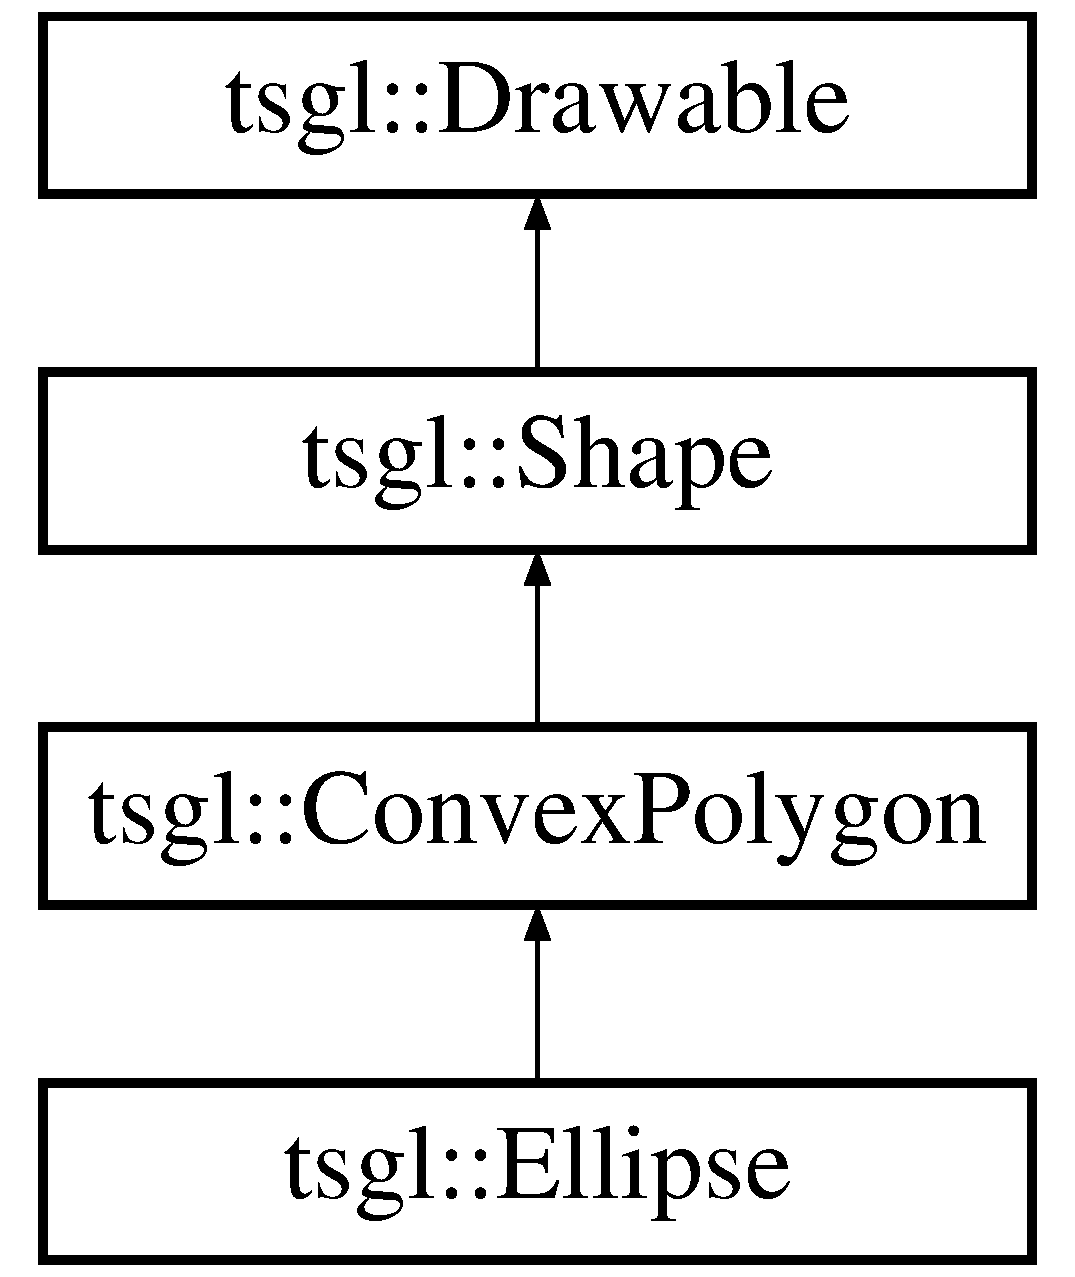
\includegraphics[height=4.000000cm]{classtsgl_1_1_ellipse}
\end{center}
\end{figure}
\subsection*{Public Member Functions}
\begin{DoxyCompactItemize}
\item 
\hyperlink{classtsgl_1_1_ellipse_a659436dbb6b37e117cbe98c3c7b23599}{Ellipse} (float x, float y, float z, G\+Lfloat x\+Radius, G\+Lfloat y\+Radius, float yaw, float pitch, float roll, \hyperlink{structtsgl_1_1_color_float}{Color\+Float} color)
\begin{DoxyCompactList}\small\item\em Explicitly constructs a new monocolored \hyperlink{classtsgl_1_1_ellipse}{Ellipse}. \end{DoxyCompactList}\item 
\hyperlink{classtsgl_1_1_ellipse_ac017f7eca9932720288bd261f4f1c9ba}{Ellipse} (float x, float y, float z, G\+Lfloat x\+Radius, G\+Lfloat y\+Radius, float yaw, float pitch, float roll, \hyperlink{structtsgl_1_1_color_float}{Color\+Float} color\mbox{[}$\,$\mbox{]})
\begin{DoxyCompactList}\small\item\em Explicitly constructs a new multicolored \hyperlink{classtsgl_1_1_ellipse}{Ellipse}. \end{DoxyCompactList}\item 
void \hyperlink{classtsgl_1_1_ellipse_a0bbb654f584ad6bb7a89c8fb6e1ecaf1}{set\+X\+Radius} (G\+Lfloat x\+Radius)
\begin{DoxyCompactList}\small\item\em Mutates the horizontal radius of the \hyperlink{classtsgl_1_1_ellipse}{Ellipse}. \end{DoxyCompactList}\item 
void \hyperlink{classtsgl_1_1_ellipse_aca11daaf59dd05b15943597a5f0adfd6}{set\+Y\+Radius} (G\+Lfloat y\+Radius)
\begin{DoxyCompactList}\small\item\em Mutates the vertical radius of the \hyperlink{classtsgl_1_1_ellipse}{Ellipse}. \end{DoxyCompactList}\item 
void \hyperlink{classtsgl_1_1_ellipse_aeee0a38af85a3d72ddef4d10579c2582}{change\+X\+Radius\+By} (G\+Lfloat delta)
\begin{DoxyCompactList}\small\item\em Mutates the horizontal radius of the \hyperlink{classtsgl_1_1_ellipse}{Ellipse} by the parameter amount. \end{DoxyCompactList}\item 
void \hyperlink{classtsgl_1_1_ellipse_a07c8ee9a4433de42a1b70f6a02385b91}{change\+Y\+Radius\+By} (G\+Lfloat delta)
\begin{DoxyCompactList}\small\item\em Mutates the vertical radius of the \hyperlink{classtsgl_1_1_ellipse}{Ellipse} by the parameter amount. \end{DoxyCompactList}\item 
G\+Lfloat \hyperlink{classtsgl_1_1_ellipse_ad3e100cf6e0cb429a3be1e5162c4aa61}{get\+X\+Radius} ()
\begin{DoxyCompactList}\small\item\em Accessor for the x-\/radius of the \hyperlink{classtsgl_1_1_ellipse}{Ellipse}. \end{DoxyCompactList}\item 
G\+Lfloat \hyperlink{classtsgl_1_1_ellipse_ab4371a2fae21b7fb874a4f5232e92f40}{get\+Y\+Radius} ()
\begin{DoxyCompactList}\small\item\em Accessor for the y-\/radius of the \hyperlink{classtsgl_1_1_ellipse}{Ellipse}. \end{DoxyCompactList}\item 
void \hyperlink{classtsgl_1_1_ellipse_afb71964e56fdd50e49ba46e8090aa858}{set\+Color} (\hyperlink{structtsgl_1_1_color_float}{Color\+Float} c)
\begin{DoxyCompactList}\small\item\em Sets the \hyperlink{classtsgl_1_1_shape}{Shape} to a new color. \end{DoxyCompactList}\item 
void \hyperlink{classtsgl_1_1_ellipse_a052ef5a609d7e8516d973ddc9e549c89}{set\+Color} (\hyperlink{structtsgl_1_1_color_float}{Color\+Float} c\mbox{[}$\,$\mbox{]})
\begin{DoxyCompactList}\small\item\em Sets the \hyperlink{classtsgl_1_1_ellipse}{Ellipse} to a new array of colors. \end{DoxyCompactList}\item 
virtual void \hyperlink{classtsgl_1_1_ellipse_a3d92da146589fc58112945daefafe98f}{get\+Colors} (std\+::vector$<$ \hyperlink{structtsgl_1_1_color_float}{Color\+Float} $>$ \&color\+Vec)
\begin{DoxyCompactList}\small\item\em Accessor for \hyperlink{classtsgl_1_1_ellipse}{Ellipse}\textquotesingle{}s colors. \end{DoxyCompactList}\end{DoxyCompactItemize}
\subsection*{Additional Inherited Members}


\subsection{Detailed Description}
Draw a simple ellipse. 

\hyperlink{classtsgl_1_1_ellipse}{Ellipse} is a class for holding vertex data for an ellipse. 

\subsection{Constructor \& Destructor Documentation}
\mbox{\Hypertarget{classtsgl_1_1_ellipse_a659436dbb6b37e117cbe98c3c7b23599}\label{classtsgl_1_1_ellipse_a659436dbb6b37e117cbe98c3c7b23599}} 
\index{tsgl\+::\+Ellipse@{tsgl\+::\+Ellipse}!Ellipse@{Ellipse}}
\index{Ellipse@{Ellipse}!tsgl\+::\+Ellipse@{tsgl\+::\+Ellipse}}
\subsubsection{\texorpdfstring{Ellipse()}{Ellipse()}\hspace{0.1cm}{\footnotesize\ttfamily [1/2]}}
{\footnotesize\ttfamily tsgl\+::\+Ellipse\+::\+Ellipse (\begin{DoxyParamCaption}\item[{float}]{x,  }\item[{float}]{y,  }\item[{float}]{z,  }\item[{G\+Lfloat}]{x\+Radius,  }\item[{G\+Lfloat}]{y\+Radius,  }\item[{float}]{yaw,  }\item[{float}]{pitch,  }\item[{float}]{roll,  }\item[{\hyperlink{structtsgl_1_1_color_float}{Color\+Float}}]{color }\end{DoxyParamCaption})}



Explicitly constructs a new monocolored \hyperlink{classtsgl_1_1_ellipse}{Ellipse}. 

This function draws a \hyperlink{classtsgl_1_1_ellipse}{Ellipse} with the given center, radii, rotation, and color. 
\begin{DoxyParams}{Parameters}
{\em x} & The x coordinate of the \hyperlink{classtsgl_1_1_ellipse}{Ellipse}\textquotesingle{}s center. \\
\hline
{\em y} & The y coordinate of the \hyperlink{classtsgl_1_1_ellipse}{Ellipse}\textquotesingle{}s center. \\
\hline
{\em z} & The z coordinate of the \hyperlink{classtsgl_1_1_ellipse}{Ellipse}\textquotesingle{}s center. \\
\hline
{\em x\+Radius} & The horizontal radius of the \hyperlink{classtsgl_1_1_ellipse}{Ellipse} in pixels. \\
\hline
{\em y\+Radius} & The vertical radius of the \hyperlink{classtsgl_1_1_ellipse}{Ellipse} in pixels. \\
\hline
{\em yaw} & The \hyperlink{classtsgl_1_1_ellipse}{Ellipse}\textquotesingle{}s yaw in 3D space. \\
\hline
{\em pitch} & The \hyperlink{classtsgl_1_1_ellipse}{Ellipse}\textquotesingle{}s pitch in 3D space. \\
\hline
{\em roll} & The \hyperlink{classtsgl_1_1_ellipse}{Ellipse}\textquotesingle{}s roll in 3D space. \\
\hline
{\em color} & The color of the \hyperlink{classtsgl_1_1_ellipse}{Ellipse}\textquotesingle{}s fill. \\
\hline
\end{DoxyParams}
\mbox{\Hypertarget{classtsgl_1_1_ellipse_ac017f7eca9932720288bd261f4f1c9ba}\label{classtsgl_1_1_ellipse_ac017f7eca9932720288bd261f4f1c9ba}} 
\index{tsgl\+::\+Ellipse@{tsgl\+::\+Ellipse}!Ellipse@{Ellipse}}
\index{Ellipse@{Ellipse}!tsgl\+::\+Ellipse@{tsgl\+::\+Ellipse}}
\subsubsection{\texorpdfstring{Ellipse()}{Ellipse()}\hspace{0.1cm}{\footnotesize\ttfamily [2/2]}}
{\footnotesize\ttfamily tsgl\+::\+Ellipse\+::\+Ellipse (\begin{DoxyParamCaption}\item[{float}]{x,  }\item[{float}]{y,  }\item[{float}]{z,  }\item[{G\+Lfloat}]{x\+Radius,  }\item[{G\+Lfloat}]{y\+Radius,  }\item[{float}]{yaw,  }\item[{float}]{pitch,  }\item[{float}]{roll,  }\item[{\hyperlink{structtsgl_1_1_color_float}{Color\+Float}}]{color\mbox{[}$\,$\mbox{]} }\end{DoxyParamCaption})}



Explicitly constructs a new multicolored \hyperlink{classtsgl_1_1_ellipse}{Ellipse}. 

This function draws a \hyperlink{classtsgl_1_1_ellipse}{Ellipse} with the given center, radii, rotation, and color. 
\begin{DoxyParams}{Parameters}
{\em x} & The x coordinate of the \hyperlink{classtsgl_1_1_ellipse}{Ellipse}\textquotesingle{}s center. \\
\hline
{\em y} & The y coordinate of the \hyperlink{classtsgl_1_1_ellipse}{Ellipse}\textquotesingle{}s center. \\
\hline
{\em z} & The z coordinate of the \hyperlink{classtsgl_1_1_ellipse}{Ellipse}\textquotesingle{}s center. \\
\hline
{\em x\+Radius} & The horizontal radius of the \hyperlink{classtsgl_1_1_ellipse}{Ellipse} in pixels. \\
\hline
{\em y\+Radius} & The vertical radius of the \hyperlink{classtsgl_1_1_ellipse}{Ellipse} in pixels. \\
\hline
{\em yaw} & The \hyperlink{classtsgl_1_1_ellipse}{Ellipse}\textquotesingle{}s yaw in 3D space. \\
\hline
{\em pitch} & The \hyperlink{classtsgl_1_1_ellipse}{Ellipse}\textquotesingle{}s pitch in 3D space. \\
\hline
{\em roll} & The \hyperlink{classtsgl_1_1_ellipse}{Ellipse}\textquotesingle{}s roll in 3D space. \\
\hline
{\em color} & An array of colors for the \hyperlink{classtsgl_1_1_ellipse}{Ellipse}\textquotesingle{}s fill. \\
\hline
\end{DoxyParams}


\subsection{Member Function Documentation}
\mbox{\Hypertarget{classtsgl_1_1_ellipse_aeee0a38af85a3d72ddef4d10579c2582}\label{classtsgl_1_1_ellipse_aeee0a38af85a3d72ddef4d10579c2582}} 
\index{tsgl\+::\+Ellipse@{tsgl\+::\+Ellipse}!change\+X\+Radius\+By@{change\+X\+Radius\+By}}
\index{change\+X\+Radius\+By@{change\+X\+Radius\+By}!tsgl\+::\+Ellipse@{tsgl\+::\+Ellipse}}
\subsubsection{\texorpdfstring{change\+X\+Radius\+By()}{changeXRadiusBy()}}
{\footnotesize\ttfamily void tsgl\+::\+Ellipse\+::change\+X\+Radius\+By (\begin{DoxyParamCaption}\item[{G\+Lfloat}]{delta }\end{DoxyParamCaption})}



Mutates the horizontal radius of the \hyperlink{classtsgl_1_1_ellipse}{Ellipse} by the parameter amount. 


\begin{DoxyParams}{Parameters}
{\em delta} & The amount by which to change the x-\/radius of the \hyperlink{classtsgl_1_1_ellipse}{Ellipse}. \\
\hline
\end{DoxyParams}
\mbox{\Hypertarget{classtsgl_1_1_ellipse_a07c8ee9a4433de42a1b70f6a02385b91}\label{classtsgl_1_1_ellipse_a07c8ee9a4433de42a1b70f6a02385b91}} 
\index{tsgl\+::\+Ellipse@{tsgl\+::\+Ellipse}!change\+Y\+Radius\+By@{change\+Y\+Radius\+By}}
\index{change\+Y\+Radius\+By@{change\+Y\+Radius\+By}!tsgl\+::\+Ellipse@{tsgl\+::\+Ellipse}}
\subsubsection{\texorpdfstring{change\+Y\+Radius\+By()}{changeYRadiusBy()}}
{\footnotesize\ttfamily void tsgl\+::\+Ellipse\+::change\+Y\+Radius\+By (\begin{DoxyParamCaption}\item[{G\+Lfloat}]{delta }\end{DoxyParamCaption})}



Mutates the vertical radius of the \hyperlink{classtsgl_1_1_ellipse}{Ellipse} by the parameter amount. 


\begin{DoxyParams}{Parameters}
{\em delta} & The amount by which to change the y-\/radius of the \hyperlink{classtsgl_1_1_ellipse}{Ellipse}. \\
\hline
\end{DoxyParams}
\mbox{\Hypertarget{classtsgl_1_1_ellipse_a3d92da146589fc58112945daefafe98f}\label{classtsgl_1_1_ellipse_a3d92da146589fc58112945daefafe98f}} 
\index{tsgl\+::\+Ellipse@{tsgl\+::\+Ellipse}!get\+Colors@{get\+Colors}}
\index{get\+Colors@{get\+Colors}!tsgl\+::\+Ellipse@{tsgl\+::\+Ellipse}}
\subsubsection{\texorpdfstring{get\+Colors()}{getColors()}}
{\footnotesize\ttfamily void tsgl\+::\+Ellipse\+::get\+Colors (\begin{DoxyParamCaption}\item[{std\+::vector$<$ \hyperlink{structtsgl_1_1_color_float}{Color\+Float} $>$ \&}]{color\+Vec }\end{DoxyParamCaption})\hspace{0.3cm}{\ttfamily [virtual]}}



Accessor for \hyperlink{classtsgl_1_1_ellipse}{Ellipse}\textquotesingle{}s colors. 

Populates the reference parameter vector with a \hyperlink{structtsgl_1_1_color_float}{Color\+Float} for each section of \hyperlink{classtsgl_1_1_ellipse}{Ellipse}. 
\begin{DoxyParams}{Parameters}
{\em color\+Vec} & A vector of Color\+Floats to which the Color\+Floats associated with \hyperlink{classtsgl_1_1_ellipse}{Ellipse} will be pushed. \\
\hline
\end{DoxyParams}
\begin{DoxyNote}{Note}
Overrides \hyperlink{classtsgl_1_1_shape_a6f54fe4d049f69a287edf8335a9509f8}{Shape\+::get\+Colors()}. 
\end{DoxyNote}


Reimplemented from \hyperlink{classtsgl_1_1_shape_a6f54fe4d049f69a287edf8335a9509f8}{tsgl\+::\+Shape}.



Referenced by set\+Color().

\mbox{\Hypertarget{classtsgl_1_1_ellipse_ad3e100cf6e0cb429a3be1e5162c4aa61}\label{classtsgl_1_1_ellipse_ad3e100cf6e0cb429a3be1e5162c4aa61}} 
\index{tsgl\+::\+Ellipse@{tsgl\+::\+Ellipse}!get\+X\+Radius@{get\+X\+Radius}}
\index{get\+X\+Radius@{get\+X\+Radius}!tsgl\+::\+Ellipse@{tsgl\+::\+Ellipse}}
\subsubsection{\texorpdfstring{get\+X\+Radius()}{getXRadius()}}
{\footnotesize\ttfamily G\+Lfloat tsgl\+::\+Ellipse\+::get\+X\+Radius (\begin{DoxyParamCaption}{ }\end{DoxyParamCaption})\hspace{0.3cm}{\ttfamily [inline]}}



Accessor for the x-\/radius of the \hyperlink{classtsgl_1_1_ellipse}{Ellipse}. 

Returns the value of the my\+X\+Radius private variable, a G\+Lfloat. \mbox{\Hypertarget{classtsgl_1_1_ellipse_ab4371a2fae21b7fb874a4f5232e92f40}\label{classtsgl_1_1_ellipse_ab4371a2fae21b7fb874a4f5232e92f40}} 
\index{tsgl\+::\+Ellipse@{tsgl\+::\+Ellipse}!get\+Y\+Radius@{get\+Y\+Radius}}
\index{get\+Y\+Radius@{get\+Y\+Radius}!tsgl\+::\+Ellipse@{tsgl\+::\+Ellipse}}
\subsubsection{\texorpdfstring{get\+Y\+Radius()}{getYRadius()}}
{\footnotesize\ttfamily G\+Lfloat tsgl\+::\+Ellipse\+::get\+Y\+Radius (\begin{DoxyParamCaption}{ }\end{DoxyParamCaption})\hspace{0.3cm}{\ttfamily [inline]}}



Accessor for the y-\/radius of the \hyperlink{classtsgl_1_1_ellipse}{Ellipse}. 

Returns the value of the my\+Y\+Radius private variable, a G\+Lfloat. \mbox{\Hypertarget{classtsgl_1_1_ellipse_afb71964e56fdd50e49ba46e8090aa858}\label{classtsgl_1_1_ellipse_afb71964e56fdd50e49ba46e8090aa858}} 
\index{tsgl\+::\+Ellipse@{tsgl\+::\+Ellipse}!set\+Color@{set\+Color}}
\index{set\+Color@{set\+Color}!tsgl\+::\+Ellipse@{tsgl\+::\+Ellipse}}
\subsubsection{\texorpdfstring{set\+Color()}{setColor()}\hspace{0.1cm}{\footnotesize\ttfamily [1/2]}}
{\footnotesize\ttfamily void tsgl\+::\+Ellipse\+::set\+Color (\begin{DoxyParamCaption}\item[{\hyperlink{structtsgl_1_1_color_float}{Color\+Float}}]{c }\end{DoxyParamCaption})\hspace{0.3cm}{\ttfamily [inline]}, {\ttfamily [virtual]}}



Sets the \hyperlink{classtsgl_1_1_shape}{Shape} to a new color. 


\begin{DoxyParams}{Parameters}
{\em c} & The new \hyperlink{structtsgl_1_1_color_float}{Color\+Float}. \\
\hline
\end{DoxyParams}


Reimplemented from \hyperlink{classtsgl_1_1_shape_abdb01321cddfd2db1481eefbc2836f70}{tsgl\+::\+Shape}.

\mbox{\Hypertarget{classtsgl_1_1_ellipse_a052ef5a609d7e8516d973ddc9e549c89}\label{classtsgl_1_1_ellipse_a052ef5a609d7e8516d973ddc9e549c89}} 
\index{tsgl\+::\+Ellipse@{tsgl\+::\+Ellipse}!set\+Color@{set\+Color}}
\index{set\+Color@{set\+Color}!tsgl\+::\+Ellipse@{tsgl\+::\+Ellipse}}
\subsubsection{\texorpdfstring{set\+Color()}{setColor()}\hspace{0.1cm}{\footnotesize\ttfamily [2/2]}}
{\footnotesize\ttfamily void tsgl\+::\+Ellipse\+::set\+Color (\begin{DoxyParamCaption}\item[{\hyperlink{structtsgl_1_1_color_float}{Color\+Float}}]{c\mbox{[}$\,$\mbox{]} }\end{DoxyParamCaption})\hspace{0.3cm}{\ttfamily [virtual]}}



Sets the \hyperlink{classtsgl_1_1_ellipse}{Ellipse} to a new array of colors. 


\begin{DoxyParams}{Parameters}
{\em c} & An array of the new Color\+Floats. \\
\hline
\end{DoxyParams}


Reimplemented from \hyperlink{classtsgl_1_1_shape_ad7e554b5d4cea111ec518548b9f21388}{tsgl\+::\+Shape}.

\mbox{\Hypertarget{classtsgl_1_1_ellipse_a0bbb654f584ad6bb7a89c8fb6e1ecaf1}\label{classtsgl_1_1_ellipse_a0bbb654f584ad6bb7a89c8fb6e1ecaf1}} 
\index{tsgl\+::\+Ellipse@{tsgl\+::\+Ellipse}!set\+X\+Radius@{set\+X\+Radius}}
\index{set\+X\+Radius@{set\+X\+Radius}!tsgl\+::\+Ellipse@{tsgl\+::\+Ellipse}}
\subsubsection{\texorpdfstring{set\+X\+Radius()}{setXRadius()}}
{\footnotesize\ttfamily void tsgl\+::\+Ellipse\+::set\+X\+Radius (\begin{DoxyParamCaption}\item[{G\+Lfloat}]{x\+Radius }\end{DoxyParamCaption})}



Mutates the horizontal radius of the \hyperlink{classtsgl_1_1_ellipse}{Ellipse}. 


\begin{DoxyParams}{Parameters}
{\em x\+Radius} & The \hyperlink{classtsgl_1_1_ellipse}{Ellipse}\textquotesingle{}s new x-\/radius. \\
\hline
\end{DoxyParams}
\mbox{\Hypertarget{classtsgl_1_1_ellipse_aca11daaf59dd05b15943597a5f0adfd6}\label{classtsgl_1_1_ellipse_aca11daaf59dd05b15943597a5f0adfd6}} 
\index{tsgl\+::\+Ellipse@{tsgl\+::\+Ellipse}!set\+Y\+Radius@{set\+Y\+Radius}}
\index{set\+Y\+Radius@{set\+Y\+Radius}!tsgl\+::\+Ellipse@{tsgl\+::\+Ellipse}}
\subsubsection{\texorpdfstring{set\+Y\+Radius()}{setYRadius()}}
{\footnotesize\ttfamily void tsgl\+::\+Ellipse\+::set\+Y\+Radius (\begin{DoxyParamCaption}\item[{G\+Lfloat}]{y\+Radius }\end{DoxyParamCaption})}



Mutates the vertical radius of the \hyperlink{classtsgl_1_1_ellipse}{Ellipse}. 


\begin{DoxyParams}{Parameters}
{\em Y\+Radius} & The \hyperlink{classtsgl_1_1_ellipse}{Ellipse}\textquotesingle{}s new y-\/radius. \\
\hline
\end{DoxyParams}


The documentation for this class was generated from the following files\+:\begin{DoxyCompactItemize}
\item 
Ellipse.\+h\item 
Ellipse.\+cpp\end{DoxyCompactItemize}

\hypertarget{classtsgl_1_1_ellipsoid}{}\section{tsgl\+:\+:Ellipsoid Class Reference}
\label{classtsgl_1_1_ellipsoid}\index{tsgl\+::\+Ellipsoid@{tsgl\+::\+Ellipsoid}}


Draw an arbitrary \hyperlink{classtsgl_1_1_ellipsoid}{Ellipsoid} with colored vertices.  




{\ttfamily \#include $<$Ellipsoid.\+h$>$}

Inheritance diagram for tsgl\+:\+:Ellipsoid\+:\begin{figure}[H]
\begin{center}
\leavevmode
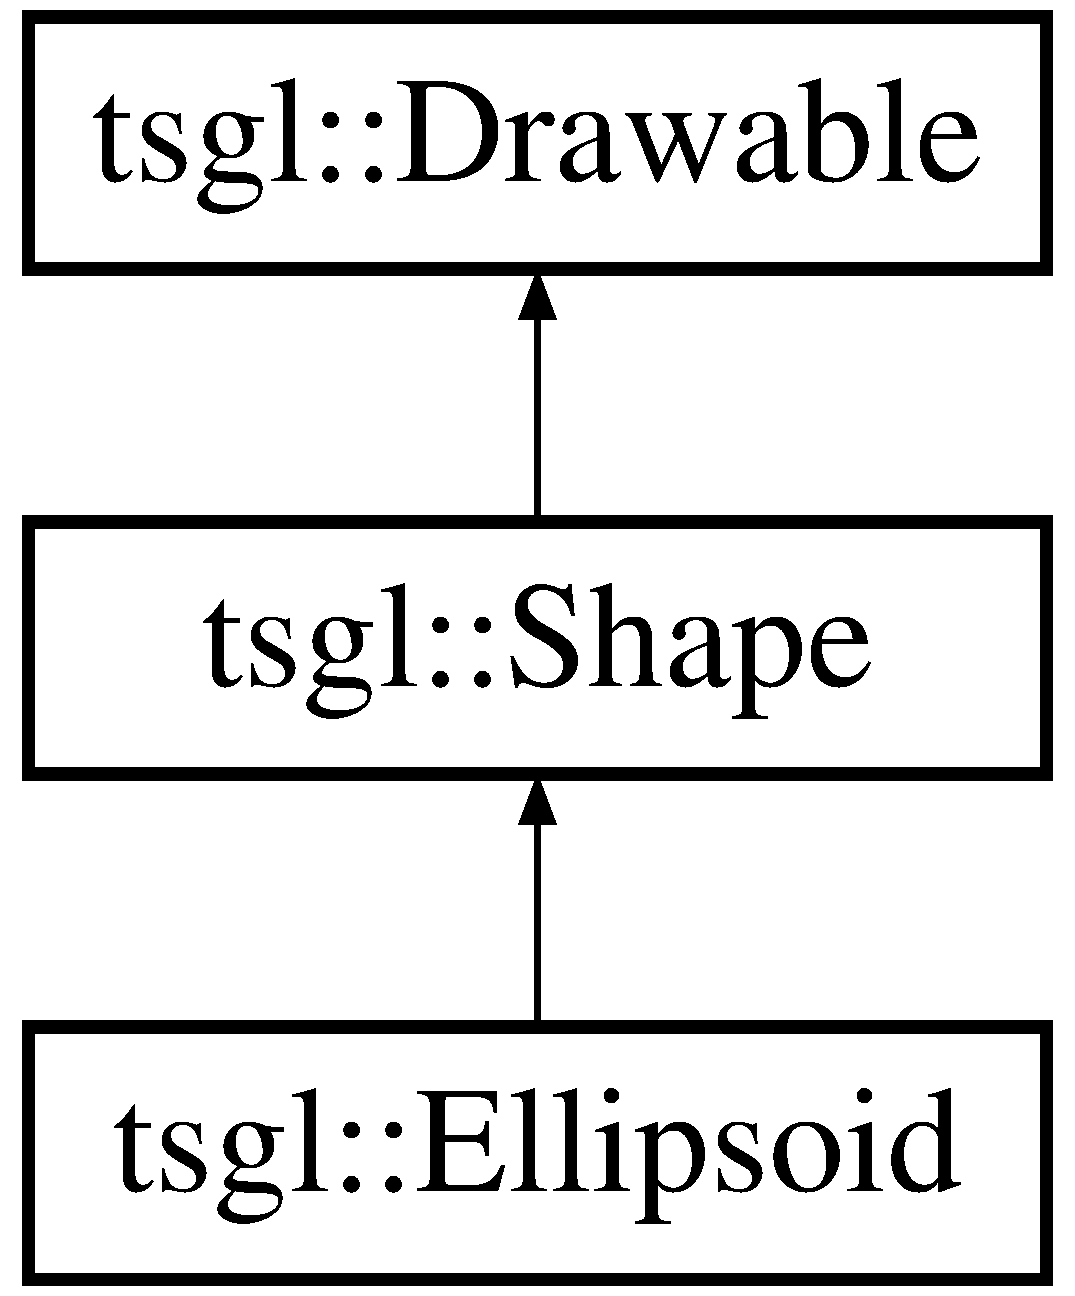
\includegraphics[height=3.000000cm]{classtsgl_1_1_ellipsoid}
\end{center}
\end{figure}
\subsection*{Public Member Functions}
\begin{DoxyCompactItemize}
\item 
\hyperlink{classtsgl_1_1_ellipsoid_afd749d93e94a1d0310fb64e01d348cec}{Ellipsoid} (float x, float y, float z, G\+Lfloat x\+Radius, G\+Lfloat y\+Radius, G\+Lfloat z\+Radius, float yaw, float pitch, float roll, \hyperlink{structtsgl_1_1_color_float}{Color\+Float} c)
\begin{DoxyCompactList}\small\item\em Explicitly constructs a new \hyperlink{classtsgl_1_1_ellipsoid}{Ellipsoid}. \end{DoxyCompactList}\item 
\hyperlink{classtsgl_1_1_ellipsoid_a7e1a2eaf27ee32aeaf6415cb6b4eb149}{Ellipsoid} (float x, float y, float z, G\+Lfloat x\+Radius, G\+Lfloat y\+Radius, G\+Lfloat z\+Radius, float yaw, float pitch, float roll, \hyperlink{structtsgl_1_1_color_float}{Color\+Float} c\mbox{[}$\,$\mbox{]})
\begin{DoxyCompactList}\small\item\em Explicitly constructs a new \hyperlink{classtsgl_1_1_ellipsoid}{Ellipsoid}. \end{DoxyCompactList}\item 
virtual void \hyperlink{classtsgl_1_1_ellipsoid_a5ddfa2710dfff0e34186a9719f058fb7}{set\+X\+Radius} (G\+Lfloat radiusX)
\begin{DoxyCompactList}\small\item\em Mutates the \hyperlink{classtsgl_1_1_ellipsoid}{Ellipsoid}\textquotesingle{}s x-\/axis radius. \end{DoxyCompactList}\item 
virtual void \hyperlink{classtsgl_1_1_ellipsoid_ab0db918041ca4638236b007dade3cff0}{change\+X\+Radius\+By} (G\+Lfloat delta)
\begin{DoxyCompactList}\small\item\em Mutates the \hyperlink{classtsgl_1_1_ellipsoid}{Ellipsoid}\textquotesingle{}s x-\/axis radius by the parameter amount. \end{DoxyCompactList}\item 
virtual void \hyperlink{classtsgl_1_1_ellipsoid_a6a47161df73d22188aae92016c3058ca}{set\+Y\+Radius} (G\+Lfloat radiusY)
\begin{DoxyCompactList}\small\item\em Mutates the \hyperlink{classtsgl_1_1_ellipsoid}{Ellipsoid}\textquotesingle{}s y-\/axis radius. \end{DoxyCompactList}\item 
virtual void \hyperlink{classtsgl_1_1_ellipsoid_a84f0a1161d9047e5661de030ed924d38}{change\+Y\+Radius\+By} (G\+Lfloat delta)
\begin{DoxyCompactList}\small\item\em Mutates the \hyperlink{classtsgl_1_1_ellipsoid}{Ellipsoid}\textquotesingle{}s y-\/axis radius by the parameter amount. \end{DoxyCompactList}\item 
virtual void \hyperlink{classtsgl_1_1_ellipsoid_a6663042d8935a658b8a27a5843d897e8}{set\+Z\+Radius} (G\+Lfloat radiusZ)
\begin{DoxyCompactList}\small\item\em Mutates the \hyperlink{classtsgl_1_1_ellipsoid}{Ellipsoid}\textquotesingle{}s z-\/axis radius. \end{DoxyCompactList}\item 
virtual void \hyperlink{classtsgl_1_1_ellipsoid_a1e749caabe1c994404027c9d78098356}{change\+Z\+Radius\+By} (G\+Lfloat delta)
\begin{DoxyCompactList}\small\item\em Mutates the \hyperlink{classtsgl_1_1_ellipsoid}{Ellipsoid}\textquotesingle{}s z-\/axis radius by the parameter amount. \end{DoxyCompactList}\item 
\mbox{\Hypertarget{classtsgl_1_1_ellipsoid_a8231ebee8fb2b791679dc1ffae36f238}\label{classtsgl_1_1_ellipsoid_a8231ebee8fb2b791679dc1ffae36f238}} 
virtual G\+Lfloat {\bfseries get\+X\+Radius} ()
\item 
\mbox{\Hypertarget{classtsgl_1_1_ellipsoid_a0f0537cbd8feb6b68d60ddc3a08ec75d}\label{classtsgl_1_1_ellipsoid_a0f0537cbd8feb6b68d60ddc3a08ec75d}} 
virtual G\+Lfloat {\bfseries get\+Y\+Radius} ()
\item 
\mbox{\Hypertarget{classtsgl_1_1_ellipsoid_aff43989fc02b3a833014ee426778752b}\label{classtsgl_1_1_ellipsoid_aff43989fc02b3a833014ee426778752b}} 
virtual G\+Lfloat {\bfseries get\+Z\+Radius} ()
\item 
virtual void \hyperlink{classtsgl_1_1_ellipsoid_afc2fc98057e5d19d8fa0c45f07273cdb}{set\+Color} (\hyperlink{structtsgl_1_1_color_float}{Color\+Float} c)
\begin{DoxyCompactList}\small\item\em Sets the \hyperlink{classtsgl_1_1_ellipsoid}{Ellipsoid} to a new color. \end{DoxyCompactList}\item 
virtual void \hyperlink{classtsgl_1_1_ellipsoid_ab8e15e879521e4c96be8192258cad26e}{set\+Color} (\hyperlink{structtsgl_1_1_color_float}{Color\+Float} c\mbox{[}$\,$\mbox{]})
\begin{DoxyCompactList}\small\item\em Sets the \hyperlink{classtsgl_1_1_ellipsoid}{Ellipsoid} to an array of new colors. \end{DoxyCompactList}\item 
virtual void \hyperlink{classtsgl_1_1_ellipsoid_ac5c9278659df646c17ef4172e13c7cb3}{get\+Colors} (std\+::vector$<$ \hyperlink{structtsgl_1_1_color_float}{Color\+Float} $>$ \&color\+Vec)
\begin{DoxyCompactList}\small\item\em Accessor for \hyperlink{classtsgl_1_1_ellipsoid}{Ellipsoid}\textquotesingle{}s colors. \end{DoxyCompactList}\end{DoxyCompactItemize}
\subsection*{Protected Attributes}
\begin{DoxyCompactItemize}
\item 
\mbox{\Hypertarget{classtsgl_1_1_ellipsoid_a065322fb3c3c07b1ed90ff7f5adaca0d}\label{classtsgl_1_1_ellipsoid_a065322fb3c3c07b1ed90ff7f5adaca0d}} 
G\+Lfloat {\bfseries my\+X\+Radius}
\item 
\mbox{\Hypertarget{classtsgl_1_1_ellipsoid_a331185ad15cd3cad43dd46c1633feb97}\label{classtsgl_1_1_ellipsoid_a331185ad15cd3cad43dd46c1633feb97}} 
G\+Lfloat {\bfseries my\+Y\+Radius}
\item 
\mbox{\Hypertarget{classtsgl_1_1_ellipsoid_af908c43416a1f58b5aa8c2922fdcfe57}\label{classtsgl_1_1_ellipsoid_af908c43416a1f58b5aa8c2922fdcfe57}} 
G\+Lfloat {\bfseries my\+Z\+Radius}
\item 
\mbox{\Hypertarget{classtsgl_1_1_ellipsoid_aebaa7282129758fdf7e16e4aae03049b}\label{classtsgl_1_1_ellipsoid_aebaa7282129758fdf7e16e4aae03049b}} 
int {\bfseries horizontal\+Sections}
\item 
\mbox{\Hypertarget{classtsgl_1_1_ellipsoid_ac863721eb739dd9c3a125ee0f63d3d7b}\label{classtsgl_1_1_ellipsoid_ac863721eb739dd9c3a125ee0f63d3d7b}} 
int {\bfseries vertical\+Sections}
\end{DoxyCompactItemize}
\subsection*{Additional Inherited Members}


\subsection{Detailed Description}
Draw an arbitrary \hyperlink{classtsgl_1_1_ellipsoid}{Ellipsoid} with colored vertices. 

\hyperlink{classtsgl_1_1_ellipsoid}{Ellipsoid} is a class for holding vertex data for an \hyperlink{classtsgl_1_1_ellipsoid}{Ellipsoid}. 

\subsection{Constructor \& Destructor Documentation}
\mbox{\Hypertarget{classtsgl_1_1_ellipsoid_afd749d93e94a1d0310fb64e01d348cec}\label{classtsgl_1_1_ellipsoid_afd749d93e94a1d0310fb64e01d348cec}} 
\index{tsgl\+::\+Ellipsoid@{tsgl\+::\+Ellipsoid}!Ellipsoid@{Ellipsoid}}
\index{Ellipsoid@{Ellipsoid}!tsgl\+::\+Ellipsoid@{tsgl\+::\+Ellipsoid}}
\subsubsection{\texorpdfstring{Ellipsoid()}{Ellipsoid()}\hspace{0.1cm}{\footnotesize\ttfamily [1/2]}}
{\footnotesize\ttfamily tsgl\+::\+Ellipsoid\+::\+Ellipsoid (\begin{DoxyParamCaption}\item[{float}]{x,  }\item[{float}]{y,  }\item[{float}]{z,  }\item[{G\+Lfloat}]{x\+Radius,  }\item[{G\+Lfloat}]{y\+Radius,  }\item[{G\+Lfloat}]{z\+Radius,  }\item[{float}]{yaw,  }\item[{float}]{pitch,  }\item[{float}]{roll,  }\item[{\hyperlink{structtsgl_1_1_color_float}{Color\+Float}}]{c }\end{DoxyParamCaption})}



Explicitly constructs a new \hyperlink{classtsgl_1_1_ellipsoid}{Ellipsoid}. 

Explicit constructor for a \hyperlink{classtsgl_1_1_ellipsoid}{Ellipsoid} object. 
\begin{DoxyParams}{Parameters}
{\em x} & The x coordinate of the center of the \hyperlink{classtsgl_1_1_ellipsoid}{Ellipsoid}. \\
\hline
{\em y} & The y coordinate of the center of the \hyperlink{classtsgl_1_1_ellipsoid}{Ellipsoid}. \\
\hline
{\em z} & The z coordinate of the center of the \hyperlink{classtsgl_1_1_ellipsoid}{Ellipsoid}. \\
\hline
{\em x\+Radius} & The \hyperlink{classtsgl_1_1_ellipsoid}{Ellipsoid}\textquotesingle{}s radius on the x-\/axis. \\
\hline
{\em y\+Radius} & The \hyperlink{classtsgl_1_1_ellipsoid}{Ellipsoid}\textquotesingle{}s radius on the y-\/axis. \\
\hline
{\em z\+Radius} & The \hyperlink{classtsgl_1_1_ellipsoid}{Ellipsoid}\textquotesingle{}s radius on the z-\/axis. \\
\hline
{\em yaw} & The \hyperlink{classtsgl_1_1_ellipsoid}{Ellipsoid}\textquotesingle{}s yaw. \\
\hline
{\em pitch} & The \hyperlink{classtsgl_1_1_ellipsoid}{Ellipsoid}\textquotesingle{}s pitch. \\
\hline
{\em roll} & The \hyperlink{classtsgl_1_1_ellipsoid}{Ellipsoid}\textquotesingle{}s roll. \\
\hline
{\em c} & A \hyperlink{structtsgl_1_1_color_float}{Color\+Float} for the \hyperlink{classtsgl_1_1_ellipsoid}{Ellipsoid}\textquotesingle{}s vertex colors. \\
\hline
\end{DoxyParams}
\begin{DoxyWarning}{Warning}
An invariant is held where if any radius isn\textquotesingle{}t positive then an error message is given. 
\end{DoxyWarning}
\begin{DoxyReturn}{Returns}
A new \hyperlink{classtsgl_1_1_ellipsoid}{Ellipsoid} with a buffer for storing the specified numbered of vertices. 
\end{DoxyReturn}
\mbox{\Hypertarget{classtsgl_1_1_ellipsoid_a7e1a2eaf27ee32aeaf6415cb6b4eb149}\label{classtsgl_1_1_ellipsoid_a7e1a2eaf27ee32aeaf6415cb6b4eb149}} 
\index{tsgl\+::\+Ellipsoid@{tsgl\+::\+Ellipsoid}!Ellipsoid@{Ellipsoid}}
\index{Ellipsoid@{Ellipsoid}!tsgl\+::\+Ellipsoid@{tsgl\+::\+Ellipsoid}}
\subsubsection{\texorpdfstring{Ellipsoid()}{Ellipsoid()}\hspace{0.1cm}{\footnotesize\ttfamily [2/2]}}
{\footnotesize\ttfamily tsgl\+::\+Ellipsoid\+::\+Ellipsoid (\begin{DoxyParamCaption}\item[{float}]{x,  }\item[{float}]{y,  }\item[{float}]{z,  }\item[{G\+Lfloat}]{x\+Radius,  }\item[{G\+Lfloat}]{y\+Radius,  }\item[{G\+Lfloat}]{z\+Radius,  }\item[{float}]{yaw,  }\item[{float}]{pitch,  }\item[{float}]{roll,  }\item[{\hyperlink{structtsgl_1_1_color_float}{Color\+Float}}]{c\mbox{[}$\,$\mbox{]} }\end{DoxyParamCaption})}



Explicitly constructs a new \hyperlink{classtsgl_1_1_ellipsoid}{Ellipsoid}. 

Explicit constructor for a \hyperlink{classtsgl_1_1_ellipsoid}{Ellipsoid} object. 
\begin{DoxyParams}{Parameters}
{\em x} & The x coordinate of the center of the \hyperlink{classtsgl_1_1_ellipsoid}{Ellipsoid}. \\
\hline
{\em y} & The y coordinate of the center of the \hyperlink{classtsgl_1_1_ellipsoid}{Ellipsoid}. \\
\hline
{\em z} & The z coordinate of the center of the \hyperlink{classtsgl_1_1_ellipsoid}{Ellipsoid}. \\
\hline
{\em x\+Radius} & The \hyperlink{classtsgl_1_1_ellipsoid}{Ellipsoid}\textquotesingle{}s radius on the x-\/axis. \\
\hline
{\em y\+Radius} & The \hyperlink{classtsgl_1_1_ellipsoid}{Ellipsoid}\textquotesingle{}s radius on the y-\/axis. \\
\hline
{\em z\+Radius} & The \hyperlink{classtsgl_1_1_ellipsoid}{Ellipsoid}\textquotesingle{}s radius on the z-\/axis. \\
\hline
{\em yaw} & The \hyperlink{classtsgl_1_1_ellipsoid}{Ellipsoid}\textquotesingle{}s yaw. \\
\hline
{\em pitch} & The \hyperlink{classtsgl_1_1_ellipsoid}{Ellipsoid}\textquotesingle{}s pitch. \\
\hline
{\em roll} & The \hyperlink{classtsgl_1_1_ellipsoid}{Ellipsoid}\textquotesingle{}s roll. \\
\hline
{\em c} & An array of Color\+Floats for the \hyperlink{classtsgl_1_1_ellipsoid}{Ellipsoid}\textquotesingle{}s vertex colors. \\
\hline
\end{DoxyParams}
\begin{DoxyWarning}{Warning}
An invariant is held where if any radius isn\textquotesingle{}t positive then an error message is given. 
\end{DoxyWarning}
\begin{DoxyReturn}{Returns}
A new \hyperlink{classtsgl_1_1_ellipsoid}{Ellipsoid} with a buffer for storing the specified numbered of vertices. 
\end{DoxyReturn}


\subsection{Member Function Documentation}
\mbox{\Hypertarget{classtsgl_1_1_ellipsoid_ab0db918041ca4638236b007dade3cff0}\label{classtsgl_1_1_ellipsoid_ab0db918041ca4638236b007dade3cff0}} 
\index{tsgl\+::\+Ellipsoid@{tsgl\+::\+Ellipsoid}!change\+X\+Radius\+By@{change\+X\+Radius\+By}}
\index{change\+X\+Radius\+By@{change\+X\+Radius\+By}!tsgl\+::\+Ellipsoid@{tsgl\+::\+Ellipsoid}}
\subsubsection{\texorpdfstring{change\+X\+Radius\+By()}{changeXRadiusBy()}}
{\footnotesize\ttfamily void tsgl\+::\+Ellipsoid\+::change\+X\+Radius\+By (\begin{DoxyParamCaption}\item[{G\+Lfloat}]{delta }\end{DoxyParamCaption})\hspace{0.3cm}{\ttfamily [virtual]}}



Mutates the \hyperlink{classtsgl_1_1_ellipsoid}{Ellipsoid}\textquotesingle{}s x-\/axis radius by the parameter amount. 


\begin{DoxyParams}{Parameters}
{\em delta} & The amount by which to change the x-\/axis radius of the \hyperlink{classtsgl_1_1_ellipsoid}{Ellipsoid}. \\
\hline
\end{DoxyParams}
\mbox{\Hypertarget{classtsgl_1_1_ellipsoid_a84f0a1161d9047e5661de030ed924d38}\label{classtsgl_1_1_ellipsoid_a84f0a1161d9047e5661de030ed924d38}} 
\index{tsgl\+::\+Ellipsoid@{tsgl\+::\+Ellipsoid}!change\+Y\+Radius\+By@{change\+Y\+Radius\+By}}
\index{change\+Y\+Radius\+By@{change\+Y\+Radius\+By}!tsgl\+::\+Ellipsoid@{tsgl\+::\+Ellipsoid}}
\subsubsection{\texorpdfstring{change\+Y\+Radius\+By()}{changeYRadiusBy()}}
{\footnotesize\ttfamily void tsgl\+::\+Ellipsoid\+::change\+Y\+Radius\+By (\begin{DoxyParamCaption}\item[{G\+Lfloat}]{delta }\end{DoxyParamCaption})\hspace{0.3cm}{\ttfamily [virtual]}}



Mutates the \hyperlink{classtsgl_1_1_ellipsoid}{Ellipsoid}\textquotesingle{}s y-\/axis radius by the parameter amount. 


\begin{DoxyParams}{Parameters}
{\em delta} & The amount by which to change the y-\/axis radius of the \hyperlink{classtsgl_1_1_ellipsoid}{Ellipsoid}. \\
\hline
\end{DoxyParams}
\mbox{\Hypertarget{classtsgl_1_1_ellipsoid_a1e749caabe1c994404027c9d78098356}\label{classtsgl_1_1_ellipsoid_a1e749caabe1c994404027c9d78098356}} 
\index{tsgl\+::\+Ellipsoid@{tsgl\+::\+Ellipsoid}!change\+Z\+Radius\+By@{change\+Z\+Radius\+By}}
\index{change\+Z\+Radius\+By@{change\+Z\+Radius\+By}!tsgl\+::\+Ellipsoid@{tsgl\+::\+Ellipsoid}}
\subsubsection{\texorpdfstring{change\+Z\+Radius\+By()}{changeZRadiusBy()}}
{\footnotesize\ttfamily void tsgl\+::\+Ellipsoid\+::change\+Z\+Radius\+By (\begin{DoxyParamCaption}\item[{G\+Lfloat}]{delta }\end{DoxyParamCaption})\hspace{0.3cm}{\ttfamily [virtual]}}



Mutates the \hyperlink{classtsgl_1_1_ellipsoid}{Ellipsoid}\textquotesingle{}s z-\/axis radius by the parameter amount. 


\begin{DoxyParams}{Parameters}
{\em delta} & The amount by which to change the z-\/axis radius of the \hyperlink{classtsgl_1_1_ellipsoid}{Ellipsoid}. \\
\hline
\end{DoxyParams}
\mbox{\Hypertarget{classtsgl_1_1_ellipsoid_ac5c9278659df646c17ef4172e13c7cb3}\label{classtsgl_1_1_ellipsoid_ac5c9278659df646c17ef4172e13c7cb3}} 
\index{tsgl\+::\+Ellipsoid@{tsgl\+::\+Ellipsoid}!get\+Colors@{get\+Colors}}
\index{get\+Colors@{get\+Colors}!tsgl\+::\+Ellipsoid@{tsgl\+::\+Ellipsoid}}
\subsubsection{\texorpdfstring{get\+Colors()}{getColors()}}
{\footnotesize\ttfamily void tsgl\+::\+Ellipsoid\+::get\+Colors (\begin{DoxyParamCaption}\item[{std\+::vector$<$ \hyperlink{structtsgl_1_1_color_float}{Color\+Float} $>$ \&}]{color\+Vec }\end{DoxyParamCaption})\hspace{0.3cm}{\ttfamily [virtual]}}



Accessor for \hyperlink{classtsgl_1_1_ellipsoid}{Ellipsoid}\textquotesingle{}s colors. 

Populates the reference parameter vector with a \hyperlink{structtsgl_1_1_color_float}{Color\+Float} for each section of \hyperlink{classtsgl_1_1_ellipsoid}{Ellipsoid}. 
\begin{DoxyParams}{Parameters}
{\em color\+Vec} & A vector of Color\+Floats to which the Color\+Floats associated with \hyperlink{classtsgl_1_1_ellipsoid}{Ellipsoid} will be pushed. \\
\hline
\end{DoxyParams}
\begin{DoxyNote}{Note}
Overrides \hyperlink{classtsgl_1_1_shape_a6f54fe4d049f69a287edf8335a9509f8}{Shape\+::get\+Colors()}. 
\end{DoxyNote}


Reimplemented from \hyperlink{classtsgl_1_1_shape_a6f54fe4d049f69a287edf8335a9509f8}{tsgl\+::\+Shape}.

\mbox{\Hypertarget{classtsgl_1_1_ellipsoid_afc2fc98057e5d19d8fa0c45f07273cdb}\label{classtsgl_1_1_ellipsoid_afc2fc98057e5d19d8fa0c45f07273cdb}} 
\index{tsgl\+::\+Ellipsoid@{tsgl\+::\+Ellipsoid}!set\+Color@{set\+Color}}
\index{set\+Color@{set\+Color}!tsgl\+::\+Ellipsoid@{tsgl\+::\+Ellipsoid}}
\subsubsection{\texorpdfstring{set\+Color()}{setColor()}\hspace{0.1cm}{\footnotesize\ttfamily [1/2]}}
{\footnotesize\ttfamily void tsgl\+::\+Ellipsoid\+::set\+Color (\begin{DoxyParamCaption}\item[{\hyperlink{structtsgl_1_1_color_float}{Color\+Float}}]{c }\end{DoxyParamCaption})\hspace{0.3cm}{\ttfamily [virtual]}}



Sets the \hyperlink{classtsgl_1_1_ellipsoid}{Ellipsoid} to a new color. 


\begin{DoxyParams}{Parameters}
{\em c} & The new \hyperlink{structtsgl_1_1_color_float}{Color\+Float}. \\
\hline
\end{DoxyParams}


Reimplemented from \hyperlink{classtsgl_1_1_shape_abdb01321cddfd2db1481eefbc2836f70}{tsgl\+::\+Shape}.

\mbox{\Hypertarget{classtsgl_1_1_ellipsoid_ab8e15e879521e4c96be8192258cad26e}\label{classtsgl_1_1_ellipsoid_ab8e15e879521e4c96be8192258cad26e}} 
\index{tsgl\+::\+Ellipsoid@{tsgl\+::\+Ellipsoid}!set\+Color@{set\+Color}}
\index{set\+Color@{set\+Color}!tsgl\+::\+Ellipsoid@{tsgl\+::\+Ellipsoid}}
\subsubsection{\texorpdfstring{set\+Color()}{setColor()}\hspace{0.1cm}{\footnotesize\ttfamily [2/2]}}
{\footnotesize\ttfamily void tsgl\+::\+Ellipsoid\+::set\+Color (\begin{DoxyParamCaption}\item[{\hyperlink{structtsgl_1_1_color_float}{Color\+Float}}]{c\mbox{[}$\,$\mbox{]} }\end{DoxyParamCaption})\hspace{0.3cm}{\ttfamily [virtual]}}



Sets the \hyperlink{classtsgl_1_1_ellipsoid}{Ellipsoid} to an array of new colors. 


\begin{DoxyParams}{Parameters}
{\em c} & An array of new \hyperlink{structtsgl_1_1_color_float}{Color\+Float}.\\
\hline
\end{DoxyParams}
The array should have 20 \hyperlink{structtsgl_1_1_color_float}{Color\+Float} minimum, one for each horizontal section. 

Reimplemented from \hyperlink{classtsgl_1_1_shape_ad7e554b5d4cea111ec518548b9f21388}{tsgl\+::\+Shape}.

\mbox{\Hypertarget{classtsgl_1_1_ellipsoid_a5ddfa2710dfff0e34186a9719f058fb7}\label{classtsgl_1_1_ellipsoid_a5ddfa2710dfff0e34186a9719f058fb7}} 
\index{tsgl\+::\+Ellipsoid@{tsgl\+::\+Ellipsoid}!set\+X\+Radius@{set\+X\+Radius}}
\index{set\+X\+Radius@{set\+X\+Radius}!tsgl\+::\+Ellipsoid@{tsgl\+::\+Ellipsoid}}
\subsubsection{\texorpdfstring{set\+X\+Radius()}{setXRadius()}}
{\footnotesize\ttfamily void tsgl\+::\+Ellipsoid\+::set\+X\+Radius (\begin{DoxyParamCaption}\item[{G\+Lfloat}]{radiusX }\end{DoxyParamCaption})\hspace{0.3cm}{\ttfamily [virtual]}}



Mutates the \hyperlink{classtsgl_1_1_ellipsoid}{Ellipsoid}\textquotesingle{}s x-\/axis radius. 


\begin{DoxyParams}{Parameters}
{\em radius} & The new x-\/axis radius of the \hyperlink{classtsgl_1_1_ellipsoid}{Ellipsoid}. \\
\hline
\end{DoxyParams}
\mbox{\Hypertarget{classtsgl_1_1_ellipsoid_a6a47161df73d22188aae92016c3058ca}\label{classtsgl_1_1_ellipsoid_a6a47161df73d22188aae92016c3058ca}} 
\index{tsgl\+::\+Ellipsoid@{tsgl\+::\+Ellipsoid}!set\+Y\+Radius@{set\+Y\+Radius}}
\index{set\+Y\+Radius@{set\+Y\+Radius}!tsgl\+::\+Ellipsoid@{tsgl\+::\+Ellipsoid}}
\subsubsection{\texorpdfstring{set\+Y\+Radius()}{setYRadius()}}
{\footnotesize\ttfamily void tsgl\+::\+Ellipsoid\+::set\+Y\+Radius (\begin{DoxyParamCaption}\item[{G\+Lfloat}]{radiusY }\end{DoxyParamCaption})\hspace{0.3cm}{\ttfamily [virtual]}}



Mutates the \hyperlink{classtsgl_1_1_ellipsoid}{Ellipsoid}\textquotesingle{}s y-\/axis radius. 


\begin{DoxyParams}{Parameters}
{\em radius} & The new y-\/axis radius of the \hyperlink{classtsgl_1_1_ellipsoid}{Ellipsoid}. \\
\hline
\end{DoxyParams}
\mbox{\Hypertarget{classtsgl_1_1_ellipsoid_a6663042d8935a658b8a27a5843d897e8}\label{classtsgl_1_1_ellipsoid_a6663042d8935a658b8a27a5843d897e8}} 
\index{tsgl\+::\+Ellipsoid@{tsgl\+::\+Ellipsoid}!set\+Z\+Radius@{set\+Z\+Radius}}
\index{set\+Z\+Radius@{set\+Z\+Radius}!tsgl\+::\+Ellipsoid@{tsgl\+::\+Ellipsoid}}
\subsubsection{\texorpdfstring{set\+Z\+Radius()}{setZRadius()}}
{\footnotesize\ttfamily void tsgl\+::\+Ellipsoid\+::set\+Z\+Radius (\begin{DoxyParamCaption}\item[{G\+Lfloat}]{radiusZ }\end{DoxyParamCaption})\hspace{0.3cm}{\ttfamily [virtual]}}



Mutates the \hyperlink{classtsgl_1_1_ellipsoid}{Ellipsoid}\textquotesingle{}s z-\/axis radius. 


\begin{DoxyParams}{Parameters}
{\em radius} & The new z-\/axis radius of the \hyperlink{classtsgl_1_1_ellipsoid}{Ellipsoid}. \\
\hline
\end{DoxyParams}


The documentation for this class was generated from the following files\+:\begin{DoxyCompactItemize}
\item 
Ellipsoid.\+h\item 
Ellipsoid.\+cpp\end{DoxyCompactItemize}

\hypertarget{classtsgl_1_1_exponential_function}{}\section{tsgl\+:\+:Exponential\+Function Class Reference}
\label{classtsgl_1_1_exponential_function}\index{tsgl\+::\+Exponential\+Function@{tsgl\+::\+Exponential\+Function}}


\hyperlink{classtsgl_1_1_function}{Function} to compute e raised to the input.  




{\ttfamily \#include $<$Function.\+h$>$}

Inheritance diagram for tsgl\+:\+:Exponential\+Function\+:\begin{figure}[H]
\begin{center}
\leavevmode
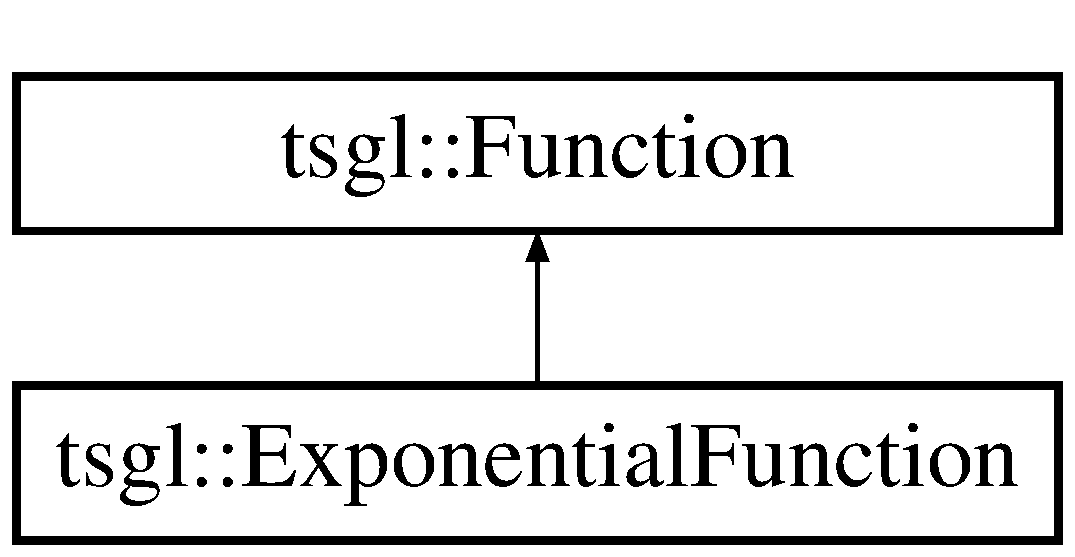
\includegraphics[height=2.000000cm]{classtsgl_1_1_exponential_function}
\end{center}
\end{figure}
\subsection*{Public Member Functions}
\begin{DoxyCompactItemize}
\item 
virtual Decimal \hyperlink{classtsgl_1_1_exponential_function_a059eae7c56a61c73b4c545b6c0e309d9}{value\+At} (Decimal x) const 
\begin{DoxyCompactList}\small\item\em Method to determine the value of \hyperlink{classtsgl_1_1_exponential_function}{Exponential\+Function}. \end{DoxyCompactList}\end{DoxyCompactItemize}


\subsection{Detailed Description}
\hyperlink{classtsgl_1_1_function}{Function} to compute e raised to the input. 

\subsection{Member Function Documentation}
\hypertarget{classtsgl_1_1_exponential_function_a059eae7c56a61c73b4c545b6c0e309d9}{}\index{tsgl\+::\+Exponential\+Function@{tsgl\+::\+Exponential\+Function}!value\+At@{value\+At}}
\index{value\+At@{value\+At}!tsgl\+::\+Exponential\+Function@{tsgl\+::\+Exponential\+Function}}
\subsubsection[{value\+At}]{\setlength{\rightskip}{0pt plus 5cm}virtual Decimal tsgl\+::\+Exponential\+Function\+::value\+At (
\begin{DoxyParamCaption}
\item[{Decimal}]{x}
\end{DoxyParamCaption}
) const\hspace{0.3cm}{\ttfamily [inline]}, {\ttfamily [virtual]}}\label{classtsgl_1_1_exponential_function_a059eae7c56a61c73b4c545b6c0e309d9}


Method to determine the value of \hyperlink{classtsgl_1_1_exponential_function}{Exponential\+Function}. 

\begin{DoxyReturn}{Returns}
{\itshape e} raised to the power of {\itshape x}. 
\end{DoxyReturn}


Implements \hyperlink{classtsgl_1_1_function_affb7b3b19a04efefa29a9870d666e912}{tsgl\+::\+Function}.



The documentation for this class was generated from the following file\+:\begin{DoxyCompactItemize}
\item 
Function.\+h\end{DoxyCompactItemize}

\hypertarget{class_f_lock}{}\section{F\+Lock Class Reference}
\label{class_f_lock}\index{F\+Lock@{F\+Lock}}


A lock giving equal priority to Readers and Writers.  




{\ttfamily \#include $<$F\+Lock.\+h$>$}

Inheritance diagram for F\+Lock\+:\begin{figure}[H]
\begin{center}
\leavevmode
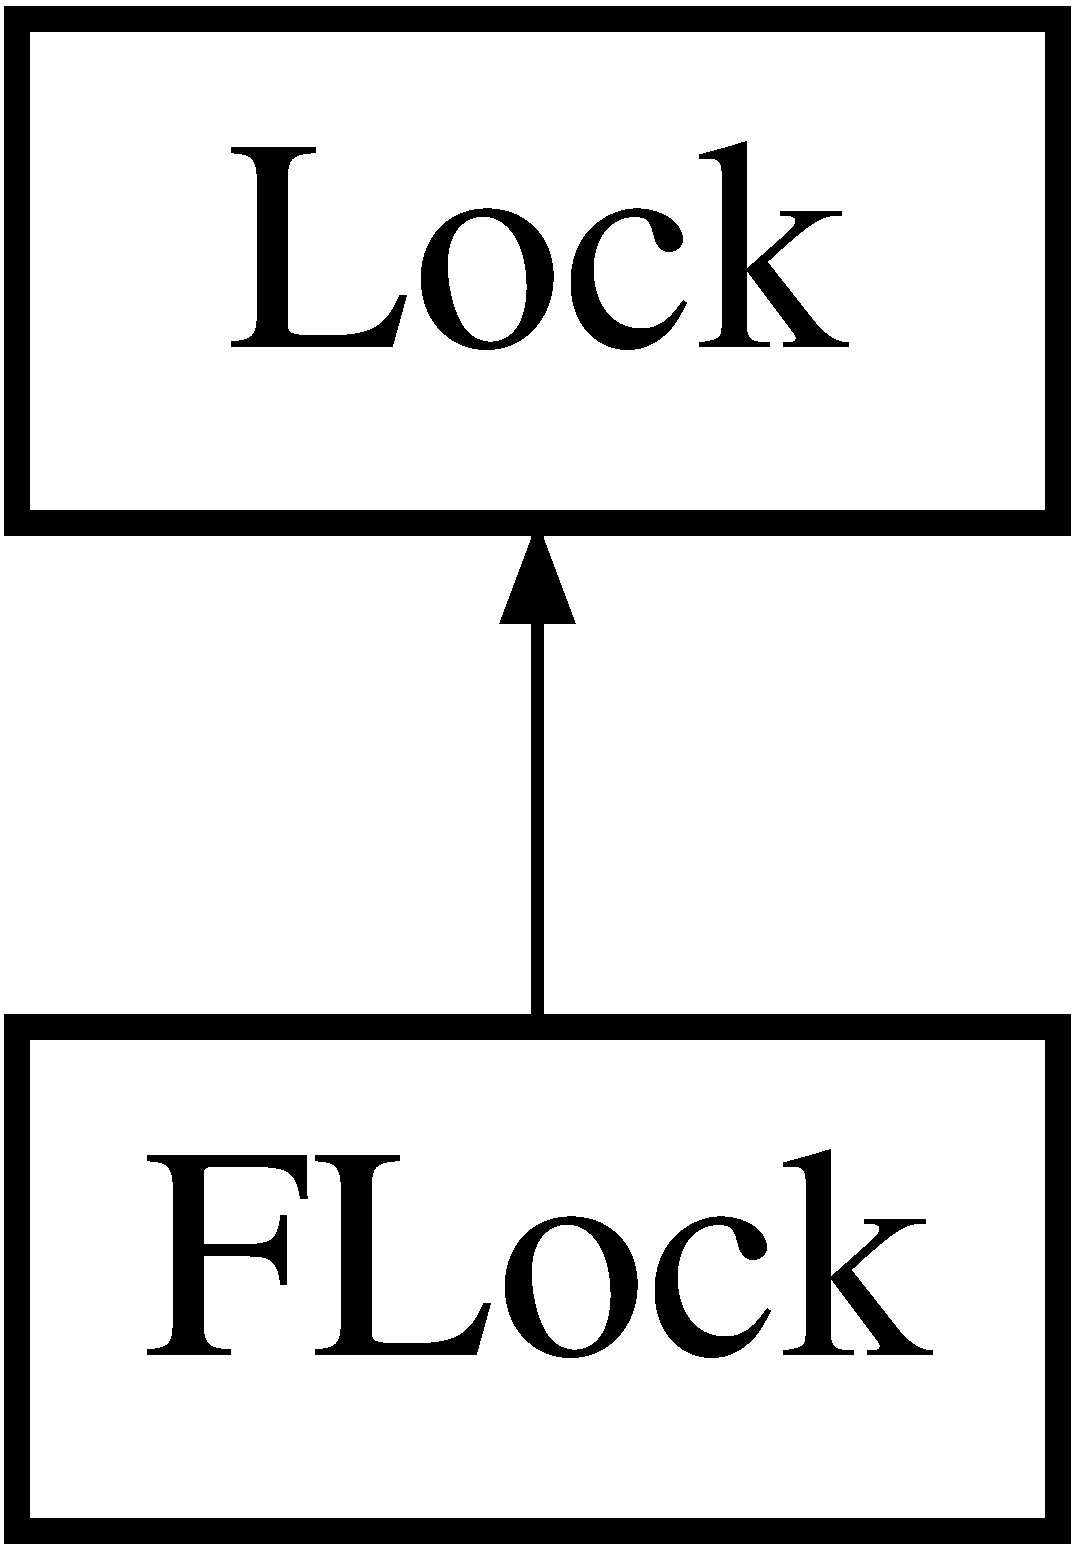
\includegraphics[height=2.000000cm]{class_f_lock}
\end{center}
\end{figure}
\subsection*{Public Member Functions}
\begin{DoxyCompactItemize}
\item 
\hyperlink{class_f_lock_a7fbb4dfce8ff879b88ff77efd4b76a96}{F\+Lock} ()
\item 
\mbox{\Hypertarget{class_f_lock_a430e0591ef1927b64124cd11085c021b}\label{class_f_lock_a430e0591ef1927b64124cd11085c021b}} 
{\bfseries F\+Lock} (\hyperlink{class_r_w_database}{R\+W\+Database}$<$ \hyperlink{classtsgl_1_1_rectangle}{tsgl\+::\+Rectangle} $\ast$$>$ $\ast$data)
\item 
void \hyperlink{class_f_lock_a8b1cde1cfe107eeb20d5f250a1c310e6}{read\+Lock} ()
\begin{DoxyCompactList}\small\item\em \hyperlink{class_f_lock_a8b1cde1cfe107eeb20d5f250a1c310e6}{read\+Lock()} implements the abstract method in \hyperlink{class_lock}{Lock} \end{DoxyCompactList}\item 
void \hyperlink{class_f_lock_ab643a836b8844cc9be52dcaf7ab18df1}{read\+Unlock} ()
\begin{DoxyCompactList}\small\item\em \hyperlink{class_f_lock_ab643a836b8844cc9be52dcaf7ab18df1}{read\+Unlock()} implements the abstract method in \hyperlink{class_lock}{Lock} \end{DoxyCompactList}\item 
void \hyperlink{class_f_lock_a4bd70bd74a3c6067f091d24a0b82edbe}{write\+Lock} ()
\begin{DoxyCompactList}\small\item\em \hyperlink{class_f_lock_a4bd70bd74a3c6067f091d24a0b82edbe}{write\+Lock()} implements the abstract method in \hyperlink{class_lock}{Lock} \end{DoxyCompactList}\item 
void \hyperlink{class_f_lock_afb22121c126a71c24e751ae7315e9a48}{write\+Unlock} ()
\begin{DoxyCompactList}\small\item\em \hyperlink{class_f_lock_afb22121c126a71c24e751ae7315e9a48}{write\+Unlock()} implements the abstract method in \hyperlink{class_lock}{Lock} \end{DoxyCompactList}\end{DoxyCompactItemize}
\subsection*{Additional Inherited Members}


\subsection{Detailed Description}
A lock giving equal priority to Readers and Writers. 

\hyperlink{_f_lock_8h_source}{F\+Lock.\+h} provides the fair monitor for the Reader-\/\+Writer visualization that gives equal preference to the Readers and Writers. This class is a subclass of \hyperlink{class_lock}{Lock} and implements its locking and unlocking virtual methods. implements the \char`\"{}commonly known solution\char`\"{} presented in\+: \href{https://arxiv.org/pdf/1309.4507.pdf}{\tt https\+://arxiv.\+org/pdf/1309.\+4507.\+pdf}

Inheritance\+: \hyperlink{class_lock}{Lock} class.

Implements the locking and unlocking methods of a monitor. 

\subsection{Constructor \& Destructor Documentation}
\mbox{\Hypertarget{class_f_lock_a7fbb4dfce8ff879b88ff77efd4b76a96}\label{class_f_lock_a7fbb4dfce8ff879b88ff77efd4b76a96}} 
\index{F\+Lock@{F\+Lock}!F\+Lock@{F\+Lock}}
\index{F\+Lock@{F\+Lock}!F\+Lock@{F\+Lock}}
\subsubsection{\texorpdfstring{F\+Lock()}{FLock()}}
{\footnotesize\ttfamily F\+Lock\+::\+F\+Lock (\begin{DoxyParamCaption}{ }\end{DoxyParamCaption})}

F\+Lock.\+cpp provides the monitor for the Reader-\/\+Writer visualization that gives a fair preference. This class is a subclass of \hyperlink{class_lock}{Lock} and implements its locking and unlocking virtual methods. 

\subsection{Member Function Documentation}
\mbox{\Hypertarget{class_f_lock_a8b1cde1cfe107eeb20d5f250a1c310e6}\label{class_f_lock_a8b1cde1cfe107eeb20d5f250a1c310e6}} 
\index{F\+Lock@{F\+Lock}!read\+Lock@{read\+Lock}}
\index{read\+Lock@{read\+Lock}!F\+Lock@{F\+Lock}}
\subsubsection{\texorpdfstring{read\+Lock()}{readLock()}}
{\footnotesize\ttfamily void F\+Lock\+::read\+Lock (\begin{DoxyParamCaption}{ }\end{DoxyParamCaption})\hspace{0.3cm}{\ttfamily [virtual]}}



\hyperlink{class_f_lock_a8b1cde1cfe107eeb20d5f250a1c310e6}{read\+Lock()} implements the abstract method in \hyperlink{class_lock}{Lock} 

Grants the calling thread access for reading 

Implements \hyperlink{class_lock}{Lock}.

\mbox{\Hypertarget{class_f_lock_ab643a836b8844cc9be52dcaf7ab18df1}\label{class_f_lock_ab643a836b8844cc9be52dcaf7ab18df1}} 
\index{F\+Lock@{F\+Lock}!read\+Unlock@{read\+Unlock}}
\index{read\+Unlock@{read\+Unlock}!F\+Lock@{F\+Lock}}
\subsubsection{\texorpdfstring{read\+Unlock()}{readUnlock()}}
{\footnotesize\ttfamily void F\+Lock\+::read\+Unlock (\begin{DoxyParamCaption}{ }\end{DoxyParamCaption})\hspace{0.3cm}{\ttfamily [virtual]}}



\hyperlink{class_f_lock_ab643a836b8844cc9be52dcaf7ab18df1}{read\+Unlock()} implements the abstract method in \hyperlink{class_lock}{Lock} 

Releases the calling thread\textquotesingle{}s read lock 

Implements \hyperlink{class_lock}{Lock}.

\mbox{\Hypertarget{class_f_lock_a4bd70bd74a3c6067f091d24a0b82edbe}\label{class_f_lock_a4bd70bd74a3c6067f091d24a0b82edbe}} 
\index{F\+Lock@{F\+Lock}!write\+Lock@{write\+Lock}}
\index{write\+Lock@{write\+Lock}!F\+Lock@{F\+Lock}}
\subsubsection{\texorpdfstring{write\+Lock()}{writeLock()}}
{\footnotesize\ttfamily void F\+Lock\+::write\+Lock (\begin{DoxyParamCaption}{ }\end{DoxyParamCaption})\hspace{0.3cm}{\ttfamily [virtual]}}



\hyperlink{class_f_lock_a4bd70bd74a3c6067f091d24a0b82edbe}{write\+Lock()} implements the abstract method in \hyperlink{class_lock}{Lock} 

Grants the calling thread acces for writing 

Implements \hyperlink{class_lock}{Lock}.

\mbox{\Hypertarget{class_f_lock_afb22121c126a71c24e751ae7315e9a48}\label{class_f_lock_afb22121c126a71c24e751ae7315e9a48}} 
\index{F\+Lock@{F\+Lock}!write\+Unlock@{write\+Unlock}}
\index{write\+Unlock@{write\+Unlock}!F\+Lock@{F\+Lock}}
\subsubsection{\texorpdfstring{write\+Unlock()}{writeUnlock()}}
{\footnotesize\ttfamily void F\+Lock\+::write\+Unlock (\begin{DoxyParamCaption}{ }\end{DoxyParamCaption})\hspace{0.3cm}{\ttfamily [virtual]}}



\hyperlink{class_f_lock_afb22121c126a71c24e751ae7315e9a48}{write\+Unlock()} implements the abstract method in \hyperlink{class_lock}{Lock} 

Releases the calling thread\textquotesingle{}s write lock 

Implements \hyperlink{class_lock}{Lock}.



The documentation for this class was generated from the following files\+:\begin{DoxyCompactItemize}
\item 
/home/sth5/test/\+T\+S\+G\+L/src/examples/\+Reader\+Writer/F\+Lock.\+h\item 
/home/sth5/test/\+T\+S\+G\+L/src/examples/\+Reader\+Writer/F\+Lock.\+cpp\end{DoxyCompactItemize}

\hypertarget{classtsgl_1_1_floor_function}{}\section{tsgl\+:\+:Floor\+Function Class Reference}
\label{classtsgl_1_1_floor_function}\index{tsgl\+::\+Floor\+Function@{tsgl\+::\+Floor\+Function}}


\hyperlink{classtsgl_1_1_function}{Function} to compute the mathematical floor of the input.  




{\ttfamily \#include $<$Function.\+h$>$}

Inheritance diagram for tsgl\+:\+:Floor\+Function\+:\begin{figure}[H]
\begin{center}
\leavevmode
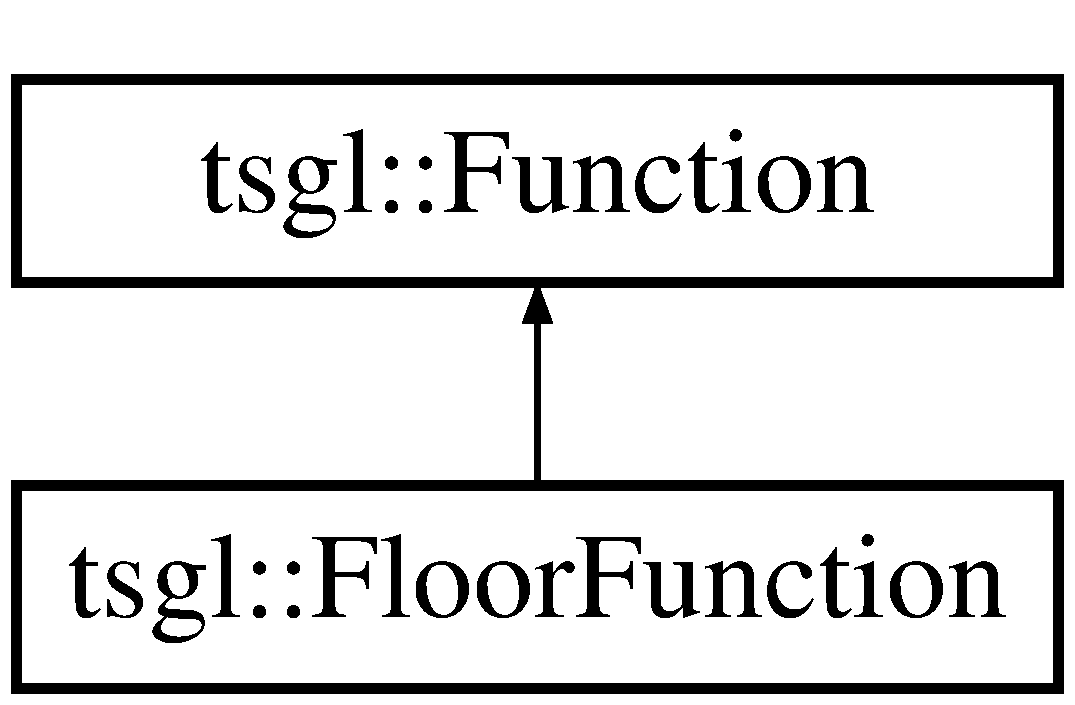
\includegraphics[height=2.000000cm]{classtsgl_1_1_floor_function}
\end{center}
\end{figure}
\subsection*{Public Member Functions}
\begin{DoxyCompactItemize}
\item 
virtual Decimal \hyperlink{classtsgl_1_1_floor_function_a28fae5b310ae965348fb2eaec50fd5c8}{value\+At} (Decimal x) const
\begin{DoxyCompactList}\small\item\em Method to determine the value of \hyperlink{classtsgl_1_1_floor_function}{Floor\+Function}. \end{DoxyCompactList}\end{DoxyCompactItemize}


\subsection{Detailed Description}
\hyperlink{classtsgl_1_1_function}{Function} to compute the mathematical floor of the input. 

\subsection{Member Function Documentation}
\mbox{\Hypertarget{classtsgl_1_1_floor_function_a28fae5b310ae965348fb2eaec50fd5c8}\label{classtsgl_1_1_floor_function_a28fae5b310ae965348fb2eaec50fd5c8}} 
\index{tsgl\+::\+Floor\+Function@{tsgl\+::\+Floor\+Function}!value\+At@{value\+At}}
\index{value\+At@{value\+At}!tsgl\+::\+Floor\+Function@{tsgl\+::\+Floor\+Function}}
\subsubsection{\texorpdfstring{value\+At()}{valueAt()}}
{\footnotesize\ttfamily virtual Decimal tsgl\+::\+Floor\+Function\+::value\+At (\begin{DoxyParamCaption}\item[{Decimal}]{x }\end{DoxyParamCaption}) const\hspace{0.3cm}{\ttfamily [inline]}, {\ttfamily [virtual]}}



Method to determine the value of \hyperlink{classtsgl_1_1_floor_function}{Floor\+Function}. 

\begin{DoxyReturn}{Returns}
The largest integer less than or equal to {\itshape x}. 
\end{DoxyReturn}


Implements \hyperlink{classtsgl_1_1_function_affb7b3b19a04efefa29a9870d666e912}{tsgl\+::\+Function}.



The documentation for this class was generated from the following file\+:\begin{DoxyCompactItemize}
\item 
Function.\+h\end{DoxyCompactItemize}

\hypertarget{struct_fork}{}\section{Fork Struct Reference}
\label{struct_fork}\index{Fork@{Fork}}


Struct for the forks in the Dining Philosophers\textquotesingle{} problem.  




{\ttfamily \#include $<$Fork.\+h$>$}

\subsection*{Public Member Functions}
\begin{DoxyCompactItemize}
\item 
\mbox{\Hypertarget{struct_fork_a17aae2a4e6464c2ec8ac439443b7433e}\label{struct_fork_a17aae2a4e6464c2ec8ac439443b7433e}} 
void {\bfseries set\+Canvas} (\hyperlink{classtsgl_1_1_canvas}{Canvas} $\ast$can)
\item 
\mbox{\Hypertarget{struct_fork_a037d640832899cd5cad90b2c2ea4f4ec}\label{struct_fork_a037d640832899cd5cad90b2c2ea4f4ec}} 
void {\bfseries draw} (float x, float y, double angle, \hyperlink{structtsgl_1_1_color_float}{Color\+Float} c)
\end{DoxyCompactItemize}
\subsection*{Public Attributes}
\begin{DoxyCompactItemize}
\item 
\mbox{\Hypertarget{struct_fork_a28995f27196a2b80cf48024fd728d7df}\label{struct_fork_a28995f27196a2b80cf48024fd728d7df}} 
int {\bfseries user}
\item 
\mbox{\Hypertarget{struct_fork_a72d6934869569aea1806a74e544b05f3}\label{struct_fork_a72d6934869569aea1806a74e544b05f3}} 
int {\bfseries id}
\item 
\mbox{\Hypertarget{struct_fork_aa1cd6cedb40e543d1ae4e7c8d9db24d7}\label{struct_fork_aa1cd6cedb40e543d1ae4e7c8d9db24d7}} 
\hyperlink{classtsgl_1_1_concave_polygon}{Concave\+Polygon} $\ast$ {\bfseries my\+Shape}
\end{DoxyCompactItemize}


\subsection{Detailed Description}
Struct for the forks in the Dining Philosophers\textquotesingle{} problem. 

The documentation for this struct was generated from the following file\+:\begin{DoxyCompactItemize}
\item 
/home/sth5/test/\+T\+S\+G\+L/src/examples/\+Dining\+Philosophers/Fork.\+h\end{DoxyCompactItemize}

\hypertarget{struct_fork3_d}{}\section{Fork3D Struct Reference}
\label{struct_fork3_d}\index{Fork3D@{Fork3D}}


Struct for the forks in the 3D visualization of the Dining Philosophers\textquotesingle{} problem.  




{\ttfamily \#include $<$Fork3\+D.\+h$>$}

\subsection*{Public Member Functions}
\begin{DoxyCompactItemize}
\item 
\mbox{\Hypertarget{struct_fork3_d_a2f341294fbd07eba8f81a4e5bfeb4e95}\label{struct_fork3_d_a2f341294fbd07eba8f81a4e5bfeb4e95}} 
void {\bfseries set\+Canvas} (\hyperlink{classtsgl_1_1_canvas}{Canvas} $\ast$can)
\item 
\mbox{\Hypertarget{struct_fork3_d_aa745d8afac91a5a4ae335d8f1262ae6f}\label{struct_fork3_d_aa745d8afac91a5a4ae335d8f1262ae6f}} 
void {\bfseries draw} (float x, float y, double angle, \hyperlink{structtsgl_1_1_color_float}{Color\+Float} c)
\end{DoxyCompactItemize}
\subsection*{Public Attributes}
\begin{DoxyCompactItemize}
\item 
\mbox{\Hypertarget{struct_fork3_d_a2ac3101fcd371e6357fc25dcfb9ecbe3}\label{struct_fork3_d_a2ac3101fcd371e6357fc25dcfb9ecbe3}} 
int {\bfseries user}
\item 
\mbox{\Hypertarget{struct_fork3_d_abdf1bb4422ffdf7922024525aab94d67}\label{struct_fork3_d_abdf1bb4422ffdf7922024525aab94d67}} 
int {\bfseries id}
\item 
\mbox{\Hypertarget{struct_fork3_d_a84c898115b60f9673152c88998463f60}\label{struct_fork3_d_a84c898115b60f9673152c88998463f60}} 
\hyperlink{classtsgl_1_1_concave_polygon}{Concave\+Polygon} $\ast$ {\bfseries my\+Shape}
\end{DoxyCompactItemize}


\subsection{Detailed Description}
Struct for the forks in the 3D visualization of the Dining Philosophers\textquotesingle{} problem. 

The documentation for this struct was generated from the following file\+:\begin{DoxyCompactItemize}
\item 
/home/sth5/test/\+T\+S\+G\+L/src/examples/\+Dining\+Philosophers3\+D/Fork3\+D.\+h\end{DoxyCompactItemize}

\hypertarget{classtsgl_1_1_function}{}\section{tsgl\+:\+:Function Class Reference}
\label{classtsgl_1_1_function}\index{tsgl\+::\+Function@{tsgl\+::\+Function}}


A base class for creating mathematical functions plottable by a \hyperlink{classtsgl_1_1_cartesian_canvas}{Cartesian\+Canvas}.  




{\ttfamily \#include $<$Function.\+h$>$}

Inheritance diagram for tsgl\+:\+:Function\+:\begin{figure}[H]
\begin{center}
\leavevmode
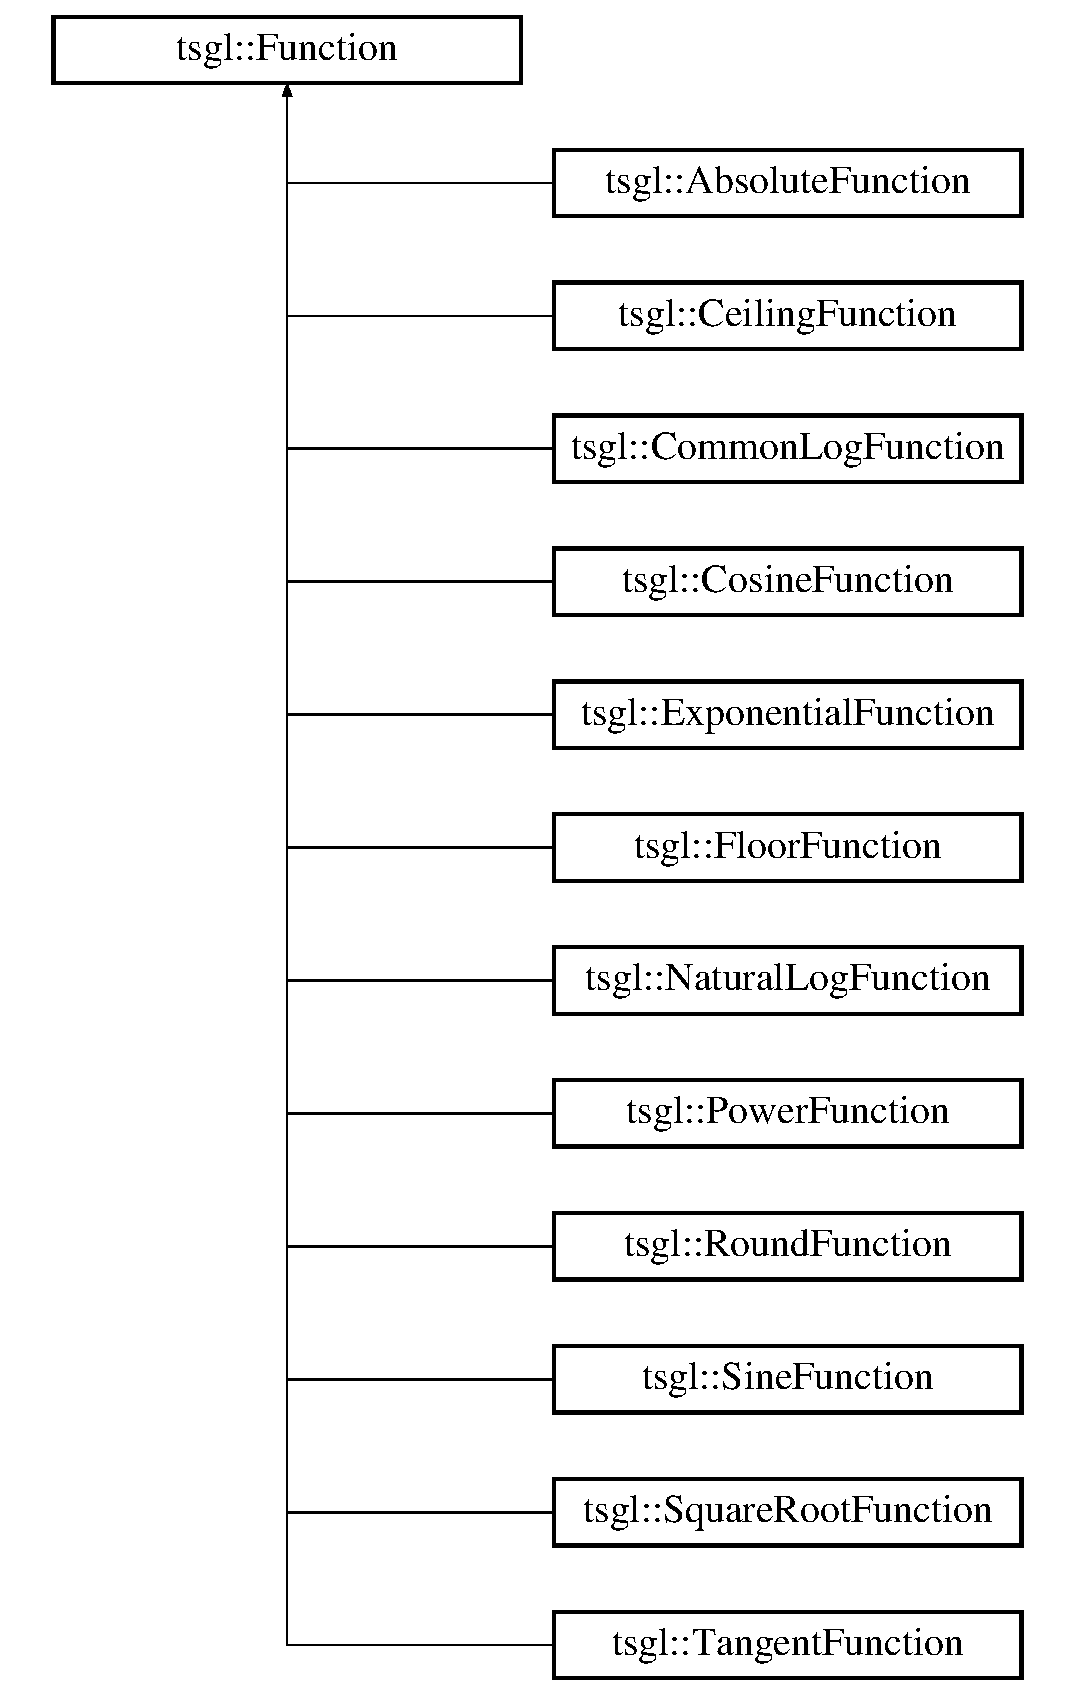
\includegraphics[height=12.000000cm]{classtsgl_1_1_function}
\end{center}
\end{figure}
\subsection*{Public Member Functions}
\begin{DoxyCompactItemize}
\item 
\hyperlink{classtsgl_1_1_function_aaf959c9d39bb45c2aded83fd754c288d}{Function} ()
\begin{DoxyCompactList}\small\item\em Constructs a new \hyperlink{classtsgl_1_1_function}{Function}. \end{DoxyCompactList}\item 
virtual \hyperlink{classtsgl_1_1_function_a3b8cbd26a32c6ae75b12e7397bb42c41}{$\sim$\+Function} ()
\begin{DoxyCompactList}\small\item\em Destructor for the \hyperlink{classtsgl_1_1_function}{Function} class. \end{DoxyCompactList}\item 
virtual Decimal \hyperlink{classtsgl_1_1_function_affb7b3b19a04efefa29a9870d666e912}{value\+At} (Decimal x) const =0
\begin{DoxyCompactList}\small\item\em Method to determine the value of a \hyperlink{classtsgl_1_1_function}{Function} subclass. \end{DoxyCompactList}\end{DoxyCompactItemize}


\subsection{Detailed Description}
A base class for creating mathematical functions plottable by a \hyperlink{classtsgl_1_1_cartesian_canvas}{Cartesian\+Canvas}. 

\hyperlink{classtsgl_1_1_function}{Function} provides a base class for the creation of mathematical functions. By extending this class and overriding the \hyperlink{classtsgl_1_1_function_affb7b3b19a04efefa29a9870d666e912}{value\+At()} method, users can easily plot the values of their function on a \hyperlink{classtsgl_1_1_cartesian_canvas}{Cartesian\+Canvas}.

A number of pre-\/built \hyperlink{classtsgl_1_1_function}{Function} subclasses are included in the header file for reference. 

\subsection{Constructor \& Destructor Documentation}
\mbox{\Hypertarget{classtsgl_1_1_function_aaf959c9d39bb45c2aded83fd754c288d}\label{classtsgl_1_1_function_aaf959c9d39bb45c2aded83fd754c288d}} 
\index{tsgl\+::\+Function@{tsgl\+::\+Function}!Function@{Function}}
\index{Function@{Function}!tsgl\+::\+Function@{tsgl\+::\+Function}}
\subsubsection{\texorpdfstring{Function()}{Function()}}
{\footnotesize\ttfamily tsgl\+::\+Function\+::\+Function (\begin{DoxyParamCaption}{ }\end{DoxyParamCaption})\hspace{0.3cm}{\ttfamily [inline]}}



Constructs a new \hyperlink{classtsgl_1_1_function}{Function}. 

This is the default constructor for the \hyperlink{classtsgl_1_1_function}{Function} class. \begin{DoxyNote}{Note}
The default constructor for the parent \hyperlink{classtsgl_1_1_function}{Function} class does absolutely nothing. Any construction should be defined in the subclass. 
\end{DoxyNote}
\mbox{\Hypertarget{classtsgl_1_1_function_a3b8cbd26a32c6ae75b12e7397bb42c41}\label{classtsgl_1_1_function_a3b8cbd26a32c6ae75b12e7397bb42c41}} 
\index{tsgl\+::\+Function@{tsgl\+::\+Function}!````~Function@{$\sim$\+Function}}
\index{````~Function@{$\sim$\+Function}!tsgl\+::\+Function@{tsgl\+::\+Function}}
\subsubsection{\texorpdfstring{$\sim$\+Function()}{~Function()}}
{\footnotesize\ttfamily virtual tsgl\+::\+Function\+::$\sim$\+Function (\begin{DoxyParamCaption}{ }\end{DoxyParamCaption})\hspace{0.3cm}{\ttfamily [inline]}, {\ttfamily [virtual]}}



Destructor for the \hyperlink{classtsgl_1_1_function}{Function} class. 

\begin{DoxyNote}{Note}
The default destructor for the parent \hyperlink{classtsgl_1_1_function}{Function} class does absolutely nothing. Any destruction should be defined in the subclass. 
\end{DoxyNote}


\subsection{Member Function Documentation}
\mbox{\Hypertarget{classtsgl_1_1_function_affb7b3b19a04efefa29a9870d666e912}\label{classtsgl_1_1_function_affb7b3b19a04efefa29a9870d666e912}} 
\index{tsgl\+::\+Function@{tsgl\+::\+Function}!value\+At@{value\+At}}
\index{value\+At@{value\+At}!tsgl\+::\+Function@{tsgl\+::\+Function}}
\subsubsection{\texorpdfstring{value\+At()}{valueAt()}}
{\footnotesize\ttfamily virtual Decimal tsgl\+::\+Function\+::value\+At (\begin{DoxyParamCaption}\item[{Decimal}]{x }\end{DoxyParamCaption}) const\hspace{0.3cm}{\ttfamily [pure virtual]}}



Method to determine the value of a \hyperlink{classtsgl_1_1_function}{Function} subclass. 

This method should be overridden with the actual function you want to compute. 
\begin{DoxyParams}{Parameters}
{\em x} & The input to the function. Assuming your function is F, x will be used to compute F(x). \\
\hline
\end{DoxyParams}
\begin{DoxyReturn}{Returns}
The Decimal value of F(x). 
\end{DoxyReturn}
\begin{DoxyNote}{Note}
This method is abstract and {\bfseries must} be overridden. 
\end{DoxyNote}


Implemented in \hyperlink{classtsgl_1_1_round_function_ad01ca0b18d7b5f3f8c5a49181b1dc922}{tsgl\+::\+Round\+Function}, \hyperlink{classtsgl_1_1_floor_function_a28fae5b310ae965348fb2eaec50fd5c8}{tsgl\+::\+Floor\+Function}, \hyperlink{classtsgl_1_1_ceiling_function_a01487798ff6e2adc9481177e96e4e89c}{tsgl\+::\+Ceiling\+Function}, \hyperlink{classtsgl_1_1_common_log_function_a18f2c4f8779309e0d1c936a0589b1f3a}{tsgl\+::\+Common\+Log\+Function}, \hyperlink{classtsgl_1_1_natural_log_function_a27894f0360a0f89cf01126781a36e500}{tsgl\+::\+Natural\+Log\+Function}, \hyperlink{classtsgl_1_1_exponential_function_a65c7a08da7e5e0bdbf5dbcb13f046eb5}{tsgl\+::\+Exponential\+Function}, \hyperlink{classtsgl_1_1_absolute_function_a57c7114b54ebfc4a35da1b5e9374e495}{tsgl\+::\+Absolute\+Function}, \hyperlink{classtsgl_1_1_tangent_function_af0ca18ffd1bccefb8ede5c1121e3813c}{tsgl\+::\+Tangent\+Function}, \hyperlink{classtsgl_1_1_cosine_function_a2d7841c4f9f77bdd8f5bbc51cbd80bcd}{tsgl\+::\+Cosine\+Function}, \hyperlink{classtsgl_1_1_sine_function_a4a34d3310ea217255124d5e35805be3a}{tsgl\+::\+Sine\+Function}, \hyperlink{classtsgl_1_1_square_root_function_ad77fa33b36dcf3bcb7d7957e489bf33f}{tsgl\+::\+Square\+Root\+Function}, and \hyperlink{classtsgl_1_1_power_function_a1dfcce604dd60b033969807f6312b074}{tsgl\+::\+Power\+Function}.



Referenced by $\sim$\+Function().



The documentation for this class was generated from the following file\+:\begin{DoxyCompactItemize}
\item 
Function.\+h\end{DoxyCompactItemize}

\hypertarget{class_gradient_mandelbrot}{}\section{Gradient\+Mandelbrot Class Reference}
\label{class_gradient_mandelbrot}\index{Gradient\+Mandelbrot@{Gradient\+Mandelbrot}}


Draws a \hyperlink{class_gradient_mandelbrot}{Gradient\+Mandelbrot} set on a Cartesian\+Canvas.  




{\ttfamily \#include $<$Gradient\+Mandelbrot.\+h$>$}

Inheritance diagram for Gradient\+Mandelbrot\+:\begin{figure}[H]
\begin{center}
\leavevmode
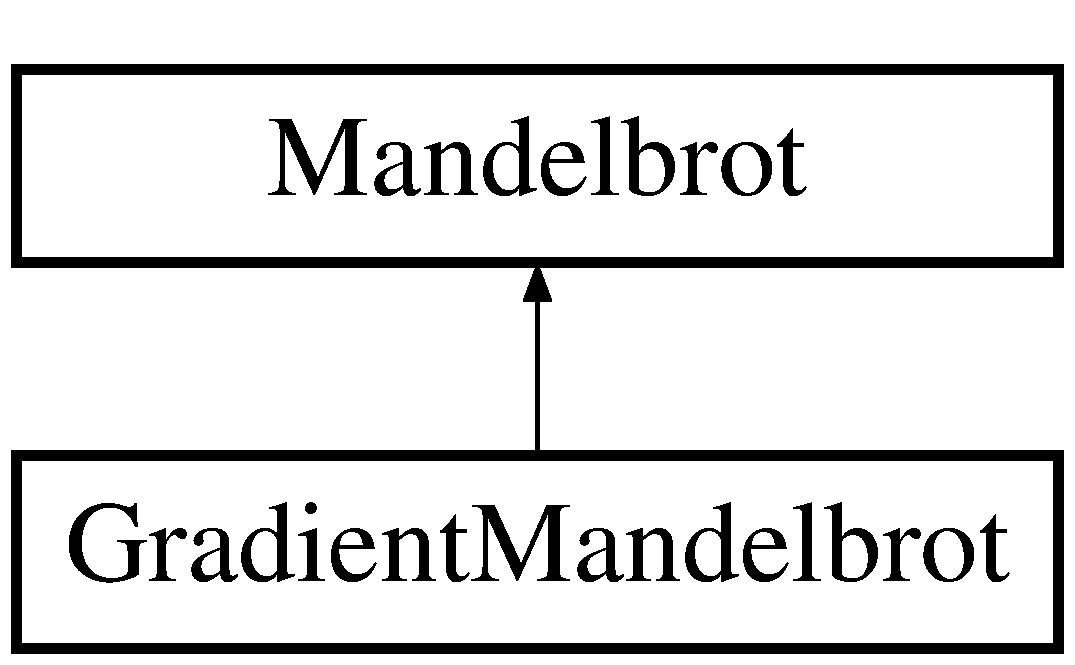
\includegraphics[height=2.000000cm]{class_gradient_mandelbrot}
\end{center}
\end{figure}
\subsection*{Public Member Functions}
\begin{DoxyCompactItemize}
\item 
\hyperlink{class_gradient_mandelbrot_a4284747d6cef5b030fc82ffea41c850d}{Gradient\+Mandelbrot} (unsigned threads, unsigned depth)
\begin{DoxyCompactList}\small\item\em Explicitly constructs a \hyperlink{class_gradient_mandelbrot}{Gradient\+Mandelbrot} set. \end{DoxyCompactList}\item 
void \hyperlink{class_gradient_mandelbrot_a1d4aa3e44d7d1c2241545b60c79985df}{draw} (\hyperlink{classtsgl_1_1_cartesian_canvas}{Cart} \&can)
\begin{DoxyCompactList}\small\item\em Draw the \hyperlink{class_gradient_mandelbrot}{Gradient\+Mandelbrot} set. \end{DoxyCompactList}\end{DoxyCompactItemize}
\subsection*{Additional Inherited Members}


\subsection{Detailed Description}
Draws a \hyperlink{class_gradient_mandelbrot}{Gradient\+Mandelbrot} set on a Cartesian\+Canvas. 

Similar to a normal \hyperlink{class_mandelbrot}{Mandelbrot} set but with a smoother shading.

Extends the \hyperlink{class_mandelbrot}{Mandelbrot} class and overrides its \hyperlink{class_gradient_mandelbrot_a1d4aa3e44d7d1c2241545b60c79985df}{draw()} function and set\+Redraw() function.

Can zoom in and out of the \hyperlink{class_mandelbrot}{Mandelbrot} set by scrolling up and down on the mouse wheel (respectively). \begin{DoxySeeAlso}{See also}
\hyperlink{class_mandelbrot}{Mandelbrot} class 
\end{DoxySeeAlso}


\subsection{Constructor \& Destructor Documentation}
\mbox{\Hypertarget{class_gradient_mandelbrot_a4284747d6cef5b030fc82ffea41c850d}\label{class_gradient_mandelbrot_a4284747d6cef5b030fc82ffea41c850d}} 
\index{Gradient\+Mandelbrot@{Gradient\+Mandelbrot}!Gradient\+Mandelbrot@{Gradient\+Mandelbrot}}
\index{Gradient\+Mandelbrot@{Gradient\+Mandelbrot}!Gradient\+Mandelbrot@{Gradient\+Mandelbrot}}
\subsubsection{\texorpdfstring{Gradient\+Mandelbrot()}{GradientMandelbrot()}}
{\footnotesize\ttfamily Gradient\+Mandelbrot\+::\+Gradient\+Mandelbrot (\begin{DoxyParamCaption}\item[{unsigned}]{threads,  }\item[{unsigned}]{depth }\end{DoxyParamCaption})}



Explicitly constructs a \hyperlink{class_gradient_mandelbrot}{Gradient\+Mandelbrot} set. 

Explicit constructor for the Gradien\+Mandelbrot class. 
\begin{DoxyParams}{Parameters}
{\em threads} & The number of threads to use in the drawing of the \hyperlink{class_gradient_mandelbrot}{Gradient\+Mandelbrot} object. \\
\hline
{\em depth} & The number of iterations to go to in order to draw the \hyperlink{class_gradient_mandelbrot}{Gradient\+Mandelbrot} object. \\
\hline
\end{DoxyParams}
\begin{DoxyReturn}{Returns}
The \hyperlink{class_gradient_mandelbrot}{Gradient\+Mandelbrot} object ready to be drawn onto the Cartesian\+Canvas. 
\end{DoxyReturn}


\subsection{Member Function Documentation}
\mbox{\Hypertarget{class_gradient_mandelbrot_a1d4aa3e44d7d1c2241545b60c79985df}\label{class_gradient_mandelbrot_a1d4aa3e44d7d1c2241545b60c79985df}} 
\index{Gradient\+Mandelbrot@{Gradient\+Mandelbrot}!draw@{draw}}
\index{draw@{draw}!Gradient\+Mandelbrot@{Gradient\+Mandelbrot}}
\subsubsection{\texorpdfstring{draw()}{draw()}}
{\footnotesize\ttfamily void Gradient\+Mandelbrot\+::draw (\begin{DoxyParamCaption}\item[{\hyperlink{classtsgl_1_1_cartesian_canvas}{Cart} \&}]{can }\end{DoxyParamCaption})\hspace{0.3cm}{\ttfamily [virtual]}}



Draw the \hyperlink{class_gradient_mandelbrot}{Gradient\+Mandelbrot} set. 

Actually draws the \hyperlink{class_gradient_mandelbrot}{Gradient\+Mandelbrot} set onto the Cartesian\+Canvas. 
\begin{DoxyParams}{Parameters}
{\em can} & Reference to the Cartesian\+Canvas to draw to. \\
\hline
\end{DoxyParams}
\begin{DoxyNote}{Note}
This method overrides the \hyperlink{class_mandelbrot}{Mandelbrot} class\textquotesingle{} \hyperlink{class_gradient_mandelbrot_a1d4aa3e44d7d1c2241545b60c79985df}{draw()} method. 

Cart is a typedef for a Cartesian\+Canvas object. 
\end{DoxyNote}


Reimplemented from \hyperlink{class_mandelbrot_ab7918e4de8f00f73290f110ca7a6cffd}{Mandelbrot}.



The documentation for this class was generated from the following files\+:\begin{DoxyCompactItemize}
\item 
/home/sth5/test/\+T\+S\+G\+L/src/examples/\+Mandelbrot/Gradient\+Mandelbrot.\+h\item 
/home/sth5/test/\+T\+S\+G\+L/src/examples/\+Mandelbrot/Gradient\+Mandelbrot.\+cpp\end{DoxyCompactItemize}

\hypertarget{classtsgl_1_1_image}{}\section{tsgl\+:\+:Image Class Reference}
\label{classtsgl_1_1_image}\index{tsgl\+::\+Image@{tsgl\+::\+Image}}


Draw an image to the \hyperlink{classtsgl_1_1_canvas}{Canvas}.  




{\ttfamily \#include $<$Image.\+h$>$}

Inheritance diagram for tsgl\+:\+:Image\+:\begin{figure}[H]
\begin{center}
\leavevmode
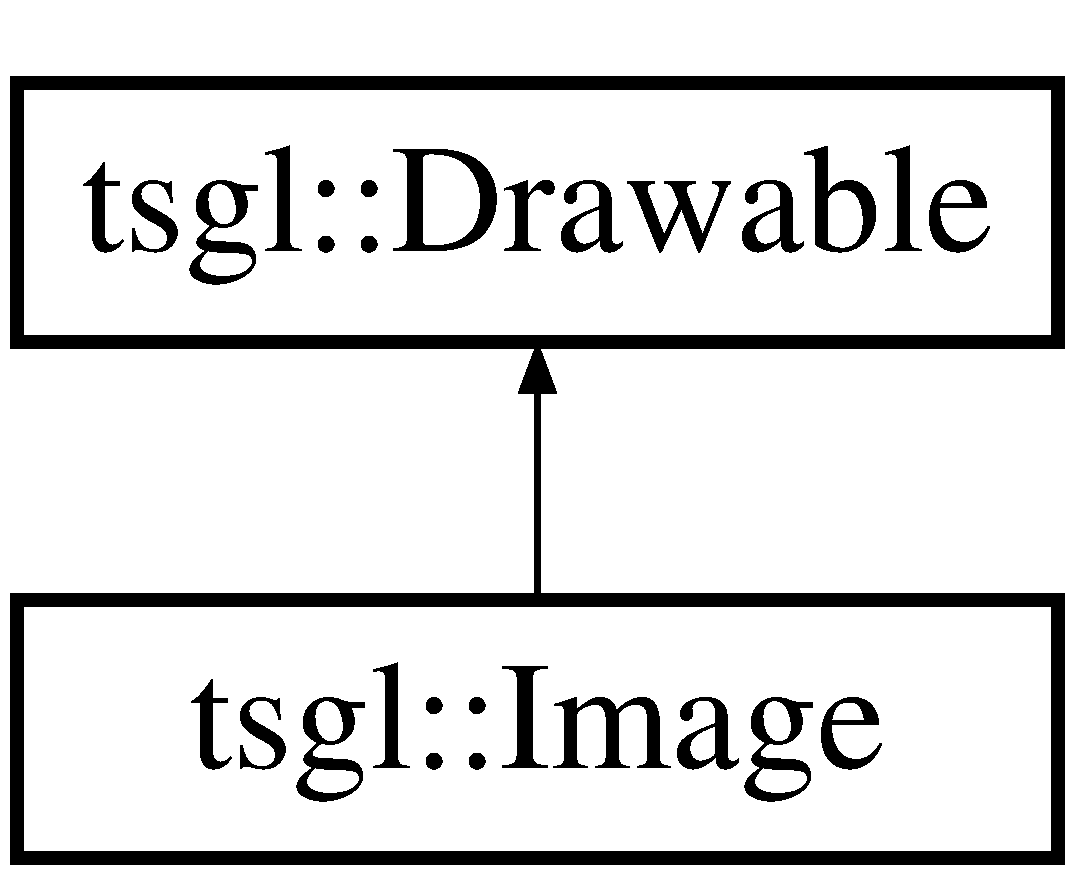
\includegraphics[height=2.000000cm]{classtsgl_1_1_image}
\end{center}
\end{figure}
\subsection*{Public Member Functions}
\begin{DoxyCompactItemize}
\item 
\hyperlink{classtsgl_1_1_image_a497894a4dbfa46d1e3aefd7dbe086cc3}{Image} (std\+::string filename, \hyperlink{classtsgl_1_1_texture_handler}{Texture\+Handler} \&loader, int x, int y, int width, int height, float alpha)
\begin{DoxyCompactList}\small\item\em Explicitly constructs a new \hyperlink{classtsgl_1_1_image}{Image}. \end{DoxyCompactList}\item 
void \hyperlink{classtsgl_1_1_image_a85732de312b98dd5ce5a9cc319bbf8c5}{draw} ()
\begin{DoxyCompactList}\small\item\em Draw the \hyperlink{classtsgl_1_1_image}{Image}. \end{DoxyCompactList}\item 
int \hyperlink{classtsgl_1_1_image_afa939262dcf32c9a504efe30a8de5c58}{get\+Height} ()
\begin{DoxyCompactList}\small\item\em Accessor for the image\textquotesingle{}s height. \end{DoxyCompactList}\item 
int \hyperlink{classtsgl_1_1_image_af01d5f815b91f20fd441f9bcec671d79}{get\+Width} ()
\begin{DoxyCompactList}\small\item\em Accessor for the image\textquotesingle{}s width. \end{DoxyCompactList}\end{DoxyCompactItemize}
\subsection*{Additional Inherited Members}


\subsection{Detailed Description}
Draw an image to the \hyperlink{classtsgl_1_1_canvas}{Canvas}. 

\hyperlink{classtsgl_1_1_image}{Image} is a class which provides a simple interface for loading and drawing images. The \hyperlink{classtsgl_1_1_image}{Image} class currently supports files in the .png, .bmp, and .jpg formats. \begin{DoxyNote}{Note}
For the time being, there is no way to measure the size of an image once it\textquotesingle{}s loaded. Therefore, the width and height must be specified manually, and stretching may occur if the input dimensions don\textquotesingle{}t match the images actual dimensions. 

Additionally, an Image\+Loader must be passed as an argument. This Image\+Loader is automatically constructed with the \hyperlink{classtsgl_1_1_canvas}{Canvas} as the private {\itshape loader} variable. At the moment, there is no way to extend \hyperlink{classtsgl_1_1_canvas_ae94a586629d20b7fabcb402d1c654628}{Canvas\+::draw\+Image()} function due to this privatization. 
\end{DoxyNote}
\begin{DoxyWarning}{Warning}
Aside from an error message output to stderr, \hyperlink{classtsgl_1_1_image}{Image} gives no indication if an image failed to load. 
\end{DoxyWarning}


\subsection{Constructor \& Destructor Documentation}
\hypertarget{classtsgl_1_1_image_a497894a4dbfa46d1e3aefd7dbe086cc3}{}\index{tsgl\+::\+Image@{tsgl\+::\+Image}!Image@{Image}}
\index{Image@{Image}!tsgl\+::\+Image@{tsgl\+::\+Image}}
\subsubsection[{Image}]{\setlength{\rightskip}{0pt plus 5cm}tsgl\+::\+Image\+::\+Image (
\begin{DoxyParamCaption}
\item[{std\+::string}]{filename, }
\item[{{\bf Texture\+Handler} \&}]{loader, }
\item[{int}]{x, }
\item[{int}]{y, }
\item[{int}]{width, }
\item[{int}]{height, }
\item[{float}]{alpha}
\end{DoxyParamCaption}
)}\label{classtsgl_1_1_image_a497894a4dbfa46d1e3aefd7dbe086cc3}


Explicitly constructs a new \hyperlink{classtsgl_1_1_image}{Image}. 

This is the explicit constructor for the \hyperlink{classtsgl_1_1_image}{Image} class. 
\begin{DoxyParams}{Parameters}
{\em filename} & The filename of the image to load. \\
\hline
{\em loader} & A reference pointer to the \hyperlink{classtsgl_1_1_texture_handler}{Texture\+Handler} with which to load the image. \\
\hline
{\em x} & The x coordinate of the left of the \hyperlink{classtsgl_1_1_image}{Image}. \\
\hline
{\em y} & The y coordinate of the top of the \hyperlink{classtsgl_1_1_image}{Image}. \\
\hline
{\em width} & The width of the \hyperlink{classtsgl_1_1_image}{Image}. \\
\hline
{\em height} & The height of the \hyperlink{classtsgl_1_1_image}{Image}. \\
\hline
{\em alhpa} & The alpha of the \hyperlink{classtsgl_1_1_image}{Image}. \\
\hline
\end{DoxyParams}
\begin{DoxyReturn}{Returns}
A new \hyperlink{classtsgl_1_1_image}{Image} is drawn with the specified coordinates, dimensions, and transparency. 
\end{DoxyReturn}
\begin{DoxyNote}{Note}
{\bfseries I\+M\+P\+O\+R\+T\+A\+N\+T}\+: In \hyperlink{classtsgl_1_1_cartesian_canvas}{Cartesian\+Canvas}, {\itshape y} specifies the bottom, not the top, of the image. 
\end{DoxyNote}


\subsection{Member Function Documentation}
\hypertarget{classtsgl_1_1_image_a85732de312b98dd5ce5a9cc319bbf8c5}{}\index{tsgl\+::\+Image@{tsgl\+::\+Image}!draw@{draw}}
\index{draw@{draw}!tsgl\+::\+Image@{tsgl\+::\+Image}}
\subsubsection[{draw}]{\setlength{\rightskip}{0pt plus 5cm}void tsgl\+::\+Image\+::draw (
\begin{DoxyParamCaption}
{}
\end{DoxyParamCaption}
)\hspace{0.3cm}{\ttfamily [virtual]}}\label{classtsgl_1_1_image_a85732de312b98dd5ce5a9cc319bbf8c5}


Draw the \hyperlink{classtsgl_1_1_image}{Image}. 

This function actually draws the \hyperlink{classtsgl_1_1_image}{Image} to the \hyperlink{classtsgl_1_1_canvas}{Canvas}. 

Implements \hyperlink{classtsgl_1_1_shape_af78b1627b97d621824ce86db214e2402}{tsgl\+::\+Shape}.

\hypertarget{classtsgl_1_1_image_afa939262dcf32c9a504efe30a8de5c58}{}\index{tsgl\+::\+Image@{tsgl\+::\+Image}!get\+Height@{get\+Height}}
\index{get\+Height@{get\+Height}!tsgl\+::\+Image@{tsgl\+::\+Image}}
\subsubsection[{get\+Height}]{\setlength{\rightskip}{0pt plus 5cm}int tsgl\+::\+Image\+::get\+Height (
\begin{DoxyParamCaption}
{}
\end{DoxyParamCaption}
)\hspace{0.3cm}{\ttfamily [inline]}}\label{classtsgl_1_1_image_afa939262dcf32c9a504efe30a8de5c58}


Accessor for the image\textquotesingle{}s height. 

\begin{DoxyReturn}{Returns}
The height of the \hyperlink{classtsgl_1_1_image}{Image}. 
\end{DoxyReturn}
\hypertarget{classtsgl_1_1_image_af01d5f815b91f20fd441f9bcec671d79}{}\index{tsgl\+::\+Image@{tsgl\+::\+Image}!get\+Width@{get\+Width}}
\index{get\+Width@{get\+Width}!tsgl\+::\+Image@{tsgl\+::\+Image}}
\subsubsection[{get\+Width}]{\setlength{\rightskip}{0pt plus 5cm}int tsgl\+::\+Image\+::get\+Width (
\begin{DoxyParamCaption}
{}
\end{DoxyParamCaption}
)\hspace{0.3cm}{\ttfamily [inline]}}\label{classtsgl_1_1_image_af01d5f815b91f20fd441f9bcec671d79}


Accessor for the image\textquotesingle{}s width. 

\begin{DoxyReturn}{Returns}
The width of the \hyperlink{classtsgl_1_1_image}{Image}. 
\end{DoxyReturn}


The documentation for this class was generated from the following files\+:\begin{DoxyCompactItemize}
\item 
Image.\+h\item 
Image.\+cpp\end{DoxyCompactItemize}

\hypertarget{classtsgl_1_1_integral_viewer}{}\section{tsgl\+:\+:Integral\+Viewer Class Reference}
\label{classtsgl_1_1_integral_viewer}\index{tsgl\+::\+Integral\+Viewer@{tsgl\+::\+Integral\+Viewer}}


Provides a a tool for computing and visualizing integrals of functions.  




{\ttfamily \#include $<$Integral\+Viewer.\+h$>$}

\subsection*{Public Member Functions}
\begin{DoxyCompactItemize}
\item 
\hyperlink{classtsgl_1_1_integral_viewer_a1fe15a118865fcaf3067dc73cf3f912c}{Integral\+Viewer} (function\+Pointer f, int width, int height, Decimal startX, Decimal stopX, Decimal startY=0, Decimal stopY=1, std\+::string fname=\char`\"{}function\char`\"{})
\begin{DoxyCompactList}\small\item\em Default \hyperlink{classtsgl_1_1_integral_viewer}{Integral\+Viewer} constructor method. \end{DoxyCompactList}\item 
\hyperlink{classtsgl_1_1_integral_viewer_a50961f189bd1988fb9b96b66b701fdf2}{$\sim$\+Integral\+Viewer} ()
\begin{DoxyCompactList}\small\item\em \hyperlink{classtsgl_1_1_integral_viewer}{Integral\+Viewer} destructor method. \end{DoxyCompactList}\item 
double \hyperlink{classtsgl_1_1_integral_viewer_a4a65831c2fbda3d9382a07a5aa154447}{get\+Rec\+Time} () const
\begin{DoxyCompactList}\small\item\em Accessor for the time the canvas spent integrating using the rectangle method. \end{DoxyCompactList}\item 
double \hyperlink{classtsgl_1_1_integral_viewer_a9125196e3b1119d87c86d9f0062d4c38}{get\+Trap\+Time} () const
\begin{DoxyCompactList}\small\item\em Accessor for the time the canvas spent integrating using the trapezoid method. \end{DoxyCompactList}\item 
long double \hyperlink{classtsgl_1_1_integral_viewer_a213d814ac293686ecd06c45344fa242f}{rectangle\+Evaluate} (long long num\+Rectangles)
\begin{DoxyCompactList}\small\item\em Evaluate an integral using the rectangle method. \end{DoxyCompactList}\item 
long double \hyperlink{classtsgl_1_1_integral_viewer_a485bd58c87267460baf013cdf786eae7}{trapezoid\+Evaluate} (long long num\+Trapezoids)
\begin{DoxyCompactList}\small\item\em Evaluate an integral using the trapezoid method. \end{DoxyCompactList}\end{DoxyCompactItemize}


\subsection{Detailed Description}
Provides a a tool for computing and visualizing integrals of functions. 

\hyperlink{classtsgl_1_1_integral_viewer}{Integral\+Viewer} provides a simple interface for integrating functions and outputting the results of the integration, both numerically and visually. \hyperlink{classtsgl_1_1_integral_viewer}{Integral\+Viewer} can evaluate an arbitrary function of the type {\ttfamily Decimal my\+Function(\+Decimal x)}, where x is the input value of the function and the return value is the y value of the function. \hyperlink{classtsgl_1_1_integral_viewer}{Integral\+Viewer} can compute integrals using one or both of the rectangle method and the trapezoid method, and provides functions for displaying both on a custom \hyperlink{classtsgl_1_1_canvas}{Canvas}. Furthermore, these computations and visualizations are thread-\/safe; the number of threads to use can be set with {\ttfamily omp\+\_\+set\+\_\+num\+\_\+threads()}. 

\subsection{Constructor \& Destructor Documentation}
\mbox{\Hypertarget{classtsgl_1_1_integral_viewer_a1fe15a118865fcaf3067dc73cf3f912c}\label{classtsgl_1_1_integral_viewer_a1fe15a118865fcaf3067dc73cf3f912c}} 
\index{tsgl\+::\+Integral\+Viewer@{tsgl\+::\+Integral\+Viewer}!Integral\+Viewer@{Integral\+Viewer}}
\index{Integral\+Viewer@{Integral\+Viewer}!tsgl\+::\+Integral\+Viewer@{tsgl\+::\+Integral\+Viewer}}
\subsubsection{\texorpdfstring{Integral\+Viewer()}{IntegralViewer()}}
{\footnotesize\ttfamily tsgl\+::\+Integral\+Viewer\+::\+Integral\+Viewer (\begin{DoxyParamCaption}\item[{function\+Pointer}]{f,  }\item[{int}]{width,  }\item[{int}]{height,  }\item[{Decimal}]{startX,  }\item[{Decimal}]{stopX,  }\item[{Decimal}]{startY = {\ttfamily 0},  }\item[{Decimal}]{stopY = {\ttfamily 1},  }\item[{std\+::string}]{fname = {\ttfamily \char`\"{}function\char`\"{}} }\end{DoxyParamCaption})}



Default \hyperlink{classtsgl_1_1_integral_viewer}{Integral\+Viewer} constructor method. 

This is the default constructor for the \hyperlink{classtsgl_1_1_integral_viewer}{Integral\+Viewer} class. 
\begin{DoxyParams}{Parameters}
{\em f} & A function to integrate and display. The function must accept exactly one argument of type Decimal, and return a Decimal. \\
\hline
{\em width} & The width of the window displaying the integration. \\
\hline
{\em height} & The height of the window displaying the integration. \\
\hline
{\em startX} & The minimum x-\/value whose y-\/value should be computed. \\
\hline
{\em stopX} & The maximum x-\/value whose y-\/value should be computed. \\
\hline
{\em startY} & The minimum y-\/value that should be displayed on the \hyperlink{classtsgl_1_1_integral_viewer}{Integral\+Viewer}\textquotesingle{}s \hyperlink{classtsgl_1_1_canvas}{Canvas}. \\
\hline
{\em stopY} & The maximum y-\/value that should be displayed on the \hyperlink{classtsgl_1_1_integral_viewer}{Integral\+Viewer}\textquotesingle{}s \hyperlink{classtsgl_1_1_canvas}{Canvas}. \\
\hline
{\em fname} & A descriptive name for the function you wish to integrate. \\
\hline
\end{DoxyParams}
\begin{DoxyReturn}{Returns}
A new \hyperlink{classtsgl_1_1_integral_viewer}{Integral\+Viewer} with the specified dimensions, bounds, and function description. 
\end{DoxyReturn}
\mbox{\Hypertarget{classtsgl_1_1_integral_viewer_a50961f189bd1988fb9b96b66b701fdf2}\label{classtsgl_1_1_integral_viewer_a50961f189bd1988fb9b96b66b701fdf2}} 
\index{tsgl\+::\+Integral\+Viewer@{tsgl\+::\+Integral\+Viewer}!````~Integral\+Viewer@{$\sim$\+Integral\+Viewer}}
\index{````~Integral\+Viewer@{$\sim$\+Integral\+Viewer}!tsgl\+::\+Integral\+Viewer@{tsgl\+::\+Integral\+Viewer}}
\subsubsection{\texorpdfstring{$\sim$\+Integral\+Viewer()}{~IntegralViewer()}}
{\footnotesize\ttfamily tsgl\+::\+Integral\+Viewer\+::$\sim$\+Integral\+Viewer (\begin{DoxyParamCaption}{ }\end{DoxyParamCaption})}



\hyperlink{classtsgl_1_1_integral_viewer}{Integral\+Viewer} destructor method. 

This is the destructor for the \hyperlink{classtsgl_1_1_integral_viewer}{Integral\+Viewer} class.

Frees up memory that was allocated to a \hyperlink{classtsgl_1_1_integral_viewer}{Integral\+Viewer} instance. 

\subsection{Member Function Documentation}
\mbox{\Hypertarget{classtsgl_1_1_integral_viewer_a4a65831c2fbda3d9382a07a5aa154447}\label{classtsgl_1_1_integral_viewer_a4a65831c2fbda3d9382a07a5aa154447}} 
\index{tsgl\+::\+Integral\+Viewer@{tsgl\+::\+Integral\+Viewer}!get\+Rec\+Time@{get\+Rec\+Time}}
\index{get\+Rec\+Time@{get\+Rec\+Time}!tsgl\+::\+Integral\+Viewer@{tsgl\+::\+Integral\+Viewer}}
\subsubsection{\texorpdfstring{get\+Rec\+Time()}{getRecTime()}}
{\footnotesize\ttfamily double tsgl\+::\+Integral\+Viewer\+::get\+Rec\+Time (\begin{DoxyParamCaption}{ }\end{DoxyParamCaption}) const\hspace{0.3cm}{\ttfamily [inline]}}



Accessor for the time the canvas spent integrating using the rectangle method. 

\begin{DoxyReturn}{Returns}
The elapsed time in seconds for the integration using rectangles. 
\end{DoxyReturn}
\mbox{\Hypertarget{classtsgl_1_1_integral_viewer_a9125196e3b1119d87c86d9f0062d4c38}\label{classtsgl_1_1_integral_viewer_a9125196e3b1119d87c86d9f0062d4c38}} 
\index{tsgl\+::\+Integral\+Viewer@{tsgl\+::\+Integral\+Viewer}!get\+Trap\+Time@{get\+Trap\+Time}}
\index{get\+Trap\+Time@{get\+Trap\+Time}!tsgl\+::\+Integral\+Viewer@{tsgl\+::\+Integral\+Viewer}}
\subsubsection{\texorpdfstring{get\+Trap\+Time()}{getTrapTime()}}
{\footnotesize\ttfamily double tsgl\+::\+Integral\+Viewer\+::get\+Trap\+Time (\begin{DoxyParamCaption}{ }\end{DoxyParamCaption}) const\hspace{0.3cm}{\ttfamily [inline]}}



Accessor for the time the canvas spent integrating using the trapezoid method. 

\begin{DoxyReturn}{Returns}
The elapsed time in seconds for the integration using trapezoids. 
\end{DoxyReturn}
\mbox{\Hypertarget{classtsgl_1_1_integral_viewer_a213d814ac293686ecd06c45344fa242f}\label{classtsgl_1_1_integral_viewer_a213d814ac293686ecd06c45344fa242f}} 
\index{tsgl\+::\+Integral\+Viewer@{tsgl\+::\+Integral\+Viewer}!rectangle\+Evaluate@{rectangle\+Evaluate}}
\index{rectangle\+Evaluate@{rectangle\+Evaluate}!tsgl\+::\+Integral\+Viewer@{tsgl\+::\+Integral\+Viewer}}
\subsubsection{\texorpdfstring{rectangle\+Evaluate()}{rectangleEvaluate()}}
{\footnotesize\ttfamily long double tsgl\+::\+Integral\+Viewer\+::rectangle\+Evaluate (\begin{DoxyParamCaption}\item[{long long}]{num\+Rectangles }\end{DoxyParamCaption})}



Evaluate an integral using the rectangle method. 


\begin{DoxyParams}{Parameters}
{\em num\+Rectangles} & The number of rectangles to use for the integration. \\
\hline
\end{DoxyParams}
\begin{DoxyReturn}{Returns}
The area under the curve represented by the \hyperlink{classtsgl_1_1_integral_viewer}{Integral\+Viewer}\textquotesingle{}s function, evaluated using the rectangle method. 
\end{DoxyReturn}


Referenced by get\+Trap\+Time().

\mbox{\Hypertarget{classtsgl_1_1_integral_viewer_a485bd58c87267460baf013cdf786eae7}\label{classtsgl_1_1_integral_viewer_a485bd58c87267460baf013cdf786eae7}} 
\index{tsgl\+::\+Integral\+Viewer@{tsgl\+::\+Integral\+Viewer}!trapezoid\+Evaluate@{trapezoid\+Evaluate}}
\index{trapezoid\+Evaluate@{trapezoid\+Evaluate}!tsgl\+::\+Integral\+Viewer@{tsgl\+::\+Integral\+Viewer}}
\subsubsection{\texorpdfstring{trapezoid\+Evaluate()}{trapezoidEvaluate()}}
{\footnotesize\ttfamily long double tsgl\+::\+Integral\+Viewer\+::trapezoid\+Evaluate (\begin{DoxyParamCaption}\item[{long long}]{num\+Trapezoids }\end{DoxyParamCaption})}



Evaluate an integral using the trapezoid method. 


\begin{DoxyParams}{Parameters}
{\em num\+Rectangles} & The number of trapezoids to use for the integration. \\
\hline
\end{DoxyParams}
\begin{DoxyReturn}{Returns}
The area under the curve represented by the \hyperlink{classtsgl_1_1_integral_viewer}{Integral\+Viewer}\textquotesingle{}s function, evaluated using the trapezoid method. 
\end{DoxyReturn}


Referenced by get\+Trap\+Time().



The documentation for this class was generated from the following files\+:\begin{DoxyCompactItemize}
\item 
Integral\+Viewer.\+h\item 
Integral\+Viewer.\+cpp\end{DoxyCompactItemize}

\hypertarget{class_julia}{}\section{Julia Class Reference}
\label{class_julia}\index{Julia@{Julia}}


Draw a \hyperlink{class_julia}{Julia} set.  




{\ttfamily \#include $<$Julia.\+h$>$}

Inheritance diagram for Julia\+:\begin{figure}[H]
\begin{center}
\leavevmode
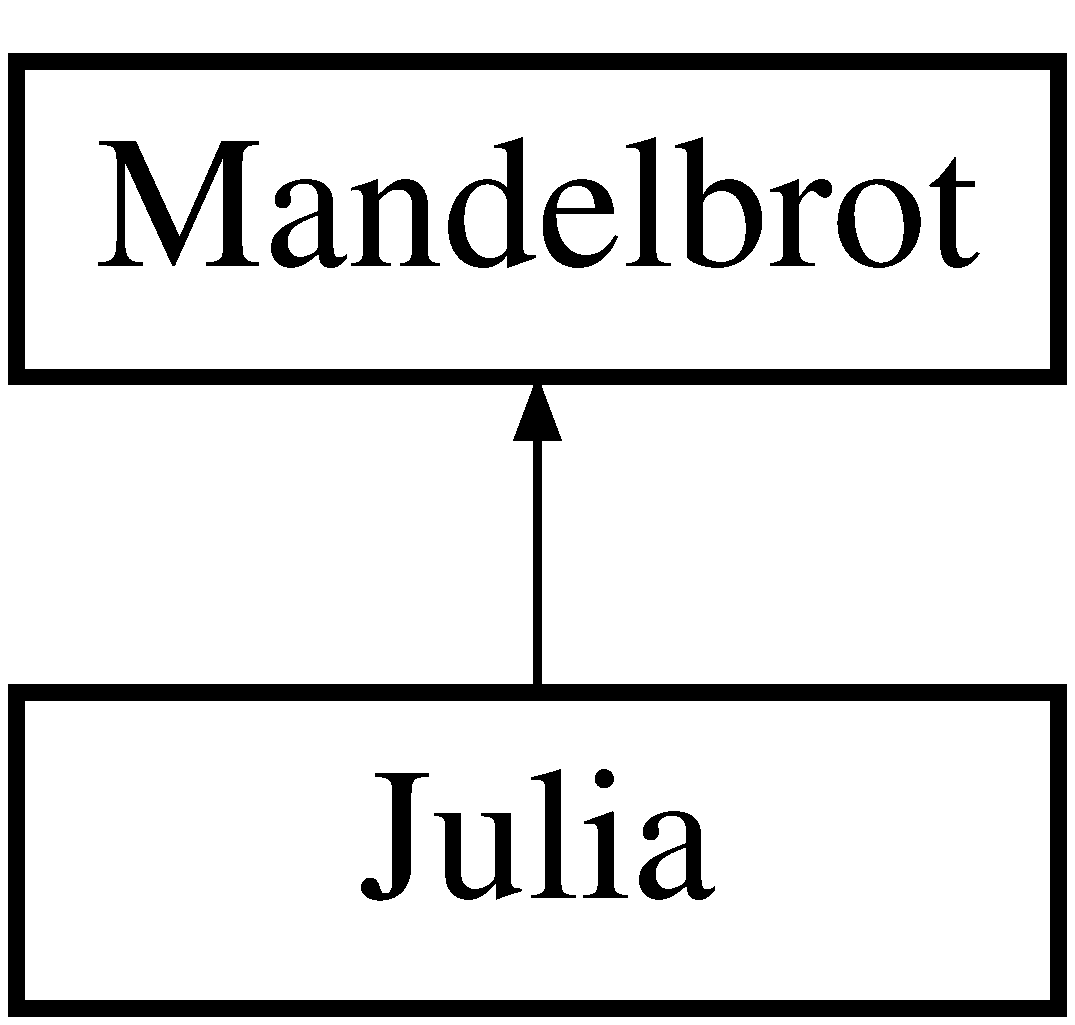
\includegraphics[height=2.000000cm]{class_julia}
\end{center}
\end{figure}
\subsection*{Public Member Functions}
\begin{DoxyCompactItemize}
\item 
\hyperlink{class_julia_a8bc853f8129d8f2503bbda1236f64b36}{Julia} (unsigned threads, unsigned depth)
\begin{DoxyCompactList}\small\item\em Explicitly constructs a \hyperlink{class_julia}{Julia} object. \end{DoxyCompactList}\item 
void \hyperlink{class_julia_ab877233424159ca87da6dcf0f0f36e51}{draw} (\hyperlink{classtsgl_1_1_cartesian_canvas}{Cart} \&can)
\begin{DoxyCompactList}\small\item\em Draw the \hyperlink{class_julia}{Julia} object. \end{DoxyCompactList}\end{DoxyCompactItemize}
\subsection*{Additional Inherited Members}


\subsection{Detailed Description}
Draw a \hyperlink{class_julia}{Julia} set. 

Contains all of the information necessary in order to draw a \hyperlink{class_julia}{Julia} set onto a Cartesian\+Canvas.

Can zoom in and out of the \hyperlink{class_julia}{Julia} set by scrolling the mouse wheel up and down (respectively).

Same is true when clicking the left mouse button (zooming in) and the right mouse button (zooming out).

Can also clear the screen by pressing the spacebar. 

\subsection{Constructor \& Destructor Documentation}
\mbox{\Hypertarget{class_julia_a8bc853f8129d8f2503bbda1236f64b36}\label{class_julia_a8bc853f8129d8f2503bbda1236f64b36}} 
\index{Julia@{Julia}!Julia@{Julia}}
\index{Julia@{Julia}!Julia@{Julia}}
\subsubsection{\texorpdfstring{Julia()}{Julia()}}
{\footnotesize\ttfamily Julia\+::\+Julia (\begin{DoxyParamCaption}\item[{unsigned}]{threads,  }\item[{unsigned}]{depth }\end{DoxyParamCaption})}



Explicitly constructs a \hyperlink{class_julia}{Julia} object. 

Explicit constructor for the \hyperlink{class_julia}{Julia} class. 
\begin{DoxyParams}{Parameters}
{\em threads} & The number of threads to use in drawing the \hyperlink{class_julia}{Julia} object onto the Cartesian\+Canvas. \\
\hline
{\em depth} & The number of iterations to go to in order to draw the \hyperlink{class_julia}{Julia} object. \\
\hline
\end{DoxyParams}
\begin{DoxyReturn}{Returns}
The constructed \hyperlink{class_julia}{Julia} object. 
\end{DoxyReturn}


\subsection{Member Function Documentation}
\mbox{\Hypertarget{class_julia_ab877233424159ca87da6dcf0f0f36e51}\label{class_julia_ab877233424159ca87da6dcf0f0f36e51}} 
\index{Julia@{Julia}!draw@{draw}}
\index{draw@{draw}!Julia@{Julia}}
\subsubsection{\texorpdfstring{draw()}{draw()}}
{\footnotesize\ttfamily void Julia\+::draw (\begin{DoxyParamCaption}\item[{\hyperlink{classtsgl_1_1_cartesian_canvas}{Cart} \&}]{can }\end{DoxyParamCaption})\hspace{0.3cm}{\ttfamily [virtual]}}



Draw the \hyperlink{class_julia}{Julia} object. 

Actually draws the \hyperlink{class_julia}{Julia} object to a Cartesian\+Canvas. 
\begin{DoxyParams}{Parameters}
{\em can} & Reference to the Cartesian\+Canvas to draw on. \\
\hline
\end{DoxyParams}
\begin{DoxyNote}{Note}
Cart is a typedef for a Cartesian\+Canvas object. 
\end{DoxyNote}


Reimplemented from \hyperlink{class_mandelbrot_ab7918e4de8f00f73290f110ca7a6cffd}{Mandelbrot}.



The documentation for this class was generated from the following files\+:\begin{DoxyCompactItemize}
\item 
/home/sth5/test/\+T\+S\+G\+L/src/examples/\+Mandelbrot/Julia.\+h\item 
/home/sth5/test/\+T\+S\+G\+L/src/examples/\+Mandelbrot/Julia.\+cpp\end{DoxyCompactItemize}

\hypertarget{class_langton_ant}{}\section{Langton\+Ant Class Reference}
\label{class_langton_ant}\index{Langton\+Ant@{Langton\+Ant}}


Create one of Langton\textquotesingle{}s Ant!  




{\ttfamily \#include $<$Langton\+Ant.\+h$>$}

\subsection*{Public Member Functions}
\begin{DoxyCompactItemize}
\item 
\hyperlink{class_langton_ant_ac3947796f9411f19c9dd547a1b89cf03}{Langton\+Ant} (int x, int y, int r, int g, int b, int d, \hyperlink{class_ant_farm}{Ant\+Farm} $\ast$p)
\begin{DoxyCompactList}\small\item\em Explicitly constructs a \hyperlink{class_langton_ant}{Langton\+Ant} object. \end{DoxyCompactList}\item 
void \hyperlink{class_langton_ant_acf17f14d78270a32b66273d83d8900c1}{move} ()
\begin{DoxyCompactList}\small\item\em Move the \hyperlink{class_langton_ant}{Langton\+Ant} object. \end{DoxyCompactList}\item 
void \hyperlink{class_langton_ant_ab5d2f1dc402bd5c6aa6552aad1ca50ca}{change\+Color} (int r, int g, int b)
\begin{DoxyCompactList}\small\item\em Change the color of a \hyperlink{class_langton_ant}{Langton\+Ant} object. \end{DoxyCompactList}\item 
void \hyperlink{class_langton_ant_a940dc3a5c0286ee91dd863ece7dc3998}{change\+Color} (\hyperlink{structtsgl_1_1_color_float}{Color\+Float} c)
\begin{DoxyCompactList}\small\item\em Change the color of a \hyperlink{class_langton_ant}{Langton\+Ant} object. \end{DoxyCompactList}\item 
void \hyperlink{class_langton_ant_a5fd5b25e776cfe96abe70300d022e333}{set\+Alpha} (int a)
\begin{DoxyCompactList}\small\item\em Set the alpha component of the color. \end{DoxyCompactList}\end{DoxyCompactItemize}
\subsection*{Public Attributes}
\begin{DoxyCompactItemize}
\item 
\mbox{\Hypertarget{class_langton_ant_afab907366d5000ba39ee0cded177110c}\label{class_langton_ant_afab907366d5000ba39ee0cded177110c}} 
int {\bfseries myX}
\item 
\mbox{\Hypertarget{class_langton_ant_aa7f6eccf65908ef06dc2453a6f4f4063}\label{class_langton_ant_aa7f6eccf65908ef06dc2453a6f4f4063}} 
int {\bfseries myY}
\item 
\mbox{\Hypertarget{class_langton_ant_abe7a992ac3e4a4ad14108dabc30c3ee2}\label{class_langton_ant_abe7a992ac3e4a4ad14108dabc30c3ee2}} 
int {\bfseries my\+Red}
\item 
\mbox{\Hypertarget{class_langton_ant_aad3f03053456bee3956a8358de57f109}\label{class_langton_ant_aad3f03053456bee3956a8358de57f109}} 
int {\bfseries my\+Green}
\item 
\mbox{\Hypertarget{class_langton_ant_a70481e24e34cbcaf46da72d5b9c13f56}\label{class_langton_ant_a70481e24e34cbcaf46da72d5b9c13f56}} 
int {\bfseries my\+Blue}
\item 
\mbox{\Hypertarget{class_langton_ant_ab5795182669f202beacb4abe6682629b}\label{class_langton_ant_ab5795182669f202beacb4abe6682629b}} 
int {\bfseries my\+Alpha}
\item 
\mbox{\Hypertarget{class_langton_ant_a62b83daa2325575e8079817fd8a416c5}\label{class_langton_ant_a62b83daa2325575e8079817fd8a416c5}} 
int {\bfseries my\+Dir}
\item 
\mbox{\Hypertarget{class_langton_ant_a814b5625591925045665f93f08eef3f4}\label{class_langton_ant_a814b5625591925045665f93f08eef3f4}} 
\hyperlink{class_ant_farm}{Ant\+Farm} $\ast$ {\bfseries my\+Farm}
\end{DoxyCompactItemize}


\subsection{Detailed Description}
Create one of Langton\textquotesingle{}s Ant! 

Contains all of the data and method needed in order to simulate a \hyperlink{class_langton_ant}{Langton\+Ant}.

You can change the color either by manually setting the red, green, and blue components or by passing a Color\+Float struct that contains those values.

The movement of each \hyperlink{class_langton_ant}{Langton\+Ant} is determined by its direction; UP, D\+O\+WN, L\+E\+FT, or R\+I\+G\+HT.

You can also set each \hyperlink{class_langton_ant}{Langton\+Ant} object to have an alpha value in order to make them transparent. 

\subsection{Constructor \& Destructor Documentation}
\mbox{\Hypertarget{class_langton_ant_ac3947796f9411f19c9dd547a1b89cf03}\label{class_langton_ant_ac3947796f9411f19c9dd547a1b89cf03}} 
\index{Langton\+Ant@{Langton\+Ant}!Langton\+Ant@{Langton\+Ant}}
\index{Langton\+Ant@{Langton\+Ant}!Langton\+Ant@{Langton\+Ant}}
\subsubsection{\texorpdfstring{Langton\+Ant()}{LangtonAnt()}}
{\footnotesize\ttfamily Langton\+Ant\+::\+Langton\+Ant (\begin{DoxyParamCaption}\item[{int}]{x,  }\item[{int}]{y,  }\item[{int}]{r,  }\item[{int}]{g,  }\item[{int}]{b,  }\item[{int}]{d,  }\item[{\hyperlink{class_ant_farm}{Ant\+Farm} $\ast$}]{p }\end{DoxyParamCaption})}



Explicitly constructs a \hyperlink{class_langton_ant}{Langton\+Ant} object. 

Explicit constructor for the \hyperlink{class_langton_ant}{Langton\+Ant} class. 
\begin{DoxyParams}{Parameters}
{\em x} & The x coordinate of the \hyperlink{class_langton_ant}{Langton\+Ant} object. \\
\hline
{\em y} & The y coordinate of the \hyperlink{class_langton_ant}{Langton\+Ant} object. \\
\hline
{\em r} & Red component for the color of the \hyperlink{class_langton_ant}{Langton\+Ant} object. \\
\hline
{\em g} & Green component for the color of the \hyperlink{class_langton_ant}{Langton\+Ant} object. \\
\hline
{\em b} & Blue component for the color of the \hyperlink{class_langton_ant}{Langton\+Ant} object. \\
\hline
{\em d} & The direction of the \hyperlink{class_langton_ant}{Langton\+Ant} object. \\
\hline
{\em p} & Pointer to the \hyperlink{class_ant_farm}{Ant\+Farm} object that the \hyperlink{class_langton_ant}{Langton\+Ant} object belongs to. \\
\hline
\end{DoxyParams}
\begin{DoxyReturn}{Returns}
The constructed \hyperlink{class_langton_ant}{Langton\+Ant} object. 
\end{DoxyReturn}


\subsection{Member Function Documentation}
\mbox{\Hypertarget{class_langton_ant_ab5d2f1dc402bd5c6aa6552aad1ca50ca}\label{class_langton_ant_ab5d2f1dc402bd5c6aa6552aad1ca50ca}} 
\index{Langton\+Ant@{Langton\+Ant}!change\+Color@{change\+Color}}
\index{change\+Color@{change\+Color}!Langton\+Ant@{Langton\+Ant}}
\subsubsection{\texorpdfstring{change\+Color()}{changeColor()}\hspace{0.1cm}{\footnotesize\ttfamily [1/2]}}
{\footnotesize\ttfamily void Langton\+Ant\+::change\+Color (\begin{DoxyParamCaption}\item[{int}]{r,  }\item[{int}]{g,  }\item[{int}]{b }\end{DoxyParamCaption})}



Change the color of a \hyperlink{class_langton_ant}{Langton\+Ant} object. 

Specifying a new red, green, and blue component allows you to change the color of the \hyperlink{class_langton_ant}{Langton\+Ant} object. 
\begin{DoxyParams}{Parameters}
{\em r} & Red component of the new color for the \hyperlink{class_langton_ant}{Langton\+Ant} object. \\
\hline
{\em g} & Green component of the new color for the \hyperlink{class_langton_ant}{Langton\+Ant} object. \\
\hline
{\em b} & Blue component of the new color for the Lanton\+Ant object. \\
\hline
\end{DoxyParams}


Referenced by change\+Color().

\mbox{\Hypertarget{class_langton_ant_a940dc3a5c0286ee91dd863ece7dc3998}\label{class_langton_ant_a940dc3a5c0286ee91dd863ece7dc3998}} 
\index{Langton\+Ant@{Langton\+Ant}!change\+Color@{change\+Color}}
\index{change\+Color@{change\+Color}!Langton\+Ant@{Langton\+Ant}}
\subsubsection{\texorpdfstring{change\+Color()}{changeColor()}\hspace{0.1cm}{\footnotesize\ttfamily [2/2]}}
{\footnotesize\ttfamily void Langton\+Ant\+::change\+Color (\begin{DoxyParamCaption}\item[{\hyperlink{structtsgl_1_1_color_float}{Color\+Float}}]{c }\end{DoxyParamCaption})}



Change the color of a \hyperlink{class_langton_ant}{Langton\+Ant} object. 

Same as change\+Color(r, g, b) but instead of passing the red, green, and blue components seperately you are passing a Color\+Float struct that contains all three. 
\begin{DoxyParams}{Parameters}
{\em c} & A Color\+Float struct containing the new red, green, and blue components for the new color of the \hyperlink{class_langton_ant}{Langton\+Ant} object. \\
\hline
\end{DoxyParams}
\mbox{\Hypertarget{class_langton_ant_acf17f14d78270a32b66273d83d8900c1}\label{class_langton_ant_acf17f14d78270a32b66273d83d8900c1}} 
\index{Langton\+Ant@{Langton\+Ant}!move@{move}}
\index{move@{move}!Langton\+Ant@{Langton\+Ant}}
\subsubsection{\texorpdfstring{move()}{move()}}
{\footnotesize\ttfamily void Langton\+Ant\+::move (\begin{DoxyParamCaption}{ }\end{DoxyParamCaption})}



Move the \hyperlink{class_langton_ant}{Langton\+Ant} object. 

Set to movement of the \hyperlink{class_langton_ant}{Langton\+Ant} object based off of its current direction (UP, D\+O\+WN, L\+E\+FT, or R\+I\+G\+HT). \mbox{\Hypertarget{class_langton_ant_a5fd5b25e776cfe96abe70300d022e333}\label{class_langton_ant_a5fd5b25e776cfe96abe70300d022e333}} 
\index{Langton\+Ant@{Langton\+Ant}!set\+Alpha@{set\+Alpha}}
\index{set\+Alpha@{set\+Alpha}!Langton\+Ant@{Langton\+Ant}}
\subsubsection{\texorpdfstring{set\+Alpha()}{setAlpha()}}
{\footnotesize\ttfamily void Langton\+Ant\+::set\+Alpha (\begin{DoxyParamCaption}\item[{int}]{a }\end{DoxyParamCaption})}



Set the alpha component of the color. 

Set the alpha component of the color for a \hyperlink{class_langton_ant}{Langton\+Ant} object. 
\begin{DoxyParams}{Parameters}
{\em a} & Alpha component to give to the \hyperlink{class_langton_ant}{Langton\+Ant} object. \\
\hline
\end{DoxyParams}


The documentation for this class was generated from the following files\+:\begin{DoxyCompactItemize}
\item 
/home/sth5/test/\+T\+S\+G\+L/src/examples/\+Langton/Langton\+Ant.\+h\item 
/home/sth5/test/\+T\+S\+G\+L/src/examples/\+Langton/Langton\+Ant.\+cpp\end{DoxyCompactItemize}

\hypertarget{class_life_farm}{}\section{Life\+Farm Class Reference}
\label{class_life_farm}\index{Life\+Farm@{Life\+Farm}}


Simulate Conway\textquotesingle{}s Game of Life!  




{\ttfamily \#include $<$Life\+Farm.\+h$>$}

\subsection*{Public Member Functions}
\begin{DoxyCompactItemize}
\item 
\hyperlink{class_life_farm_a3efbe8593fe83e366118f3fd6c5c2602}{Life\+Farm} (int w, int h, \hyperlink{classtsgl_1_1_canvas}{Canvas} $\ast$can, bool randomize)
\begin{DoxyCompactList}\small\item\em Explicitly constructs a \hyperlink{class_life_farm}{Life\+Farm} object. \end{DoxyCompactList}\item 
\hyperlink{class_life_farm_a364e73979cc9f09718273a65ab95fda1}{$\sim$\+Life\+Farm} ()
\begin{DoxyCompactList}\small\item\em Destroy a \hyperlink{class_life_farm}{Life\+Farm} object. \end{DoxyCompactList}\item 
void \hyperlink{class_life_farm_ac7ca1a0ae94a971bd04a699f99965b00}{add\+Ant} (int x, int y)
\begin{DoxyCompactList}\small\item\em Add an ant. \end{DoxyCompactList}\item 
void \hyperlink{class_life_farm_a3a7fdaa21bdc3d302960b3ea83be95df}{move\+Ants} ()
\begin{DoxyCompactList}\small\item\em Move the ants. \end{DoxyCompactList}\item 
void \hyperlink{class_life_farm_a4dce4424b7820fd64d7ec489a9606f87}{move\+Ants\+Old} ()
\begin{DoxyCompactList}\small\item\em Move the ants. \end{DoxyCompactList}\item 
void \hyperlink{class_life_farm_ab4dfccfcf0cb2ac83466223b8bb4c237}{move\+Ants\+New} ()
\begin{DoxyCompactList}\small\item\em Move the ants. \end{DoxyCompactList}\item 
void \hyperlink{class_life_farm_a90d784b157199edccf818ce3524a061a}{set\+Drawdead} (bool b)
\begin{DoxyCompactList}\small\item\em Draw \char`\"{}dead\char`\"{} ants. \end{DoxyCompactList}\item 
void \hyperlink{class_life_farm_aa23a45af1c6a7fd82d7fcca51d864487}{life} (int $\ast$current, int $\ast$fresh)
\begin{DoxyCompactList}\small\item\em Give life to the ants! \end{DoxyCompactList}\end{DoxyCompactItemize}
\subsection*{Public Attributes}
\begin{DoxyCompactItemize}
\item 
\mbox{\Hypertarget{class_life_farm_a2f484e44dc4df664a5f9a32761a19af9}\label{class_life_farm_a2f484e44dc4df664a5f9a32761a19af9}} 
int {\bfseries width}
\item 
\mbox{\Hypertarget{class_life_farm_a63e58d91a3f7aee59886f89fd0230c2d}\label{class_life_farm_a63e58d91a3f7aee59886f89fd0230c2d}} 
int {\bfseries height}
\item 
\mbox{\Hypertarget{class_life_farm_a1ef07c284a5a6c09670824a1feb258a0}\label{class_life_farm_a1ef07c284a5a6c09670824a1feb258a0}} 
int {\bfseries size}
\item 
\mbox{\Hypertarget{class_life_farm_a06cc91dafd92d6487e416cbec539df38}\label{class_life_farm_a06cc91dafd92d6487e416cbec539df38}} 
\hyperlink{classtsgl_1_1_canvas}{Canvas} $\ast$ {\bfseries can}
\end{DoxyCompactItemize}


\subsection{Detailed Description}
Simulate Conway\textquotesingle{}s Game of Life! 

Contains the data and methods needed in order to simulate Conway\textquotesingle{}s Game of Life.

see \href{https://en.wikipedia.org/wiki/Conway's_Game_of_Life}{\tt https\+://en.\+wikipedia.\+org/wiki/\+Conway\textquotesingle{}s\+\_\+\+Game\+\_\+of\+\_\+\+Life} for more details on what Conway\textquotesingle{}s Game of Life is. 

\subsection{Constructor \& Destructor Documentation}
\mbox{\Hypertarget{class_life_farm_a3efbe8593fe83e366118f3fd6c5c2602}\label{class_life_farm_a3efbe8593fe83e366118f3fd6c5c2602}} 
\index{Life\+Farm@{Life\+Farm}!Life\+Farm@{Life\+Farm}}
\index{Life\+Farm@{Life\+Farm}!Life\+Farm@{Life\+Farm}}
\subsubsection{\texorpdfstring{Life\+Farm()}{LifeFarm()}}
{\footnotesize\ttfamily Life\+Farm\+::\+Life\+Farm (\begin{DoxyParamCaption}\item[{int}]{w,  }\item[{int}]{h,  }\item[{\hyperlink{classtsgl_1_1_canvas}{Canvas} $\ast$}]{can,  }\item[{bool}]{randomize }\end{DoxyParamCaption})}



Explicitly constructs a \hyperlink{class_life_farm}{Life\+Farm} object. 

Explicit constructor for the \hyperlink{class_life_farm}{Life\+Farm} class. 
\begin{DoxyParams}{Parameters}
{\em w} & The width of the \hyperlink{class_life_farm}{Life\+Farm} object. \\
\hline
{\em h} & The height of the \hyperlink{class_life_farm}{Life\+Farm} object. \\
\hline
{\em can} & Pointer to the Canvas to draw to. \\
\hline
{\em randomize} & Determines if we should randomize the motion of the ants that are currently in the \hyperlink{class_life_farm}{Life\+Farm} object. \\
\hline
\end{DoxyParams}
\mbox{\Hypertarget{class_life_farm_a364e73979cc9f09718273a65ab95fda1}\label{class_life_farm_a364e73979cc9f09718273a65ab95fda1}} 
\index{Life\+Farm@{Life\+Farm}!````~Life\+Farm@{$\sim$\+Life\+Farm}}
\index{````~Life\+Farm@{$\sim$\+Life\+Farm}!Life\+Farm@{Life\+Farm}}
\subsubsection{\texorpdfstring{$\sim$\+Life\+Farm()}{~LifeFarm()}}
{\footnotesize\ttfamily Life\+Farm\+::$\sim$\+Life\+Farm (\begin{DoxyParamCaption}{ }\end{DoxyParamCaption})}



Destroy a \hyperlink{class_life_farm}{Life\+Farm} object. 

Destructor for the \hyperlink{class_life_farm}{Life\+Farm} class. \begin{DoxyReturn}{Returns}
Frees up any allocated memory to a \hyperlink{class_life_farm}{Life\+Farm} object. 
\end{DoxyReturn}


\subsection{Member Function Documentation}
\mbox{\Hypertarget{class_life_farm_ac7ca1a0ae94a971bd04a699f99965b00}\label{class_life_farm_ac7ca1a0ae94a971bd04a699f99965b00}} 
\index{Life\+Farm@{Life\+Farm}!add\+Ant@{add\+Ant}}
\index{add\+Ant@{add\+Ant}!Life\+Farm@{Life\+Farm}}
\subsubsection{\texorpdfstring{add\+Ant()}{addAnt()}}
{\footnotesize\ttfamily void Life\+Farm\+::add\+Ant (\begin{DoxyParamCaption}\item[{int}]{x,  }\item[{int}]{y }\end{DoxyParamCaption})}



Add an ant. 

Adds an ant to the \hyperlink{class_life_farm}{Life\+Farm} object. 
\begin{DoxyParams}{Parameters}
{\em x} & The x coordinate of the ant in the \hyperlink{class_life_farm}{Life\+Farm} object. \\
\hline
{\em y} & The y coordinate of the ant in the \hyperlink{class_life_farm}{Life\+Farm} object. \\
\hline
\end{DoxyParams}


Referenced by Life\+Farm(), and move\+Ants\+Old().

\mbox{\Hypertarget{class_life_farm_aa23a45af1c6a7fd82d7fcca51d864487}\label{class_life_farm_aa23a45af1c6a7fd82d7fcca51d864487}} 
\index{Life\+Farm@{Life\+Farm}!life@{life}}
\index{life@{life}!Life\+Farm@{Life\+Farm}}
\subsubsection{\texorpdfstring{life()}{life()}}
{\footnotesize\ttfamily void Life\+Farm\+::life (\begin{DoxyParamCaption}\item[{int $\ast$}]{current,  }\item[{int $\ast$}]{fresh }\end{DoxyParamCaption})}



Give life to the ants! 

Makes the ants come alive by keeping track of their current positions and next state positions. 
\begin{DoxyParams}{Parameters}
{\em $\ast$current} & A pointer to an array of current states that the ants are in during the game. \\
\hline
{\em $\ast$fresh} & A pointer to an array of next states that the ants are going to be in during the game. \\
\hline
\end{DoxyParams}


Referenced by move\+Ants\+New().

\mbox{\Hypertarget{class_life_farm_a3a7fdaa21bdc3d302960b3ea83be95df}\label{class_life_farm_a3a7fdaa21bdc3d302960b3ea83be95df}} 
\index{Life\+Farm@{Life\+Farm}!move\+Ants@{move\+Ants}}
\index{move\+Ants@{move\+Ants}!Life\+Farm@{Life\+Farm}}
\subsubsection{\texorpdfstring{move\+Ants()}{moveAnts()}}
{\footnotesize\ttfamily void Life\+Farm\+::move\+Ants (\begin{DoxyParamCaption}{ }\end{DoxyParamCaption})}



Move the ants. 

Move the ants that are currently in the \hyperlink{class_life_farm}{Life\+Farm} object. \begin{DoxyNote}{Note}
This method class \hyperlink{class_life_farm_a4dce4424b7820fd64d7ec489a9606f87}{move\+Ants\+Old()}. 
\end{DoxyNote}
\begin{DoxySeeAlso}{See also}
\hyperlink{class_life_farm_a4dce4424b7820fd64d7ec489a9606f87}{move\+Ants\+Old()} 
\end{DoxySeeAlso}
\mbox{\Hypertarget{class_life_farm_ab4dfccfcf0cb2ac83466223b8bb4c237}\label{class_life_farm_ab4dfccfcf0cb2ac83466223b8bb4c237}} 
\index{Life\+Farm@{Life\+Farm}!move\+Ants\+New@{move\+Ants\+New}}
\index{move\+Ants\+New@{move\+Ants\+New}!Life\+Farm@{Life\+Farm}}
\subsubsection{\texorpdfstring{move\+Ants\+New()}{moveAntsNew()}}
{\footnotesize\ttfamily void Life\+Farm\+::move\+Ants\+New (\begin{DoxyParamCaption}{ }\end{DoxyParamCaption})}



Move the ants. 

This method moves the ants around to new positions. \begin{DoxySeeAlso}{See also}
\hyperlink{class_life_farm_a4dce4424b7820fd64d7ec489a9606f87}{move\+Ants\+Old()} 
\end{DoxySeeAlso}
\mbox{\Hypertarget{class_life_farm_a4dce4424b7820fd64d7ec489a9606f87}\label{class_life_farm_a4dce4424b7820fd64d7ec489a9606f87}} 
\index{Life\+Farm@{Life\+Farm}!move\+Ants\+Old@{move\+Ants\+Old}}
\index{move\+Ants\+Old@{move\+Ants\+Old}!Life\+Farm@{Life\+Farm}}
\subsubsection{\texorpdfstring{move\+Ants\+Old()}{moveAntsOld()}}
{\footnotesize\ttfamily void Life\+Farm\+::move\+Ants\+Old (\begin{DoxyParamCaption}{ }\end{DoxyParamCaption})}



Move the ants. 

This method is called first in order to move the ants around in the \hyperlink{class_life_farm}{Life\+Farm} object. \begin{DoxySeeAlso}{See also}
\hyperlink{class_life_farm_ab4dfccfcf0cb2ac83466223b8bb4c237}{move\+Ants\+New()} 
\end{DoxySeeAlso}


Referenced by move\+Ants().

\mbox{\Hypertarget{class_life_farm_a90d784b157199edccf818ce3524a061a}\label{class_life_farm_a90d784b157199edccf818ce3524a061a}} 
\index{Life\+Farm@{Life\+Farm}!set\+Drawdead@{set\+Drawdead}}
\index{set\+Drawdead@{set\+Drawdead}!Life\+Farm@{Life\+Farm}}
\subsubsection{\texorpdfstring{set\+Drawdead()}{setDrawdead()}}
{\footnotesize\ttfamily void Life\+Farm\+::set\+Drawdead (\begin{DoxyParamCaption}\item[{bool}]{b }\end{DoxyParamCaption})}



Draw \char`\"{}dead\char`\"{} ants. 

Determines if we should draw ants that have \char`\"{}died\char`\"{} in the game. 
\begin{DoxyParams}{Parameters}
{\em b} & A boolean that determines if we should draw the dead ants or not. \\
\hline
\end{DoxyParams}


The documentation for this class was generated from the following files\+:\begin{DoxyCompactItemize}
\item 
/home/sth5/test/\+T\+S\+G\+L/src/examples/\+Conway/Life\+Farm.\+h\item 
/home/sth5/test/\+T\+S\+G\+L/src/examples/\+Conway/Life\+Farm.\+cpp\end{DoxyCompactItemize}

\hypertarget{classtsgl_1_1_line}{}\section{tsgl\+:\+:Line Class Reference}
\label{classtsgl_1_1_line}\index{tsgl\+::\+Line@{tsgl\+::\+Line}}


Draw a simple line.  




{\ttfamily \#include $<$Line.\+h$>$}

Inheritance diagram for tsgl\+:\+:Line\+:\begin{figure}[H]
\begin{center}
\leavevmode
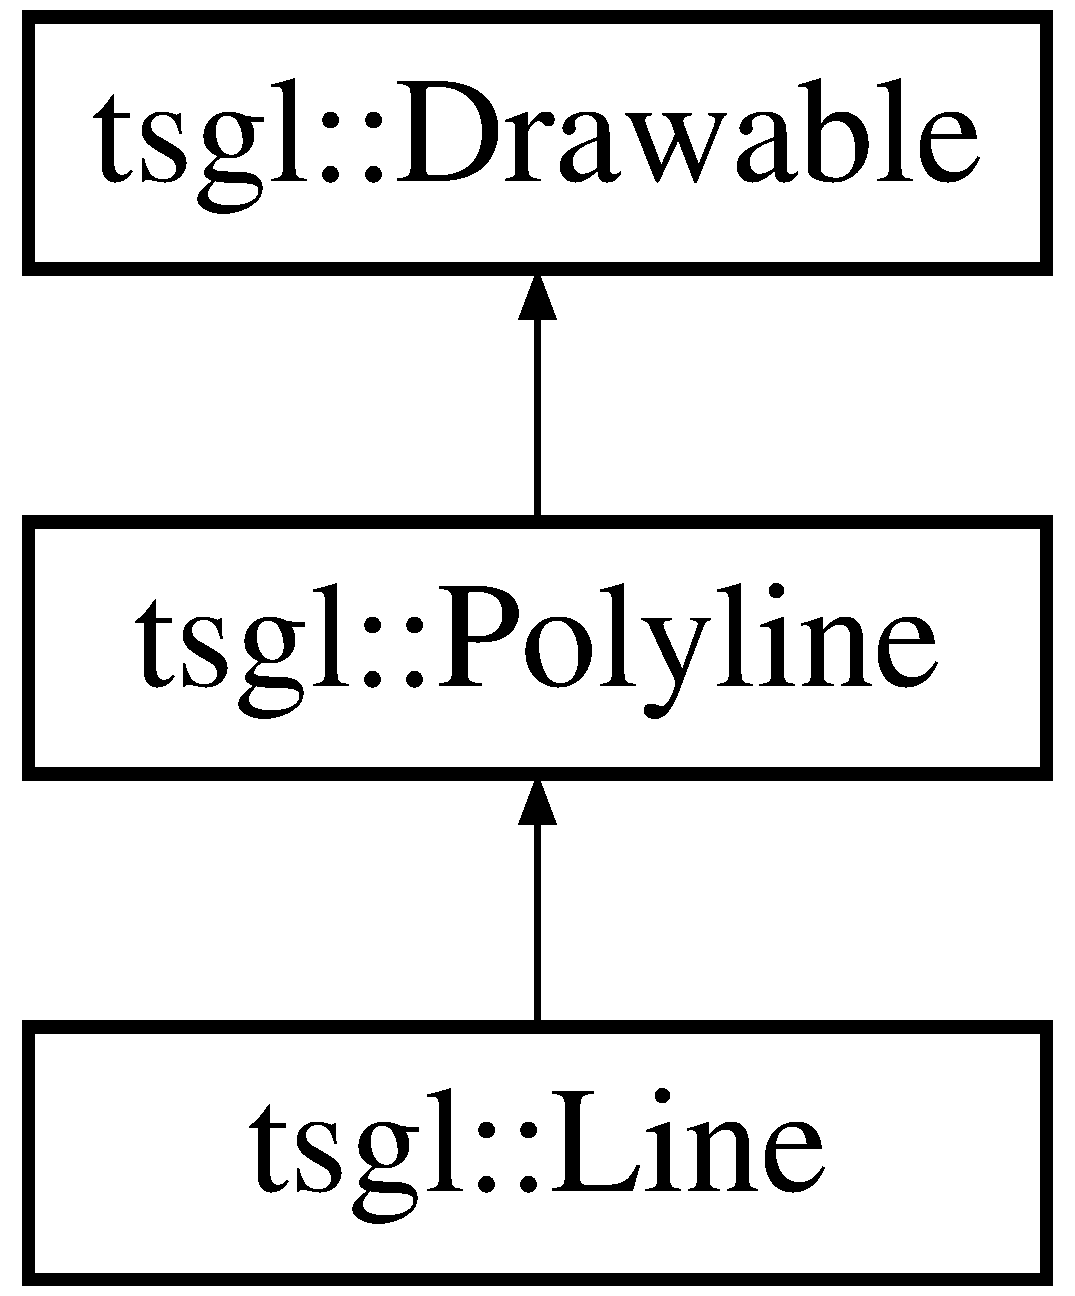
\includegraphics[height=2.000000cm]{classtsgl_1_1_line}
\end{center}
\end{figure}
\subsection*{Public Member Functions}
\begin{DoxyCompactItemize}
\item 
\hyperlink{classtsgl_1_1_line_af16488259ac5978679e13d58cf7e91ef}{Line} (int x1, int y1, int x2, int y2, const \hyperlink{structtsgl_1_1_color_float}{Color\+Float} \&color)
\begin{DoxyCompactList}\small\item\em Explicitly constructs a new \hyperlink{classtsgl_1_1_line}{Line}. \end{DoxyCompactList}\item 
void \hyperlink{classtsgl_1_1_line_ae7eccbbf5230a4c68139560d810af415}{draw} ()
\begin{DoxyCompactList}\small\item\em Draw the \hyperlink{classtsgl_1_1_line}{Line}. \end{DoxyCompactList}\end{DoxyCompactItemize}
\subsection*{Additional Inherited Members}


\subsection{Detailed Description}
Draw a simple line. 

\hyperlink{classtsgl_1_1_line}{Line} is a class for holding vertex data for a simple line. 

\subsection{Constructor \& Destructor Documentation}
\hypertarget{classtsgl_1_1_line_af16488259ac5978679e13d58cf7e91ef}{}\index{tsgl\+::\+Line@{tsgl\+::\+Line}!Line@{Line}}
\index{Line@{Line}!tsgl\+::\+Line@{tsgl\+::\+Line}}
\subsubsection[{Line}]{\setlength{\rightskip}{0pt plus 5cm}tsgl\+::\+Line\+::\+Line (
\begin{DoxyParamCaption}
\item[{int}]{x1, }
\item[{int}]{y1, }
\item[{int}]{x2, }
\item[{int}]{y2, }
\item[{const {\bf Color\+Float} \&}]{color}
\end{DoxyParamCaption}
)}\label{classtsgl_1_1_line_af16488259ac5978679e13d58cf7e91ef}


Explicitly constructs a new \hyperlink{classtsgl_1_1_line}{Line}. 

This is the constructor for the \hyperlink{classtsgl_1_1_line}{Line} class. 
\begin{DoxyParams}{Parameters}
{\em x1} & The x coordinate of the first endpoint. \\
\hline
{\em y1} & The y coordinate of the first endpoint. \\
\hline
{\em x2} & The x coordinate of the second endpoint. \\
\hline
{\em y2} & The y coordinate of the second endpoint. \\
\hline
{\em color} & The reference variable to the color of the \hyperlink{classtsgl_1_1_line}{Line}. \\
\hline
\end{DoxyParams}
\begin{DoxyReturn}{Returns}
A new \hyperlink{classtsgl_1_1_line}{Line} with the specified endpoints and color. 
\end{DoxyReturn}


\subsection{Member Function Documentation}
\hypertarget{classtsgl_1_1_line_ae7eccbbf5230a4c68139560d810af415}{}\index{tsgl\+::\+Line@{tsgl\+::\+Line}!draw@{draw}}
\index{draw@{draw}!tsgl\+::\+Line@{tsgl\+::\+Line}}
\subsubsection[{draw}]{\setlength{\rightskip}{0pt plus 5cm}void tsgl\+::\+Line\+::draw (
\begin{DoxyParamCaption}
{}
\end{DoxyParamCaption}
)\hspace{0.3cm}{\ttfamily [virtual]}}\label{classtsgl_1_1_line_ae7eccbbf5230a4c68139560d810af415}


Draw the \hyperlink{classtsgl_1_1_line}{Line}. 

This function actually draws the \hyperlink{classtsgl_1_1_line}{Line} to the \hyperlink{classtsgl_1_1_canvas}{Canvas}. 

Implements \hyperlink{classtsgl_1_1_shape_af78b1627b97d621824ce86db214e2402}{tsgl\+::\+Shape}.



The documentation for this class was generated from the following files\+:\begin{DoxyCompactItemize}
\item 
Line.\+h\item 
Line.\+cpp\end{DoxyCompactItemize}

\hypertarget{class_lock}{}\section{Lock Class Reference}
\label{class_lock}\index{Lock@{Lock}}


An abstract database protecting a vector of data.  




{\ttfamily \#include $<$Lock.\+h$>$}

Inheritance diagram for Lock\+:\begin{figure}[H]
\begin{center}
\leavevmode
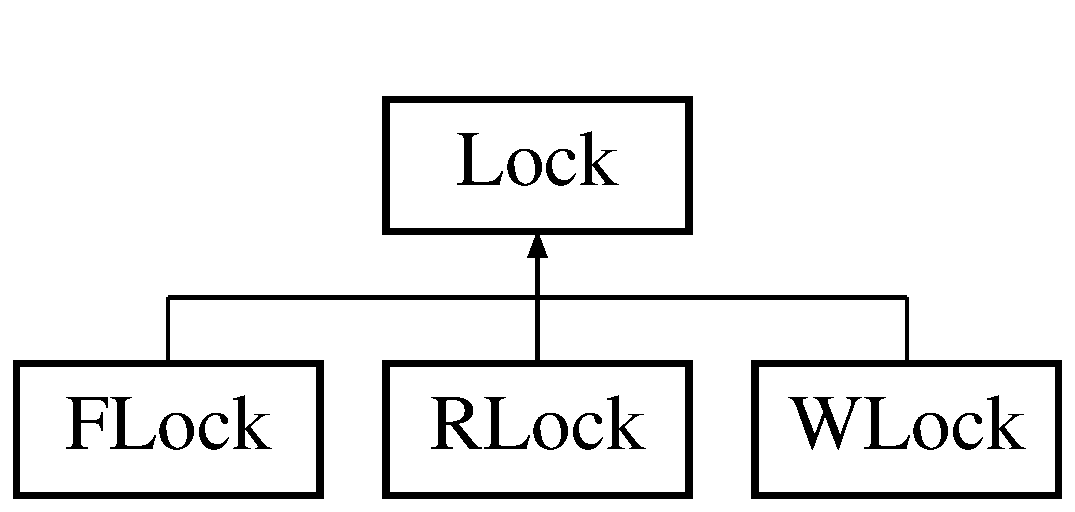
\includegraphics[height=2.000000cm]{class_lock}
\end{center}
\end{figure}
\subsection*{Public Member Functions}
\begin{DoxyCompactItemize}
\item 
\hyperlink{class_lock_a9944623567d8138b95e74fadc7190adb}{Lock} ()
\begin{DoxyCompactList}\small\item\em Default constructor for the \hyperlink{class_lock}{Lock} class. \end{DoxyCompactList}\item 
\hyperlink{class_lock_a6e5be419fc8b9db7b8c599e805634083}{Lock} (\hyperlink{class_r_w_database}{R\+W\+Database}$<$ \hyperlink{classtsgl_1_1_rectangle}{tsgl\+::\+Rectangle} $\ast$$>$ $\ast$data)
\begin{DoxyCompactList}\small\item\em Explicit constructor for the \hyperlink{class_lock}{Lock} class. \end{DoxyCompactList}\item 
\mbox{\Hypertarget{class_lock_ac92ae45f564598eefd51798c516f061c}\label{class_lock_ac92ae45f564598eefd51798c516f061c}} 
virtual void {\bfseries read\+Lock} ()=0
\item 
\mbox{\Hypertarget{class_lock_a6b58887c869c252cc4b396ea52770506}\label{class_lock_a6b58887c869c252cc4b396ea52770506}} 
virtual void {\bfseries read\+Unlock} ()=0
\item 
\mbox{\Hypertarget{class_lock_a9c95a05d9c8f1ea00d9242d3a73e8469}\label{class_lock_a9c95a05d9c8f1ea00d9242d3a73e8469}} 
virtual void {\bfseries write\+Lock} ()=0
\item 
\mbox{\Hypertarget{class_lock_a5940100b94c721324740c83669f0b322}\label{class_lock_a5940100b94c721324740c83669f0b322}} 
virtual void {\bfseries write\+Unlock} ()=0
\end{DoxyCompactItemize}
\subsection*{Protected Attributes}
\begin{DoxyCompactItemize}
\item 
\mbox{\Hypertarget{class_lock_ad69e84777545706182e74a890303fe86}\label{class_lock_ad69e84777545706182e74a890303fe86}} 
int {\bfseries active\+Writers}
\item 
\mbox{\Hypertarget{class_lock_ab826b5e8650fb5028756b1b189470446}\label{class_lock_ab826b5e8650fb5028756b1b189470446}} 
int {\bfseries active\+Readers}
\item 
\mbox{\Hypertarget{class_lock_aebab758da5c666817aa2a3cae2b7e7cc}\label{class_lock_aebab758da5c666817aa2a3cae2b7e7cc}} 
int {\bfseries waiting\+Writers}
\item 
\mbox{\Hypertarget{class_lock_a6a79d1a4a2ca7c9a5db7150c2775b4b3}\label{class_lock_a6a79d1a4a2ca7c9a5db7150c2775b4b3}} 
int {\bfseries waiting\+Readers}
\item 
\mbox{\Hypertarget{class_lock_a71ad42fa0f867c563c36d0e6fd265d66}\label{class_lock_a71ad42fa0f867c563c36d0e6fd265d66}} 
pthread\+\_\+mutex\+\_\+t {\bfseries lock}
\item 
\mbox{\Hypertarget{class_lock_ad3f154d852d212a46697c9f1d4ec9c16}\label{class_lock_ad3f154d852d212a46697c9f1d4ec9c16}} 
pthread\+\_\+cond\+\_\+t {\bfseries ok\+To\+Read}
\item 
\mbox{\Hypertarget{class_lock_a236095b855dabe05d173ee913bd9d876}\label{class_lock_a236095b855dabe05d173ee913bd9d876}} 
pthread\+\_\+cond\+\_\+t {\bfseries ok\+To\+Write}
\item 
\mbox{\Hypertarget{class_lock_ac05707ecf7e23343a78add6be3212861}\label{class_lock_ac05707ecf7e23343a78add6be3212861}} 
\hyperlink{class_r_w_database}{R\+W\+Database}$<$ \hyperlink{classtsgl_1_1_rectangle}{tsgl\+::\+Rectangle} $\ast$ $>$ $\ast$ {\bfseries data}
\end{DoxyCompactItemize}


\subsection{Detailed Description}
An abstract database protecting a vector of data. 

Database has its locks

Locking methods must be implemented in subclass, giving priority to different types of threads. 

\subsection{Constructor \& Destructor Documentation}
\mbox{\Hypertarget{class_lock_a9944623567d8138b95e74fadc7190adb}\label{class_lock_a9944623567d8138b95e74fadc7190adb}} 
\index{Lock@{Lock}!Lock@{Lock}}
\index{Lock@{Lock}!Lock@{Lock}}
\subsubsection{\texorpdfstring{Lock()}{Lock()}\hspace{0.1cm}{\footnotesize\ttfamily [1/2]}}
{\footnotesize\ttfamily Lock\+::\+Lock (\begin{DoxyParamCaption}{ }\end{DoxyParamCaption})}



Default constructor for the \hyperlink{class_lock}{Lock} class. 

Lock.\+cpp provides a \hyperlink{class_lock}{Lock} class for the Reader-\/\+Writer visualization. This class provides a superclass for the monitors with \hyperlink{class_reader}{Reader} or \hyperlink{class_writer}{Writer} preference, which are used by the threads. \begin{DoxyReturn}{Returns}
\+: The constructed \hyperlink{class_lock}{Lock} object. 
\end{DoxyReturn}


Referenced by F\+Lock\+::\+F\+Lock().

\mbox{\Hypertarget{class_lock_a6e5be419fc8b9db7b8c599e805634083}\label{class_lock_a6e5be419fc8b9db7b8c599e805634083}} 
\index{Lock@{Lock}!Lock@{Lock}}
\index{Lock@{Lock}!Lock@{Lock}}
\subsubsection{\texorpdfstring{Lock()}{Lock()}\hspace{0.1cm}{\footnotesize\ttfamily [2/2]}}
{\footnotesize\ttfamily Lock\+::\+Lock (\begin{DoxyParamCaption}\item[{\hyperlink{class_r_w_database}{R\+W\+Database}$<$ \hyperlink{classtsgl_1_1_rectangle}{tsgl\+::\+Rectangle} $\ast$$>$ $\ast$}]{database }\end{DoxyParamCaption})}



Explicit constructor for the \hyperlink{class_lock}{Lock} class. 


\begin{DoxyParams}{Parameters}
{\em data,the} & database being protected \\
\hline
\end{DoxyParams}
\begin{DoxyReturn}{Returns}
\+: The constructed \hyperlink{class_lock}{Lock} object. 
\end{DoxyReturn}


The documentation for this class was generated from the following files\+:\begin{DoxyCompactItemize}
\item 
/home/sth5/test/\+T\+S\+G\+L/src/examples/\+Reader\+Writer/Lock.\+h\item 
/home/sth5/test/\+T\+S\+G\+L/src/examples/\+Reader\+Writer/Lock.\+cpp\end{DoxyCompactItemize}

\hypertarget{class_mandelbrot}{}\section{Mandelbrot Class Reference}
\label{class_mandelbrot}\index{Mandelbrot@{Mandelbrot}}


Draw a \hyperlink{class_mandelbrot}{Mandelbrot} set.  




{\ttfamily \#include $<$Mandelbrot.\+h$>$}

Inheritance diagram for Mandelbrot\+:\begin{figure}[H]
\begin{center}
\leavevmode
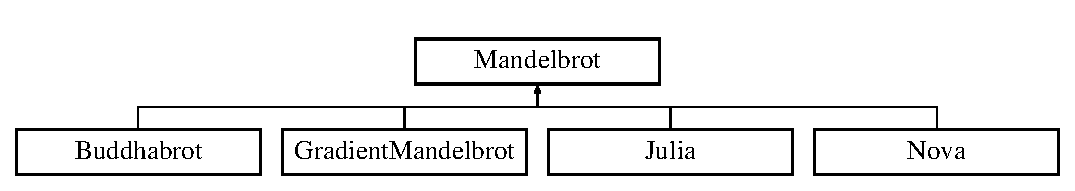
\includegraphics[height=2.000000cm]{class_mandelbrot}
\end{center}
\end{figure}
\subsection*{Public Member Functions}
\begin{DoxyCompactItemize}
\item 
\hyperlink{class_mandelbrot_ae0c71b1d8894206cb896412ae2fa1529}{Mandelbrot} (unsigned threads, unsigned depth)
\begin{DoxyCompactList}\small\item\em Explicitly construct a \hyperlink{class_mandelbrot}{Mandelbrot} object. \end{DoxyCompactList}\item 
virtual \hyperlink{class_mandelbrot_a886df208f291f5d24d7f8f582962bb84}{$\sim$\+Mandelbrot} ()
\begin{DoxyCompactList}\small\item\em Destroys a \hyperlink{class_mandelbrot}{Mandelbrot} object and any children of the \hyperlink{class_mandelbrot}{Mandelbrot} class. \end{DoxyCompactList}\item 
void \hyperlink{class_mandelbrot_a4b50829db11e2642b616431ae4e2eacf}{bindings} (\hyperlink{classtsgl_1_1_cartesian_canvas}{Cart} \&can)
\begin{DoxyCompactList}\small\item\em Binds buttons and/or mouse clicks. \end{DoxyCompactList}\item 
virtual void \hyperlink{class_mandelbrot_ab7918e4de8f00f73290f110ca7a6cffd}{draw} (\hyperlink{classtsgl_1_1_cartesian_canvas}{Cart} \&can)
\begin{DoxyCompactList}\small\item\em Draw the \hyperlink{class_mandelbrot}{Mandelbrot} object. \end{DoxyCompactList}\end{DoxyCompactItemize}
\subsection*{Protected Member Functions}
\begin{DoxyCompactItemize}
\item 
void \hyperlink{class_mandelbrot_aef094f9bb9b2fd1107481b150205ff53}{manhattan\+Shading} (\hyperlink{classtsgl_1_1_cartesian_canvas}{Cartesian\+Canvas} \&can)
\begin{DoxyCompactList}\small\item\em Shades the fractal using Manhattan distances. \end{DoxyCompactList}\end{DoxyCompactItemize}
\subsection*{Protected Attributes}
\begin{DoxyCompactItemize}
\item 
\mbox{\Hypertarget{class_mandelbrot_a41edcc618b65717d6511afb9f6e6031a}\label{class_mandelbrot_a41edcc618b65717d6511afb9f6e6031a}} 
int {\bfseries my\+Threads}
\item 
\mbox{\Hypertarget{class_mandelbrot_ae42189a68d6c97ba7614888eb20f07f0}\label{class_mandelbrot_ae42189a68d6c97ba7614888eb20f07f0}} 
unsigned int {\bfseries my\+Depth}
\item 
\mbox{\Hypertarget{class_mandelbrot_a3c79bfb1dd830a8d4d8f766a5bec83a4}\label{class_mandelbrot_a3c79bfb1dd830a8d4d8f766a5bec83a4}} 
bool {\bfseries my\+Redraw}
\end{DoxyCompactItemize}


\subsection{Detailed Description}
Draw a \hyperlink{class_mandelbrot}{Mandelbrot} set. 

Contains the information necessary in order to draw a \hyperlink{class_mandelbrot}{Mandelbrot} set onto a Cartesian\+Canvas.

Can zoom in and out of the screen by scrolling up and down on the mouse wheel (respectively).

Same is true if you click on the left mouse button (zoom in) and right mouse button (zoom out). 

\subsection{Constructor \& Destructor Documentation}
\mbox{\Hypertarget{class_mandelbrot_ae0c71b1d8894206cb896412ae2fa1529}\label{class_mandelbrot_ae0c71b1d8894206cb896412ae2fa1529}} 
\index{Mandelbrot@{Mandelbrot}!Mandelbrot@{Mandelbrot}}
\index{Mandelbrot@{Mandelbrot}!Mandelbrot@{Mandelbrot}}
\subsubsection{\texorpdfstring{Mandelbrot()}{Mandelbrot()}}
{\footnotesize\ttfamily Mandelbrot\+::\+Mandelbrot (\begin{DoxyParamCaption}\item[{unsigned}]{threads,  }\item[{unsigned}]{depth }\end{DoxyParamCaption})}



Explicitly construct a \hyperlink{class_mandelbrot}{Mandelbrot} object. 

Explicit constructor for the \hyperlink{class_mandelbrot}{Mandelbrot} class. 
\begin{DoxyParams}{Parameters}
{\em threads} & The number of threads to use in drawing the \hyperlink{class_mandelbrot}{Mandelbrot} object onto the Cartesian\+Canvas. \\
\hline
{\em depth} & The number of iterations to go to in order to draw the \hyperlink{class_mandelbrot}{Mandelbrot} object. \\
\hline
\end{DoxyParams}
\begin{DoxyReturn}{Returns}
The constructed \hyperlink{class_mandelbrot}{Mandelbrot} object. 
\end{DoxyReturn}
\mbox{\Hypertarget{class_mandelbrot_a886df208f291f5d24d7f8f582962bb84}\label{class_mandelbrot_a886df208f291f5d24d7f8f582962bb84}} 
\index{Mandelbrot@{Mandelbrot}!````~Mandelbrot@{$\sim$\+Mandelbrot}}
\index{````~Mandelbrot@{$\sim$\+Mandelbrot}!Mandelbrot@{Mandelbrot}}
\subsubsection{\texorpdfstring{$\sim$\+Mandelbrot()}{~Mandelbrot()}}
{\footnotesize\ttfamily virtual Mandelbrot\+::$\sim$\+Mandelbrot (\begin{DoxyParamCaption}{ }\end{DoxyParamCaption})\hspace{0.3cm}{\ttfamily [inline]}, {\ttfamily [virtual]}}



Destroys a \hyperlink{class_mandelbrot}{Mandelbrot} object and any children of the \hyperlink{class_mandelbrot}{Mandelbrot} class. 

Destructor for the \hyperlink{class_mandelbrot}{Mandelbrot} class and its children. \begin{DoxyNote}{Note}
Does absolutely nothing. 
\end{DoxyNote}


\subsection{Member Function Documentation}
\mbox{\Hypertarget{class_mandelbrot_a4b50829db11e2642b616431ae4e2eacf}\label{class_mandelbrot_a4b50829db11e2642b616431ae4e2eacf}} 
\index{Mandelbrot@{Mandelbrot}!bindings@{bindings}}
\index{bindings@{bindings}!Mandelbrot@{Mandelbrot}}
\subsubsection{\texorpdfstring{bindings()}{bindings()}}
{\footnotesize\ttfamily void Mandelbrot\+::bindings (\begin{DoxyParamCaption}\item[{\hyperlink{classtsgl_1_1_cartesian_canvas}{Cart} \&}]{can }\end{DoxyParamCaption})}



Binds buttons and/or mouse clicks. 

Binds buttons and/or mouse clicks needed for I/O capabilities.

In this case\+: the mouse wheel, left and right mouse buttons. 
\begin{DoxyParams}{Parameters}
{\em can} & Reference to the Cartesian\+Canvas to have the buttons bound to. \\
\hline
\end{DoxyParams}
\begin{DoxyNote}{Note}
Cart is a typedef for Cartesian\+Canvas. 
\end{DoxyNote}
\mbox{\Hypertarget{class_mandelbrot_ab7918e4de8f00f73290f110ca7a6cffd}\label{class_mandelbrot_ab7918e4de8f00f73290f110ca7a6cffd}} 
\index{Mandelbrot@{Mandelbrot}!draw@{draw}}
\index{draw@{draw}!Mandelbrot@{Mandelbrot}}
\subsubsection{\texorpdfstring{draw()}{draw()}}
{\footnotesize\ttfamily void Mandelbrot\+::draw (\begin{DoxyParamCaption}\item[{\hyperlink{classtsgl_1_1_cartesian_canvas}{Cart} \&}]{can }\end{DoxyParamCaption})\hspace{0.3cm}{\ttfamily [virtual]}}



Draw the \hyperlink{class_mandelbrot}{Mandelbrot} object. 

Actually draws the \hyperlink{class_mandelbrot}{Mandelbrot} object onto the Cartesian\+Canvas. 
\begin{DoxyParams}{Parameters}
{\em can} & Reference to the Cartesian\+Canvas to draw on. \\
\hline
\end{DoxyParams}
\begin{DoxyNote}{Note}
Can be inherited by children classes who extend the \hyperlink{class_mandelbrot}{Mandelbrot} class. 

Cart is a typedef for Cartesian\+Canvas. 
\end{DoxyNote}


Reimplemented in \hyperlink{class_buddhabrot_a9e65eb7e2cac8737aedec56a7e2c274c}{Buddhabrot}, \hyperlink{class_gradient_mandelbrot_a1d4aa3e44d7d1c2241545b60c79985df}{Gradient\+Mandelbrot}, \hyperlink{class_julia_ab877233424159ca87da6dcf0f0f36e51}{Julia}, and \hyperlink{class_nova_a66935ba0814dfabcae2481c128c336ec}{Nova}.

\mbox{\Hypertarget{class_mandelbrot_aef094f9bb9b2fd1107481b150205ff53}\label{class_mandelbrot_aef094f9bb9b2fd1107481b150205ff53}} 
\index{Mandelbrot@{Mandelbrot}!manhattan\+Shading@{manhattan\+Shading}}
\index{manhattan\+Shading@{manhattan\+Shading}!Mandelbrot@{Mandelbrot}}
\subsubsection{\texorpdfstring{manhattan\+Shading()}{manhattanShading()}}
{\footnotesize\ttfamily void Mandelbrot\+::manhattan\+Shading (\begin{DoxyParamCaption}\item[{\hyperlink{classtsgl_1_1_cartesian_canvas}{Cartesian\+Canvas} \&}]{can }\end{DoxyParamCaption})\hspace{0.3cm}{\ttfamily [protected]}}



Shades the fractal using Manhattan distances. 

This function may be called after the \hyperlink{class_mandelbrot}{Mandelbrot} has finished rendering to do some post-\/procecssing using the distances from non-\/escaped pixels to their nearest escaped pixels, using the average of their Manhattan distances. 

Referenced by Nova\+::draw().



The documentation for this class was generated from the following files\+:\begin{DoxyCompactItemize}
\item 
/home/sth5/test/\+T\+S\+G\+L/src/examples/\+Mandelbrot/Mandelbrot.\+h\item 
/home/sth5/test/\+T\+S\+G\+L/src/examples/\+Mandelbrot/Mandelbrot.\+cpp\end{DoxyCompactItemize}

\hypertarget{classtsgl_1_1_natural_log_function}{}\section{tsgl\+:\+:Natural\+Log\+Function Class Reference}
\label{classtsgl_1_1_natural_log_function}\index{tsgl\+::\+Natural\+Log\+Function@{tsgl\+::\+Natural\+Log\+Function}}


\hyperlink{classtsgl_1_1_function}{Function} to compute the natural log of the input.  




{\ttfamily \#include $<$Function.\+h$>$}

Inheritance diagram for tsgl\+:\+:Natural\+Log\+Function\+:\begin{figure}[H]
\begin{center}
\leavevmode
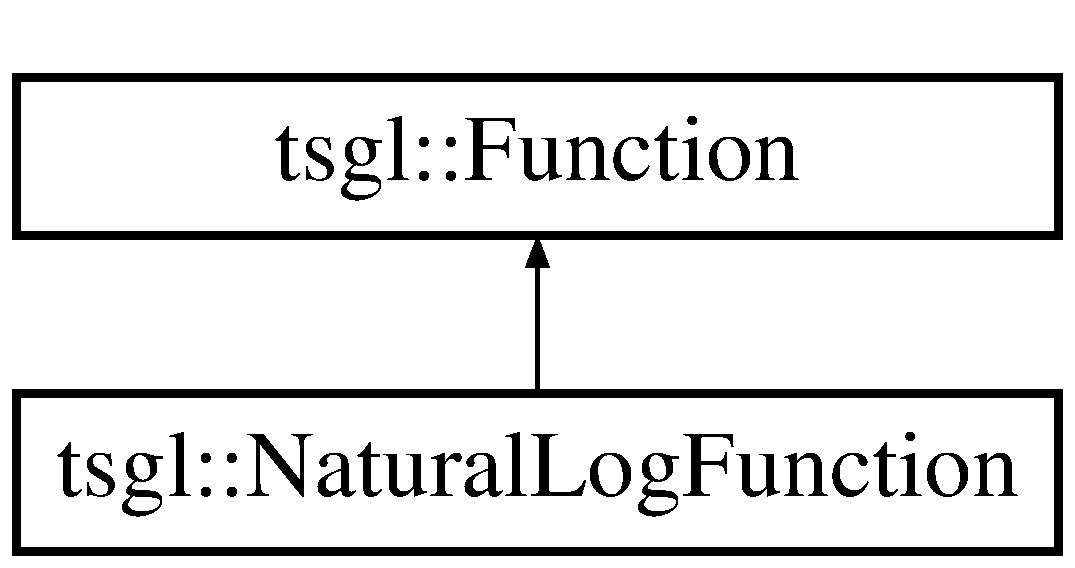
\includegraphics[height=2.000000cm]{classtsgl_1_1_natural_log_function}
\end{center}
\end{figure}
\subsection*{Public Member Functions}
\begin{DoxyCompactItemize}
\item 
virtual Decimal \hyperlink{classtsgl_1_1_natural_log_function_a21ce8c1cad8b13dccf9308c73a48df12}{value\+At} (Decimal x) const 
\begin{DoxyCompactList}\small\item\em Method to determine the value of \hyperlink{classtsgl_1_1_natural_log_function}{Natural\+Log\+Function}. \end{DoxyCompactList}\end{DoxyCompactItemize}


\subsection{Detailed Description}
\hyperlink{classtsgl_1_1_function}{Function} to compute the natural log of the input. 

\subsection{Member Function Documentation}
\hypertarget{classtsgl_1_1_natural_log_function_a21ce8c1cad8b13dccf9308c73a48df12}{}\index{tsgl\+::\+Natural\+Log\+Function@{tsgl\+::\+Natural\+Log\+Function}!value\+At@{value\+At}}
\index{value\+At@{value\+At}!tsgl\+::\+Natural\+Log\+Function@{tsgl\+::\+Natural\+Log\+Function}}
\subsubsection[{value\+At}]{\setlength{\rightskip}{0pt plus 5cm}virtual Decimal tsgl\+::\+Natural\+Log\+Function\+::value\+At (
\begin{DoxyParamCaption}
\item[{Decimal}]{x}
\end{DoxyParamCaption}
) const\hspace{0.3cm}{\ttfamily [inline]}, {\ttfamily [virtual]}}\label{classtsgl_1_1_natural_log_function_a21ce8c1cad8b13dccf9308c73a48df12}


Method to determine the value of \hyperlink{classtsgl_1_1_natural_log_function}{Natural\+Log\+Function}. 

\begin{DoxyReturn}{Returns}
The natural log of {\itshape x}. 
\end{DoxyReturn}


Implements \hyperlink{classtsgl_1_1_function_affb7b3b19a04efefa29a9870d666e912}{tsgl\+::\+Function}.



The documentation for this class was generated from the following file\+:\begin{DoxyCompactItemize}
\item 
Function.\+h\end{DoxyCompactItemize}

\hypertarget{class_nova}{}\section{Nova Class Reference}
\label{class_nova}\index{Nova@{Nova}}


Draws a \hyperlink{class_nova}{Nova} (Newton Fractal) set on a Cartesian\+Canvas.  




{\ttfamily \#include $<$Nova.\+h$>$}

Inheritance diagram for Nova\+:\begin{figure}[H]
\begin{center}
\leavevmode
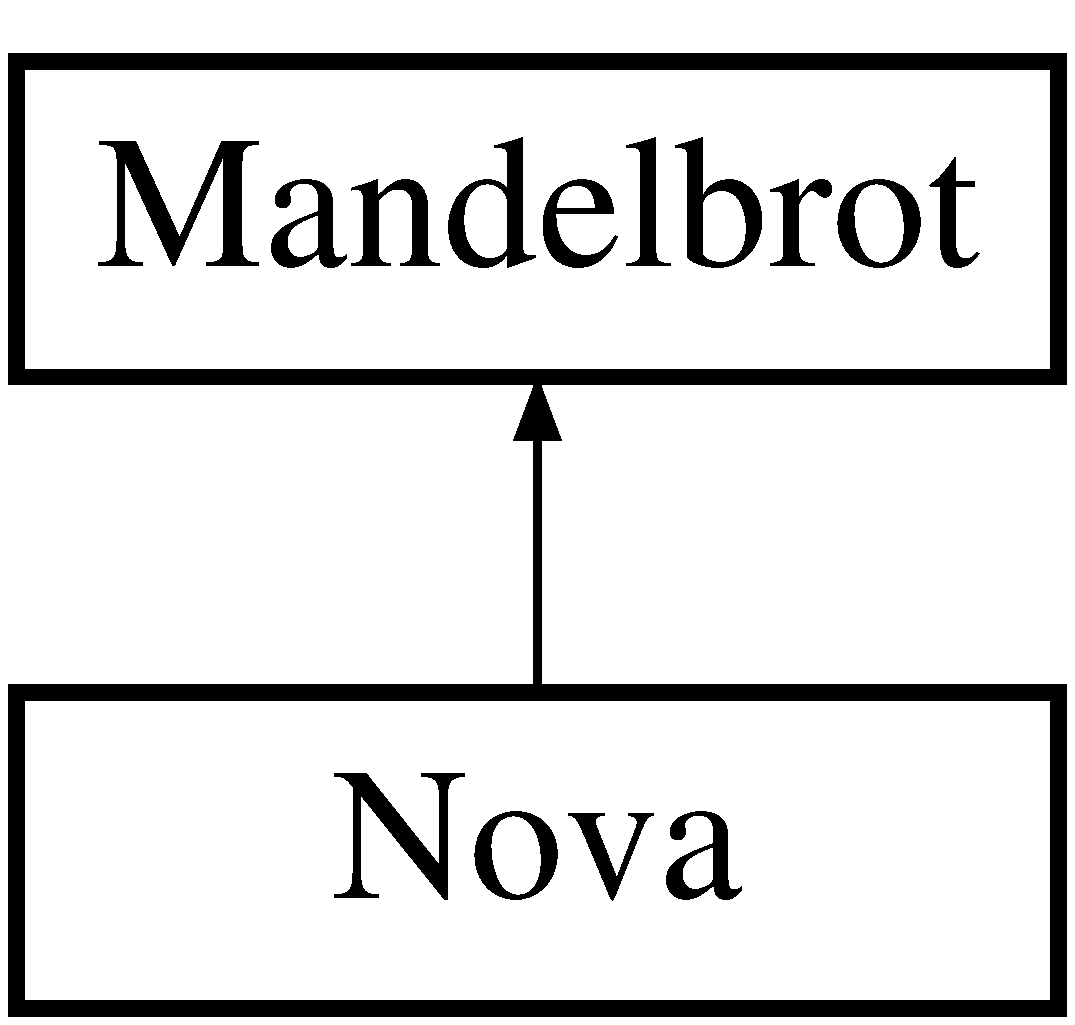
\includegraphics[height=2.000000cm]{class_nova}
\end{center}
\end{figure}
\subsection*{Public Member Functions}
\begin{DoxyCompactItemize}
\item 
\hyperlink{class_nova_a9d171954a6dd98b125587be83ef04db5}{Nova} (unsigned threads, unsigned depth)
\begin{DoxyCompactList}\small\item\em Explicitly constructs a \hyperlink{class_nova}{Nova} set. \end{DoxyCompactList}\item 
void \hyperlink{class_nova_a66935ba0814dfabcae2481c128c336ec}{draw} (\hyperlink{classtsgl_1_1_cartesian_canvas}{Cart} \&can)
\begin{DoxyCompactList}\small\item\em Draw the \hyperlink{class_nova}{Nova} set. \end{DoxyCompactList}\end{DoxyCompactItemize}
\subsection*{Additional Inherited Members}


\subsection{Detailed Description}
Draws a \hyperlink{class_nova}{Nova} (Newton Fractal) set on a Cartesian\+Canvas. 

Extends the \hyperlink{class_mandelbrot}{Mandelbrot} class and overrides its \hyperlink{class_nova_a66935ba0814dfabcae2481c128c336ec}{draw()} function and set\+Redraw() function.

Can zoom in and out of the \hyperlink{class_nova}{Nova} set by scrolling up and down on the mouse wheel (respectively). \begin{DoxySeeAlso}{See also}
\hyperlink{class_mandelbrot}{Mandelbrot} class 
\end{DoxySeeAlso}


\subsection{Constructor \& Destructor Documentation}
\mbox{\Hypertarget{class_nova_a9d171954a6dd98b125587be83ef04db5}\label{class_nova_a9d171954a6dd98b125587be83ef04db5}} 
\index{Nova@{Nova}!Nova@{Nova}}
\index{Nova@{Nova}!Nova@{Nova}}
\subsubsection{\texorpdfstring{Nova()}{Nova()}}
{\footnotesize\ttfamily Nova\+::\+Nova (\begin{DoxyParamCaption}\item[{unsigned}]{threads,  }\item[{unsigned}]{depth }\end{DoxyParamCaption})}



Explicitly constructs a \hyperlink{class_nova}{Nova} set. 

Explicit constructor for the \hyperlink{class_nova}{Nova} class. 
\begin{DoxyParams}{Parameters}
{\em threads} & The number of threads to use in the drawing of the \hyperlink{class_nova}{Nova} object. \\
\hline
{\em depth} & The number of iterations to go to in order to draw the \hyperlink{class_nova}{Nova} object. \\
\hline
\end{DoxyParams}
\begin{DoxyReturn}{Returns}
The \hyperlink{class_nova}{Nova} object ready to be drawn onto the Cartesian\+Canvas. 
\end{DoxyReturn}


\subsection{Member Function Documentation}
\mbox{\Hypertarget{class_nova_a66935ba0814dfabcae2481c128c336ec}\label{class_nova_a66935ba0814dfabcae2481c128c336ec}} 
\index{Nova@{Nova}!draw@{draw}}
\index{draw@{draw}!Nova@{Nova}}
\subsubsection{\texorpdfstring{draw()}{draw()}}
{\footnotesize\ttfamily void Nova\+::draw (\begin{DoxyParamCaption}\item[{\hyperlink{classtsgl_1_1_cartesian_canvas}{Cart} \&}]{can }\end{DoxyParamCaption})\hspace{0.3cm}{\ttfamily [virtual]}}



Draw the \hyperlink{class_nova}{Nova} set. 

Actually draws the \hyperlink{class_nova}{Nova} set onto the Cartesian\+Canvas. 
\begin{DoxyParams}{Parameters}
{\em can} & Reference to the Cartesian\+Canvas to draw to. \\
\hline
\end{DoxyParams}
\begin{DoxyNote}{Note}
This method overrides the \hyperlink{class_mandelbrot}{Mandelbrot} class\textquotesingle{} \hyperlink{class_nova_a66935ba0814dfabcae2481c128c336ec}{draw()} method. 

Cart is a typedef for a Cartesian\+Canvas object. 
\end{DoxyNote}


Reimplemented from \hyperlink{class_mandelbrot_ab7918e4de8f00f73290f110ca7a6cffd}{Mandelbrot}.



The documentation for this class was generated from the following files\+:\begin{DoxyCompactItemize}
\item 
/home/sth5/test/\+T\+S\+G\+L/src/examples/\+Mandelbrot/Nova.\+h\item 
/home/sth5/test/\+T\+S\+G\+L/src/examples/\+Mandelbrot/Nova.\+cpp\end{DoxyCompactItemize}

\hypertarget{class_paddle}{}\section{Paddle Class Reference}
\label{class_paddle}\index{Paddle@{Paddle}}


How can you hit a ball without a paddle?  




{\ttfamily \#include $<$Paddle.\+h$>$}

\subsection*{Public Member Functions}
\begin{DoxyCompactItemize}
\item 
\hyperlink{class_paddle_a5c98ebac2d944073072225b1bb11180a}{Paddle} (\hyperlink{classtsgl_1_1_canvas}{Canvas} \&can, int \&speed, int side)
\begin{DoxyCompactList}\small\item\em Explicitly constructs a \hyperlink{class_paddle}{Paddle} object. \end{DoxyCompactList}\item 
void \hyperlink{class_paddle_ab90901e8e4a4cbf0c99c537583b6ee30}{bindings} (\hyperlink{classtsgl_1_1_canvas}{Canvas} \&can, int side)
\begin{DoxyCompactList}\small\item\em Binds the buttons. \end{DoxyCompactList}\item 
\mbox{\Hypertarget{class_paddle_af18182f0940b764f8e47992f77d3c9dd}\label{class_paddle_af18182f0940b764f8e47992f77d3c9dd}} 
void {\bfseries draw} (\hyperlink{classtsgl_1_1_canvas}{Canvas} \&can, int side)
\item 
\mbox{\Hypertarget{class_paddle_a05d45fe2ca65d7baade4162c56a478f0}\label{class_paddle_a05d45fe2ca65d7baade4162c56a478f0}} 
void \hyperlink{class_paddle_a05d45fe2ca65d7baade4162c56a478f0}{increment} ()
\begin{DoxyCompactList}\small\item\em Increments the \hyperlink{class_paddle}{Paddle} object\textquotesingle{}s score in the game of \hyperlink{class_pong}{Pong}. \end{DoxyCompactList}\item 
\mbox{\Hypertarget{class_paddle_af7552932092d5618b971cd67cefc485f}\label{class_paddle_af7552932092d5618b971cd67cefc485f}} 
void \hyperlink{class_paddle_af7552932092d5618b971cd67cefc485f}{move} ()
\begin{DoxyCompactList}\small\item\em Actually Moves the \hyperlink{class_paddle}{Paddle} object up or down. \end{DoxyCompactList}\item 
int \hyperlink{class_paddle_a4425cbb3e6160de003c7fd364a9ad14b}{get\+Points} () const
\begin{DoxyCompactList}\small\item\em Accessor for the score of the \hyperlink{class_paddle}{Paddle} object. \end{DoxyCompactList}\item 
float \hyperlink{class_paddle_ab27981223156aa4a2b03203733514a6d}{getY} () const
\begin{DoxyCompactList}\small\item\em Accessor for the current y-\/coordinate of the \hyperlink{class_paddle}{Paddle} object. \end{DoxyCompactList}\item 
void \hyperlink{class_paddle_a5f23f811b810d1f4a84b25357bc86e94}{set\+Dir} (int direction)
\begin{DoxyCompactList}\small\item\em Mutator for the direction of the \hyperlink{class_paddle}{Paddle} object. \end{DoxyCompactList}\item 
\mbox{\Hypertarget{class_paddle_ac03c6b92f0b9cd2e67edff4c318ad030}\label{class_paddle_ac03c6b92f0b9cd2e67edff4c318ad030}} 
\hyperlink{class_paddle_ac03c6b92f0b9cd2e67edff4c318ad030}{$\sim$\+Paddle} ()
\begin{DoxyCompactList}\small\item\em Destroys the \hyperlink{class_paddle}{Paddle} object. \end{DoxyCompactList}\end{DoxyCompactItemize}


\subsection{Detailed Description}
How can you hit a ball without a paddle? 

class \hyperlink{class_paddle}{Paddle}

Creates a \hyperlink{class_paddle}{Paddle} in order to play the game, \hyperlink{class_pong}{Pong}.

The W and S keys move the left paddle, the Up and Down arrow keys move the right paddle in the game.

Collisions with the ball are not handled here; they are handled in the \hyperlink{class_pong}{Pong} class\textquotesingle{} draw() method.

The left and right paddles in the game are created from this class; they are essentially the same object. However, there are side parameters in some of the methods that determine which side to place the \hyperlink{class_paddle}{Paddle} object on and how to treat the \hyperlink{class_paddle}{Paddle} object (either as the left or the right paddle in the game). The \hyperlink{class_pong}{Pong} class handles how to distribute points to the \hyperlink{class_paddle}{Paddle} objects in the game (the \hyperlink{class_paddle}{Paddle} class only has an \hyperlink{class_paddle_a05d45fe2ca65d7baade4162c56a478f0}{increment()} method that increments its score counter; the \hyperlink{class_pong}{Pong} class determines which object should call that method when a point is earned). \begin{DoxySeeAlso}{See also}
\hyperlink{class_ball}{Ball} class, \hyperlink{class_pong}{Pong} class. 
\end{DoxySeeAlso}


\subsection{Constructor \& Destructor Documentation}
\mbox{\Hypertarget{class_paddle_a5c98ebac2d944073072225b1bb11180a}\label{class_paddle_a5c98ebac2d944073072225b1bb11180a}} 
\index{Paddle@{Paddle}!Paddle@{Paddle}}
\index{Paddle@{Paddle}!Paddle@{Paddle}}
\subsubsection{\texorpdfstring{Paddle()}{Paddle()}}
{\footnotesize\ttfamily Paddle\+::\+Paddle (\begin{DoxyParamCaption}\item[{\hyperlink{classtsgl_1_1_canvas}{Canvas} \&}]{can,  }\item[{int \&}]{speed,  }\item[{int}]{side }\end{DoxyParamCaption})}



Explicitly constructs a \hyperlink{class_paddle}{Paddle} object. 

Explicit constructor for a \hyperlink{class_paddle}{Paddle} object. 
\begin{DoxyParams}{Parameters}
{\em can} & Reference to the Canvas to have the \hyperlink{class_paddle}{Paddle} object on. \\
\hline
{\em speed} & Reference to the speed of the \hyperlink{class_paddle}{Paddle} object. \\
\hline
\end{DoxyParams}
\begin{DoxyReturn}{Returns}
The constructed \hyperlink{class_paddle}{Paddle} object. 
\end{DoxyReturn}


\subsection{Member Function Documentation}
\mbox{\Hypertarget{class_paddle_ab90901e8e4a4cbf0c99c537583b6ee30}\label{class_paddle_ab90901e8e4a4cbf0c99c537583b6ee30}} 
\index{Paddle@{Paddle}!bindings@{bindings}}
\index{bindings@{bindings}!Paddle@{Paddle}}
\subsubsection{\texorpdfstring{bindings()}{bindings()}}
{\footnotesize\ttfamily void Paddle\+::bindings (\begin{DoxyParamCaption}\item[{\hyperlink{classtsgl_1_1_canvas}{Canvas} \&}]{can,  }\item[{int}]{side }\end{DoxyParamCaption})}



Binds the buttons. 

Binds the buttons with the Canvas. In this case, the keys that move the paddle up and down. 
\begin{DoxyParams}{Parameters}
{\em can} & Reference to the Canvas to bind the keys to. \\
\hline
{\em side} & The side that the \hyperlink{class_paddle}{Paddle} object is on (left = -\/1 and the W and S keys are bound, right = 1 and the Up and Down arrow keys are bound). \\
\hline
\end{DoxyParams}
\mbox{\Hypertarget{class_paddle_a4425cbb3e6160de003c7fd364a9ad14b}\label{class_paddle_a4425cbb3e6160de003c7fd364a9ad14b}} 
\index{Paddle@{Paddle}!get\+Points@{get\+Points}}
\index{get\+Points@{get\+Points}!Paddle@{Paddle}}
\subsubsection{\texorpdfstring{get\+Points()}{getPoints()}}
{\footnotesize\ttfamily int Paddle\+::get\+Points (\begin{DoxyParamCaption}{ }\end{DoxyParamCaption}) const}



Accessor for the score of the \hyperlink{class_paddle}{Paddle} object. 

\begin{DoxyReturn}{Returns}
my\+Points The current score of the \hyperlink{class_paddle}{Paddle} object in the game of \hyperlink{class_pong}{Pong}. 
\end{DoxyReturn}
\mbox{\Hypertarget{class_paddle_ab27981223156aa4a2b03203733514a6d}\label{class_paddle_ab27981223156aa4a2b03203733514a6d}} 
\index{Paddle@{Paddle}!getY@{getY}}
\index{getY@{getY}!Paddle@{Paddle}}
\subsubsection{\texorpdfstring{get\+Y()}{getY()}}
{\footnotesize\ttfamily float Paddle\+::getY (\begin{DoxyParamCaption}{ }\end{DoxyParamCaption}) const}



Accessor for the current y-\/coordinate of the \hyperlink{class_paddle}{Paddle} object. 

\begin{DoxyReturn}{Returns}
myY The y-\/coordinate of the \hyperlink{class_paddle}{Paddle} object. 
\end{DoxyReturn}
\mbox{\Hypertarget{class_paddle_a5f23f811b810d1f4a84b25357bc86e94}\label{class_paddle_a5f23f811b810d1f4a84b25357bc86e94}} 
\index{Paddle@{Paddle}!set\+Dir@{set\+Dir}}
\index{set\+Dir@{set\+Dir}!Paddle@{Paddle}}
\subsubsection{\texorpdfstring{set\+Dir()}{setDir()}}
{\footnotesize\ttfamily void Paddle\+::set\+Dir (\begin{DoxyParamCaption}\item[{int}]{direction }\end{DoxyParamCaption})}



Mutator for the direction of the \hyperlink{class_paddle}{Paddle} object. 

Changes the current direction of the \hyperlink{class_paddle}{Paddle} object (up or down). 

The documentation for this class was generated from the following files\+:\begin{DoxyCompactItemize}
\item 
/home/sth5/test/\+T\+S\+G\+L/src/examples/\+Pong/Paddle.\+h\item 
/home/sth5/test/\+T\+S\+G\+L/src/examples/\+Pong/Paddle.\+cpp\end{DoxyCompactItemize}

\hypertarget{class_p_c_thread}{}\section{P\+C\+Thread Class Reference}
\label{class_p_c_thread}\index{P\+C\+Thread@{P\+C\+Thread}}


{\ttfamily \#include $<$P\+C\+Thread.\+h$>$}

Inheritance diagram for P\+C\+Thread\+:\begin{figure}[H]
\begin{center}
\leavevmode
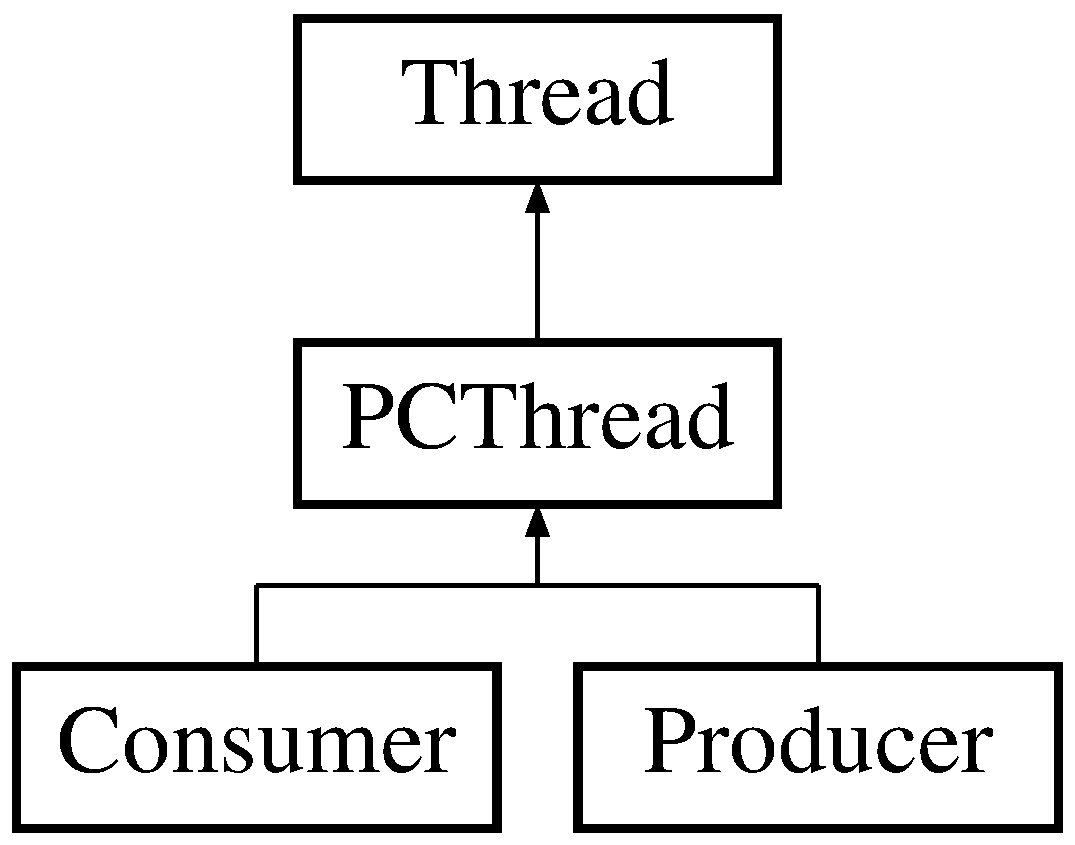
\includegraphics[height=3.000000cm]{class_p_c_thread}
\end{center}
\end{figure}
\subsection*{Public Member Functions}
\begin{DoxyCompactItemize}
\item 
\hyperlink{class_p_c_thread_a7ae0244c033e4202d2643544432f91f7}{P\+C\+Thread} ()
\begin{DoxyCompactList}\small\item\em Default-\/constructor for the \hyperlink{class_p_c_thread}{P\+C\+Thread} class. \end{DoxyCompactList}\item 
\hyperlink{class_p_c_thread_abe06615f59879c19d703a93889f5e7cc}{P\+C\+Thread} (\hyperlink{class_queue}{Queue}$<$ \hyperlink{classtsgl_1_1_star}{Star} $\ast$$>$ \&shared\+Buffer, unsigned long id, \hyperlink{classtsgl_1_1_canvas}{Canvas} \&can)
\item 
\mbox{\Hypertarget{class_p_c_thread_a57df324beabfba54ebee6a7c59bf49ef}\label{class_p_c_thread_a57df324beabfba54ebee6a7c59bf49ef}} 
virtual void {\bfseries run} ()
\item 
\mbox{\Hypertarget{class_p_c_thread_a7ca73de5a86008e76797ad134bca5f33}\label{class_p_c_thread_a7ca73de5a86008e76797ad134bca5f33}} 
virtual void {\bfseries wait} ()
\item 
\mbox{\Hypertarget{class_p_c_thread_a7a8bb7e11ecc298ae012f4393902c58c}\label{class_p_c_thread_a7a8bb7e11ecc298ae012f4393902c58c}} 
virtual void {\bfseries lock} ()=0
\item 
\mbox{\Hypertarget{class_p_c_thread_ada80e2193c24b9111eb21abd07b2e2a1}\label{class_p_c_thread_ada80e2193c24b9111eb21abd07b2e2a1}} 
virtual void {\bfseries act} ()=0
\item 
\mbox{\Hypertarget{class_p_c_thread_a6266054bfef3bae0fceeefe00f64cc17}\label{class_p_c_thread_a6266054bfef3bae0fceeefe00f64cc17}} 
virtual void {\bfseries unlock} ()=0
\end{DoxyCompactItemize}
\subsection*{Static Public Attributes}
\begin{DoxyCompactItemize}
\item 
\mbox{\Hypertarget{class_p_c_thread_acee1e97e483e422b8845704f1fa3f793}\label{class_p_c_thread_acee1e97e483e422b8845704f1fa3f793}} 
static std\+::atomic$<$ bool $>$ {\bfseries paused}
\end{DoxyCompactItemize}
\subsection*{Protected Member Functions}
\begin{DoxyCompactItemize}
\item 
\mbox{\Hypertarget{class_p_c_thread_a82130f5a7e30132226be3f9966b1e526}\label{class_p_c_thread_a82130f5a7e30132226be3f9966b1e526}} 
void {\bfseries animate\+Item} (int endX, int endY)
\end{DoxyCompactItemize}
\subsection*{Protected Attributes}
\begin{DoxyCompactItemize}
\item 
\mbox{\Hypertarget{class_p_c_thread_ae2b90159f35617ed516678314db7e7bd}\label{class_p_c_thread_ae2b90159f35617ed516678314db7e7bd}} 
int {\bfseries myX}
\item 
\mbox{\Hypertarget{class_p_c_thread_a604e02565566f31468557ca79a610164}\label{class_p_c_thread_a604e02565566f31468557ca79a610164}} 
int {\bfseries myY}
\item 
\mbox{\Hypertarget{class_p_c_thread_a8107e048d3340e5cb40af9ed613f4c20}\label{class_p_c_thread_a8107e048d3340e5cb40af9ed613f4c20}} 
int {\bfseries count}
\item 
\mbox{\Hypertarget{class_p_c_thread_aeabf35c11ce3b710a8a77a1f8668a566}\label{class_p_c_thread_aeabf35c11ce3b710a8a77a1f8668a566}} 
\hyperlink{class_queue}{Queue}$<$ \hyperlink{classtsgl_1_1_star}{Star} $\ast$ $>$ $\ast$ {\bfseries buffer}
\item 
\mbox{\Hypertarget{class_p_c_thread_af9e9d19ab5bf1270941196546953a8f1}\label{class_p_c_thread_af9e9d19ab5bf1270941196546953a8f1}} 
\hyperlink{classtsgl_1_1_canvas}{Canvas} $\ast$ {\bfseries my\+Can}
\item 
\mbox{\Hypertarget{class_p_c_thread_add7f6d91944182daddcc3046fe3888dc}\label{class_p_c_thread_add7f6d91944182daddcc3046fe3888dc}} 
\hyperlink{classtsgl_1_1_convex_polygon}{Convex\+Polygon} $\ast$ {\bfseries my\+Shape}
\item 
\mbox{\Hypertarget{class_p_c_thread_a07bd5b9a44cd4cf624926cb98ee31be2}\label{class_p_c_thread_a07bd5b9a44cd4cf624926cb98ee31be2}} 
\hyperlink{classtsgl_1_1_arrow}{Arrow} $\ast$ {\bfseries my\+Arrow}
\item 
\mbox{\Hypertarget{class_p_c_thread_a3ca420c0690790d3c3fbd2e180f0ce15}\label{class_p_c_thread_a3ca420c0690790d3c3fbd2e180f0ce15}} 
\hyperlink{classtsgl_1_1_star}{Star} $\ast$ {\bfseries my\+Item}
\item 
\mbox{\Hypertarget{class_p_c_thread_a2b37315ff24869556be743aea49def26}\label{class_p_c_thread_a2b37315ff24869556be743aea49def26}} 
\hyperlink{classtsgl_1_1_text}{Text} $\ast$ {\bfseries my\+Count\+Label}
\end{DoxyCompactItemize}
\subsection*{Additional Inherited Members}


\subsection{Detailed Description}
P\+Chread class inherits from the \hyperlink{class_thread}{Thread} class in order to create a \hyperlink{class_p_c_thread}{P\+C\+Thread} object. Inheritance\+: \hyperlink{class_thread}{Thread} class. 

\subsection{Constructor \& Destructor Documentation}
\mbox{\Hypertarget{class_p_c_thread_a7ae0244c033e4202d2643544432f91f7}\label{class_p_c_thread_a7ae0244c033e4202d2643544432f91f7}} 
\index{P\+C\+Thread@{P\+C\+Thread}!P\+C\+Thread@{P\+C\+Thread}}
\index{P\+C\+Thread@{P\+C\+Thread}!P\+C\+Thread@{P\+C\+Thread}}
\subsubsection{\texorpdfstring{P\+C\+Thread()}{PCThread()}\hspace{0.1cm}{\footnotesize\ttfamily [1/2]}}
{\footnotesize\ttfamily P\+C\+Thread\+::\+P\+C\+Thread (\begin{DoxyParamCaption}{ }\end{DoxyParamCaption})}



Default-\/constructor for the \hyperlink{class_p_c_thread}{P\+C\+Thread} class. 

\begin{DoxyReturn}{Returns}
\+: The constructed \hyperlink{class_p_c_thread}{P\+C\+Thread} object. 
\end{DoxyReturn}
\mbox{\Hypertarget{class_p_c_thread_abe06615f59879c19d703a93889f5e7cc}\label{class_p_c_thread_abe06615f59879c19d703a93889f5e7cc}} 
\index{P\+C\+Thread@{P\+C\+Thread}!P\+C\+Thread@{P\+C\+Thread}}
\index{P\+C\+Thread@{P\+C\+Thread}!P\+C\+Thread@{P\+C\+Thread}}
\subsubsection{\texorpdfstring{P\+C\+Thread()}{PCThread()}\hspace{0.1cm}{\footnotesize\ttfamily [2/2]}}
{\footnotesize\ttfamily P\+C\+Thread\+::\+P\+C\+Thread (\begin{DoxyParamCaption}\item[{\hyperlink{class_queue}{Queue}$<$ \hyperlink{classtsgl_1_1_star}{Star} $\ast$$>$ \&}]{shared\+Buffer,  }\item[{unsigned long}]{id,  }\item[{\hyperlink{classtsgl_1_1_canvas}{Canvas} \&}]{can }\end{DoxyParamCaption})}

Explicit-\/constructor for the \hyperlink{class_p_c_thread}{P\+C\+Thread} class. param\+: shared\+Buffer, a reference to the \hyperlink{class_queue}{Queue} object that is shared between the \hyperlink{class_producer}{Producer} and \hyperlink{class_consumer}{Consumer}. param\+: id, an unsigned long that will be passed to the \hyperlink{class_thread_a95c703fb8f2f27cb64f475a8c940864a}{Thread()} constructor that will act as the id for the \hyperlink{class_thread}{Thread} object. param\+: can, a handle to the Canvas that will be drawn on and will determine whether or not to continue consuming objects from the \hyperlink{class_queue}{Queue}. return\+: The constructed \hyperlink{class_p_c_thread}{P\+C\+Thread} object. 

The documentation for this class was generated from the following files\+:\begin{DoxyCompactItemize}
\item 
/home/sth5/test/\+T\+S\+G\+L/src/examples/\+Producer\+Consumer/P\+C\+Thread.\+h\item 
/home/sth5/test/\+T\+S\+G\+L/src/examples/\+Producer\+Consumer/P\+C\+Thread.\+cpp\end{DoxyCompactItemize}

\hypertarget{class_philosopher}{}\section{Philosopher Class Reference}
\label{class_philosopher}\index{Philosopher@{Philosopher}}


Object representing a philosopher in the Dining Philosophers\textquotesingle{} problem.  




{\ttfamily \#include $<$Philosopher.\+h$>$}

\subsection*{Public Member Functions}
\begin{DoxyCompactItemize}
\item 
\hyperlink{class_philosopher_affffff67acd52b945fb91277c52af8a3}{Philosopher} ()
\begin{DoxyCompactList}\small\item\em Explicitly constructs a new \hyperlink{class_philosopher}{Philosopher}. \end{DoxyCompactList}\item 
void \hyperlink{class_philosopher_a0b49a5a22cd608ce3ac73211df0d3f45}{draw} (\hyperlink{classtsgl_1_1_canvas}{Canvas} \&can, float x, float y)
\item 
void \hyperlink{class_philosopher_ae0d341934c25f1303ea0c16228e9eeae}{refresh\+Color} ()
\item 
void \hyperlink{class_philosopher_a5e5cfa25abdbca70a5d9ae725d8df7ea}{add\+Meal} ()
\item 
bool \hyperlink{class_philosopher_a7658c8e95d7895246251b494b033d2e3}{acquire} (\hyperlink{struct_fork}{Fork} \&f)
\item 
bool \hyperlink{class_philosopher_a0d229ee7b31b4ccd530fced5424f84a9}{release} (\hyperlink{struct_fork}{Fork} \&f)
\item 
void \hyperlink{class_philosopher_adb8c98df2b7cf8f2d2cde2daa18c731a}{think} ()
\item 
\mbox{\Hypertarget{class_philosopher_a0115c91983e00c09663f36a7b275e1bd}\label{class_philosopher_a0115c91983e00c09663f36a7b275e1bd}} 
void \hyperlink{class_philosopher_a0115c91983e00c09663f36a7b275e1bd}{eat} ()
\begin{DoxyCompactList}\small\item\em Resets the \hyperlink{class_philosopher}{Philosopher} to thinking after he eats. \end{DoxyCompactList}\item 
void \hyperlink{class_philosopher_ad17179822ef90cea812252fa11709ad7}{set\+State} (Phil\+State s)
\begin{DoxyCompactList}\small\item\em Mutator for my\+State. \end{DoxyCompactList}\item 
void \hyperlink{class_philosopher_afbeb831cc699beac308607e43ca0693d}{set\+Action} (Phil\+Action a)
\begin{DoxyCompactList}\small\item\em Mutator for my\+Action. \end{DoxyCompactList}\item 
void \hyperlink{class_philosopher_a052dca3c30eb699b594aa0c086554a30}{set\+Id} (int i, int nphil)
\begin{DoxyCompactList}\small\item\em Mutator for id. \end{DoxyCompactList}\item 
int \hyperlink{class_philosopher_aec2c6ca7096a9ae51f35e0f68b167345}{get\+Meals} ()
\item 
Phil\+State \hyperlink{class_philosopher_a04862832ab8b79fd45ddec5e0546775a}{state} ()
\item 
Phil\+Action \hyperlink{class_philosopher_a0e6078cacfe93f71cc7f027e0b3a8971}{action} ()
\item 
int \hyperlink{class_philosopher_adea5fd87303d0365985cb87c7666e452}{get\+Id} ()
\item 
bool \hyperlink{class_philosopher_a3718addd7037cd1266435e7c91e84388}{has\+Circle} ()
\end{DoxyCompactItemize}


\subsection{Detailed Description}
Object representing a philosopher in the Dining Philosophers\textquotesingle{} problem. 

The \hyperlink{class_philosopher}{Philosopher} class contains variables and methods necessary for representing a philosopher at a table. Each \hyperlink{class_philosopher}{Philosopher} may acquire or release the fork to his left or to his right (or both), with his state changing accordingly. 

\subsection{Constructor \& Destructor Documentation}
\mbox{\Hypertarget{class_philosopher_affffff67acd52b945fb91277c52af8a3}\label{class_philosopher_affffff67acd52b945fb91277c52af8a3}} 
\index{Philosopher@{Philosopher}!Philosopher@{Philosopher}}
\index{Philosopher@{Philosopher}!Philosopher@{Philosopher}}
\subsubsection{\texorpdfstring{Philosopher()}{Philosopher()}}
{\footnotesize\ttfamily Philosopher\+::\+Philosopher (\begin{DoxyParamCaption}{ }\end{DoxyParamCaption})}



Explicitly constructs a new \hyperlink{class_philosopher}{Philosopher}. 

Explicit constructor for a new \hyperlink{class_philosopher}{Philosopher} object. 

\subsection{Member Function Documentation}
\mbox{\Hypertarget{class_philosopher_a7658c8e95d7895246251b494b033d2e3}\label{class_philosopher_a7658c8e95d7895246251b494b033d2e3}} 
\index{Philosopher@{Philosopher}!acquire@{acquire}}
\index{acquire@{acquire}!Philosopher@{Philosopher}}
\subsubsection{\texorpdfstring{acquire()}{acquire()}}
{\footnotesize\ttfamily bool Philosopher\+::acquire (\begin{DoxyParamCaption}\item[{\hyperlink{struct_fork}{Fork} \&}]{f }\end{DoxyParamCaption})}

Picks up a fork specified by its reference 

Referenced by Table\+::act\+Step().

\mbox{\Hypertarget{class_philosopher_a0e6078cacfe93f71cc7f027e0b3a8971}\label{class_philosopher_a0e6078cacfe93f71cc7f027e0b3a8971}} 
\index{Philosopher@{Philosopher}!action@{action}}
\index{action@{action}!Philosopher@{Philosopher}}
\subsubsection{\texorpdfstring{action()}{action()}}
{\footnotesize\ttfamily Phil\+Action Philosopher\+::action (\begin{DoxyParamCaption}{ }\end{DoxyParamCaption})\hspace{0.3cm}{\ttfamily [inline]}}

Accessor for \hyperlink{class_philosopher}{Philosopher}\textquotesingle{}s action. \mbox{\Hypertarget{class_philosopher_a5e5cfa25abdbca70a5d9ae725d8df7ea}\label{class_philosopher_a5e5cfa25abdbca70a5d9ae725d8df7ea}} 
\index{Philosopher@{Philosopher}!add\+Meal@{add\+Meal}}
\index{add\+Meal@{add\+Meal}!Philosopher@{Philosopher}}
\subsubsection{\texorpdfstring{add\+Meal()}{addMeal()}}
{\footnotesize\ttfamily void Philosopher\+::add\+Meal (\begin{DoxyParamCaption}{ }\end{DoxyParamCaption})}

Adds a meal representation to meals and the Canvas 

Referenced by Table\+::draw\+Step().

\mbox{\Hypertarget{class_philosopher_a0b49a5a22cd608ce3ac73211df0d3f45}\label{class_philosopher_a0b49a5a22cd608ce3ac73211df0d3f45}} 
\index{Philosopher@{Philosopher}!draw@{draw}}
\index{draw@{draw}!Philosopher@{Philosopher}}
\subsubsection{\texorpdfstring{draw()}{draw()}}
{\footnotesize\ttfamily void Philosopher\+::draw (\begin{DoxyParamCaption}\item[{\hyperlink{classtsgl_1_1_canvas}{Canvas} \&}]{can,  }\item[{float}]{x,  }\item[{float}]{y }\end{DoxyParamCaption})}

Adds \hyperlink{class_philosopher}{Philosopher} to Canvas or refreshes its color. 

Referenced by Table\+::draw\+Step().

\mbox{\Hypertarget{class_philosopher_adea5fd87303d0365985cb87c7666e452}\label{class_philosopher_adea5fd87303d0365985cb87c7666e452}} 
\index{Philosopher@{Philosopher}!get\+Id@{get\+Id}}
\index{get\+Id@{get\+Id}!Philosopher@{Philosopher}}
\subsubsection{\texorpdfstring{get\+Id()}{getId()}}
{\footnotesize\ttfamily int Philosopher\+::get\+Id (\begin{DoxyParamCaption}{ }\end{DoxyParamCaption})\hspace{0.3cm}{\ttfamily [inline]}}

Accessor for \hyperlink{class_philosopher}{Philosopher}\textquotesingle{}s id. \mbox{\Hypertarget{class_philosopher_aec2c6ca7096a9ae51f35e0f68b167345}\label{class_philosopher_aec2c6ca7096a9ae51f35e0f68b167345}} 
\index{Philosopher@{Philosopher}!get\+Meals@{get\+Meals}}
\index{get\+Meals@{get\+Meals}!Philosopher@{Philosopher}}
\subsubsection{\texorpdfstring{get\+Meals()}{getMeals()}}
{\footnotesize\ttfamily int Philosopher\+::get\+Meals (\begin{DoxyParamCaption}{ }\end{DoxyParamCaption})\hspace{0.3cm}{\ttfamily [inline]}}

Accessor for number of meals \hyperlink{class_philosopher}{Philosopher} has consumed. 

Referenced by Table\+::draw\+Step().

\mbox{\Hypertarget{class_philosopher_a3718addd7037cd1266435e7c91e84388}\label{class_philosopher_a3718addd7037cd1266435e7c91e84388}} 
\index{Philosopher@{Philosopher}!has\+Circle@{has\+Circle}}
\index{has\+Circle@{has\+Circle}!Philosopher@{Philosopher}}
\subsubsection{\texorpdfstring{has\+Circle()}{hasCircle()}}
{\footnotesize\ttfamily bool Philosopher\+::has\+Circle (\begin{DoxyParamCaption}{ }\end{DoxyParamCaption})\hspace{0.3cm}{\ttfamily [inline]}}

Accessor for \hyperlink{class_philosopher}{Philosopher}\textquotesingle{}s circle. \mbox{\Hypertarget{class_philosopher_ae0d341934c25f1303ea0c16228e9eeae}\label{class_philosopher_ae0d341934c25f1303ea0c16228e9eeae}} 
\index{Philosopher@{Philosopher}!refresh\+Color@{refresh\+Color}}
\index{refresh\+Color@{refresh\+Color}!Philosopher@{Philosopher}}
\subsubsection{\texorpdfstring{refresh\+Color()}{refreshColor()}}
{\footnotesize\ttfamily void Philosopher\+::refresh\+Color (\begin{DoxyParamCaption}{ }\end{DoxyParamCaption})}

Updates the \hyperlink{class_philosopher}{Philosopher}\textquotesingle{}s color based on its state 

Referenced by Table\+::draw\+Step().

\mbox{\Hypertarget{class_philosopher_a0d229ee7b31b4ccd530fced5424f84a9}\label{class_philosopher_a0d229ee7b31b4ccd530fced5424f84a9}} 
\index{Philosopher@{Philosopher}!release@{release}}
\index{release@{release}!Philosopher@{Philosopher}}
\subsubsection{\texorpdfstring{release()}{release()}}
{\footnotesize\ttfamily bool Philosopher\+::release (\begin{DoxyParamCaption}\item[{\hyperlink{struct_fork}{Fork} \&}]{f }\end{DoxyParamCaption})}

Releases a fork specified by its reference 

Referenced by Table\+::act\+Step().

\mbox{\Hypertarget{class_philosopher_afbeb831cc699beac308607e43ca0693d}\label{class_philosopher_afbeb831cc699beac308607e43ca0693d}} 
\index{Philosopher@{Philosopher}!set\+Action@{set\+Action}}
\index{set\+Action@{set\+Action}!Philosopher@{Philosopher}}
\subsubsection{\texorpdfstring{set\+Action()}{setAction()}}
{\footnotesize\ttfamily void Philosopher\+::set\+Action (\begin{DoxyParamCaption}\item[{Phil\+Action}]{a }\end{DoxyParamCaption})\hspace{0.3cm}{\ttfamily [inline]}}



Mutator for my\+Action. 


\begin{DoxyParams}{Parameters}
{\em s} & Phil\+Action to set my\+Action to. \\
\hline
\end{DoxyParams}


Referenced by Table\+::forfeit\+When\+Blocked\+Method(), Table\+::hierarchy\+Method(), Table\+::n\+Frame\+Release\+Method(), Table\+::odd\+Even\+Method(), think(), and Table\+::wait\+When\+Blocked\+Method().

\mbox{\Hypertarget{class_philosopher_a052dca3c30eb699b594aa0c086554a30}\label{class_philosopher_a052dca3c30eb699b594aa0c086554a30}} 
\index{Philosopher@{Philosopher}!set\+Id@{set\+Id}}
\index{set\+Id@{set\+Id}!Philosopher@{Philosopher}}
\subsubsection{\texorpdfstring{set\+Id()}{setId()}}
{\footnotesize\ttfamily void Philosopher\+::set\+Id (\begin{DoxyParamCaption}\item[{int}]{i,  }\item[{int}]{nphil }\end{DoxyParamCaption})\hspace{0.3cm}{\ttfamily [inline]}}



Mutator for id. 


\begin{DoxyParams}{Parameters}
{\em i} & Which philosopher id to mutate \\
\hline
{\em nphil} & Total number of philosophers. \\
\hline
\end{DoxyParams}


Referenced by Philosopher(), and Table\+::\+Table().

\mbox{\Hypertarget{class_philosopher_ad17179822ef90cea812252fa11709ad7}\label{class_philosopher_ad17179822ef90cea812252fa11709ad7}} 
\index{Philosopher@{Philosopher}!set\+State@{set\+State}}
\index{set\+State@{set\+State}!Philosopher@{Philosopher}}
\subsubsection{\texorpdfstring{set\+State()}{setState()}}
{\footnotesize\ttfamily void Philosopher\+::set\+State (\begin{DoxyParamCaption}\item[{Phil\+State}]{s }\end{DoxyParamCaption})\hspace{0.3cm}{\ttfamily [inline]}}



Mutator for my\+State. 


\begin{DoxyParams}{Parameters}
{\em s} & Phil\+State to set my\+State to. \\
\hline
\end{DoxyParams}


Referenced by Table\+::forfeit\+When\+Blocked\+Method(), and think().

\mbox{\Hypertarget{class_philosopher_a04862832ab8b79fd45ddec5e0546775a}\label{class_philosopher_a04862832ab8b79fd45ddec5e0546775a}} 
\index{Philosopher@{Philosopher}!state@{state}}
\index{state@{state}!Philosopher@{Philosopher}}
\subsubsection{\texorpdfstring{state()}{state()}}
{\footnotesize\ttfamily Phil\+State Philosopher\+::state (\begin{DoxyParamCaption}{ }\end{DoxyParamCaption})\hspace{0.3cm}{\ttfamily [inline]}}

Accessor for \hyperlink{class_philosopher}{Philosopher}\textquotesingle{}s state. 

Referenced by Table\+::draw\+Step().

\mbox{\Hypertarget{class_philosopher_adb8c98df2b7cf8f2d2cde2daa18c731a}\label{class_philosopher_adb8c98df2b7cf8f2d2cde2daa18c731a}} 
\index{Philosopher@{Philosopher}!think@{think}}
\index{think@{think}!Philosopher@{Philosopher}}
\subsubsection{\texorpdfstring{think()}{think()}}
{\footnotesize\ttfamily void Philosopher\+::think (\begin{DoxyParamCaption}{ }\end{DoxyParamCaption})}

Thinks and switches to hungry state if a random number is a multiple of 3. 

Referenced by Table\+::hierarchy\+Method(), Table\+::n\+Frame\+Release\+Method(), Table\+::odd\+Even\+Method(), and Table\+::wait\+When\+Blocked\+Method().



The documentation for this class was generated from the following files\+:\begin{DoxyCompactItemize}
\item 
/home/sth5/test/\+T\+S\+G\+L/src/examples/\+Dining\+Philosophers/Philosopher.\+h\item 
/home/sth5/test/\+T\+S\+G\+L/src/examples/\+Dining\+Philosophers/Philosopher.\+cpp\end{DoxyCompactItemize}

\hypertarget{class_philosopher3_d}{}\section{Philosopher3D Class Reference}
\label{class_philosopher3_d}\index{Philosopher3D@{Philosopher3D}}


Object representing a 3D philosopher in the Dining Philosophers\textquotesingle{} problem.  




{\ttfamily \#include $<$Philosopher3\+D.\+h$>$}

\subsection*{Public Member Functions}
\begin{DoxyCompactItemize}
\item 
\hyperlink{class_philosopher3_d_ac45678c5f33b97bcff814df559ea0ebb}{Philosopher3D} ()
\begin{DoxyCompactList}\small\item\em Explicitly constructs a new \hyperlink{class_philosopher3_d}{Philosopher3D}. \end{DoxyCompactList}\item 
void \hyperlink{class_philosopher3_d_af9321231d363ade9c90bf381650bebb7}{draw} (\hyperlink{classtsgl_1_1_canvas}{Canvas} \&can, float x, float y)
\item 
void \hyperlink{class_philosopher3_d_abadf81910034cbd6757d6fac2d1154a5}{refresh\+Color} ()
\item 
void \hyperlink{class_philosopher3_d_a536c633359c82402055c6264cc8f12cc}{add\+Meal} (float x, float y, float z)
\item 
\mbox{\Hypertarget{class_philosopher3_d_aecd0b8eba2c5f672f4823b46759fd9d2}\label{class_philosopher3_d_aecd0b8eba2c5f672f4823b46759fd9d2}} 
\hyperlink{classtsgl_1_1_pyramid}{Pyramid} $\ast$ {\bfseries get\+Last\+Meal} ()
\item 
bool \hyperlink{class_philosopher3_d_a55a0b5fa883f9304e93e386d75b0cb2a}{acquire} (\hyperlink{struct_fork3_d}{Fork3D} \&f)
\item 
bool \hyperlink{class_philosopher3_d_ab6fcdb12fb04651f33005c891f89791e}{release} (\hyperlink{struct_fork3_d}{Fork3D} \&f)
\item 
void \hyperlink{class_philosopher3_d_a586456ca9cc859018aa47564f235c933}{think} ()
\item 
\mbox{\Hypertarget{class_philosopher3_d_a0fd066c61fec3adfdcd80eea1793fba7}\label{class_philosopher3_d_a0fd066c61fec3adfdcd80eea1793fba7}} 
void \hyperlink{class_philosopher3_d_a0fd066c61fec3adfdcd80eea1793fba7}{eat} ()
\begin{DoxyCompactList}\small\item\em Resets the \hyperlink{class_philosopher3_d}{Philosopher3D} to thinking after he eats. \end{DoxyCompactList}\item 
void \hyperlink{class_philosopher3_d_ad9c54065af476b716f985c0ae3d4bd21}{set\+State} (Phil\+State s)
\begin{DoxyCompactList}\small\item\em Mutator for my\+State. \end{DoxyCompactList}\item 
void \hyperlink{class_philosopher3_d_ab261853f450bfb3bcd25eb397893dba2}{set\+Action} (Phil\+Action a)
\begin{DoxyCompactList}\small\item\em Mutator for my\+Action. \end{DoxyCompactList}\item 
void \hyperlink{class_philosopher3_d_a748b557b785461ca3e1b3d44e658f9af}{set\+Id} (int i, int nphil)
\begin{DoxyCompactList}\small\item\em Mutator for id. \end{DoxyCompactList}\item 
int \hyperlink{class_philosopher3_d_a7bff098afeb987e4fe4fab2dd6adcad6}{get\+Meals} ()
\item 
Phil\+State \hyperlink{class_philosopher3_d_a515fb48855cd2a9421c13d6097953a10}{state} ()
\item 
Phil\+Action \hyperlink{class_philosopher3_d_a4dc5329e128f072695d216af3867b4b4}{action} ()
\item 
int \hyperlink{class_philosopher3_d_aa1b77e0ee22ef9eb661cbc83b90d163b}{get\+Id} ()
\item 
bool \hyperlink{class_philosopher3_d_a85edb411abaa49e0cc6fb8f8791bdb8b}{has\+Cylinder} ()
\end{DoxyCompactItemize}


\subsection{Detailed Description}
Object representing a 3D philosopher in the Dining Philosophers\textquotesingle{} problem. 

The \hyperlink{class_philosopher3_d}{Philosopher3D} class contains variables and methods necessary for representing a philosopher at a table. Each \hyperlink{class_philosopher3_d}{Philosopher3D} may acquire or release the fork to his left or to his right (or both), with his state changing accordingly. 

\subsection{Constructor \& Destructor Documentation}
\mbox{\Hypertarget{class_philosopher3_d_ac45678c5f33b97bcff814df559ea0ebb}\label{class_philosopher3_d_ac45678c5f33b97bcff814df559ea0ebb}} 
\index{Philosopher3D@{Philosopher3D}!Philosopher3D@{Philosopher3D}}
\index{Philosopher3D@{Philosopher3D}!Philosopher3D@{Philosopher3D}}
\subsubsection{\texorpdfstring{Philosopher3\+D()}{Philosopher3D()}}
{\footnotesize\ttfamily Philosopher3\+D\+::\+Philosopher3D (\begin{DoxyParamCaption}{ }\end{DoxyParamCaption})}



Explicitly constructs a new \hyperlink{class_philosopher3_d}{Philosopher3D}. 

Explicit constructor for a new \hyperlink{class_philosopher3_d}{Philosopher3D} object. 

\subsection{Member Function Documentation}
\mbox{\Hypertarget{class_philosopher3_d_a55a0b5fa883f9304e93e386d75b0cb2a}\label{class_philosopher3_d_a55a0b5fa883f9304e93e386d75b0cb2a}} 
\index{Philosopher3D@{Philosopher3D}!acquire@{acquire}}
\index{acquire@{acquire}!Philosopher3D@{Philosopher3D}}
\subsubsection{\texorpdfstring{acquire()}{acquire()}}
{\footnotesize\ttfamily bool Philosopher3\+D\+::acquire (\begin{DoxyParamCaption}\item[{\hyperlink{struct_fork3_d}{Fork3D} \&}]{f }\end{DoxyParamCaption})}

Picks up a fork specified by its reference 

Referenced by Table3\+D\+::act\+Step().

\mbox{\Hypertarget{class_philosopher3_d_a4dc5329e128f072695d216af3867b4b4}\label{class_philosopher3_d_a4dc5329e128f072695d216af3867b4b4}} 
\index{Philosopher3D@{Philosopher3D}!action@{action}}
\index{action@{action}!Philosopher3D@{Philosopher3D}}
\subsubsection{\texorpdfstring{action()}{action()}}
{\footnotesize\ttfamily Phil\+Action Philosopher3\+D\+::action (\begin{DoxyParamCaption}{ }\end{DoxyParamCaption})\hspace{0.3cm}{\ttfamily [inline]}}

Accessor for \hyperlink{class_philosopher3_d}{Philosopher3D}\textquotesingle{}s action. \mbox{\Hypertarget{class_philosopher3_d_a536c633359c82402055c6264cc8f12cc}\label{class_philosopher3_d_a536c633359c82402055c6264cc8f12cc}} 
\index{Philosopher3D@{Philosopher3D}!add\+Meal@{add\+Meal}}
\index{add\+Meal@{add\+Meal}!Philosopher3D@{Philosopher3D}}
\subsubsection{\texorpdfstring{add\+Meal()}{addMeal()}}
{\footnotesize\ttfamily void Philosopher3\+D\+::add\+Meal (\begin{DoxyParamCaption}\item[{float}]{x,  }\item[{float}]{y,  }\item[{float}]{z }\end{DoxyParamCaption})}

Adds a meal representation to meals and the Canvas 

Referenced by Table3\+D\+::draw\+Step().

\mbox{\Hypertarget{class_philosopher3_d_af9321231d363ade9c90bf381650bebb7}\label{class_philosopher3_d_af9321231d363ade9c90bf381650bebb7}} 
\index{Philosopher3D@{Philosopher3D}!draw@{draw}}
\index{draw@{draw}!Philosopher3D@{Philosopher3D}}
\subsubsection{\texorpdfstring{draw()}{draw()}}
{\footnotesize\ttfamily void Philosopher3\+D\+::draw (\begin{DoxyParamCaption}\item[{\hyperlink{classtsgl_1_1_canvas}{Canvas} \&}]{can,  }\item[{float}]{x,  }\item[{float}]{y }\end{DoxyParamCaption})}

Adds \hyperlink{class_philosopher3_d}{Philosopher3D} to Canvas or refreshes its color. 

Referenced by Table3\+D\+::draw\+Step().

\mbox{\Hypertarget{class_philosopher3_d_aa1b77e0ee22ef9eb661cbc83b90d163b}\label{class_philosopher3_d_aa1b77e0ee22ef9eb661cbc83b90d163b}} 
\index{Philosopher3D@{Philosopher3D}!get\+Id@{get\+Id}}
\index{get\+Id@{get\+Id}!Philosopher3D@{Philosopher3D}}
\subsubsection{\texorpdfstring{get\+Id()}{getId()}}
{\footnotesize\ttfamily int Philosopher3\+D\+::get\+Id (\begin{DoxyParamCaption}{ }\end{DoxyParamCaption})\hspace{0.3cm}{\ttfamily [inline]}}

Accessor for \hyperlink{class_philosopher3_d}{Philosopher3D}\textquotesingle{}s id. \mbox{\Hypertarget{class_philosopher3_d_a7bff098afeb987e4fe4fab2dd6adcad6}\label{class_philosopher3_d_a7bff098afeb987e4fe4fab2dd6adcad6}} 
\index{Philosopher3D@{Philosopher3D}!get\+Meals@{get\+Meals}}
\index{get\+Meals@{get\+Meals}!Philosopher3D@{Philosopher3D}}
\subsubsection{\texorpdfstring{get\+Meals()}{getMeals()}}
{\footnotesize\ttfamily int Philosopher3\+D\+::get\+Meals (\begin{DoxyParamCaption}{ }\end{DoxyParamCaption})\hspace{0.3cm}{\ttfamily [inline]}}

Accessor for number of meals \hyperlink{class_philosopher3_d}{Philosopher3D} has consumed. 

Referenced by Table3\+D\+::draw\+Step().

\mbox{\Hypertarget{class_philosopher3_d_a85edb411abaa49e0cc6fb8f8791bdb8b}\label{class_philosopher3_d_a85edb411abaa49e0cc6fb8f8791bdb8b}} 
\index{Philosopher3D@{Philosopher3D}!has\+Cylinder@{has\+Cylinder}}
\index{has\+Cylinder@{has\+Cylinder}!Philosopher3D@{Philosopher3D}}
\subsubsection{\texorpdfstring{has\+Cylinder()}{hasCylinder()}}
{\footnotesize\ttfamily bool Philosopher3\+D\+::has\+Cylinder (\begin{DoxyParamCaption}{ }\end{DoxyParamCaption})\hspace{0.3cm}{\ttfamily [inline]}}

Accessor for \hyperlink{class_philosopher3_d}{Philosopher3D}\textquotesingle{}s cylinder. \mbox{\Hypertarget{class_philosopher3_d_abadf81910034cbd6757d6fac2d1154a5}\label{class_philosopher3_d_abadf81910034cbd6757d6fac2d1154a5}} 
\index{Philosopher3D@{Philosopher3D}!refresh\+Color@{refresh\+Color}}
\index{refresh\+Color@{refresh\+Color}!Philosopher3D@{Philosopher3D}}
\subsubsection{\texorpdfstring{refresh\+Color()}{refreshColor()}}
{\footnotesize\ttfamily void Philosopher3\+D\+::refresh\+Color (\begin{DoxyParamCaption}{ }\end{DoxyParamCaption})}

Updates the \hyperlink{class_philosopher3_d}{Philosopher3D}\textquotesingle{}s color based on its state 

Referenced by Table3\+D\+::draw\+Step().

\mbox{\Hypertarget{class_philosopher3_d_ab6fcdb12fb04651f33005c891f89791e}\label{class_philosopher3_d_ab6fcdb12fb04651f33005c891f89791e}} 
\index{Philosopher3D@{Philosopher3D}!release@{release}}
\index{release@{release}!Philosopher3D@{Philosopher3D}}
\subsubsection{\texorpdfstring{release()}{release()}}
{\footnotesize\ttfamily bool Philosopher3\+D\+::release (\begin{DoxyParamCaption}\item[{\hyperlink{struct_fork3_d}{Fork3D} \&}]{f }\end{DoxyParamCaption})}

Releases a fork specified by its reference 

Referenced by Table3\+D\+::act\+Step().

\mbox{\Hypertarget{class_philosopher3_d_ab261853f450bfb3bcd25eb397893dba2}\label{class_philosopher3_d_ab261853f450bfb3bcd25eb397893dba2}} 
\index{Philosopher3D@{Philosopher3D}!set\+Action@{set\+Action}}
\index{set\+Action@{set\+Action}!Philosopher3D@{Philosopher3D}}
\subsubsection{\texorpdfstring{set\+Action()}{setAction()}}
{\footnotesize\ttfamily void Philosopher3\+D\+::set\+Action (\begin{DoxyParamCaption}\item[{Phil\+Action}]{a }\end{DoxyParamCaption})\hspace{0.3cm}{\ttfamily [inline]}}



Mutator for my\+Action. 


\begin{DoxyParams}{Parameters}
{\em s} & Phil\+Action to set my\+Action to. \\
\hline
\end{DoxyParams}


Referenced by Table3\+D\+::forfeit\+When\+Blocked\+Method(), Table3\+D\+::hierarchy\+Method(), Table3\+D\+::n\+Frame\+Release\+Method(), Table3\+D\+::odd\+Even\+Method(), think(), and Table3\+D\+::wait\+When\+Blocked\+Method().

\mbox{\Hypertarget{class_philosopher3_d_a748b557b785461ca3e1b3d44e658f9af}\label{class_philosopher3_d_a748b557b785461ca3e1b3d44e658f9af}} 
\index{Philosopher3D@{Philosopher3D}!set\+Id@{set\+Id}}
\index{set\+Id@{set\+Id}!Philosopher3D@{Philosopher3D}}
\subsubsection{\texorpdfstring{set\+Id()}{setId()}}
{\footnotesize\ttfamily void Philosopher3\+D\+::set\+Id (\begin{DoxyParamCaption}\item[{int}]{i,  }\item[{int}]{nphil }\end{DoxyParamCaption})\hspace{0.3cm}{\ttfamily [inline]}}



Mutator for id. 


\begin{DoxyParams}{Parameters}
{\em i} & Which philosopher id to mutate \\
\hline
{\em nphil} & Total number of philosophers. \\
\hline
\end{DoxyParams}


Referenced by Philosopher3\+D(), and Table3\+D\+::\+Table3\+D().

\mbox{\Hypertarget{class_philosopher3_d_ad9c54065af476b716f985c0ae3d4bd21}\label{class_philosopher3_d_ad9c54065af476b716f985c0ae3d4bd21}} 
\index{Philosopher3D@{Philosopher3D}!set\+State@{set\+State}}
\index{set\+State@{set\+State}!Philosopher3D@{Philosopher3D}}
\subsubsection{\texorpdfstring{set\+State()}{setState()}}
{\footnotesize\ttfamily void Philosopher3\+D\+::set\+State (\begin{DoxyParamCaption}\item[{Phil\+State}]{s }\end{DoxyParamCaption})\hspace{0.3cm}{\ttfamily [inline]}}



Mutator for my\+State. 


\begin{DoxyParams}{Parameters}
{\em s} & Phil\+State to set my\+State to. \\
\hline
\end{DoxyParams}


Referenced by Table3\+D\+::forfeit\+When\+Blocked\+Method(), and think().

\mbox{\Hypertarget{class_philosopher3_d_a515fb48855cd2a9421c13d6097953a10}\label{class_philosopher3_d_a515fb48855cd2a9421c13d6097953a10}} 
\index{Philosopher3D@{Philosopher3D}!state@{state}}
\index{state@{state}!Philosopher3D@{Philosopher3D}}
\subsubsection{\texorpdfstring{state()}{state()}}
{\footnotesize\ttfamily Phil\+State Philosopher3\+D\+::state (\begin{DoxyParamCaption}{ }\end{DoxyParamCaption})\hspace{0.3cm}{\ttfamily [inline]}}

Accessor for \hyperlink{class_philosopher3_d}{Philosopher3D}\textquotesingle{}s state. 

Referenced by Table3\+D\+::draw\+Step().

\mbox{\Hypertarget{class_philosopher3_d_a586456ca9cc859018aa47564f235c933}\label{class_philosopher3_d_a586456ca9cc859018aa47564f235c933}} 
\index{Philosopher3D@{Philosopher3D}!think@{think}}
\index{think@{think}!Philosopher3D@{Philosopher3D}}
\subsubsection{\texorpdfstring{think()}{think()}}
{\footnotesize\ttfamily void Philosopher3\+D\+::think (\begin{DoxyParamCaption}{ }\end{DoxyParamCaption})}

Thinks and switches to hungry state if a random number is a multiple of 3. 

Referenced by Table3\+D\+::hierarchy\+Method(), Table3\+D\+::n\+Frame\+Release\+Method(), Table3\+D\+::odd\+Even\+Method(), and Table3\+D\+::wait\+When\+Blocked\+Method().



The documentation for this class was generated from the following files\+:\begin{DoxyCompactItemize}
\item 
/home/sth5/test/\+T\+S\+G\+L/src/examples/\+Dining\+Philosophers3\+D/Philosopher3\+D.\+h\item 
/home/sth5/test/\+T\+S\+G\+L/src/examples/\+Dining\+Philosophers3\+D/Philosopher3\+D.\+cpp\end{DoxyCompactItemize}

\hypertarget{classtsgl_1_1_polyline}{}\section{tsgl\+:\+:Polyline Class Reference}
\label{classtsgl_1_1_polyline}\index{tsgl\+::\+Polyline@{tsgl\+::\+Polyline}}


Draw multiple lines chained together.  




{\ttfamily \#include $<$Polyline.\+h$>$}

Inheritance diagram for tsgl\+:\+:Polyline\+:\begin{figure}[H]
\begin{center}
\leavevmode
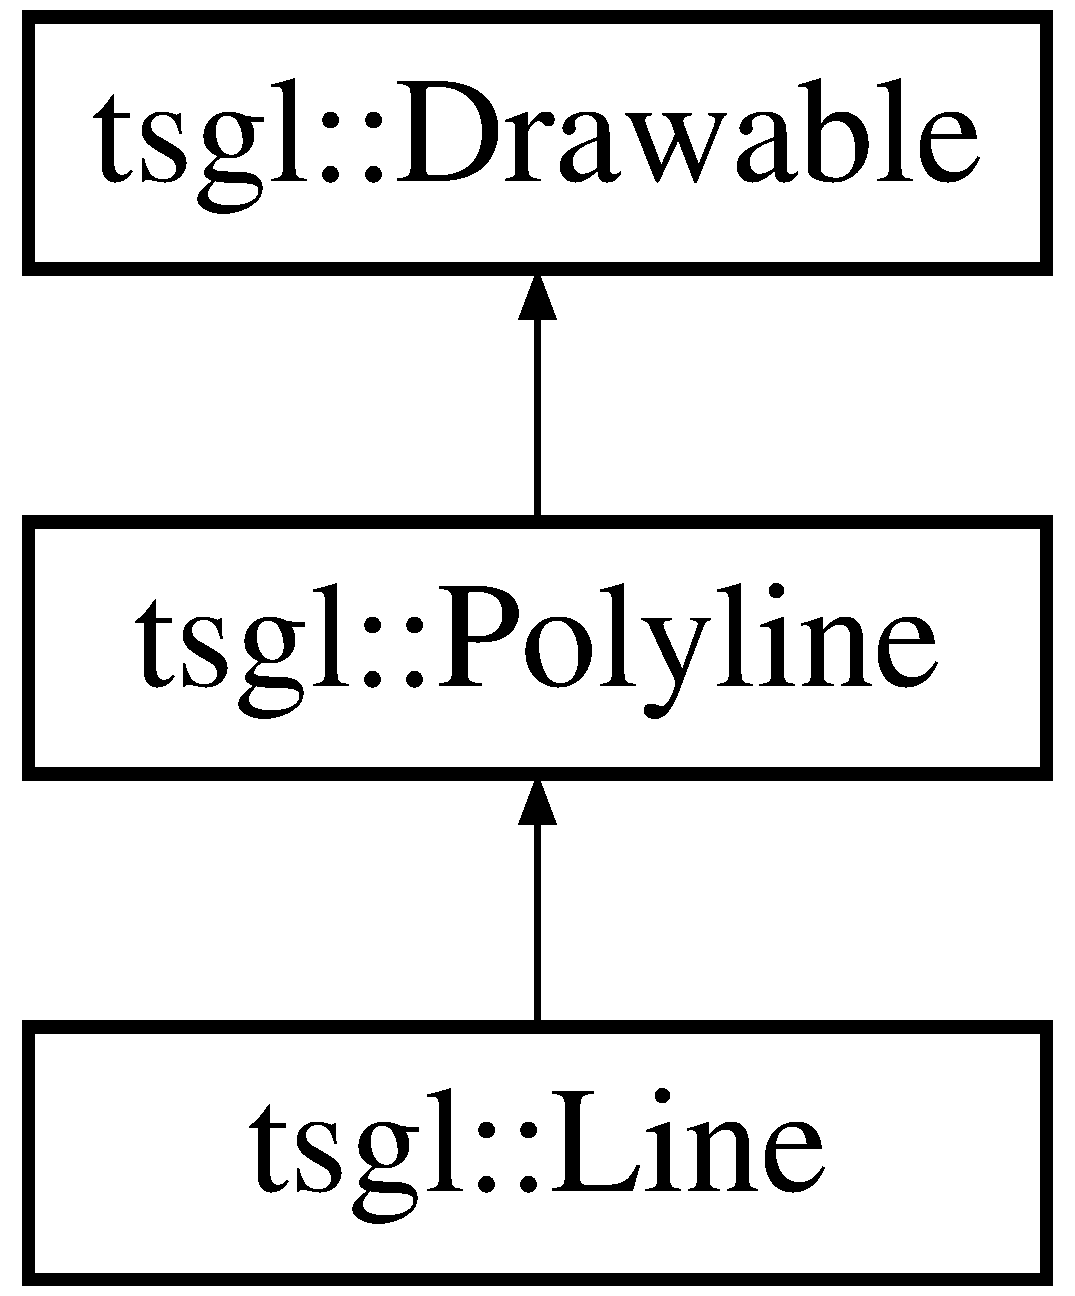
\includegraphics[height=2.000000cm]{classtsgl_1_1_polyline}
\end{center}
\end{figure}
\subsection*{Public Member Functions}
\begin{DoxyCompactItemize}
\item 
\hyperlink{classtsgl_1_1_polyline_ac618ba8a40d1f8fee9247264dc5e7513}{Polyline} (int num\+Vertices)
\begin{DoxyCompactList}\small\item\em Explicitly constructs a new \hyperlink{classtsgl_1_1_polyline}{Polyline}. \end{DoxyCompactList}\item 
\hyperlink{classtsgl_1_1_polyline_a5e186f8a65dae833d123480552b0eaad}{$\sim$\+Polyline} ()
\begin{DoxyCompactList}\small\item\em Destroys a \hyperlink{classtsgl_1_1_line}{Line} object. \end{DoxyCompactList}\item 
void \hyperlink{classtsgl_1_1_polyline_ab6598c7f60e57d9b988b19e90123da53}{add\+Next\+Vertex} (int x, int y, const \hyperlink{structtsgl_1_1_color_float}{Color\+Float} \&color=B\+L\+A\+C\+K)
\begin{DoxyCompactList}\small\item\em Adds another vertex to a \hyperlink{classtsgl_1_1_polyline}{Polyline}. \end{DoxyCompactList}\item 
void \hyperlink{classtsgl_1_1_polyline_ac6de5e2817824d9427d02d3e7be37f47}{draw} ()
\begin{DoxyCompactList}\small\item\em Draw the \hyperlink{classtsgl_1_1_polyline}{Polyline}. \end{DoxyCompactList}\end{DoxyCompactItemize}
\subsection*{Additional Inherited Members}


\subsection{Detailed Description}
Draw multiple lines chained together. 

\hyperlink{classtsgl_1_1_polyline}{Polyline} is a class for holding vertex data for multiple lines whose endpoints are connected.

This method is optimized for long lists and offers a marked improvement over drawing individual \hyperlink{classtsgl_1_1_line}{Line} instances. \begin{DoxyNote}{Note}
The add\+Vertex() method must be called the same number of times as specified in the constructor. 

Calling add\+Vertex() after all vertices have been added will do nothing. 

Calling \hyperlink{classtsgl_1_1_polyline_ac6de5e2817824d9427d02d3e7be37f47}{draw()} before all vertices have been added will do nothing. 
\end{DoxyNote}


\subsection{Constructor \& Destructor Documentation}
\hypertarget{classtsgl_1_1_polyline_ac618ba8a40d1f8fee9247264dc5e7513}{}\index{tsgl\+::\+Polyline@{tsgl\+::\+Polyline}!Polyline@{Polyline}}
\index{Polyline@{Polyline}!tsgl\+::\+Polyline@{tsgl\+::\+Polyline}}
\subsubsection[{Polyline}]{\setlength{\rightskip}{0pt plus 5cm}tsgl\+::\+Polyline\+::\+Polyline (
\begin{DoxyParamCaption}
\item[{int}]{num\+Vertices}
\end{DoxyParamCaption}
)}\label{classtsgl_1_1_polyline_ac618ba8a40d1f8fee9247264dc5e7513}


Explicitly constructs a new \hyperlink{classtsgl_1_1_polyline}{Polyline}. 

Explicit constructor for a new \hyperlink{classtsgl_1_1_polyline}{Polyline} object. 
\begin{DoxyParams}{Parameters}
{\em num\+Vertices} & The number of vertices the complete \hyperlink{classtsgl_1_1_polyline}{Polyline} will have. \\
\hline
\end{DoxyParams}
\begin{DoxyWarning}{Warning}
An invariant is held where if v is less than 2 then an error message is given. 
\end{DoxyWarning}
\begin{DoxyReturn}{Returns}
A new \hyperlink{classtsgl_1_1_polyline}{Polyline} with a buffer for storing the specified numbered of vertices. 
\end{DoxyReturn}
\hypertarget{classtsgl_1_1_polyline_a5e186f8a65dae833d123480552b0eaad}{}\index{tsgl\+::\+Polyline@{tsgl\+::\+Polyline}!````~Polyline@{$\sim$\+Polyline}}
\index{````~Polyline@{$\sim$\+Polyline}!tsgl\+::\+Polyline@{tsgl\+::\+Polyline}}
\subsubsection[{$\sim$\+Polyline}]{\setlength{\rightskip}{0pt plus 5cm}tsgl\+::\+Polyline\+::$\sim$\+Polyline (
\begin{DoxyParamCaption}
{}
\end{DoxyParamCaption}
)}\label{classtsgl_1_1_polyline_a5e186f8a65dae833d123480552b0eaad}


Destroys a \hyperlink{classtsgl_1_1_line}{Line} object. 

Destructor for a \hyperlink{classtsgl_1_1_line}{Line} object.

Frees up memory allocated to a \hyperlink{classtsgl_1_1_line}{Line} object. 

\subsection{Member Function Documentation}
\hypertarget{classtsgl_1_1_polyline_ab6598c7f60e57d9b988b19e90123da53}{}\index{tsgl\+::\+Polyline@{tsgl\+::\+Polyline}!add\+Next\+Vertex@{add\+Next\+Vertex}}
\index{add\+Next\+Vertex@{add\+Next\+Vertex}!tsgl\+::\+Polyline@{tsgl\+::\+Polyline}}
\subsubsection[{add\+Next\+Vertex}]{\setlength{\rightskip}{0pt plus 5cm}void tsgl\+::\+Polyline\+::add\+Next\+Vertex (
\begin{DoxyParamCaption}
\item[{int}]{x, }
\item[{int}]{y, }
\item[{const {\bf Color\+Float} \&}]{color = {\ttfamily BLACK}}
\end{DoxyParamCaption}
)}\label{classtsgl_1_1_polyline_ab6598c7f60e57d9b988b19e90123da53}


Adds another vertex to a \hyperlink{classtsgl_1_1_polyline}{Polyline}. 

This function initializes the next vertex in a \hyperlink{classtsgl_1_1_polyline}{Polyline} and adds it to the \hyperlink{classtsgl_1_1_polyline}{Polyline}\textquotesingle{}s buffer. 
\begin{DoxyParams}{Parameters}
{\em x} & The x position of the vertex. \\
\hline
{\em y} & The y position of the vertex. \\
\hline
{\em color} & The reference variable to the color of the vertex (set to B\+L\+A\+C\+K by default). \\
\hline
\end{DoxyParams}
\begin{DoxyNote}{Note}
This function does nothing if the vertex buffer is already full. 

A message is given indicating when the vertex buffer is full. 
\end{DoxyNote}


Referenced by tsgl\+::\+Canvas\+::draw\+Circle(), tsgl\+::\+Canvas\+::draw\+Colored\+Polygon(), tsgl\+::\+Canvas\+::draw\+Concave\+Polygon(), tsgl\+::\+Canvas\+::draw\+Convex\+Polygon(), tsgl\+::\+Cartesian\+Canvas\+::draw\+Function(), tsgl\+::\+Canvas\+::draw\+Rectangle(), tsgl\+::\+Canvas\+::draw\+Triangle(), and tsgl\+::\+Progress\+Bar\+::get\+Border().

\hypertarget{classtsgl_1_1_polyline_ac6de5e2817824d9427d02d3e7be37f47}{}\index{tsgl\+::\+Polyline@{tsgl\+::\+Polyline}!draw@{draw}}
\index{draw@{draw}!tsgl\+::\+Polyline@{tsgl\+::\+Polyline}}
\subsubsection[{draw}]{\setlength{\rightskip}{0pt plus 5cm}void tsgl\+::\+Polyline\+::draw (
\begin{DoxyParamCaption}
{}
\end{DoxyParamCaption}
)\hspace{0.3cm}{\ttfamily [virtual]}}\label{classtsgl_1_1_polyline_ac6de5e2817824d9427d02d3e7be37f47}


Draw the \hyperlink{classtsgl_1_1_polyline}{Polyline}. 

This function actually draws the \hyperlink{classtsgl_1_1_polyline}{Polyline} to the \hyperlink{classtsgl_1_1_canvas}{Canvas}. \begin{DoxyNote}{Note}
This function does nothing if the vertex buffer is not yet full. 

A message indicating that the \hyperlink{classtsgl_1_1_polyline}{Polyline} cannot be drawn yet will be given if the above condition is met (vertex buffer = not full). 
\end{DoxyNote}


Implements \hyperlink{classtsgl_1_1_shape_af78b1627b97d621824ce86db214e2402}{tsgl\+::\+Shape}.



The documentation for this class was generated from the following files\+:\begin{DoxyCompactItemize}
\item 
Polyline.\+h\item 
Polyline.\+cpp\end{DoxyCompactItemize}

\hypertarget{class_pong}{}\section{Pong Class Reference}
\label{class_pong}\index{Pong@{Pong}}


An old-\/school classic!  




{\ttfamily \#include $<$Pong.\+h$>$}

\subsection*{Public Member Functions}
\begin{DoxyCompactItemize}
\item 
\hyperlink{class_pong_afc1bb4388485aeb675c3d2a854c8baf6}{Pong} (\hyperlink{classtsgl_1_1_canvas}{Canvas} \&can, int \&ball\+Speed, int \&paddle\+Speed)
\begin{DoxyCompactList}\small\item\em Explicitly construct the game, \hyperlink{class_pong}{Pong}. \end{DoxyCompactList}\item 
void \hyperlink{class_pong_a3c7242248be0e6980595faaa0a927866}{draw} (\hyperlink{classtsgl_1_1_canvas}{Canvas} \&can)
\begin{DoxyCompactList}\small\item\em Draw the game of \hyperlink{class_pong}{Pong}. \end{DoxyCompactList}\item 
\mbox{\Hypertarget{class_pong_a51b1a3feee45026071eaba47489e504a}\label{class_pong_a51b1a3feee45026071eaba47489e504a}} 
\hyperlink{class_pong_a51b1a3feee45026071eaba47489e504a}{$\sim$\+Pong} ()
\begin{DoxyCompactList}\small\item\em Destroys the \hyperlink{class_pong}{Pong} game object. \end{DoxyCompactList}\end{DoxyCompactItemize}


\subsection{Detailed Description}
An old-\/school classic! 

Draw the interactive game of \hyperlink{class_pong}{Pong}. The two paddles are objects and the ball is also an object.

The constructor constructs the two paddle objects and the ball object.

Use the W and S keys in order to move the left paddle, the Up and Down arrow keys in order to move the right paddle.

Everything else is handled in the \hyperlink{class_pong_a3c7242248be0e6980595faaa0a927866}{draw()} method (button bindings, score keeping, drawing the objects and the game itself, ball collisions with the paddles and the boundaries). \begin{DoxySeeAlso}{See also}
\hyperlink{class_paddle}{Paddle} class, \hyperlink{class_ball}{Ball} class. 
\end{DoxySeeAlso}


\subsection{Constructor \& Destructor Documentation}
\mbox{\Hypertarget{class_pong_afc1bb4388485aeb675c3d2a854c8baf6}\label{class_pong_afc1bb4388485aeb675c3d2a854c8baf6}} 
\index{Pong@{Pong}!Pong@{Pong}}
\index{Pong@{Pong}!Pong@{Pong}}
\subsubsection{\texorpdfstring{Pong()}{Pong()}}
{\footnotesize\ttfamily Pong\+::\+Pong (\begin{DoxyParamCaption}\item[{\hyperlink{classtsgl_1_1_canvas}{Canvas} \&}]{can,  }\item[{int \&}]{ball\+Speed,  }\item[{int \&}]{paddle\+Speed }\end{DoxyParamCaption})}



Explicitly construct the game, \hyperlink{class_pong}{Pong}. 

Explicit constructor for the game, \hyperlink{class_pong}{Pong}. It sets up the \hyperlink{class_paddle}{Paddle} objects and the \hyperlink{class_ball}{Ball} object in order to play. 
\begin{DoxyParams}{Parameters}
{\em can} & Reference to the Canvas to use when playing \hyperlink{class_pong}{Pong}. \\
\hline
{\em ball\+Speed} & Reference to the ball speed to use in the game. \\
\hline
{\em paddle\+Speed} & Reference to the paddle speed to use in the game. \\
\hline
\end{DoxyParams}


\subsection{Member Function Documentation}
\mbox{\Hypertarget{class_pong_a3c7242248be0e6980595faaa0a927866}\label{class_pong_a3c7242248be0e6980595faaa0a927866}} 
\index{Pong@{Pong}!draw@{draw}}
\index{draw@{draw}!Pong@{Pong}}
\subsubsection{\texorpdfstring{draw()}{draw()}}
{\footnotesize\ttfamily void Pong\+::draw (\begin{DoxyParamCaption}\item[{\hyperlink{classtsgl_1_1_canvas}{Canvas} \&}]{can }\end{DoxyParamCaption})}



Draw the game of \hyperlink{class_pong}{Pong}. 

Actually draws all of the necessary components in order to play \hyperlink{class_pong}{Pong}. This also includes any necessary button bindings in order to move the \hyperlink{class_paddle}{Paddle} objects. 
\begin{DoxyParams}{Parameters}
{\em can} & Reference to the Canvas to draw on. \\
\hline
\end{DoxyParams}
\begin{DoxySeeAlso}{See also}
\hyperlink{class_paddle}{Paddle} class, \hyperlink{class_ball}{Ball} class. 
\end{DoxySeeAlso}


The documentation for this class was generated from the following files\+:\begin{DoxyCompactItemize}
\item 
/home/sth5/test/\+T\+S\+G\+L/src/examples/\+Pong/Pong.\+h\item 
/home/sth5/test/\+T\+S\+G\+L/src/examples/\+Pong/Pong.\+cpp\end{DoxyCompactItemize}

\hypertarget{classtsgl_1_1_power_function}{}\section{tsgl\+:\+:Power\+Function Class Reference}
\label{classtsgl_1_1_power_function}\index{tsgl\+::\+Power\+Function@{tsgl\+::\+Power\+Function}}


\hyperlink{classtsgl_1_1_function}{Function} to compute the input raised to a specified power.  




{\ttfamily \#include $<$Function.\+h$>$}

Inheritance diagram for tsgl\+:\+:Power\+Function\+:\begin{figure}[H]
\begin{center}
\leavevmode
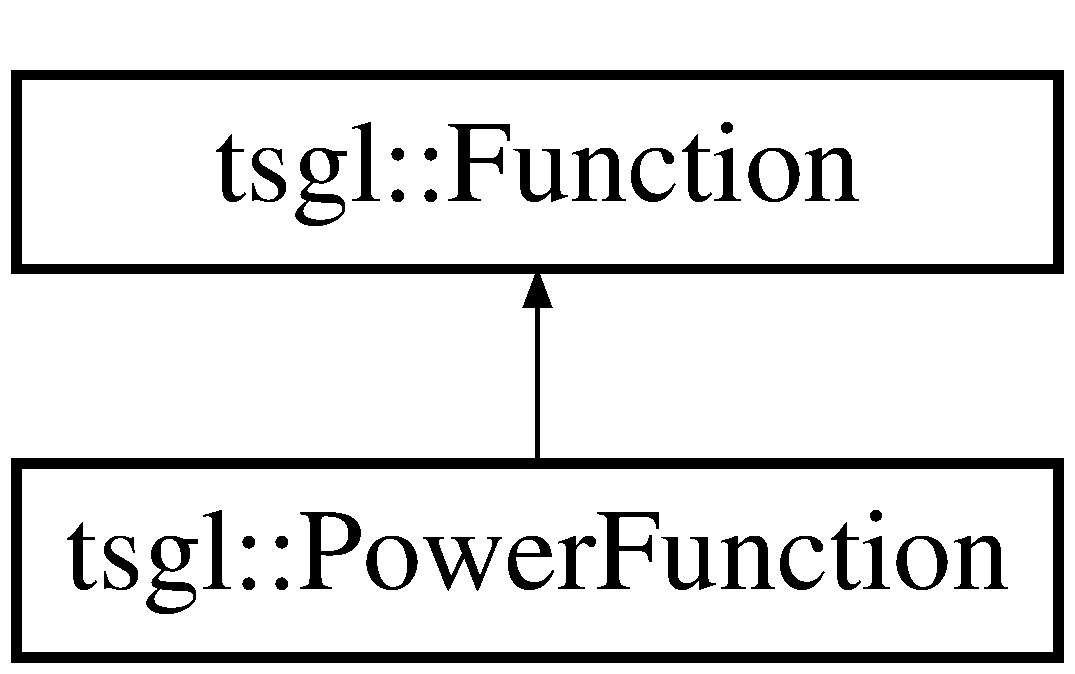
\includegraphics[height=2.000000cm]{classtsgl_1_1_power_function}
\end{center}
\end{figure}
\subsection*{Public Member Functions}
\begin{DoxyCompactItemize}
\item 
\hyperlink{classtsgl_1_1_power_function_a0a5d692e9bc9cf2a176ecab4ffc06519}{Power\+Function} (Decimal a)
\begin{DoxyCompactList}\small\item\em Constructs a new \hyperlink{classtsgl_1_1_power_function}{Power\+Function}. \end{DoxyCompactList}\item 
virtual Decimal \hyperlink{classtsgl_1_1_power_function_ae63821b4c2347508c42c300a0c306076}{value\+At} (Decimal x) const 
\begin{DoxyCompactList}\small\item\em Method to determine the value of \hyperlink{classtsgl_1_1_power_function}{Power\+Function}. \end{DoxyCompactList}\end{DoxyCompactItemize}


\subsection{Detailed Description}
\hyperlink{classtsgl_1_1_function}{Function} to compute the input raised to a specified power. 

\subsection{Constructor \& Destructor Documentation}
\hypertarget{classtsgl_1_1_power_function_a0a5d692e9bc9cf2a176ecab4ffc06519}{}\index{tsgl\+::\+Power\+Function@{tsgl\+::\+Power\+Function}!Power\+Function@{Power\+Function}}
\index{Power\+Function@{Power\+Function}!tsgl\+::\+Power\+Function@{tsgl\+::\+Power\+Function}}
\subsubsection[{Power\+Function}]{\setlength{\rightskip}{0pt plus 5cm}tsgl\+::\+Power\+Function\+::\+Power\+Function (
\begin{DoxyParamCaption}
\item[{Decimal}]{a}
\end{DoxyParamCaption}
)\hspace{0.3cm}{\ttfamily [inline]}}\label{classtsgl_1_1_power_function_a0a5d692e9bc9cf2a176ecab4ffc06519}


Constructs a new \hyperlink{classtsgl_1_1_power_function}{Power\+Function}. 


\begin{DoxyParams}{Parameters}
{\em a} & The power to which the input is raised. \\
\hline
\end{DoxyParams}


\subsection{Member Function Documentation}
\hypertarget{classtsgl_1_1_power_function_ae63821b4c2347508c42c300a0c306076}{}\index{tsgl\+::\+Power\+Function@{tsgl\+::\+Power\+Function}!value\+At@{value\+At}}
\index{value\+At@{value\+At}!tsgl\+::\+Power\+Function@{tsgl\+::\+Power\+Function}}
\subsubsection[{value\+At}]{\setlength{\rightskip}{0pt plus 5cm}virtual Decimal tsgl\+::\+Power\+Function\+::value\+At (
\begin{DoxyParamCaption}
\item[{Decimal}]{x}
\end{DoxyParamCaption}
) const\hspace{0.3cm}{\ttfamily [inline]}, {\ttfamily [virtual]}}\label{classtsgl_1_1_power_function_ae63821b4c2347508c42c300a0c306076}


Method to determine the value of \hyperlink{classtsgl_1_1_power_function}{Power\+Function}. 


\begin{DoxyParams}{Parameters}
{\em x} & The input to the function. \\
\hline
\end{DoxyParams}
\begin{DoxyReturn}{Returns}
{\itshape x} raised to the $\ast$a$\ast$th power. 
\end{DoxyReturn}


Implements \hyperlink{classtsgl_1_1_function_affb7b3b19a04efefa29a9870d666e912}{tsgl\+::\+Function}.



The documentation for this class was generated from the following file\+:\begin{DoxyCompactItemize}
\item 
Function.\+h\end{DoxyCompactItemize}

\hypertarget{classtsgl_1_1_prism}{}\section{tsgl\+:\+:Prism Class Reference}
\label{classtsgl_1_1_prism}\index{tsgl\+::\+Prism@{tsgl\+::\+Prism}}


Draw an arbitrary \hyperlink{classtsgl_1_1_prism}{Prism} with colored vertices.  




{\ttfamily \#include $<$Prism.\+h$>$}

Inheritance diagram for tsgl\+:\+:Prism\+:\begin{figure}[H]
\begin{center}
\leavevmode
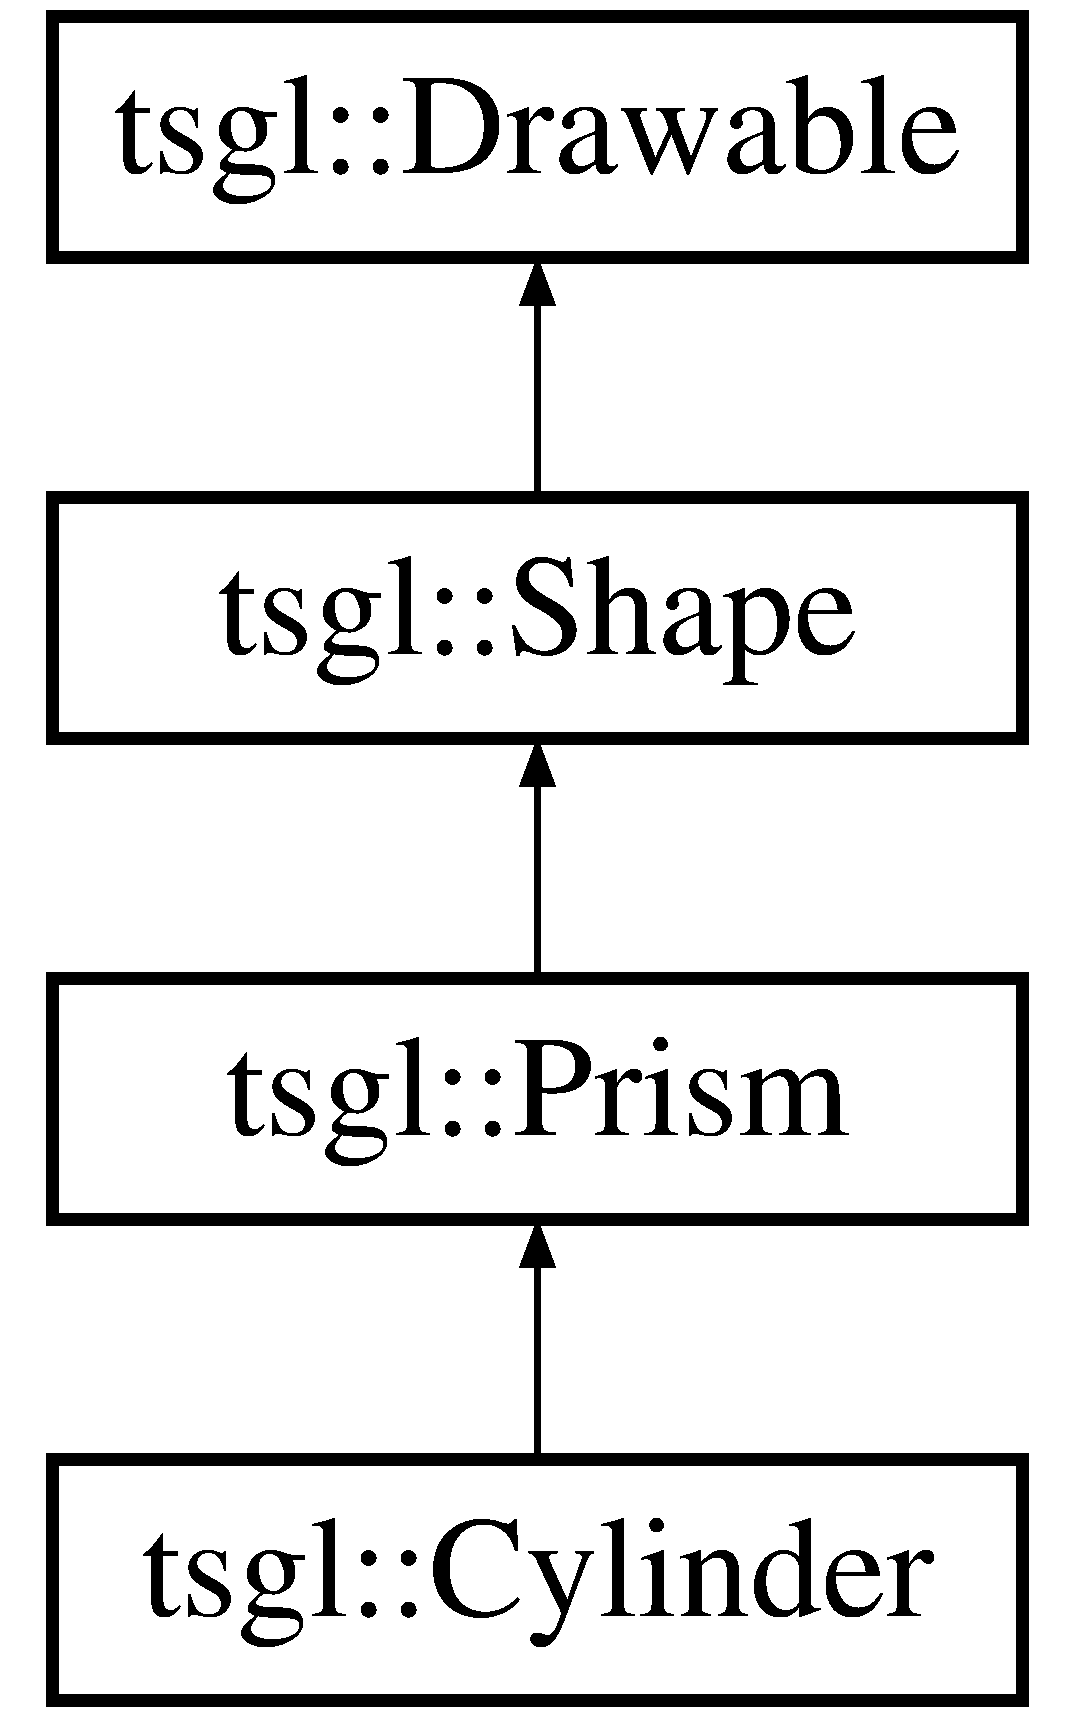
\includegraphics[height=4.000000cm]{classtsgl_1_1_prism}
\end{center}
\end{figure}
\subsection*{Public Member Functions}
\begin{DoxyCompactItemize}
\item 
\hyperlink{classtsgl_1_1_prism_a4e4b0cdd81d76d48f032a691df2d81c2}{Prism} (float x, float y, float z, int sides, G\+Lfloat height, G\+Lfloat radius, float yaw, float pitch, float roll, \hyperlink{structtsgl_1_1_color_float}{Color\+Float} c)
\begin{DoxyCompactList}\small\item\em Explicitly constructs a new \hyperlink{classtsgl_1_1_prism}{Prism}. \end{DoxyCompactList}\item 
\hyperlink{classtsgl_1_1_prism_a665fe3ba2d8c0255b0090170ac5bc643}{Prism} (float x, float y, float z, int sides, G\+Lfloat height, G\+Lfloat radius, float yaw, float pitch, float roll, \hyperlink{structtsgl_1_1_color_float}{Color\+Float} c\mbox{[}$\,$\mbox{]})
\begin{DoxyCompactList}\small\item\em Explicitly constructs a new \hyperlink{classtsgl_1_1_prism}{Prism}. \end{DoxyCompactList}\item 
virtual void \hyperlink{classtsgl_1_1_prism_a33bc4c80ac4d5cbb8c33a657fca01524}{set\+Height} (G\+Lfloat height)
\begin{DoxyCompactList}\small\item\em Mutates the distance from the \hyperlink{classtsgl_1_1_prism}{Prism}\textquotesingle{}s bottom to its top. \end{DoxyCompactList}\item 
virtual void \hyperlink{classtsgl_1_1_prism_a97e94e9e2b395f604573bcb5ef646f15}{change\+Height\+By} (G\+Lfloat delta)
\begin{DoxyCompactList}\small\item\em Mutates the distance from the \hyperlink{classtsgl_1_1_prism}{Prism}\textquotesingle{}s bottom to its top by the parameter amount. \end{DoxyCompactList}\item 
virtual void \hyperlink{classtsgl_1_1_prism_afab75920c51c0104d20f78534fac3656}{set\+Radius} (G\+Lfloat radius)
\begin{DoxyCompactList}\small\item\em Mutates the distance from the center of the \hyperlink{classtsgl_1_1_prism}{Prism}\textquotesingle{}s base to the corners. \end{DoxyCompactList}\item 
virtual void \hyperlink{classtsgl_1_1_prism_ae16f2d46d3fb263d389bfcc2a45bda63}{change\+Radius\+By} (G\+Lfloat delta)
\begin{DoxyCompactList}\small\item\em Mutates the distance from the center of the \hyperlink{classtsgl_1_1_prism}{Prism}\textquotesingle{}s base to the corner by the parameter amount. \end{DoxyCompactList}\item 
virtual G\+Lfloat \hyperlink{classtsgl_1_1_prism_a65f06653960000dc544a0348fe979171}{get\+Radius} ()
\begin{DoxyCompactList}\small\item\em Accessor for the radius of the \hyperlink{classtsgl_1_1_prism}{Prism}. \end{DoxyCompactList}\item 
virtual G\+Lfloat \hyperlink{classtsgl_1_1_prism_a5a62be4c54080aa3171d8bf9a2d9caf0}{get\+Height} ()
\begin{DoxyCompactList}\small\item\em Accessor for the height of the \hyperlink{classtsgl_1_1_prism}{Prism}. \end{DoxyCompactList}\item 
virtual void \hyperlink{classtsgl_1_1_prism_af2c681fd9cf74eaede3dd4fd8dd10625}{set\+Color} (\hyperlink{structtsgl_1_1_color_float}{Color\+Float} c)
\begin{DoxyCompactList}\small\item\em Sets the \hyperlink{classtsgl_1_1_shape}{Shape} to a new color. \end{DoxyCompactList}\item 
virtual void \hyperlink{classtsgl_1_1_prism_a668c2779da173493efc0c4634750bd66}{set\+Color} (\hyperlink{structtsgl_1_1_color_float}{Color\+Float} c\mbox{[}$\,$\mbox{]})
\begin{DoxyCompactList}\small\item\em Mutator. Sets the \hyperlink{classtsgl_1_1_prism}{Prism} to a new array of colors. \end{DoxyCompactList}\item 
virtual void \hyperlink{classtsgl_1_1_prism_abfdc091d8c61e889f61b71577b58e0b6}{get\+Colors} (std\+::vector$<$ \hyperlink{structtsgl_1_1_color_float}{Color\+Float} $>$ \&color\+Vec)
\begin{DoxyCompactList}\small\item\em Accessor for \hyperlink{classtsgl_1_1_arrow}{Arrow}\textquotesingle{}s colors. \end{DoxyCompactList}\end{DoxyCompactItemize}
\subsection*{Protected Attributes}
\begin{DoxyCompactItemize}
\item 
\mbox{\Hypertarget{classtsgl_1_1_prism_a09331661d18ef6d374b4bc5a7660a1c6}\label{classtsgl_1_1_prism_a09331661d18ef6d374b4bc5a7660a1c6}} 
G\+Lfloat {\bfseries my\+Height}
\item 
\mbox{\Hypertarget{classtsgl_1_1_prism_af5cc843f733123fe64b464ba45249d62}\label{classtsgl_1_1_prism_af5cc843f733123fe64b464ba45249d62}} 
G\+Lfloat {\bfseries my\+Radius}
\item 
\mbox{\Hypertarget{classtsgl_1_1_prism_aa2b47e0792014dcca133846050b077ba}\label{classtsgl_1_1_prism_aa2b47e0792014dcca133846050b077ba}} 
int {\bfseries my\+Sides}
\end{DoxyCompactItemize}
\subsection*{Additional Inherited Members}


\subsection{Detailed Description}
Draw an arbitrary \hyperlink{classtsgl_1_1_prism}{Prism} with colored vertices. 

\hyperlink{classtsgl_1_1_prism}{Prism} is a class for holding vertex data for a \hyperlink{classtsgl_1_1_prism}{Prism} with a base with at least 3 sides. 

\subsection{Constructor \& Destructor Documentation}
\mbox{\Hypertarget{classtsgl_1_1_prism_a4e4b0cdd81d76d48f032a691df2d81c2}\label{classtsgl_1_1_prism_a4e4b0cdd81d76d48f032a691df2d81c2}} 
\index{tsgl\+::\+Prism@{tsgl\+::\+Prism}!Prism@{Prism}}
\index{Prism@{Prism}!tsgl\+::\+Prism@{tsgl\+::\+Prism}}
\subsubsection{\texorpdfstring{Prism()}{Prism()}\hspace{0.1cm}{\footnotesize\ttfamily [1/2]}}
{\footnotesize\ttfamily tsgl\+::\+Prism\+::\+Prism (\begin{DoxyParamCaption}\item[{float}]{x,  }\item[{float}]{y,  }\item[{float}]{z,  }\item[{int}]{sides,  }\item[{G\+Lfloat}]{height,  }\item[{G\+Lfloat}]{radius,  }\item[{float}]{yaw,  }\item[{float}]{pitch,  }\item[{float}]{roll,  }\item[{\hyperlink{structtsgl_1_1_color_float}{Color\+Float}}]{c }\end{DoxyParamCaption})}



Explicitly constructs a new \hyperlink{classtsgl_1_1_prism}{Prism}. 

Explicit constructor for a \hyperlink{classtsgl_1_1_prism}{Prism} object. 
\begin{DoxyParams}{Parameters}
{\em x} & The x coordinate of the center of the \hyperlink{classtsgl_1_1_prism}{Prism}. \\
\hline
{\em y} & The y coordinate of the center of the \hyperlink{classtsgl_1_1_prism}{Prism}. \\
\hline
{\em z} & The z coordinate of the center of the \hyperlink{classtsgl_1_1_prism}{Prism}. \\
\hline
{\em sides} & The number of sides of the \hyperlink{classtsgl_1_1_prism}{Prism}\textquotesingle{}s base. \\
\hline
{\em yaw} & The \hyperlink{classtsgl_1_1_prism}{Prism}\textquotesingle{}s yaw. \\
\hline
{\em pitch} & The \hyperlink{classtsgl_1_1_prism}{Prism}\textquotesingle{}s pitch. \\
\hline
{\em roll} & The \hyperlink{classtsgl_1_1_prism}{Prism}\textquotesingle{}s roll. \\
\hline
{\em c} & A \hyperlink{structtsgl_1_1_color_float}{Color\+Float} for the \hyperlink{classtsgl_1_1_prism}{Prism}\textquotesingle{}s vertex colors. \\
\hline
\end{DoxyParams}
\begin{DoxyWarning}{Warning}
An invariant is held where if sides is less than 3 then an error message is given. 

An invariant is held where if radius isn\textquotesingle{}t positive then an error message is given. 

An invariant is held where if all points in vertices are not in the same plane then an error message is given. 
\end{DoxyWarning}
\begin{DoxyReturn}{Returns}
A new \hyperlink{classtsgl_1_1_prism}{Prism} with a buffer for storing the specified numbered of vertices. 
\end{DoxyReturn}


Referenced by tsgl\+::\+Cylinder\+::\+Cylinder().

\mbox{\Hypertarget{classtsgl_1_1_prism_a665fe3ba2d8c0255b0090170ac5bc643}\label{classtsgl_1_1_prism_a665fe3ba2d8c0255b0090170ac5bc643}} 
\index{tsgl\+::\+Prism@{tsgl\+::\+Prism}!Prism@{Prism}}
\index{Prism@{Prism}!tsgl\+::\+Prism@{tsgl\+::\+Prism}}
\subsubsection{\texorpdfstring{Prism()}{Prism()}\hspace{0.1cm}{\footnotesize\ttfamily [2/2]}}
{\footnotesize\ttfamily tsgl\+::\+Prism\+::\+Prism (\begin{DoxyParamCaption}\item[{float}]{x,  }\item[{float}]{y,  }\item[{float}]{z,  }\item[{int}]{sides,  }\item[{G\+Lfloat}]{height,  }\item[{G\+Lfloat}]{radius,  }\item[{float}]{yaw,  }\item[{float}]{pitch,  }\item[{float}]{roll,  }\item[{\hyperlink{structtsgl_1_1_color_float}{Color\+Float}}]{c\mbox{[}$\,$\mbox{]} }\end{DoxyParamCaption})}



Explicitly constructs a new \hyperlink{classtsgl_1_1_prism}{Prism}. 

Explicit constructor for a \hyperlink{classtsgl_1_1_prism}{Prism} object. 
\begin{DoxyParams}{Parameters}
{\em x} & The x coordinate of the center of the \hyperlink{classtsgl_1_1_prism}{Prism}. \\
\hline
{\em y} & The y coordinate of the center of the \hyperlink{classtsgl_1_1_prism}{Prism}. \\
\hline
{\em z} & The z coordinate of the center of the \hyperlink{classtsgl_1_1_prism}{Prism}. \\
\hline
{\em sides} & The number of sides of the \hyperlink{classtsgl_1_1_prism}{Prism}\textquotesingle{}s base. \\
\hline
{\em yaw} & The \hyperlink{classtsgl_1_1_prism}{Prism}\textquotesingle{}s yaw. \\
\hline
{\em pitch} & The \hyperlink{classtsgl_1_1_prism}{Prism}\textquotesingle{}s pitch. \\
\hline
{\em roll} & The \hyperlink{classtsgl_1_1_prism}{Prism}\textquotesingle{}s roll. \\
\hline
{\em c} & An array of Color\+Floats for the \hyperlink{classtsgl_1_1_prism}{Prism}\textquotesingle{}s vertex colors. \\
\hline
\end{DoxyParams}
\begin{DoxyWarning}{Warning}
An invariant is held where if sides is less than 3 then an error message is given. 

An invariant is held where if radius isn\textquotesingle{}t positive then an error message is given. 

An invariant is held where if all points in vertices are not in the same plane then an error message is given. 
\end{DoxyWarning}
\begin{DoxyReturn}{Returns}
A new \hyperlink{classtsgl_1_1_prism}{Prism} with a buffer for storing the specified numbered of vertices. 
\end{DoxyReturn}


\subsection{Member Function Documentation}
\mbox{\Hypertarget{classtsgl_1_1_prism_a97e94e9e2b395f604573bcb5ef646f15}\label{classtsgl_1_1_prism_a97e94e9e2b395f604573bcb5ef646f15}} 
\index{tsgl\+::\+Prism@{tsgl\+::\+Prism}!change\+Height\+By@{change\+Height\+By}}
\index{change\+Height\+By@{change\+Height\+By}!tsgl\+::\+Prism@{tsgl\+::\+Prism}}
\subsubsection{\texorpdfstring{change\+Height\+By()}{changeHeightBy()}}
{\footnotesize\ttfamily void tsgl\+::\+Prism\+::change\+Height\+By (\begin{DoxyParamCaption}\item[{G\+Lfloat}]{delta }\end{DoxyParamCaption})\hspace{0.3cm}{\ttfamily [virtual]}}



Mutates the distance from the \hyperlink{classtsgl_1_1_prism}{Prism}\textquotesingle{}s bottom to its top by the parameter amount. 


\begin{DoxyParams}{Parameters}
{\em delta} & The amount by which to change the height of the \hyperlink{classtsgl_1_1_prism}{Prism}. \\
\hline
\end{DoxyParams}
\mbox{\Hypertarget{classtsgl_1_1_prism_ae16f2d46d3fb263d389bfcc2a45bda63}\label{classtsgl_1_1_prism_ae16f2d46d3fb263d389bfcc2a45bda63}} 
\index{tsgl\+::\+Prism@{tsgl\+::\+Prism}!change\+Radius\+By@{change\+Radius\+By}}
\index{change\+Radius\+By@{change\+Radius\+By}!tsgl\+::\+Prism@{tsgl\+::\+Prism}}
\subsubsection{\texorpdfstring{change\+Radius\+By()}{changeRadiusBy()}}
{\footnotesize\ttfamily void tsgl\+::\+Prism\+::change\+Radius\+By (\begin{DoxyParamCaption}\item[{G\+Lfloat}]{delta }\end{DoxyParamCaption})\hspace{0.3cm}{\ttfamily [virtual]}}



Mutates the distance from the center of the \hyperlink{classtsgl_1_1_prism}{Prism}\textquotesingle{}s base to the corner by the parameter amount. 


\begin{DoxyParams}{Parameters}
{\em delta} & The amount by which to change the radius of the \hyperlink{classtsgl_1_1_prism}{Prism}. \\
\hline
\end{DoxyParams}
\mbox{\Hypertarget{classtsgl_1_1_prism_abfdc091d8c61e889f61b71577b58e0b6}\label{classtsgl_1_1_prism_abfdc091d8c61e889f61b71577b58e0b6}} 
\index{tsgl\+::\+Prism@{tsgl\+::\+Prism}!get\+Colors@{get\+Colors}}
\index{get\+Colors@{get\+Colors}!tsgl\+::\+Prism@{tsgl\+::\+Prism}}
\subsubsection{\texorpdfstring{get\+Colors()}{getColors()}}
{\footnotesize\ttfamily void tsgl\+::\+Prism\+::get\+Colors (\begin{DoxyParamCaption}\item[{std\+::vector$<$ \hyperlink{structtsgl_1_1_color_float}{Color\+Float} $>$ \&}]{color\+Vec }\end{DoxyParamCaption})\hspace{0.3cm}{\ttfamily [virtual]}}



Accessor for \hyperlink{classtsgl_1_1_arrow}{Arrow}\textquotesingle{}s colors. 

Populates the reference parameter vector with a \hyperlink{structtsgl_1_1_color_float}{Color\+Float} for each end of \hyperlink{classtsgl_1_1_arrow}{Arrow}. 
\begin{DoxyParams}{Parameters}
{\em color\+Vec} & A vector of Color\+Floats to which the Color\+Floats associated with \hyperlink{classtsgl_1_1_arrow}{Arrow} will be pushed. \\
\hline
\end{DoxyParams}
\begin{DoxyNote}{Note}
Overrides \hyperlink{classtsgl_1_1_shape_a6f54fe4d049f69a287edf8335a9509f8}{Shape\+::get\+Colors()}. 
\end{DoxyNote}


Reimplemented from \hyperlink{classtsgl_1_1_shape_a6f54fe4d049f69a287edf8335a9509f8}{tsgl\+::\+Shape}.



Referenced by set\+Color().

\mbox{\Hypertarget{classtsgl_1_1_prism_a5a62be4c54080aa3171d8bf9a2d9caf0}\label{classtsgl_1_1_prism_a5a62be4c54080aa3171d8bf9a2d9caf0}} 
\index{tsgl\+::\+Prism@{tsgl\+::\+Prism}!get\+Height@{get\+Height}}
\index{get\+Height@{get\+Height}!tsgl\+::\+Prism@{tsgl\+::\+Prism}}
\subsubsection{\texorpdfstring{get\+Height()}{getHeight()}}
{\footnotesize\ttfamily virtual G\+Lfloat tsgl\+::\+Prism\+::get\+Height (\begin{DoxyParamCaption}{ }\end{DoxyParamCaption})\hspace{0.3cm}{\ttfamily [inline]}, {\ttfamily [virtual]}}



Accessor for the height of the \hyperlink{classtsgl_1_1_prism}{Prism}. 

Returns the value of the my\+Height private variable, a G\+Lfloat. \mbox{\Hypertarget{classtsgl_1_1_prism_a65f06653960000dc544a0348fe979171}\label{classtsgl_1_1_prism_a65f06653960000dc544a0348fe979171}} 
\index{tsgl\+::\+Prism@{tsgl\+::\+Prism}!get\+Radius@{get\+Radius}}
\index{get\+Radius@{get\+Radius}!tsgl\+::\+Prism@{tsgl\+::\+Prism}}
\subsubsection{\texorpdfstring{get\+Radius()}{getRadius()}}
{\footnotesize\ttfamily virtual G\+Lfloat tsgl\+::\+Prism\+::get\+Radius (\begin{DoxyParamCaption}{ }\end{DoxyParamCaption})\hspace{0.3cm}{\ttfamily [inline]}, {\ttfamily [virtual]}}



Accessor for the radius of the \hyperlink{classtsgl_1_1_prism}{Prism}. 

Returns the value of the my\+Radius private variable, a G\+Lfloat. \mbox{\Hypertarget{classtsgl_1_1_prism_af2c681fd9cf74eaede3dd4fd8dd10625}\label{classtsgl_1_1_prism_af2c681fd9cf74eaede3dd4fd8dd10625}} 
\index{tsgl\+::\+Prism@{tsgl\+::\+Prism}!set\+Color@{set\+Color}}
\index{set\+Color@{set\+Color}!tsgl\+::\+Prism@{tsgl\+::\+Prism}}
\subsubsection{\texorpdfstring{set\+Color()}{setColor()}\hspace{0.1cm}{\footnotesize\ttfamily [1/2]}}
{\footnotesize\ttfamily virtual void tsgl\+::\+Prism\+::set\+Color (\begin{DoxyParamCaption}\item[{\hyperlink{structtsgl_1_1_color_float}{Color\+Float}}]{c }\end{DoxyParamCaption})\hspace{0.3cm}{\ttfamily [inline]}, {\ttfamily [virtual]}}



Sets the \hyperlink{classtsgl_1_1_shape}{Shape} to a new color. 


\begin{DoxyParams}{Parameters}
{\em c} & The new \hyperlink{structtsgl_1_1_color_float}{Color\+Float}. \\
\hline
\end{DoxyParams}


Reimplemented from \hyperlink{classtsgl_1_1_shape_abdb01321cddfd2db1481eefbc2836f70}{tsgl\+::\+Shape}.



Referenced by Philosopher3\+D\+::refresh\+Color().

\mbox{\Hypertarget{classtsgl_1_1_prism_a668c2779da173493efc0c4634750bd66}\label{classtsgl_1_1_prism_a668c2779da173493efc0c4634750bd66}} 
\index{tsgl\+::\+Prism@{tsgl\+::\+Prism}!set\+Color@{set\+Color}}
\index{set\+Color@{set\+Color}!tsgl\+::\+Prism@{tsgl\+::\+Prism}}
\subsubsection{\texorpdfstring{set\+Color()}{setColor()}\hspace{0.1cm}{\footnotesize\ttfamily [2/2]}}
{\footnotesize\ttfamily void tsgl\+::\+Prism\+::set\+Color (\begin{DoxyParamCaption}\item[{\hyperlink{structtsgl_1_1_color_float}{Color\+Float}}]{c\mbox{[}$\,$\mbox{]} }\end{DoxyParamCaption})\hspace{0.3cm}{\ttfamily [virtual]}}



Mutator. Sets the \hyperlink{classtsgl_1_1_prism}{Prism} to a new array of colors. 


\begin{DoxyParams}{Parameters}
{\em c} & The array of new Color\+Floats.\\
\hline
\end{DoxyParams}
The array should have 5 Color\+Floats minimum\+: for the top middle, top outside, sides, bottom outside, and bottom middle respectively. 

Reimplemented from \hyperlink{classtsgl_1_1_shape_ad7e554b5d4cea111ec518548b9f21388}{tsgl\+::\+Shape}.

\mbox{\Hypertarget{classtsgl_1_1_prism_a33bc4c80ac4d5cbb8c33a657fca01524}\label{classtsgl_1_1_prism_a33bc4c80ac4d5cbb8c33a657fca01524}} 
\index{tsgl\+::\+Prism@{tsgl\+::\+Prism}!set\+Height@{set\+Height}}
\index{set\+Height@{set\+Height}!tsgl\+::\+Prism@{tsgl\+::\+Prism}}
\subsubsection{\texorpdfstring{set\+Height()}{setHeight()}}
{\footnotesize\ttfamily void tsgl\+::\+Prism\+::set\+Height (\begin{DoxyParamCaption}\item[{G\+Lfloat}]{height }\end{DoxyParamCaption})\hspace{0.3cm}{\ttfamily [virtual]}}



Mutates the distance from the \hyperlink{classtsgl_1_1_prism}{Prism}\textquotesingle{}s bottom to its top. 


\begin{DoxyParams}{Parameters}
{\em height} & The \hyperlink{classtsgl_1_1_prism}{Prism}\textquotesingle{}s new height. \\
\hline
\end{DoxyParams}
\mbox{\Hypertarget{classtsgl_1_1_prism_afab75920c51c0104d20f78534fac3656}\label{classtsgl_1_1_prism_afab75920c51c0104d20f78534fac3656}} 
\index{tsgl\+::\+Prism@{tsgl\+::\+Prism}!set\+Radius@{set\+Radius}}
\index{set\+Radius@{set\+Radius}!tsgl\+::\+Prism@{tsgl\+::\+Prism}}
\subsubsection{\texorpdfstring{set\+Radius()}{setRadius()}}
{\footnotesize\ttfamily void tsgl\+::\+Prism\+::set\+Radius (\begin{DoxyParamCaption}\item[{G\+Lfloat}]{radius }\end{DoxyParamCaption})\hspace{0.3cm}{\ttfamily [virtual]}}



Mutates the distance from the center of the \hyperlink{classtsgl_1_1_prism}{Prism}\textquotesingle{}s base to the corners. 


\begin{DoxyParams}{Parameters}
{\em radius} & The \hyperlink{classtsgl_1_1_prism}{Prism}\textquotesingle{}s new radius. \\
\hline
\end{DoxyParams}


The documentation for this class was generated from the following files\+:\begin{DoxyCompactItemize}
\item 
Prism.\+h\item 
Prism.\+cpp\end{DoxyCompactItemize}

\hypertarget{class_producer}{}\section{Producer Class Reference}
\label{class_producer}\index{Producer@{Producer}}


{\ttfamily \#include $<$Producer.\+h$>$}

Inheritance diagram for Producer\+:\begin{figure}[H]
\begin{center}
\leavevmode
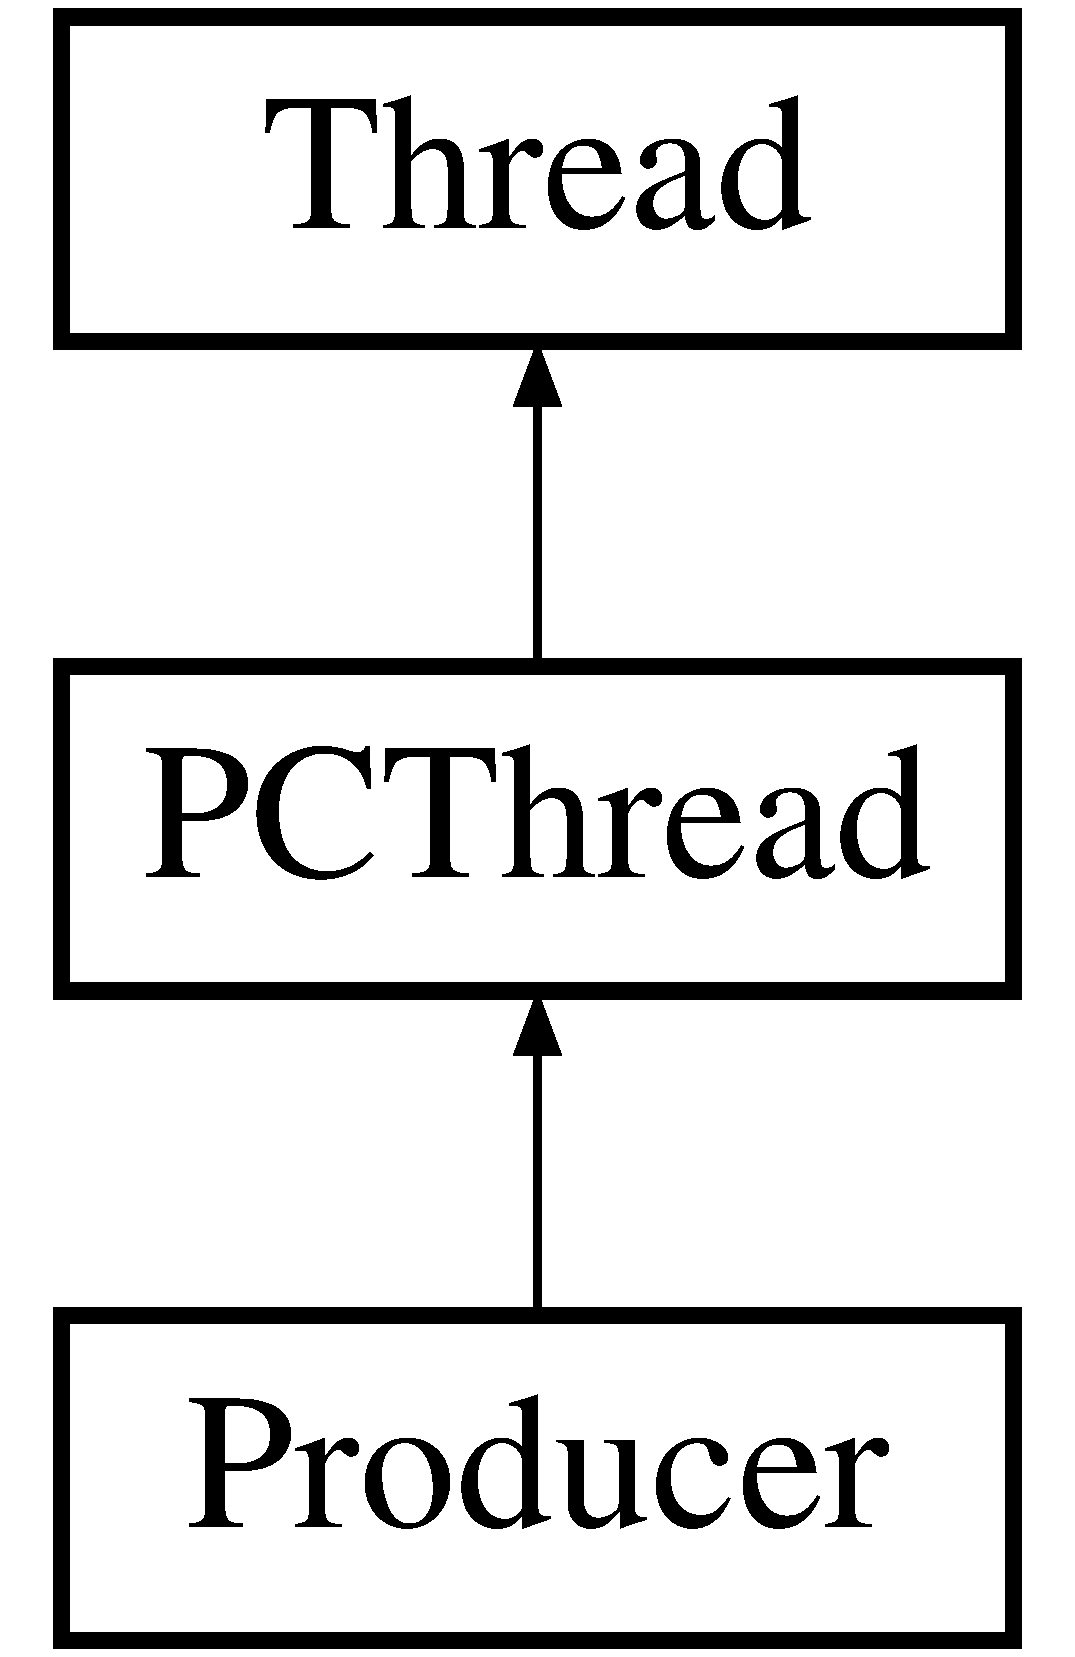
\includegraphics[height=3.000000cm]{class_producer}
\end{center}
\end{figure}
\subsection*{Public Member Functions}
\begin{DoxyCompactItemize}
\item 
\hyperlink{class_producer_ab79ff8b19e682d144e40044485cb81b8}{Producer} ()
\item 
\hyperlink{class_producer_abfb6f8afcc08bdd27e6451c8ae5b0129}{Producer} (\hyperlink{class_queue}{Queue}$<$ \hyperlink{classtsgl_1_1_star}{Star} $\ast$$>$ \&shared\+Buffer, unsigned long id, \hyperlink{classtsgl_1_1_canvas}{Canvas} \&can)
\item 
void \hyperlink{class_producer_ac669b046bc8254d43b7ccc4e3e7a1a8b}{wait} ()
\item 
void \hyperlink{class_producer_aba582d5889728f3d4eb6399a5788ab9f}{lock} ()
\item 
void \hyperlink{class_producer_a40820fecb39439fac7a4f7b4227d4d1d}{act} ()
\item 
void \hyperlink{class_producer_a9a3ce835478573c67a6c8d928ccbf8f0}{unlock} ()
\end{DoxyCompactItemize}
\subsection*{Additional Inherited Members}


\subsection{Detailed Description}
\hyperlink{class_producer}{Producer} class creates a \hyperlink{class_producer}{Producer} object and inherits from the \hyperlink{class_thread}{Thread} class. Inheritance\+: \hyperlink{class_thread}{Thread} class. Implements the abstract run() method from the \hyperlink{class_thread}{Thread} class so that the pthread runs the produce() method. 

\subsection{Constructor \& Destructor Documentation}
\mbox{\Hypertarget{class_producer_ab79ff8b19e682d144e40044485cb81b8}\label{class_producer_ab79ff8b19e682d144e40044485cb81b8}} 
\index{Producer@{Producer}!Producer@{Producer}}
\index{Producer@{Producer}!Producer@{Producer}}
\subsubsection{\texorpdfstring{Producer()}{Producer()}\hspace{0.1cm}{\footnotesize\ttfamily [1/2]}}
{\footnotesize\ttfamily Producer\+::\+Producer (\begin{DoxyParamCaption}{ }\end{DoxyParamCaption})}

Default-\/constructor for the \hyperlink{class_producer}{Producer} class. \begin{DoxyReturn}{Returns}
\+: The constructed \hyperlink{class_producer}{Producer} object. 
\end{DoxyReturn}
\mbox{\Hypertarget{class_producer_abfb6f8afcc08bdd27e6451c8ae5b0129}\label{class_producer_abfb6f8afcc08bdd27e6451c8ae5b0129}} 
\index{Producer@{Producer}!Producer@{Producer}}
\index{Producer@{Producer}!Producer@{Producer}}
\subsubsection{\texorpdfstring{Producer()}{Producer()}\hspace{0.1cm}{\footnotesize\ttfamily [2/2]}}
{\footnotesize\ttfamily Producer\+::\+Producer (\begin{DoxyParamCaption}\item[{\hyperlink{class_queue}{Queue}$<$ \hyperlink{classtsgl_1_1_star}{Star} $\ast$$>$ \&}]{shared\+Buffer,  }\item[{unsigned long}]{id,  }\item[{\hyperlink{classtsgl_1_1_canvas}{Canvas} \&}]{can }\end{DoxyParamCaption})}

Explicit-\/constructor for the \hyperlink{class_producer}{Producer} class. 
\begin{DoxyParams}{Parameters}
{\em } & \\
\hline
\end{DoxyParams}


\subsection{Member Function Documentation}
\mbox{\Hypertarget{class_producer_a40820fecb39439fac7a4f7b4227d4d1d}\label{class_producer_a40820fecb39439fac7a4f7b4227d4d1d}} 
\index{Producer@{Producer}!act@{act}}
\index{act@{act}!Producer@{Producer}}
\subsubsection{\texorpdfstring{act()}{act()}}
{\footnotesize\ttfamily void Producer\+::act (\begin{DoxyParamCaption}{ }\end{DoxyParamCaption})\hspace{0.3cm}{\ttfamily [virtual]}}

act goes through the process of adding a produced item to \hyperlink{class_queue}{Queue} 

Implements \hyperlink{class_p_c_thread}{P\+C\+Thread}.

\mbox{\Hypertarget{class_producer_aba582d5889728f3d4eb6399a5788ab9f}\label{class_producer_aba582d5889728f3d4eb6399a5788ab9f}} 
\index{Producer@{Producer}!lock@{lock}}
\index{lock@{lock}!Producer@{Producer}}
\subsubsection{\texorpdfstring{lock()}{lock()}}
{\footnotesize\ttfamily void Producer\+::lock (\begin{DoxyParamCaption}{ }\end{DoxyParamCaption})\hspace{0.3cm}{\ttfamily [virtual]}}

locks the \hyperlink{class_queue}{Queue} for production 

Implements \hyperlink{class_p_c_thread}{P\+C\+Thread}.

\mbox{\Hypertarget{class_producer_a9a3ce835478573c67a6c8d928ccbf8f0}\label{class_producer_a9a3ce835478573c67a6c8d928ccbf8f0}} 
\index{Producer@{Producer}!unlock@{unlock}}
\index{unlock@{unlock}!Producer@{Producer}}
\subsubsection{\texorpdfstring{unlock()}{unlock()}}
{\footnotesize\ttfamily void Producer\+::unlock (\begin{DoxyParamCaption}{ }\end{DoxyParamCaption})\hspace{0.3cm}{\ttfamily [virtual]}}

unlocks the \hyperlink{class_queue}{Queue} after production 

Implements \hyperlink{class_p_c_thread}{P\+C\+Thread}.

\mbox{\Hypertarget{class_producer_ac669b046bc8254d43b7ccc4e3e7a1a8b}\label{class_producer_ac669b046bc8254d43b7ccc4e3e7a1a8b}} 
\index{Producer@{Producer}!wait@{wait}}
\index{wait@{wait}!Producer@{Producer}}
\subsubsection{\texorpdfstring{wait()}{wait()}}
{\footnotesize\ttfamily void Producer\+::wait (\begin{DoxyParamCaption}{ }\end{DoxyParamCaption})\hspace{0.3cm}{\ttfamily [virtual]}}

wait takes some time to find the next color 

Reimplemented from \hyperlink{class_p_c_thread}{P\+C\+Thread}.



The documentation for this class was generated from the following files\+:\begin{DoxyCompactItemize}
\item 
/home/sth5/test/\+T\+S\+G\+L/src/examples/\+Producer\+Consumer/Producer.\+h\item 
/home/sth5/test/\+T\+S\+G\+L/src/examples/\+Producer\+Consumer/Producer.\+cpp\end{DoxyCompactItemize}

\hypertarget{classtsgl_1_1_progress_bar}{}\section{tsgl\+:\+:Progress\+Bar Class Reference}
\label{classtsgl_1_1_progress_bar}\index{tsgl\+::\+Progress\+Bar@{tsgl\+::\+Progress\+Bar}}


Draws and updates a progress bar.  




{\ttfamily \#include $<$Progress\+Bar.\+h$>$}

\subsection*{Public Member Functions}
\begin{DoxyCompactItemize}
\item 
\hyperlink{classtsgl_1_1_progress_bar_ac79018d09a75c490de3490306146c010}{Progress\+Bar} (int x, int y, int width, int height, float min\+Value, float max\+Value, unsigned num\+Segments)
\begin{DoxyCompactList}\small\item\em Explicit \hyperlink{classtsgl_1_1_progress_bar}{Progress\+Bar} constructor method. \end{DoxyCompactList}\item 
\hyperlink{classtsgl_1_1_progress_bar_aa3ad600db2cbd0e8f9221c264535df21}{$\sim$\+Progress\+Bar} ()
\begin{DoxyCompactList}\small\item\em \hyperlink{classtsgl_1_1_progress_bar}{Progress\+Bar} destructor method. \end{DoxyCompactList}\item 
void \hyperlink{classtsgl_1_1_progress_bar_a4274998e4935f33eb9212b2174d9c0c5}{update} (float new\+Value, int segnum=-\/1)
\begin{DoxyCompactList}\small\item\em Updates a \hyperlink{classtsgl_1_1_progress_bar}{Progress\+Bar} segment with a new value. \end{DoxyCompactList}\item 
\hyperlink{classtsgl_1_1_polyline}{Polyline} $\ast$ \hyperlink{classtsgl_1_1_progress_bar_ac2b51bdb0d19afaa03d60a9928fc873f}{get\+Border} (int index)
\begin{DoxyCompactList}\small\item\em Accessor for the \hyperlink{classtsgl_1_1_progress_bar}{Progress\+Bar}\textquotesingle{}s representative \hyperlink{classtsgl_1_1_polyline}{Polyline} array. \end{DoxyCompactList}\item 
\hyperlink{classtsgl_1_1_rectangle}{Rectangle} $\ast$ \hyperlink{classtsgl_1_1_progress_bar_aa360099f70e0c33c99f349cf28cbe610}{get\+Rect} (int index)
\begin{DoxyCompactList}\small\item\em Accessor for the \hyperlink{classtsgl_1_1_progress_bar}{Progress\+Bar}\textquotesingle{}s representative \hyperlink{classtsgl_1_1_rectangle}{Rectangle} array. \end{DoxyCompactList}\item 
int \hyperlink{classtsgl_1_1_progress_bar_a25576903783f18f8d74570aed2f80d95}{get\+Segs} ()
\begin{DoxyCompactList}\small\item\em Accessor for the \hyperlink{classtsgl_1_1_progress_bar}{Progress\+Bar}\textquotesingle{}s number of segments. \end{DoxyCompactList}\item 
int \hyperlink{classtsgl_1_1_progress_bar_a7ecdc35e44496db7cf2e25b2ee6577d4}{get\+Seg\+X} (int i)
\begin{DoxyCompactList}\small\item\em Accessor for a segment\textquotesingle{}s x position. \end{DoxyCompactList}\item 
int \hyperlink{classtsgl_1_1_progress_bar_a7efb6be08196ad2b48d4417a93d750ad}{get\+Seg\+Y} ()
\begin{DoxyCompactList}\small\item\em Accessor for a segment\textquotesingle{}s y position. \end{DoxyCompactList}\end{DoxyCompactItemize}


\subsection{Detailed Description}
Draws and updates a progress bar. 

\hyperlink{classtsgl_1_1_progress_bar}{Progress\+Bar} is a class for holding vertex data for multiple rectangles forming a progress bar. \hyperlink{classtsgl_1_1_progress_bar}{Progress\+Bar} is formed of multiple segments, each of which is thread-\/safe and updated individually with the \hyperlink{classtsgl_1_1_progress_bar_a4274998e4935f33eb9212b2174d9c0c5}{update()} method. A \hyperlink{classtsgl_1_1_progress_bar}{Progress\+Bar} can be drawn to the screen using \hyperlink{classtsgl_1_1_canvas_aea792059486ebe6d25d7f81bdadf751d}{Canvas\+::draw\+Progress()}. 

\subsection{Constructor \& Destructor Documentation}
\hypertarget{classtsgl_1_1_progress_bar_ac79018d09a75c490de3490306146c010}{}\index{tsgl\+::\+Progress\+Bar@{tsgl\+::\+Progress\+Bar}!Progress\+Bar@{Progress\+Bar}}
\index{Progress\+Bar@{Progress\+Bar}!tsgl\+::\+Progress\+Bar@{tsgl\+::\+Progress\+Bar}}
\subsubsection[{Progress\+Bar}]{\setlength{\rightskip}{0pt plus 5cm}tsgl\+::\+Progress\+Bar\+::\+Progress\+Bar (
\begin{DoxyParamCaption}
\item[{int}]{x, }
\item[{int}]{y, }
\item[{int}]{width, }
\item[{int}]{height, }
\item[{float}]{min\+Value, }
\item[{float}]{max\+Value, }
\item[{unsigned}]{num\+Segments}
\end{DoxyParamCaption}
)}\label{classtsgl_1_1_progress_bar_ac79018d09a75c490de3490306146c010}


Explicit \hyperlink{classtsgl_1_1_progress_bar}{Progress\+Bar} constructor method. 

This is the explicit constructor for the \hyperlink{classtsgl_1_1_progress_bar}{Progress\+Bar} class. 
\begin{DoxyParams}{Parameters}
{\em x} & The x position of the left edge of the \hyperlink{classtsgl_1_1_progress_bar}{Progress\+Bar}. \\
\hline
{\em y} & The y position of the top edge of the \hyperlink{classtsgl_1_1_progress_bar}{Progress\+Bar}. \\
\hline
{\em width} & The maximum width in pixels of the \hyperlink{classtsgl_1_1_progress_bar}{Progress\+Bar}. \\
\hline
{\em height} & The maximum height in pixels of the \hyperlink{classtsgl_1_1_progress_bar}{Progress\+Bar}. \\
\hline
{\em min\+Value} & The minimum value represented by the \hyperlink{classtsgl_1_1_progress_bar}{Progress\+Bar}. \\
\hline
{\em max\+Value} & The maximum value represented by the \hyperlink{classtsgl_1_1_progress_bar}{Progress\+Bar}. \\
\hline
{\em num\+Segments} & The number of segments in the progress bar \\
\hline
\end{DoxyParams}
\begin{DoxyReturn}{Returns}
A new \hyperlink{classtsgl_1_1_progress_bar}{Progress\+Bar} with the specified coordinates, maximum dimensions, value range, and segments. 
\end{DoxyReturn}
\hypertarget{classtsgl_1_1_progress_bar_aa3ad600db2cbd0e8f9221c264535df21}{}\index{tsgl\+::\+Progress\+Bar@{tsgl\+::\+Progress\+Bar}!````~Progress\+Bar@{$\sim$\+Progress\+Bar}}
\index{````~Progress\+Bar@{$\sim$\+Progress\+Bar}!tsgl\+::\+Progress\+Bar@{tsgl\+::\+Progress\+Bar}}
\subsubsection[{$\sim$\+Progress\+Bar}]{\setlength{\rightskip}{0pt plus 5cm}tsgl\+::\+Progress\+Bar\+::$\sim$\+Progress\+Bar (
\begin{DoxyParamCaption}
{}
\end{DoxyParamCaption}
)}\label{classtsgl_1_1_progress_bar_aa3ad600db2cbd0e8f9221c264535df21}


\hyperlink{classtsgl_1_1_progress_bar}{Progress\+Bar} destructor method. 

This is the destructor for the \hyperlink{classtsgl_1_1_progress_bar}{Progress\+Bar} class.

Frees up memory that was allocated to a \hyperlink{classtsgl_1_1_progress_bar}{Progress\+Bar} instance. 

\subsection{Member Function Documentation}
\hypertarget{classtsgl_1_1_progress_bar_ac2b51bdb0d19afaa03d60a9928fc873f}{}\index{tsgl\+::\+Progress\+Bar@{tsgl\+::\+Progress\+Bar}!get\+Border@{get\+Border}}
\index{get\+Border@{get\+Border}!tsgl\+::\+Progress\+Bar@{tsgl\+::\+Progress\+Bar}}
\subsubsection[{get\+Border}]{\setlength{\rightskip}{0pt plus 5cm}{\bf Polyline} $\ast$ tsgl\+::\+Progress\+Bar\+::get\+Border (
\begin{DoxyParamCaption}
\item[{int}]{index}
\end{DoxyParamCaption}
)}\label{classtsgl_1_1_progress_bar_ac2b51bdb0d19afaa03d60a9928fc873f}


Accessor for the \hyperlink{classtsgl_1_1_progress_bar}{Progress\+Bar}\textquotesingle{}s representative \hyperlink{classtsgl_1_1_polyline}{Polyline} array. 


\begin{DoxyParams}{Parameters}
{\em index} & Index of the segment to access. \\
\hline
\end{DoxyParams}
\begin{DoxyReturn}{Returns}
A pointer to the \hyperlink{classtsgl_1_1_polyline}{Polyline} array representing segment border {\ttfamily i} of the \hyperlink{classtsgl_1_1_progress_bar}{Progress\+Bar}. 
\end{DoxyReturn}


Referenced by tsgl\+::\+Canvas\+::draw\+Progress().

\hypertarget{classtsgl_1_1_progress_bar_aa360099f70e0c33c99f349cf28cbe610}{}\index{tsgl\+::\+Progress\+Bar@{tsgl\+::\+Progress\+Bar}!get\+Rect@{get\+Rect}}
\index{get\+Rect@{get\+Rect}!tsgl\+::\+Progress\+Bar@{tsgl\+::\+Progress\+Bar}}
\subsubsection[{get\+Rect}]{\setlength{\rightskip}{0pt plus 5cm}{\bf Rectangle} $\ast$ tsgl\+::\+Progress\+Bar\+::get\+Rect (
\begin{DoxyParamCaption}
\item[{int}]{index}
\end{DoxyParamCaption}
)}\label{classtsgl_1_1_progress_bar_aa360099f70e0c33c99f349cf28cbe610}


Accessor for the \hyperlink{classtsgl_1_1_progress_bar}{Progress\+Bar}\textquotesingle{}s representative \hyperlink{classtsgl_1_1_rectangle}{Rectangle} array. 


\begin{DoxyParams}{Parameters}
{\em index} & Index of the segment to access. \\
\hline
\end{DoxyParams}
\begin{DoxyReturn}{Returns}
A pointer to the \hyperlink{classtsgl_1_1_rectangle}{Rectangle} array representing segment {\ttfamily i} of the \hyperlink{classtsgl_1_1_progress_bar}{Progress\+Bar}. 
\end{DoxyReturn}


Referenced by tsgl\+::\+Canvas\+::draw\+Progress().

\hypertarget{classtsgl_1_1_progress_bar_a25576903783f18f8d74570aed2f80d95}{}\index{tsgl\+::\+Progress\+Bar@{tsgl\+::\+Progress\+Bar}!get\+Segs@{get\+Segs}}
\index{get\+Segs@{get\+Segs}!tsgl\+::\+Progress\+Bar@{tsgl\+::\+Progress\+Bar}}
\subsubsection[{get\+Segs}]{\setlength{\rightskip}{0pt plus 5cm}int tsgl\+::\+Progress\+Bar\+::get\+Segs (
\begin{DoxyParamCaption}
{}
\end{DoxyParamCaption}
)\hspace{0.3cm}{\ttfamily [inline]}}\label{classtsgl_1_1_progress_bar_a25576903783f18f8d74570aed2f80d95}


Accessor for the \hyperlink{classtsgl_1_1_progress_bar}{Progress\+Bar}\textquotesingle{}s number of segments. 

\begin{DoxyReturn}{Returns}
The number of segments in the \hyperlink{classtsgl_1_1_progress_bar}{Progress\+Bar}. 
\end{DoxyReturn}


Referenced by tsgl\+::\+Canvas\+::draw\+Progress().

\hypertarget{classtsgl_1_1_progress_bar_a7ecdc35e44496db7cf2e25b2ee6577d4}{}\index{tsgl\+::\+Progress\+Bar@{tsgl\+::\+Progress\+Bar}!get\+Seg\+X@{get\+Seg\+X}}
\index{get\+Seg\+X@{get\+Seg\+X}!tsgl\+::\+Progress\+Bar@{tsgl\+::\+Progress\+Bar}}
\subsubsection[{get\+Seg\+X}]{\setlength{\rightskip}{0pt plus 5cm}int tsgl\+::\+Progress\+Bar\+::get\+Seg\+X (
\begin{DoxyParamCaption}
\item[{int}]{i}
\end{DoxyParamCaption}
)\hspace{0.3cm}{\ttfamily [inline]}}\label{classtsgl_1_1_progress_bar_a7ecdc35e44496db7cf2e25b2ee6577d4}


Accessor for a segment\textquotesingle{}s x position. 


\begin{DoxyParams}{Parameters}
{\em i} & Index of the segment \\
\hline
\end{DoxyParams}
\begin{DoxyReturn}{Returns}
The x-\/coordinate of the left edge of segment {\ttfamily i} in the \hyperlink{classtsgl_1_1_progress_bar}{Progress\+Bar}. 
\end{DoxyReturn}


Referenced by tsgl\+::\+Canvas\+::draw\+Progress().

\hypertarget{classtsgl_1_1_progress_bar_a7efb6be08196ad2b48d4417a93d750ad}{}\index{tsgl\+::\+Progress\+Bar@{tsgl\+::\+Progress\+Bar}!get\+Seg\+Y@{get\+Seg\+Y}}
\index{get\+Seg\+Y@{get\+Seg\+Y}!tsgl\+::\+Progress\+Bar@{tsgl\+::\+Progress\+Bar}}
\subsubsection[{get\+Seg\+Y}]{\setlength{\rightskip}{0pt plus 5cm}int tsgl\+::\+Progress\+Bar\+::get\+Seg\+Y (
\begin{DoxyParamCaption}
{}
\end{DoxyParamCaption}
)\hspace{0.3cm}{\ttfamily [inline]}}\label{classtsgl_1_1_progress_bar_a7efb6be08196ad2b48d4417a93d750ad}


Accessor for a segment\textquotesingle{}s y position. 

\begin{DoxyReturn}{Returns}
The y-\/coordinate of the top edge of the \hyperlink{classtsgl_1_1_progress_bar}{Progress\+Bar}. 
\end{DoxyReturn}


Referenced by tsgl\+::\+Canvas\+::draw\+Progress().

\hypertarget{classtsgl_1_1_progress_bar_a4274998e4935f33eb9212b2174d9c0c5}{}\index{tsgl\+::\+Progress\+Bar@{tsgl\+::\+Progress\+Bar}!update@{update}}
\index{update@{update}!tsgl\+::\+Progress\+Bar@{tsgl\+::\+Progress\+Bar}}
\subsubsection[{update}]{\setlength{\rightskip}{0pt plus 5cm}void tsgl\+::\+Progress\+Bar\+::update (
\begin{DoxyParamCaption}
\item[{float}]{new\+Value, }
\item[{int}]{segnum = {\ttfamily -\/1}}
\end{DoxyParamCaption}
)}\label{classtsgl_1_1_progress_bar_a4274998e4935f33eb9212b2174d9c0c5}


Updates a \hyperlink{classtsgl_1_1_progress_bar}{Progress\+Bar} segment with a new value. 

This function updates the segment {\ttfamily seg} of the \hyperlink{classtsgl_1_1_progress_bar}{Progress\+Bar} to represent the new value {\ttfamily new\+V}. If new\+V is less than the segment\textquotesingle{}s minimum value, the segment is set to its minimum value. If new\+V is more than the segment\textquotesingle{}s maximum value, the segment is set to its maximum value. 
\begin{DoxyParams}{Parameters}
{\em new\+Value} & The value to set the segment to. \\
\hline
{\em segnum} & The segment whose value to update. A value of -\/1 indicates the current thread number. \\
\hline
\end{DoxyParams}
\begin{DoxyNote}{Note}
The minimum value for a segment is calculated as {\ttfamily min\+V + (max\+V-\/min\+V)$\ast$seg/segs} 

The maximum value for a segment is calculated as {\ttfamily min\+V + (max\+V-\/min\+V)$\ast$(seg+1)/segs} 
\end{DoxyNote}


The documentation for this class was generated from the following files\+:\begin{DoxyCompactItemize}
\item 
Progress\+Bar.\+h\item 
Progress\+Bar.\+cpp\end{DoxyCompactItemize}

\hypertarget{classtsgl_1_1_pyramid}{}\section{tsgl\+:\+:Pyramid Class Reference}
\label{classtsgl_1_1_pyramid}\index{tsgl\+::\+Pyramid@{tsgl\+::\+Pyramid}}


Draw an arbitrary \hyperlink{classtsgl_1_1_pyramid}{Pyramid} with colored vertices.  




{\ttfamily \#include $<$Pyramid.\+h$>$}

Inheritance diagram for tsgl\+:\+:Pyramid\+:\begin{figure}[H]
\begin{center}
\leavevmode
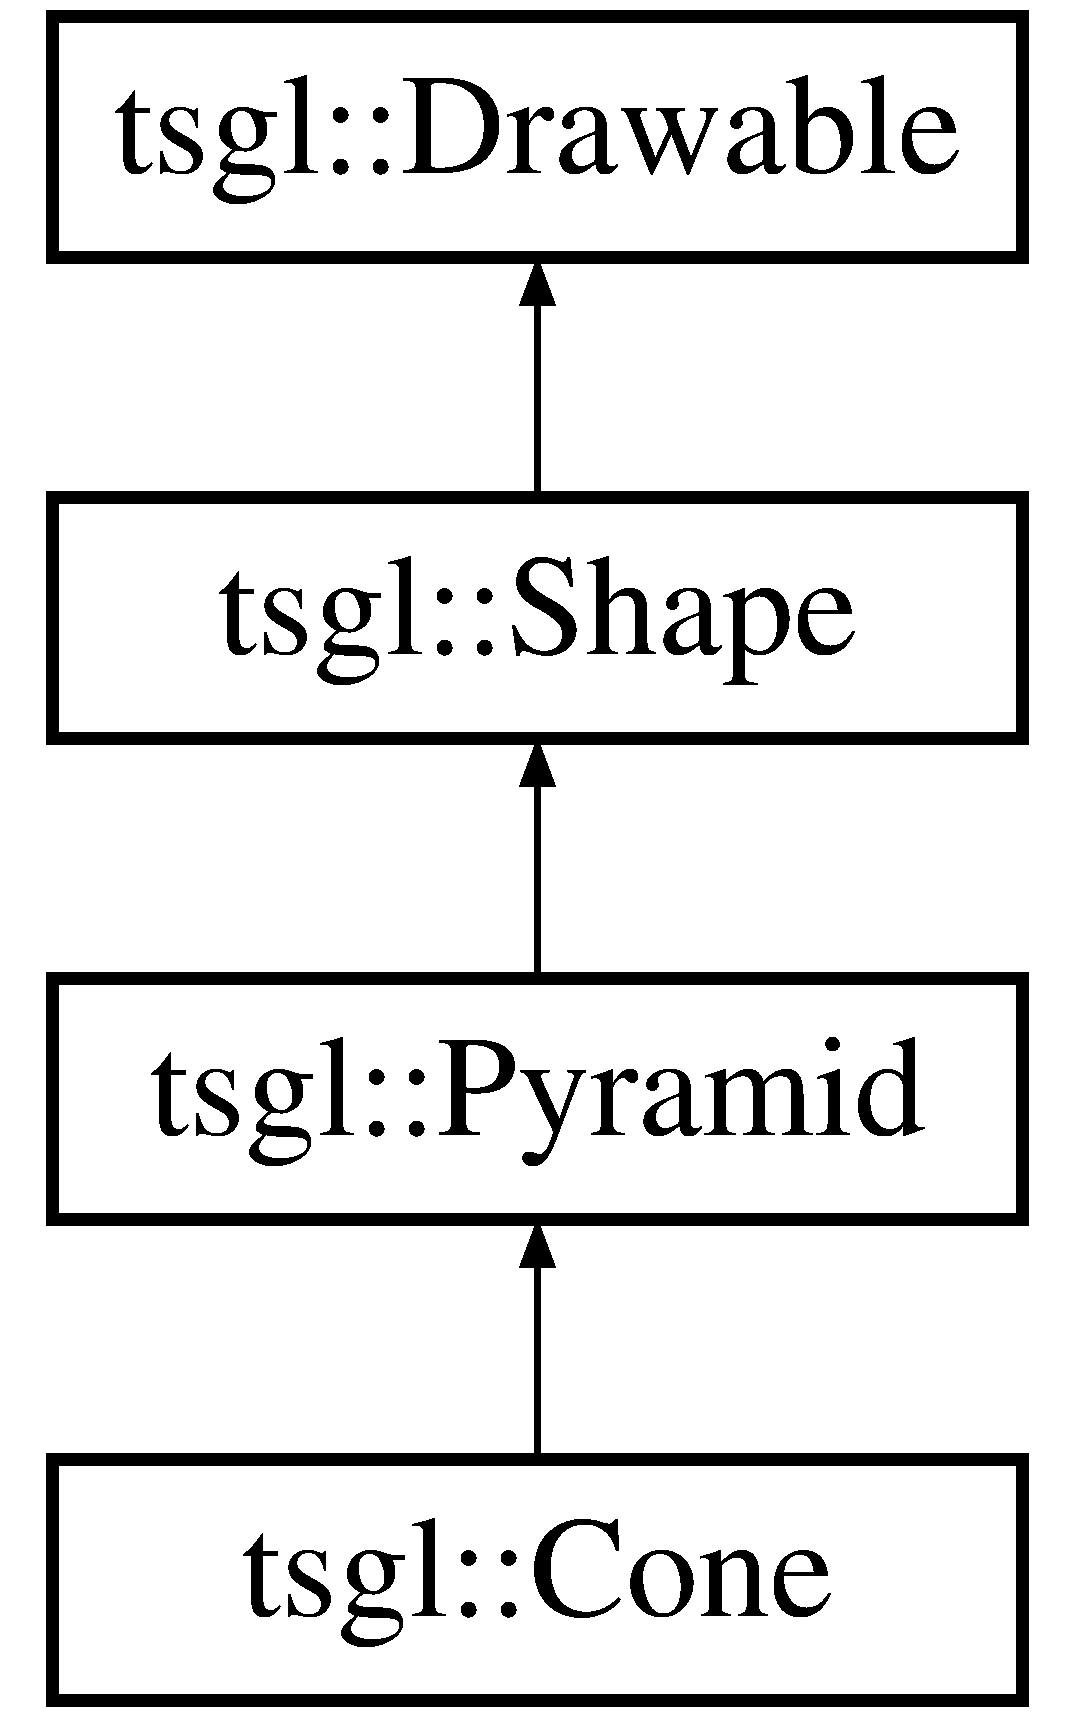
\includegraphics[height=4.000000cm]{classtsgl_1_1_pyramid}
\end{center}
\end{figure}
\subsection*{Public Member Functions}
\begin{DoxyCompactItemize}
\item 
\hyperlink{classtsgl_1_1_pyramid_ad980b2565031617f41a89d62a85f4c85}{Pyramid} (float x, float y, float z, int sides, G\+Lfloat height, G\+Lfloat radius, float yaw, float pitch, float roll, \hyperlink{structtsgl_1_1_color_float}{Color\+Float} c)
\begin{DoxyCompactList}\small\item\em Explicitly constructs a new \hyperlink{classtsgl_1_1_pyramid}{Pyramid}. \end{DoxyCompactList}\item 
\hyperlink{classtsgl_1_1_pyramid_aeefc2de2b046398e194fc8b041eedc95}{Pyramid} (float x, float y, float z, int sides, G\+Lfloat height, G\+Lfloat radius, float yaw, float pitch, float roll, \hyperlink{structtsgl_1_1_color_float}{Color\+Float} c\mbox{[}$\,$\mbox{]})
\begin{DoxyCompactList}\small\item\em Explicitly constructs a new \hyperlink{classtsgl_1_1_pyramid}{Pyramid}. \end{DoxyCompactList}\item 
virtual void \hyperlink{classtsgl_1_1_pyramid_ac949cacc0db5fb112d92e2ec987cd5c3}{set\+Radius} (float radius)
\begin{DoxyCompactList}\small\item\em Mutates the \hyperlink{classtsgl_1_1_pyramid}{Pyramid}\textquotesingle{}s base\textquotesingle{}s radius. \end{DoxyCompactList}\item 
virtual void \hyperlink{classtsgl_1_1_pyramid_a91f86ca2ac58df9ac8d2ad00781b8442}{change\+Radius\+By} (float delta)
\begin{DoxyCompactList}\small\item\em Mutates the \hyperlink{classtsgl_1_1_pyramid}{Pyramid}\textquotesingle{}s base\textquotesingle{}s radius by the parameter amount. \end{DoxyCompactList}\item 
virtual void \hyperlink{classtsgl_1_1_pyramid_acb4db4a56452bb0e45dcd120ef517747}{set\+Height} (float height)
\begin{DoxyCompactList}\small\item\em Mutates the distance from the center of the \hyperlink{classtsgl_1_1_pyramid}{Pyramid}\textquotesingle{}s base to the tip. \end{DoxyCompactList}\item 
virtual void \hyperlink{classtsgl_1_1_pyramid_af7a7b6f5a83b9f6b59a9c6ae0c6812d9}{change\+Height\+By} (float delta)
\begin{DoxyCompactList}\small\item\em Mutates the distance from the center of the \hyperlink{classtsgl_1_1_pyramid}{Pyramid}\textquotesingle{}s base to the tip by the parameter amount. \end{DoxyCompactList}\item 
virtual G\+Lfloat \hyperlink{classtsgl_1_1_pyramid_a4511f7d6a89b061a83dc0fda00ff0c31}{get\+Height} ()
\begin{DoxyCompactList}\small\item\em Accessor for the height of the \hyperlink{classtsgl_1_1_prism}{Prism}. \end{DoxyCompactList}\item 
virtual G\+Lfloat \hyperlink{classtsgl_1_1_pyramid_a778d993a925720d1db6edb17f92dd381}{get\+Radius} ()
\begin{DoxyCompactList}\small\item\em Accessor for the radius of the \hyperlink{classtsgl_1_1_prism}{Prism}. \end{DoxyCompactList}\item 
virtual void \hyperlink{classtsgl_1_1_pyramid_aef16d8830e2dfac0e8a30d091d099c30}{set\+Color} (\hyperlink{structtsgl_1_1_color_float}{Color\+Float} c)
\begin{DoxyCompactList}\small\item\em Sets the \hyperlink{classtsgl_1_1_pyramid}{Pyramid} to a new color. \end{DoxyCompactList}\item 
virtual void \hyperlink{classtsgl_1_1_pyramid_a83799687df3bdef698f9687da7a6c100}{set\+Color} (\hyperlink{structtsgl_1_1_color_float}{Color\+Float} c\mbox{[}$\,$\mbox{]})
\begin{DoxyCompactList}\small\item\em Sets the \hyperlink{classtsgl_1_1_pyramid}{Pyramid} to an array of new colors. \end{DoxyCompactList}\item 
virtual void \hyperlink{classtsgl_1_1_pyramid_a9c93002e90ac1f3385c4d3154ca0321a}{get\+Colors} (std\+::vector$<$ \hyperlink{structtsgl_1_1_color_float}{Color\+Float} $>$ \&color\+Vec)
\begin{DoxyCompactList}\small\item\em Accessor for \hyperlink{classtsgl_1_1_arrow}{Arrow}\textquotesingle{}s colors. \end{DoxyCompactList}\end{DoxyCompactItemize}
\subsection*{Protected Attributes}
\begin{DoxyCompactItemize}
\item 
\mbox{\Hypertarget{classtsgl_1_1_pyramid_ae413ddfe4c3adb247b046c6322c569da}\label{classtsgl_1_1_pyramid_ae413ddfe4c3adb247b046c6322c569da}} 
G\+Lfloat {\bfseries my\+Height}
\item 
\mbox{\Hypertarget{classtsgl_1_1_pyramid_a290d3c2312d62f4573e4bd6aff3a8b00}\label{classtsgl_1_1_pyramid_a290d3c2312d62f4573e4bd6aff3a8b00}} 
G\+Lfloat {\bfseries my\+Radius}
\item 
\mbox{\Hypertarget{classtsgl_1_1_pyramid_a5c4f2b3063e23ae0492b6e00e8d9100a}\label{classtsgl_1_1_pyramid_a5c4f2b3063e23ae0492b6e00e8d9100a}} 
int {\bfseries my\+Sides}
\end{DoxyCompactItemize}
\subsection*{Additional Inherited Members}


\subsection{Detailed Description}
Draw an arbitrary \hyperlink{classtsgl_1_1_pyramid}{Pyramid} with colored vertices. 

\hyperlink{classtsgl_1_1_pyramid}{Pyramid} is a class for holding vertex data for a pyramid with a base with at least 3 sides. 

\subsection{Constructor \& Destructor Documentation}
\mbox{\Hypertarget{classtsgl_1_1_pyramid_ad980b2565031617f41a89d62a85f4c85}\label{classtsgl_1_1_pyramid_ad980b2565031617f41a89d62a85f4c85}} 
\index{tsgl\+::\+Pyramid@{tsgl\+::\+Pyramid}!Pyramid@{Pyramid}}
\index{Pyramid@{Pyramid}!tsgl\+::\+Pyramid@{tsgl\+::\+Pyramid}}
\subsubsection{\texorpdfstring{Pyramid()}{Pyramid()}\hspace{0.1cm}{\footnotesize\ttfamily [1/2]}}
{\footnotesize\ttfamily tsgl\+::\+Pyramid\+::\+Pyramid (\begin{DoxyParamCaption}\item[{float}]{x,  }\item[{float}]{y,  }\item[{float}]{z,  }\item[{int}]{sides,  }\item[{G\+Lfloat}]{height,  }\item[{G\+Lfloat}]{radius,  }\item[{float}]{yaw,  }\item[{float}]{pitch,  }\item[{float}]{roll,  }\item[{\hyperlink{structtsgl_1_1_color_float}{Color\+Float}}]{c }\end{DoxyParamCaption})}



Explicitly constructs a new \hyperlink{classtsgl_1_1_pyramid}{Pyramid}. 

Explicit constructor for a \hyperlink{classtsgl_1_1_pyramid}{Pyramid} object. 
\begin{DoxyParams}{Parameters}
{\em x} & The x coordinate of the center of the \hyperlink{classtsgl_1_1_pyramid}{Pyramid}. \\
\hline
{\em y} & The y coordinate of the center of the \hyperlink{classtsgl_1_1_pyramid}{Pyramid}. \\
\hline
{\em z} & The z coordinate of the center of the \hyperlink{classtsgl_1_1_pyramid}{Pyramid}. \\
\hline
{\em height} & The distance from the center of the base to tip of the \hyperlink{classtsgl_1_1_pyramid}{Pyramid}. \\
\hline
{\em radius} & The distance from the center of the \hyperlink{classtsgl_1_1_pyramid}{Pyramid}\textquotesingle{}s base to each vertex of the base. \\
\hline
{\em sides} & The number of sides of the \hyperlink{classtsgl_1_1_pyramid}{Pyramid}\textquotesingle{}s base. \\
\hline
{\em yaw} & The \hyperlink{classtsgl_1_1_pyramid}{Pyramid}\textquotesingle{}s yaw. \\
\hline
{\em pitch} & The \hyperlink{classtsgl_1_1_pyramid}{Pyramid}\textquotesingle{}s pitch. \\
\hline
{\em roll} & The \hyperlink{classtsgl_1_1_pyramid}{Pyramid}\textquotesingle{}s roll. \\
\hline
{\em c} & A \hyperlink{structtsgl_1_1_color_float}{Color\+Float} for the \hyperlink{classtsgl_1_1_pyramid}{Pyramid}\textquotesingle{}s vertex colors. \\
\hline
\end{DoxyParams}
\begin{DoxyWarning}{Warning}
An invariant is held where if sides is less than 3 then an error message is given. 

An invariant is held where if radius isn\textquotesingle{}t positive then an error message is given. 
\end{DoxyWarning}
\begin{DoxyReturn}{Returns}
A new \hyperlink{classtsgl_1_1_pyramid}{Pyramid} with a buffer for storing the specified numbered of vertices. 
\end{DoxyReturn}
\mbox{\Hypertarget{classtsgl_1_1_pyramid_aeefc2de2b046398e194fc8b041eedc95}\label{classtsgl_1_1_pyramid_aeefc2de2b046398e194fc8b041eedc95}} 
\index{tsgl\+::\+Pyramid@{tsgl\+::\+Pyramid}!Pyramid@{Pyramid}}
\index{Pyramid@{Pyramid}!tsgl\+::\+Pyramid@{tsgl\+::\+Pyramid}}
\subsubsection{\texorpdfstring{Pyramid()}{Pyramid()}\hspace{0.1cm}{\footnotesize\ttfamily [2/2]}}
{\footnotesize\ttfamily tsgl\+::\+Pyramid\+::\+Pyramid (\begin{DoxyParamCaption}\item[{float}]{x,  }\item[{float}]{y,  }\item[{float}]{z,  }\item[{int}]{sides,  }\item[{G\+Lfloat}]{height,  }\item[{G\+Lfloat}]{radius,  }\item[{float}]{yaw,  }\item[{float}]{pitch,  }\item[{float}]{roll,  }\item[{\hyperlink{structtsgl_1_1_color_float}{Color\+Float}}]{c\mbox{[}$\,$\mbox{]} }\end{DoxyParamCaption})}



Explicitly constructs a new \hyperlink{classtsgl_1_1_pyramid}{Pyramid}. 

Explicit constructor for a \hyperlink{classtsgl_1_1_pyramid}{Pyramid} object. 
\begin{DoxyParams}{Parameters}
{\em x} & The x coordinate of the center of the \hyperlink{classtsgl_1_1_pyramid}{Pyramid}. \\
\hline
{\em y} & The y coordinate of the center of the \hyperlink{classtsgl_1_1_pyramid}{Pyramid}. \\
\hline
{\em z} & The z coordinate of the center of the \hyperlink{classtsgl_1_1_pyramid}{Pyramid}. \\
\hline
{\em height} & The distance from the center of the base to tip of the \hyperlink{classtsgl_1_1_pyramid}{Pyramid}. \\
\hline
{\em radius} & The distance from the center of the \hyperlink{classtsgl_1_1_pyramid}{Pyramid}\textquotesingle{}s base to each vertex of the base. \\
\hline
{\em sides} & The number of sides of the \hyperlink{classtsgl_1_1_pyramid}{Pyramid}\textquotesingle{}s base. \\
\hline
{\em yaw} & The \hyperlink{classtsgl_1_1_pyramid}{Pyramid}\textquotesingle{}s yaw. \\
\hline
{\em pitch} & The \hyperlink{classtsgl_1_1_pyramid}{Pyramid}\textquotesingle{}s pitch. \\
\hline
{\em roll} & The \hyperlink{classtsgl_1_1_pyramid}{Pyramid}\textquotesingle{}s roll. \\
\hline
{\em c} & An array of Color\+Floats for the \hyperlink{classtsgl_1_1_pyramid}{Pyramid}\textquotesingle{}s vertex colors. \\
\hline
\end{DoxyParams}
\begin{DoxyWarning}{Warning}
An invariant is held where if sides is less than 3 then an error message is given. 

An invariant is held where if radius isn\textquotesingle{}t positive then an error message is given. 
\end{DoxyWarning}
\begin{DoxyReturn}{Returns}
A new \hyperlink{classtsgl_1_1_pyramid}{Pyramid} with a buffer for storing the specified numbered of vertices. 
\end{DoxyReturn}


\subsection{Member Function Documentation}
\mbox{\Hypertarget{classtsgl_1_1_pyramid_af7a7b6f5a83b9f6b59a9c6ae0c6812d9}\label{classtsgl_1_1_pyramid_af7a7b6f5a83b9f6b59a9c6ae0c6812d9}} 
\index{tsgl\+::\+Pyramid@{tsgl\+::\+Pyramid}!change\+Height\+By@{change\+Height\+By}}
\index{change\+Height\+By@{change\+Height\+By}!tsgl\+::\+Pyramid@{tsgl\+::\+Pyramid}}
\subsubsection{\texorpdfstring{change\+Height\+By()}{changeHeightBy()}}
{\footnotesize\ttfamily void tsgl\+::\+Pyramid\+::change\+Height\+By (\begin{DoxyParamCaption}\item[{float}]{delta }\end{DoxyParamCaption})\hspace{0.3cm}{\ttfamily [virtual]}}



Mutates the distance from the center of the \hyperlink{classtsgl_1_1_pyramid}{Pyramid}\textquotesingle{}s base to the tip by the parameter amount. 


\begin{DoxyParams}{Parameters}
{\em delta} & The amount by which to change the height of the pyramid. \\
\hline
\end{DoxyParams}
\mbox{\Hypertarget{classtsgl_1_1_pyramid_a91f86ca2ac58df9ac8d2ad00781b8442}\label{classtsgl_1_1_pyramid_a91f86ca2ac58df9ac8d2ad00781b8442}} 
\index{tsgl\+::\+Pyramid@{tsgl\+::\+Pyramid}!change\+Radius\+By@{change\+Radius\+By}}
\index{change\+Radius\+By@{change\+Radius\+By}!tsgl\+::\+Pyramid@{tsgl\+::\+Pyramid}}
\subsubsection{\texorpdfstring{change\+Radius\+By()}{changeRadiusBy()}}
{\footnotesize\ttfamily void tsgl\+::\+Pyramid\+::change\+Radius\+By (\begin{DoxyParamCaption}\item[{float}]{delta }\end{DoxyParamCaption})\hspace{0.3cm}{\ttfamily [virtual]}}



Mutates the \hyperlink{classtsgl_1_1_pyramid}{Pyramid}\textquotesingle{}s base\textquotesingle{}s radius by the parameter amount. 


\begin{DoxyParams}{Parameters}
{\em delta} & The amount by which to change the radius of the \hyperlink{classtsgl_1_1_pyramid}{Pyramid}\textquotesingle{}s base. \\
\hline
\end{DoxyParams}
\mbox{\Hypertarget{classtsgl_1_1_pyramid_a9c93002e90ac1f3385c4d3154ca0321a}\label{classtsgl_1_1_pyramid_a9c93002e90ac1f3385c4d3154ca0321a}} 
\index{tsgl\+::\+Pyramid@{tsgl\+::\+Pyramid}!get\+Colors@{get\+Colors}}
\index{get\+Colors@{get\+Colors}!tsgl\+::\+Pyramid@{tsgl\+::\+Pyramid}}
\subsubsection{\texorpdfstring{get\+Colors()}{getColors()}}
{\footnotesize\ttfamily void tsgl\+::\+Pyramid\+::get\+Colors (\begin{DoxyParamCaption}\item[{std\+::vector$<$ \hyperlink{structtsgl_1_1_color_float}{Color\+Float} $>$ \&}]{color\+Vec }\end{DoxyParamCaption})\hspace{0.3cm}{\ttfamily [virtual]}}



Accessor for \hyperlink{classtsgl_1_1_arrow}{Arrow}\textquotesingle{}s colors. 

Populates the reference parameter vector with a \hyperlink{structtsgl_1_1_color_float}{Color\+Float} for each end of \hyperlink{classtsgl_1_1_arrow}{Arrow}. 
\begin{DoxyParams}{Parameters}
{\em color\+Vec} & A vector of Color\+Floats to which the Color\+Floats associated with \hyperlink{classtsgl_1_1_arrow}{Arrow} will be pushed. \\
\hline
\end{DoxyParams}
\begin{DoxyNote}{Note}
Overrides \hyperlink{classtsgl_1_1_shape_a6f54fe4d049f69a287edf8335a9509f8}{Shape\+::get\+Colors()}. 
\end{DoxyNote}


Reimplemented from \hyperlink{classtsgl_1_1_shape_a6f54fe4d049f69a287edf8335a9509f8}{tsgl\+::\+Shape}.



Referenced by get\+Radius().

\mbox{\Hypertarget{classtsgl_1_1_pyramid_a4511f7d6a89b061a83dc0fda00ff0c31}\label{classtsgl_1_1_pyramid_a4511f7d6a89b061a83dc0fda00ff0c31}} 
\index{tsgl\+::\+Pyramid@{tsgl\+::\+Pyramid}!get\+Height@{get\+Height}}
\index{get\+Height@{get\+Height}!tsgl\+::\+Pyramid@{tsgl\+::\+Pyramid}}
\subsubsection{\texorpdfstring{get\+Height()}{getHeight()}}
{\footnotesize\ttfamily virtual G\+Lfloat tsgl\+::\+Pyramid\+::get\+Height (\begin{DoxyParamCaption}{ }\end{DoxyParamCaption})\hspace{0.3cm}{\ttfamily [inline]}, {\ttfamily [virtual]}}



Accessor for the height of the \hyperlink{classtsgl_1_1_prism}{Prism}. 

Returns the value of the my\+Height private variable, a G\+Lfloat. \mbox{\Hypertarget{classtsgl_1_1_pyramid_a778d993a925720d1db6edb17f92dd381}\label{classtsgl_1_1_pyramid_a778d993a925720d1db6edb17f92dd381}} 
\index{tsgl\+::\+Pyramid@{tsgl\+::\+Pyramid}!get\+Radius@{get\+Radius}}
\index{get\+Radius@{get\+Radius}!tsgl\+::\+Pyramid@{tsgl\+::\+Pyramid}}
\subsubsection{\texorpdfstring{get\+Radius()}{getRadius()}}
{\footnotesize\ttfamily virtual G\+Lfloat tsgl\+::\+Pyramid\+::get\+Radius (\begin{DoxyParamCaption}{ }\end{DoxyParamCaption})\hspace{0.3cm}{\ttfamily [inline]}, {\ttfamily [virtual]}}



Accessor for the radius of the \hyperlink{classtsgl_1_1_prism}{Prism}. 

Returns the value of the my\+Radius private variable, a G\+Lfloat. \mbox{\Hypertarget{classtsgl_1_1_pyramid_aef16d8830e2dfac0e8a30d091d099c30}\label{classtsgl_1_1_pyramid_aef16d8830e2dfac0e8a30d091d099c30}} 
\index{tsgl\+::\+Pyramid@{tsgl\+::\+Pyramid}!set\+Color@{set\+Color}}
\index{set\+Color@{set\+Color}!tsgl\+::\+Pyramid@{tsgl\+::\+Pyramid}}
\subsubsection{\texorpdfstring{set\+Color()}{setColor()}\hspace{0.1cm}{\footnotesize\ttfamily [1/2]}}
{\footnotesize\ttfamily void tsgl\+::\+Pyramid\+::set\+Color (\begin{DoxyParamCaption}\item[{\hyperlink{structtsgl_1_1_color_float}{Color\+Float}}]{c }\end{DoxyParamCaption})\hspace{0.3cm}{\ttfamily [virtual]}}



Sets the \hyperlink{classtsgl_1_1_pyramid}{Pyramid} to a new color. 


\begin{DoxyParams}{Parameters}
{\em c} & The new \hyperlink{structtsgl_1_1_color_float}{Color\+Float}. \\
\hline
\end{DoxyParams}


Reimplemented from \hyperlink{classtsgl_1_1_shape_abdb01321cddfd2db1481eefbc2836f70}{tsgl\+::\+Shape}.



Referenced by get\+Radius(), and Philosopher3\+D\+::refresh\+Color().

\mbox{\Hypertarget{classtsgl_1_1_pyramid_a83799687df3bdef698f9687da7a6c100}\label{classtsgl_1_1_pyramid_a83799687df3bdef698f9687da7a6c100}} 
\index{tsgl\+::\+Pyramid@{tsgl\+::\+Pyramid}!set\+Color@{set\+Color}}
\index{set\+Color@{set\+Color}!tsgl\+::\+Pyramid@{tsgl\+::\+Pyramid}}
\subsubsection{\texorpdfstring{set\+Color()}{setColor()}\hspace{0.1cm}{\footnotesize\ttfamily [2/2]}}
{\footnotesize\ttfamily void tsgl\+::\+Pyramid\+::set\+Color (\begin{DoxyParamCaption}\item[{\hyperlink{structtsgl_1_1_color_float}{Color\+Float}}]{c\mbox{[}$\,$\mbox{]} }\end{DoxyParamCaption})\hspace{0.3cm}{\ttfamily [virtual]}}



Sets the \hyperlink{classtsgl_1_1_pyramid}{Pyramid} to an array of new colors. 


\begin{DoxyParams}{Parameters}
{\em c} & An array of new Color\+Floats.\\
\hline
\end{DoxyParams}
The array should have my\+Sides+2 Color\+Floats minimum. 

Reimplemented from \hyperlink{classtsgl_1_1_shape_ad7e554b5d4cea111ec518548b9f21388}{tsgl\+::\+Shape}.

\mbox{\Hypertarget{classtsgl_1_1_pyramid_acb4db4a56452bb0e45dcd120ef517747}\label{classtsgl_1_1_pyramid_acb4db4a56452bb0e45dcd120ef517747}} 
\index{tsgl\+::\+Pyramid@{tsgl\+::\+Pyramid}!set\+Height@{set\+Height}}
\index{set\+Height@{set\+Height}!tsgl\+::\+Pyramid@{tsgl\+::\+Pyramid}}
\subsubsection{\texorpdfstring{set\+Height()}{setHeight()}}
{\footnotesize\ttfamily void tsgl\+::\+Pyramid\+::set\+Height (\begin{DoxyParamCaption}\item[{float}]{height }\end{DoxyParamCaption})\hspace{0.3cm}{\ttfamily [virtual]}}



Mutates the distance from the center of the \hyperlink{classtsgl_1_1_pyramid}{Pyramid}\textquotesingle{}s base to the tip. 


\begin{DoxyParams}{Parameters}
{\em height} & The \hyperlink{classtsgl_1_1_pyramid}{Pyramid}\textquotesingle{}s new height. \\
\hline
\end{DoxyParams}
\mbox{\Hypertarget{classtsgl_1_1_pyramid_ac949cacc0db5fb112d92e2ec987cd5c3}\label{classtsgl_1_1_pyramid_ac949cacc0db5fb112d92e2ec987cd5c3}} 
\index{tsgl\+::\+Pyramid@{tsgl\+::\+Pyramid}!set\+Radius@{set\+Radius}}
\index{set\+Radius@{set\+Radius}!tsgl\+::\+Pyramid@{tsgl\+::\+Pyramid}}
\subsubsection{\texorpdfstring{set\+Radius()}{setRadius()}}
{\footnotesize\ttfamily void tsgl\+::\+Pyramid\+::set\+Radius (\begin{DoxyParamCaption}\item[{float}]{radius }\end{DoxyParamCaption})\hspace{0.3cm}{\ttfamily [virtual]}}



Mutates the \hyperlink{classtsgl_1_1_pyramid}{Pyramid}\textquotesingle{}s base\textquotesingle{}s radius. 


\begin{DoxyParams}{Parameters}
{\em radius} & The new radius of the \hyperlink{classtsgl_1_1_pyramid}{Pyramid}\textquotesingle{}s base. \\
\hline
\end{DoxyParams}


The documentation for this class was generated from the following files\+:\begin{DoxyCompactItemize}
\item 
Pyramid.\+h\item 
Pyramid.\+cpp\end{DoxyCompactItemize}

\hypertarget{class_queue}{}\section{Queue$<$ Item $>$ Class Template Reference}
\label{class_queue}\index{Queue$<$ Item $>$@{Queue$<$ Item $>$}}


{\ttfamily \#include $<$Queue.\+h$>$}

\subsection*{Public Member Functions}
\begin{DoxyCompactItemize}
\item 
\hyperlink{class_queue_a142ee0cc45f8650ef4c5bb7623a1147c}{Queue} ()
\item 
\hyperlink{class_queue_ab79f488d66116888a8879756f7116ffc}{Queue} (int size, \hyperlink{classtsgl_1_1_canvas}{Canvas} \&can)
\item 
void \hyperlink{class_queue_af529bb8ea595f04a4e001235d9fa9500}{append} (Item it, int pro\+Id)
\item 
Item \hyperlink{class_queue_a5ebe3e112ee1abf233f113ed41e4df29}{remove} ()
\item 
Item $\ast$ \hyperlink{class_queue_ab1da66d1953215740872a16e8209b105}{get\+Array} ()
\item 
int \hyperlink{class_queue_af7cc83c36b93e41575dbe938d4ef3f2b}{get\+Count} ()
\item 
Item \hyperlink{class_queue_a15c3329a7420cae121756c940cee2dbd}{get\+First} ()
\item 
Item \hyperlink{class_queue_ae4235161a26b4452f7c56fcfff3866d2}{get\+Last} ()
\item 
int \hyperlink{class_queue_ae347bb155f5513bc330b354aeec625f8}{get\+Capacity} ()
\item 
int $\ast$ \hyperlink{class_queue_a3b4fdca4e9907c895f77557a9c928524}{get\+Pthread\+Ids} ()
\item 
\mbox{\Hypertarget{class_queue_a2259d7acdc255b254b4b988d67eb8864}\label{class_queue_a2259d7acdc255b254b4b988d67eb8864}} 
int {\bfseries get\+Last\+Index} ()
\item 
\mbox{\Hypertarget{class_queue_a86a52a4831e7c8cab4ef26be9afac318}\label{class_queue_a86a52a4831e7c8cab4ef26be9afac318}} 
int {\bfseries get\+First\+Index} ()
\item 
bool \hyperlink{class_queue_a8ce4be8838aeb2a8dd68f3bd96e78c94}{is\+Empty} () const
\item 
bool \hyperlink{class_queue_a6d5941cebd6fe01ceefbe7138ff7f048}{is\+Full} () const
\item 
void \hyperlink{class_queue_ad2a1705af1b52eb3a8ee18ce3cabb438}{producer\+Lock} ()
\item 
void \hyperlink{class_queue_ae4f04194e932f23edfda69a255b8aabc}{producer\+Unlock} ()
\item 
void \hyperlink{class_queue_aabd949416973cd50003caef588488ce5}{consumer\+Lock} ()
\item 
void \hyperlink{class_queue_af2fc30d17cd216e65174f81bf30077e7}{consumer\+Unlock} ()
\item 
\hyperlink{class_queue_abf6556b17de62227759af86ac8352765}{$\sim$\+Queue} ()
\end{DoxyCompactItemize}


\subsection{Detailed Description}
\subsubsection*{template$<$class Item$>$\newline
class Queue$<$ Item $>$}

\hyperlink{class_queue}{Queue} class contains the data necessary in order to create a custom \hyperlink{class_queue}{Queue} object. Used as a shared buffer in the Producer-\/\+Consumer visualization. 

\subsection{Constructor \& Destructor Documentation}
\mbox{\Hypertarget{class_queue_a142ee0cc45f8650ef4c5bb7623a1147c}\label{class_queue_a142ee0cc45f8650ef4c5bb7623a1147c}} 
\index{Queue@{Queue}!Queue@{Queue}}
\index{Queue@{Queue}!Queue@{Queue}}
\subsubsection{\texorpdfstring{Queue()}{Queue()}\hspace{0.1cm}{\footnotesize\ttfamily [1/2]}}
{\footnotesize\ttfamily template$<$class Item $>$ \\
\hyperlink{class_queue}{Queue}$<$ Item $>$\+::\hyperlink{class_queue}{Queue} (\begin{DoxyParamCaption}{ }\end{DoxyParamCaption})}

Default constructor for the \hyperlink{class_queue}{Queue} class. \mbox{\Hypertarget{class_queue_ab79f488d66116888a8879756f7116ffc}\label{class_queue_ab79f488d66116888a8879756f7116ffc}} 
\index{Queue@{Queue}!Queue@{Queue}}
\index{Queue@{Queue}!Queue@{Queue}}
\subsubsection{\texorpdfstring{Queue()}{Queue()}\hspace{0.1cm}{\footnotesize\ttfamily [2/2]}}
{\footnotesize\ttfamily template$<$class Item $>$ \\
\hyperlink{class_queue}{Queue}$<$ Item $>$\+::\hyperlink{class_queue}{Queue} (\begin{DoxyParamCaption}\item[{int}]{size,  }\item[{\hyperlink{classtsgl_1_1_canvas}{Canvas} \&}]{can }\end{DoxyParamCaption})}

Explicit-\/constructor for the \hyperlink{class_queue}{Queue} class. 
\begin{DoxyParams}{Parameters}
{\em } & \\
\hline
\end{DoxyParams}
\mbox{\Hypertarget{class_queue_abf6556b17de62227759af86ac8352765}\label{class_queue_abf6556b17de62227759af86ac8352765}} 
\index{Queue@{Queue}!````~Queue@{$\sim$\+Queue}}
\index{````~Queue@{$\sim$\+Queue}!Queue@{Queue}}
\subsubsection{\texorpdfstring{$\sim$\+Queue()}{~Queue()}}
{\footnotesize\ttfamily template$<$class Item $>$ \\
\hyperlink{class_queue}{Queue}$<$ Item $>$\+::$\sim$\hyperlink{class_queue}{Queue} (\begin{DoxyParamCaption}{ }\end{DoxyParamCaption})}

Destructor for the \hyperlink{class_queue}{Queue}. 

\subsection{Member Function Documentation}
\mbox{\Hypertarget{class_queue_af529bb8ea595f04a4e001235d9fa9500}\label{class_queue_af529bb8ea595f04a4e001235d9fa9500}} 
\index{Queue@{Queue}!append@{append}}
\index{append@{append}!Queue@{Queue}}
\subsubsection{\texorpdfstring{append()}{append()}}
{\footnotesize\ttfamily template$<$class Item$>$ \\
void \hyperlink{class_queue}{Queue}$<$ Item $>$\+::append (\begin{DoxyParamCaption}\item[{Item}]{it,  }\item[{int}]{pro\+Id }\end{DoxyParamCaption})}

\hyperlink{class_queue_af529bb8ea595f04a4e001235d9fa9500}{append()} puts an item into the \hyperlink{class_queue}{Queue}. 
\begin{DoxyParams}{Parameters}
{\em } & \\
\hline
\end{DoxyParams}


Referenced by Producer\+::act().

\mbox{\Hypertarget{class_queue_aabd949416973cd50003caef588488ce5}\label{class_queue_aabd949416973cd50003caef588488ce5}} 
\index{Queue@{Queue}!consumer\+Lock@{consumer\+Lock}}
\index{consumer\+Lock@{consumer\+Lock}!Queue@{Queue}}
\subsubsection{\texorpdfstring{consumer\+Lock()}{consumerLock()}}
{\footnotesize\ttfamily template$<$class Item $>$ \\
void \hyperlink{class_queue}{Queue}$<$ Item $>$\+::consumer\+Lock (\begin{DoxyParamCaption}{ }\end{DoxyParamCaption})}

\hyperlink{class_queue_aabd949416973cd50003caef588488ce5}{consumer\+Lock()} locks the \hyperlink{class_queue}{Queue} for the thread to remove an item 

Referenced by Consumer\+::lock().

\mbox{\Hypertarget{class_queue_af2fc30d17cd216e65174f81bf30077e7}\label{class_queue_af2fc30d17cd216e65174f81bf30077e7}} 
\index{Queue@{Queue}!consumer\+Unlock@{consumer\+Unlock}}
\index{consumer\+Unlock@{consumer\+Unlock}!Queue@{Queue}}
\subsubsection{\texorpdfstring{consumer\+Unlock()}{consumerUnlock()}}
{\footnotesize\ttfamily template$<$class Item $>$ \\
void \hyperlink{class_queue}{Queue}$<$ Item $>$\+::consumer\+Unlock (\begin{DoxyParamCaption}{ }\end{DoxyParamCaption})}

\hyperlink{class_queue_af2fc30d17cd216e65174f81bf30077e7}{consumer\+Unlock()} locks the \hyperlink{class_queue}{Queue} after the thread to removes an item 

Referenced by Consumer\+::unlock().

\mbox{\Hypertarget{class_queue_ab1da66d1953215740872a16e8209b105}\label{class_queue_ab1da66d1953215740872a16e8209b105}} 
\index{Queue@{Queue}!get\+Array@{get\+Array}}
\index{get\+Array@{get\+Array}!Queue@{Queue}}
\subsubsection{\texorpdfstring{get\+Array()}{getArray()}}
{\footnotesize\ttfamily template$<$class Item $>$ \\
Item $\ast$ \hyperlink{class_queue}{Queue}$<$ Item $>$\+::get\+Array (\begin{DoxyParamCaption}{ }\end{DoxyParamCaption})}

\hyperlink{class_queue_ab1da66d1953215740872a16e8209b105}{get\+Array()} is the accessor method for the array of the \hyperlink{class_queue}{Queue}. \begin{DoxyReturn}{Returns}
\+: array, the array of items in the \hyperlink{class_queue}{Queue}. 
\end{DoxyReturn}
\mbox{\Hypertarget{class_queue_ae347bb155f5513bc330b354aeec625f8}\label{class_queue_ae347bb155f5513bc330b354aeec625f8}} 
\index{Queue@{Queue}!get\+Capacity@{get\+Capacity}}
\index{get\+Capacity@{get\+Capacity}!Queue@{Queue}}
\subsubsection{\texorpdfstring{get\+Capacity()}{getCapacity()}}
{\footnotesize\ttfamily template$<$class Item $>$ \\
int \hyperlink{class_queue}{Queue}$<$ Item $>$\+::get\+Capacity (\begin{DoxyParamCaption}{ }\end{DoxyParamCaption})}

\hyperlink{class_queue_ae347bb155f5513bc330b354aeec625f8}{get\+Capacity()} is the accessor method for the size of the \hyperlink{class_queue}{Queue}. \begin{DoxyReturn}{Returns}
\+: size, an int representing the size of the \hyperlink{class_queue}{Queue}. 
\end{DoxyReturn}
\mbox{\Hypertarget{class_queue_af7cc83c36b93e41575dbe938d4ef3f2b}\label{class_queue_af7cc83c36b93e41575dbe938d4ef3f2b}} 
\index{Queue@{Queue}!get\+Count@{get\+Count}}
\index{get\+Count@{get\+Count}!Queue@{Queue}}
\subsubsection{\texorpdfstring{get\+Count()}{getCount()}}
{\footnotesize\ttfamily template$<$class Item $>$ \\
int \hyperlink{class_queue}{Queue}$<$ Item $>$\+::get\+Count (\begin{DoxyParamCaption}{ }\end{DoxyParamCaption})}

\hyperlink{class_queue_af7cc83c36b93e41575dbe938d4ef3f2b}{get\+Count()} is the accessor method for the number of elements currently in the \hyperlink{class_queue}{Queue}. \begin{DoxyReturn}{Returns}
\+: count, an int representing the current number of elements in the \hyperlink{class_queue}{Queue}. 
\end{DoxyReturn}
\mbox{\Hypertarget{class_queue_a15c3329a7420cae121756c940cee2dbd}\label{class_queue_a15c3329a7420cae121756c940cee2dbd}} 
\index{Queue@{Queue}!get\+First@{get\+First}}
\index{get\+First@{get\+First}!Queue@{Queue}}
\subsubsection{\texorpdfstring{get\+First()}{getFirst()}}
{\footnotesize\ttfamily template$<$class Item $>$ \\
Item \hyperlink{class_queue}{Queue}$<$ Item $>$\+::get\+First (\begin{DoxyParamCaption}{ }\end{DoxyParamCaption})}

\hyperlink{class_queue_a15c3329a7420cae121756c940cee2dbd}{get\+First()} is the accessor method for the first element in the \hyperlink{class_queue}{Queue}. \begin{DoxyReturn}{Returns}
\+: first, an Item representing the first element in the \hyperlink{class_queue}{Queue}. 
\end{DoxyReturn}
\mbox{\Hypertarget{class_queue_ae4235161a26b4452f7c56fcfff3866d2}\label{class_queue_ae4235161a26b4452f7c56fcfff3866d2}} 
\index{Queue@{Queue}!get\+Last@{get\+Last}}
\index{get\+Last@{get\+Last}!Queue@{Queue}}
\subsubsection{\texorpdfstring{get\+Last()}{getLast()}}
{\footnotesize\ttfamily template$<$class Item $>$ \\
Item \hyperlink{class_queue}{Queue}$<$ Item $>$\+::get\+Last (\begin{DoxyParamCaption}{ }\end{DoxyParamCaption})}

\hyperlink{class_queue_ae4235161a26b4452f7c56fcfff3866d2}{get\+Last()} is the accessor method for the last element in the \hyperlink{class_queue}{Queue}. \begin{DoxyReturn}{Returns}
\+: last, an Iteme representing the last element in the \hyperlink{class_queue}{Queue}. 
\end{DoxyReturn}
\mbox{\Hypertarget{class_queue_a3b4fdca4e9907c895f77557a9c928524}\label{class_queue_a3b4fdca4e9907c895f77557a9c928524}} 
\index{Queue@{Queue}!get\+Pthread\+Ids@{get\+Pthread\+Ids}}
\index{get\+Pthread\+Ids@{get\+Pthread\+Ids}!Queue@{Queue}}
\subsubsection{\texorpdfstring{get\+Pthread\+Ids()}{getPthreadIds()}}
{\footnotesize\ttfamily template$<$class Item $>$ \\
int $\ast$ \hyperlink{class_queue}{Queue}$<$ Item $>$\+::get\+Pthread\+Ids (\begin{DoxyParamCaption}{ }\end{DoxyParamCaption})}

\hyperlink{class_queue_a3b4fdca4e9907c895f77557a9c928524}{get\+Pthread\+Ids()} is the accessor method for the stored pthread ids of the Producers. (They are used to determine the color of the Rectangle drawn around the circles in the visualization). \begin{DoxyReturn}{Returns}
\+: ids, the array of stored pthread ids. 
\end{DoxyReturn}
\mbox{\Hypertarget{class_queue_a8ce4be8838aeb2a8dd68f3bd96e78c94}\label{class_queue_a8ce4be8838aeb2a8dd68f3bd96e78c94}} 
\index{Queue@{Queue}!is\+Empty@{is\+Empty}}
\index{is\+Empty@{is\+Empty}!Queue@{Queue}}
\subsubsection{\texorpdfstring{is\+Empty()}{isEmpty()}}
{\footnotesize\ttfamily template$<$class Item $>$ \\
bool \hyperlink{class_queue}{Queue}$<$ Item $>$\+::is\+Empty (\begin{DoxyParamCaption}{ }\end{DoxyParamCaption}) const}

\hyperlink{class_queue_a8ce4be8838aeb2a8dd68f3bd96e78c94}{is\+Empty()} determines if the \hyperlink{class_queue}{Queue} is empty or not. \begin{DoxyReturn}{Returns}
\+: my\+Count == 0, a boolean expression which evalutes to true or false. 
\end{DoxyReturn}
\mbox{\Hypertarget{class_queue_a6d5941cebd6fe01ceefbe7138ff7f048}\label{class_queue_a6d5941cebd6fe01ceefbe7138ff7f048}} 
\index{Queue@{Queue}!is\+Full@{is\+Full}}
\index{is\+Full@{is\+Full}!Queue@{Queue}}
\subsubsection{\texorpdfstring{is\+Full()}{isFull()}}
{\footnotesize\ttfamily template$<$class Item $>$ \\
bool \hyperlink{class_queue}{Queue}$<$ Item $>$\+::is\+Full (\begin{DoxyParamCaption}{ }\end{DoxyParamCaption}) const}

\hyperlink{class_queue_a6d5941cebd6fe01ceefbe7138ff7f048}{is\+Full()} determines if the \hyperlink{class_queue}{Queue} is full or not. \begin{DoxyReturn}{Returns}
\+: my\+Count == my\+Size, a boolean expression which evalutes to true or false. 
\end{DoxyReturn}
\mbox{\Hypertarget{class_queue_ad2a1705af1b52eb3a8ee18ce3cabb438}\label{class_queue_ad2a1705af1b52eb3a8ee18ce3cabb438}} 
\index{Queue@{Queue}!producer\+Lock@{producer\+Lock}}
\index{producer\+Lock@{producer\+Lock}!Queue@{Queue}}
\subsubsection{\texorpdfstring{producer\+Lock()}{producerLock()}}
{\footnotesize\ttfamily template$<$class Item $>$ \\
void \hyperlink{class_queue}{Queue}$<$ Item $>$\+::producer\+Lock (\begin{DoxyParamCaption}{ }\end{DoxyParamCaption})}

\hyperlink{class_queue_ad2a1705af1b52eb3a8ee18ce3cabb438}{producer\+Lock()} locks the \hyperlink{class_queue}{Queue} for the thread to append an item 

Referenced by Producer\+::lock().

\mbox{\Hypertarget{class_queue_ae4f04194e932f23edfda69a255b8aabc}\label{class_queue_ae4f04194e932f23edfda69a255b8aabc}} 
\index{Queue@{Queue}!producer\+Unlock@{producer\+Unlock}}
\index{producer\+Unlock@{producer\+Unlock}!Queue@{Queue}}
\subsubsection{\texorpdfstring{producer\+Unlock()}{producerUnlock()}}
{\footnotesize\ttfamily template$<$class Item $>$ \\
void \hyperlink{class_queue}{Queue}$<$ Item $>$\+::producer\+Unlock (\begin{DoxyParamCaption}{ }\end{DoxyParamCaption})}

\hyperlink{class_queue_ae4f04194e932f23edfda69a255b8aabc}{producer\+Unlock()} unlocks the \hyperlink{class_queue}{Queue} after the thread appends an item 

Referenced by Producer\+::unlock().

\mbox{\Hypertarget{class_queue_a5ebe3e112ee1abf233f113ed41e4df29}\label{class_queue_a5ebe3e112ee1abf233f113ed41e4df29}} 
\index{Queue@{Queue}!remove@{remove}}
\index{remove@{remove}!Queue@{Queue}}
\subsubsection{\texorpdfstring{remove()}{remove()}}
{\footnotesize\ttfamily template$<$class Item $>$ \\
Item \hyperlink{class_queue}{Queue}$<$ Item $>$\+::remove (\begin{DoxyParamCaption}{ }\end{DoxyParamCaption})}

\hyperlink{class_queue_a5ebe3e112ee1abf233f113ed41e4df29}{remove()} takes an Item out of the \hyperlink{class_queue}{Queue}. \begin{DoxyReturn}{Returns}
\+: temp, an Item that was taken out of the \hyperlink{class_queue}{Queue}. (Pthread condition variable logic adapted from T\+S\+\_\+\+Queue code given to me by Professor Joel Adams). 
\end{DoxyReturn}


Referenced by Consumer\+::act().



The documentation for this class was generated from the following file\+:\begin{DoxyCompactItemize}
\item 
/home/sth5/test/\+T\+S\+G\+L/src/examples/\+Producer\+Consumer/Queue.\+h\end{DoxyCompactItemize}

\hypertarget{class_reader}{}\section{Reader Class Reference}
\label{class_reader}\index{Reader@{Reader}}


\hyperlink{class_reader}{Reader} class inherits from the \hyperlink{class_r_w_thread}{R\+W\+Thread} class in order to create a \hyperlink{class_reader}{Reader} object.  




{\ttfamily \#include $<$Reader.\+h$>$}

Inheritance diagram for Reader\+:\begin{figure}[H]
\begin{center}
\leavevmode
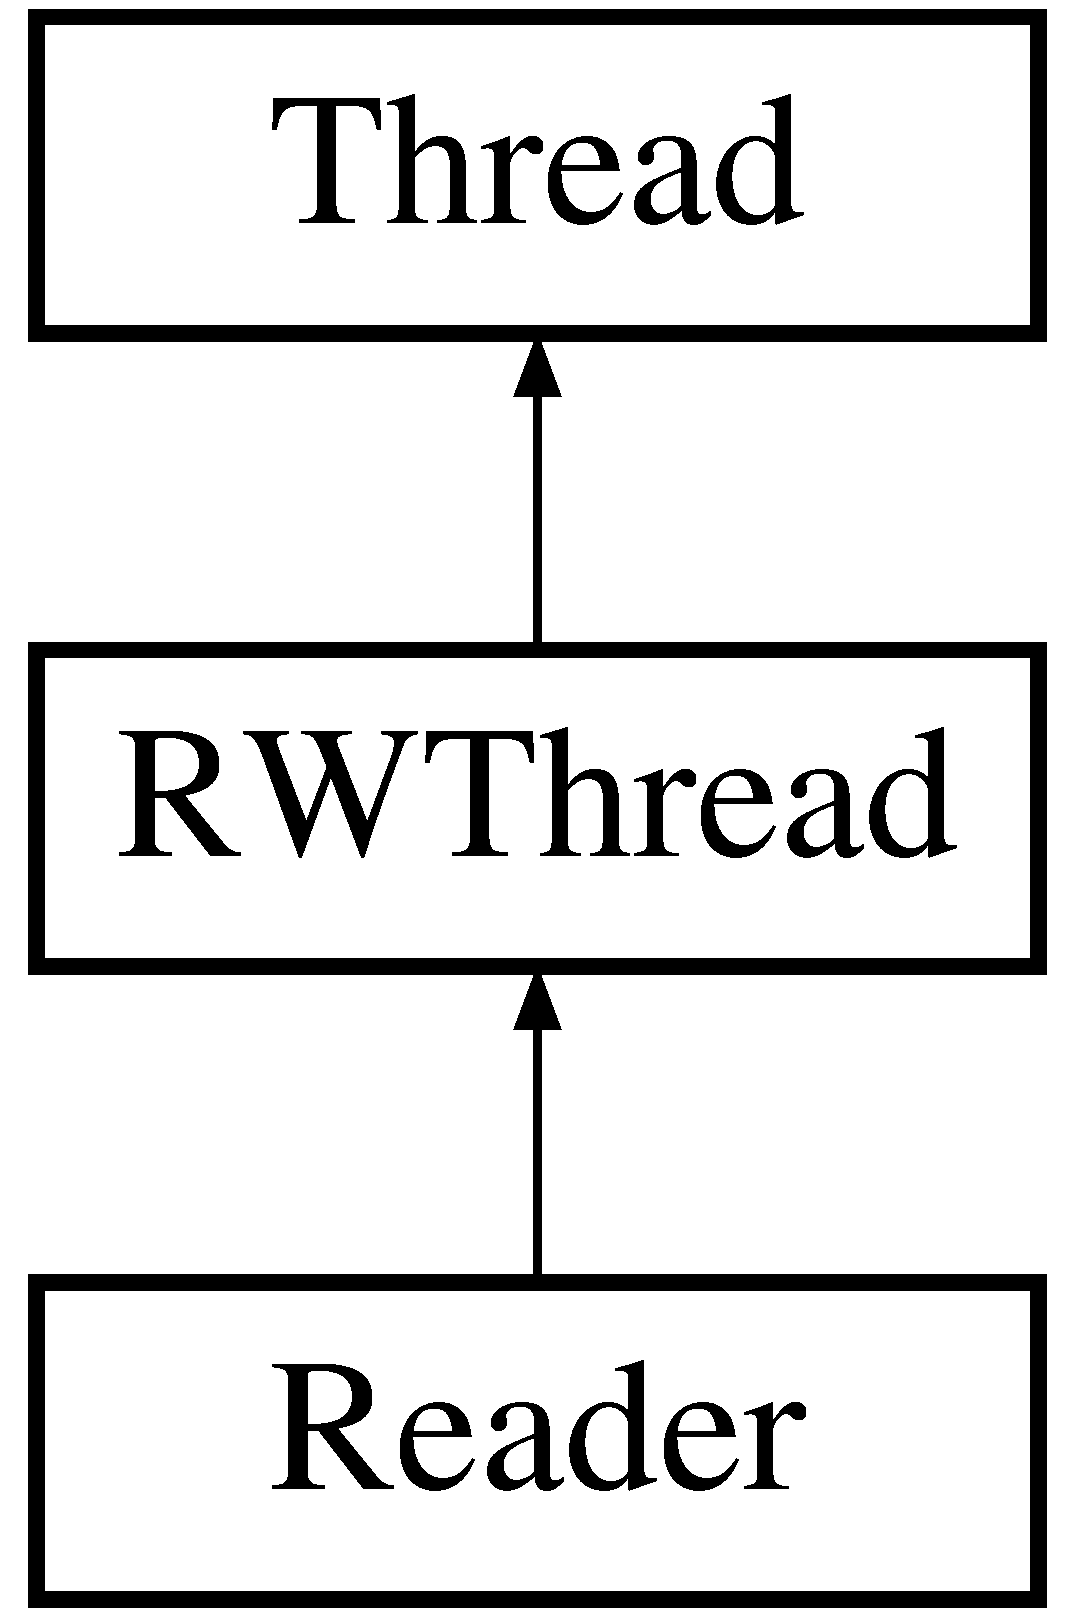
\includegraphics[height=3.000000cm]{class_reader}
\end{center}
\end{figure}
\subsection*{Public Member Functions}
\begin{DoxyCompactItemize}
\item 
\hyperlink{class_reader_adcda31b507720ab44044d7a21686fba2}{Reader} ()
\begin{DoxyCompactList}\small\item\em Default-\/constructor for the \hyperlink{class_reader}{Reader} class. \end{DoxyCompactList}\item 
\hyperlink{class_reader_a5c2576afadd1be193f99fb6d54787b56}{Reader} (\hyperlink{class_r_w_database}{R\+W\+Database}$<$ \hyperlink{classtsgl_1_1_rectangle}{Rectangle} $\ast$$>$ \&shared\+Database, \hyperlink{class_lock}{Lock} \&lock, unsigned long id, \hyperlink{classtsgl_1_1_canvas}{Canvas} \&can)
\begin{DoxyCompactList}\small\item\em Explicit-\/constructor for the \hyperlink{class_reader}{Reader} class. \end{DoxyCompactList}\item 
\mbox{\Hypertarget{class_reader_a83d805383b755b46f43491f8a0c8f3f8}\label{class_reader_a83d805383b755b46f43491f8a0c8f3f8}} 
void {\bfseries lock} ()
\item 
\mbox{\Hypertarget{class_reader_a89f5f3c7107185ac9a8d54c6464b7ee3}\label{class_reader_a89f5f3c7107185ac9a8d54c6464b7ee3}} 
void {\bfseries act} ()
\item 
\mbox{\Hypertarget{class_reader_ae6fdb55ccd1f482824e64f72c65b83e0}\label{class_reader_ae6fdb55ccd1f482824e64f72c65b83e0}} 
void {\bfseries unlock} ()
\end{DoxyCompactItemize}
\subsection*{Additional Inherited Members}


\subsection{Detailed Description}
\hyperlink{class_reader}{Reader} class inherits from the \hyperlink{class_r_w_thread}{R\+W\+Thread} class in order to create a \hyperlink{class_reader}{Reader} object. 

Inheritance\+: \hyperlink{class_r_w_thread}{R\+W\+Thread} class.

Implements the run() method, which calls the read() method. 

\subsection{Constructor \& Destructor Documentation}
\mbox{\Hypertarget{class_reader_adcda31b507720ab44044d7a21686fba2}\label{class_reader_adcda31b507720ab44044d7a21686fba2}} 
\index{Reader@{Reader}!Reader@{Reader}}
\index{Reader@{Reader}!Reader@{Reader}}
\subsubsection{\texorpdfstring{Reader()}{Reader()}\hspace{0.1cm}{\footnotesize\ttfamily [1/2]}}
{\footnotesize\ttfamily Reader\+::\+Reader (\begin{DoxyParamCaption}{ }\end{DoxyParamCaption})}



Default-\/constructor for the \hyperlink{class_reader}{Reader} class. 

\begin{DoxyReturn}{Returns}
\+: The constructed \hyperlink{class_reader}{Reader} object. 
\end{DoxyReturn}
\mbox{\Hypertarget{class_reader_a5c2576afadd1be193f99fb6d54787b56}\label{class_reader_a5c2576afadd1be193f99fb6d54787b56}} 
\index{Reader@{Reader}!Reader@{Reader}}
\index{Reader@{Reader}!Reader@{Reader}}
\subsubsection{\texorpdfstring{Reader()}{Reader()}\hspace{0.1cm}{\footnotesize\ttfamily [2/2]}}
{\footnotesize\ttfamily Reader\+::\+Reader (\begin{DoxyParamCaption}\item[{\hyperlink{class_r_w_database}{R\+W\+Database}$<$ \hyperlink{classtsgl_1_1_rectangle}{Rectangle} $\ast$$>$ \&}]{shared\+Database,  }\item[{\hyperlink{class_lock}{Lock} \&}]{lock,  }\item[{unsigned long}]{id,  }\item[{\hyperlink{classtsgl_1_1_canvas}{Canvas} \&}]{can }\end{DoxyParamCaption})}



Explicit-\/constructor for the \hyperlink{class_reader}{Reader} class. 


\begin{DoxyParams}{Parameters}
{\em } & \\
\hline
\end{DoxyParams}


The documentation for this class was generated from the following files\+:\begin{DoxyCompactItemize}
\item 
/home/sth5/test/\+T\+S\+G\+L/src/examples/\+Reader\+Writer/Reader.\+h\item 
/home/sth5/test/\+T\+S\+G\+L/src/examples/\+Reader\+Writer/Reader.\+cpp\end{DoxyCompactItemize}

\hypertarget{classtsgl_1_1_rectangle}{}\section{tsgl\+:\+:Rectangle Class Reference}
\label{classtsgl_1_1_rectangle}\index{tsgl\+::\+Rectangle@{tsgl\+::\+Rectangle}}


Draw a simple \hyperlink{classtsgl_1_1_rectangle}{Rectangle}.  




{\ttfamily \#include $<$Rectangle.\+h$>$}

Inheritance diagram for tsgl\+:\+:Rectangle\+:\begin{figure}[H]
\begin{center}
\leavevmode
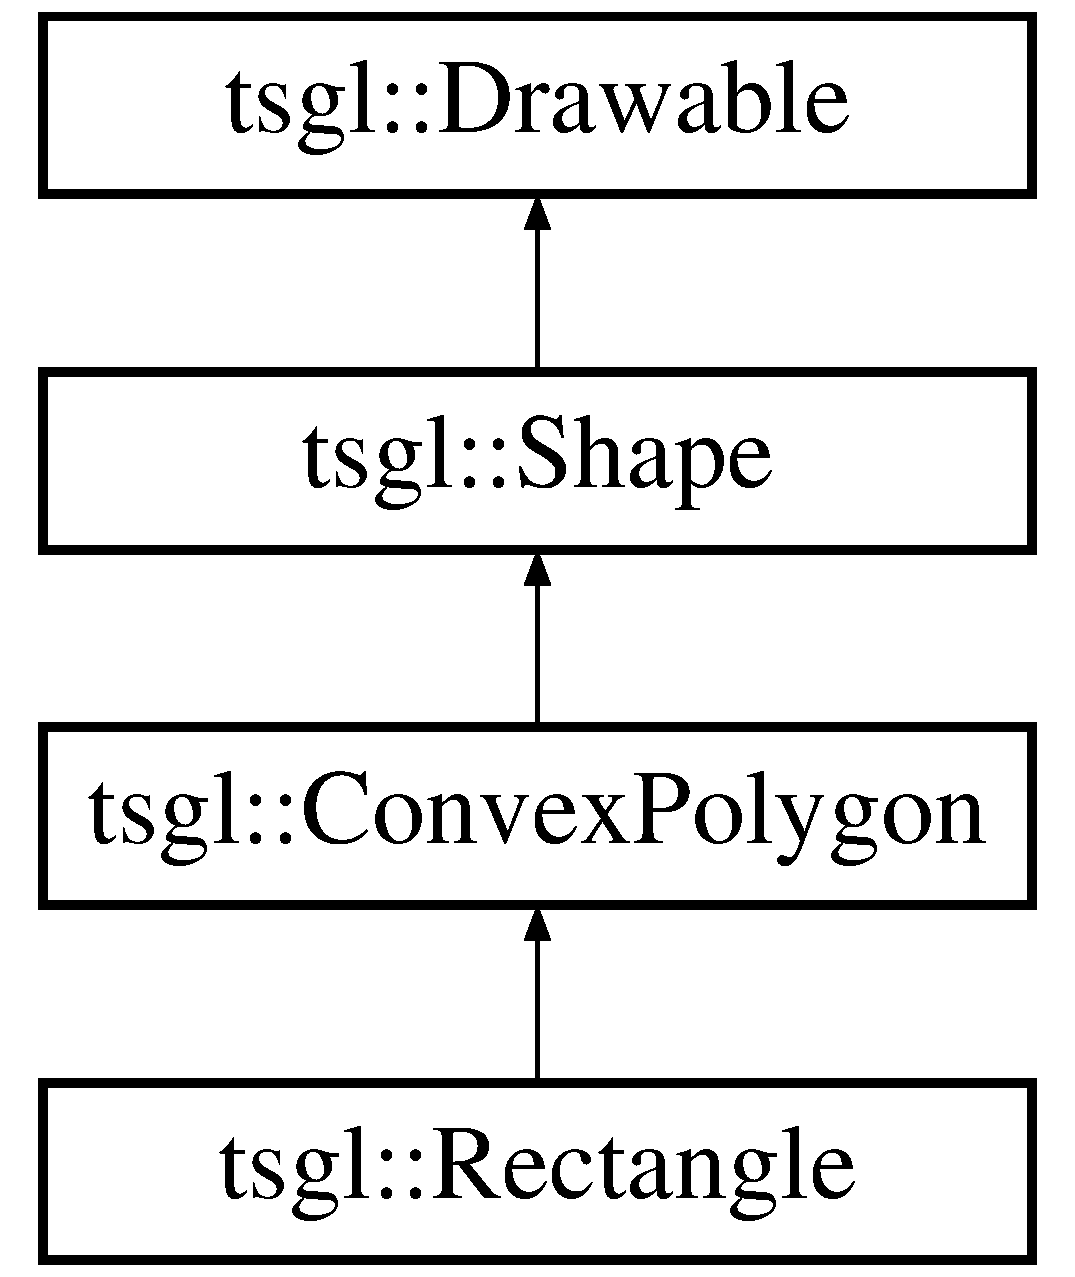
\includegraphics[height=2.000000cm]{classtsgl_1_1_rectangle}
\end{center}
\end{figure}
\subsection*{Public Member Functions}
\begin{DoxyCompactItemize}
\item 
\hyperlink{classtsgl_1_1_rectangle_a571dd054c2a10a55bd61fd7f43bc872d}{Rectangle} (int x, int y, int w, int h, const \hyperlink{structtsgl_1_1_color_float}{Color\+Float} \&color)
\begin{DoxyCompactList}\small\item\em Explicitly constructs a \hyperlink{classtsgl_1_1_rectangle}{Rectangle}. \end{DoxyCompactList}\item 
void \hyperlink{classtsgl_1_1_rectangle_addad1e65bc50d3669e6350aa32249c7f}{draw} ()
\begin{DoxyCompactList}\small\item\em Draw the \hyperlink{classtsgl_1_1_rectangle}{Rectangle}. \end{DoxyCompactList}\end{DoxyCompactItemize}
\subsection*{Additional Inherited Members}


\subsection{Detailed Description}
Draw a simple \hyperlink{classtsgl_1_1_rectangle}{Rectangle}. 

\hyperlink{classtsgl_1_1_rectangle}{Rectangle} is a class for holding vertex data for a simple rectangle. 

\subsection{Constructor \& Destructor Documentation}
\hypertarget{classtsgl_1_1_rectangle_a571dd054c2a10a55bd61fd7f43bc872d}{}\index{tsgl\+::\+Rectangle@{tsgl\+::\+Rectangle}!Rectangle@{Rectangle}}
\index{Rectangle@{Rectangle}!tsgl\+::\+Rectangle@{tsgl\+::\+Rectangle}}
\subsubsection[{Rectangle}]{\setlength{\rightskip}{0pt plus 5cm}tsgl\+::\+Rectangle\+::\+Rectangle (
\begin{DoxyParamCaption}
\item[{int}]{x, }
\item[{int}]{y, }
\item[{int}]{w, }
\item[{int}]{h, }
\item[{const {\bf Color\+Float} \&}]{color}
\end{DoxyParamCaption}
)}\label{classtsgl_1_1_rectangle_a571dd054c2a10a55bd61fd7f43bc872d}


Explicitly constructs a \hyperlink{classtsgl_1_1_rectangle}{Rectangle}. 

This is the constructor for the \hyperlink{classtsgl_1_1_rectangle}{Rectangle} class. 
\begin{DoxyParams}{Parameters}
{\em x} & The x coordinate of the \hyperlink{classtsgl_1_1_rectangle}{Rectangle}\textquotesingle{}s left edge. \\
\hline
{\em y} & The y coordinate of the \hyperlink{classtsgl_1_1_rectangle}{Rectangle}\textquotesingle{}s top edge. \\
\hline
{\em w} & The width of the \hyperlink{classtsgl_1_1_rectangle}{Rectangle}. \\
\hline
{\em h} & The height of the \hyperlink{classtsgl_1_1_rectangle}{Rectangle}. \\
\hline
{\em color} & The color of the \hyperlink{classtsgl_1_1_rectangle}{Rectangle}. \\
\hline
\end{DoxyParams}
\begin{DoxyReturn}{Returns}
A new \hyperlink{classtsgl_1_1_rectangle}{Rectangle} with the specified top left corner, dimensions, and color. 
\end{DoxyReturn}


\subsection{Member Function Documentation}
\hypertarget{classtsgl_1_1_rectangle_addad1e65bc50d3669e6350aa32249c7f}{}\index{tsgl\+::\+Rectangle@{tsgl\+::\+Rectangle}!draw@{draw}}
\index{draw@{draw}!tsgl\+::\+Rectangle@{tsgl\+::\+Rectangle}}
\subsubsection[{draw}]{\setlength{\rightskip}{0pt plus 5cm}void tsgl\+::\+Rectangle\+::draw (
\begin{DoxyParamCaption}
{}
\end{DoxyParamCaption}
)\hspace{0.3cm}{\ttfamily [virtual]}}\label{classtsgl_1_1_rectangle_addad1e65bc50d3669e6350aa32249c7f}


Draw the \hyperlink{classtsgl_1_1_rectangle}{Rectangle}. 

This function actually draws the \hyperlink{classtsgl_1_1_rectangle}{Rectangle} to the \hyperlink{classtsgl_1_1_canvas}{Canvas}. 

Implements \hyperlink{classtsgl_1_1_shape_af78b1627b97d621824ce86db214e2402}{tsgl\+::\+Shape}.



The documentation for this class was generated from the following files\+:\begin{DoxyCompactItemize}
\item 
Rectangle.\+h\item 
Rectangle.\+cpp\end{DoxyCompactItemize}

\hypertarget{classtsgl_1_1_regular_polygon}{}\section{tsgl\+:\+:Regular\+Polygon Class Reference}
\label{classtsgl_1_1_regular_polygon}\index{tsgl\+::\+Regular\+Polygon@{tsgl\+::\+Regular\+Polygon}}


Draw a regular polygon.  




{\ttfamily \#include $<$Regular\+Polygon.\+h$>$}

Inheritance diagram for tsgl\+:\+:Regular\+Polygon\+:\begin{figure}[H]
\begin{center}
\leavevmode
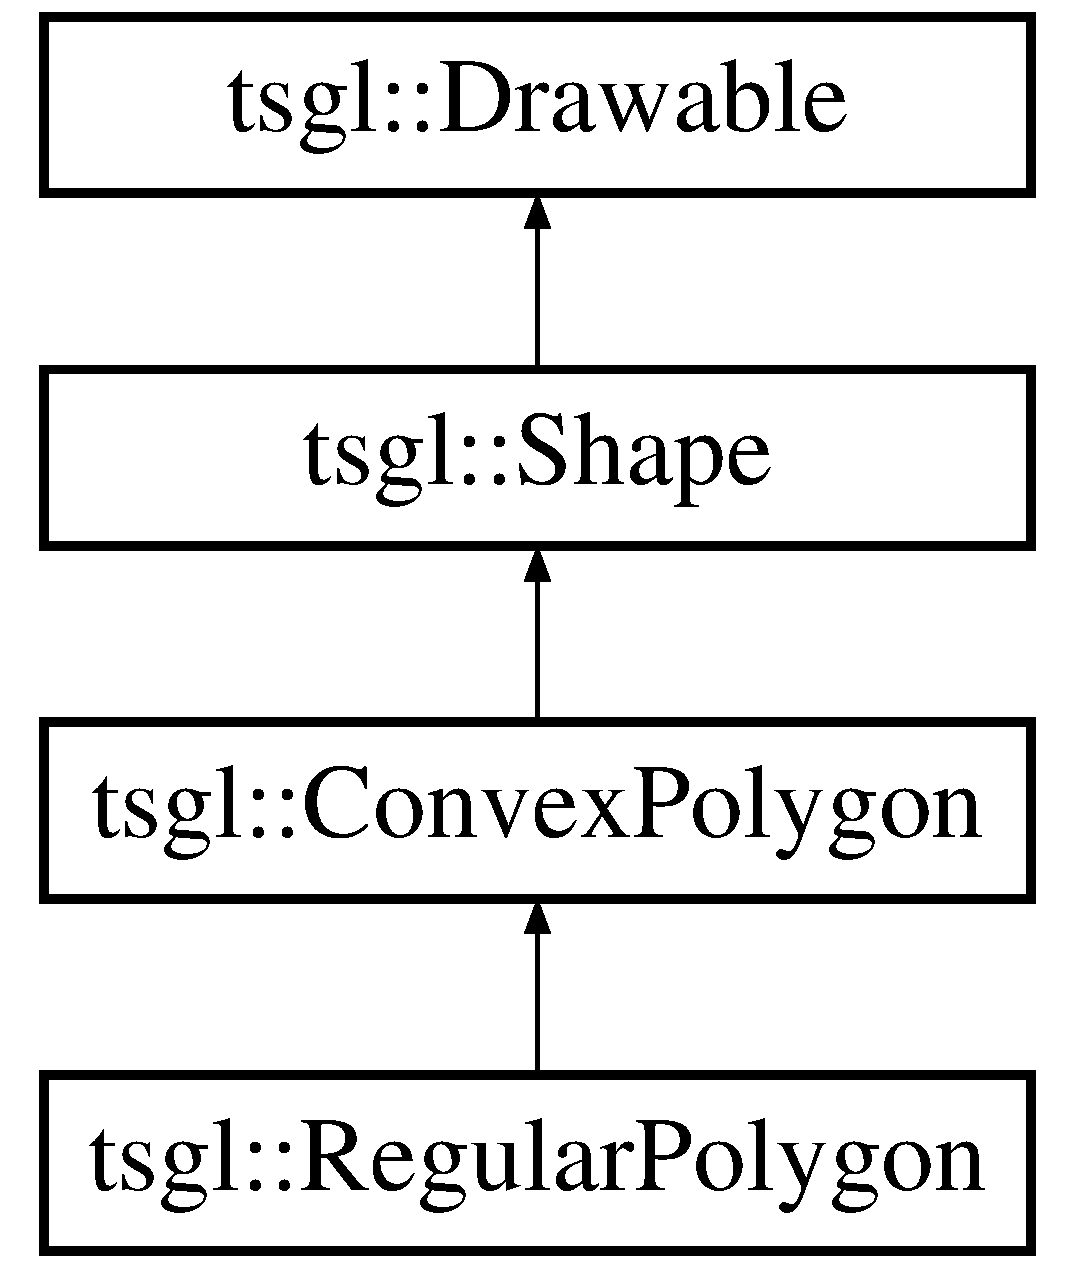
\includegraphics[height=4.000000cm]{classtsgl_1_1_regular_polygon}
\end{center}
\end{figure}
\subsection*{Public Member Functions}
\begin{DoxyCompactItemize}
\item 
\hyperlink{classtsgl_1_1_regular_polygon_a084a058facd0ce8576c908227c912f72}{Regular\+Polygon} (float x, float y, float z, G\+Lfloat radius, int sides, float yaw, float pitch, float roll, \hyperlink{structtsgl_1_1_color_float}{Color\+Float} color)
\begin{DoxyCompactList}\small\item\em Explicitly constructs a new \hyperlink{classtsgl_1_1_regular_polygon}{Regular\+Polygon} with monocolored fill. \end{DoxyCompactList}\item 
\hyperlink{classtsgl_1_1_regular_polygon_aba7efbdad969dcd3a176b55bd8b545b0}{Regular\+Polygon} (float x, float y, float z, G\+Lfloat radius, int sides, float yaw, float pitch, float roll, \hyperlink{structtsgl_1_1_color_float}{Color\+Float} color\mbox{[}$\,$\mbox{]})
\begin{DoxyCompactList}\small\item\em Explicitly constructs a new \hyperlink{classtsgl_1_1_regular_polygon}{Regular\+Polygon} with multicolored fill. \end{DoxyCompactList}\item 
int \hyperlink{classtsgl_1_1_regular_polygon_ac3f500be681b6d43f75ec00bf5434be0}{get\+Sides} ()
\begin{DoxyCompactList}\small\item\em Accessor for the number of sides of the \hyperlink{classtsgl_1_1_regular_polygon}{Regular\+Polygon}. \end{DoxyCompactList}\item 
G\+Lfloat \hyperlink{classtsgl_1_1_regular_polygon_a97e19ebc76f1f22f5fee795d4d633aa0}{get\+Radius} ()
\begin{DoxyCompactList}\small\item\em Accessor for the radius of the \hyperlink{classtsgl_1_1_regular_polygon}{Regular\+Polygon}. \end{DoxyCompactList}\item 
void \hyperlink{classtsgl_1_1_regular_polygon_a3c4240fc8d95e6875fc716b26504000e}{set\+Radius} (G\+Lfloat radius)
\begin{DoxyCompactList}\small\item\em Mutates the distance from the center of the \hyperlink{classtsgl_1_1_regular_polygon}{Regular\+Polygon} base to its vertices. \end{DoxyCompactList}\item 
void \hyperlink{classtsgl_1_1_regular_polygon_af115ff2fbff6075dc965af51f7507bc9}{change\+Radius\+By} (G\+Lfloat delta)
\begin{DoxyCompactList}\small\item\em Mutates the distance from the center of the \hyperlink{classtsgl_1_1_regular_polygon}{Regular\+Polygon} to its vertices by the parameter amount. \end{DoxyCompactList}\end{DoxyCompactItemize}
\subsection*{Protected Attributes}
\begin{DoxyCompactItemize}
\item 
\mbox{\Hypertarget{classtsgl_1_1_regular_polygon_a11297204087159c74683b7ba92b703b8}\label{classtsgl_1_1_regular_polygon_a11297204087159c74683b7ba92b703b8}} 
G\+Lfloat {\bfseries my\+Radius}
\item 
\mbox{\Hypertarget{classtsgl_1_1_regular_polygon_af84c48c2e6ff8a6d389e73c4185655b7}\label{classtsgl_1_1_regular_polygon_af84c48c2e6ff8a6d389e73c4185655b7}} 
int {\bfseries my\+Sides}
\end{DoxyCompactItemize}
\subsection*{Additional Inherited Members}


\subsection{Detailed Description}
Draw a regular polygon. 

\hyperlink{classtsgl_1_1_regular_polygon}{Regular\+Polygon} is a class for holding \hyperlink{classtsgl_1_1_convex_polygon}{Convex\+Polygon} data for a regular polygon. 

\subsection{Constructor \& Destructor Documentation}
\mbox{\Hypertarget{classtsgl_1_1_regular_polygon_a084a058facd0ce8576c908227c912f72}\label{classtsgl_1_1_regular_polygon_a084a058facd0ce8576c908227c912f72}} 
\index{tsgl\+::\+Regular\+Polygon@{tsgl\+::\+Regular\+Polygon}!Regular\+Polygon@{Regular\+Polygon}}
\index{Regular\+Polygon@{Regular\+Polygon}!tsgl\+::\+Regular\+Polygon@{tsgl\+::\+Regular\+Polygon}}
\subsubsection{\texorpdfstring{Regular\+Polygon()}{RegularPolygon()}\hspace{0.1cm}{\footnotesize\ttfamily [1/2]}}
{\footnotesize\ttfamily tsgl\+::\+Regular\+Polygon\+::\+Regular\+Polygon (\begin{DoxyParamCaption}\item[{float}]{x,  }\item[{float}]{y,  }\item[{float}]{z,  }\item[{G\+Lfloat}]{radius,  }\item[{int}]{sides,  }\item[{float}]{yaw,  }\item[{float}]{pitch,  }\item[{float}]{roll,  }\item[{\hyperlink{structtsgl_1_1_color_float}{Color\+Float}}]{color }\end{DoxyParamCaption})}



Explicitly constructs a new \hyperlink{classtsgl_1_1_regular_polygon}{Regular\+Polygon} with monocolored fill. 

This function draws a regular polygon with the given center, sides, radius, rotation, and color. (number of sides), and color. 
\begin{DoxyParams}{Parameters}
{\em x} & The x coordinate of the \hyperlink{classtsgl_1_1_regular_polygon}{Regular\+Polygon}\textquotesingle{}s center. \\
\hline
{\em y} & The y coordinate of the \hyperlink{classtsgl_1_1_regular_polygon}{Regular\+Polygon}\textquotesingle{}s center. \\
\hline
{\em z} & The z coordinate of the \hyperlink{classtsgl_1_1_regular_polygon}{Regular\+Polygon}\textquotesingle{}s center. \\
\hline
{\em radius} & The radius of the \hyperlink{classtsgl_1_1_regular_polygon}{Regular\+Polygon} in pixels. \\
\hline
{\em sides} & The number of sides to use in the \hyperlink{classtsgl_1_1_regular_polygon}{Regular\+Polygon}. \\
\hline
{\em yaw} & The \hyperlink{classtsgl_1_1_regular_polygon}{Regular\+Polygon}\textquotesingle{}s yaw in 3D space. \\
\hline
{\em pitch} & The \hyperlink{classtsgl_1_1_regular_polygon}{Regular\+Polygon}\textquotesingle{}s pitch in 3D space. \\
\hline
{\em roll} & The \hyperlink{classtsgl_1_1_regular_polygon}{Regular\+Polygon}\textquotesingle{}s roll in 3D space. \\
\hline
{\em color} & The color of the \hyperlink{classtsgl_1_1_regular_polygon}{Regular\+Polygon}. \\
\hline
\end{DoxyParams}
\mbox{\Hypertarget{classtsgl_1_1_regular_polygon_aba7efbdad969dcd3a176b55bd8b545b0}\label{classtsgl_1_1_regular_polygon_aba7efbdad969dcd3a176b55bd8b545b0}} 
\index{tsgl\+::\+Regular\+Polygon@{tsgl\+::\+Regular\+Polygon}!Regular\+Polygon@{Regular\+Polygon}}
\index{Regular\+Polygon@{Regular\+Polygon}!tsgl\+::\+Regular\+Polygon@{tsgl\+::\+Regular\+Polygon}}
\subsubsection{\texorpdfstring{Regular\+Polygon()}{RegularPolygon()}\hspace{0.1cm}{\footnotesize\ttfamily [2/2]}}
{\footnotesize\ttfamily tsgl\+::\+Regular\+Polygon\+::\+Regular\+Polygon (\begin{DoxyParamCaption}\item[{float}]{x,  }\item[{float}]{y,  }\item[{float}]{z,  }\item[{G\+Lfloat}]{radius,  }\item[{int}]{sides,  }\item[{float}]{yaw,  }\item[{float}]{pitch,  }\item[{float}]{roll,  }\item[{\hyperlink{structtsgl_1_1_color_float}{Color\+Float}}]{color\mbox{[}$\,$\mbox{]} }\end{DoxyParamCaption})}



Explicitly constructs a new \hyperlink{classtsgl_1_1_regular_polygon}{Regular\+Polygon} with multicolored fill. 

This function draws a regular polygon with the given center, sides, radius, rotation, and color. (number of sides), and coloring. 
\begin{DoxyParams}{Parameters}
{\em x} & The x coordinate of the \hyperlink{classtsgl_1_1_regular_polygon}{Regular\+Polygon}\textquotesingle{}s center. \\
\hline
{\em y} & The y coordinate of the \hyperlink{classtsgl_1_1_regular_polygon}{Regular\+Polygon}\textquotesingle{}s center. \\
\hline
{\em z} & The z coordinate of the \hyperlink{classtsgl_1_1_regular_polygon}{Regular\+Polygon}\textquotesingle{}s center. \\
\hline
{\em radius} & The radius of the \hyperlink{classtsgl_1_1_regular_polygon}{Regular\+Polygon} in pixels. \\
\hline
{\em sides} & The number of sides to use in the \hyperlink{classtsgl_1_1_regular_polygon}{Regular\+Polygon}. \\
\hline
{\em yaw} & The \hyperlink{classtsgl_1_1_regular_polygon}{Regular\+Polygon}\textquotesingle{}s yaw in 3D space. \\
\hline
{\em pitch} & The \hyperlink{classtsgl_1_1_regular_polygon}{Regular\+Polygon}\textquotesingle{}s pitch in 3D space. \\
\hline
{\em roll} & The \hyperlink{classtsgl_1_1_regular_polygon}{Regular\+Polygon}\textquotesingle{}s roll in 3D space. \\
\hline
{\em color} & An array of colors for the regular polygon\textquotesingle{}s vertices. \\
\hline
\end{DoxyParams}


\subsection{Member Function Documentation}
\mbox{\Hypertarget{classtsgl_1_1_regular_polygon_af115ff2fbff6075dc965af51f7507bc9}\label{classtsgl_1_1_regular_polygon_af115ff2fbff6075dc965af51f7507bc9}} 
\index{tsgl\+::\+Regular\+Polygon@{tsgl\+::\+Regular\+Polygon}!change\+Radius\+By@{change\+Radius\+By}}
\index{change\+Radius\+By@{change\+Radius\+By}!tsgl\+::\+Regular\+Polygon@{tsgl\+::\+Regular\+Polygon}}
\subsubsection{\texorpdfstring{change\+Radius\+By()}{changeRadiusBy()}}
{\footnotesize\ttfamily void tsgl\+::\+Regular\+Polygon\+::change\+Radius\+By (\begin{DoxyParamCaption}\item[{G\+Lfloat}]{delta }\end{DoxyParamCaption})}



Mutates the distance from the center of the \hyperlink{classtsgl_1_1_regular_polygon}{Regular\+Polygon} to its vertices by the parameter amount. 


\begin{DoxyParams}{Parameters}
{\em delta} & The amount by which to change the radius of the \hyperlink{classtsgl_1_1_regular_polygon}{Regular\+Polygon}. \\
\hline
\end{DoxyParams}


Referenced by get\+Radius().

\mbox{\Hypertarget{classtsgl_1_1_regular_polygon_a97e19ebc76f1f22f5fee795d4d633aa0}\label{classtsgl_1_1_regular_polygon_a97e19ebc76f1f22f5fee795d4d633aa0}} 
\index{tsgl\+::\+Regular\+Polygon@{tsgl\+::\+Regular\+Polygon}!get\+Radius@{get\+Radius}}
\index{get\+Radius@{get\+Radius}!tsgl\+::\+Regular\+Polygon@{tsgl\+::\+Regular\+Polygon}}
\subsubsection{\texorpdfstring{get\+Radius()}{getRadius()}}
{\footnotesize\ttfamily G\+Lfloat tsgl\+::\+Regular\+Polygon\+::get\+Radius (\begin{DoxyParamCaption}{ }\end{DoxyParamCaption})\hspace{0.3cm}{\ttfamily [inline]}}



Accessor for the radius of the \hyperlink{classtsgl_1_1_regular_polygon}{Regular\+Polygon}. 

Returns the value of the my\+Radius private variable, a G\+Lfloat. \mbox{\Hypertarget{classtsgl_1_1_regular_polygon_ac3f500be681b6d43f75ec00bf5434be0}\label{classtsgl_1_1_regular_polygon_ac3f500be681b6d43f75ec00bf5434be0}} 
\index{tsgl\+::\+Regular\+Polygon@{tsgl\+::\+Regular\+Polygon}!get\+Sides@{get\+Sides}}
\index{get\+Sides@{get\+Sides}!tsgl\+::\+Regular\+Polygon@{tsgl\+::\+Regular\+Polygon}}
\subsubsection{\texorpdfstring{get\+Sides()}{getSides()}}
{\footnotesize\ttfamily int tsgl\+::\+Regular\+Polygon\+::get\+Sides (\begin{DoxyParamCaption}{ }\end{DoxyParamCaption})\hspace{0.3cm}{\ttfamily [inline]}}



Accessor for the number of sides of the \hyperlink{classtsgl_1_1_regular_polygon}{Regular\+Polygon}. 

Returns the value of the my\+Sides private variable, an int. \mbox{\Hypertarget{classtsgl_1_1_regular_polygon_a3c4240fc8d95e6875fc716b26504000e}\label{classtsgl_1_1_regular_polygon_a3c4240fc8d95e6875fc716b26504000e}} 
\index{tsgl\+::\+Regular\+Polygon@{tsgl\+::\+Regular\+Polygon}!set\+Radius@{set\+Radius}}
\index{set\+Radius@{set\+Radius}!tsgl\+::\+Regular\+Polygon@{tsgl\+::\+Regular\+Polygon}}
\subsubsection{\texorpdfstring{set\+Radius()}{setRadius()}}
{\footnotesize\ttfamily void tsgl\+::\+Regular\+Polygon\+::set\+Radius (\begin{DoxyParamCaption}\item[{G\+Lfloat}]{radius }\end{DoxyParamCaption})}



Mutates the distance from the center of the \hyperlink{classtsgl_1_1_regular_polygon}{Regular\+Polygon} base to its vertices. 


\begin{DoxyParams}{Parameters}
{\em radius} & The \hyperlink{classtsgl_1_1_regular_polygon}{Regular\+Polygon}\textquotesingle{}s new radius. \\
\hline
\end{DoxyParams}


Referenced by get\+Radius().



The documentation for this class was generated from the following files\+:\begin{DoxyCompactItemize}
\item 
Regular\+Polygon.\+h\item 
Regular\+Polygon.\+cpp\end{DoxyCompactItemize}

\hypertarget{class_r_lock}{}\section{R\+Lock Class Reference}
\label{class_r_lock}\index{R\+Lock@{R\+Lock}}


A lock giving priority to Readers.  




{\ttfamily \#include $<$R\+Lock.\+h$>$}

Inheritance diagram for R\+Lock\+:\begin{figure}[H]
\begin{center}
\leavevmode
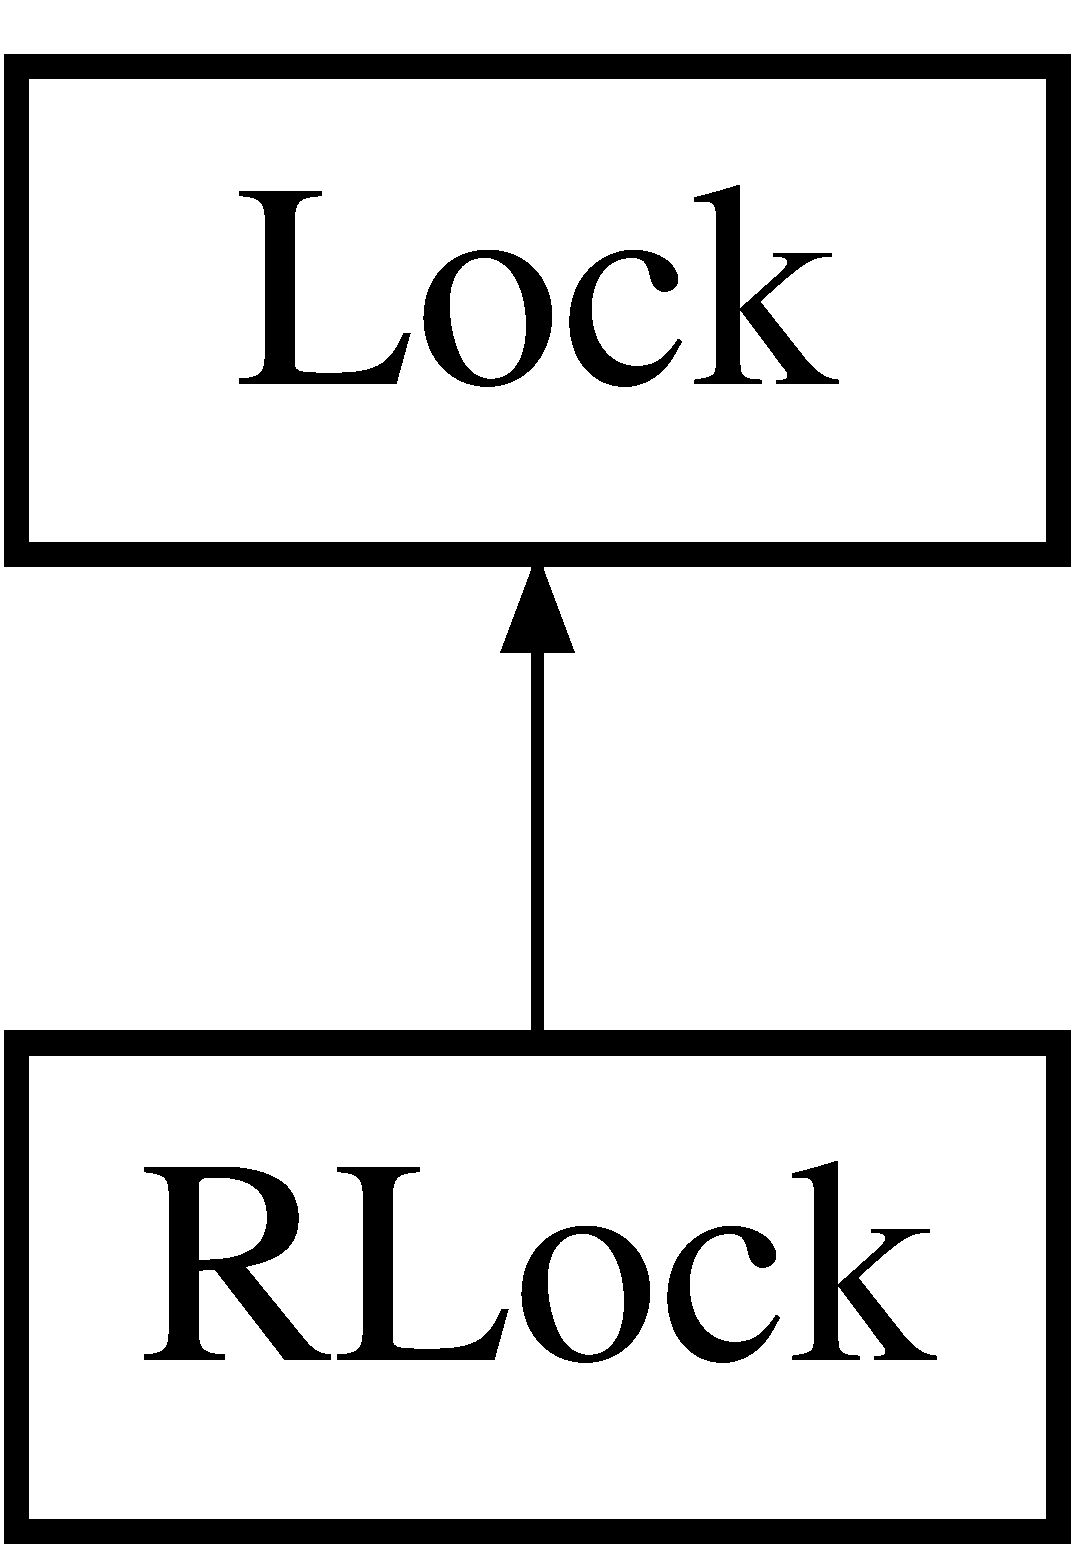
\includegraphics[height=2.000000cm]{class_r_lock}
\end{center}
\end{figure}
\subsection*{Public Member Functions}
\begin{DoxyCompactItemize}
\item 
\mbox{\Hypertarget{class_r_lock_a94f2c0fcd95500addf4d8dd124e1a2cd}\label{class_r_lock_a94f2c0fcd95500addf4d8dd124e1a2cd}} 
{\bfseries R\+Lock} (\hyperlink{class_r_w_database}{R\+W\+Database}$<$ \hyperlink{classtsgl_1_1_rectangle}{tsgl\+::\+Rectangle} $\ast$$>$ $\ast$data)
\item 
void \hyperlink{class_r_lock_a6445aacde1dc9a6f7769d1b1480d6162}{read\+Lock} ()
\begin{DoxyCompactList}\small\item\em \hyperlink{class_r_lock_a6445aacde1dc9a6f7769d1b1480d6162}{read\+Lock()} implements the abstract method in \hyperlink{class_lock}{Lock} \end{DoxyCompactList}\item 
void \hyperlink{class_r_lock_a0af51edce04598b0afe551d356cfe05b}{read\+Unlock} ()
\begin{DoxyCompactList}\small\item\em \hyperlink{class_r_lock_a0af51edce04598b0afe551d356cfe05b}{read\+Unlock()} implements the abstract method in \hyperlink{class_lock}{Lock} \end{DoxyCompactList}\item 
void \hyperlink{class_r_lock_ab04d415f49f28f6a8198f611d03e9bcd}{write\+Lock} ()
\begin{DoxyCompactList}\small\item\em \hyperlink{class_r_lock_ab04d415f49f28f6a8198f611d03e9bcd}{write\+Lock()} implements the abstract method in \hyperlink{class_lock}{Lock} \end{DoxyCompactList}\item 
void \hyperlink{class_r_lock_a4c69e6a1922b1aab3a84afeececad3fa}{write\+Unlock} ()
\begin{DoxyCompactList}\small\item\em \hyperlink{class_r_lock_a4c69e6a1922b1aab3a84afeececad3fa}{write\+Unlock()} implements the abstract method in \hyperlink{class_lock}{Lock} \end{DoxyCompactList}\end{DoxyCompactItemize}
\subsection*{Additional Inherited Members}


\subsection{Detailed Description}
A lock giving priority to Readers. 

\hyperlink{_r_lock_8h_source}{R\+Lock.\+h} provides the monitor for the Reader-\/\+Writer visualization that gives preference to the Readers. This class is a subclass of \hyperlink{class_lock}{Lock} and implements its locking and unlocking virtual methods.

Inheritance\+: \hyperlink{class_lock}{Lock} class.

Implements the locking and unlocking methods of a monitor. 

\subsection{Member Function Documentation}
\mbox{\Hypertarget{class_r_lock_a6445aacde1dc9a6f7769d1b1480d6162}\label{class_r_lock_a6445aacde1dc9a6f7769d1b1480d6162}} 
\index{R\+Lock@{R\+Lock}!read\+Lock@{read\+Lock}}
\index{read\+Lock@{read\+Lock}!R\+Lock@{R\+Lock}}
\subsubsection{\texorpdfstring{read\+Lock()}{readLock()}}
{\footnotesize\ttfamily void R\+Lock\+::read\+Lock (\begin{DoxyParamCaption}{ }\end{DoxyParamCaption})\hspace{0.3cm}{\ttfamily [virtual]}}



\hyperlink{class_r_lock_a6445aacde1dc9a6f7769d1b1480d6162}{read\+Lock()} implements the abstract method in \hyperlink{class_lock}{Lock} 

R\+Lock.\+cpp provides the monitor for the Reader-\/\+Writer visualization that gives preference to the Readers. This class is a subclass of \hyperlink{class_lock}{Lock} and implements its locking and unlocking virtual methods.

Grants the calling thread access for reading, giving priority to readers 

Implements \hyperlink{class_lock}{Lock}.

\mbox{\Hypertarget{class_r_lock_a0af51edce04598b0afe551d356cfe05b}\label{class_r_lock_a0af51edce04598b0afe551d356cfe05b}} 
\index{R\+Lock@{R\+Lock}!read\+Unlock@{read\+Unlock}}
\index{read\+Unlock@{read\+Unlock}!R\+Lock@{R\+Lock}}
\subsubsection{\texorpdfstring{read\+Unlock()}{readUnlock()}}
{\footnotesize\ttfamily void R\+Lock\+::read\+Unlock (\begin{DoxyParamCaption}{ }\end{DoxyParamCaption})\hspace{0.3cm}{\ttfamily [virtual]}}



\hyperlink{class_r_lock_a0af51edce04598b0afe551d356cfe05b}{read\+Unlock()} implements the abstract method in \hyperlink{class_lock}{Lock} 

Releases the calling thread\textquotesingle{}s read lock 

Implements \hyperlink{class_lock}{Lock}.

\mbox{\Hypertarget{class_r_lock_ab04d415f49f28f6a8198f611d03e9bcd}\label{class_r_lock_ab04d415f49f28f6a8198f611d03e9bcd}} 
\index{R\+Lock@{R\+Lock}!write\+Lock@{write\+Lock}}
\index{write\+Lock@{write\+Lock}!R\+Lock@{R\+Lock}}
\subsubsection{\texorpdfstring{write\+Lock()}{writeLock()}}
{\footnotesize\ttfamily void R\+Lock\+::write\+Lock (\begin{DoxyParamCaption}{ }\end{DoxyParamCaption})\hspace{0.3cm}{\ttfamily [virtual]}}



\hyperlink{class_r_lock_ab04d415f49f28f6a8198f611d03e9bcd}{write\+Lock()} implements the abstract method in \hyperlink{class_lock}{Lock} 

Grants the calling thread acces for writing, giving priority to Readers 

Implements \hyperlink{class_lock}{Lock}.

\mbox{\Hypertarget{class_r_lock_a4c69e6a1922b1aab3a84afeececad3fa}\label{class_r_lock_a4c69e6a1922b1aab3a84afeececad3fa}} 
\index{R\+Lock@{R\+Lock}!write\+Unlock@{write\+Unlock}}
\index{write\+Unlock@{write\+Unlock}!R\+Lock@{R\+Lock}}
\subsubsection{\texorpdfstring{write\+Unlock()}{writeUnlock()}}
{\footnotesize\ttfamily void R\+Lock\+::write\+Unlock (\begin{DoxyParamCaption}{ }\end{DoxyParamCaption})\hspace{0.3cm}{\ttfamily [virtual]}}



\hyperlink{class_r_lock_a4c69e6a1922b1aab3a84afeececad3fa}{write\+Unlock()} implements the abstract method in \hyperlink{class_lock}{Lock} 

Releases the calling thread\textquotesingle{}s write lock 

Implements \hyperlink{class_lock}{Lock}.



The documentation for this class was generated from the following files\+:\begin{DoxyCompactItemize}
\item 
/home/sth5/test/\+T\+S\+G\+L/src/examples/\+Reader\+Writer/R\+Lock.\+h\item 
/home/sth5/test/\+T\+S\+G\+L/src/examples/\+Reader\+Writer/R\+Lock.\+cpp\end{DoxyCompactItemize}

\hypertarget{classtsgl_1_1_round_function}{}\section{tsgl\+:\+:Round\+Function Class Reference}
\label{classtsgl_1_1_round_function}\index{tsgl\+::\+Round\+Function@{tsgl\+::\+Round\+Function}}


\hyperlink{classtsgl_1_1_function}{Function} to round the input to the nearest integer number.  




{\ttfamily \#include $<$Function.\+h$>$}

Inheritance diagram for tsgl\+:\+:Round\+Function\+:\begin{figure}[H]
\begin{center}
\leavevmode
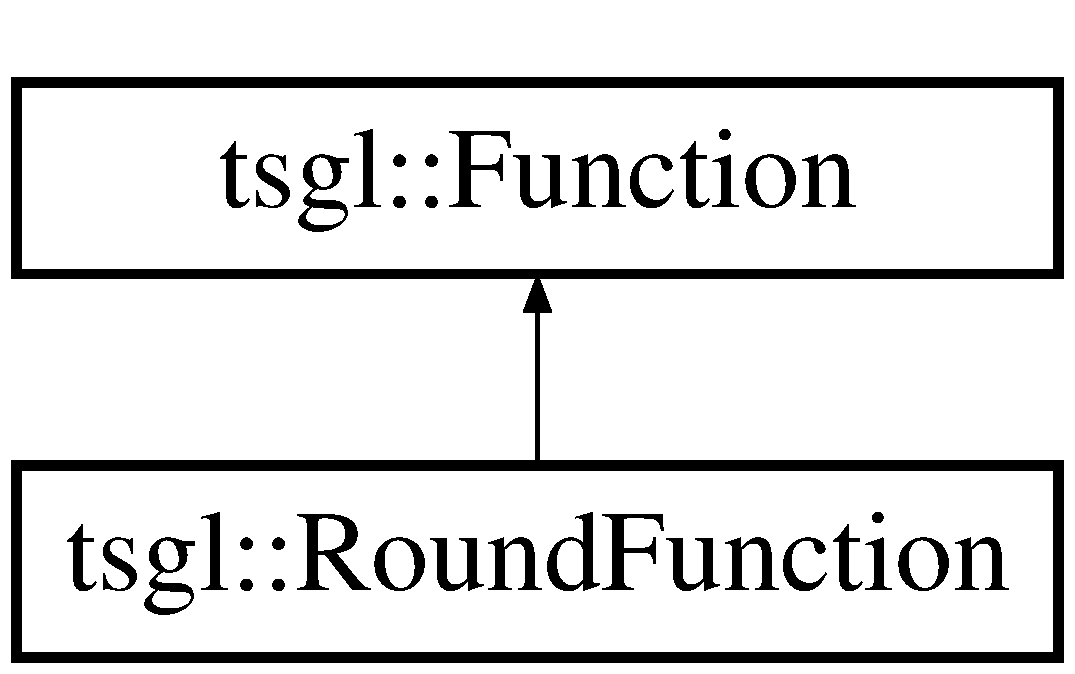
\includegraphics[height=2.000000cm]{classtsgl_1_1_round_function}
\end{center}
\end{figure}
\subsection*{Public Member Functions}
\begin{DoxyCompactItemize}
\item 
virtual Decimal \hyperlink{classtsgl_1_1_round_function_ad01ca0b18d7b5f3f8c5a49181b1dc922}{value\+At} (Decimal x) const
\begin{DoxyCompactList}\small\item\em Method to determine the value of \hyperlink{classtsgl_1_1_round_function}{Round\+Function}. \end{DoxyCompactList}\end{DoxyCompactItemize}


\subsection{Detailed Description}
\hyperlink{classtsgl_1_1_function}{Function} to round the input to the nearest integer number. 

\subsection{Member Function Documentation}
\mbox{\Hypertarget{classtsgl_1_1_round_function_ad01ca0b18d7b5f3f8c5a49181b1dc922}\label{classtsgl_1_1_round_function_ad01ca0b18d7b5f3f8c5a49181b1dc922}} 
\index{tsgl\+::\+Round\+Function@{tsgl\+::\+Round\+Function}!value\+At@{value\+At}}
\index{value\+At@{value\+At}!tsgl\+::\+Round\+Function@{tsgl\+::\+Round\+Function}}
\subsubsection{\texorpdfstring{value\+At()}{valueAt()}}
{\footnotesize\ttfamily virtual Decimal tsgl\+::\+Round\+Function\+::value\+At (\begin{DoxyParamCaption}\item[{Decimal}]{x }\end{DoxyParamCaption}) const\hspace{0.3cm}{\ttfamily [inline]}, {\ttfamily [virtual]}}



Method to determine the value of \hyperlink{classtsgl_1_1_round_function}{Round\+Function}. 

\begin{DoxyReturn}{Returns}
The closest integer to {\itshape x}. 
\end{DoxyReturn}


Implements \hyperlink{classtsgl_1_1_function_affb7b3b19a04efefa29a9870d666e912}{tsgl\+::\+Function}.



The documentation for this class was generated from the following file\+:\begin{DoxyCompactItemize}
\item 
Function.\+h\end{DoxyCompactItemize}

\hypertarget{class_r_w_database}{}\section{R\+W\+Database$<$ Item $>$ Class Template Reference}
\label{class_r_w_database}\index{R\+W\+Database$<$ Item $>$@{R\+W\+Database$<$ Item $>$}}


An abstract database protecting a vector of data.  




{\ttfamily \#include $<$R\+W\+Database.\+h$>$}

\subsection*{Public Member Functions}
\begin{DoxyCompactItemize}
\item 
\hyperlink{class_r_w_database_ab6e78a49fcfe2e296b7d7695c1404dd5}{R\+W\+Database} ()
\begin{DoxyCompactList}\small\item\em Default constructor for the \hyperlink{class_r_w_database}{R\+W\+Database} class. \end{DoxyCompactList}\item 
\hyperlink{class_r_w_database_aed3ea810bc64b4fcb41a8660b3a583de}{R\+W\+Database} (int max)
\begin{DoxyCompactList}\small\item\em Explicit constructor for the \hyperlink{class_r_w_database}{R\+W\+Database} class. \end{DoxyCompactList}\item 
\mbox{\Hypertarget{class_r_w_database_aa09d7c17e7741dcb480f052ff3689299}\label{class_r_w_database_aa09d7c17e7741dcb480f052ff3689299}} 
int {\bfseries get\+Item\+Count} ()
\item 
\mbox{\Hypertarget{class_r_w_database_a11a8f38b6a48e2ede789d0ed7081a737}\label{class_r_w_database_a11a8f38b6a48e2ede789d0ed7081a737}} 
int {\bfseries get\+Max\+Capacity} ()
\item 
Item \hyperlink{class_r_w_database_acb53aad02a38e6e021ba61f63b35ba9a}{read} (unsigned index)
\begin{DoxyCompactList}\small\item\em \hyperlink{class_r_w_database_acb53aad02a38e6e021ba61f63b35ba9a}{read()} returns the Item from the vector at an index \end{DoxyCompactList}\item 
void \hyperlink{class_r_w_database_acfdb85c4ae5201e9997265c6d44a3111}{write} (Item it, unsigned index)
\begin{DoxyCompactList}\small\item\em \hyperlink{class_r_w_database_acfdb85c4ae5201e9997265c6d44a3111}{write()} sets an item at an index \end{DoxyCompactList}\end{DoxyCompactItemize}
\subsection*{Protected Attributes}
\begin{DoxyCompactItemize}
\item 
\mbox{\Hypertarget{class_r_w_database_a27c74ad4eb0048078b6c395883fbf1e4}\label{class_r_w_database_a27c74ad4eb0048078b6c395883fbf1e4}} 
std\+::vector$<$ Item $>$ {\bfseries vec}
\item 
\mbox{\Hypertarget{class_r_w_database_a219c4621156200ef43c1508e16ee672f}\label{class_r_w_database_a219c4621156200ef43c1508e16ee672f}} 
unsigned {\bfseries max\+Capacity}
\end{DoxyCompactItemize}


\subsection{Detailed Description}
\subsubsection*{template$<$class Item$>$\newline
class R\+W\+Database$<$ Item $>$}

An abstract database protecting a vector of data. 

Database has its locks and a vector

Locking methods must be implemented in subclass, giving priority to different types of threads. 

\subsection{Constructor \& Destructor Documentation}
\mbox{\Hypertarget{class_r_w_database_ab6e78a49fcfe2e296b7d7695c1404dd5}\label{class_r_w_database_ab6e78a49fcfe2e296b7d7695c1404dd5}} 
\index{R\+W\+Database@{R\+W\+Database}!R\+W\+Database@{R\+W\+Database}}
\index{R\+W\+Database@{R\+W\+Database}!R\+W\+Database@{R\+W\+Database}}
\subsubsection{\texorpdfstring{R\+W\+Database()}{RWDatabase()}\hspace{0.1cm}{\footnotesize\ttfamily [1/2]}}
{\footnotesize\ttfamily template$<$class Item $>$ \\
\hyperlink{class_r_w_database}{R\+W\+Database}$<$ Item $>$\+::\hyperlink{class_r_w_database}{R\+W\+Database} (\begin{DoxyParamCaption}{ }\end{DoxyParamCaption})}



Default constructor for the \hyperlink{class_r_w_database}{R\+W\+Database} class. 

\begin{DoxyReturn}{Returns}
\+: The constructed \hyperlink{class_r_w_database}{R\+W\+Database} object. 
\end{DoxyReturn}
\mbox{\Hypertarget{class_r_w_database_aed3ea810bc64b4fcb41a8660b3a583de}\label{class_r_w_database_aed3ea810bc64b4fcb41a8660b3a583de}} 
\index{R\+W\+Database@{R\+W\+Database}!R\+W\+Database@{R\+W\+Database}}
\index{R\+W\+Database@{R\+W\+Database}!R\+W\+Database@{R\+W\+Database}}
\subsubsection{\texorpdfstring{R\+W\+Database()}{RWDatabase()}\hspace{0.1cm}{\footnotesize\ttfamily [2/2]}}
{\footnotesize\ttfamily template$<$class Item $>$ \\
\hyperlink{class_r_w_database}{R\+W\+Database}$<$ Item $>$\+::\hyperlink{class_r_w_database}{R\+W\+Database} (\begin{DoxyParamCaption}\item[{int}]{max }\end{DoxyParamCaption})}



Explicit constructor for the \hyperlink{class_r_w_database}{R\+W\+Database} class. 


\begin{DoxyParams}{Parameters}
{\em max,an} & int describing the maximum size of the contained vector \\
\hline
\end{DoxyParams}
\begin{DoxyReturn}{Returns}
\+: The constructed \hyperlink{class_r_w_database}{R\+W\+Database} object. 
\end{DoxyReturn}


\subsection{Member Function Documentation}
\mbox{\Hypertarget{class_r_w_database_acb53aad02a38e6e021ba61f63b35ba9a}\label{class_r_w_database_acb53aad02a38e6e021ba61f63b35ba9a}} 
\index{R\+W\+Database@{R\+W\+Database}!read@{read}}
\index{read@{read}!R\+W\+Database@{R\+W\+Database}}
\subsubsection{\texorpdfstring{read()}{read()}}
{\footnotesize\ttfamily template$<$class Item $>$ \\
Item \hyperlink{class_r_w_database}{R\+W\+Database}$<$ Item $>$\+::read (\begin{DoxyParamCaption}\item[{unsigned}]{index }\end{DoxyParamCaption})}



\hyperlink{class_r_w_database_acb53aad02a38e6e021ba61f63b35ba9a}{read()} returns the Item from the vector at an index 


\begin{DoxyParams}{Parameters}
{\em index,an} & index in the vector to access a piece of data \\
\hline
\end{DoxyParams}


Referenced by Reader\+::\+Reader(), and Writer\+::\+Writer().

\mbox{\Hypertarget{class_r_w_database_acfdb85c4ae5201e9997265c6d44a3111}\label{class_r_w_database_acfdb85c4ae5201e9997265c6d44a3111}} 
\index{R\+W\+Database@{R\+W\+Database}!write@{write}}
\index{write@{write}!R\+W\+Database@{R\+W\+Database}}
\subsubsection{\texorpdfstring{write()}{write()}}
{\footnotesize\ttfamily template$<$class Item$>$ \\
void \hyperlink{class_r_w_database}{R\+W\+Database}$<$ Item $>$\+::write (\begin{DoxyParamCaption}\item[{Item}]{it,  }\item[{unsigned}]{index }\end{DoxyParamCaption})}



\hyperlink{class_r_w_database_acfdb85c4ae5201e9997265c6d44a3111}{write()} sets an item at an index 


\begin{DoxyParams}{Parameters}
{\em it,an} & Item to add to the vector \\
\hline
{\em index,the} & index to add the Item it \\
\hline
\end{DoxyParams}


Referenced by Writer\+::\+Writer().



The documentation for this class was generated from the following file\+:\begin{DoxyCompactItemize}
\item 
/home/sth5/test/\+T\+S\+G\+L/src/examples/\+Reader\+Writer/R\+W\+Database.\+h\end{DoxyCompactItemize}

\hypertarget{class_r_w_thread}{}\section{R\+W\+Thread Class Reference}
\label{class_r_w_thread}\index{R\+W\+Thread@{R\+W\+Thread}}


{\ttfamily \#include $<$R\+W\+Thread.\+h$>$}

Inheritance diagram for R\+W\+Thread\+:\begin{figure}[H]
\begin{center}
\leavevmode
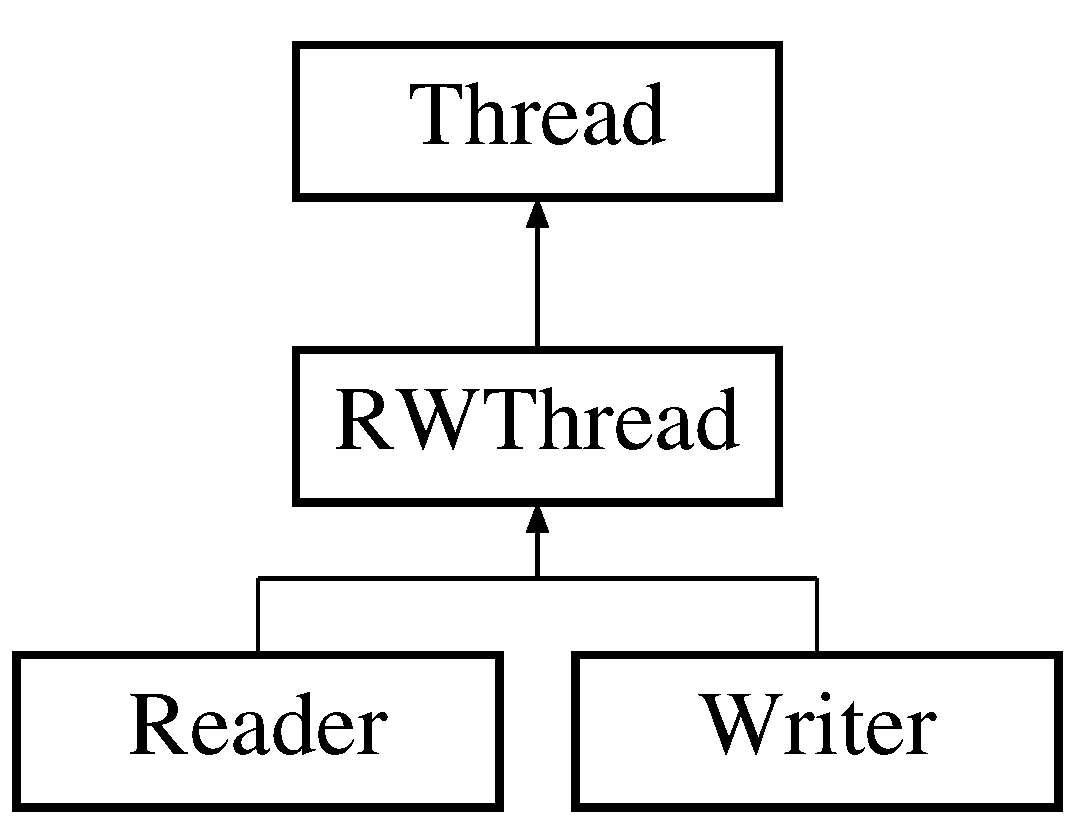
\includegraphics[height=3.000000cm]{class_r_w_thread}
\end{center}
\end{figure}
\subsection*{Public Member Functions}
\begin{DoxyCompactItemize}
\item 
\hyperlink{class_r_w_thread_aa69e6643625bba0aefa86d58cd308827}{R\+W\+Thread} ()
\begin{DoxyCompactList}\small\item\em Default-\/constructor for the \hyperlink{class_r_w_thread}{R\+W\+Thread} class. \end{DoxyCompactList}\item 
\hyperlink{class_r_w_thread_a907cf42de1454ec96ec5620114046f92}{R\+W\+Thread} (\hyperlink{class_r_w_database}{R\+W\+Database}$<$ \hyperlink{classtsgl_1_1_rectangle}{Rectangle} $\ast$$>$ \&shared\+Database, \hyperlink{class_lock}{Lock} \&lock, unsigned long id, \hyperlink{classtsgl_1_1_canvas}{Canvas} \&can)
\begin{DoxyCompactList}\small\item\em Explicit-\/constructor for the \hyperlink{class_r_w_thread}{R\+W\+Thread} class. \end{DoxyCompactList}\item 
\mbox{\Hypertarget{class_r_w_thread_adfb9ef73b0fc09b07db6682ea1fde721}\label{class_r_w_thread_adfb9ef73b0fc09b07db6682ea1fde721}} 
void {\bfseries run} ()
\item 
\mbox{\Hypertarget{class_r_w_thread_ac6d96d9953273f79ccaa3ec5fb2ad56b}\label{class_r_w_thread_ac6d96d9953273f79ccaa3ec5fb2ad56b}} 
void {\bfseries wait} ()
\item 
\mbox{\Hypertarget{class_r_w_thread_a59ec4dac8d85e21715081478303c789e}\label{class_r_w_thread_a59ec4dac8d85e21715081478303c789e}} 
virtual void {\bfseries lock} ()=0
\item 
\mbox{\Hypertarget{class_r_w_thread_a5a29f03164040ee9da4591abcd734528}\label{class_r_w_thread_a5a29f03164040ee9da4591abcd734528}} 
virtual void {\bfseries act} ()=0
\item 
\mbox{\Hypertarget{class_r_w_thread_af747d0aafadb9648baa9486fb598366c}\label{class_r_w_thread_af747d0aafadb9648baa9486fb598366c}} 
virtual void {\bfseries unlock} ()=0
\end{DoxyCompactItemize}
\subsection*{Static Public Attributes}
\begin{DoxyCompactItemize}
\item 
\mbox{\Hypertarget{class_r_w_thread_a341f51c32705a4a512e290aafffd2d14}\label{class_r_w_thread_a341f51c32705a4a512e290aafffd2d14}} 
static const int {\bfseries width} = 20
\item 
\mbox{\Hypertarget{class_r_w_thread_a7839c1805f22372e67752cdee6a6663d}\label{class_r_w_thread_a7839c1805f22372e67752cdee6a6663d}} 
static const int {\bfseries dataX} = -\/100
\item 
\mbox{\Hypertarget{class_r_w_thread_a63c00a2e076956ed629012f43d9b4d31}\label{class_r_w_thread_a63c00a2e076956ed629012f43d9b4d31}} 
static const int {\bfseries dataY} = -\/270
\item 
\mbox{\Hypertarget{class_r_w_thread_a4aa23bfbc63fdce50643f6a01aa4e106}\label{class_r_w_thread_a4aa23bfbc63fdce50643f6a01aa4e106}} 
static const int {\bfseries data\+Height} = 600
\item 
\mbox{\Hypertarget{class_r_w_thread_afbb80d77d6834f770220e8c6cea25f10}\label{class_r_w_thread_afbb80d77d6834f770220e8c6cea25f10}} 
static const int {\bfseries data\+Width} = 200
\item 
\mbox{\Hypertarget{class_r_w_thread_ab5e087e0b95345616711ea03d8aa89cb}\label{class_r_w_thread_ab5e087e0b95345616711ea03d8aa89cb}} 
static int {\bfseries W\+A\+I\+T\+\_\+\+M\+IN} = 15
\item 
\mbox{\Hypertarget{class_r_w_thread_a4b9b080b1e9a899e7173dadb9e915d2d}\label{class_r_w_thread_a4b9b080b1e9a899e7173dadb9e915d2d}} 
static int {\bfseries W\+A\+I\+T\+\_\+\+R\+A\+N\+GE} = 40
\item 
\mbox{\Hypertarget{class_r_w_thread_aa2b4739d82f6242c718db5cfe8af064f}\label{class_r_w_thread_aa2b4739d82f6242c718db5cfe8af064f}} 
static float {\bfseries access\+\_\+wait} = 1.\+0
\item 
\mbox{\Hypertarget{class_r_w_thread_acf3c32cba39bd8a59f129cb6b41d62b9}\label{class_r_w_thread_acf3c32cba39bd8a59f129cb6b41d62b9}} 
static atomic$<$ bool $>$ {\bfseries paused}
\end{DoxyCompactItemize}
\subsection*{Protected Attributes}
\begin{DoxyCompactItemize}
\item 
\mbox{\Hypertarget{class_r_w_thread_a040c2e635a0871c60cb33a13f5379566}\label{class_r_w_thread_a040c2e635a0871c60cb33a13f5379566}} 
int {\bfseries myX}
\item 
\mbox{\Hypertarget{class_r_w_thread_a3a4a2a1cffb15e5c4f326fb5e076ab92}\label{class_r_w_thread_a3a4a2a1cffb15e5c4f326fb5e076ab92}} 
int {\bfseries myY}
\item 
\mbox{\Hypertarget{class_r_w_thread_a430c577265e1370f058afc24bf4f4d2e}\label{class_r_w_thread_a430c577265e1370f058afc24bf4f4d2e}} 
int {\bfseries count}
\item 
\mbox{\Hypertarget{class_r_w_thread_ab2deb3d3e1a5f6a0d4fa50e0f9b9e3f4}\label{class_r_w_thread_ab2deb3d3e1a5f6a0d4fa50e0f9b9e3f4}} 
\hyperlink{class_r_w_database}{R\+W\+Database}$<$ \hyperlink{classtsgl_1_1_rectangle}{Rectangle} $\ast$ $>$ $\ast$ {\bfseries data}
\item 
\mbox{\Hypertarget{class_r_w_thread_acefd6251a6c1f5b0b0fba22645fbe1da}\label{class_r_w_thread_acefd6251a6c1f5b0b0fba22645fbe1da}} 
\hyperlink{class_lock}{Lock} $\ast$ {\bfseries monitor}
\item 
\mbox{\Hypertarget{class_r_w_thread_a6be3c61accb2c1fa24b1125382de3a89}\label{class_r_w_thread_a6be3c61accb2c1fa24b1125382de3a89}} 
\hyperlink{classtsgl_1_1_canvas}{Canvas} $\ast$ {\bfseries my\+Can}
\item 
\mbox{\Hypertarget{class_r_w_thread_ab3259ce53de55087518c441716d80b54}\label{class_r_w_thread_ab3259ce53de55087518c441716d80b54}} 
\hyperlink{classtsgl_1_1_circle}{Circle} $\ast$ {\bfseries my\+Circle}
\item 
\mbox{\Hypertarget{class_r_w_thread_a8edb254652c7f05b2da8c22d7f73919c}\label{class_r_w_thread_a8edb254652c7f05b2da8c22d7f73919c}} 
\hyperlink{classtsgl_1_1_text}{Text} $\ast$ {\bfseries my\+Count\+Label}
\end{DoxyCompactItemize}
\subsection*{Static Protected Attributes}
\begin{DoxyCompactItemize}
\item 
\mbox{\Hypertarget{class_r_w_thread_a19724fd58e85c84f05af0fb4e422a44d}\label{class_r_w_thread_a19724fd58e85c84f05af0fb4e422a44d}} 
static int {\bfseries thread\+Count} = 0
\end{DoxyCompactItemize}
\subsection*{Additional Inherited Members}


\subsection{Detailed Description}
\hyperlink{class_r_w_thread}{R\+W\+Thread} class inherits from the \hyperlink{class_thread}{Thread} class in order to create a \hyperlink{class_r_w_thread}{R\+W\+Thread} object. Inheritance\+: \hyperlink{class_thread}{Thread} class. 

\subsection{Constructor \& Destructor Documentation}
\mbox{\Hypertarget{class_r_w_thread_aa69e6643625bba0aefa86d58cd308827}\label{class_r_w_thread_aa69e6643625bba0aefa86d58cd308827}} 
\index{R\+W\+Thread@{R\+W\+Thread}!R\+W\+Thread@{R\+W\+Thread}}
\index{R\+W\+Thread@{R\+W\+Thread}!R\+W\+Thread@{R\+W\+Thread}}
\subsubsection{\texorpdfstring{R\+W\+Thread()}{RWThread()}\hspace{0.1cm}{\footnotesize\ttfamily [1/2]}}
{\footnotesize\ttfamily R\+W\+Thread\+::\+R\+W\+Thread (\begin{DoxyParamCaption}{ }\end{DoxyParamCaption})}



Default-\/constructor for the \hyperlink{class_r_w_thread}{R\+W\+Thread} class. 

\begin{DoxyReturn}{Returns}
\+: The constructed \hyperlink{class_r_w_thread}{R\+W\+Thread} object. 
\end{DoxyReturn}
\mbox{\Hypertarget{class_r_w_thread_a907cf42de1454ec96ec5620114046f92}\label{class_r_w_thread_a907cf42de1454ec96ec5620114046f92}} 
\index{R\+W\+Thread@{R\+W\+Thread}!R\+W\+Thread@{R\+W\+Thread}}
\index{R\+W\+Thread@{R\+W\+Thread}!R\+W\+Thread@{R\+W\+Thread}}
\subsubsection{\texorpdfstring{R\+W\+Thread()}{RWThread()}\hspace{0.1cm}{\footnotesize\ttfamily [2/2]}}
{\footnotesize\ttfamily R\+W\+Thread\+::\+R\+W\+Thread (\begin{DoxyParamCaption}\item[{\hyperlink{class_r_w_database}{R\+W\+Database}$<$ \hyperlink{classtsgl_1_1_rectangle}{Rectangle} $\ast$$>$ \&}]{shared\+Database,  }\item[{\hyperlink{class_lock}{Lock} \&}]{lock,  }\item[{unsigned long}]{id,  }\item[{\hyperlink{classtsgl_1_1_canvas}{Canvas} \&}]{can }\end{DoxyParamCaption})}



Explicit-\/constructor for the \hyperlink{class_r_w_thread}{R\+W\+Thread} class. 


\begin{DoxyParams}{Parameters}
{\em } & \\
\hline
\end{DoxyParams}


The documentation for this class was generated from the following files\+:\begin{DoxyCompactItemize}
\item 
/home/sth5/test/\+T\+S\+G\+L/src/examples/\+Reader\+Writer/R\+W\+Thread.\+h\item 
/home/sth5/test/\+T\+S\+G\+L/src/examples/\+Reader\+Writer/R\+W\+Thread.\+cpp\end{DoxyCompactItemize}

\hypertarget{class_sea_urchin}{}\section{Sea\+Urchin Class Reference}
\label{class_sea_urchin}\index{Sea\+Urchin@{Sea\+Urchin}}


Who doesn\textquotesingle{}t love sea urchins?  




{\ttfamily \#include $<$Sea\+Urchin.\+h$>$}

\subsection*{Public Member Functions}
\begin{DoxyCompactItemize}
\item 
\hyperlink{class_sea_urchin_a29fac511aa0967424cbfb0729ce06f2c}{Sea\+Urchin} (\hyperlink{classtsgl_1_1_canvas}{Canvas} \&can, int thread\+Id)
\begin{DoxyCompactList}\small\item\em Explicitly construct a \hyperlink{class_sea_urchin}{Sea\+Urchin} object. \end{DoxyCompactList}\item 
void \hyperlink{class_sea_urchin_aa0e038a0faecaead5928edc082dbc685}{move} (\hyperlink{classtsgl_1_1_canvas}{Canvas} \&can)
\begin{DoxyCompactList}\small\item\em Draw the \hyperlink{class_sea_urchin}{Sea\+Urchin}. \end{DoxyCompactList}\item 
virtual \hyperlink{class_sea_urchin_a30d580184797c2cf2b6f6eac21bc3b07}{$\sim$\+Sea\+Urchin} ()
\begin{DoxyCompactList}\small\item\em Destroy a \hyperlink{class_sea_urchin}{Sea\+Urchin}. \end{DoxyCompactList}\end{DoxyCompactItemize}


\subsection{Detailed Description}
Who doesn\textquotesingle{}t love sea urchins? 

Draws a sea urchin onto the Canvas.

Used as an example of what it means to put a process on a thread.

The \hyperlink{class_sea_urchin}{Sea\+Urchin} objects are created in a parallel block, and each thread gets one \hyperlink{class_sea_urchin}{Sea\+Urchin}.

Then, the thread draws the \hyperlink{class_sea_urchin}{Sea\+Urchin} onto the Canvas.

Each \hyperlink{class_sea_urchin}{Sea\+Urchin} object has its own color and plot data based off of the thread\textquotesingle{}s id number.

\hyperlink{class_sea_urchin}{Sea\+Urchin} objects are drawn similar to the line fan in test\+Line\+Fan. \begin{DoxySeeAlso}{See also}
test\+Line\+Fan. 
\end{DoxySeeAlso}


\subsection{Constructor \& Destructor Documentation}
\mbox{\Hypertarget{class_sea_urchin_a29fac511aa0967424cbfb0729ce06f2c}\label{class_sea_urchin_a29fac511aa0967424cbfb0729ce06f2c}} 
\index{Sea\+Urchin@{Sea\+Urchin}!Sea\+Urchin@{Sea\+Urchin}}
\index{Sea\+Urchin@{Sea\+Urchin}!Sea\+Urchin@{Sea\+Urchin}}
\subsubsection{\texorpdfstring{Sea\+Urchin()}{SeaUrchin()}}
{\footnotesize\ttfamily Sea\+Urchin\+::\+Sea\+Urchin (\begin{DoxyParamCaption}\item[{\hyperlink{classtsgl_1_1_canvas}{Canvas} \&}]{can,  }\item[{int}]{thread\+Id }\end{DoxyParamCaption})}



Explicitly construct a \hyperlink{class_sea_urchin}{Sea\+Urchin} object. 

Explicit constructor for a \hyperlink{class_sea_urchin}{Sea\+Urchin} object. 
\begin{DoxyParams}{Parameters}
{\em can} & Reference to the Canvas to draw to. \\
\hline
{\em thread\+Id} & The id of the thread that is currently creating a \hyperlink{class_sea_urchin}{Sea\+Urchin} object. \\
\hline
\end{DoxyParams}
\begin{DoxyReturn}{Returns}
The constructed \hyperlink{class_sea_urchin}{Sea\+Urchin} object. 
\end{DoxyReturn}
\mbox{\Hypertarget{class_sea_urchin_a30d580184797c2cf2b6f6eac21bc3b07}\label{class_sea_urchin_a30d580184797c2cf2b6f6eac21bc3b07}} 
\index{Sea\+Urchin@{Sea\+Urchin}!````~Sea\+Urchin@{$\sim$\+Sea\+Urchin}}
\index{````~Sea\+Urchin@{$\sim$\+Sea\+Urchin}!Sea\+Urchin@{Sea\+Urchin}}
\subsubsection{\texorpdfstring{$\sim$\+Sea\+Urchin()}{~SeaUrchin()}}
{\footnotesize\ttfamily Sea\+Urchin\+::$\sim$\+Sea\+Urchin (\begin{DoxyParamCaption}{ }\end{DoxyParamCaption})\hspace{0.3cm}{\ttfamily [virtual]}}



Destroy a \hyperlink{class_sea_urchin}{Sea\+Urchin}. 

Destructor for a \hyperlink{class_sea_urchin}{Sea\+Urchin} object. \begin{DoxyNote}{Note}
This function does absolutely nothing. 
\end{DoxyNote}


\subsection{Member Function Documentation}
\mbox{\Hypertarget{class_sea_urchin_aa0e038a0faecaead5928edc082dbc685}\label{class_sea_urchin_aa0e038a0faecaead5928edc082dbc685}} 
\index{Sea\+Urchin@{Sea\+Urchin}!move@{move}}
\index{move@{move}!Sea\+Urchin@{Sea\+Urchin}}
\subsubsection{\texorpdfstring{move()}{move()}}
{\footnotesize\ttfamily void Sea\+Urchin\+::move (\begin{DoxyParamCaption}\item[{\hyperlink{classtsgl_1_1_canvas}{Canvas} \&}]{can }\end{DoxyParamCaption})}



Draw the \hyperlink{class_sea_urchin}{Sea\+Urchin}. 

Actually draws the \hyperlink{class_sea_urchin}{Sea\+Urchin} object onto the Canvas. 
\begin{DoxyParams}{Parameters}
{\em can} & Reference to the Canvas object to draw to. \\
\hline
\end{DoxyParams}


The documentation for this class was generated from the following files\+:\begin{DoxyCompactItemize}
\item 
/home/sth5/test/\+T\+S\+G\+L/src/examples/\+Sea\+Urchin/Sea\+Urchin.\+h\item 
/home/sth5/test/\+T\+S\+G\+L/src/examples/\+Sea\+Urchin/Sea\+Urchin.\+cpp\end{DoxyCompactItemize}

\hypertarget{class_shaded_voronoi}{}\section{Shaded\+Voronoi Class Reference}
\label{class_shaded_voronoi}\index{Shaded\+Voronoi@{Shaded\+Voronoi}}


\hyperlink{class_voronoi}{Voronoi} diagram, only shaded!  




{\ttfamily \#include $<$Shaded\+Voronoi.\+h$>$}

Inheritance diagram for Shaded\+Voronoi\+:\begin{figure}[H]
\begin{center}
\leavevmode
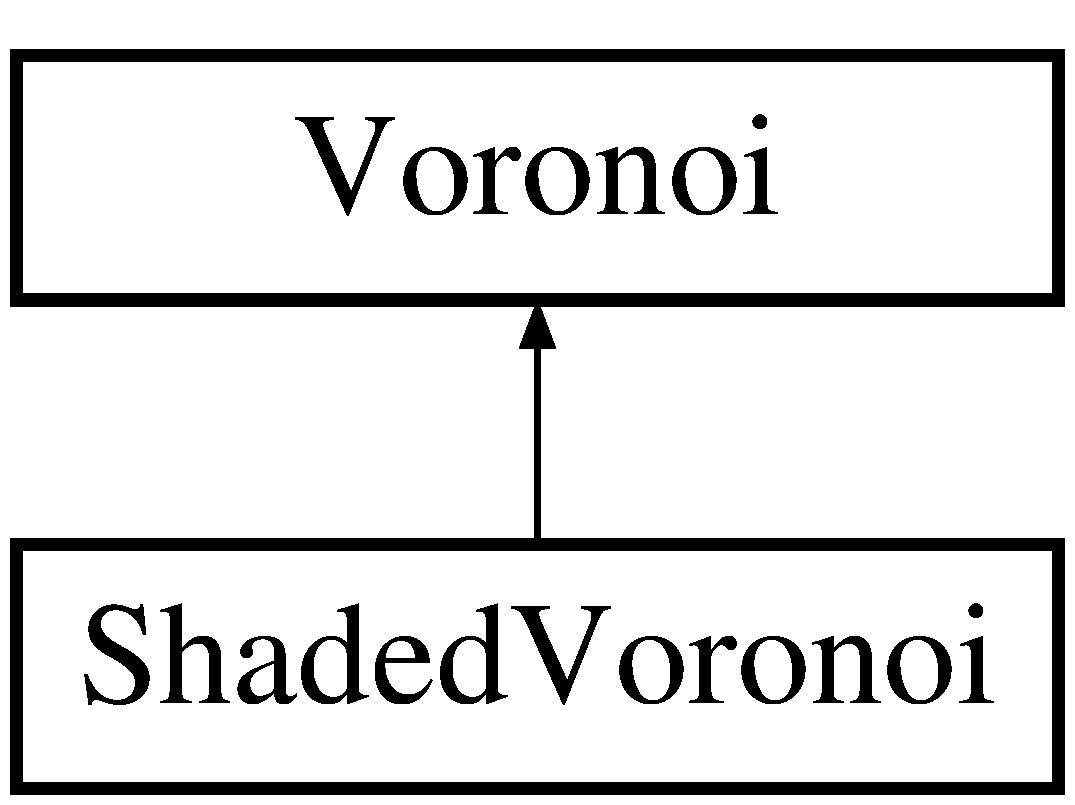
\includegraphics[height=2.000000cm]{class_shaded_voronoi}
\end{center}
\end{figure}
\subsection*{Public Member Functions}
\begin{DoxyCompactItemize}
\item 
\hyperlink{class_shaded_voronoi_a3005ac828c9b8cd099e369c89775c9c9}{Shaded\+Voronoi} (\hyperlink{classtsgl_1_1_canvas}{Canvas} \&can)
\begin{DoxyCompactList}\small\item\em Explicitly construct a \hyperlink{class_shaded_voronoi}{Shaded\+Voronoi} object. \end{DoxyCompactList}\item 
void \hyperlink{class_shaded_voronoi_a5946cbfff9ea57f504cba8235ba814be}{draw} (\hyperlink{classtsgl_1_1_canvas}{Canvas} \&can)
\begin{DoxyCompactList}\small\item\em Draw the \hyperlink{class_shaded_voronoi}{Shaded\+Voronoi} object. \end{DoxyCompactList}\item 
virtual \hyperlink{class_shaded_voronoi_a7f006a50875f62677e209763b6ae2709}{$\sim$\+Shaded\+Voronoi} ()
\begin{DoxyCompactList}\small\item\em Destroy a \hyperlink{class_shaded_voronoi}{Shaded\+Voronoi} object. \end{DoxyCompactList}\end{DoxyCompactItemize}
\subsection*{Additional Inherited Members}


\subsection{Detailed Description}
\hyperlink{class_voronoi}{Voronoi} diagram, only shaded! 

Creates a Shaded \hyperlink{class_voronoi}{Voronoi} diagram.

Similar to a \hyperlink{class_voronoi}{Voronoi} diagram, but with some parts shaded in.

Subclass of the \hyperlink{class_voronoi}{Voronoi} class. \begin{DoxySeeAlso}{See also}
\hyperlink{class_voronoi}{Voronoi} class. 
\end{DoxySeeAlso}


\subsection{Constructor \& Destructor Documentation}
\mbox{\Hypertarget{class_shaded_voronoi_a3005ac828c9b8cd099e369c89775c9c9}\label{class_shaded_voronoi_a3005ac828c9b8cd099e369c89775c9c9}} 
\index{Shaded\+Voronoi@{Shaded\+Voronoi}!Shaded\+Voronoi@{Shaded\+Voronoi}}
\index{Shaded\+Voronoi@{Shaded\+Voronoi}!Shaded\+Voronoi@{Shaded\+Voronoi}}
\subsubsection{\texorpdfstring{Shaded\+Voronoi()}{ShadedVoronoi()}}
{\footnotesize\ttfamily Shaded\+Voronoi\+::\+Shaded\+Voronoi (\begin{DoxyParamCaption}\item[{\hyperlink{classtsgl_1_1_canvas}{Canvas} \&}]{can }\end{DoxyParamCaption})}



Explicitly construct a \hyperlink{class_shaded_voronoi}{Shaded\+Voronoi} object. 

Explicit constructor for a \hyperlink{class_shaded_voronoi}{Shaded\+Voronoi} object. 
\begin{DoxyParams}{Parameters}
{\em can} & Reference to the Canvas to draw to. \\
\hline
\end{DoxyParams}
\begin{DoxyReturn}{Returns}
The constructed \hyperlink{class_shaded_voronoi}{Shaded\+Voronoi} object. 
\end{DoxyReturn}
\mbox{\Hypertarget{class_shaded_voronoi_a7f006a50875f62677e209763b6ae2709}\label{class_shaded_voronoi_a7f006a50875f62677e209763b6ae2709}} 
\index{Shaded\+Voronoi@{Shaded\+Voronoi}!````~Shaded\+Voronoi@{$\sim$\+Shaded\+Voronoi}}
\index{````~Shaded\+Voronoi@{$\sim$\+Shaded\+Voronoi}!Shaded\+Voronoi@{Shaded\+Voronoi}}
\subsubsection{\texorpdfstring{$\sim$\+Shaded\+Voronoi()}{~ShadedVoronoi()}}
{\footnotesize\ttfamily Shaded\+Voronoi\+::$\sim$\+Shaded\+Voronoi (\begin{DoxyParamCaption}{ }\end{DoxyParamCaption})\hspace{0.3cm}{\ttfamily [virtual]}}



Destroy a \hyperlink{class_shaded_voronoi}{Shaded\+Voronoi} object. 

Destructor for a \hyperlink{class_shaded_voronoi}{Shaded\+Voronoi} object. \begin{DoxyReturn}{Returns}
The memory allocated to a \hyperlink{class_shaded_voronoi}{Shaded\+Voronoi} object. 
\end{DoxyReturn}


\subsection{Member Function Documentation}
\mbox{\Hypertarget{class_shaded_voronoi_a5946cbfff9ea57f504cba8235ba814be}\label{class_shaded_voronoi_a5946cbfff9ea57f504cba8235ba814be}} 
\index{Shaded\+Voronoi@{Shaded\+Voronoi}!draw@{draw}}
\index{draw@{draw}!Shaded\+Voronoi@{Shaded\+Voronoi}}
\subsubsection{\texorpdfstring{draw()}{draw()}}
{\footnotesize\ttfamily void Shaded\+Voronoi\+::draw (\begin{DoxyParamCaption}\item[{\hyperlink{classtsgl_1_1_canvas}{Canvas} \&}]{can }\end{DoxyParamCaption})}



Draw the \hyperlink{class_shaded_voronoi}{Shaded\+Voronoi} object. 

Actually draws the \hyperlink{class_shaded_voronoi}{Shaded\+Voronoi} object onto the Canvas. 
\begin{DoxyParams}{Parameters}
{\em can} & Reference to the Canvas to draw to. \\
\hline
\end{DoxyParams}


The documentation for this class was generated from the following files\+:\begin{DoxyCompactItemize}
\item 
/home/sth5/test/\+T\+S\+G\+L/src/examples/\+Voronoi/Shaded\+Voronoi.\+h\item 
/home/sth5/test/\+T\+S\+G\+L/src/examples/\+Voronoi/Shaded\+Voronoi.\+cpp\end{DoxyCompactItemize}

\hypertarget{classtsgl_1_1_shape}{}\section{tsgl\+:\+:Shape Class Reference}
\label{classtsgl_1_1_shape}\index{tsgl\+::\+Shape@{tsgl\+::\+Shape}}


A class for drawing shapes onto a \hyperlink{classtsgl_1_1_canvas}{Canvas} or \hyperlink{classtsgl_1_1_cartesian_canvas}{Cartesian\+Canvas}.  




{\ttfamily \#include $<$Shape.\+h$>$}

Inheritance diagram for tsgl\+:\+:Shape\+:\begin{figure}[H]
\begin{center}
\leavevmode
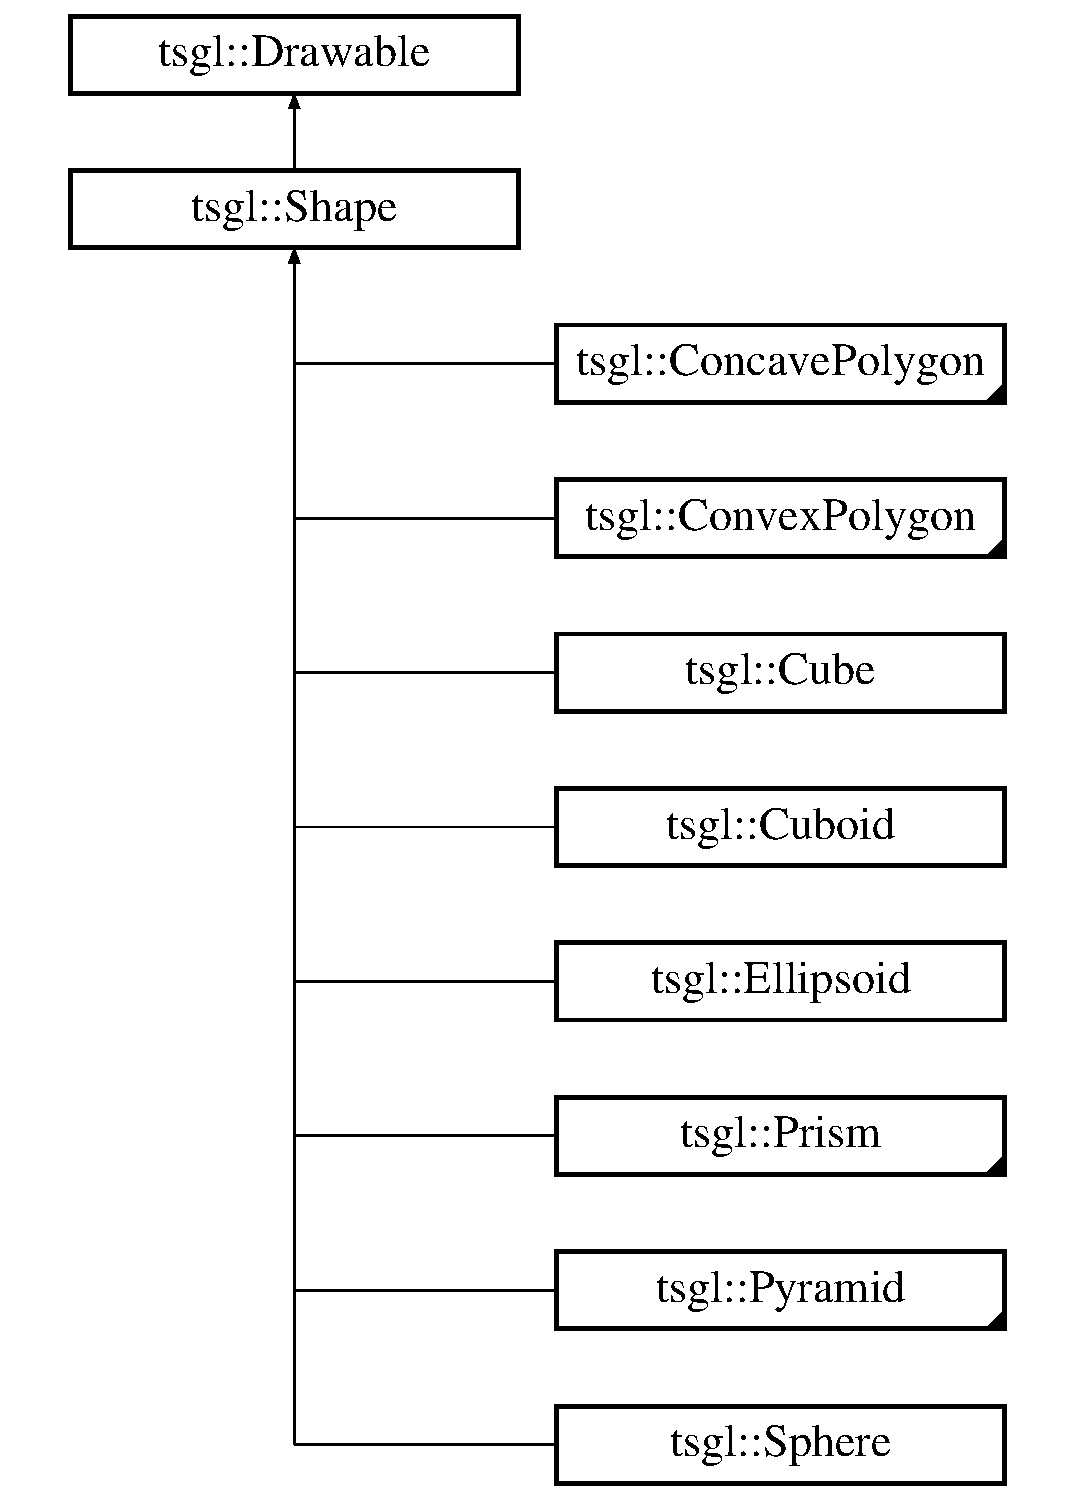
\includegraphics[height=10.000000cm]{classtsgl_1_1_shape}
\end{center}
\end{figure}
\subsection*{Public Member Functions}
\begin{DoxyCompactItemize}
\item 
\hyperlink{classtsgl_1_1_shape_a2e6d954b348471650b72d8e0519288ed}{Shape} (float x, float y, float z, float yaw, float pitch, float roll)
\begin{DoxyCompactList}\small\item\em Constructs a new \hyperlink{classtsgl_1_1_shape}{Shape}. \end{DoxyCompactList}\item 
virtual void \hyperlink{classtsgl_1_1_shape_ae0905e73f1652d92cef9c7f2c38572f3}{draw} (Shader $\ast$shader)
\begin{DoxyCompactList}\small\item\em Draw the \hyperlink{classtsgl_1_1_shape}{Shape}. \end{DoxyCompactList}\item 
virtual void \hyperlink{classtsgl_1_1_shape_abdb01321cddfd2db1481eefbc2836f70}{set\+Color} (\hyperlink{structtsgl_1_1_color_float}{Color\+Float} c)
\begin{DoxyCompactList}\small\item\em Sets the \hyperlink{classtsgl_1_1_shape}{Shape} to a new color. \end{DoxyCompactList}\item 
virtual void \hyperlink{classtsgl_1_1_shape_ad7e554b5d4cea111ec518548b9f21388}{set\+Color} (\hyperlink{structtsgl_1_1_color_float}{Color\+Float} c\mbox{[}$\,$\mbox{]})
\begin{DoxyCompactList}\small\item\em Sets the \hyperlink{classtsgl_1_1_shape}{Shape} to a new array of colors. \end{DoxyCompactList}\item 
virtual void \hyperlink{classtsgl_1_1_shape_a30a5a08919f22700ad96ec84de033864}{set\+Outline\+Color} (\hyperlink{structtsgl_1_1_color_float}{Color\+Float} c)
\begin{DoxyCompactList}\small\item\em Sets the \hyperlink{classtsgl_1_1_shape}{Shape}\textquotesingle{}s outline to a new color. \end{DoxyCompactList}\item 
virtual \hyperlink{structtsgl_1_1_color_float}{Color\+Float} \hyperlink{classtsgl_1_1_shape_ab531d3d4ddca94ec14ec29f381eab838}{get\+Color} ()
\begin{DoxyCompactList}\small\item\em Accessor for \hyperlink{classtsgl_1_1_shape}{Shape}\textquotesingle{}s color. \end{DoxyCompactList}\item 
virtual void \hyperlink{classtsgl_1_1_shape_a6f54fe4d049f69a287edf8335a9509f8}{get\+Colors} (std\+::vector$<$ \hyperlink{structtsgl_1_1_color_float}{Color\+Float} $>$ \&color\+Vec)
\begin{DoxyCompactList}\small\item\em Accessor for \hyperlink{classtsgl_1_1_shape}{Shape}\textquotesingle{}s colors. \end{DoxyCompactList}\item 
virtual bool \hyperlink{classtsgl_1_1_shape_adf7724c786882b2bd4375c1e4807ed5d}{is\+Processed} ()
\begin{DoxyCompactList}\small\item\em Accessor that returns if \hyperlink{classtsgl_1_1_drawable}{Drawable} is processed and ready to be drawn. \end{DoxyCompactList}\item 
virtual void \hyperlink{classtsgl_1_1_shape_acf10e14a8b26ced8926fcdeaf42e8728}{set\+Is\+Filled} (bool status)
\begin{DoxyCompactList}\small\item\em Set whether or not the \hyperlink{classtsgl_1_1_shape}{Shape} will be filled. \end{DoxyCompactList}\item 
virtual void \hyperlink{classtsgl_1_1_shape_afedf4a424c24ed38c389f09cd5ecf451}{set\+Is\+Outlined} (bool status)
\begin{DoxyCompactList}\small\item\em Set whether or not the \hyperlink{classtsgl_1_1_shape}{Shape} will be outlined. \end{DoxyCompactList}\end{DoxyCompactItemize}
\subsection*{Protected Member Functions}
\begin{DoxyCompactItemize}
\item 
virtual void \hyperlink{classtsgl_1_1_shape_ac0ea13ecde43ce62262f82597fb94755}{add\+Vertex} (G\+Lfloat x, G\+Lfloat y, G\+Lfloat z, const \hyperlink{structtsgl_1_1_color_float}{Color\+Float} \&color=W\+H\+I\+TE)
\begin{DoxyCompactList}\small\item\em Adds another vertex to a \hyperlink{classtsgl_1_1_shape}{Shape}. \end{DoxyCompactList}\item 
virtual void \hyperlink{classtsgl_1_1_shape_aeb780a6a509ccceae2323508745cd8fd}{add\+Outline\+Vertex} (G\+Lfloat x, G\+Lfloat y, G\+Lfloat z, const \hyperlink{structtsgl_1_1_color_float}{Color\+Float} \&color=W\+H\+I\+TE)
\begin{DoxyCompactList}\small\item\em Adds another outline vertex to a \hyperlink{classtsgl_1_1_shape}{Shape}. \end{DoxyCompactList}\end{DoxyCompactItemize}
\subsection*{Protected Attributes}
\begin{DoxyCompactItemize}
\item 
\mbox{\Hypertarget{classtsgl_1_1_shape_a655e9c7ff27f80cad1baf807b17ee1f3}\label{classtsgl_1_1_shape_a655e9c7ff27f80cad1baf807b17ee1f3}} 
int {\bfseries number\+Of\+Vertices}
\item 
\mbox{\Hypertarget{classtsgl_1_1_shape_ac20c1a30c7b69386760e676e51df4f03}\label{classtsgl_1_1_shape_ac20c1a30c7b69386760e676e51df4f03}} 
int {\bfseries current\+Vertex} = 0
\item 
\mbox{\Hypertarget{classtsgl_1_1_shape_a5d604679fb7fe7642e3c939b9c0d9878}\label{classtsgl_1_1_shape_a5d604679fb7fe7642e3c939b9c0d9878}} 
G\+Lenum {\bfseries geometry\+Type}
\item 
\mbox{\Hypertarget{classtsgl_1_1_shape_ae8f28c1fbfae15550e21afad5d2f8efb}\label{classtsgl_1_1_shape_ae8f28c1fbfae15550e21afad5d2f8efb}} 
bool {\bfseries is\+Filled} = true
\item 
\mbox{\Hypertarget{classtsgl_1_1_shape_a272bb594b2a88973184508106033362a}\label{classtsgl_1_1_shape_a272bb594b2a88973184508106033362a}} 
int {\bfseries number\+Of\+Outline\+Vertices}
\item 
\mbox{\Hypertarget{classtsgl_1_1_shape_a958bab81b4fba5437233b63a6da5d0ec}\label{classtsgl_1_1_shape_a958bab81b4fba5437233b63a6da5d0ec}} 
int {\bfseries current\+Outline\+Vertex} = 0
\item 
\mbox{\Hypertarget{classtsgl_1_1_shape_ad28dc9ae636185561290014f8036fd52}\label{classtsgl_1_1_shape_ad28dc9ae636185561290014f8036fd52}} 
G\+Lenum {\bfseries outline\+Geometry\+Type}
\item 
\mbox{\Hypertarget{classtsgl_1_1_shape_a0c885ba3f3311a8cbc48dd68bb0fda86}\label{classtsgl_1_1_shape_a0c885ba3f3311a8cbc48dd68bb0fda86}} 
G\+Lfloat $\ast$ {\bfseries outline\+Vertices}
\item 
\mbox{\Hypertarget{classtsgl_1_1_shape_ab497c48cdfd680525f3b3cc2704619e8}\label{classtsgl_1_1_shape_ab497c48cdfd680525f3b3cc2704619e8}} 
bool {\bfseries is\+Outlined} = true
\item 
\mbox{\Hypertarget{classtsgl_1_1_shape_a6a2f21a402a717d48eaeeee36b6228ae}\label{classtsgl_1_1_shape_a6a2f21a402a717d48eaeeee36b6228ae}} 
bool {\bfseries outline\+Init} = false
\end{DoxyCompactItemize}


\subsection{Detailed Description}
A class for drawing shapes onto a \hyperlink{classtsgl_1_1_canvas}{Canvas} or \hyperlink{classtsgl_1_1_cartesian_canvas}{Cartesian\+Canvas}. 

\begin{DoxyWarning}{Warning}
{\bfseries {\itshape Though extending this class must be allowed due to the way the code is set up, attempting to do so could potentially mess up the internal GL calls the library uses. Proceed with great caution.}}
\end{DoxyWarning}
\hyperlink{classtsgl_1_1_shape}{Shape} provides a base class for drawing shapes to a \hyperlink{classtsgl_1_1_canvas}{Canvas} or \hyperlink{classtsgl_1_1_cartesian_canvas}{Cartesian\+Canvas}. \begin{DoxyNote}{Note}
\hyperlink{classtsgl_1_1_shape}{Shape} is abstract, and must be extended by the user.
\end{DoxyNote}
{\ttfamily vertices} should be an array of floating point values in T\+S\+GL\textquotesingle{}s vertex format. One vertex consists of 6 floating point values, signifying x,y,red,green,blue,and alpha components respectively. E.\+g., to draw a triangle, you would need 3 vertices = 18 floats -\/$>$ vertices should be an array of length 18.

{\ttfamily numberofvertices} should be the actual integer number of vertices to be drawn (e.\+g., {\itshape 3} for a triangle).

{\ttfamily drawingmode} should be one of GL\textquotesingle{}s primitive drawing modes. See \href{https://www.opengl.org/sdk/docs/man2/xhtml/glBegin.xml}{\tt https\+://www.\+opengl.\+org/sdk/docs/man2/xhtml/gl\+Begin.\+xml} for further information.

Theoretically, you could potentially extend the \hyperlink{classtsgl_1_1_shape}{Shape} class so that you can create another \hyperlink{classtsgl_1_1_shape}{Shape} class that suits your needs.

However, this is not recommended for normal use of the T\+S\+GL library. 

\subsection{Constructor \& Destructor Documentation}
\mbox{\Hypertarget{classtsgl_1_1_shape_a2e6d954b348471650b72d8e0519288ed}\label{classtsgl_1_1_shape_a2e6d954b348471650b72d8e0519288ed}} 
\index{tsgl\+::\+Shape@{tsgl\+::\+Shape}!Shape@{Shape}}
\index{Shape@{Shape}!tsgl\+::\+Shape@{tsgl\+::\+Shape}}
\subsubsection{\texorpdfstring{Shape()}{Shape()}}
{\footnotesize\ttfamily tsgl\+::\+Shape\+::\+Shape (\begin{DoxyParamCaption}\item[{float}]{x,  }\item[{float}]{y,  }\item[{float}]{z,  }\item[{float}]{yaw,  }\item[{float}]{pitch,  }\item[{float}]{roll }\end{DoxyParamCaption})}



Constructs a new \hyperlink{classtsgl_1_1_shape}{Shape}. 


\begin{DoxyItemize}
\item Usually {\ttfamily vertices} is filled with floating point values that represent the vertices of the shape to be drawn.
\item You may define other items in the constructor that pertain to the attributes of the subclass that is extending \hyperlink{classtsgl_1_1_shape}{Shape}.
\item At a minimum, you {\itshape M\+U\+ST} fill an array of floating point values that pertain to the vertices of the shape. \begin{DoxyWarning}{Warning}
{\bfseries You {\itshape must} inherit the parent\textquotesingle{}s constructor if you are extending \hyperlink{classtsgl_1_1_shape}{Shape}.} 
\end{DoxyWarning}
\begin{DoxyNote}{Note}
Refer to the \hyperlink{classtsgl_1_1_shape}{Shape} class description for more details. 
\end{DoxyNote}

\end{DoxyItemize}

\subsection{Member Function Documentation}
\mbox{\Hypertarget{classtsgl_1_1_shape_aeb780a6a509ccceae2323508745cd8fd}\label{classtsgl_1_1_shape_aeb780a6a509ccceae2323508745cd8fd}} 
\index{tsgl\+::\+Shape@{tsgl\+::\+Shape}!add\+Outline\+Vertex@{add\+Outline\+Vertex}}
\index{add\+Outline\+Vertex@{add\+Outline\+Vertex}!tsgl\+::\+Shape@{tsgl\+::\+Shape}}
\subsubsection{\texorpdfstring{add\+Outline\+Vertex()}{addOutlineVertex()}}
{\footnotesize\ttfamily void tsgl\+::\+Shape\+::add\+Outline\+Vertex (\begin{DoxyParamCaption}\item[{G\+Lfloat}]{x,  }\item[{G\+Lfloat}]{y,  }\item[{G\+Lfloat}]{z,  }\item[{const \hyperlink{structtsgl_1_1_color_float}{Color\+Float} \&}]{color = {\ttfamily WHITE} }\end{DoxyParamCaption})\hspace{0.3cm}{\ttfamily [protected]}, {\ttfamily [virtual]}}



Adds another outline vertex to a \hyperlink{classtsgl_1_1_shape}{Shape}. 

This function initializes the next vertex in the \hyperlink{classtsgl_1_1_shape}{Shape} and adds it to a \hyperlink{classtsgl_1_1_shape}{Shape} buffer. 
\begin{DoxyParams}{Parameters}
{\em x} & The x position of the vertex. \\
\hline
{\em y} & The y position of the vertex. \\
\hline
{\em z} & The z position of the vertex. \\
\hline
{\em color} & The reference variable of the color of the vertex. \\
\hline
\end{DoxyParams}
\begin{DoxyNote}{Note}
This function does nothing if the vertex buffer is already full. 

A message is given indicating that the vertex buffer is full. 
\end{DoxyNote}


Referenced by tsgl\+::\+Arrow\+::\+Arrow(), tsgl\+::\+Circle\+::\+Circle(), tsgl\+::\+Concave\+Polygon\+::\+Concave\+Polygon(), tsgl\+::\+Convex\+Polygon\+::\+Convex\+Polygon(), tsgl\+::\+Cube\+::\+Cube(), tsgl\+::\+Cuboid\+::\+Cuboid(), tsgl\+::\+Ellipse\+::\+Ellipse(), tsgl\+::\+Ellipsoid\+::\+Ellipsoid(), tsgl\+::\+Prism\+::\+Prism(), tsgl\+::\+Pyramid\+::\+Pyramid(), tsgl\+::\+Rectangle\+::\+Rectangle(), tsgl\+::\+Regular\+Polygon\+::\+Regular\+Polygon(), tsgl\+::\+Sphere\+::\+Sphere(), tsgl\+::\+Square\+::\+Square(), tsgl\+::\+Star\+::\+Star(), tsgl\+::\+Triangle\+::\+Triangle(), and tsgl\+::\+Triangle\+Strip\+::\+Triangle\+Strip().

\mbox{\Hypertarget{classtsgl_1_1_shape_ac0ea13ecde43ce62262f82597fb94755}\label{classtsgl_1_1_shape_ac0ea13ecde43ce62262f82597fb94755}} 
\index{tsgl\+::\+Shape@{tsgl\+::\+Shape}!add\+Vertex@{add\+Vertex}}
\index{add\+Vertex@{add\+Vertex}!tsgl\+::\+Shape@{tsgl\+::\+Shape}}
\subsubsection{\texorpdfstring{add\+Vertex()}{addVertex()}}
{\footnotesize\ttfamily void tsgl\+::\+Shape\+::add\+Vertex (\begin{DoxyParamCaption}\item[{G\+Lfloat}]{x,  }\item[{G\+Lfloat}]{y,  }\item[{G\+Lfloat}]{z,  }\item[{const \hyperlink{structtsgl_1_1_color_float}{Color\+Float} \&}]{color = {\ttfamily WHITE} }\end{DoxyParamCaption})\hspace{0.3cm}{\ttfamily [protected]}, {\ttfamily [virtual]}}



Adds another vertex to a \hyperlink{classtsgl_1_1_shape}{Shape}. 

This function initializes the next vertex in the \hyperlink{classtsgl_1_1_shape}{Shape} and adds it to a \hyperlink{classtsgl_1_1_shape}{Shape} buffer. 
\begin{DoxyParams}{Parameters}
{\em x} & The x position of the vertex. \\
\hline
{\em y} & The y position of the vertex. \\
\hline
{\em z} & The z position of the vertex. \\
\hline
{\em color} & The reference variable of the color of the vertex. \\
\hline
\end{DoxyParams}
\begin{DoxyNote}{Note}
This function does nothing if the vertex buffer is already full. 

A message is given indicating that the vertex buffer is full. 
\end{DoxyNote}


Referenced by tsgl\+::\+Arrow\+::\+Arrow(), tsgl\+::\+Circle\+::\+Circle(), tsgl\+::\+Concave\+Polygon\+::\+Concave\+Polygon(), tsgl\+::\+Convex\+Polygon\+::\+Convex\+Polygon(), tsgl\+::\+Cube\+::\+Cube(), tsgl\+::\+Cuboid\+::\+Cuboid(), tsgl\+::\+Ellipse\+::\+Ellipse(), tsgl\+::\+Ellipsoid\+::\+Ellipsoid(), tsgl\+::\+Prism\+::\+Prism(), tsgl\+::\+Pyramid\+::\+Pyramid(), tsgl\+::\+Rectangle\+::\+Rectangle(), tsgl\+::\+Regular\+Polygon\+::\+Regular\+Polygon(), tsgl\+::\+Sphere\+::\+Sphere(), tsgl\+::\+Square\+::\+Square(), tsgl\+::\+Star\+::\+Star(), tsgl\+::\+Triangle\+::\+Triangle(), and tsgl\+::\+Triangle\+Strip\+::\+Triangle\+Strip().

\mbox{\Hypertarget{classtsgl_1_1_shape_ae0905e73f1652d92cef9c7f2c38572f3}\label{classtsgl_1_1_shape_ae0905e73f1652d92cef9c7f2c38572f3}} 
\index{tsgl\+::\+Shape@{tsgl\+::\+Shape}!draw@{draw}}
\index{draw@{draw}!tsgl\+::\+Shape@{tsgl\+::\+Shape}}
\subsubsection{\texorpdfstring{draw()}{draw()}}
{\footnotesize\ttfamily void tsgl\+::\+Shape\+::draw (\begin{DoxyParamCaption}\item[{Shader $\ast$}]{shader }\end{DoxyParamCaption})\hspace{0.3cm}{\ttfamily [virtual]}}



Draw the \hyperlink{classtsgl_1_1_shape}{Shape}. 

This function actually draws the \hyperlink{classtsgl_1_1_shape}{Shape} to the \hyperlink{classtsgl_1_1_canvas}{Canvas}. \begin{DoxyNote}{Note}
This function does nothing if the vertex buffer is not yet full. 

A message indicating that the \hyperlink{classtsgl_1_1_shape}{Shape} cannot be drawn yet will be given if the above condition is met (vertex buffer = not full). 
\end{DoxyNote}


Implements \hyperlink{classtsgl_1_1_drawable}{tsgl\+::\+Drawable}.



Reimplemented in \hyperlink{classtsgl_1_1_concave_polygon_adf288a6b60873a7ae5e599f63868da82}{tsgl\+::\+Concave\+Polygon}.



Referenced by tsgl\+::\+Progress\+Bar\+::$\sim$\+Progress\+Bar().

\mbox{\Hypertarget{classtsgl_1_1_shape_ab531d3d4ddca94ec14ec29f381eab838}\label{classtsgl_1_1_shape_ab531d3d4ddca94ec14ec29f381eab838}} 
\index{tsgl\+::\+Shape@{tsgl\+::\+Shape}!get\+Color@{get\+Color}}
\index{get\+Color@{get\+Color}!tsgl\+::\+Shape@{tsgl\+::\+Shape}}
\subsubsection{\texorpdfstring{get\+Color()}{getColor()}}
{\footnotesize\ttfamily \hyperlink{structtsgl_1_1_color_float}{Color\+Float} tsgl\+::\+Shape\+::get\+Color (\begin{DoxyParamCaption}{ }\end{DoxyParamCaption})\hspace{0.3cm}{\ttfamily [virtual]}}



Accessor for \hyperlink{classtsgl_1_1_shape}{Shape}\textquotesingle{}s color. 

Returns the color of \hyperlink{classtsgl_1_1_shape}{Shape}\textquotesingle{}s first vertex. \begin{DoxyNote}{Note}
For multicolored Shapes, use \hyperlink{classtsgl_1_1_shape_a6f54fe4d049f69a287edf8335a9509f8}{get\+Colors()} to access a vector of all relevant colors. 
\end{DoxyNote}


Referenced by Consumer\+::act(), Reader\+::\+Reader(), Producer\+::wait(), and Writer\+::\+Writer().

\mbox{\Hypertarget{classtsgl_1_1_shape_a6f54fe4d049f69a287edf8335a9509f8}\label{classtsgl_1_1_shape_a6f54fe4d049f69a287edf8335a9509f8}} 
\index{tsgl\+::\+Shape@{tsgl\+::\+Shape}!get\+Colors@{get\+Colors}}
\index{get\+Colors@{get\+Colors}!tsgl\+::\+Shape@{tsgl\+::\+Shape}}
\subsubsection{\texorpdfstring{get\+Colors()}{getColors()}}
{\footnotesize\ttfamily void tsgl\+::\+Shape\+::get\+Colors (\begin{DoxyParamCaption}\item[{std\+::vector$<$ \hyperlink{structtsgl_1_1_color_float}{Color\+Float} $>$ \&}]{color\+Vec }\end{DoxyParamCaption})\hspace{0.3cm}{\ttfamily [virtual]}}



Accessor for \hyperlink{classtsgl_1_1_shape}{Shape}\textquotesingle{}s colors. 

Populates the reference parameter vector with a \hyperlink{structtsgl_1_1_color_float}{Color\+Float} for each vertex of \hyperlink{classtsgl_1_1_shape}{Shape}. 
\begin{DoxyParams}{Parameters}
{\em color\+Vec} & A vector of Color\+Floats to which the Color\+Floats associated with \hyperlink{classtsgl_1_1_shape}{Shape} will be pushed. \\
\hline
\end{DoxyParams}


Reimplemented in \hyperlink{classtsgl_1_1_arrow_a45f13b066c85baae9712730787f49fac}{tsgl\+::\+Arrow}, \hyperlink{classtsgl_1_1_cuboid_ac3e7d161cb2dbb02cf000e92d84e10ba}{tsgl\+::\+Cuboid}, \hyperlink{classtsgl_1_1_prism_abfdc091d8c61e889f61b71577b58e0b6}{tsgl\+::\+Prism}, \hyperlink{classtsgl_1_1_pyramid_a9c93002e90ac1f3385c4d3154ca0321a}{tsgl\+::\+Pyramid}, \hyperlink{classtsgl_1_1_ellipse_a3d92da146589fc58112945daefafe98f}{tsgl\+::\+Ellipse}, \hyperlink{classtsgl_1_1_ellipsoid_ac5c9278659df646c17ef4172e13c7cb3}{tsgl\+::\+Ellipsoid}, \hyperlink{classtsgl_1_1_cube_ac1d31d18439024e4160db369df463a7d}{tsgl\+::\+Cube}, \hyperlink{classtsgl_1_1_circle_af0e1ef7313bde5f66750b616de296f76}{tsgl\+::\+Circle}, and \hyperlink{classtsgl_1_1_sphere_a767bfb1b0c6c29d0577377aa0403d881}{tsgl\+::\+Sphere}.

\mbox{\Hypertarget{classtsgl_1_1_shape_adf7724c786882b2bd4375c1e4807ed5d}\label{classtsgl_1_1_shape_adf7724c786882b2bd4375c1e4807ed5d}} 
\index{tsgl\+::\+Shape@{tsgl\+::\+Shape}!is\+Processed@{is\+Processed}}
\index{is\+Processed@{is\+Processed}!tsgl\+::\+Shape@{tsgl\+::\+Shape}}
\subsubsection{\texorpdfstring{is\+Processed()}{isProcessed()}}
{\footnotesize\ttfamily virtual bool tsgl\+::\+Shape\+::is\+Processed (\begin{DoxyParamCaption}{ }\end{DoxyParamCaption})\hspace{0.3cm}{\ttfamily [inline]}, {\ttfamily [virtual]}}



Accessor that returns if \hyperlink{classtsgl_1_1_drawable}{Drawable} is processed and ready to be drawn. 

This function returns true only if all vertices have been inserted into an array. 

Reimplemented from \hyperlink{classtsgl_1_1_drawable_a98562ec95c8621ba9b46d7bd0c0ffece}{tsgl\+::\+Drawable}.

\mbox{\Hypertarget{classtsgl_1_1_shape_abdb01321cddfd2db1481eefbc2836f70}\label{classtsgl_1_1_shape_abdb01321cddfd2db1481eefbc2836f70}} 
\index{tsgl\+::\+Shape@{tsgl\+::\+Shape}!set\+Color@{set\+Color}}
\index{set\+Color@{set\+Color}!tsgl\+::\+Shape@{tsgl\+::\+Shape}}
\subsubsection{\texorpdfstring{set\+Color()}{setColor()}\hspace{0.1cm}{\footnotesize\ttfamily [1/2]}}
{\footnotesize\ttfamily void tsgl\+::\+Shape\+::set\+Color (\begin{DoxyParamCaption}\item[{\hyperlink{structtsgl_1_1_color_float}{Color\+Float}}]{c }\end{DoxyParamCaption})\hspace{0.3cm}{\ttfamily [virtual]}}



Sets the \hyperlink{classtsgl_1_1_shape}{Shape} to a new color. 


\begin{DoxyParams}{Parameters}
{\em c} & The new \hyperlink{structtsgl_1_1_color_float}{Color\+Float}. \\
\hline
\end{DoxyParams}


Reimplemented in \hyperlink{classtsgl_1_1_arrow_a4eabf87c29f3da697fe39006c45510b7}{tsgl\+::\+Arrow}, \hyperlink{classtsgl_1_1_cuboid_a683f0eeb463e9779e954955f92f12f8e}{tsgl\+::\+Cuboid}, \hyperlink{classtsgl_1_1_prism_af2c681fd9cf74eaede3dd4fd8dd10625}{tsgl\+::\+Prism}, \hyperlink{classtsgl_1_1_pyramid_aef16d8830e2dfac0e8a30d091d099c30}{tsgl\+::\+Pyramid}, \hyperlink{classtsgl_1_1_ellipse_afb71964e56fdd50e49ba46e8090aa858}{tsgl\+::\+Ellipse}, \hyperlink{classtsgl_1_1_ellipsoid_afc2fc98057e5d19d8fa0c45f07273cdb}{tsgl\+::\+Ellipsoid}, \hyperlink{classtsgl_1_1_cube_a4eb42afdc453fa0c768924a26e5cd870}{tsgl\+::\+Cube}, \hyperlink{classtsgl_1_1_circle_a3e97ff653a534a606f0a3b3176c330b0}{tsgl\+::\+Circle}, and \hyperlink{classtsgl_1_1_sphere_aa0870a70e34c6c77e2d61e50dbf3cc07}{tsgl\+::\+Sphere}.



Referenced by Consumer\+::act(), Consumer\+::lock(), Producer\+::lock(), Paddle\+::\+Paddle(), tsgl\+::\+Circle\+::set\+Color(), tsgl\+::\+Cube\+::set\+Color(), tsgl\+::\+Ellipse\+::set\+Color(), tsgl\+::\+Prism\+::set\+Color(), tsgl\+::\+Cuboid\+::set\+Color(), tsgl\+::\+Arrow\+::set\+Color(), Producer\+::wait(), and Writer\+::\+Writer().

\mbox{\Hypertarget{classtsgl_1_1_shape_ad7e554b5d4cea111ec518548b9f21388}\label{classtsgl_1_1_shape_ad7e554b5d4cea111ec518548b9f21388}} 
\index{tsgl\+::\+Shape@{tsgl\+::\+Shape}!set\+Color@{set\+Color}}
\index{set\+Color@{set\+Color}!tsgl\+::\+Shape@{tsgl\+::\+Shape}}
\subsubsection{\texorpdfstring{set\+Color()}{setColor()}\hspace{0.1cm}{\footnotesize\ttfamily [2/2]}}
{\footnotesize\ttfamily void tsgl\+::\+Shape\+::set\+Color (\begin{DoxyParamCaption}\item[{\hyperlink{structtsgl_1_1_color_float}{Color\+Float}}]{c\mbox{[}$\,$\mbox{]} }\end{DoxyParamCaption})\hspace{0.3cm}{\ttfamily [virtual]}}



Sets the \hyperlink{classtsgl_1_1_shape}{Shape} to a new array of colors. 


\begin{DoxyParams}{Parameters}
{\em c} & The new array of Color\+Floats. \\
\hline
\end{DoxyParams}


Reimplemented in \hyperlink{classtsgl_1_1_arrow_a7804a81f8ae4ae0208e80849438364f0}{tsgl\+::\+Arrow}, \hyperlink{classtsgl_1_1_cuboid_aab8a70aff0dcede030ac51277c0dc255}{tsgl\+::\+Cuboid}, \hyperlink{classtsgl_1_1_prism_a668c2779da173493efc0c4634750bd66}{tsgl\+::\+Prism}, \hyperlink{classtsgl_1_1_pyramid_a83799687df3bdef698f9687da7a6c100}{tsgl\+::\+Pyramid}, \hyperlink{classtsgl_1_1_ellipse_a052ef5a609d7e8516d973ddc9e549c89}{tsgl\+::\+Ellipse}, \hyperlink{classtsgl_1_1_ellipsoid_ab8e15e879521e4c96be8192258cad26e}{tsgl\+::\+Ellipsoid}, \hyperlink{classtsgl_1_1_cube_a28111319d350040165bd24d92342c7cc}{tsgl\+::\+Cube}, \hyperlink{classtsgl_1_1_circle_aa25c336d07fb8216bd5d6f63f53a2271}{tsgl\+::\+Circle}, and \hyperlink{classtsgl_1_1_sphere_aab902ab87c24e7065c74f553f7e8c126}{tsgl\+::\+Sphere}.

\mbox{\Hypertarget{classtsgl_1_1_shape_acf10e14a8b26ced8926fcdeaf42e8728}\label{classtsgl_1_1_shape_acf10e14a8b26ced8926fcdeaf42e8728}} 
\index{tsgl\+::\+Shape@{tsgl\+::\+Shape}!set\+Is\+Filled@{set\+Is\+Filled}}
\index{set\+Is\+Filled@{set\+Is\+Filled}!tsgl\+::\+Shape@{tsgl\+::\+Shape}}
\subsubsection{\texorpdfstring{set\+Is\+Filled()}{setIsFilled()}}
{\footnotesize\ttfamily virtual void tsgl\+::\+Shape\+::set\+Is\+Filled (\begin{DoxyParamCaption}\item[{bool}]{status }\end{DoxyParamCaption})\hspace{0.3cm}{\ttfamily [inline]}, {\ttfamily [virtual]}}



Set whether or not the \hyperlink{classtsgl_1_1_shape}{Shape} will be filled. 

Sets the is\+Filled instance variable to the value of the parameter. 
\begin{DoxyParams}{Parameters}
{\em status} & Boolean value to which is\+Filled will be set equivalent. \\
\hline
\end{DoxyParams}
\begin{DoxyWarning}{Warning}
Disabling fill on some 3D Shapes, like \hyperlink{classtsgl_1_1_cone}{Cone} and \hyperlink{classtsgl_1_1_cylinder}{Cylinder}, can be awkward visually. 
\end{DoxyWarning}
\mbox{\Hypertarget{classtsgl_1_1_shape_afedf4a424c24ed38c389f09cd5ecf451}\label{classtsgl_1_1_shape_afedf4a424c24ed38c389f09cd5ecf451}} 
\index{tsgl\+::\+Shape@{tsgl\+::\+Shape}!set\+Is\+Outlined@{set\+Is\+Outlined}}
\index{set\+Is\+Outlined@{set\+Is\+Outlined}!tsgl\+::\+Shape@{tsgl\+::\+Shape}}
\subsubsection{\texorpdfstring{set\+Is\+Outlined()}{setIsOutlined()}}
{\footnotesize\ttfamily virtual void tsgl\+::\+Shape\+::set\+Is\+Outlined (\begin{DoxyParamCaption}\item[{bool}]{status }\end{DoxyParamCaption})\hspace{0.3cm}{\ttfamily [inline]}, {\ttfamily [virtual]}}



Set whether or not the \hyperlink{classtsgl_1_1_shape}{Shape} will be outlined. 

Sets the is\+Outlined instance variable to the value of the parameter. 
\begin{DoxyParams}{Parameters}
{\em status} & Boolean value to which is\+Outlined will be set equivalent. \\
\hline
\end{DoxyParams}
\begin{DoxyWarning}{Warning}
Disabling outlines on monocolored 3D Shapes can be awkward visually. 
\end{DoxyWarning}


Referenced by tsgl\+::\+Background\+::draw\+Arrow(), tsgl\+::\+Background\+::draw\+Circle(), tsgl\+::\+Background\+::draw\+Concave\+Polygon(), tsgl\+::\+Background\+::draw\+Convex\+Polygon(), tsgl\+::\+Background\+::draw\+Ellipse(), tsgl\+::\+Background\+::draw\+Rectangle(), tsgl\+::\+Background\+::draw\+Regular\+Polygon(), tsgl\+::\+Background\+::draw\+Square(), tsgl\+::\+Background\+::draw\+Star(), Table3\+D\+::draw\+Step(), tsgl\+::\+Background\+::draw\+Triangle(), tsgl\+::\+Background\+::draw\+Triangle\+Strip(), and tsgl\+::\+Progress\+Bar\+::\+Progress\+Bar().

\mbox{\Hypertarget{classtsgl_1_1_shape_a30a5a08919f22700ad96ec84de033864}\label{classtsgl_1_1_shape_a30a5a08919f22700ad96ec84de033864}} 
\index{tsgl\+::\+Shape@{tsgl\+::\+Shape}!set\+Outline\+Color@{set\+Outline\+Color}}
\index{set\+Outline\+Color@{set\+Outline\+Color}!tsgl\+::\+Shape@{tsgl\+::\+Shape}}
\subsubsection{\texorpdfstring{set\+Outline\+Color()}{setOutlineColor()}}
{\footnotesize\ttfamily void tsgl\+::\+Shape\+::set\+Outline\+Color (\begin{DoxyParamCaption}\item[{\hyperlink{structtsgl_1_1_color_float}{Color\+Float}}]{c }\end{DoxyParamCaption})\hspace{0.3cm}{\ttfamily [virtual]}}



Sets the \hyperlink{classtsgl_1_1_shape}{Shape}\textquotesingle{}s outline to a new color. 


\begin{DoxyParams}{Parameters}
{\em c} & The new \hyperlink{structtsgl_1_1_color_float}{Color\+Float}. \\
\hline
\end{DoxyParams}


The documentation for this class was generated from the following files\+:\begin{DoxyCompactItemize}
\item 
Shape.\+h\item 
Shape.\+cpp\end{DoxyCompactItemize}

\hypertarget{classtsgl_1_1_sine_function}{}\section{tsgl\+:\+:Sine\+Function Class Reference}
\label{classtsgl_1_1_sine_function}\index{tsgl\+::\+Sine\+Function@{tsgl\+::\+Sine\+Function}}


\hyperlink{classtsgl_1_1_function}{Function} to compute the sine of the input.  




{\ttfamily \#include $<$Function.\+h$>$}

Inheritance diagram for tsgl\+:\+:Sine\+Function\+:\begin{figure}[H]
\begin{center}
\leavevmode
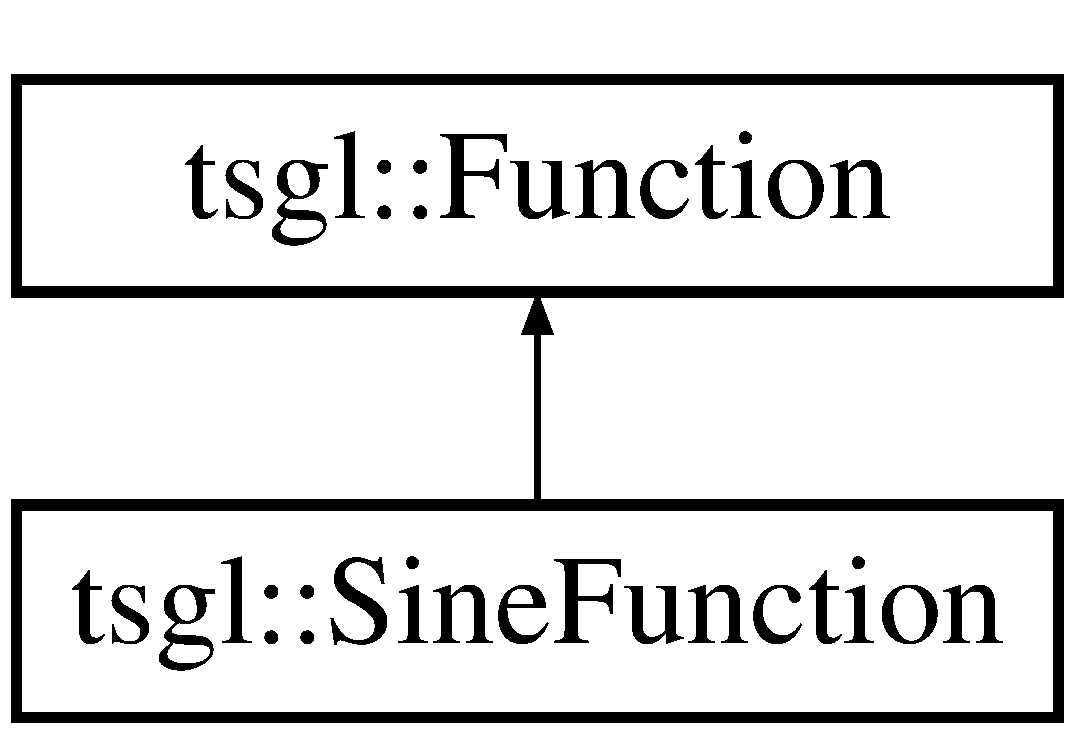
\includegraphics[height=2.000000cm]{classtsgl_1_1_sine_function}
\end{center}
\end{figure}
\subsection*{Public Member Functions}
\begin{DoxyCompactItemize}
\item 
virtual Decimal \hyperlink{classtsgl_1_1_sine_function_a4a34d3310ea217255124d5e35805be3a}{value\+At} (Decimal x) const
\begin{DoxyCompactList}\small\item\em Method to determine the value of \hyperlink{classtsgl_1_1_sine_function}{Sine\+Function}. \end{DoxyCompactList}\end{DoxyCompactItemize}


\subsection{Detailed Description}
\hyperlink{classtsgl_1_1_function}{Function} to compute the sine of the input. 

\subsection{Member Function Documentation}
\mbox{\Hypertarget{classtsgl_1_1_sine_function_a4a34d3310ea217255124d5e35805be3a}\label{classtsgl_1_1_sine_function_a4a34d3310ea217255124d5e35805be3a}} 
\index{tsgl\+::\+Sine\+Function@{tsgl\+::\+Sine\+Function}!value\+At@{value\+At}}
\index{value\+At@{value\+At}!tsgl\+::\+Sine\+Function@{tsgl\+::\+Sine\+Function}}
\subsubsection{\texorpdfstring{value\+At()}{valueAt()}}
{\footnotesize\ttfamily virtual Decimal tsgl\+::\+Sine\+Function\+::value\+At (\begin{DoxyParamCaption}\item[{Decimal}]{x }\end{DoxyParamCaption}) const\hspace{0.3cm}{\ttfamily [inline]}, {\ttfamily [virtual]}}



Method to determine the value of \hyperlink{classtsgl_1_1_sine_function}{Sine\+Function}. 

\begin{DoxyReturn}{Returns}
The sine of {\itshape x}. 
\end{DoxyReturn}


Implements \hyperlink{classtsgl_1_1_function_affb7b3b19a04efefa29a9870d666e912}{tsgl\+::\+Function}.



The documentation for this class was generated from the following file\+:\begin{DoxyCompactItemize}
\item 
Function.\+h\end{DoxyCompactItemize}

\hypertarget{classtsgl_1_1_spectrogram}{}\section{tsgl\+:\+:Spectrogram Class Reference}
\label{classtsgl_1_1_spectrogram}\index{tsgl\+::\+Spectrogram@{tsgl\+::\+Spectrogram}}


Displays a spectrogram of a given data set.  




{\ttfamily \#include $<$Spectrogram.\+h$>$}

\subsection*{Public Member Functions}
\begin{DoxyCompactItemize}
\item 
\hyperlink{classtsgl_1_1_spectrogram_a806d3244b086b9ed2c982b7178eb5139}{Spectrogram} (Spectrogram\+Drawmode draw\+Mode, int width, int height=-\/1)
\begin{DoxyCompactList}\small\item\em Explicit \hyperlink{classtsgl_1_1_spectrogram}{Spectrogram} constructor method. \end{DoxyCompactList}\item 
\hyperlink{classtsgl_1_1_spectrogram_abf1ff8d5acade39017321d6a2006f0f1}{$\sim$\+Spectrogram} ()
\begin{DoxyCompactList}\small\item\em \hyperlink{classtsgl_1_1_spectrogram}{Spectrogram} destructor method. \end{DoxyCompactList}\item 
void \hyperlink{classtsgl_1_1_spectrogram_a8fc0e145d5ad8673cc51876e698fb162}{update} (int index, float weight=1.\+0f, float decay=0.\+8f)
\begin{DoxyCompactList}\small\item\em Updates a spectrogram with new data. \end{DoxyCompactList}\item 
void \hyperlink{classtsgl_1_1_spectrogram_aef15257f0daa13a57d99cd621d402bd5}{draw} (float ratio)
\begin{DoxyCompactList}\small\item\em Updates the image on the spectrogram. \end{DoxyCompactList}\item 
void \hyperlink{classtsgl_1_1_spectrogram_a9e6eb0489ee0fb9f96b2a5202868a1c2}{finish} ()
\begin{DoxyCompactList}\small\item\em Finishes the spectrogram. \end{DoxyCompactList}\end{DoxyCompactItemize}


\subsection{Detailed Description}
Displays a spectrogram of a given data set. 

\hyperlink{classtsgl_1_1_spectrogram}{Spectrogram} is a class for visualizing data as a color spectrum. This data will typically be hues, but \hyperlink{classtsgl_1_1_spectrogram}{Spectrogram} will accept any data mapping to an integer value between 0 and 255. 

\subsection{Constructor \& Destructor Documentation}
\hypertarget{classtsgl_1_1_spectrogram_a806d3244b086b9ed2c982b7178eb5139}{}\index{tsgl\+::\+Spectrogram@{tsgl\+::\+Spectrogram}!Spectrogram@{Spectrogram}}
\index{Spectrogram@{Spectrogram}!tsgl\+::\+Spectrogram@{tsgl\+::\+Spectrogram}}
\subsubsection[{Spectrogram}]{\setlength{\rightskip}{0pt plus 5cm}tsgl\+::\+Spectrogram\+::\+Spectrogram (
\begin{DoxyParamCaption}
\item[{Spectrogram\+Drawmode}]{draw\+Mode, }
\item[{int}]{width, }
\item[{int}]{height = {\ttfamily -\/1}}
\end{DoxyParamCaption}
)}\label{classtsgl_1_1_spectrogram_a806d3244b086b9ed2c982b7178eb5139}


Explicit \hyperlink{classtsgl_1_1_spectrogram}{Spectrogram} constructor method. 

This is the explicit constructor for the \hyperlink{classtsgl_1_1_spectrogram}{Spectrogram} class. 
\begin{DoxyParams}{Parameters}
{\em draw\+Mode} & Method used for displaying spectral data. Can be one of C\+I\+R\+C\+U\+L\+A\+R or H\+O\+R\+I\+Z\+O\+N\+T\+A\+L. \\
\hline
{\em width} & The width of the \hyperlink{classtsgl_1_1_spectrogram}{Spectrogram} canvas. \\
\hline
{\em height} & The height of the \hyperlink{classtsgl_1_1_spectrogram}{Spectrogram} canvas. This value is ignored for H\+O\+R\+I\+Z\+O\+N\+T\+A\+L Spectrograms. Setting this to -\/1 sets the width automatically. \\
\hline
\end{DoxyParams}
\begin{DoxyReturn}{Returns}
A new \hyperlink{classtsgl_1_1_spectrogram}{Spectrogram} with the specified drawing mode and size. 
\end{DoxyReturn}
\hypertarget{classtsgl_1_1_spectrogram_abf1ff8d5acade39017321d6a2006f0f1}{}\index{tsgl\+::\+Spectrogram@{tsgl\+::\+Spectrogram}!````~Spectrogram@{$\sim$\+Spectrogram}}
\index{````~Spectrogram@{$\sim$\+Spectrogram}!tsgl\+::\+Spectrogram@{tsgl\+::\+Spectrogram}}
\subsubsection[{$\sim$\+Spectrogram}]{\setlength{\rightskip}{0pt plus 5cm}tsgl\+::\+Spectrogram\+::$\sim$\+Spectrogram (
\begin{DoxyParamCaption}
{}
\end{DoxyParamCaption}
)}\label{classtsgl_1_1_spectrogram_abf1ff8d5acade39017321d6a2006f0f1}


\hyperlink{classtsgl_1_1_spectrogram}{Spectrogram} destructor method. 

This is the destructor for the \hyperlink{classtsgl_1_1_spectrogram}{Spectrogram} class.

Frees up memory that was allocated to a \hyperlink{classtsgl_1_1_spectrogram}{Spectrogram} instance. 

\subsection{Member Function Documentation}
\hypertarget{classtsgl_1_1_spectrogram_aef15257f0daa13a57d99cd621d402bd5}{}\index{tsgl\+::\+Spectrogram@{tsgl\+::\+Spectrogram}!draw@{draw}}
\index{draw@{draw}!tsgl\+::\+Spectrogram@{tsgl\+::\+Spectrogram}}
\subsubsection[{draw}]{\setlength{\rightskip}{0pt plus 5cm}void tsgl\+::\+Spectrogram\+::draw (
\begin{DoxyParamCaption}
\item[{float}]{ratio}
\end{DoxyParamCaption}
)}\label{classtsgl_1_1_spectrogram_aef15257f0daa13a57d99cd621d402bd5}


Updates the image on the spectrogram. 

This function updates the \hyperlink{classtsgl_1_1_spectrogram}{Spectrogram}\textquotesingle{}s \hyperlink{classtsgl_1_1_canvas}{Canvas} with the data since the last call to \hyperlink{classtsgl_1_1_spectrogram_a8fc0e145d5ad8673cc51876e698fb162}{update()} and redraws it. 
\begin{DoxyParams}{Parameters}
{\em ratio} & The scaling of the visualizer. Accepts values between 0.\+0f and 1.\+0f. \\
\hline
\end{DoxyParams}
\hypertarget{classtsgl_1_1_spectrogram_a9e6eb0489ee0fb9f96b2a5202868a1c2}{}\index{tsgl\+::\+Spectrogram@{tsgl\+::\+Spectrogram}!finish@{finish}}
\index{finish@{finish}!tsgl\+::\+Spectrogram@{tsgl\+::\+Spectrogram}}
\subsubsection[{finish}]{\setlength{\rightskip}{0pt plus 5cm}void tsgl\+::\+Spectrogram\+::finish (
\begin{DoxyParamCaption}
{}
\end{DoxyParamCaption}
)}\label{classtsgl_1_1_spectrogram_a9e6eb0489ee0fb9f96b2a5202868a1c2}


Finishes the spectrogram. 

This function tells the \hyperlink{classtsgl_1_1_spectrogram}{Spectrogram} to free all of its memory and close down its \hyperlink{classtsgl_1_1_canvas}{Canvas}. \hypertarget{classtsgl_1_1_spectrogram_a8fc0e145d5ad8673cc51876e698fb162}{}\index{tsgl\+::\+Spectrogram@{tsgl\+::\+Spectrogram}!update@{update}}
\index{update@{update}!tsgl\+::\+Spectrogram@{tsgl\+::\+Spectrogram}}
\subsubsection[{update}]{\setlength{\rightskip}{0pt plus 5cm}void tsgl\+::\+Spectrogram\+::update (
\begin{DoxyParamCaption}
\item[{int}]{index, }
\item[{float}]{weight = {\ttfamily 1.0f}, }
\item[{float}]{decay = {\ttfamily 0.8f}}
\end{DoxyParamCaption}
)}\label{classtsgl_1_1_spectrogram_a8fc0e145d5ad8673cc51876e698fb162}


Updates a spectrogram with new data. 

This function adds the value of {\ttfamily weight} to the hue specified by {\ttfamily index}, and adds the value ({\ttfamily decay}$^\wedge${\ttfamily n})$\ast$ {\ttfamily weight} to all hues {\ttfamily n} steps away from {\ttfamily index}. 
\begin{DoxyParams}{Parameters}
{\em index} & Index of the hue to update. Value is taken mod 256. \\
\hline
{\em weight} & The value to add to {\ttfamily index}. \\
\hline
{\em decay} & Falloff for {\ttfamily weight} upon adjacent values. \\
\hline
\end{DoxyParams}


The documentation for this class was generated from the following files\+:\begin{DoxyCompactItemize}
\item 
Spectrogram.\+h\item 
Spectrogram.\+cpp\end{DoxyCompactItemize}

\hypertarget{classtsgl_1_1_sphere}{}\section{tsgl\+:\+:Sphere Class Reference}
\label{classtsgl_1_1_sphere}\index{tsgl\+::\+Sphere@{tsgl\+::\+Sphere}}


Draw an arbitrary \hyperlink{classtsgl_1_1_sphere}{Sphere} with colored vertices.  




{\ttfamily \#include $<$Sphere.\+h$>$}

Inheritance diagram for tsgl\+:\+:Sphere\+:\begin{figure}[H]
\begin{center}
\leavevmode
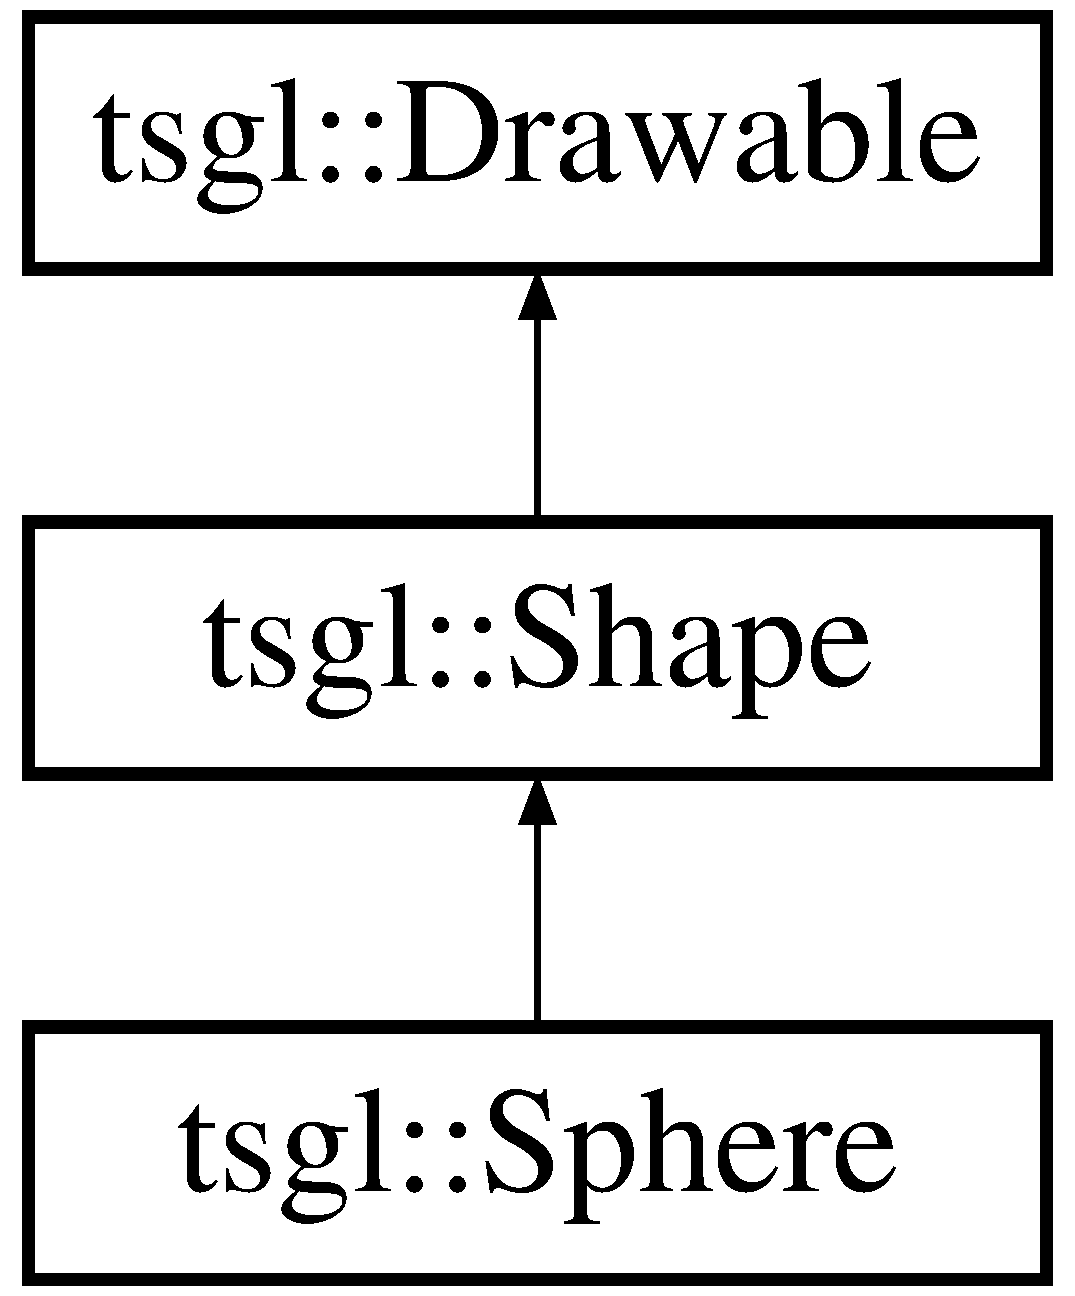
\includegraphics[height=3.000000cm]{classtsgl_1_1_sphere}
\end{center}
\end{figure}
\subsection*{Public Member Functions}
\begin{DoxyCompactItemize}
\item 
\hyperlink{classtsgl_1_1_sphere_a80d326f71e37a88274d479c87ad96efe}{Sphere} (float x, float y, float z, G\+Lfloat radius, float yaw, float pitch, float roll, \hyperlink{structtsgl_1_1_color_float}{Color\+Float} c)
\begin{DoxyCompactList}\small\item\em Explicitly constructs a new \hyperlink{classtsgl_1_1_sphere}{Sphere}. \end{DoxyCompactList}\item 
\hyperlink{classtsgl_1_1_sphere_adcf41c60e73de7447b9720272c0200aa}{Sphere} (float x, float y, float z, G\+Lfloat radius, float yaw, float pitch, float roll, \hyperlink{structtsgl_1_1_color_float}{Color\+Float} c\mbox{[}$\,$\mbox{]})
\begin{DoxyCompactList}\small\item\em Explicitly constructs a new \hyperlink{classtsgl_1_1_sphere}{Sphere}. \end{DoxyCompactList}\item 
virtual void \hyperlink{classtsgl_1_1_sphere_a7d1f92b4c10a165b909cb6edb12288d5}{set\+Radius} (float radius)
\begin{DoxyCompactList}\small\item\em Mutates the \hyperlink{classtsgl_1_1_sphere}{Sphere}\textquotesingle{}s radius. \end{DoxyCompactList}\item 
virtual void \hyperlink{classtsgl_1_1_sphere_afeddb373be43550a1e3386d53332dd6f}{change\+Radius\+By} (float delta)
\begin{DoxyCompactList}\small\item\em Mutates the \hyperlink{classtsgl_1_1_sphere}{Sphere}\textquotesingle{}s radius by the parameter amount. \end{DoxyCompactList}\item 
\mbox{\Hypertarget{classtsgl_1_1_sphere_a465494e673964c2fde85ed9b342a665d}\label{classtsgl_1_1_sphere_a465494e673964c2fde85ed9b342a665d}} 
virtual G\+Lfloat {\bfseries get\+Radius} ()
\item 
virtual void \hyperlink{classtsgl_1_1_sphere_aa0870a70e34c6c77e2d61e50dbf3cc07}{set\+Color} (\hyperlink{structtsgl_1_1_color_float}{Color\+Float} c)
\begin{DoxyCompactList}\small\item\em Sets the \hyperlink{classtsgl_1_1_sphere}{Sphere} to a new color. \end{DoxyCompactList}\item 
virtual void \hyperlink{classtsgl_1_1_sphere_aab902ab87c24e7065c74f553f7e8c126}{set\+Color} (\hyperlink{structtsgl_1_1_color_float}{Color\+Float} c\mbox{[}$\,$\mbox{]})
\begin{DoxyCompactList}\small\item\em Sets the \hyperlink{classtsgl_1_1_sphere}{Sphere} to an array of new colors. \end{DoxyCompactList}\item 
virtual void \hyperlink{classtsgl_1_1_sphere_a767bfb1b0c6c29d0577377aa0403d881}{get\+Colors} (std\+::vector$<$ \hyperlink{structtsgl_1_1_color_float}{Color\+Float} $>$ \&color\+Vec)
\begin{DoxyCompactList}\small\item\em Accessor for \hyperlink{classtsgl_1_1_sphere}{Sphere}\textquotesingle{}s colors. \end{DoxyCompactList}\end{DoxyCompactItemize}
\subsection*{Protected Attributes}
\begin{DoxyCompactItemize}
\item 
\mbox{\Hypertarget{classtsgl_1_1_sphere_ab4d6cee5f4c8ce474b58f3d528d5ef64}\label{classtsgl_1_1_sphere_ab4d6cee5f4c8ce474b58f3d528d5ef64}} 
G\+Lfloat {\bfseries my\+Radius}
\item 
\mbox{\Hypertarget{classtsgl_1_1_sphere_a00159df8b6b14b13423a5654312bd0b6}\label{classtsgl_1_1_sphere_a00159df8b6b14b13423a5654312bd0b6}} 
int {\bfseries horizontal\+Sections}
\item 
\mbox{\Hypertarget{classtsgl_1_1_sphere_abed42db5d3fa69211ba25fb03ba6d23f}\label{classtsgl_1_1_sphere_abed42db5d3fa69211ba25fb03ba6d23f}} 
int {\bfseries vertical\+Sections}
\end{DoxyCompactItemize}
\subsection*{Additional Inherited Members}


\subsection{Detailed Description}
Draw an arbitrary \hyperlink{classtsgl_1_1_sphere}{Sphere} with colored vertices. 

\hyperlink{classtsgl_1_1_sphere}{Sphere} is a class for holding vertex data for a \hyperlink{classtsgl_1_1_sphere}{Sphere} with non-\/negative radius. 

\subsection{Constructor \& Destructor Documentation}
\mbox{\Hypertarget{classtsgl_1_1_sphere_a80d326f71e37a88274d479c87ad96efe}\label{classtsgl_1_1_sphere_a80d326f71e37a88274d479c87ad96efe}} 
\index{tsgl\+::\+Sphere@{tsgl\+::\+Sphere}!Sphere@{Sphere}}
\index{Sphere@{Sphere}!tsgl\+::\+Sphere@{tsgl\+::\+Sphere}}
\subsubsection{\texorpdfstring{Sphere()}{Sphere()}\hspace{0.1cm}{\footnotesize\ttfamily [1/2]}}
{\footnotesize\ttfamily tsgl\+::\+Sphere\+::\+Sphere (\begin{DoxyParamCaption}\item[{float}]{x,  }\item[{float}]{y,  }\item[{float}]{z,  }\item[{G\+Lfloat}]{radius,  }\item[{float}]{yaw,  }\item[{float}]{pitch,  }\item[{float}]{roll,  }\item[{\hyperlink{structtsgl_1_1_color_float}{Color\+Float}}]{c }\end{DoxyParamCaption})}



Explicitly constructs a new \hyperlink{classtsgl_1_1_sphere}{Sphere}. 

Explicit constructor for a \hyperlink{classtsgl_1_1_sphere}{Sphere} object. 
\begin{DoxyParams}{Parameters}
{\em x} & The x coordinate of the center of the \hyperlink{classtsgl_1_1_sphere}{Sphere}. \\
\hline
{\em y} & The y coordinate of the center of the \hyperlink{classtsgl_1_1_sphere}{Sphere}. \\
\hline
{\em z} & The z coordinate of the center of the \hyperlink{classtsgl_1_1_sphere}{Sphere}. \\
\hline
{\em radius} & The \hyperlink{classtsgl_1_1_sphere}{Sphere}\textquotesingle{}s radius \\
\hline
{\em yaw} & The \hyperlink{classtsgl_1_1_sphere}{Sphere}\textquotesingle{}s yaw. \\
\hline
{\em pitch} & The \hyperlink{classtsgl_1_1_sphere}{Sphere}\textquotesingle{}s pitch. \\
\hline
{\em roll} & The \hyperlink{classtsgl_1_1_sphere}{Sphere}\textquotesingle{}s roll. \\
\hline
{\em c} & A \hyperlink{structtsgl_1_1_color_float}{Color\+Float} for the \hyperlink{classtsgl_1_1_sphere}{Sphere}\textquotesingle{}s vertex colors. \\
\hline
\end{DoxyParams}
\begin{DoxyWarning}{Warning}
An invariant is held where if radius isn\textquotesingle{}t positive then an error message is given. 
\end{DoxyWarning}
\begin{DoxyReturn}{Returns}
A new \hyperlink{classtsgl_1_1_sphere}{Sphere} with a buffer for storing the specified numbered of vertices. 
\end{DoxyReturn}
\mbox{\Hypertarget{classtsgl_1_1_sphere_adcf41c60e73de7447b9720272c0200aa}\label{classtsgl_1_1_sphere_adcf41c60e73de7447b9720272c0200aa}} 
\index{tsgl\+::\+Sphere@{tsgl\+::\+Sphere}!Sphere@{Sphere}}
\index{Sphere@{Sphere}!tsgl\+::\+Sphere@{tsgl\+::\+Sphere}}
\subsubsection{\texorpdfstring{Sphere()}{Sphere()}\hspace{0.1cm}{\footnotesize\ttfamily [2/2]}}
{\footnotesize\ttfamily tsgl\+::\+Sphere\+::\+Sphere (\begin{DoxyParamCaption}\item[{float}]{x,  }\item[{float}]{y,  }\item[{float}]{z,  }\item[{G\+Lfloat}]{radius,  }\item[{float}]{yaw,  }\item[{float}]{pitch,  }\item[{float}]{roll,  }\item[{\hyperlink{structtsgl_1_1_color_float}{Color\+Float}}]{c\mbox{[}$\,$\mbox{]} }\end{DoxyParamCaption})}



Explicitly constructs a new \hyperlink{classtsgl_1_1_sphere}{Sphere}. 

Explicit constructor for a \hyperlink{classtsgl_1_1_sphere}{Sphere} object. 
\begin{DoxyParams}{Parameters}
{\em x} & The x coordinate of the center of the \hyperlink{classtsgl_1_1_sphere}{Sphere}. \\
\hline
{\em y} & The y coordinate of the center of the \hyperlink{classtsgl_1_1_sphere}{Sphere}. \\
\hline
{\em z} & The z coordinate of the center of the \hyperlink{classtsgl_1_1_sphere}{Sphere}. \\
\hline
{\em radius} & The distance from the center of the \hyperlink{classtsgl_1_1_sphere}{Sphere}\textquotesingle{}s base to each vertex of the base. \\
\hline
{\em yaw} & The \hyperlink{classtsgl_1_1_sphere}{Sphere}\textquotesingle{}s yaw. \\
\hline
{\em pitch} & The \hyperlink{classtsgl_1_1_sphere}{Sphere}\textquotesingle{}s pitch. \\
\hline
{\em roll} & The \hyperlink{classtsgl_1_1_sphere}{Sphere}\textquotesingle{}s roll. \\
\hline
{\em c} & An array of Color\+Floats for the \hyperlink{classtsgl_1_1_sphere}{Sphere}\textquotesingle{}s vertex colors. \\
\hline
\end{DoxyParams}
\begin{DoxyWarning}{Warning}
An invariant is held where if radius isn\textquotesingle{}t positive then an error message is given. 
\end{DoxyWarning}
\begin{DoxyReturn}{Returns}
A new \hyperlink{classtsgl_1_1_sphere}{Sphere} with a buffer for storing the specified numbered of vertices. 
\end{DoxyReturn}


\subsection{Member Function Documentation}
\mbox{\Hypertarget{classtsgl_1_1_sphere_afeddb373be43550a1e3386d53332dd6f}\label{classtsgl_1_1_sphere_afeddb373be43550a1e3386d53332dd6f}} 
\index{tsgl\+::\+Sphere@{tsgl\+::\+Sphere}!change\+Radius\+By@{change\+Radius\+By}}
\index{change\+Radius\+By@{change\+Radius\+By}!tsgl\+::\+Sphere@{tsgl\+::\+Sphere}}
\subsubsection{\texorpdfstring{change\+Radius\+By()}{changeRadiusBy()}}
{\footnotesize\ttfamily void tsgl\+::\+Sphere\+::change\+Radius\+By (\begin{DoxyParamCaption}\item[{float}]{delta }\end{DoxyParamCaption})\hspace{0.3cm}{\ttfamily [virtual]}}



Mutates the \hyperlink{classtsgl_1_1_sphere}{Sphere}\textquotesingle{}s radius by the parameter amount. 


\begin{DoxyParams}{Parameters}
{\em delta} & The amount by which to change the radius of the \hyperlink{classtsgl_1_1_sphere}{Sphere}. \\
\hline
\end{DoxyParams}
\mbox{\Hypertarget{classtsgl_1_1_sphere_a767bfb1b0c6c29d0577377aa0403d881}\label{classtsgl_1_1_sphere_a767bfb1b0c6c29d0577377aa0403d881}} 
\index{tsgl\+::\+Sphere@{tsgl\+::\+Sphere}!get\+Colors@{get\+Colors}}
\index{get\+Colors@{get\+Colors}!tsgl\+::\+Sphere@{tsgl\+::\+Sphere}}
\subsubsection{\texorpdfstring{get\+Colors()}{getColors()}}
{\footnotesize\ttfamily void tsgl\+::\+Sphere\+::get\+Colors (\begin{DoxyParamCaption}\item[{std\+::vector$<$ \hyperlink{structtsgl_1_1_color_float}{Color\+Float} $>$ \&}]{color\+Vec }\end{DoxyParamCaption})\hspace{0.3cm}{\ttfamily [virtual]}}



Accessor for \hyperlink{classtsgl_1_1_sphere}{Sphere}\textquotesingle{}s colors. 

Populates the reference parameter vector with a \hyperlink{structtsgl_1_1_color_float}{Color\+Float} for each vertical section of \hyperlink{classtsgl_1_1_sphere}{Sphere}. 
\begin{DoxyParams}{Parameters}
{\em color\+Vec} & A vector of Color\+Floats to which the Color\+Floats associated with \hyperlink{classtsgl_1_1_sphere}{Sphere} will be pushed. \\
\hline
\end{DoxyParams}
\begin{DoxyNote}{Note}
Overrides \hyperlink{classtsgl_1_1_shape_a6f54fe4d049f69a287edf8335a9509f8}{Shape\+::get\+Colors()}. 
\end{DoxyNote}


Reimplemented from \hyperlink{classtsgl_1_1_shape_a6f54fe4d049f69a287edf8335a9509f8}{tsgl\+::\+Shape}.

\mbox{\Hypertarget{classtsgl_1_1_sphere_aa0870a70e34c6c77e2d61e50dbf3cc07}\label{classtsgl_1_1_sphere_aa0870a70e34c6c77e2d61e50dbf3cc07}} 
\index{tsgl\+::\+Sphere@{tsgl\+::\+Sphere}!set\+Color@{set\+Color}}
\index{set\+Color@{set\+Color}!tsgl\+::\+Sphere@{tsgl\+::\+Sphere}}
\subsubsection{\texorpdfstring{set\+Color()}{setColor()}\hspace{0.1cm}{\footnotesize\ttfamily [1/2]}}
{\footnotesize\ttfamily void tsgl\+::\+Sphere\+::set\+Color (\begin{DoxyParamCaption}\item[{\hyperlink{structtsgl_1_1_color_float}{Color\+Float}}]{c }\end{DoxyParamCaption})\hspace{0.3cm}{\ttfamily [virtual]}}



Sets the \hyperlink{classtsgl_1_1_sphere}{Sphere} to a new color. 


\begin{DoxyParams}{Parameters}
{\em c} & The new \hyperlink{structtsgl_1_1_color_float}{Color\+Float}. \\
\hline
\end{DoxyParams}


Reimplemented from \hyperlink{classtsgl_1_1_shape_abdb01321cddfd2db1481eefbc2836f70}{tsgl\+::\+Shape}.

\mbox{\Hypertarget{classtsgl_1_1_sphere_aab902ab87c24e7065c74f553f7e8c126}\label{classtsgl_1_1_sphere_aab902ab87c24e7065c74f553f7e8c126}} 
\index{tsgl\+::\+Sphere@{tsgl\+::\+Sphere}!set\+Color@{set\+Color}}
\index{set\+Color@{set\+Color}!tsgl\+::\+Sphere@{tsgl\+::\+Sphere}}
\subsubsection{\texorpdfstring{set\+Color()}{setColor()}\hspace{0.1cm}{\footnotesize\ttfamily [2/2]}}
{\footnotesize\ttfamily void tsgl\+::\+Sphere\+::set\+Color (\begin{DoxyParamCaption}\item[{\hyperlink{structtsgl_1_1_color_float}{Color\+Float}}]{c\mbox{[}$\,$\mbox{]} }\end{DoxyParamCaption})\hspace{0.3cm}{\ttfamily [virtual]}}



Sets the \hyperlink{classtsgl_1_1_sphere}{Sphere} to an array of new colors. 


\begin{DoxyParams}{Parameters}
{\em c} & An array of new Color\+Floats.\\
\hline
\end{DoxyParams}
The array should have 20 \hyperlink{structtsgl_1_1_color_float}{Color\+Float} minimum, one for each horizontal section. 

Reimplemented from \hyperlink{classtsgl_1_1_shape_ad7e554b5d4cea111ec518548b9f21388}{tsgl\+::\+Shape}.

\mbox{\Hypertarget{classtsgl_1_1_sphere_a7d1f92b4c10a165b909cb6edb12288d5}\label{classtsgl_1_1_sphere_a7d1f92b4c10a165b909cb6edb12288d5}} 
\index{tsgl\+::\+Sphere@{tsgl\+::\+Sphere}!set\+Radius@{set\+Radius}}
\index{set\+Radius@{set\+Radius}!tsgl\+::\+Sphere@{tsgl\+::\+Sphere}}
\subsubsection{\texorpdfstring{set\+Radius()}{setRadius()}}
{\footnotesize\ttfamily void tsgl\+::\+Sphere\+::set\+Radius (\begin{DoxyParamCaption}\item[{float}]{radius }\end{DoxyParamCaption})\hspace{0.3cm}{\ttfamily [virtual]}}



Mutates the \hyperlink{classtsgl_1_1_sphere}{Sphere}\textquotesingle{}s radius. 


\begin{DoxyParams}{Parameters}
{\em radius} & The new radius of the \hyperlink{classtsgl_1_1_sphere}{Sphere}. \\
\hline
\end{DoxyParams}


The documentation for this class was generated from the following files\+:\begin{DoxyCompactItemize}
\item 
Sphere.\+h\item 
Sphere.\+cpp\end{DoxyCompactItemize}

\hypertarget{classtsgl_1_1_square}{}\section{tsgl\+:\+:Square Class Reference}
\label{classtsgl_1_1_square}\index{tsgl\+::\+Square@{tsgl\+::\+Square}}


Draw a square.  




{\ttfamily \#include $<$Square.\+h$>$}

Inheritance diagram for tsgl\+:\+:Square\+:\begin{figure}[H]
\begin{center}
\leavevmode
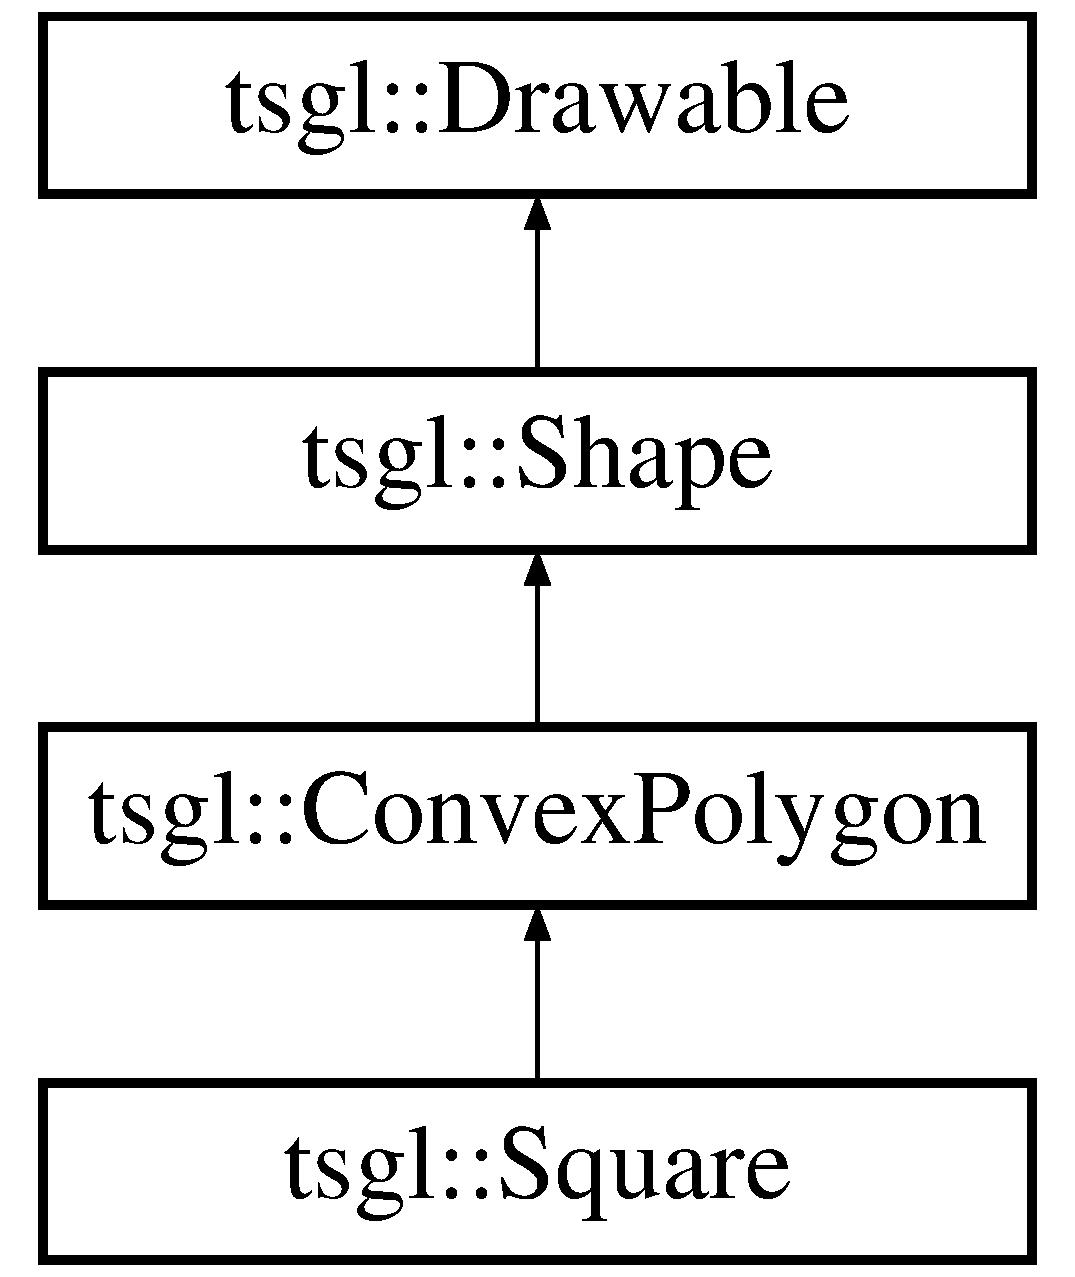
\includegraphics[height=4.000000cm]{classtsgl_1_1_square}
\end{center}
\end{figure}
\subsection*{Public Member Functions}
\begin{DoxyCompactItemize}
\item 
\hyperlink{classtsgl_1_1_square_a1279be7f6ddfc10491c6d77ff9cc18bf}{Square} (float x, float y, float z, G\+Lfloat side\+Length, float yaw, float pitch, float roll, \hyperlink{structtsgl_1_1_color_float}{Color\+Float} color)
\begin{DoxyCompactList}\small\item\em Explicitly constructs a new \hyperlink{classtsgl_1_1_square}{Square} with monocolored fill. \end{DoxyCompactList}\item 
\hyperlink{classtsgl_1_1_square_a9c8c6685801135adbb3ca4c94c0df4a3}{Square} (float x, float y, float z, G\+Lfloat side\+Length, float yaw, float pitch, float roll, \hyperlink{structtsgl_1_1_color_float}{Color\+Float} color\mbox{[}$\,$\mbox{]})
\begin{DoxyCompactList}\small\item\em Explicitly constructs a new \hyperlink{classtsgl_1_1_square}{Square} with multicolored fill. \end{DoxyCompactList}\item 
G\+Lfloat \hyperlink{classtsgl_1_1_square_adf0871e17342a6a44361463015c5bc46}{get\+Side\+Length} ()
\begin{DoxyCompactList}\small\item\em Accessor for the side length of the \hyperlink{classtsgl_1_1_square}{Square}. \end{DoxyCompactList}\item 
void \hyperlink{classtsgl_1_1_square_a0517236849893cdf0ab097df69e3416d}{set\+Side\+Length} (G\+Lfloat side\+Length)
\begin{DoxyCompactList}\small\item\em Mutates the distance between opposite sides of the \hyperlink{classtsgl_1_1_square}{Square}. \end{DoxyCompactList}\item 
void \hyperlink{classtsgl_1_1_square_a9804eb52021958970ff482625682d0d0}{change\+Side\+Length\+By} (G\+Lfloat delta)
\begin{DoxyCompactList}\small\item\em Mutates the distance between opposite sides of the \hyperlink{classtsgl_1_1_square}{Square} by the parameter amount. \end{DoxyCompactList}\end{DoxyCompactItemize}
\subsection*{Protected Attributes}
\begin{DoxyCompactItemize}
\item 
\mbox{\Hypertarget{classtsgl_1_1_square_a501911f1f20111d504f756b437bccdaf}\label{classtsgl_1_1_square_a501911f1f20111d504f756b437bccdaf}} 
G\+Lfloat {\bfseries my\+Side\+Length}
\end{DoxyCompactItemize}
\subsection*{Additional Inherited Members}


\subsection{Detailed Description}
Draw a square. 

\hyperlink{classtsgl_1_1_square}{Square} is a class for holding \hyperlink{classtsgl_1_1_shape}{Shape} data for a square. 

\subsection{Constructor \& Destructor Documentation}
\mbox{\Hypertarget{classtsgl_1_1_square_a1279be7f6ddfc10491c6d77ff9cc18bf}\label{classtsgl_1_1_square_a1279be7f6ddfc10491c6d77ff9cc18bf}} 
\index{tsgl\+::\+Square@{tsgl\+::\+Square}!Square@{Square}}
\index{Square@{Square}!tsgl\+::\+Square@{tsgl\+::\+Square}}
\subsubsection{\texorpdfstring{Square()}{Square()}\hspace{0.1cm}{\footnotesize\ttfamily [1/2]}}
{\footnotesize\ttfamily tsgl\+::\+Square\+::\+Square (\begin{DoxyParamCaption}\item[{float}]{x,  }\item[{float}]{y,  }\item[{float}]{z,  }\item[{G\+Lfloat}]{side\+Length,  }\item[{float}]{yaw,  }\item[{float}]{pitch,  }\item[{float}]{roll,  }\item[{\hyperlink{structtsgl_1_1_color_float}{Color\+Float}}]{color }\end{DoxyParamCaption})}



Explicitly constructs a new \hyperlink{classtsgl_1_1_square}{Square} with monocolored fill. 

This function draws a \hyperlink{classtsgl_1_1_square}{Square} with the given center, sidelength, rotation, and color. 
\begin{DoxyParams}{Parameters}
{\em x} & The x coordinate of the \hyperlink{classtsgl_1_1_square}{Square}\textquotesingle{}s center. \\
\hline
{\em y} & The y coordinate of the \hyperlink{classtsgl_1_1_square}{Square}\textquotesingle{}s center. \\
\hline
{\em z} & The z coordinate of the \hyperlink{classtsgl_1_1_square}{Square}\textquotesingle{}s center. \\
\hline
{\em side\+Length} & The side length of the \hyperlink{classtsgl_1_1_square}{Square} in pixels. \\
\hline
{\em yaw} & The \hyperlink{classtsgl_1_1_square}{Square}\textquotesingle{}s yaw in 3D space. \\
\hline
{\em pitch} & The \hyperlink{classtsgl_1_1_square}{Square}\textquotesingle{}s pitch in 3D space. \\
\hline
{\em roll} & The \hyperlink{classtsgl_1_1_square}{Square}\textquotesingle{}s roll in 3D space. \\
\hline
{\em color} & The color of the \hyperlink{classtsgl_1_1_square}{Square}. \\
\hline
\end{DoxyParams}
\mbox{\Hypertarget{classtsgl_1_1_square_a9c8c6685801135adbb3ca4c94c0df4a3}\label{classtsgl_1_1_square_a9c8c6685801135adbb3ca4c94c0df4a3}} 
\index{tsgl\+::\+Square@{tsgl\+::\+Square}!Square@{Square}}
\index{Square@{Square}!tsgl\+::\+Square@{tsgl\+::\+Square}}
\subsubsection{\texorpdfstring{Square()}{Square()}\hspace{0.1cm}{\footnotesize\ttfamily [2/2]}}
{\footnotesize\ttfamily tsgl\+::\+Square\+::\+Square (\begin{DoxyParamCaption}\item[{float}]{x,  }\item[{float}]{y,  }\item[{float}]{z,  }\item[{G\+Lfloat}]{side\+Length,  }\item[{float}]{yaw,  }\item[{float}]{pitch,  }\item[{float}]{roll,  }\item[{\hyperlink{structtsgl_1_1_color_float}{Color\+Float}}]{color\mbox{[}$\,$\mbox{]} }\end{DoxyParamCaption})}



Explicitly constructs a new \hyperlink{classtsgl_1_1_square}{Square} with multicolored fill. 

This function draws a \hyperlink{classtsgl_1_1_square}{Square} with the given center, sidelength, rotation, and color. 
\begin{DoxyParams}{Parameters}
{\em x} & The x coordinate of the \hyperlink{classtsgl_1_1_square}{Square}\textquotesingle{}s center. \\
\hline
{\em y} & The y coordinate of the \hyperlink{classtsgl_1_1_square}{Square}\textquotesingle{}s center. \\
\hline
{\em z} & The z coordinate of the \hyperlink{classtsgl_1_1_square}{Square}\textquotesingle{}s center. \\
\hline
{\em side\+Length} & The side length of the \hyperlink{classtsgl_1_1_square}{Square} in pixels. \\
\hline
{\em yaw} & The \hyperlink{classtsgl_1_1_square}{Square}\textquotesingle{}s yaw in 3D space. \\
\hline
{\em pitch} & The \hyperlink{classtsgl_1_1_square}{Square}\textquotesingle{}s pitch in 3D space. \\
\hline
{\em roll} & The \hyperlink{classtsgl_1_1_square}{Square}\textquotesingle{}s roll in 3D space. \\
\hline
{\em color} & An array of colors for the \hyperlink{classtsgl_1_1_square}{Square}\textquotesingle{}s vertices. \\
\hline
\end{DoxyParams}


\subsection{Member Function Documentation}
\mbox{\Hypertarget{classtsgl_1_1_square_a9804eb52021958970ff482625682d0d0}\label{classtsgl_1_1_square_a9804eb52021958970ff482625682d0d0}} 
\index{tsgl\+::\+Square@{tsgl\+::\+Square}!change\+Side\+Length\+By@{change\+Side\+Length\+By}}
\index{change\+Side\+Length\+By@{change\+Side\+Length\+By}!tsgl\+::\+Square@{tsgl\+::\+Square}}
\subsubsection{\texorpdfstring{change\+Side\+Length\+By()}{changeSideLengthBy()}}
{\footnotesize\ttfamily void tsgl\+::\+Square\+::change\+Side\+Length\+By (\begin{DoxyParamCaption}\item[{G\+Lfloat}]{delta }\end{DoxyParamCaption})}



Mutates the distance between opposite sides of the \hyperlink{classtsgl_1_1_square}{Square} by the parameter amount. 


\begin{DoxyParams}{Parameters}
{\em delta} & The amount by which to change the side length of the \hyperlink{classtsgl_1_1_square}{Square}. \\
\hline
\end{DoxyParams}


Referenced by get\+Side\+Length().

\mbox{\Hypertarget{classtsgl_1_1_square_adf0871e17342a6a44361463015c5bc46}\label{classtsgl_1_1_square_adf0871e17342a6a44361463015c5bc46}} 
\index{tsgl\+::\+Square@{tsgl\+::\+Square}!get\+Side\+Length@{get\+Side\+Length}}
\index{get\+Side\+Length@{get\+Side\+Length}!tsgl\+::\+Square@{tsgl\+::\+Square}}
\subsubsection{\texorpdfstring{get\+Side\+Length()}{getSideLength()}}
{\footnotesize\ttfamily G\+Lfloat tsgl\+::\+Square\+::get\+Side\+Length (\begin{DoxyParamCaption}{ }\end{DoxyParamCaption})\hspace{0.3cm}{\ttfamily [inline]}}



Accessor for the side length of the \hyperlink{classtsgl_1_1_square}{Square}. 

Returns the value of the my\+Side\+Length private variable, a G\+Lfloat. \mbox{\Hypertarget{classtsgl_1_1_square_a0517236849893cdf0ab097df69e3416d}\label{classtsgl_1_1_square_a0517236849893cdf0ab097df69e3416d}} 
\index{tsgl\+::\+Square@{tsgl\+::\+Square}!set\+Side\+Length@{set\+Side\+Length}}
\index{set\+Side\+Length@{set\+Side\+Length}!tsgl\+::\+Square@{tsgl\+::\+Square}}
\subsubsection{\texorpdfstring{set\+Side\+Length()}{setSideLength()}}
{\footnotesize\ttfamily void tsgl\+::\+Square\+::set\+Side\+Length (\begin{DoxyParamCaption}\item[{G\+Lfloat}]{side\+Length }\end{DoxyParamCaption})}



Mutates the distance between opposite sides of the \hyperlink{classtsgl_1_1_square}{Square}. 


\begin{DoxyParams}{Parameters}
{\em side\+Length} & The \hyperlink{classtsgl_1_1_square}{Square}\textquotesingle{}s new side length. \\
\hline
\end{DoxyParams}


Referenced by get\+Side\+Length().



The documentation for this class was generated from the following files\+:\begin{DoxyCompactItemize}
\item 
Square.\+h\item 
Square.\+cpp\end{DoxyCompactItemize}

\hypertarget{classtsgl_1_1_square_root_function}{}\section{tsgl\+:\+:Square\+Root\+Function Class Reference}
\label{classtsgl_1_1_square_root_function}\index{tsgl\+::\+Square\+Root\+Function@{tsgl\+::\+Square\+Root\+Function}}


\hyperlink{classtsgl_1_1_function}{Function} to compute the square root of the input.  




{\ttfamily \#include $<$Function.\+h$>$}

Inheritance diagram for tsgl\+:\+:Square\+Root\+Function\+:\begin{figure}[H]
\begin{center}
\leavevmode
\includegraphics[height=2.000000cm]{classtsgl_1_1_square_root_function}
\end{center}
\end{figure}
\subsection*{Public Member Functions}
\begin{DoxyCompactItemize}
\item 
virtual Decimal \hyperlink{classtsgl_1_1_square_root_function_ad77fa33b36dcf3bcb7d7957e489bf33f}{value\+At} (Decimal x) const
\begin{DoxyCompactList}\small\item\em Method to determine the value of \hyperlink{classtsgl_1_1_square_root_function}{Square\+Root\+Function}. \end{DoxyCompactList}\end{DoxyCompactItemize}


\subsection{Detailed Description}
\hyperlink{classtsgl_1_1_function}{Function} to compute the square root of the input. 

\subsection{Member Function Documentation}
\mbox{\Hypertarget{classtsgl_1_1_square_root_function_ad77fa33b36dcf3bcb7d7957e489bf33f}\label{classtsgl_1_1_square_root_function_ad77fa33b36dcf3bcb7d7957e489bf33f}} 
\index{tsgl\+::\+Square\+Root\+Function@{tsgl\+::\+Square\+Root\+Function}!value\+At@{value\+At}}
\index{value\+At@{value\+At}!tsgl\+::\+Square\+Root\+Function@{tsgl\+::\+Square\+Root\+Function}}
\subsubsection{\texorpdfstring{value\+At()}{valueAt()}}
{\footnotesize\ttfamily virtual Decimal tsgl\+::\+Square\+Root\+Function\+::value\+At (\begin{DoxyParamCaption}\item[{Decimal}]{x }\end{DoxyParamCaption}) const\hspace{0.3cm}{\ttfamily [inline]}, {\ttfamily [virtual]}}



Method to determine the value of \hyperlink{classtsgl_1_1_square_root_function}{Square\+Root\+Function}. 

\begin{DoxyReturn}{Returns}
The square root of {\itshape x}. 
\end{DoxyReturn}


Implements \hyperlink{classtsgl_1_1_function_affb7b3b19a04efefa29a9870d666e912}{tsgl\+::\+Function}.



The documentation for this class was generated from the following file\+:\begin{DoxyCompactItemize}
\item 
Function.\+h\end{DoxyCompactItemize}

\hypertarget{classtsgl_1_1_star}{}\section{tsgl\+:\+:Star Class Reference}
\label{classtsgl_1_1_star}\index{tsgl\+::\+Star@{tsgl\+::\+Star}}


Draw a star.  




{\ttfamily \#include $<$Star.\+h$>$}

Inheritance diagram for tsgl\+:\+:Star\+:\begin{figure}[H]
\begin{center}
\leavevmode
\includegraphics[height=4.000000cm]{classtsgl_1_1_star}
\end{center}
\end{figure}
\subsection*{Public Member Functions}
\begin{DoxyCompactItemize}
\item 
\hyperlink{classtsgl_1_1_star_aab27c892812fbfdd38f6120e7fd51d54}{Star} (float x, float y, float z, G\+Lfloat radius, int points, float yaw, float pitch, float roll, \hyperlink{structtsgl_1_1_color_float}{Color\+Float} color, bool ninja=false)
\begin{DoxyCompactList}\small\item\em Explicitly constructs a new \hyperlink{classtsgl_1_1_star}{Star} with monocolored fill. \end{DoxyCompactList}\item 
\hyperlink{classtsgl_1_1_star_ab62504df43ed6dd1b0c17c7e599a2539}{Star} (float x, float y, float z, G\+Lfloat radius, int points, float yaw, float pitch, float roll, \hyperlink{structtsgl_1_1_color_float}{Color\+Float} color\mbox{[}$\,$\mbox{]}, bool ninja=false)
\begin{DoxyCompactList}\small\item\em Explicitly constructs a new \hyperlink{classtsgl_1_1_star}{Star} with multicolored fill. \end{DoxyCompactList}\item 
\mbox{\Hypertarget{classtsgl_1_1_star_ab5a7c287238746307dbf27384fda787a}\label{classtsgl_1_1_star_ab5a7c287238746307dbf27384fda787a}} 
void {\bfseries set\+Radius} (G\+Lfloat radius)
\item 
\mbox{\Hypertarget{classtsgl_1_1_star_af42eb52015623b8f5a0e4d3742c44298}\label{classtsgl_1_1_star_af42eb52015623b8f5a0e4d3742c44298}} 
void {\bfseries change\+Radius\+By} (G\+Lfloat delta)
\item 
\mbox{\Hypertarget{classtsgl_1_1_star_abe53ad96ef2c48ddc596b9a4a8199cfd}\label{classtsgl_1_1_star_abe53ad96ef2c48ddc596b9a4a8199cfd}} 
G\+Lfloat {\bfseries get\+Radius} ()
\end{DoxyCompactItemize}
\subsection*{Additional Inherited Members}


\subsection{Detailed Description}
Draw a star. 

\hyperlink{classtsgl_1_1_star}{Star} extends \hyperlink{classtsgl_1_1_concave_polygon}{Concave\+Polygon} 

\subsection{Constructor \& Destructor Documentation}
\mbox{\Hypertarget{classtsgl_1_1_star_aab27c892812fbfdd38f6120e7fd51d54}\label{classtsgl_1_1_star_aab27c892812fbfdd38f6120e7fd51d54}} 
\index{tsgl\+::\+Star@{tsgl\+::\+Star}!Star@{Star}}
\index{Star@{Star}!tsgl\+::\+Star@{tsgl\+::\+Star}}
\subsubsection{\texorpdfstring{Star()}{Star()}\hspace{0.1cm}{\footnotesize\ttfamily [1/2]}}
{\footnotesize\ttfamily tsgl\+::\+Star\+::\+Star (\begin{DoxyParamCaption}\item[{float}]{x,  }\item[{float}]{y,  }\item[{float}]{z,  }\item[{G\+Lfloat}]{radius,  }\item[{int}]{points,  }\item[{float}]{yaw,  }\item[{float}]{pitch,  }\item[{float}]{roll,  }\item[{\hyperlink{structtsgl_1_1_color_float}{Color\+Float}}]{color,  }\item[{bool}]{ninja = {\ttfamily false} }\end{DoxyParamCaption})}



Explicitly constructs a new \hyperlink{classtsgl_1_1_star}{Star} with monocolored fill. 

This function draws a star with the given center, radius, points, rotation, and color. 
\begin{DoxyParams}{Parameters}
{\em x} & The x coordinate of the star\textquotesingle{}s center. \\
\hline
{\em y} & The y coordinate of the star\textquotesingle{}s center. \\
\hline
{\em z} & The z coordinate of the star\textquotesingle{}s center. \\
\hline
{\em radius} & The radius of the star in pixels. \\
\hline
{\em yaw} & The star\textquotesingle{}s yaw in 3D space. \\
\hline
{\em pitch} & The star\textquotesingle{}s pitch in 3D space. \\
\hline
{\em roll} & The star\textquotesingle{}s roll in 3D space. \\
\hline
{\em points} & The number of points to use in the star. \\
\hline
{\em color} & The color of the star. \\
\hline
{\em ninja} & The ninja setting of the star, making the star points spin differently if true (set to false by default). \\
\hline
\end{DoxyParams}
\mbox{\Hypertarget{classtsgl_1_1_star_ab62504df43ed6dd1b0c17c7e599a2539}\label{classtsgl_1_1_star_ab62504df43ed6dd1b0c17c7e599a2539}} 
\index{tsgl\+::\+Star@{tsgl\+::\+Star}!Star@{Star}}
\index{Star@{Star}!tsgl\+::\+Star@{tsgl\+::\+Star}}
\subsubsection{\texorpdfstring{Star()}{Star()}\hspace{0.1cm}{\footnotesize\ttfamily [2/2]}}
{\footnotesize\ttfamily tsgl\+::\+Star\+::\+Star (\begin{DoxyParamCaption}\item[{float}]{x,  }\item[{float}]{y,  }\item[{float}]{z,  }\item[{G\+Lfloat}]{radius,  }\item[{int}]{points,  }\item[{float}]{yaw,  }\item[{float}]{pitch,  }\item[{float}]{roll,  }\item[{\hyperlink{structtsgl_1_1_color_float}{Color\+Float}}]{color\mbox{[}$\,$\mbox{]},  }\item[{bool}]{ninja = {\ttfamily false} }\end{DoxyParamCaption})}



Explicitly constructs a new \hyperlink{classtsgl_1_1_star}{Star} with multicolored fill. 

This function draws a star with the given center, radius, points, rotation, and color. 
\begin{DoxyParams}{Parameters}
{\em x} & The x coordinate of the star\textquotesingle{}s center. \\
\hline
{\em y} & The y coordinate of the star\textquotesingle{}s center. \\
\hline
{\em z} & The z coordinate of the star\textquotesingle{}s center. \\
\hline
{\em radius} & The radius of the star in pixels. \\
\hline
{\em yaw} & The star\textquotesingle{}s yaw in 3D space. \\
\hline
{\em pitch} & The star\textquotesingle{}s pitch in 3D space. \\
\hline
{\em roll} & The star\textquotesingle{}s roll in 3D space. \\
\hline
{\em points} & The number of points to use in the star. \\
\hline
{\em color} & An array of colors for the star. \\
\hline
{\em ninja} & The ninja setting of the star, making the star points spin differently if true (set to false by default). \\
\hline
\end{DoxyParams}


The documentation for this class was generated from the following files\+:\begin{DoxyCompactItemize}
\item 
Star.\+h\item 
Star.\+cpp\end{DoxyCompactItemize}

\hypertarget{class_table}{}\section{Table Class Reference}
\label{class_table}\index{Table@{Table}}


Object managing the forks and philosophers in the Dining Philosophers\textquotesingle{} problem.  




{\ttfamily \#include $<$Table.\+h$>$}

\subsection*{Public Member Functions}
\begin{DoxyCompactItemize}
\item 
\hyperlink{class_table_a8eded0bf660ad9c12d372a2141c509f9}{Table} (\hyperlink{classtsgl_1_1_canvas}{Canvas} \&can, int p, Phil\+Method m)
\begin{DoxyCompactList}\small\item\em Creates a new \hyperlink{class_table}{Table} of dining philosophers. \end{DoxyCompactList}\item 
\mbox{\Hypertarget{class_table_a9a559f2e7beb37b511ee9f88873164f8}\label{class_table_a9a559f2e7beb37b511ee9f88873164f8}} 
\hyperlink{class_table_a9a559f2e7beb37b511ee9f88873164f8}{$\sim$\+Table} ()
\begin{DoxyCompactList}\small\item\em Destructor for \hyperlink{class_table}{Table}. \end{DoxyCompactList}\item 
void \hyperlink{class_table_a28753e26544399b161fab6ece570a61d}{forfeit\+When\+Blocked\+Method} (int id)
\begin{DoxyCompactList}\small\item\em Method for determining which fork a \hyperlink{class_philosopher}{Philosopher} should get. \end{DoxyCompactList}\item 
void \hyperlink{class_table_ae8a58be3124849dbd9e687bf59541fcf}{wait\+When\+Blocked\+Method} (int id)
\begin{DoxyCompactList}\small\item\em Method for determining which fork a \hyperlink{class_philosopher}{Philosopher} should get. \end{DoxyCompactList}\item 
void \hyperlink{class_table_a1c74d808d5a9c287194467fe766c27ad}{n\+Frame\+Release\+Method} (int id)
\begin{DoxyCompactList}\small\item\em Method for determining which fork a \hyperlink{class_philosopher}{Philosopher} should get. \end{DoxyCompactList}\item 
void \hyperlink{class_table_a72f12ad53efb6444fb07f29ced36555e}{hierarchy\+Method} (int id)
\begin{DoxyCompactList}\small\item\em Method for determining which fork a \hyperlink{class_philosopher}{Philosopher} should get. \end{DoxyCompactList}\item 
void \hyperlink{class_table_a9a4f2d947df11a5c59f973a0b2e22094}{odd\+Even\+Method} (int id)
\begin{DoxyCompactList}\small\item\em Method for determining which fork a \hyperlink{class_philosopher}{Philosopher} should get. \end{DoxyCompactList}\item 
\mbox{\Hypertarget{class_table_a21bc911294bcde283e4a565658d22e22}\label{class_table_a21bc911294bcde283e4a565658d22e22}} 
void \hyperlink{class_table_a21bc911294bcde283e4a565658d22e22}{check\+Step} ()
\begin{DoxyCompactList}\small\item\em Method for determining which method of resolution the philosopher is using. \end{DoxyCompactList}\item 
\mbox{\Hypertarget{class_table_a9972f4f37add62fb85c3b7206d536113}\label{class_table_a9972f4f37add62fb85c3b7206d536113}} 
void \hyperlink{class_table_a9972f4f37add62fb85c3b7206d536113}{act\+Step} ()
\begin{DoxyCompactList}\small\item\em Method for philosopher to act based on my\+Action. \end{DoxyCompactList}\item 
\mbox{\Hypertarget{class_table_a1f0bde7c17707c4397bdde95b5980991}\label{class_table_a1f0bde7c17707c4397bdde95b5980991}} 
void \hyperlink{class_table_a1f0bde7c17707c4397bdde95b5980991}{draw\+Step} ()
\begin{DoxyCompactList}\small\item\em Method calculating angles calling draw methods of a philosopher and its fork or forks. \end{DoxyCompactList}\end{DoxyCompactItemize}


\subsection{Detailed Description}
Object managing the forks and philosophers in the Dining Philosophers\textquotesingle{} problem. 

The \hyperlink{class_table}{Table} class keeps track of the forks and philosophers in the Dining Philosophers\textquotesingle{} problem; it additionally manages the actions of the philosophers.

Each step of the problem is broken up into two phases. In the checking phase, the philosophers look at the table around them and, without communicating with the other philosophers, determine an action to take based on their state and the states of their adjacent forks.

In the action phase, each philosopher attempts to execute the action previously determined in the checking phase. If unsuccessful, the philosopher does nothing; otherwise, the philosopher\textquotesingle{}s state changes depending on the action taken. 

\subsection{Constructor \& Destructor Documentation}
\mbox{\Hypertarget{class_table_a8eded0bf660ad9c12d372a2141c509f9}\label{class_table_a8eded0bf660ad9c12d372a2141c509f9}} 
\index{Table@{Table}!Table@{Table}}
\index{Table@{Table}!Table@{Table}}
\subsubsection{\texorpdfstring{Table()}{Table()}}
{\footnotesize\ttfamily Table\+::\+Table (\begin{DoxyParamCaption}\item[{\hyperlink{classtsgl_1_1_canvas}{Canvas} \&}]{can,  }\item[{int}]{p,  }\item[{Phil\+Method}]{m }\end{DoxyParamCaption})}



Creates a new \hyperlink{class_table}{Table} of dining philosophers. 

Explicit constructor for a new \hyperlink{class_table}{Table} object. 
\begin{DoxyParams}{Parameters}
{\em can} & The Canvas on which the \hyperlink{class_table}{Table} is to be drawn. \\
\hline
{\em p} & Integer denoting the number of Philosophers at the \hyperlink{class_table}{Table} \\
\hline
{\em m} & Phil\+Method denoting how the Philosophers should interact. \\
\hline
\end{DoxyParams}


\subsection{Member Function Documentation}
\mbox{\Hypertarget{class_table_a28753e26544399b161fab6ece570a61d}\label{class_table_a28753e26544399b161fab6ece570a61d}} 
\index{Table@{Table}!forfeit\+When\+Blocked\+Method@{forfeit\+When\+Blocked\+Method}}
\index{forfeit\+When\+Blocked\+Method@{forfeit\+When\+Blocked\+Method}!Table@{Table}}
\subsubsection{\texorpdfstring{forfeit\+When\+Blocked\+Method()}{forfeitWhenBlockedMethod()}}
{\footnotesize\ttfamily void Table\+::forfeit\+When\+Blocked\+Method (\begin{DoxyParamCaption}\item[{int}]{id }\end{DoxyParamCaption})}



Method for determining which fork a \hyperlink{class_philosopher}{Philosopher} should get. 


\begin{DoxyItemize}
\item Store the id numbers for the left and the right Philsopher\textquotesingle{}s state.
\item Switch for the state of a \hyperlink{class_philosopher}{Philosopher}\+:
\begin{DoxyItemize}
\item \hyperlink{class_philosopher}{Philosopher} has no fork\+:
\begin{DoxyItemize}
\item If the right fork is free, try to get that fork.
\item Else, if the left fork is free, try to get that fork.
\item Else, do nothing.
\end{DoxyItemize}
\item \hyperlink{class_philosopher}{Philosopher} has right fork\+:
\begin{DoxyItemize}
\item If the left fork is free, try to get that fork.
\end{DoxyItemize}
\item \hyperlink{class_philosopher}{Philosopher} has the left fork\+:
\begin{DoxyItemize}
\item If the right fork is free, try to get that fork.
\item Else, release the left fork.
\end{DoxyItemize}
\item \hyperlink{class_philosopher}{Philosopher} has both forks\+:
\begin{DoxyItemize}
\item Release both of them.
\end{DoxyItemize}
\end{DoxyItemize}
\end{DoxyItemize}
\begin{DoxyParams}{Parameters}
{\em id} & The id number of the current \hyperlink{class_philosopher}{Philosopher}. \\
\hline
\end{DoxyParams}
\begin{DoxyNote}{Note}
This is an example of Deadlock amongst threads. 
\end{DoxyNote}


Referenced by check\+Step().

\mbox{\Hypertarget{class_table_a72f12ad53efb6444fb07f29ced36555e}\label{class_table_a72f12ad53efb6444fb07f29ced36555e}} 
\index{Table@{Table}!hierarchy\+Method@{hierarchy\+Method}}
\index{hierarchy\+Method@{hierarchy\+Method}!Table@{Table}}
\subsubsection{\texorpdfstring{hierarchy\+Method()}{hierarchyMethod()}}
{\footnotesize\ttfamily void Table\+::hierarchy\+Method (\begin{DoxyParamCaption}\item[{int}]{id }\end{DoxyParamCaption})}



Method for determining which fork a \hyperlink{class_philosopher}{Philosopher} should get. 


\begin{DoxyItemize}
\item Store the states for the left and right Philosophers.
\item Switch statement for the state of the current \hyperlink{class_philosopher}{Philosopher}.
\begin{DoxyItemize}
\item \hyperlink{class_philosopher}{Philosopher} has no forks\+:
\begin{DoxyItemize}
\item If the right \hyperlink{class_philosopher}{Philosopher}\textquotesingle{}s id is less than the left Philsopher\textquotesingle{}s id\+:
\begin{DoxyItemize}
\item If the right fork is free, try to get that fork.
\item Else, do nothing.
\end{DoxyItemize}
\item Else, if the left fork is free then try and get that fork.
\item Else, do nothing.
\end{DoxyItemize}
\item \hyperlink{class_philosopher}{Philosopher} has the right fork\+:
\begin{DoxyItemize}
\item If the left fork is free, try and get that fork.
\item Else, do nothing.
\end{DoxyItemize}
\item \hyperlink{class_philosopher}{Philosopher} has the left fork\+:
\begin{DoxyItemize}
\item If the right fork is free, try and get that fork.
\item Else, do nothing.
\end{DoxyItemize}
\item \hyperlink{class_philosopher}{Philosopher} has both forks\+:
\begin{DoxyItemize}
\item Release both of them.
\end{DoxyItemize}
\end{DoxyItemize}
\end{DoxyItemize}
\begin{DoxyParams}{Parameters}
{\em id} & The id number of the current \hyperlink{class_philosopher}{Philosopher}. \\
\hline
\end{DoxyParams}


Referenced by check\+Step().

\mbox{\Hypertarget{class_table_a1c74d808d5a9c287194467fe766c27ad}\label{class_table_a1c74d808d5a9c287194467fe766c27ad}} 
\index{Table@{Table}!n\+Frame\+Release\+Method@{n\+Frame\+Release\+Method}}
\index{n\+Frame\+Release\+Method@{n\+Frame\+Release\+Method}!Table@{Table}}
\subsubsection{\texorpdfstring{n\+Frame\+Release\+Method()}{nFrameReleaseMethod()}}
{\footnotesize\ttfamily void Table\+::n\+Frame\+Release\+Method (\begin{DoxyParamCaption}\item[{int}]{id }\end{DoxyParamCaption})}



Method for determining which fork a \hyperlink{class_philosopher}{Philosopher} should get. 


\begin{DoxyItemize}
\item Store the states of the left and right Philosophers.
\item Switch statement for the current \hyperlink{class_philosopher}{Philosopher}\+:
\begin{DoxyItemize}
\item \hyperlink{class_philosopher}{Philosopher} has no forks\+:
\begin{DoxyItemize}
\item If the right fork is free, try to get that fork.
\item Else, if the left fork is free, try to get that fork.
\item Else, do nothing.
\end{DoxyItemize}
\item \hyperlink{class_philosopher}{Philosopher} has right fork\+:
\begin{DoxyItemize}
\item If the left fork is free, try to get that fork.
\item Else, if the id of the current \hyperlink{class_philosopher}{Philosopher} is equal to the frame number of the Canvas modulo the number of Philosophers+1, then release the right fork.
\item Else, do nothing.
\end{DoxyItemize}
\item \hyperlink{class_philosopher}{Philosopher} has the left fork\+:
\begin{DoxyItemize}
\item If the right fork is free, try and get that fork.
\item Else, if the id of the current \hyperlink{class_philosopher}{Philosopher} is equal to the frame number of the Canvas modulo the number of Philosophers+1, then release the left fork.
\item Else, do nothing.
\end{DoxyItemize}
\item \hyperlink{class_philosopher}{Philosopher} has both forks\+:
\begin{DoxyItemize}
\item Release both of them.
\end{DoxyItemize}
\end{DoxyItemize}
\end{DoxyItemize}
\begin{DoxyParams}{Parameters}
{\em id} & The id number of the current \hyperlink{class_philosopher}{Philosopher}. \\
\hline
\end{DoxyParams}


Referenced by check\+Step().

\mbox{\Hypertarget{class_table_a9a4f2d947df11a5c59f973a0b2e22094}\label{class_table_a9a4f2d947df11a5c59f973a0b2e22094}} 
\index{Table@{Table}!odd\+Even\+Method@{odd\+Even\+Method}}
\index{odd\+Even\+Method@{odd\+Even\+Method}!Table@{Table}}
\subsubsection{\texorpdfstring{odd\+Even\+Method()}{oddEvenMethod()}}
{\footnotesize\ttfamily void Table\+::odd\+Even\+Method (\begin{DoxyParamCaption}\item[{int}]{id }\end{DoxyParamCaption})}



Method for determining which fork a \hyperlink{class_philosopher}{Philosopher} should get. 


\begin{DoxyItemize}
\item Switch statement for the current \hyperlink{class_philosopher}{Philosopher}\+:
\begin{DoxyItemize}
\item \hyperlink{class_philosopher}{Philosopher} has no forks\+:
\begin{DoxyItemize}
\item If the \hyperlink{class_philosopher}{Philosopher}\textquotesingle{}s id is even
\end{DoxyItemize}
\item \hyperlink{class_philosopher}{Philosopher} has right fork (odd id)\+:
\begin{DoxyItemize}
\item If the Philsopher\textquotesingle{}s id modulo 2 is equal to the Canvas\textquotesingle{} current frame number modulo 2, then try and get the left fork.
\item Else, release the right fork.
\end{DoxyItemize}
\item \hyperlink{class_philosopher}{Philosopher} has left fork (even id)\+:
\begin{DoxyItemize}
\item If the Philsopher\textquotesingle{}s id modulo 2 is equal to the Canvas\textquotesingle{} current frame number modulo 2, then try and get the right fork.
\item Else, release the left fork.
\end{DoxyItemize}
\item \hyperlink{class_philosopher}{Philosopher} has both forks\+:
\begin{DoxyItemize}
\item Release both of them.
\end{DoxyItemize}
\end{DoxyItemize}
\end{DoxyItemize}
\begin{DoxyParams}{Parameters}
{\em id} & The id number of the current \hyperlink{class_philosopher}{Philosopher}. \\
\hline
\end{DoxyParams}
\begin{DoxyNote}{Note}
This method is the one that works best. 
\end{DoxyNote}


Referenced by check\+Step().

\mbox{\Hypertarget{class_table_ae8a58be3124849dbd9e687bf59541fcf}\label{class_table_ae8a58be3124849dbd9e687bf59541fcf}} 
\index{Table@{Table}!wait\+When\+Blocked\+Method@{wait\+When\+Blocked\+Method}}
\index{wait\+When\+Blocked\+Method@{wait\+When\+Blocked\+Method}!Table@{Table}}
\subsubsection{\texorpdfstring{wait\+When\+Blocked\+Method()}{waitWhenBlockedMethod()}}
{\footnotesize\ttfamily void Table\+::wait\+When\+Blocked\+Method (\begin{DoxyParamCaption}\item[{int}]{id }\end{DoxyParamCaption})}



Method for determining which fork a \hyperlink{class_philosopher}{Philosopher} should get. 


\begin{DoxyItemize}
\item Store the states of the left and right Philosophers.
\item Switch for the state of the current \hyperlink{class_philosopher}{Philosopher}\+:
\begin{DoxyItemize}
\item \hyperlink{class_philosopher}{Philosopher} has no forks\+:
\begin{DoxyItemize}
\item If the right fork is free, try to get that fork.
\item Else if the left fork is free, try to get that fork.
\item Else, do nothing.
\end{DoxyItemize}
\item \hyperlink{class_philosopher}{Philosopher} has right fork\+:
\begin{DoxyItemize}
\item If the left fork is free, try to get that fork.
\item Else, do nothing.
\end{DoxyItemize}
\item \hyperlink{class_philosopher}{Philosopher} has the left fork\+:
\begin{DoxyItemize}
\item If the right fork is free, try to get that fork.
\item Else, do nothing.
\end{DoxyItemize}
\item \hyperlink{class_philosopher}{Philosopher} has both forks\+:
\begin{DoxyItemize}
\item Release both of them.
\end{DoxyItemize}
\end{DoxyItemize}
\end{DoxyItemize}
\begin{DoxyParams}{Parameters}
{\em id} & The id number of the current \hyperlink{class_philosopher}{Philosopher}. \\
\hline
\end{DoxyParams}
\begin{DoxyNote}{Note}
This is an example of Livelock amongst threads. 
\end{DoxyNote}


Referenced by check\+Step().



The documentation for this class was generated from the following files\+:\begin{DoxyCompactItemize}
\item 
/home/sth5/test/\+T\+S\+G\+L/src/examples/\+Dining\+Philosophers/Table.\+h\item 
/home/sth5/test/\+T\+S\+G\+L/src/examples/\+Dining\+Philosophers/Table.\+cpp\end{DoxyCompactItemize}

\hypertarget{class_table3_d}{}\section{Table3D Class Reference}
\label{class_table3_d}\index{Table3D@{Table3D}}


Object managing the forks and philosophers in the Dining Philosophers\textquotesingle{} problem.  




{\ttfamily \#include $<$Table3\+D.\+h$>$}

\subsection*{Public Member Functions}
\begin{DoxyCompactItemize}
\item 
\hyperlink{class_table3_d_a25cc4fef80875c5b09bfc438a2f96549}{Table3D} (\hyperlink{classtsgl_1_1_canvas}{Canvas} \&can, int p, Phil\+Method m)
\begin{DoxyCompactList}\small\item\em Creates a new 3D \hyperlink{class_table}{Table} of dining Philosopher3\+Ds. \end{DoxyCompactList}\item 
\mbox{\Hypertarget{class_table3_d_a6f9be8aa87f9354069aa40e7b634d462}\label{class_table3_d_a6f9be8aa87f9354069aa40e7b634d462}} 
\hyperlink{class_table3_d_a6f9be8aa87f9354069aa40e7b634d462}{$\sim$\+Table3D} ()
\begin{DoxyCompactList}\small\item\em Destructor for \hyperlink{class_table3_d}{Table3D}. \end{DoxyCompactList}\item 
void \hyperlink{class_table3_d_abcbe27c7295a6ca53d8a6e479c3a258d}{forfeit\+When\+Blocked\+Method} (int id)
\begin{DoxyCompactList}\small\item\em Method for determining which fork a \hyperlink{class_philosopher3_d}{Philosopher3D} should get. \end{DoxyCompactList}\item 
void \hyperlink{class_table3_d_aea2b67e82829dc28c5ba3b098ef7f57f}{wait\+When\+Blocked\+Method} (int id)
\begin{DoxyCompactList}\small\item\em Method for determining which fork a \hyperlink{class_philosopher3_d}{Philosopher3D} should get. \end{DoxyCompactList}\item 
void \hyperlink{class_table3_d_a3f4c3035efbd707eb34ca3eef4e71340}{n\+Frame\+Release\+Method} (int id)
\begin{DoxyCompactList}\small\item\em Method for determining which fork a \hyperlink{class_philosopher3_d}{Philosopher3D} should get. \end{DoxyCompactList}\item 
void \hyperlink{class_table3_d_a4fac6d05e99d37817b7f5e510d363e47}{hierarchy\+Method} (int id)
\begin{DoxyCompactList}\small\item\em Method for determining which fork a \hyperlink{class_philosopher3_d}{Philosopher3D} should get. \end{DoxyCompactList}\item 
void \hyperlink{class_table3_d_acc4b9ab7a1110676580d64a67d4c1168}{odd\+Even\+Method} (int id)
\begin{DoxyCompactList}\small\item\em Method for determining which fork a \hyperlink{class_philosopher3_d}{Philosopher3D} should get. \end{DoxyCompactList}\item 
\mbox{\Hypertarget{class_table3_d_a224df9c2aa5031d34790bace97f017ac}\label{class_table3_d_a224df9c2aa5031d34790bace97f017ac}} 
void \hyperlink{class_table3_d_a224df9c2aa5031d34790bace97f017ac}{check\+Step} ()
\begin{DoxyCompactList}\small\item\em Method for determining which method of resolution the philosopher is using. \end{DoxyCompactList}\item 
\mbox{\Hypertarget{class_table3_d_a4c150347abc897cc4d8e6e6df8d72db6}\label{class_table3_d_a4c150347abc897cc4d8e6e6df8d72db6}} 
void \hyperlink{class_table3_d_a4c150347abc897cc4d8e6e6df8d72db6}{act\+Step} ()
\begin{DoxyCompactList}\small\item\em Method for philosopher to act based on my\+Action. \end{DoxyCompactList}\item 
\mbox{\Hypertarget{class_table3_d_a14060acff36f9a3de159df41e072a086}\label{class_table3_d_a14060acff36f9a3de159df41e072a086}} 
void \hyperlink{class_table3_d_a14060acff36f9a3de159df41e072a086}{draw\+Step} ()
\begin{DoxyCompactList}\small\item\em Method calculating angles calling draw methods of a philosopher and its fork or forks. \end{DoxyCompactList}\end{DoxyCompactItemize}


\subsection{Detailed Description}
Object managing the forks and philosophers in the Dining Philosophers\textquotesingle{} problem. 

The \hyperlink{class_table3_d}{Table3D} class keeps track of the forks and philosophers in the Dining Philosophers\textquotesingle{} problem; it additionally manages the actions of the philosophers.

Each step of the problem is broken up into two phases. In the checking phase, the philosophers look at the 3D table around them and, without communicating with the other philosophers, determine an action to take based on their state and the states of their adjacent forks.

In the action phase, each philosopher attempts to execute the action previously determined in the checking phase. If unsuccessful, the philosopher does nothing; otherwise, the philosopher\textquotesingle{}s state changes depending on the action taken. 

\subsection{Constructor \& Destructor Documentation}
\mbox{\Hypertarget{class_table3_d_a25cc4fef80875c5b09bfc438a2f96549}\label{class_table3_d_a25cc4fef80875c5b09bfc438a2f96549}} 
\index{Table3D@{Table3D}!Table3D@{Table3D}}
\index{Table3D@{Table3D}!Table3D@{Table3D}}
\subsubsection{\texorpdfstring{Table3\+D()}{Table3D()}}
{\footnotesize\ttfamily Table3\+D\+::\+Table3D (\begin{DoxyParamCaption}\item[{\hyperlink{classtsgl_1_1_canvas}{Canvas} \&}]{can,  }\item[{int}]{p,  }\item[{Phil\+Method}]{m }\end{DoxyParamCaption})}



Creates a new 3D \hyperlink{class_table}{Table} of dining Philosopher3\+Ds. 

Explicit constructor for a new \hyperlink{class_table3_d}{Table3D} object. 
\begin{DoxyParams}{Parameters}
{\em can} & The Canvas on which the \hyperlink{class_table3_d}{Table3D} is to be drawn. \\
\hline
{\em p} & Integer denoting the number of Philosopher3\+Ds at the \hyperlink{class_table3_d}{Table3D} \\
\hline
{\em m} & Phil\+Method denoting how the Philosopher3\+Ds should interact. \\
\hline
\end{DoxyParams}


\subsection{Member Function Documentation}
\mbox{\Hypertarget{class_table3_d_abcbe27c7295a6ca53d8a6e479c3a258d}\label{class_table3_d_abcbe27c7295a6ca53d8a6e479c3a258d}} 
\index{Table3D@{Table3D}!forfeit\+When\+Blocked\+Method@{forfeit\+When\+Blocked\+Method}}
\index{forfeit\+When\+Blocked\+Method@{forfeit\+When\+Blocked\+Method}!Table3D@{Table3D}}
\subsubsection{\texorpdfstring{forfeit\+When\+Blocked\+Method()}{forfeitWhenBlockedMethod()}}
{\footnotesize\ttfamily void Table3\+D\+::forfeit\+When\+Blocked\+Method (\begin{DoxyParamCaption}\item[{int}]{id }\end{DoxyParamCaption})}



Method for determining which fork a \hyperlink{class_philosopher3_d}{Philosopher3D} should get. 


\begin{DoxyItemize}
\item Store the id numbers for the left and the right Philsopher\textquotesingle{}s state.
\item Switch for the state of a \hyperlink{class_philosopher3_d}{Philosopher3D}\+:
\begin{DoxyItemize}
\item \hyperlink{class_philosopher3_d}{Philosopher3D} has no fork\+:
\begin{DoxyItemize}
\item If the right fork is free, try to get that fork.
\item Else, if the left fork is free, try to get that fork.
\item Else, do nothing.
\end{DoxyItemize}
\item \hyperlink{class_philosopher3_d}{Philosopher3D} has right fork\+:
\begin{DoxyItemize}
\item If the left fork is free, try to get that fork.
\end{DoxyItemize}
\item \hyperlink{class_philosopher3_d}{Philosopher3D} has the left fork\+:
\begin{DoxyItemize}
\item If the right fork is free, try to get that fork.
\item Else, release the left fork.
\end{DoxyItemize}
\item \hyperlink{class_philosopher3_d}{Philosopher3D} has both forks\+:
\begin{DoxyItemize}
\item Release both of them.
\end{DoxyItemize}
\end{DoxyItemize}
\end{DoxyItemize}
\begin{DoxyParams}{Parameters}
{\em id} & The id number of the current \hyperlink{class_philosopher3_d}{Philosopher3D}. \\
\hline
\end{DoxyParams}
\begin{DoxyNote}{Note}
This is an example of Deadlock amongst threads. 
\end{DoxyNote}


Referenced by check\+Step().

\mbox{\Hypertarget{class_table3_d_a4fac6d05e99d37817b7f5e510d363e47}\label{class_table3_d_a4fac6d05e99d37817b7f5e510d363e47}} 
\index{Table3D@{Table3D}!hierarchy\+Method@{hierarchy\+Method}}
\index{hierarchy\+Method@{hierarchy\+Method}!Table3D@{Table3D}}
\subsubsection{\texorpdfstring{hierarchy\+Method()}{hierarchyMethod()}}
{\footnotesize\ttfamily void Table3\+D\+::hierarchy\+Method (\begin{DoxyParamCaption}\item[{int}]{id }\end{DoxyParamCaption})}



Method for determining which fork a \hyperlink{class_philosopher3_d}{Philosopher3D} should get. 


\begin{DoxyItemize}
\item Store the states for the left and right Philosopher3\+Ds.
\item Switch statement for the state of the current \hyperlink{class_philosopher3_d}{Philosopher3D}.
\begin{DoxyItemize}
\item \hyperlink{class_philosopher3_d}{Philosopher3D} has no forks\+:
\begin{DoxyItemize}
\item If the right \hyperlink{class_philosopher3_d}{Philosopher3D}\textquotesingle{}s id is less than the left Philsopher\textquotesingle{}s id\+:
\begin{DoxyItemize}
\item If the right fork is free, try to get that fork.
\item Else, do nothing.
\end{DoxyItemize}
\item Else, if the left fork is free then try and get that fork.
\item Else, do nothing.
\end{DoxyItemize}
\item \hyperlink{class_philosopher3_d}{Philosopher3D} has the right fork\+:
\begin{DoxyItemize}
\item If the left fork is free, try and get that fork.
\item Else, do nothing.
\end{DoxyItemize}
\item \hyperlink{class_philosopher3_d}{Philosopher3D} has the left fork\+:
\begin{DoxyItemize}
\item If the right fork is free, try and get that fork.
\item Else, do nothing.
\end{DoxyItemize}
\item \hyperlink{class_philosopher3_d}{Philosopher3D} has both forks\+:
\begin{DoxyItemize}
\item Release both of them.
\end{DoxyItemize}
\end{DoxyItemize}
\end{DoxyItemize}
\begin{DoxyParams}{Parameters}
{\em id} & The id number of the current \hyperlink{class_philosopher3_d}{Philosopher3D}. \\
\hline
\end{DoxyParams}


Referenced by check\+Step().

\mbox{\Hypertarget{class_table3_d_a3f4c3035efbd707eb34ca3eef4e71340}\label{class_table3_d_a3f4c3035efbd707eb34ca3eef4e71340}} 
\index{Table3D@{Table3D}!n\+Frame\+Release\+Method@{n\+Frame\+Release\+Method}}
\index{n\+Frame\+Release\+Method@{n\+Frame\+Release\+Method}!Table3D@{Table3D}}
\subsubsection{\texorpdfstring{n\+Frame\+Release\+Method()}{nFrameReleaseMethod()}}
{\footnotesize\ttfamily void Table3\+D\+::n\+Frame\+Release\+Method (\begin{DoxyParamCaption}\item[{int}]{id }\end{DoxyParamCaption})}



Method for determining which fork a \hyperlink{class_philosopher3_d}{Philosopher3D} should get. 


\begin{DoxyItemize}
\item Store the states of the left and right Philosopher3\+Ds.
\item Switch statement for the current \hyperlink{class_philosopher3_d}{Philosopher3D}\+:
\begin{DoxyItemize}
\item \hyperlink{class_philosopher3_d}{Philosopher3D} has no forks\+:
\begin{DoxyItemize}
\item If the right fork is free, try to get that fork.
\item Else, if the left fork is free, try to get that fork.
\item Else, do nothing.
\end{DoxyItemize}
\item \hyperlink{class_philosopher3_d}{Philosopher3D} has right fork\+:
\begin{DoxyItemize}
\item If the left fork is free, try to get that fork.
\item Else, if the id of the current \hyperlink{class_philosopher3_d}{Philosopher3D} is equal to the frame number of the Canvas modulo the number of Philosopher3\+Ds+1, then release the right fork.
\item Else, do nothing.
\end{DoxyItemize}
\item \hyperlink{class_philosopher3_d}{Philosopher3D} has the left fork\+:
\begin{DoxyItemize}
\item If the right fork is free, try and get that fork.
\item Else, if the id of the current \hyperlink{class_philosopher3_d}{Philosopher3D} is equal to the frame number of the Canvas modulo the number of Philosopher3\+Ds+1, then release the left fork.
\item Else, do nothing.
\end{DoxyItemize}
\item \hyperlink{class_philosopher3_d}{Philosopher3D} has both forks\+:
\begin{DoxyItemize}
\item Release both of them.
\end{DoxyItemize}
\end{DoxyItemize}
\end{DoxyItemize}
\begin{DoxyParams}{Parameters}
{\em id} & The id number of the current \hyperlink{class_philosopher3_d}{Philosopher3D}. \\
\hline
\end{DoxyParams}


Referenced by check\+Step().

\mbox{\Hypertarget{class_table3_d_acc4b9ab7a1110676580d64a67d4c1168}\label{class_table3_d_acc4b9ab7a1110676580d64a67d4c1168}} 
\index{Table3D@{Table3D}!odd\+Even\+Method@{odd\+Even\+Method}}
\index{odd\+Even\+Method@{odd\+Even\+Method}!Table3D@{Table3D}}
\subsubsection{\texorpdfstring{odd\+Even\+Method()}{oddEvenMethod()}}
{\footnotesize\ttfamily void Table3\+D\+::odd\+Even\+Method (\begin{DoxyParamCaption}\item[{int}]{id }\end{DoxyParamCaption})}



Method for determining which fork a \hyperlink{class_philosopher3_d}{Philosopher3D} should get. 


\begin{DoxyItemize}
\item Switch statement for the current \hyperlink{class_philosopher3_d}{Philosopher3D}\+:
\begin{DoxyItemize}
\item \hyperlink{class_philosopher3_d}{Philosopher3D} has no forks\+:
\begin{DoxyItemize}
\item If the \hyperlink{class_philosopher3_d}{Philosopher3D}\textquotesingle{}s id is even
\end{DoxyItemize}
\item \hyperlink{class_philosopher3_d}{Philosopher3D} has right fork (odd id)\+:
\begin{DoxyItemize}
\item If the Philsopher\textquotesingle{}s id modulo 2 is equal to the Canvas\textquotesingle{} current frame number modulo 2, then try and get the left fork.
\item Else, release the right fork.
\end{DoxyItemize}
\item \hyperlink{class_philosopher3_d}{Philosopher3D} has left fork (even id)\+:
\begin{DoxyItemize}
\item If the Philsopher\textquotesingle{}s id modulo 2 is equal to the Canvas\textquotesingle{} current frame number modulo 2, then try and get the right fork.
\item Else, release the left fork.
\end{DoxyItemize}
\item \hyperlink{class_philosopher3_d}{Philosopher3D} has both forks\+:
\begin{DoxyItemize}
\item Release both of them.
\end{DoxyItemize}
\end{DoxyItemize}
\end{DoxyItemize}
\begin{DoxyParams}{Parameters}
{\em id} & The id number of the current \hyperlink{class_philosopher3_d}{Philosopher3D}. \\
\hline
\end{DoxyParams}
\begin{DoxyNote}{Note}
This method is the one that works best. 
\end{DoxyNote}


Referenced by check\+Step().

\mbox{\Hypertarget{class_table3_d_aea2b67e82829dc28c5ba3b098ef7f57f}\label{class_table3_d_aea2b67e82829dc28c5ba3b098ef7f57f}} 
\index{Table3D@{Table3D}!wait\+When\+Blocked\+Method@{wait\+When\+Blocked\+Method}}
\index{wait\+When\+Blocked\+Method@{wait\+When\+Blocked\+Method}!Table3D@{Table3D}}
\subsubsection{\texorpdfstring{wait\+When\+Blocked\+Method()}{waitWhenBlockedMethod()}}
{\footnotesize\ttfamily void Table3\+D\+::wait\+When\+Blocked\+Method (\begin{DoxyParamCaption}\item[{int}]{id }\end{DoxyParamCaption})}



Method for determining which fork a \hyperlink{class_philosopher3_d}{Philosopher3D} should get. 


\begin{DoxyItemize}
\item Store the states of the left and right Philosopher3\+Ds.
\item Switch for the state of the current \hyperlink{class_philosopher3_d}{Philosopher3D}\+:
\begin{DoxyItemize}
\item \hyperlink{class_philosopher3_d}{Philosopher3D} has no forks\+:
\begin{DoxyItemize}
\item If the right fork is free, try to get that fork.
\item Else if the left fork is free, try to get that fork.
\item Else, do nothing.
\end{DoxyItemize}
\item \hyperlink{class_philosopher3_d}{Philosopher3D} has right fork\+:
\begin{DoxyItemize}
\item If the left fork is free, try to get that fork.
\item Else, do nothing.
\end{DoxyItemize}
\item \hyperlink{class_philosopher3_d}{Philosopher3D} has the left fork\+:
\begin{DoxyItemize}
\item If the right fork is free, try to get that fork.
\item Else, do nothing.
\end{DoxyItemize}
\item \hyperlink{class_philosopher3_d}{Philosopher3D} has both forks\+:
\begin{DoxyItemize}
\item Release both of them.
\end{DoxyItemize}
\end{DoxyItemize}
\end{DoxyItemize}
\begin{DoxyParams}{Parameters}
{\em id} & The id number of the current \hyperlink{class_philosopher3_d}{Philosopher3D}. \\
\hline
\end{DoxyParams}
\begin{DoxyNote}{Note}
This is an example of Livelock amongst threads. 
\end{DoxyNote}


Referenced by check\+Step().



The documentation for this class was generated from the following files\+:\begin{DoxyCompactItemize}
\item 
/home/sth5/test/\+T\+S\+G\+L/src/examples/\+Dining\+Philosophers3\+D/Table3\+D.\+h\item 
/home/sth5/test/\+T\+S\+G\+L/src/examples/\+Dining\+Philosophers3\+D/Table3\+D.\+cpp\end{DoxyCompactItemize}

\hypertarget{classtsgl_1_1_tangent_function}{}\section{tsgl\+:\+:Tangent\+Function Class Reference}
\label{classtsgl_1_1_tangent_function}\index{tsgl\+::\+Tangent\+Function@{tsgl\+::\+Tangent\+Function}}


\hyperlink{classtsgl_1_1_function}{Function} to compute the tangent of the input.  




{\ttfamily \#include $<$Function.\+h$>$}

Inheritance diagram for tsgl\+:\+:Tangent\+Function\+:\begin{figure}[H]
\begin{center}
\leavevmode
\includegraphics[height=2.000000cm]{classtsgl_1_1_tangent_function}
\end{center}
\end{figure}
\subsection*{Public Member Functions}
\begin{DoxyCompactItemize}
\item 
virtual Decimal \hyperlink{classtsgl_1_1_tangent_function_a3737542399069ebce368a5b53ba8a563}{value\+At} (Decimal x) const 
\begin{DoxyCompactList}\small\item\em Method to determine the value of \hyperlink{classtsgl_1_1_tangent_function}{Tangent\+Function}. \end{DoxyCompactList}\end{DoxyCompactItemize}


\subsection{Detailed Description}
\hyperlink{classtsgl_1_1_function}{Function} to compute the tangent of the input. 

\subsection{Member Function Documentation}
\hypertarget{classtsgl_1_1_tangent_function_a3737542399069ebce368a5b53ba8a563}{}\index{tsgl\+::\+Tangent\+Function@{tsgl\+::\+Tangent\+Function}!value\+At@{value\+At}}
\index{value\+At@{value\+At}!tsgl\+::\+Tangent\+Function@{tsgl\+::\+Tangent\+Function}}
\subsubsection[{value\+At}]{\setlength{\rightskip}{0pt plus 5cm}virtual Decimal tsgl\+::\+Tangent\+Function\+::value\+At (
\begin{DoxyParamCaption}
\item[{Decimal}]{x}
\end{DoxyParamCaption}
) const\hspace{0.3cm}{\ttfamily [inline]}, {\ttfamily [virtual]}}\label{classtsgl_1_1_tangent_function_a3737542399069ebce368a5b53ba8a563}


Method to determine the value of \hyperlink{classtsgl_1_1_tangent_function}{Tangent\+Function}. 

\begin{DoxyReturn}{Returns}
The tangent of {\itshape x}. 
\end{DoxyReturn}


Implements \hyperlink{classtsgl_1_1_function_affb7b3b19a04efefa29a9870d666e912}{tsgl\+::\+Function}.



The documentation for this class was generated from the following file\+:\begin{DoxyCompactItemize}
\item 
Function.\+h\end{DoxyCompactItemize}

\hypertarget{classtsgl_1_1_text}{}\section{tsgl\+:\+:Text Class Reference}
\label{classtsgl_1_1_text}\index{tsgl\+::\+Text@{tsgl\+::\+Text}}


Draw a string of text.  




{\ttfamily \#include $<$Text.\+h$>$}

Inheritance diagram for tsgl\+:\+:Text\+:\begin{figure}[H]
\begin{center}
\leavevmode
\includegraphics[height=2.000000cm]{classtsgl_1_1_text}
\end{center}
\end{figure}
\subsection*{Public Member Functions}
\begin{DoxyCompactItemize}
\item 
\hyperlink{classtsgl_1_1_text_ad1a6a77a4762f4420527457a7a5c24e7}{Text} (std\+::wstring text, \hyperlink{classtsgl_1_1_texture_handler}{Texture\+Handler} \&loader, int x, int y, unsigned int fontsize, const \hyperlink{structtsgl_1_1_color_float}{Color\+Float} \&color)
\begin{DoxyCompactList}\small\item\em Explicitly constructs a new \hyperlink{classtsgl_1_1_text}{Text} instance. \end{DoxyCompactList}\item 
void \hyperlink{classtsgl_1_1_text_a9dc47e4af682abfdab74e37b71f9fbde}{draw} ()
\begin{DoxyCompactList}\small\item\em Draw the \hyperlink{classtsgl_1_1_text}{Text}. \end{DoxyCompactList}\end{DoxyCompactItemize}
\subsection*{Additional Inherited Members}


\subsection{Detailed Description}
Draw a string of text. 

\hyperlink{classtsgl_1_1_text}{Text} is a class for holding the data necessary for rendering a string of text. \begin{DoxyNote}{Note}
\hyperlink{classtsgl_1_1_text}{Text} is aligned by the upper-\/left corner. 

Fonts supported by Free\+Type are also supported. 
\end{DoxyNote}


\subsection{Constructor \& Destructor Documentation}
\hypertarget{classtsgl_1_1_text_ad1a6a77a4762f4420527457a7a5c24e7}{}\index{tsgl\+::\+Text@{tsgl\+::\+Text}!Text@{Text}}
\index{Text@{Text}!tsgl\+::\+Text@{tsgl\+::\+Text}}
\subsubsection[{Text}]{\setlength{\rightskip}{0pt plus 5cm}tsgl\+::\+Text\+::\+Text (
\begin{DoxyParamCaption}
\item[{std\+::wstring}]{text, }
\item[{{\bf Texture\+Handler} \&}]{loader, }
\item[{int}]{x, }
\item[{int}]{y, }
\item[{unsigned int}]{fontsize, }
\item[{const {\bf Color\+Float} \&}]{color}
\end{DoxyParamCaption}
)}\label{classtsgl_1_1_text_ad1a6a77a4762f4420527457a7a5c24e7}


Explicitly constructs a new \hyperlink{classtsgl_1_1_text}{Text} instance. 

This is the constructor for the \hyperlink{classtsgl_1_1_text}{Text} class. 
\begin{DoxyParams}{Parameters}
{\em text} & The string to draw. \\
\hline
{\em loader} & A reference pointer to the \hyperlink{classtsgl_1_1_texture_handler}{Texture\+Handler} with which to load the font. \\
\hline
{\em x} & The x coordinate. \\
\hline
{\em y} & The y coordinate. \\
\hline
{\em fontsize} & The size of the text in pixels. \\
\hline
{\em color} & A reference to the \hyperlink{structtsgl_1_1_color_float}{Color\+Float} to use. \\
\hline
\end{DoxyParams}
\begin{DoxyReturn}{Returns}
A new \hyperlink{classtsgl_1_1_text}{Text} instance with the specified string, position, and color. 
\end{DoxyReturn}


\subsection{Member Function Documentation}
\hypertarget{classtsgl_1_1_text_a9dc47e4af682abfdab74e37b71f9fbde}{}\index{tsgl\+::\+Text@{tsgl\+::\+Text}!draw@{draw}}
\index{draw@{draw}!tsgl\+::\+Text@{tsgl\+::\+Text}}
\subsubsection[{draw}]{\setlength{\rightskip}{0pt plus 5cm}void tsgl\+::\+Text\+::draw (
\begin{DoxyParamCaption}
{}
\end{DoxyParamCaption}
)\hspace{0.3cm}{\ttfamily [virtual]}}\label{classtsgl_1_1_text_a9dc47e4af682abfdab74e37b71f9fbde}


Draw the \hyperlink{classtsgl_1_1_text}{Text}. 

This function actually draws the \hyperlink{classtsgl_1_1_text}{Text} to the \hyperlink{classtsgl_1_1_canvas}{Canvas}. 

Implements \hyperlink{classtsgl_1_1_shape_af78b1627b97d621824ce86db214e2402}{tsgl\+::\+Shape}.



The documentation for this class was generated from the following files\+:\begin{DoxyCompactItemize}
\item 
Text.\+h\item 
Text.\+cpp\end{DoxyCompactItemize}

\hypertarget{class_texture_handler}{}\section{Texture\+Handler Class Reference}
\label{class_texture_handler}\index{Texture\+Handler@{Texture\+Handler}}


Handles saving, loading, and rendering of images and textures.  




{\ttfamily \#include $<$Texture\+Handler.\+h$>$}



\subsection{Detailed Description}
Handles saving, loading, and rendering of images and textures. 

\hyperlink{class_texture_handler}{Texture\+Handler} provides an interface for saving, loading, and rendering images and text to Canvas and Cartesian\+Canvas through the use of G\+L\+Textures. 

The documentation for this class was generated from the following file\+:\begin{DoxyCompactItemize}
\item 
Texture\+Handler.\+h\end{DoxyCompactItemize}

\hypertarget{class_thread}{}\section{Thread Class Reference}
\label{class_thread}\index{Thread@{Thread}}


The \hyperlink{class_thread}{Thread} class encapsulates the details of creating a pthread.  




{\ttfamily \#include $<$Thread.\+h$>$}

Inheritance diagram for Thread\+:\begin{figure}[H]
\begin{center}
\leavevmode
\includegraphics[height=3.000000cm]{class_thread}
\end{center}
\end{figure}
\subsection*{Public Member Functions}
\begin{DoxyCompactItemize}
\item 
\hyperlink{class_thread_a95c703fb8f2f27cb64f475a8c940864a}{Thread} ()
\begin{DoxyCompactList}\small\item\em Default-\/constructor for a \hyperlink{class_thread}{Thread} object. \end{DoxyCompactList}\item 
\hyperlink{class_thread_a4b0b62961ddc8eedec7be379118d0588}{Thread} (unsigned long id)
\begin{DoxyCompactList}\small\item\em Explicit-\/constructor for a \hyperlink{class_thread}{Thread} object. \end{DoxyCompactList}\item 
unsigned long \hyperlink{class_thread_aca302203fb0d46f6ea42bb49f689f6a6}{get\+Id} () const
\begin{DoxyCompactList}\small\item\em \hyperlink{class_thread_aca302203fb0d46f6ea42bb49f689f6a6}{get\+Id()} is the accessor function for the id of the \hyperlink{class_thread}{Thread} object. \end{DoxyCompactList}\item 
void \hyperlink{class_thread_a1f53ee62bd30a7924186ef26150ce262}{start} ()
\begin{DoxyCompactList}\small\item\em \hyperlink{class_thread_a1f53ee62bd30a7924186ef26150ce262}{start()} function creates the pthread inside of the \hyperlink{class_thread}{Thread} class. \end{DoxyCompactList}\item 
\mbox{\Hypertarget{class_thread_aae90dfabab3e1776cf01a26e7ee3a620}\label{class_thread_aae90dfabab3e1776cf01a26e7ee3a620}} 
virtual void {\bfseries run} ()=0
\item 
void \hyperlink{class_thread_a4d9d788e98388a3217831a9046709deb}{join} ()
\begin{DoxyCompactList}\small\item\em \hyperlink{class_thread_a4d9d788e98388a3217831a9046709deb}{join()} function cancels the pthread inside of the \hyperlink{class_thread}{Thread} class. \end{DoxyCompactList}\item 
\mbox{\Hypertarget{class_thread_a4b0b62961ddc8eedec7be379118d0588}\label{class_thread_a4b0b62961ddc8eedec7be379118d0588}} 
{\bfseries Thread} (unsigned long id)
\item 
\mbox{\Hypertarget{class_thread_aca302203fb0d46f6ea42bb49f689f6a6}\label{class_thread_aca302203fb0d46f6ea42bb49f689f6a6}} 
unsigned long {\bfseries get\+Id} () const
\item 
\mbox{\Hypertarget{class_thread_a1f53ee62bd30a7924186ef26150ce262}\label{class_thread_a1f53ee62bd30a7924186ef26150ce262}} 
void {\bfseries start} ()
\item 
\mbox{\Hypertarget{class_thread_aae90dfabab3e1776cf01a26e7ee3a620}\label{class_thread_aae90dfabab3e1776cf01a26e7ee3a620}} 
virtual void {\bfseries run} ()=0
\item 
\mbox{\Hypertarget{class_thread_a4d9d788e98388a3217831a9046709deb}\label{class_thread_a4d9d788e98388a3217831a9046709deb}} 
void {\bfseries join} ()
\end{DoxyCompactItemize}
\subsection*{Static Protected Member Functions}
\begin{DoxyCompactItemize}
\item 
static void $\ast$ \hyperlink{class_thread_ae54fcbb9f00b8356b23795ac477f9577}{thread\+Function} (void $\ast$obj)
\begin{DoxyCompactList}\small\item\em \hyperlink{class_thread_ae54fcbb9f00b8356b23795ac477f9577}{thread\+Function()} is the function that the pthread should run as soon as it is created. \end{DoxyCompactList}\item 
\mbox{\Hypertarget{class_thread_a3834aa77aae8d6da1b6eaeeed2e40937}\label{class_thread_a3834aa77aae8d6da1b6eaeeed2e40937}} 
static void $\ast$ {\bfseries thread\+Function} (void $\ast$obj)
\end{DoxyCompactItemize}


\subsection{Detailed Description}
The \hyperlink{class_thread}{Thread} class encapsulates the details of creating a pthread. 

Thread.\+h contains the abstract class necessary in order to have pthreads for Producers and Consumers. Adapted from\+: \href{http://jrdodds.blogs.com/blog/2006/06/encapsulating_a.html}{\tt http\+://jrdodds.\+blogs.\+com/blog/2006/06/encapsulating\+\_\+a.\+html} \href{https://slworkthings.wordpress.com/2009/11/10/a-pthread-wrapper-class-part-1/}{\tt https\+://slworkthings.\+wordpress.\+com/2009/11/10/a-\/pthread-\/wrapper-\/class-\/part-\/1/} \href{https://cppcodetips.wordpress.com/2013/12/05/pthread-c-wrapper/}{\tt https\+://cppcodetips.\+wordpress.\+com/2013/12/05/pthread-\/c-\/wrapper/} \href{http://peter.bourgon.org/blog/2010/10/27/who-needs-boost-a-simple-pthreads-wrapper.html}{\tt http\+://peter.\+bourgon.\+org/blog/2010/10/27/who-\/needs-\/boost-\/a-\/simple-\/pthreads-\/wrapper.\+html} Practical Guide To Pthread Programming in C++ By Swaminathan Bhaskar (pdf) The \hyperlink{class_thread}{Thread} class encapsulates the details of creating a pthread. It is abstract; cannot be instantiated.

Thread.\+h contains the abstract class necessary in order to have pthreads for Readers and Writers. Adapted from\+: \href{http://jrdodds.blogs.com/blog/2006/06/encapsulating_a.html}{\tt http\+://jrdodds.\+blogs.\+com/blog/2006/06/encapsulating\+\_\+a.\+html} \href{https://slworkthings.wordpress.com/2009/11/10/a-pthread-wrapper-class-part-1/}{\tt https\+://slworkthings.\+wordpress.\+com/2009/11/10/a-\/pthread-\/wrapper-\/class-\/part-\/1/} \href{https://cppcodetips.wordpress.com/2013/12/05/pthread-c-wrapper/}{\tt https\+://cppcodetips.\+wordpress.\+com/2013/12/05/pthread-\/c-\/wrapper/} \href{http://peter.bourgon.org/blog/2010/10/27/who-needs-boost-a-simple-pthreads-wrapper.html}{\tt http\+://peter.\+bourgon.\+org/blog/2010/10/27/who-\/needs-\/boost-\/a-\/simple-\/pthreads-\/wrapper.\+html} Practical Guide To Pthread Programming in C++ By Swaminathan Bhaskar (pdf)

It is abstract; cannot be instantiated. 

\subsection{Constructor \& Destructor Documentation}
\mbox{\Hypertarget{class_thread_a95c703fb8f2f27cb64f475a8c940864a}\label{class_thread_a95c703fb8f2f27cb64f475a8c940864a}} 
\index{Thread@{Thread}!Thread@{Thread}}
\index{Thread@{Thread}!Thread@{Thread}}
\subsubsection{\texorpdfstring{Thread()}{Thread()}\hspace{0.1cm}{\footnotesize\ttfamily [1/2]}}
{\footnotesize\ttfamily Thread\+::\+Thread (\begin{DoxyParamCaption}{ }\end{DoxyParamCaption})}



Default-\/constructor for a \hyperlink{class_thread}{Thread} object. 

Default-\/constructor for a \hyperlink{class_thread}{Thread} object. \begin{DoxyReturn}{Returns}
\+: The constructed \hyperlink{class_thread}{Thread} object with id == 0.

\+: The constructed \hyperlink{class_thread}{Thread} object with id == 0. 
\end{DoxyReturn}
\mbox{\Hypertarget{class_thread_a4b0b62961ddc8eedec7be379118d0588}\label{class_thread_a4b0b62961ddc8eedec7be379118d0588}} 
\index{Thread@{Thread}!Thread@{Thread}}
\index{Thread@{Thread}!Thread@{Thread}}
\subsubsection{\texorpdfstring{Thread()}{Thread()}\hspace{0.1cm}{\footnotesize\ttfamily [2/2]}}
{\footnotesize\ttfamily Thread\+::\+Thread (\begin{DoxyParamCaption}\item[{unsigned long}]{id }\end{DoxyParamCaption})}



Explicit-\/constructor for a \hyperlink{class_thread}{Thread} object. 

Explicit-\/constructor for a \hyperlink{class_thread}{Thread} object. 
\begin{DoxyParams}{Parameters}
{\em } & \\
\hline
\end{DoxyParams}


\subsection{Member Function Documentation}
\mbox{\Hypertarget{class_thread_aca302203fb0d46f6ea42bb49f689f6a6}\label{class_thread_aca302203fb0d46f6ea42bb49f689f6a6}} 
\index{Thread@{Thread}!get\+Id@{get\+Id}}
\index{get\+Id@{get\+Id}!Thread@{Thread}}
\subsubsection{\texorpdfstring{get\+Id()}{getId()}}
{\footnotesize\ttfamily unsigned long Thread\+::get\+Id (\begin{DoxyParamCaption}{ }\end{DoxyParamCaption}) const}



\hyperlink{class_thread_aca302203fb0d46f6ea42bb49f689f6a6}{get\+Id()} is the accessor function for the id of the \hyperlink{class_thread}{Thread} object. 

\hyperlink{class_thread_aca302203fb0d46f6ea42bb49f689f6a6}{get\+Id()} is the accessor function for the id of the \hyperlink{class_thread}{Thread} object. \begin{DoxyReturn}{Returns}
\+: my\+Id, an unsigned long representing the id of the \hyperlink{class_thread}{Thread} object.

\+: my\+Id, an unsigned long representing the id of the \hyperlink{class_thread}{Thread} object. 
\end{DoxyReturn}


Referenced by Producer\+::act().

\mbox{\Hypertarget{class_thread_a4d9d788e98388a3217831a9046709deb}\label{class_thread_a4d9d788e98388a3217831a9046709deb}} 
\index{Thread@{Thread}!join@{join}}
\index{join@{join}!Thread@{Thread}}
\subsubsection{\texorpdfstring{join()}{join()}}
{\footnotesize\ttfamily void Thread\+::join (\begin{DoxyParamCaption}{ }\end{DoxyParamCaption})}



\hyperlink{class_thread_a4d9d788e98388a3217831a9046709deb}{join()} function cancels the pthread inside of the \hyperlink{class_thread}{Thread} class. 

\hyperlink{class_thread_a4d9d788e98388a3217831a9046709deb}{join()} function cancels the pthread inside of the \hyperlink{class_thread}{Thread} class. \mbox{\Hypertarget{class_thread_a1f53ee62bd30a7924186ef26150ce262}\label{class_thread_a1f53ee62bd30a7924186ef26150ce262}} 
\index{Thread@{Thread}!start@{start}}
\index{start@{start}!Thread@{Thread}}
\subsubsection{\texorpdfstring{start()}{start()}}
{\footnotesize\ttfamily void Thread\+::start (\begin{DoxyParamCaption}{ }\end{DoxyParamCaption})}



\hyperlink{class_thread_a1f53ee62bd30a7924186ef26150ce262}{start()} function creates the pthread inside of the \hyperlink{class_thread}{Thread} class. 

\hyperlink{class_thread_a1f53ee62bd30a7924186ef26150ce262}{start()} function creates the pthread inside of the \hyperlink{class_thread}{Thread} class. \mbox{\Hypertarget{class_thread_ae54fcbb9f00b8356b23795ac477f9577}\label{class_thread_ae54fcbb9f00b8356b23795ac477f9577}} 
\index{Thread@{Thread}!thread\+Function@{thread\+Function}}
\index{thread\+Function@{thread\+Function}!Thread@{Thread}}
\subsubsection{\texorpdfstring{thread\+Function()}{threadFunction()}}
{\footnotesize\ttfamily void $\ast$ Thread\+::thread\+Function (\begin{DoxyParamCaption}\item[{void $\ast$}]{obj }\end{DoxyParamCaption})\hspace{0.3cm}{\ttfamily [static]}, {\ttfamily [protected]}}



\hyperlink{class_thread_ae54fcbb9f00b8356b23795ac477f9577}{thread\+Function()} is the function that the pthread should run as soon as it is created. 

\hyperlink{class_thread_ae54fcbb9f00b8356b23795ac477f9577}{thread\+Function()} is the function that the pthread should run as soon as it is created. 
\begin{DoxyParams}{Parameters}
{\em } & \\
\hline
\end{DoxyParams}


Referenced by start().



The documentation for this class was generated from the following files\+:\begin{DoxyCompactItemize}
\item 
/home/sth5/test/\+T\+S\+G\+L/src/examples/\+Producer\+Consumer/Thread.\+h\item 
/home/sth5/test/\+T\+S\+G\+L/src/examples/\+Producer\+Consumer/Thread.\+cpp\end{DoxyCompactItemize}

\hypertarget{classtsgl_1_1_timer}{}\section{tsgl\+:\+:Timer Class Reference}
\label{classtsgl_1_1_timer}\index{tsgl\+::\+Timer@{tsgl\+::\+Timer}}


A class for various timing operations.  




{\ttfamily \#include $<$Timer.\+h$>$}

\subsection*{Public Member Functions}
\begin{DoxyCompactItemize}
\item 
\hyperlink{classtsgl_1_1_timer_abd022bb9ea6ddf5b69ff645ac8f5594d}{Timer} (double period)
\begin{DoxyCompactList}\small\item\em Default \hyperlink{classtsgl_1_1_timer}{Timer} constructor method. \end{DoxyCompactList}\item 
virtual \hyperlink{classtsgl_1_1_timer_a817d6b360361c744b13ff10377c130af}{$\sim$\+Timer} ()
\begin{DoxyCompactList}\small\item\em \hyperlink{classtsgl_1_1_timer}{Timer} destructor method. \end{DoxyCompactList}\item 
unsigned int \hyperlink{classtsgl_1_1_timer_aef59a24e4346529f69702f5742fa7612}{get\+Reps} () const 
\begin{DoxyCompactList}\small\item\em Gets the number of repetitions since starting the timer. \end{DoxyCompactList}\item 
double \hyperlink{classtsgl_1_1_timer_a063a0c8ff2a6f4aa920bc0cf44c18335}{get\+Time} () const 
\begin{DoxyCompactList}\small\item\em Gets the elapsed time since starting the timer. \end{DoxyCompactList}\item 
double \hyperlink{classtsgl_1_1_timer_a897a205bf63a7ebe6549167ea6b70698}{get\+Time\+Between\+Sleeps} () const 
\begin{DoxyCompactList}\small\item\em Get the elapsed time between sleeps. \end{DoxyCompactList}\item 
bool \hyperlink{classtsgl_1_1_timer_ac7c908b06a735f09841367c7067f44dd}{past\+Period} ()
\begin{DoxyCompactList}\small\item\em Check if the \hyperlink{classtsgl_1_1_timer}{Timer}\textquotesingle{}s period has elapsed. \end{DoxyCompactList}\item 
void \hyperlink{classtsgl_1_1_timer_a67a01c03c033c52056b7f1c733cd93e4}{reset} (double period=0)
\begin{DoxyCompactList}\small\item\em Reset the \hyperlink{classtsgl_1_1_timer}{Timer}. \end{DoxyCompactList}\item 
void \hyperlink{classtsgl_1_1_timer_a5c6e0dca6793d48c675e05b983da7f07}{sleep} (bool update=true)
\begin{DoxyCompactList}\small\item\em Sleeps the \hyperlink{classtsgl_1_1_timer}{Timer}\textquotesingle{}s current thread until its period elapses. \end{DoxyCompactList}\end{DoxyCompactItemize}
\subsection*{Static Public Member Functions}
\begin{DoxyCompactItemize}
\item 
static void \hyperlink{classtsgl_1_1_timer_ae8c5b39a6c5cae2a24abe2a298b05b64}{thread\+Sleep\+For} (double duration)
\begin{DoxyCompactList}\small\item\em Sleeps the current thread for the specified duration. \end{DoxyCompactList}\end{DoxyCompactItemize}


\subsection{Detailed Description}
A class for various timing operations. 

\hyperlink{classtsgl_1_1_timer}{Timer} provides a simple timer for timing, sleeping threads, and keeping track of the current rendering frame. 

\subsection{Constructor \& Destructor Documentation}
\hypertarget{classtsgl_1_1_timer_abd022bb9ea6ddf5b69ff645ac8f5594d}{}\index{tsgl\+::\+Timer@{tsgl\+::\+Timer}!Timer@{Timer}}
\index{Timer@{Timer}!tsgl\+::\+Timer@{tsgl\+::\+Timer}}
\subsubsection[{Timer}]{\setlength{\rightskip}{0pt plus 5cm}tsgl\+::\+Timer\+::\+Timer (
\begin{DoxyParamCaption}
\item[{double}]{period}
\end{DoxyParamCaption}
)}\label{classtsgl_1_1_timer_abd022bb9ea6ddf5b69ff645ac8f5594d}


Default \hyperlink{classtsgl_1_1_timer}{Timer} constructor method. 

This is the default constructor for the \hyperlink{classtsgl_1_1_timer}{Timer} class. 
\begin{DoxyParams}{Parameters}
{\em period} & Time in seconds specifying the maximum amount of time to sleep. \\
\hline
\end{DoxyParams}
\begin{DoxyReturn}{Returns}
A new \hyperlink{classtsgl_1_1_timer}{Timer} with the specified period. 
\end{DoxyReturn}
\hypertarget{classtsgl_1_1_timer_a817d6b360361c744b13ff10377c130af}{}\index{tsgl\+::\+Timer@{tsgl\+::\+Timer}!````~Timer@{$\sim$\+Timer}}
\index{````~Timer@{$\sim$\+Timer}!tsgl\+::\+Timer@{tsgl\+::\+Timer}}
\subsubsection[{$\sim$\+Timer}]{\setlength{\rightskip}{0pt plus 5cm}tsgl\+::\+Timer\+::$\sim$\+Timer (
\begin{DoxyParamCaption}
{}
\end{DoxyParamCaption}
)\hspace{0.3cm}{\ttfamily [virtual]}}\label{classtsgl_1_1_timer_a817d6b360361c744b13ff10377c130af}


\hyperlink{classtsgl_1_1_timer}{Timer} destructor method. 

This is the destructor for the \hyperlink{classtsgl_1_1_timer}{Timer} class.

Frees up memory that was allocated to a \hyperlink{classtsgl_1_1_timer}{Timer} instance. 

\subsection{Member Function Documentation}
\hypertarget{classtsgl_1_1_timer_aef59a24e4346529f69702f5742fa7612}{}\index{tsgl\+::\+Timer@{tsgl\+::\+Timer}!get\+Reps@{get\+Reps}}
\index{get\+Reps@{get\+Reps}!tsgl\+::\+Timer@{tsgl\+::\+Timer}}
\subsubsection[{get\+Reps}]{\setlength{\rightskip}{0pt plus 5cm}unsigned int tsgl\+::\+Timer\+::get\+Reps (
\begin{DoxyParamCaption}
{}
\end{DoxyParamCaption}
) const}\label{classtsgl_1_1_timer_aef59a24e4346529f69702f5742fa7612}


Gets the number of repetitions since starting the timer. 

\begin{DoxyReturn}{Returns}
The number of times the {\ttfamily period$<$/period$>$ has elapsed since the \hyperlink{classtsgl_1_1_timer}{Timer} has been started. }
\end{DoxyReturn}


Referenced by tsgl\+::\+Canvas\+::get\+Reps(), and past\+Period().

\hypertarget{classtsgl_1_1_timer_a063a0c8ff2a6f4aa920bc0cf44c18335}{}\index{tsgl\+::\+Timer@{tsgl\+::\+Timer}!get\+Time@{get\+Time}}
\index{get\+Time@{get\+Time}!tsgl\+::\+Timer@{tsgl\+::\+Timer}}
\subsubsection[{get\+Time}]{\setlength{\rightskip}{0pt plus 5cm}double tsgl\+::\+Timer\+::get\+Time (
\begin{DoxyParamCaption}
{}
\end{DoxyParamCaption}
) const}\label{classtsgl_1_1_timer_a063a0c8ff2a6f4aa920bc0cf44c18335}


Gets the elapsed time since starting the timer. 

\begin{DoxyReturn}{Returns}
The time in seconds since starting the \hyperlink{classtsgl_1_1_timer}{Timer}. 
\end{DoxyReturn}


Referenced by tsgl\+::\+Canvas\+::get\+Time().

\hypertarget{classtsgl_1_1_timer_a897a205bf63a7ebe6549167ea6b70698}{}\index{tsgl\+::\+Timer@{tsgl\+::\+Timer}!get\+Time\+Between\+Sleeps@{get\+Time\+Between\+Sleeps}}
\index{get\+Time\+Between\+Sleeps@{get\+Time\+Between\+Sleeps}!tsgl\+::\+Timer@{tsgl\+::\+Timer}}
\subsubsection[{get\+Time\+Between\+Sleeps}]{\setlength{\rightskip}{0pt plus 5cm}double tsgl\+::\+Timer\+::get\+Time\+Between\+Sleeps (
\begin{DoxyParamCaption}
{}
\end{DoxyParamCaption}
) const}\label{classtsgl_1_1_timer_a897a205bf63a7ebe6549167ea6b70698}


Get the elapsed time between sleeps. 

This function returns the time in seconds between returning from the last two calls to \hyperlink{classtsgl_1_1_timer_a5c6e0dca6793d48c675e05b983da7f07}{sleep()}. This should be the same as {\ttfamily period} in cases where the \hyperlink{classtsgl_1_1_timer}{Timer} is allowed to sleep. If the \hyperlink{classtsgl_1_1_timer}{Timer} has yet to sleep twice, \hyperlink{classtsgl_1_1_timer_a897a205bf63a7ebe6549167ea6b70698}{get\+Time\+Between\+Sleeps()} is undefined, but will most likely be less than 0. \begin{DoxyReturn}{Returns}
The time in seconds between the last two sleeps. 
\end{DoxyReturn}


Referenced by tsgl\+::\+Canvas\+::get\+Time\+Between\+Sleeps().

\hypertarget{classtsgl_1_1_timer_ac7c908b06a735f09841367c7067f44dd}{}\index{tsgl\+::\+Timer@{tsgl\+::\+Timer}!past\+Period@{past\+Period}}
\index{past\+Period@{past\+Period}!tsgl\+::\+Timer@{tsgl\+::\+Timer}}
\subsubsection[{past\+Period}]{\setlength{\rightskip}{0pt plus 5cm}bool tsgl\+::\+Timer\+::past\+Period (
\begin{DoxyParamCaption}
{}
\end{DoxyParamCaption}
)}\label{classtsgl_1_1_timer_ac7c908b06a735f09841367c7067f44dd}


Check if the \hyperlink{classtsgl_1_1_timer}{Timer}\textquotesingle{}s period has elapsed. 

This function returns whether the period of the \hyperlink{classtsgl_1_1_timer}{Timer} has elapsed since the last time the function was called. \begin{DoxyReturn}{Returns}
True if at least {\ttfamily period} seconds have elapsed since the last call, false otherwise. 
\end{DoxyReturn}
\hypertarget{classtsgl_1_1_timer_a67a01c03c033c52056b7f1c733cd93e4}{}\index{tsgl\+::\+Timer@{tsgl\+::\+Timer}!reset@{reset}}
\index{reset@{reset}!tsgl\+::\+Timer@{tsgl\+::\+Timer}}
\subsubsection[{reset}]{\setlength{\rightskip}{0pt plus 5cm}void tsgl\+::\+Timer\+::reset (
\begin{DoxyParamCaption}
\item[{double}]{period = {\ttfamily 0}}
\end{DoxyParamCaption}
)}\label{classtsgl_1_1_timer_a67a01c03c033c52056b7f1c733cd93e4}


Reset the \hyperlink{classtsgl_1_1_timer}{Timer}. 

This function resets the starting time, repetitions, and period of the timer. 
\begin{DoxyParams}{Parameters}
{\em period} & The new period for the \hyperlink{classtsgl_1_1_timer}{Timer}. Setting this less than or equal to 0 will keep the current period. \\
\hline
\end{DoxyParams}


Referenced by tsgl\+::\+Canvas\+::reset(), and Timer().

\hypertarget{classtsgl_1_1_timer_a5c6e0dca6793d48c675e05b983da7f07}{}\index{tsgl\+::\+Timer@{tsgl\+::\+Timer}!sleep@{sleep}}
\index{sleep@{sleep}!tsgl\+::\+Timer@{tsgl\+::\+Timer}}
\subsubsection[{sleep}]{\setlength{\rightskip}{0pt plus 5cm}void tsgl\+::\+Timer\+::sleep (
\begin{DoxyParamCaption}
\item[{bool}]{update = {\ttfamily true}}
\end{DoxyParamCaption}
)}\label{classtsgl_1_1_timer_a5c6e0dca6793d48c675e05b983da7f07}


Sleeps the \hyperlink{classtsgl_1_1_timer}{Timer}\textquotesingle{}s current thread until its period elapses. 

This function tells the currently executing thread to sleep until the rest of the \hyperlink{classtsgl_1_1_timer}{Timer} instance\textquotesingle{}s remaining period expires.

If the \hyperlink{classtsgl_1_1_timer}{Timer}\textquotesingle{}s period has elapsed since last call, the thread will continue execution normally until the next call to \hyperlink{classtsgl_1_1_timer_a5c6e0dca6793d48c675e05b983da7f07}{sleep()}. 
\begin{DoxyParams}{Parameters}
{\em update} & Whether to update the timer\textquotesingle{}s last\+\_\+rep status or not. \\
\hline
\end{DoxyParams}
\begin{DoxyNote}{Note}
This function does not guarantee the thread will resume immediately after the time expires. Depending on your O\+S, the thread may sleep for longer. 
\end{DoxyNote}
\begin{DoxySeeAlso}{See also}
\hyperlink{classtsgl_1_1_timer_a897a205bf63a7ebe6549167ea6b70698}{get\+Time\+Between\+Sleeps()}, to get the actual elapsed time between sleeps. 
\end{DoxySeeAlso}


Referenced by tsgl\+::\+Canvas\+::sleep().

\hypertarget{classtsgl_1_1_timer_ae8c5b39a6c5cae2a24abe2a298b05b64}{}\index{tsgl\+::\+Timer@{tsgl\+::\+Timer}!thread\+Sleep\+For@{thread\+Sleep\+For}}
\index{thread\+Sleep\+For@{thread\+Sleep\+For}!tsgl\+::\+Timer@{tsgl\+::\+Timer}}
\subsubsection[{thread\+Sleep\+For}]{\setlength{\rightskip}{0pt plus 5cm}void tsgl\+::\+Timer\+::thread\+Sleep\+For (
\begin{DoxyParamCaption}
\item[{double}]{duration}
\end{DoxyParamCaption}
)\hspace{0.3cm}{\ttfamily [static]}}\label{classtsgl_1_1_timer_ae8c5b39a6c5cae2a24abe2a298b05b64}


Sleeps the current thread for the specified duration. 

This function tells the currently executing thread to sleep for {\ttfamily duration} seconds. \begin{DoxyNote}{Note}
This function does not guarantee the thread will resume immediately after {\ttfamily duration} expires. Depending on your O\+S, the thread may sleep for longer. 
\end{DoxyNote}


The documentation for this class was generated from the following files\+:\begin{DoxyCompactItemize}
\item 
Timer.\+h\item 
Timer.\+cpp\end{DoxyCompactItemize}

\hypertarget{classtsgl_1_1_triangle}{}\section{tsgl\+:\+:Triangle Class Reference}
\label{classtsgl_1_1_triangle}\index{tsgl\+::\+Triangle@{tsgl\+::\+Triangle}}


Draw a simple \hyperlink{classtsgl_1_1_triangle}{Triangle}.  




{\ttfamily \#include $<$Triangle.\+h$>$}

Inheritance diagram for tsgl\+:\+:Triangle\+:\begin{figure}[H]
\begin{center}
\leavevmode
\includegraphics[height=4.000000cm]{classtsgl_1_1_triangle}
\end{center}
\end{figure}
\subsection*{Public Member Functions}
\begin{DoxyCompactItemize}
\item 
\hyperlink{classtsgl_1_1_triangle_a810340db0727581a93729cc889ba5c29}{Triangle} (float x1, float y1, float z1, float x2, float y2, float z2, float x3, float y3, float z3, float yaw, float pitch, float roll, \hyperlink{structtsgl_1_1_color_float}{Color\+Float} color)
\begin{DoxyCompactList}\small\item\em Explicitly constructs a new \hyperlink{classtsgl_1_1_triangle}{Triangle} with monocolored fill. \end{DoxyCompactList}\item 
\hyperlink{classtsgl_1_1_triangle_ac75a40e68626d5970b10de4ce4c3db06}{Triangle} (float x1, float y1, float z1, float x2, float y2, float z2, float x3, float y3, float z3, float yaw, float pitch, float roll, \hyperlink{structtsgl_1_1_color_float}{Color\+Float} color\mbox{[}$\,$\mbox{]})
\begin{DoxyCompactList}\small\item\em Explicitly constructs a new \hyperlink{classtsgl_1_1_triangle}{Triangle} with multicolored fill. \end{DoxyCompactList}\end{DoxyCompactItemize}
\subsection*{Additional Inherited Members}


\subsection{Detailed Description}
Draw a simple \hyperlink{classtsgl_1_1_triangle}{Triangle}. 

\hyperlink{classtsgl_1_1_triangle}{Triangle} is a class for holding vertex data for a simple triangle. 

\subsection{Constructor \& Destructor Documentation}
\mbox{\Hypertarget{classtsgl_1_1_triangle_a810340db0727581a93729cc889ba5c29}\label{classtsgl_1_1_triangle_a810340db0727581a93729cc889ba5c29}} 
\index{tsgl\+::\+Triangle@{tsgl\+::\+Triangle}!Triangle@{Triangle}}
\index{Triangle@{Triangle}!tsgl\+::\+Triangle@{tsgl\+::\+Triangle}}
\subsubsection{\texorpdfstring{Triangle()}{Triangle()}\hspace{0.1cm}{\footnotesize\ttfamily [1/2]}}
{\footnotesize\ttfamily tsgl\+::\+Triangle\+::\+Triangle (\begin{DoxyParamCaption}\item[{float}]{x1,  }\item[{float}]{y1,  }\item[{float}]{z1,  }\item[{float}]{x2,  }\item[{float}]{y2,  }\item[{float}]{z2,  }\item[{float}]{x3,  }\item[{float}]{y3,  }\item[{float}]{z3,  }\item[{float}]{yaw,  }\item[{float}]{pitch,  }\item[{float}]{roll,  }\item[{\hyperlink{structtsgl_1_1_color_float}{Color\+Float}}]{color }\end{DoxyParamCaption})}



Explicitly constructs a new \hyperlink{classtsgl_1_1_triangle}{Triangle} with monocolored fill. 

This is the constructor for the \hyperlink{classtsgl_1_1_triangle}{Triangle} class. 
\begin{DoxyParams}{Parameters}
{\em x1} & The x coordinate of the first endpoint. \\
\hline
{\em y1} & The y coordinate of the first endpoint. \\
\hline
{\em z1} & The z coordinate of the first endpoint. \\
\hline
{\em x2} & The x coordinate of the second endpoint. \\
\hline
{\em y2} & The y coordinate of the second endpoint. \\
\hline
{\em z2} & The z coordinate of the second endpoint. \\
\hline
{\em x3} & The x coordinate of the third endpoint. \\
\hline
{\em y3} & The y coordinate of the third endpoint. \\
\hline
{\em z3} & The z coordinate of the third endpoint. \\
\hline
{\em yaw} & The yaw of the triangle\textquotesingle{}s rotation. \\
\hline
{\em pitch} & The pitch of the triangle\textquotesingle{}s rotation. \\
\hline
{\em roll} & The roll of the triangle\textquotesingle{}s rotation. \\
\hline
{\em color} & The color of the \hyperlink{classtsgl_1_1_triangle}{Triangle}. \\
\hline
\end{DoxyParams}
\begin{DoxyReturn}{Returns}
A new \hyperlink{classtsgl_1_1_triangle}{Triangle} with the specified vertices and color. 
\end{DoxyReturn}
\mbox{\Hypertarget{classtsgl_1_1_triangle_ac75a40e68626d5970b10de4ce4c3db06}\label{classtsgl_1_1_triangle_ac75a40e68626d5970b10de4ce4c3db06}} 
\index{tsgl\+::\+Triangle@{tsgl\+::\+Triangle}!Triangle@{Triangle}}
\index{Triangle@{Triangle}!tsgl\+::\+Triangle@{tsgl\+::\+Triangle}}
\subsubsection{\texorpdfstring{Triangle()}{Triangle()}\hspace{0.1cm}{\footnotesize\ttfamily [2/2]}}
{\footnotesize\ttfamily tsgl\+::\+Triangle\+::\+Triangle (\begin{DoxyParamCaption}\item[{float}]{x1,  }\item[{float}]{y1,  }\item[{float}]{z1,  }\item[{float}]{x2,  }\item[{float}]{y2,  }\item[{float}]{z2,  }\item[{float}]{x3,  }\item[{float}]{y3,  }\item[{float}]{z3,  }\item[{float}]{yaw,  }\item[{float}]{pitch,  }\item[{float}]{roll,  }\item[{\hyperlink{structtsgl_1_1_color_float}{Color\+Float}}]{color\mbox{[}$\,$\mbox{]} }\end{DoxyParamCaption})}



Explicitly constructs a new \hyperlink{classtsgl_1_1_triangle}{Triangle} with multicolored fill. 

This is the constructor for the \hyperlink{classtsgl_1_1_triangle}{Triangle} class. 
\begin{DoxyParams}{Parameters}
{\em x1} & The x coordinate of the first endpoint. \\
\hline
{\em y1} & The y coordinate of the first endpoint. \\
\hline
{\em z1} & The z coordinate of the first endpoint. \\
\hline
{\em x2} & The x coordinate of the second endpoint. \\
\hline
{\em y2} & The y coordinate of the second endpoint. \\
\hline
{\em z2} & The z coordinate of the second endpoint. \\
\hline
{\em x3} & The x coordinate of the third endpoint. \\
\hline
{\em y3} & The y coordinate of the third endpoint. \\
\hline
{\em z3} & The z coordinate of the third endpoint. \\
\hline
{\em yaw} & The yaw of the triangle\textquotesingle{}s rotation. \\
\hline
{\em pitch} & The pitch of the triangle\textquotesingle{}s rotation. \\
\hline
{\em roll} & The roll of the triangle\textquotesingle{}s rotation. \\
\hline
{\em color} & An array of colors for the \hyperlink{classtsgl_1_1_triangle}{Triangle}\textquotesingle{}s vertices. \\
\hline
\end{DoxyParams}
\begin{DoxyReturn}{Returns}
A new \hyperlink{classtsgl_1_1_triangle}{Triangle} with the specified vertices and color. 
\end{DoxyReturn}


The documentation for this class was generated from the following files\+:\begin{DoxyCompactItemize}
\item 
Triangle.\+h\item 
Triangle.\+cpp\end{DoxyCompactItemize}

\hypertarget{classtsgl_1_1_triangle_strip}{}\section{tsgl\+:\+:Triangle\+Strip Class Reference}
\label{classtsgl_1_1_triangle_strip}\index{tsgl\+::\+Triangle\+Strip@{tsgl\+::\+Triangle\+Strip}}


Draw an arbitrary triangle strip with colored vertices.  




{\ttfamily \#include $<$Triangle\+Strip.\+h$>$}

Inheritance diagram for tsgl\+:\+:Triangle\+Strip\+:\begin{figure}[H]
\begin{center}
\leavevmode
\includegraphics[height=2.000000cm]{classtsgl_1_1_triangle_strip}
\end{center}
\end{figure}
\subsection*{Public Member Functions}
\begin{DoxyCompactItemize}
\item 
\hyperlink{classtsgl_1_1_triangle_strip_ad68084f6e384f9faf86f2de673de0502}{Triangle\+Strip} (int num\+Vertices)
\begin{DoxyCompactList}\small\item\em Explicitly construct a new \hyperlink{classtsgl_1_1_triangle_strip}{Triangle\+Strip}. \end{DoxyCompactList}\item 
\hyperlink{classtsgl_1_1_triangle_strip_aab2dc311f7c7df4712c901878c048d96}{$\sim$\+Triangle\+Strip} ()
\begin{DoxyCompactList}\small\item\em Destroys a \hyperlink{classtsgl_1_1_triangle_strip}{Triangle\+Strip} object. \end{DoxyCompactList}\item 
void \hyperlink{classtsgl_1_1_triangle_strip_ad1773092235f2477bae32f10387874ef}{add\+Vertex} (int x, int y, const \hyperlink{structtsgl_1_1_color_float}{Color\+Float} \&color)
\begin{DoxyCompactList}\small\item\em Adds another vertex to a \hyperlink{classtsgl_1_1_triangle_strip}{Triangle\+Strip}. \end{DoxyCompactList}\item 
void \hyperlink{classtsgl_1_1_triangle_strip_a7a984063f85c8b6ab61bd6e989d38920}{draw} ()
\begin{DoxyCompactList}\small\item\em Draw the \hyperlink{classtsgl_1_1_triangle_strip}{Triangle\+Strip}. \end{DoxyCompactList}\end{DoxyCompactItemize}
\subsection*{Additional Inherited Members}


\subsection{Detailed Description}
Draw an arbitrary triangle strip with colored vertices. 

\hyperlink{classtsgl_1_1_triangle_strip}{Triangle\+Strip} is a class for holding vertex data for a triangle strip with colored vertices.

Vertices are drawn in triangle strip format, where the first three vertices make up the first triangle, the next vertex plus the previous two make up the second triangle, and so on.

This method is optimized for long lists and offers a marked improvement over drawing individual \hyperlink{classtsgl_1_1_triangle}{Triangle} instances. \begin{DoxyNote}{Note}
The \hyperlink{classtsgl_1_1_triangle_strip_ad1773092235f2477bae32f10387874ef}{add\+Vertex()} method must be called the same number of times as specified in the constructor. 

Calling \hyperlink{classtsgl_1_1_triangle_strip_ad1773092235f2477bae32f10387874ef}{add\+Vertex()} after all vertices have been added will do nothing. 

Calling \hyperlink{classtsgl_1_1_triangle_strip_a7a984063f85c8b6ab61bd6e989d38920}{draw()} before all vertices have been added will do nothing. 
\end{DoxyNote}


\subsection{Constructor \& Destructor Documentation}
\hypertarget{classtsgl_1_1_triangle_strip_ad68084f6e384f9faf86f2de673de0502}{}\index{tsgl\+::\+Triangle\+Strip@{tsgl\+::\+Triangle\+Strip}!Triangle\+Strip@{Triangle\+Strip}}
\index{Triangle\+Strip@{Triangle\+Strip}!tsgl\+::\+Triangle\+Strip@{tsgl\+::\+Triangle\+Strip}}
\subsubsection[{Triangle\+Strip}]{\setlength{\rightskip}{0pt plus 5cm}tsgl\+::\+Triangle\+Strip\+::\+Triangle\+Strip (
\begin{DoxyParamCaption}
\item[{int}]{num\+Vertices}
\end{DoxyParamCaption}
)}\label{classtsgl_1_1_triangle_strip_ad68084f6e384f9faf86f2de673de0502}


Explicitly construct a new \hyperlink{classtsgl_1_1_triangle_strip}{Triangle\+Strip}. 

Explicit constructor for a \hyperlink{classtsgl_1_1_triangle_strip}{Triangle\+Strip} object. 
\begin{DoxyParams}{Parameters}
{\em num\+Vertices} & The number of vertices the complete \hyperlink{classtsgl_1_1_triangle_strip}{Triangle\+Strip} will have. \\
\hline
\end{DoxyParams}
\begin{DoxyWarning}{Warning}
An invariant is held where if v is less than 3 then an error message is given. 
\end{DoxyWarning}
\begin{DoxyReturn}{Returns}
A new \hyperlink{classtsgl_1_1_triangle_strip}{Triangle\+Strip} with a buffer for storing the specified numbered of vertices. 
\end{DoxyReturn}
\hypertarget{classtsgl_1_1_triangle_strip_aab2dc311f7c7df4712c901878c048d96}{}\index{tsgl\+::\+Triangle\+Strip@{tsgl\+::\+Triangle\+Strip}!````~Triangle\+Strip@{$\sim$\+Triangle\+Strip}}
\index{````~Triangle\+Strip@{$\sim$\+Triangle\+Strip}!tsgl\+::\+Triangle\+Strip@{tsgl\+::\+Triangle\+Strip}}
\subsubsection[{$\sim$\+Triangle\+Strip}]{\setlength{\rightskip}{0pt plus 5cm}tsgl\+::\+Triangle\+Strip\+::$\sim$\+Triangle\+Strip (
\begin{DoxyParamCaption}
{}
\end{DoxyParamCaption}
)}\label{classtsgl_1_1_triangle_strip_aab2dc311f7c7df4712c901878c048d96}


Destroys a \hyperlink{classtsgl_1_1_triangle_strip}{Triangle\+Strip} object. 

Destructor for a \hyperlink{classtsgl_1_1_triangle_strip}{Triangle\+Strip} object.

Frees up memory that has been allocated to a \hyperlink{classtsgl_1_1_triangle_strip}{Triangle\+Strip} object. 

\subsection{Member Function Documentation}
\hypertarget{classtsgl_1_1_triangle_strip_ad1773092235f2477bae32f10387874ef}{}\index{tsgl\+::\+Triangle\+Strip@{tsgl\+::\+Triangle\+Strip}!add\+Vertex@{add\+Vertex}}
\index{add\+Vertex@{add\+Vertex}!tsgl\+::\+Triangle\+Strip@{tsgl\+::\+Triangle\+Strip}}
\subsubsection[{add\+Vertex}]{\setlength{\rightskip}{0pt plus 5cm}void tsgl\+::\+Triangle\+Strip\+::add\+Vertex (
\begin{DoxyParamCaption}
\item[{int}]{x, }
\item[{int}]{y, }
\item[{const {\bf Color\+Float} \&}]{color}
\end{DoxyParamCaption}
)}\label{classtsgl_1_1_triangle_strip_ad1773092235f2477bae32f10387874ef}


Adds another vertex to a \hyperlink{classtsgl_1_1_triangle_strip}{Triangle\+Strip}. 

This function initializes the next vertex in the \hyperlink{classtsgl_1_1_polyline}{Polyline} and adds it to a \hyperlink{classtsgl_1_1_triangle_strip}{Triangle\+Strip} buffer. 
\begin{DoxyParams}{Parameters}
{\em x} & The x position of the vertex. \\
\hline
{\em y} & The y position of the vertex. \\
\hline
{\em color} & The reference variable to a color of the vertex. \\
\hline
\end{DoxyParams}
\begin{DoxyNote}{Note}
This function does nothing if the vertex buffer is already full. 

A message will be given to show when the vertex buffer is full. 
\end{DoxyNote}


Referenced by tsgl\+::\+Canvas\+::draw\+Triangle\+Strip().

\hypertarget{classtsgl_1_1_triangle_strip_a7a984063f85c8b6ab61bd6e989d38920}{}\index{tsgl\+::\+Triangle\+Strip@{tsgl\+::\+Triangle\+Strip}!draw@{draw}}
\index{draw@{draw}!tsgl\+::\+Triangle\+Strip@{tsgl\+::\+Triangle\+Strip}}
\subsubsection[{draw}]{\setlength{\rightskip}{0pt plus 5cm}void tsgl\+::\+Triangle\+Strip\+::draw (
\begin{DoxyParamCaption}
{}
\end{DoxyParamCaption}
)\hspace{0.3cm}{\ttfamily [virtual]}}\label{classtsgl_1_1_triangle_strip_a7a984063f85c8b6ab61bd6e989d38920}


Draw the \hyperlink{classtsgl_1_1_triangle_strip}{Triangle\+Strip}. 

This function actually draws the \hyperlink{classtsgl_1_1_triangle_strip}{Triangle\+Strip} to the \hyperlink{classtsgl_1_1_canvas}{Canvas}. \begin{DoxyNote}{Note}
This function does nothing if the vertex buffer is not yet full. 

A message will be given to show if the \hyperlink{classtsgl_1_1_triangle_strip}{Triangle\+Strip} is {\itshape N\+O\+T} ready to be drawn (vertex buffer = not full). 

Implemented inherited abstract method from \hyperlink{classtsgl_1_1_shape}{Shape} class. 
\end{DoxyNote}


Implements \hyperlink{classtsgl_1_1_shape_af78b1627b97d621824ce86db214e2402}{tsgl\+::\+Shape}.



The documentation for this class was generated from the following files\+:\begin{DoxyCompactItemize}
\item 
Triangle\+Strip.\+h\item 
Triangle\+Strip.\+cpp\end{DoxyCompactItemize}

\hypertarget{classtsgl_1_1_visual_task_queue}{}\section{tsgl\+:\+:Visual\+Task\+Queue Class Reference}
\label{classtsgl_1_1_visual_task_queue}\index{tsgl\+::\+Visual\+Task\+Queue@{tsgl\+::\+Visual\+Task\+Queue}}


Provides a a visualization tool for a parallel queue of elements.  




{\ttfamily \#include $<$Visual\+Task\+Queue.\+h$>$}

\subsection*{Public Member Functions}
\begin{DoxyCompactItemize}
\item 
\hyperlink{classtsgl_1_1_visual_task_queue_ad82aabf35ec367b2b0c5894999f5e76e}{Visual\+Task\+Queue} (int elements, int side\+Length=12, float aspect=1.\+0f, int spacing=2, int border\+Length=8)
\begin{DoxyCompactList}\small\item\em Default \hyperlink{classtsgl_1_1_visual_task_queue}{Visual\+Task\+Queue} constructor method. \end{DoxyCompactList}\item 
\hyperlink{classtsgl_1_1_visual_task_queue_ae961a57508ba1d38570d1431c4367a09}{$\sim$\+Visual\+Task\+Queue} ()
\begin{DoxyCompactList}\small\item\em \hyperlink{classtsgl_1_1_visual_task_queue}{Visual\+Task\+Queue} destructor method. \end{DoxyCompactList}\item 
void \hyperlink{classtsgl_1_1_visual_task_queue_a7153e63b78fc257f162410c3e55e13dc}{show\+Legend} (int threads=-\/1)
\begin{DoxyCompactList}\small\item\em Shows a key/legend for the \hyperlink{classtsgl_1_1_visual_task_queue}{Visual\+Task\+Queue}. \end{DoxyCompactList}\item 
void \hyperlink{classtsgl_1_1_visual_task_queue_a2fc5733a57213a6eee116408738851fc}{update} (int index, V\+Q\+State state)
\begin{DoxyCompactList}\small\item\em Updates the state of the \hyperlink{classtsgl_1_1_visual_task_queue}{Visual\+Task\+Queue}. \end{DoxyCompactList}\item 
void \hyperlink{classtsgl_1_1_visual_task_queue_a1cd23a5361c0209ac950db6afcd68a19}{reset} ()
\begin{DoxyCompactList}\small\item\em Resets all of the elements in the \hyperlink{classtsgl_1_1_visual_task_queue}{Visual\+Task\+Queue}. \end{DoxyCompactList}\item 
void \hyperlink{classtsgl_1_1_visual_task_queue_a7340d211424a9f947152fed22cce4d79}{close} ()
\begin{DoxyCompactList}\small\item\em Closes the visual queue. \end{DoxyCompactList}\item 
\mbox{\Hypertarget{classtsgl_1_1_visual_task_queue_aef4f0fbf136cd8d406834a1861a2a1d7}\label{classtsgl_1_1_visual_task_queue_aef4f0fbf136cd8d406834a1861a2a1d7}} 
void {\bfseries sleep} ()
\end{DoxyCompactItemize}


\subsection{Detailed Description}
Provides a a visualization tool for a parallel queue of elements. 

\hyperlink{classtsgl_1_1_visual_task_queue}{Visual\+Task\+Queue} is a self-\/contained \hyperlink{classtsgl_1_1_canvas}{Canvas} intended to help visualize the progress of a parallel queue of taks or elements.

Given a maximum queue length of {\ttfamily N} elements, a \hyperlink{classtsgl_1_1_visual_task_queue}{Visual\+Task\+Queue} will display {\ttfamily N} rectangles on its internal \hyperlink{classtsgl_1_1_canvas}{Canvas}. These rectangles can be in one of three states\+: cleared, running, or finished. Cleared elements are always displayed in white, whereas running elements are displayed in a darker shade of the current thread\textquotesingle{}s color, and finished elements are displayed in a lighter shade of the color of the thread the completed the element. 

\subsection{Constructor \& Destructor Documentation}
\mbox{\Hypertarget{classtsgl_1_1_visual_task_queue_ad82aabf35ec367b2b0c5894999f5e76e}\label{classtsgl_1_1_visual_task_queue_ad82aabf35ec367b2b0c5894999f5e76e}} 
\index{tsgl\+::\+Visual\+Task\+Queue@{tsgl\+::\+Visual\+Task\+Queue}!Visual\+Task\+Queue@{Visual\+Task\+Queue}}
\index{Visual\+Task\+Queue@{Visual\+Task\+Queue}!tsgl\+::\+Visual\+Task\+Queue@{tsgl\+::\+Visual\+Task\+Queue}}
\subsubsection{\texorpdfstring{Visual\+Task\+Queue()}{VisualTaskQueue()}}
{\footnotesize\ttfamily tsgl\+::\+Visual\+Task\+Queue\+::\+Visual\+Task\+Queue (\begin{DoxyParamCaption}\item[{int}]{elements,  }\item[{int}]{side\+Length = {\ttfamily 12},  }\item[{float}]{aspect = {\ttfamily 1.0f},  }\item[{int}]{spacing = {\ttfamily 2},  }\item[{int}]{border\+Length = {\ttfamily 8} }\end{DoxyParamCaption})}



Default \hyperlink{classtsgl_1_1_visual_task_queue}{Visual\+Task\+Queue} constructor method. 

This is the default constructor for the \hyperlink{classtsgl_1_1_visual_task_queue}{Visual\+Task\+Queue} class. 
\begin{DoxyParams}{Parameters}
{\em elements} & The maximum number of elements to be drawn on the \hyperlink{classtsgl_1_1_visual_task_queue}{Visual\+Task\+Queue}. Setting this to higher than the actual number of elements may result in some unused, empty rectangle. Setting this to lower than the actual number of elements may result in some rectangles being drawn off the \hyperlink{classtsgl_1_1_visual_task_queue}{Visual\+Task\+Queue} \hyperlink{classtsgl_1_1_canvas}{Canvas}. \\
\hline
{\em side\+Length} & The side length in pixels of the task rectangles to be drawn on the \hyperlink{classtsgl_1_1_visual_task_queue}{Visual\+Task\+Queue} \hyperlink{classtsgl_1_1_canvas}{Canvas}. \\
\hline
{\em aspec} & The approximate aspect ratio of height/width for the \hyperlink{classtsgl_1_1_visual_task_queue}{Visual\+Task\+Queue} \hyperlink{classtsgl_1_1_canvas}{Canvas}. \\
\hline
{\em spacing} & The space in pixels between the rectangles representing elements in the \hyperlink{classtsgl_1_1_visual_task_queue}{Visual\+Task\+Queue}. \\
\hline
{\em border\+Length} & The space in pixels between the outer \hyperlink{classtsgl_1_1_visual_task_queue}{Visual\+Task\+Queue} rectangles and the border of the \hyperlink{classtsgl_1_1_visual_task_queue}{Visual\+Task\+Queue} \hyperlink{classtsgl_1_1_canvas}{Canvas}. \\
\hline
\end{DoxyParams}
\begin{DoxyReturn}{Returns}
A new \hyperlink{classtsgl_1_1_visual_task_queue}{Visual\+Task\+Queue} with the specified maximum number of elements, rectangle side length, approximate aspect ratio, spacing between rectangles, and spacing around the borders. 
\end{DoxyReturn}
\mbox{\Hypertarget{classtsgl_1_1_visual_task_queue_ae961a57508ba1d38570d1431c4367a09}\label{classtsgl_1_1_visual_task_queue_ae961a57508ba1d38570d1431c4367a09}} 
\index{tsgl\+::\+Visual\+Task\+Queue@{tsgl\+::\+Visual\+Task\+Queue}!````~Visual\+Task\+Queue@{$\sim$\+Visual\+Task\+Queue}}
\index{````~Visual\+Task\+Queue@{$\sim$\+Visual\+Task\+Queue}!tsgl\+::\+Visual\+Task\+Queue@{tsgl\+::\+Visual\+Task\+Queue}}
\subsubsection{\texorpdfstring{$\sim$\+Visual\+Task\+Queue()}{~VisualTaskQueue()}}
{\footnotesize\ttfamily tsgl\+::\+Visual\+Task\+Queue\+::$\sim$\+Visual\+Task\+Queue (\begin{DoxyParamCaption}{ }\end{DoxyParamCaption})}



\hyperlink{classtsgl_1_1_visual_task_queue}{Visual\+Task\+Queue} destructor method. 

This is the destructor for the \hyperlink{classtsgl_1_1_visual_task_queue}{Visual\+Task\+Queue} class.

Frees up memory that was allocated to a \hyperlink{classtsgl_1_1_visual_task_queue}{Visual\+Task\+Queue} instance. 

\subsection{Member Function Documentation}
\mbox{\Hypertarget{classtsgl_1_1_visual_task_queue_a7340d211424a9f947152fed22cce4d79}\label{classtsgl_1_1_visual_task_queue_a7340d211424a9f947152fed22cce4d79}} 
\index{tsgl\+::\+Visual\+Task\+Queue@{tsgl\+::\+Visual\+Task\+Queue}!close@{close}}
\index{close@{close}!tsgl\+::\+Visual\+Task\+Queue@{tsgl\+::\+Visual\+Task\+Queue}}
\subsubsection{\texorpdfstring{close()}{close()}}
{\footnotesize\ttfamily void tsgl\+::\+Visual\+Task\+Queue\+::close (\begin{DoxyParamCaption}{ }\end{DoxyParamCaption})}



Closes the visual queue. 

This function closes and destroys the internal \hyperlink{classtsgl_1_1_canvas}{Canvas} created by the \hyperlink{classtsgl_1_1_visual_task_queue}{Visual\+Task\+Queue}. \begin{DoxyWarning}{Warning}
{\bfseries  Do not attempt to \hyperlink{classtsgl_1_1_visual_task_queue_a1cd23a5361c0209ac950db6afcd68a19}{reset()} or \hyperlink{classtsgl_1_1_visual_task_queue_a2fc5733a57213a6eee116408738851fc}{update()} the \hyperlink{classtsgl_1_1_visual_task_queue}{Visual\+Task\+Queue} after closing it.} 
\end{DoxyWarning}


Referenced by Julia\+::draw().

\mbox{\Hypertarget{classtsgl_1_1_visual_task_queue_a1cd23a5361c0209ac950db6afcd68a19}\label{classtsgl_1_1_visual_task_queue_a1cd23a5361c0209ac950db6afcd68a19}} 
\index{tsgl\+::\+Visual\+Task\+Queue@{tsgl\+::\+Visual\+Task\+Queue}!reset@{reset}}
\index{reset@{reset}!tsgl\+::\+Visual\+Task\+Queue@{tsgl\+::\+Visual\+Task\+Queue}}
\subsubsection{\texorpdfstring{reset()}{reset()}}
{\footnotesize\ttfamily void tsgl\+::\+Visual\+Task\+Queue\+::reset (\begin{DoxyParamCaption}{ }\end{DoxyParamCaption})}



Resets all of the elements in the \hyperlink{classtsgl_1_1_visual_task_queue}{Visual\+Task\+Queue}. 

This function tells \hyperlink{classtsgl_1_1_visual_task_queue}{Visual\+Task\+Queue} to clear the state information of all of the elements. 

Referenced by Julia\+::draw().

\mbox{\Hypertarget{classtsgl_1_1_visual_task_queue_a7153e63b78fc257f162410c3e55e13dc}\label{classtsgl_1_1_visual_task_queue_a7153e63b78fc257f162410c3e55e13dc}} 
\index{tsgl\+::\+Visual\+Task\+Queue@{tsgl\+::\+Visual\+Task\+Queue}!show\+Legend@{show\+Legend}}
\index{show\+Legend@{show\+Legend}!tsgl\+::\+Visual\+Task\+Queue@{tsgl\+::\+Visual\+Task\+Queue}}
\subsubsection{\texorpdfstring{show\+Legend()}{showLegend()}}
{\footnotesize\ttfamily void tsgl\+::\+Visual\+Task\+Queue\+::show\+Legend (\begin{DoxyParamCaption}\item[{int}]{threads = {\ttfamily -\/1} }\end{DoxyParamCaption})}



Shows a key/legend for the \hyperlink{classtsgl_1_1_visual_task_queue}{Visual\+Task\+Queue}. 

This function opens up a separate \hyperlink{classtsgl_1_1_canvas}{Canvas} displaying a legend for the \hyperlink{classtsgl_1_1_visual_task_queue}{Visual\+Task\+Queue}, showing which colors correspond to which threads. 
\begin{DoxyParams}{Parameters}
{\em threads} & The number of threads the \hyperlink{classtsgl_1_1_visual_task_queue}{Visual\+Task\+Queue} is using. \\
\hline
\end{DoxyParams}


Referenced by Julia\+::draw().

\mbox{\Hypertarget{classtsgl_1_1_visual_task_queue_a2fc5733a57213a6eee116408738851fc}\label{classtsgl_1_1_visual_task_queue_a2fc5733a57213a6eee116408738851fc}} 
\index{tsgl\+::\+Visual\+Task\+Queue@{tsgl\+::\+Visual\+Task\+Queue}!update@{update}}
\index{update@{update}!tsgl\+::\+Visual\+Task\+Queue@{tsgl\+::\+Visual\+Task\+Queue}}
\subsubsection{\texorpdfstring{update()}{update()}}
{\footnotesize\ttfamily void tsgl\+::\+Visual\+Task\+Queue\+::update (\begin{DoxyParamCaption}\item[{int}]{index,  }\item[{V\+Q\+State}]{state }\end{DoxyParamCaption})}



Updates the state of the \hyperlink{classtsgl_1_1_visual_task_queue}{Visual\+Task\+Queue}. 

This function updates an element of the \hyperlink{classtsgl_1_1_visual_task_queue}{Visual\+Task\+Queue} with a new state. 
\begin{DoxyParams}{Parameters}
{\em index} & The index of the element to update. \\
\hline
{\em state} & The new state to put the element in. Must be one of R\+U\+N\+N\+I\+NG or F\+I\+N\+I\+S\+H\+ED. \\
\hline
\end{DoxyParams}


Referenced by Julia\+::draw().



The documentation for this class was generated from the following files\+:\begin{DoxyCompactItemize}
\item 
Visual\+Task\+Queue.\+h\item 
Visual\+Task\+Queue.\+cpp\end{DoxyCompactItemize}

\hypertarget{class_voronoi}{}\section{Voronoi Class Reference}
\label{class_voronoi}\index{Voronoi@{Voronoi}}


A \hyperlink{class_voronoi}{Voronoi} diagram.  




{\ttfamily \#include $<$Voronoi.\+h$>$}

Inheritance diagram for Voronoi\+:\begin{figure}[H]
\begin{center}
\leavevmode
\includegraphics[height=2.000000cm]{class_voronoi}
\end{center}
\end{figure}
\subsection*{Public Member Functions}
\begin{DoxyCompactItemize}
\item 
\hyperlink{class_voronoi_a09fc8a28d40e4e7f5abda0ec25e8785d}{Voronoi} (\hyperlink{classtsgl_1_1_canvas}{Canvas} \&can)
\begin{DoxyCompactList}\small\item\em Explicitly construct a \hyperlink{class_voronoi}{Voronoi} object. \end{DoxyCompactList}\item 
void \hyperlink{class_voronoi_a8455f7017a285ff1859829202970f071}{draw} (\hyperlink{classtsgl_1_1_canvas}{Canvas} \&can)
\begin{DoxyCompactList}\small\item\em Draw the \hyperlink{class_voronoi}{Voronoi} object. \end{DoxyCompactList}\item 
virtual \hyperlink{class_voronoi_a9f4428492a0608030343ffbd4bb8d9ae}{$\sim$\+Voronoi} ()
\begin{DoxyCompactList}\small\item\em Destroy a \hyperlink{class_voronoi}{Voronoi} object. \end{DoxyCompactList}\end{DoxyCompactItemize}
\subsection*{Protected Attributes}
\begin{DoxyCompactItemize}
\item 
\mbox{\Hypertarget{class_voronoi_a2a8abcf1315e24f6bcdec7cb770227e1}\label{class_voronoi_a2a8abcf1315e24f6bcdec7cb770227e1}} 
int $\ast$ {\bfseries myX}
\item 
\mbox{\Hypertarget{class_voronoi_a9cd6a2652edbfd784f445298aa37e6d5}\label{class_voronoi_a9cd6a2652edbfd784f445298aa37e6d5}} 
int $\ast$ {\bfseries myY}
\item 
\mbox{\Hypertarget{class_voronoi_a08f37250fb89f418ab88108b5a540717}\label{class_voronoi_a08f37250fb89f418ab88108b5a540717}} 
int $\ast$ {\bfseries my\+K\+Value}
\item 
\mbox{\Hypertarget{class_voronoi_ab045a015ecd18781b7f85ca5a25e34b0}\label{class_voronoi_ab045a015ecd18781b7f85ca5a25e34b0}} 
\hyperlink{structtsgl_1_1_color_float}{Color\+Float} {\bfseries my\+Color} \mbox{[}M\+Y\+\_\+\+P\+O\+I\+N\+TS\mbox{]}
\item 
\mbox{\Hypertarget{class_voronoi_acf73f0b3520a85eb3993c2e8d4c1af9f}\label{class_voronoi_acf73f0b3520a85eb3993c2e8d4c1af9f}} 
\hyperlink{structtsgl_1_1_color_float}{Color\+Float} {\bfseries my\+TC}
\item 
\mbox{\Hypertarget{class_voronoi_a0a279ca4843d2428f7d390bb0132b476}\label{class_voronoi_a0a279ca4843d2428f7d390bb0132b476}} 
\hyperlink{structtsgl_1_1_color_float}{Color\+Float} {\bfseries my\+RC}
\item 
\mbox{\Hypertarget{class_voronoi_a698c522fa69e0c22fa4097bfa8151adc}\label{class_voronoi_a698c522fa69e0c22fa4097bfa8151adc}} 
\hyperlink{structtsgl_1_1_color_float}{Color\+Float} {\bfseries my\+LC}
\item 
\mbox{\Hypertarget{class_voronoi_a42fbe132a46a2b1de08f834567019804}\label{class_voronoi_a42fbe132a46a2b1de08f834567019804}} 
\hyperlink{structtsgl_1_1_color_float}{Color\+Float} {\bfseries my\+BC}
\item 
\mbox{\Hypertarget{class_voronoi_aede98e9e4efbeb9675b818a376a91f4b}\label{class_voronoi_aede98e9e4efbeb9675b818a376a91f4b}} 
\hyperlink{structtsgl_1_1_color_float}{Color\+Float} {\bfseries my\+XC}
\item 
\mbox{\Hypertarget{class_voronoi_a6d30b50dfce140f4db8e66452f81e4b6}\label{class_voronoi_a6d30b50dfce140f4db8e66452f81e4b6}} 
\hyperlink{structtsgl_1_1_color_float}{Color\+Float} {\bfseries my\+YC}
\end{DoxyCompactItemize}
\subsection*{Static Protected Attributes}
\begin{DoxyCompactItemize}
\item 
\mbox{\Hypertarget{class_voronoi_a7cd943a1115b55c87ecc9d50ad351885}\label{class_voronoi_a7cd943a1115b55c87ecc9d50ad351885}} 
static const int {\bfseries M\+Y\+\_\+\+P\+O\+I\+N\+TS} = 100 $\ast$ 4
\end{DoxyCompactItemize}


\subsection{Detailed Description}
A \hyperlink{class_voronoi}{Voronoi} diagram. 

Creates a \hyperlink{class_voronoi}{Voronoi} diagram to be drawn onto a Canvas. \begin{DoxySeeAlso}{See also}
\href{http://en.wikipedia.org/wiki/Voronoi_diagram}{\tt http\+://en.\+wikipedia.\+org/wiki/\+Voronoi\+\_\+diagram}. 
\end{DoxySeeAlso}


\subsection{Constructor \& Destructor Documentation}
\mbox{\Hypertarget{class_voronoi_a09fc8a28d40e4e7f5abda0ec25e8785d}\label{class_voronoi_a09fc8a28d40e4e7f5abda0ec25e8785d}} 
\index{Voronoi@{Voronoi}!Voronoi@{Voronoi}}
\index{Voronoi@{Voronoi}!Voronoi@{Voronoi}}
\subsubsection{\texorpdfstring{Voronoi()}{Voronoi()}}
{\footnotesize\ttfamily Voronoi\+::\+Voronoi (\begin{DoxyParamCaption}\item[{\hyperlink{classtsgl_1_1_canvas}{Canvas} \&}]{can }\end{DoxyParamCaption})}



Explicitly construct a \hyperlink{class_voronoi}{Voronoi} object. 

Explicit constructor for a \hyperlink{class_voronoi}{Voronoi} object. 
\begin{DoxyParams}{Parameters}
{\em can} & Reference to the Canvas to draw to. \\
\hline
\end{DoxyParams}
\begin{DoxyReturn}{Returns}
The constructed \hyperlink{class_voronoi}{Voronoi} object. 
\end{DoxyReturn}
\mbox{\Hypertarget{class_voronoi_a9f4428492a0608030343ffbd4bb8d9ae}\label{class_voronoi_a9f4428492a0608030343ffbd4bb8d9ae}} 
\index{Voronoi@{Voronoi}!````~Voronoi@{$\sim$\+Voronoi}}
\index{````~Voronoi@{$\sim$\+Voronoi}!Voronoi@{Voronoi}}
\subsubsection{\texorpdfstring{$\sim$\+Voronoi()}{~Voronoi()}}
{\footnotesize\ttfamily Voronoi\+::$\sim$\+Voronoi (\begin{DoxyParamCaption}{ }\end{DoxyParamCaption})\hspace{0.3cm}{\ttfamily [virtual]}}



Destroy a \hyperlink{class_voronoi}{Voronoi} object. 

Destructor for a \hyperlink{class_voronoi}{Voronoi} object. \begin{DoxyReturn}{Returns}
The memory allocated to a \hyperlink{class_voronoi}{Voronoi} object. 
\end{DoxyReturn}


\subsection{Member Function Documentation}
\mbox{\Hypertarget{class_voronoi_a8455f7017a285ff1859829202970f071}\label{class_voronoi_a8455f7017a285ff1859829202970f071}} 
\index{Voronoi@{Voronoi}!draw@{draw}}
\index{draw@{draw}!Voronoi@{Voronoi}}
\subsubsection{\texorpdfstring{draw()}{draw()}}
{\footnotesize\ttfamily void Voronoi\+::draw (\begin{DoxyParamCaption}\item[{\hyperlink{classtsgl_1_1_canvas}{Canvas} \&}]{can }\end{DoxyParamCaption})}



Draw the \hyperlink{class_voronoi}{Voronoi} object. 

Actually draws the \hyperlink{class_voronoi}{Voronoi} object onto the Canvas. 
\begin{DoxyParams}{Parameters}
{\em can} & Reference to the Canvas to draw to. \\
\hline
\end{DoxyParams}


The documentation for this class was generated from the following files\+:\begin{DoxyCompactItemize}
\item 
/home/sth5/test/\+T\+S\+G\+L/src/examples/\+Voronoi/Voronoi.\+h\item 
/home/sth5/test/\+T\+S\+G\+L/src/examples/\+Voronoi/Voronoi.\+cpp\end{DoxyCompactItemize}

\hypertarget{class_w_lock}{}\section{W\+Lock Class Reference}
\label{class_w_lock}\index{W\+Lock@{W\+Lock}}


A lock giving priority to Writers in the visualization.  




{\ttfamily \#include $<$W\+Lock.\+h$>$}

Inheritance diagram for W\+Lock\+:\begin{figure}[H]
\begin{center}
\leavevmode
\includegraphics[height=2.000000cm]{class_w_lock}
\end{center}
\end{figure}
\subsection*{Public Member Functions}
\begin{DoxyCompactItemize}
\item 
\mbox{\Hypertarget{class_w_lock_a50e6b8271040dee797800e8f74045eef}\label{class_w_lock_a50e6b8271040dee797800e8f74045eef}} 
{\bfseries W\+Lock} (\hyperlink{class_r_w_database}{R\+W\+Database}$<$ \hyperlink{classtsgl_1_1_rectangle}{tsgl\+::\+Rectangle} $\ast$$>$ $\ast$data)
\item 
void \hyperlink{class_w_lock_a9505de4121e181140291ac300885f9ef}{read\+Lock} ()
\begin{DoxyCompactList}\small\item\em \hyperlink{class_w_lock_a9505de4121e181140291ac300885f9ef}{read\+Lock()} implements the abstract method in \hyperlink{class_lock}{Lock} \end{DoxyCompactList}\item 
void \hyperlink{class_w_lock_aaa017b4c3f8c3b8f0e5b43f80b9cad20}{read\+Unlock} ()
\begin{DoxyCompactList}\small\item\em \hyperlink{class_w_lock_aaa017b4c3f8c3b8f0e5b43f80b9cad20}{read\+Unlock()} implements the abstract method in \hyperlink{class_lock}{Lock} \end{DoxyCompactList}\item 
void \hyperlink{class_w_lock_a201118ef4920d6a9333b4bd0b15eddc9}{write\+Lock} ()
\begin{DoxyCompactList}\small\item\em \hyperlink{class_w_lock_a201118ef4920d6a9333b4bd0b15eddc9}{write\+Lock()} implements the abstract method in \hyperlink{class_lock}{Lock} \end{DoxyCompactList}\item 
void \hyperlink{class_w_lock_a7070d23ba439b826e2310d9ffc65006e}{write\+Unlock} ()
\begin{DoxyCompactList}\small\item\em \hyperlink{class_w_lock_a7070d23ba439b826e2310d9ffc65006e}{write\+Unlock()} implements the abstract method in \hyperlink{class_lock}{Lock} \end{DoxyCompactList}\end{DoxyCompactItemize}
\subsection*{Additional Inherited Members}


\subsection{Detailed Description}
A lock giving priority to Writers in the visualization. 

\hyperlink{_w_lock_8h_source}{W\+Lock.\+h} provides the monitor for the Reader-\/\+Writer visualization that gives preference to the Writers. This class is a subclass of \hyperlink{class_lock}{Lock} and implements its locking and unlocking virtual methods.

Inheritance\+: \hyperlink{class_lock}{Lock} class.

Implements the locking and unlocking methods of a monitor. 

\subsection{Member Function Documentation}
\mbox{\Hypertarget{class_w_lock_a9505de4121e181140291ac300885f9ef}\label{class_w_lock_a9505de4121e181140291ac300885f9ef}} 
\index{W\+Lock@{W\+Lock}!read\+Lock@{read\+Lock}}
\index{read\+Lock@{read\+Lock}!W\+Lock@{W\+Lock}}
\subsubsection{\texorpdfstring{read\+Lock()}{readLock()}}
{\footnotesize\ttfamily void W\+Lock\+::read\+Lock (\begin{DoxyParamCaption}{ }\end{DoxyParamCaption})\hspace{0.3cm}{\ttfamily [virtual]}}



\hyperlink{class_w_lock_a9505de4121e181140291ac300885f9ef}{read\+Lock()} implements the abstract method in \hyperlink{class_lock}{Lock} 

W\+Lock.\+cpp provides the monitor for the Reader-\/\+Writer visualization that gives preference to the Writers. This class is a subclass of \hyperlink{class_lock}{Lock} and implements its locking and unlocking virtual methods.

Grants the calling thread access for reading, giving priority to writers 

Implements \hyperlink{class_lock}{Lock}.

\mbox{\Hypertarget{class_w_lock_aaa017b4c3f8c3b8f0e5b43f80b9cad20}\label{class_w_lock_aaa017b4c3f8c3b8f0e5b43f80b9cad20}} 
\index{W\+Lock@{W\+Lock}!read\+Unlock@{read\+Unlock}}
\index{read\+Unlock@{read\+Unlock}!W\+Lock@{W\+Lock}}
\subsubsection{\texorpdfstring{read\+Unlock()}{readUnlock()}}
{\footnotesize\ttfamily void W\+Lock\+::read\+Unlock (\begin{DoxyParamCaption}{ }\end{DoxyParamCaption})\hspace{0.3cm}{\ttfamily [virtual]}}



\hyperlink{class_w_lock_aaa017b4c3f8c3b8f0e5b43f80b9cad20}{read\+Unlock()} implements the abstract method in \hyperlink{class_lock}{Lock} 

Releases the calling thread\textquotesingle{}s read lock 

Implements \hyperlink{class_lock}{Lock}.

\mbox{\Hypertarget{class_w_lock_a201118ef4920d6a9333b4bd0b15eddc9}\label{class_w_lock_a201118ef4920d6a9333b4bd0b15eddc9}} 
\index{W\+Lock@{W\+Lock}!write\+Lock@{write\+Lock}}
\index{write\+Lock@{write\+Lock}!W\+Lock@{W\+Lock}}
\subsubsection{\texorpdfstring{write\+Lock()}{writeLock()}}
{\footnotesize\ttfamily void W\+Lock\+::write\+Lock (\begin{DoxyParamCaption}{ }\end{DoxyParamCaption})\hspace{0.3cm}{\ttfamily [virtual]}}



\hyperlink{class_w_lock_a201118ef4920d6a9333b4bd0b15eddc9}{write\+Lock()} implements the abstract method in \hyperlink{class_lock}{Lock} 

Grants the calling thread acces for writing, giving priority to writers 

Implements \hyperlink{class_lock}{Lock}.

\mbox{\Hypertarget{class_w_lock_a7070d23ba439b826e2310d9ffc65006e}\label{class_w_lock_a7070d23ba439b826e2310d9ffc65006e}} 
\index{W\+Lock@{W\+Lock}!write\+Unlock@{write\+Unlock}}
\index{write\+Unlock@{write\+Unlock}!W\+Lock@{W\+Lock}}
\subsubsection{\texorpdfstring{write\+Unlock()}{writeUnlock()}}
{\footnotesize\ttfamily void W\+Lock\+::write\+Unlock (\begin{DoxyParamCaption}{ }\end{DoxyParamCaption})\hspace{0.3cm}{\ttfamily [virtual]}}



\hyperlink{class_w_lock_a7070d23ba439b826e2310d9ffc65006e}{write\+Unlock()} implements the abstract method in \hyperlink{class_lock}{Lock} 

Releases the calling thread\textquotesingle{}s write lock 

Implements \hyperlink{class_lock}{Lock}.



The documentation for this class was generated from the following files\+:\begin{DoxyCompactItemize}
\item 
/home/sth5/test/\+T\+S\+G\+L/src/examples/\+Reader\+Writer/W\+Lock.\+h\item 
/home/sth5/test/\+T\+S\+G\+L/src/examples/\+Reader\+Writer/W\+Lock.\+cpp\end{DoxyCompactItemize}

\hypertarget{class_writer}{}\section{Writer Class Reference}
\label{class_writer}\index{Writer@{Writer}}


A \hyperlink{class_thread}{Thread} that writes items in the visualization.  




{\ttfamily \#include $<$Writer.\+h$>$}

Inheritance diagram for Writer\+:\begin{figure}[H]
\begin{center}
\leavevmode
\includegraphics[height=3.000000cm]{class_writer}
\end{center}
\end{figure}
\subsection*{Public Member Functions}
\begin{DoxyCompactItemize}
\item 
\hyperlink{class_writer_aedc04cd5fb7b4b99d3ad906fef2116ce}{Writer} ()
\begin{DoxyCompactList}\small\item\em Default-\/constructor for the \hyperlink{class_writer}{Writer} class. \end{DoxyCompactList}\item 
\hyperlink{class_writer_a53cf1f8d2b8bee756303a54a9b05c04d}{Writer} (\hyperlink{class_r_w_database}{R\+W\+Database}$<$ \hyperlink{classtsgl_1_1_rectangle}{Rectangle} $\ast$$>$ \&shared\+Database, \hyperlink{class_lock}{Lock} \&lock, unsigned long id, \hyperlink{classtsgl_1_1_canvas}{Canvas} \&can)
\begin{DoxyCompactList}\small\item\em Explicit-\/constructor for the \hyperlink{class_writer}{Writer} class. \end{DoxyCompactList}\item 
\mbox{\Hypertarget{class_writer_a2095bf3c278d7bacc9ce9cc503319aa7}\label{class_writer_a2095bf3c278d7bacc9ce9cc503319aa7}} 
void {\bfseries lock} ()
\item 
\mbox{\Hypertarget{class_writer_ae4c7b4e66afefb312d9ee516ad4fe776}\label{class_writer_ae4c7b4e66afefb312d9ee516ad4fe776}} 
void {\bfseries act} ()
\item 
\mbox{\Hypertarget{class_writer_a2664d4ec9c64dff9acd3289cff666f9d}\label{class_writer_a2664d4ec9c64dff9acd3289cff666f9d}} 
void {\bfseries unlock} ()
\end{DoxyCompactItemize}
\subsection*{Additional Inherited Members}


\subsection{Detailed Description}
A \hyperlink{class_thread}{Thread} that writes items in the visualization. 

\hyperlink{class_writer}{Writer} class creates a \hyperlink{class_writer}{Writer} object and inherits from the \hyperlink{class_r_w_thread}{R\+W\+Thread} class.

Inheritance\+: \hyperlink{class_r_w_thread}{R\+W\+Thread} class.

Implements the abstract run() method from the \hyperlink{class_thread}{Thread} class so that the pthread runs the write() method. 

\subsection{Constructor \& Destructor Documentation}
\mbox{\Hypertarget{class_writer_aedc04cd5fb7b4b99d3ad906fef2116ce}\label{class_writer_aedc04cd5fb7b4b99d3ad906fef2116ce}} 
\index{Writer@{Writer}!Writer@{Writer}}
\index{Writer@{Writer}!Writer@{Writer}}
\subsubsection{\texorpdfstring{Writer()}{Writer()}\hspace{0.1cm}{\footnotesize\ttfamily [1/2]}}
{\footnotesize\ttfamily Writer\+::\+Writer (\begin{DoxyParamCaption}{ }\end{DoxyParamCaption})}



Default-\/constructor for the \hyperlink{class_writer}{Writer} class. 

\begin{DoxyReturn}{Returns}
\+: The constructed \hyperlink{class_writer}{Writer} object. 
\end{DoxyReturn}
\mbox{\Hypertarget{class_writer_a53cf1f8d2b8bee756303a54a9b05c04d}\label{class_writer_a53cf1f8d2b8bee756303a54a9b05c04d}} 
\index{Writer@{Writer}!Writer@{Writer}}
\index{Writer@{Writer}!Writer@{Writer}}
\subsubsection{\texorpdfstring{Writer()}{Writer()}\hspace{0.1cm}{\footnotesize\ttfamily [2/2]}}
{\footnotesize\ttfamily Writer\+::\+Writer (\begin{DoxyParamCaption}\item[{\hyperlink{class_r_w_database}{R\+W\+Database}$<$ \hyperlink{classtsgl_1_1_rectangle}{Rectangle} $\ast$$>$ \&}]{shared\+Database,  }\item[{\hyperlink{class_lock}{Lock} \&}]{lock,  }\item[{unsigned long}]{id,  }\item[{\hyperlink{classtsgl_1_1_canvas}{Canvas} \&}]{can }\end{DoxyParamCaption})}



Explicit-\/constructor for the \hyperlink{class_writer}{Writer} class. 


\begin{DoxyParams}{Parameters}
{\em shared\+Database,a} & reference to the \hyperlink{class_r_w_database}{R\+W\+Database} object that is shared between the \hyperlink{class_reader}{Reader} and \hyperlink{class_writer}{Writer}. \\
\hline
{\em id,an} & unsigned long that will be passed to the \hyperlink{class_thread_a95c703fb8f2f27cb64f475a8c940864a}{Thread()} constructor that will act as the id for the \hyperlink{class_thread}{Thread} object. \\
\hline
{\em can,a} & handle to the Canvas that will be drawn on. \\
\hline
\end{DoxyParams}
\begin{DoxyReturn}{Returns}
\+: The constructed \hyperlink{class_writer}{Writer} object. 
\end{DoxyReturn}


The documentation for this class was generated from the following files\+:\begin{DoxyCompactItemize}
\item 
/home/sth5/test/\+T\+S\+G\+L/src/examples/\+Reader\+Writer/Writer.\+h\item 
/home/sth5/test/\+T\+S\+G\+L/src/examples/\+Reader\+Writer/Writer.\+cpp\end{DoxyCompactItemize}

%--- End generated contents ---

% Index
\backmatter
\newpage
\phantomsection
\clearemptydoublepage
\addcontentsline{toc}{chapter}{Index}
\printindex

\end{document}
